\documentclass[twoside]{book}

% Packages required by doxygen
\usepackage{fixltx2e}
\usepackage{calc}
\usepackage{doxygen}
\usepackage[export]{adjustbox} % also loads graphicx
\usepackage{graphicx}
\usepackage[utf8]{inputenc}
\usepackage{makeidx}
\usepackage{multicol}
\usepackage{multirow}
\PassOptionsToPackage{warn}{textcomp}
\usepackage{textcomp}
\usepackage[nointegrals]{wasysym}
\usepackage[table]{xcolor}

% Font selection
\usepackage[T1]{fontenc}
\usepackage[scaled=.90]{helvet}
\usepackage{courier}
\usepackage{amssymb}
\usepackage{sectsty}
\renewcommand{\familydefault}{\sfdefault}
\allsectionsfont{%
  \fontseries{bc}\selectfont%
  \color{darkgray}%
}
\renewcommand{\DoxyLabelFont}{%
  \fontseries{bc}\selectfont%
  \color{darkgray}%
}
\newcommand{\+}{\discretionary{\mbox{\scriptsize$\hookleftarrow$}}{}{}}

% Page & text layout
\usepackage{geometry}
\geometry{%
  a4paper,%
  top=2.5cm,%
  bottom=2.5cm,%
  left=2.5cm,%
  right=2.5cm%
}
\tolerance=750
\hfuzz=15pt
\hbadness=750
\setlength{\emergencystretch}{15pt}
\setlength{\parindent}{0cm}
\setlength{\parskip}{3ex plus 2ex minus 2ex}
\makeatletter
\renewcommand{\paragraph}{%
  \@startsection{paragraph}{4}{0ex}{-1.0ex}{1.0ex}{%
    \normalfont\normalsize\bfseries\SS@parafont%
  }%
}
\renewcommand{\subparagraph}{%
  \@startsection{subparagraph}{5}{0ex}{-1.0ex}{1.0ex}{%
    \normalfont\normalsize\bfseries\SS@subparafont%
  }%
}
\makeatother

% Headers & footers
\usepackage{fancyhdr}
\pagestyle{fancyplain}
\fancyhead[LE]{\fancyplain{}{\bfseries\thepage}}
\fancyhead[CE]{\fancyplain{}{}}
\fancyhead[RE]{\fancyplain{}{\bfseries\leftmark}}
\fancyhead[LO]{\fancyplain{}{\bfseries\rightmark}}
\fancyhead[CO]{\fancyplain{}{}}
\fancyhead[RO]{\fancyplain{}{\bfseries\thepage}}
\fancyfoot[LE]{\fancyplain{}{}}
\fancyfoot[CE]{\fancyplain{}{}}
\fancyfoot[RE]{\fancyplain{}{\bfseries\scriptsize Generated by Doxygen }}
\fancyfoot[LO]{\fancyplain{}{\bfseries\scriptsize Generated by Doxygen }}
\fancyfoot[CO]{\fancyplain{}{}}
\fancyfoot[RO]{\fancyplain{}{}}
\renewcommand{\footrulewidth}{0.4pt}
\renewcommand{\chaptermark}[1]{%
  \markboth{#1}{}%
}
\renewcommand{\sectionmark}[1]{%
  \markright{\thesection\ #1}%
}

% Indices & bibliography
\usepackage{natbib}
\usepackage[titles]{tocloft}
\setcounter{tocdepth}{3}
\setcounter{secnumdepth}{5}
\makeindex

% Hyperlinks (required, but should be loaded last)
\usepackage{ifpdf}
\ifpdf
  \usepackage[pdftex,pagebackref=true]{hyperref}
\else
  \usepackage[ps2pdf,pagebackref=true]{hyperref}
\fi
\hypersetup{%
  colorlinks=true,%
  linkcolor=blue,%
  citecolor=blue,%
  unicode%
}

% Custom commands
\newcommand{\clearemptydoublepage}{%
  \newpage{\pagestyle{empty}\cleardoublepage}%
}

\usepackage{caption}
\captionsetup{labelsep=space,justification=centering,font={bf},singlelinecheck=off,skip=4pt,position=top}

%===== C O N T E N T S =====

\begin{document}

% Titlepage & ToC
\hypersetup{pageanchor=false,
             bookmarksnumbered=true,
             pdfencoding=unicode
            }
\pagenumbering{alph}
\begin{titlepage}
\vspace*{7cm}
\begin{center}%
{\Large deregnet -\/-\/ version 0.1 }\\
\vspace*{1cm}
{\large Generated by Doxygen 1.8.13}\\
\end{center}
\end{titlepage}
\clearemptydoublepage
\pagenumbering{roman}
\tableofcontents
\clearemptydoublepage
\pagenumbering{arabic}
\hypersetup{pageanchor=true}

%--- Begin generated contents ---
\chapter{Todo List}
\label{todo}
\Hypertarget{todo}

\begin{DoxyRefList}
\item[\label{todo__todo000001}%
\Hypertarget{todo__todo000001}%
Class \hyperlink{classderegnet_1_1DeregnetFinder}{deregnet\+:\+:Deregnet\+Finder$<$ Model\+Type, Data $>$} ]This desgin seems not very optimal and somehow flawed. The most straight-\/forward improvment would be to implement the absolute version of the algorithm, i.\+e. Model\+Type = G\+R\+B\+Model, in terms of grbfrc\+::\+F\+M\+I\+LP. Model\+Type would go away and Data could specfiy which algorithm to run, for example.

More refined logging system.
\end{DoxyRefList}
\chapter{Namespace Index}
\section{Namespace List}
Here is a list of all namespaces with brief descriptions\+:\begin{DoxyCompactList}
\item\contentsline{section}{\hyperlink{namespacederegnet}{deregnet} }{\pageref{namespacederegnet}}{}
\end{DoxyCompactList}

\chapter{Hierarchical Index}
\section{Class Hierarchy}
This inheritance list is sorted roughly, but not completely, alphabetically\+:\begin{DoxyCompactList}
\item Callback\begin{DoxyCompactList}
\item \contentsline{section}{deregnet\+:\+:Grbfrc\+Lazy\+Constraint\+Callback\+No\+Root}{\pageref{classderegnet_1_1GrbfrcLazyConstraintCallbackNoRoot}}{}
\item \contentsline{section}{deregnet\+:\+:Grbfrc\+Lazy\+Constraint\+Callback\+Root}{\pageref{classderegnet_1_1GrbfrcLazyConstraintCallbackRoot}}{}
\end{DoxyCompactList}
\item \contentsline{section}{deregnet\+:\+:Deregnet\+Data}{\pageref{classderegnet_1_1DeregnetData}}{}
\begin{DoxyCompactList}
\item \contentsline{section}{deregnet\+:\+:Avgdrgnt\+Data}{\pageref{classderegnet_1_1AvgdrgntData}}{}
\item \contentsline{section}{deregnet\+:\+:Drgnt\+Data}{\pageref{classderegnet_1_1DrgntData}}{}
\end{DoxyCompactList}
\item \contentsline{section}{deregnet\+:\+:Deregnet\+Finder$<$ Model\+Type, Data $>$}{\pageref{classderegnet_1_1DeregnetFinder}}{}
\item \contentsline{section}{deregnet\+:\+:Deregnet\+Model$<$ Model, Data $>$}{\pageref{classderegnet_1_1DeregnetModel}}{}
\item \contentsline{section}{deregnet\+:\+:Deregnet\+Model$<$ Model\+Type, deregnet\+:\+:Avgdrgnt\+Data $>$}{\pageref{classderegnet_1_1DeregnetModel}}{}
\item \contentsline{section}{deregnet\+:\+:Deregnet\+Start\+Heuristic}{\pageref{classderegnet_1_1DeregnetStartHeuristic}}{}
\begin{DoxyCompactList}
\item \contentsline{section}{deregnet\+:\+:Avg\+Start\+Heuristic}{\pageref{classderegnet_1_1AvgStartHeuristic}}{}
\item \contentsline{section}{deregnet\+:\+:Avg\+Suboptimal\+Start\+Heuristic}{\pageref{classderegnet_1_1AvgSuboptimalStartHeuristic}}{}
\item \contentsline{section}{deregnet\+:\+:Start\+Heuristic}{\pageref{classderegnet_1_1StartHeuristic}}{}
\item \contentsline{section}{deregnet\+:\+:Suboptimal\+Start\+Heuristic}{\pageref{classderegnet_1_1SuboptimalStartHeuristic}}{}
\end{DoxyCompactList}
\item G\+R\+B\+Callback\begin{DoxyCompactList}
\item \contentsline{section}{deregnet\+:\+:Lazy\+Constraint\+Callback}{\pageref{classderegnet_1_1LazyConstraintCallback}}{}
\begin{DoxyCompactList}
\item \contentsline{section}{deregnet\+:\+:Lazy\+Constraint\+Callback\+No\+Root}{\pageref{classderegnet_1_1LazyConstraintCallbackNoRoot}}{}
\item \contentsline{section}{deregnet\+:\+:Lazy\+Constraint\+Callback\+Root}{\pageref{classderegnet_1_1LazyConstraintCallbackRoot}}{}
\end{DoxyCompactList}
\end{DoxyCompactList}
\item \contentsline{section}{Options}{\pageref{structOptions}}{}
\item \contentsline{section}{deregnet\+:\+:Solution}{\pageref{structderegnet_1_1Solution}}{}
\item \contentsline{section}{deregnet\+:\+:Subgraph}{\pageref{structderegnet_1_1Subgraph}}{}
\end{DoxyCompactList}

\chapter{Class Index}
\section{Class List}
Here are the classes, structs, unions and interfaces with brief descriptions\+:\begin{DoxyCompactList}
\item\contentsline{section}{\hyperlink{classderegnet_1_1AvgdrgntData}{deregnet\+::\+Avgdrgnt\+Data} \\*Represents all data and parameters to run the average version of the De\+Reg\+Net }{\pageref{classderegnet_1_1AvgdrgntData}}{}
\item\contentsline{section}{\hyperlink{classderegnet_1_1AvgStartHeuristic}{deregnet\+::\+Avg\+Start\+Heuristic} \\*Implementation of the heuristic solution algorithm for average De\+Reg\+Net algorithm }{\pageref{classderegnet_1_1AvgStartHeuristic}}{}
\item\contentsline{section}{\hyperlink{classderegnet_1_1AvgSuboptimalStartHeuristic}{deregnet\+::\+Avg\+Suboptimal\+Start\+Heuristic} \\*Implementation of the heuristic solution algorithm for the suboptimal part of the average De\+Reg\+Net algorithm }{\pageref{classderegnet_1_1AvgSuboptimalStartHeuristic}}{}
\item\contentsline{section}{\hyperlink{classderegnet_1_1DeregnetData}{deregnet\+::\+Deregnet\+Data} \\*Represents all shared parameters and data needed to run a De\+Reg\+Net algorithm }{\pageref{classderegnet_1_1DeregnetData}}{}
\item\contentsline{section}{\hyperlink{classderegnet_1_1DeregnetFinder}{deregnet\+::\+Deregnet\+Finder$<$ Model\+Type, Data $>$} \\*Main entry point for running De\+Reg\+Net algorithms }{\pageref{classderegnet_1_1DeregnetFinder}}{}
\item\contentsline{section}{\hyperlink{classderegnet_1_1DeregnetModel}{deregnet\+::\+Deregnet\+Model$<$ Model, Data $>$} \\*Implements the mathematical optimization problems which are the basis of the De\+Reg\+Net algorithms }{\pageref{classderegnet_1_1DeregnetModel}}{}
\item\contentsline{section}{\hyperlink{classderegnet_1_1DeregnetStartHeuristic}{deregnet\+::\+Deregnet\+Start\+Heuristic} \\*Abstract base class for greedy start heuristics }{\pageref{classderegnet_1_1DeregnetStartHeuristic}}{}
\item\contentsline{section}{\hyperlink{classderegnet_1_1DrgntData}{deregnet\+::\+Drgnt\+Data} \\*Represents all data and parameters needed to run the absolute version of De\+Reg\+Net }{\pageref{classderegnet_1_1DrgntData}}{}
\item\contentsline{section}{\hyperlink{classderegnet_1_1GrbfrcLazyConstraintCallbackNoRoot}{deregnet\+::\+Grbfrc\+Lazy\+Constraint\+Callback\+No\+Root} \\*Wrapper for lazy constraint callback needed for fractional integer formulation (no fixed root) }{\pageref{classderegnet_1_1GrbfrcLazyConstraintCallbackNoRoot}}{}
\item\contentsline{section}{\hyperlink{classderegnet_1_1GrbfrcLazyConstraintCallbackRoot}{deregnet\+::\+Grbfrc\+Lazy\+Constraint\+Callback\+Root} \\*Wrapper for lazy constraint callback needed for fractional integer formulation (fixed root) }{\pageref{classderegnet_1_1GrbfrcLazyConstraintCallbackRoot}}{}
\item\contentsline{section}{\hyperlink{classderegnet_1_1LazyConstraintCallback}{deregnet\+::\+Lazy\+Constraint\+Callback} \\*Base lazy constraint callback class }{\pageref{classderegnet_1_1LazyConstraintCallback}}{}
\item\contentsline{section}{\hyperlink{classderegnet_1_1LazyConstraintCallbackNoRoot}{deregnet\+::\+Lazy\+Constraint\+Callback\+No\+Root} \\*Implementation of the callback when there is no fixed root }{\pageref{classderegnet_1_1LazyConstraintCallbackNoRoot}}{}
\item\contentsline{section}{\hyperlink{classderegnet_1_1LazyConstraintCallbackRoot}{deregnet\+::\+Lazy\+Constraint\+Callback\+Root} \\*Implementation of the callback when there is a fixed root }{\pageref{classderegnet_1_1LazyConstraintCallbackRoot}}{}
\item\contentsline{section}{\hyperlink{structOptions}{Options} }{\pageref{structOptions}}{}
\item\contentsline{section}{\hyperlink{structderegnet_1_1Solution}{deregnet\+::\+Solution} \\*Representation of a solution to one of the De\+Reg\+Net problems }{\pageref{structderegnet_1_1Solution}}{}
\item\contentsline{section}{\hyperlink{classderegnet_1_1StartHeuristic}{deregnet\+::\+Start\+Heuristic} \\*Implementation of heuristic start solution algorithm for absolute optimal De\+Reg\+Net algorithm }{\pageref{classderegnet_1_1StartHeuristic}}{}
\item\contentsline{section}{\hyperlink{structderegnet_1_1Subgraph}{deregnet\+::\+Subgraph} \\*Representation of a subgraph corresponding to a \hyperlink{structderegnet_1_1Solution}{Solution} }{\pageref{structderegnet_1_1Subgraph}}{}
\item\contentsline{section}{\hyperlink{classderegnet_1_1SuboptimalStartHeuristic}{deregnet\+::\+Suboptimal\+Start\+Heuristic} \\*Implementation of the heuristic solution algorithm for suboptimal part of the absolute De\+Reg\+Net algorithm }{\pageref{classderegnet_1_1SuboptimalStartHeuristic}}{}
\end{DoxyCompactList}

\chapter{File Index}
\section{File List}
Here is a list of all files with brief descriptions\+:\begin{DoxyCompactList}
\item\contentsline{section}{/home/sebastian/wrk/deregnet/deregnet/include/deregnet/\hyperlink{AvgdrgntData_8h}{Avgdrgnt\+Data.\+h} }{\pageref{AvgdrgntData_8h}}{}
\item\contentsline{section}{/home/sebastian/wrk/deregnet/deregnet/include/deregnet/\hyperlink{AvgLazyConstraintCallback_8h}{Avg\+Lazy\+Constraint\+Callback.\+h} }{\pageref{AvgLazyConstraintCallback_8h}}{}
\item\contentsline{section}{/home/sebastian/wrk/deregnet/deregnet/include/deregnet/\hyperlink{AvgStartHeuristic_8h}{Avg\+Start\+Heuristic.\+h} }{\pageref{AvgStartHeuristic_8h}}{}
\item\contentsline{section}{/home/sebastian/wrk/deregnet/deregnet/include/deregnet/\hyperlink{AvgSuboptimalStartHeuristic_8h}{Avg\+Suboptimal\+Start\+Heuristic.\+h} }{\pageref{AvgSuboptimalStartHeuristic_8h}}{}
\item\contentsline{section}{/home/sebastian/wrk/deregnet/deregnet/include/deregnet/\hyperlink{DeregnetData_8h}{Deregnet\+Data.\+h} }{\pageref{DeregnetData_8h}}{}
\item\contentsline{section}{/home/sebastian/wrk/deregnet/deregnet/include/deregnet/\hyperlink{DeregnetFinder_8h}{Deregnet\+Finder.\+h} }{\pageref{DeregnetFinder_8h}}{}
\item\contentsline{section}{/home/sebastian/wrk/deregnet/deregnet/include/deregnet/\hyperlink{DeregnetModel_8h}{Deregnet\+Model.\+h} }{\pageref{DeregnetModel_8h}}{}
\item\contentsline{section}{/home/sebastian/wrk/deregnet/deregnet/include/deregnet/\hyperlink{DeregnetStartHeuristic_8h}{Deregnet\+Start\+Heuristic.\+h} }{\pageref{DeregnetStartHeuristic_8h}}{}
\item\contentsline{section}{/home/sebastian/wrk/deregnet/deregnet/include/deregnet/\hyperlink{DrgntData_8h}{Drgnt\+Data.\+h} }{\pageref{DrgntData_8h}}{}
\item\contentsline{section}{/home/sebastian/wrk/deregnet/deregnet/include/deregnet/\hyperlink{GrbfrcLazyConstraintCallback_8h}{Grbfrc\+Lazy\+Constraint\+Callback.\+h} }{\pageref{GrbfrcLazyConstraintCallback_8h}}{}
\item\contentsline{section}{/home/sebastian/wrk/deregnet/deregnet/include/deregnet/\hyperlink{LazyConstraintCallback_8h}{Lazy\+Constraint\+Callback.\+h} }{\pageref{LazyConstraintCallback_8h}}{}
\item\contentsline{section}{/home/sebastian/wrk/deregnet/deregnet/include/deregnet/\hyperlink{StartHeuristic_8h}{Start\+Heuristic.\+h} }{\pageref{StartHeuristic_8h}}{}
\item\contentsline{section}{/home/sebastian/wrk/deregnet/deregnet/include/deregnet/\hyperlink{SuboptimalStartHeuristic_8h}{Suboptimal\+Start\+Heuristic.\+h} }{\pageref{SuboptimalStartHeuristic_8h}}{}
\item\contentsline{section}{/home/sebastian/wrk/deregnet/deregnet/include/deregnet/\hyperlink{usinglemon_8h}{usinglemon.\+h} }{\pageref{usinglemon_8h}}{}
\item\contentsline{section}{/home/sebastian/wrk/deregnet/deregnet/include/deregnet/\hyperlink{utils_8h}{utils.\+h} }{\pageref{utils_8h}}{}
\item\contentsline{section}{/home/sebastian/wrk/deregnet/deregnet/include/deregnet/\hyperlink{version_8h}{version.\+h} }{\pageref{version_8h}}{}
\item\contentsline{section}{/home/sebastian/wrk/deregnet/deregnet/src/\hyperlink{AvgLazyConstraintCallback_8cpp}{Avg\+Lazy\+Constraint\+Callback.\+cpp} }{\pageref{AvgLazyConstraintCallback_8cpp}}{}
\item\contentsline{section}{/home/sebastian/wrk/deregnet/deregnet/src/\hyperlink{AvgStartHeuristic_8cpp}{Avg\+Start\+Heuristic.\+cpp} }{\pageref{AvgStartHeuristic_8cpp}}{}
\item\contentsline{section}{/home/sebastian/wrk/deregnet/deregnet/src/\hyperlink{AvgSuboptimalStartHeuristic_8cpp}{Avg\+Suboptimal\+Start\+Heuristic.\+cpp} }{\pageref{AvgSuboptimalStartHeuristic_8cpp}}{}
\item\contentsline{section}{/home/sebastian/wrk/deregnet/deregnet/src/\hyperlink{DeregnetData_8cpp}{Deregnet\+Data.\+cpp} }{\pageref{DeregnetData_8cpp}}{}
\item\contentsline{section}{/home/sebastian/wrk/deregnet/deregnet/src/\hyperlink{DeregnetStartHeuristic_8cpp}{Deregnet\+Start\+Heuristic.\+cpp} }{\pageref{DeregnetStartHeuristic_8cpp}}{}
\item\contentsline{section}{/home/sebastian/wrk/deregnet/deregnet/src/\hyperlink{GrbfrcLazyConstraintCallback_8cpp}{Grbfrc\+Lazy\+Constraint\+Callback.\+cpp} }{\pageref{GrbfrcLazyConstraintCallback_8cpp}}{}
\item\contentsline{section}{/home/sebastian/wrk/deregnet/deregnet/src/\hyperlink{LazyConstraintCallback_8cpp}{Lazy\+Constraint\+Callback.\+cpp} }{\pageref{LazyConstraintCallback_8cpp}}{}
\item\contentsline{section}{/home/sebastian/wrk/deregnet/deregnet/src/\hyperlink{StartHeuristic_8cpp}{Start\+Heuristic.\+cpp} }{\pageref{StartHeuristic_8cpp}}{}
\item\contentsline{section}{/home/sebastian/wrk/deregnet/deregnet/src/\hyperlink{SuboptimalStartHeuristic_8cpp}{Suboptimal\+Start\+Heuristic.\+cpp} }{\pageref{SuboptimalStartHeuristic_8cpp}}{}
\item\contentsline{section}{/home/sebastian/wrk/deregnet/deregnet/src/\hyperlink{utils_8cpp}{utils.\+cpp} }{\pageref{utils_8cpp}}{}
\item\contentsline{section}{/home/sebastian/wrk/deregnet/deregnet/src/bin/\hyperlink{avgdrgnt_8cpp}{avgdrgnt.\+cpp} }{\pageref{avgdrgnt_8cpp}}{}
\item\contentsline{section}{/home/sebastian/wrk/deregnet/deregnet/src/bin/\hyperlink{drgnt_8cpp}{drgnt.\+cpp} }{\pageref{drgnt_8cpp}}{}
\end{DoxyCompactList}

\chapter{Namespace Documentation}
\hypertarget{namespacederegnet}{}\section{deregnet Namespace Reference}
\label{namespacederegnet}\index{deregnet@{deregnet}}
\subsection*{Classes}
\begin{DoxyCompactItemize}
\item 
class \hyperlink{classderegnet_1_1AvgdrgntData}{Avgdrgnt\+Data}
\item 
class \hyperlink{classderegnet_1_1AvgStartHeuristic}{Avg\+Start\+Heuristic}
\item 
class \hyperlink{classderegnet_1_1AvgSuboptimalStartHeuristic}{Avg\+Suboptimal\+Start\+Heuristic}
\item 
class \hyperlink{classderegnet_1_1DeregnetData}{Deregnet\+Data}
\item 
class \hyperlink{classderegnet_1_1DeregnetFinder}{Deregnet\+Finder}
\item 
class \hyperlink{classderegnet_1_1DeregnetModel}{Deregnet\+Model}
\item 
class \hyperlink{classderegnet_1_1DeregnetStartHeuristic}{Deregnet\+Start\+Heuristic}
\item 
class \hyperlink{classderegnet_1_1DrgntData}{Drgnt\+Data}
\item 
class \hyperlink{classderegnet_1_1GrbfrcLazyConstraintCallbackNoRoot}{Grbfrc\+Lazy\+Constraint\+Callback\+No\+Root}
\item 
class \hyperlink{classderegnet_1_1GrbfrcLazyConstraintCallbackRoot}{Grbfrc\+Lazy\+Constraint\+Callback\+Root}
\item 
class \hyperlink{classderegnet_1_1LazyConstraintCallback}{Lazy\+Constraint\+Callback}
\item 
class \hyperlink{classderegnet_1_1LazyConstraintCallbackNoRoot}{Lazy\+Constraint\+Callback\+No\+Root}
\item 
class \hyperlink{classderegnet_1_1LazyConstraintCallbackRoot}{Lazy\+Constraint\+Callback\+Root}
\item 
struct \hyperlink{structderegnet_1_1Solution}{Solution}
\item 
class \hyperlink{classderegnet_1_1StartHeuristic}{Start\+Heuristic}
\item 
struct \hyperlink{structderegnet_1_1Subgraph}{Subgraph}
\item 
class \hyperlink{classderegnet_1_1SuboptimalStartHeuristic}{Suboptimal\+Start\+Heuristic}
\end{DoxyCompactItemize}
\subsection*{Typedefs}
\begin{DoxyCompactItemize}
\item 
using \hyperlink{namespacederegnet_ad59156f873b7ab02d384164b900cd874}{Algorithm} = grbfrc\+::\+Algorithm
\item 
using \hyperlink{namespacederegnet_a31759ad43b8b9641205bcf69b09f10c5}{F\+M\+I\+LP} = grbfrc\+::\+F\+M\+I\+LP
\item 
using \hyperlink{namespacederegnet_a55b76c55bbabc682cbc61f8b9948799e}{Graph} = lemon\+::\+Smart\+Digraph
\item 
using \hyperlink{namespacederegnet_a744bad34f2de9856d36715a445f027f3}{Node} = Graph\+::\+Node
\item 
using \hyperlink{namespacederegnet_ac34314e1b5f456fc6d1bb9d96316de4a}{Node\+It} = Graph\+::\+Node\+It
\item 
using \hyperlink{namespacederegnet_a253cef939ea250e4cc0c967cd0117853}{Out\+Arc\+It} = Graph\+::\+Out\+Arc\+It
\item 
using \hyperlink{namespacederegnet_aed58be361aeda4ef7a9eaca2731ba830}{In\+Arc\+It} = Graph\+::\+In\+Arc\+It
\item 
{\footnotesize template$<$typename Value\+Type $>$ }\\using \hyperlink{namespacederegnet_ae102b707ae1d6f83c639ece5e0dd5658}{Node\+Map} = Graph\+::\+Node\+Map$<$ Value\+Type $>$
\item 
using \hyperlink{namespacederegnet_a50db1f8fc7c6a954d825d9e1ed9ad302}{Node\+Filter} = \hyperlink{namespacederegnet_ae102b707ae1d6f83c639ece5e0dd5658}{Node\+Map}$<$ bool $>$
\item 
using \hyperlink{namespacederegnet_ad1e0ad2af7b91e41fc1d8a15a1da5041}{Induced\+Subgraph} = lemon\+::\+Filter\+Nodes$<$ \hyperlink{namespacederegnet_a55b76c55bbabc682cbc61f8b9948799e}{Graph} $>$
\end{DoxyCompactItemize}
\subsection*{Functions}
\begin{DoxyCompactItemize}
\item 
set$<$ string $>$ \hyperlink{namespacederegnet_aa12afb18c8703a823fee68c5b9a04bca}{split\+\_\+string} (const string \&str, const string \&sep)
\item 
void \hyperlink{namespacederegnet_a639799db7e485ee8cc15b5933be7b4ba}{register\+\_\+node\+\_\+set} (set$<$ string $>$ $\ast$$\ast$node\+\_\+set, string comma\+\_\+separated\+\_\+list\+\_\+of\+\_\+nodes)
\item 
void \hyperlink{namespacederegnet_a11d599a7ac217876cf35b3f6899532c0}{register\+\_\+node\+\_\+set\+\_\+file} (set$<$ string $>$ $\ast$$\ast$node\+\_\+set, string path2file)
\item 
bool \hyperlink{namespacederegnet_afefc9088a0ea47e8d8c1225b5de29244}{get\+Node\+By\+Id} (\hyperlink{namespacederegnet_a55b76c55bbabc682cbc61f8b9948799e}{Graph} $\ast$graph, \hyperlink{namespacederegnet_ae102b707ae1d6f83c639ece5e0dd5658}{Node\+Map}$<$ std\+::string $>$ $\ast$nodeid, std\+::string id, \hyperlink{namespacederegnet_a744bad34f2de9856d36715a445f027f3}{Node} $\ast$node)
\item 
void \hyperlink{namespacederegnet_a57ac2e918179ec5c93f20248daf39b04}{write2sif} (\hyperlink{namespacederegnet_a55b76c55bbabc682cbc61f8b9948799e}{Graph} $\ast$graph, std\+::set$<$ \hyperlink{namespacederegnet_a744bad34f2de9856d36715a445f027f3}{Node} $>$ \&node\+\_\+set, \hyperlink{namespacederegnet_ae102b707ae1d6f83c639ece5e0dd5658}{Node\+Map}$<$ std\+::string $>$ $\ast$nodeid, std\+::string path2file)
\item 
std\+::set$<$ std\+::string $>$ \hyperlink{namespacederegnet_ae4879ebf699f46d51e52b95f1e6f79da}{split\+\_\+string} (const std\+::string \&str, const std\+::string \&sep)
\item 
{\footnotesize template$<$typename T $>$ }\\void \hyperlink{namespacederegnet_a4358b76b371b698be243476cdabc15ab}{set\+\_\+union} (std\+::set$<$ T $>$ $\ast$$\ast$A, std\+::set$<$ T $>$ B)
\item 
void \hyperlink{namespacederegnet_a3ca4926831aa9ca021d1b9230429e8bd}{register\+\_\+node\+\_\+set} (std\+::set$<$ std\+::string $>$ $\ast$$\ast$node\+\_\+set, std\+::string comma\+\_\+separated\+\_\+list\+\_\+of\+\_\+nodes)
\item 
void \hyperlink{namespacederegnet_afbda9b78d4072e2058fdd242c4783cf1}{register\+\_\+node\+\_\+set\+\_\+file} (std\+::set$<$ std\+::string $>$ $\ast$$\ast$node\+\_\+set, std\+::string path2file)
\end{DoxyCompactItemize}


\subsection{Typedef Documentation}
\index{deregnet@{deregnet}!Algorithm@{Algorithm}}
\index{Algorithm@{Algorithm}!deregnet@{deregnet}}
\subsubsection[{\texorpdfstring{Algorithm}{Algorithm}}]{\setlength{\rightskip}{0pt plus 5cm}using {\bf deregnet\+::\+Algorithm} = typedef grbfrc\+::\+Algorithm}\hypertarget{namespacederegnet_ad59156f873b7ab02d384164b900cd874}{}\label{namespacederegnet_ad59156f873b7ab02d384164b900cd874}


Definition at line 43 of file Avgdrgnt\+Data.\+h.

\index{deregnet@{deregnet}!F\+M\+I\+LP@{F\+M\+I\+LP}}
\index{F\+M\+I\+LP@{F\+M\+I\+LP}!deregnet@{deregnet}}
\subsubsection[{\texorpdfstring{F\+M\+I\+LP}{FMILP}}]{\setlength{\rightskip}{0pt plus 5cm}using {\bf deregnet\+::\+F\+M\+I\+LP} = typedef grbfrc\+::\+F\+M\+I\+LP}\hypertarget{namespacederegnet_a31759ad43b8b9641205bcf69b09f10c5}{}\label{namespacederegnet_a31759ad43b8b9641205bcf69b09f10c5}


Definition at line 46 of file Deregnet\+Finder.\+h.

\index{deregnet@{deregnet}!Graph@{Graph}}
\index{Graph@{Graph}!deregnet@{deregnet}}
\subsubsection[{\texorpdfstring{Graph}{Graph}}]{\setlength{\rightskip}{0pt plus 5cm}using {\bf deregnet\+::\+Graph} = typedef lemon\+::\+Smart\+Digraph}\hypertarget{namespacederegnet_a55b76c55bbabc682cbc61f8b9948799e}{}\label{namespacederegnet_a55b76c55bbabc682cbc61f8b9948799e}


Definition at line 45 of file usinglemon.\+h.

\index{deregnet@{deregnet}!In\+Arc\+It@{In\+Arc\+It}}
\index{In\+Arc\+It@{In\+Arc\+It}!deregnet@{deregnet}}
\subsubsection[{\texorpdfstring{In\+Arc\+It}{InArcIt}}]{\setlength{\rightskip}{0pt plus 5cm}using {\bf deregnet\+::\+In\+Arc\+It} = typedef Graph\+::\+In\+Arc\+It}\hypertarget{namespacederegnet_aed58be361aeda4ef7a9eaca2731ba830}{}\label{namespacederegnet_aed58be361aeda4ef7a9eaca2731ba830}


Definition at line 52 of file usinglemon.\+h.

\index{deregnet@{deregnet}!Induced\+Subgraph@{Induced\+Subgraph}}
\index{Induced\+Subgraph@{Induced\+Subgraph}!deregnet@{deregnet}}
\subsubsection[{\texorpdfstring{Induced\+Subgraph}{InducedSubgraph}}]{\setlength{\rightskip}{0pt plus 5cm}using {\bf deregnet\+::\+Induced\+Subgraph} = typedef lemon\+::\+Filter\+Nodes$<${\bf Graph}$>$}\hypertarget{namespacederegnet_ad1e0ad2af7b91e41fc1d8a15a1da5041}{}\label{namespacederegnet_ad1e0ad2af7b91e41fc1d8a15a1da5041}


Definition at line 59 of file usinglemon.\+h.

\index{deregnet@{deregnet}!Node@{Node}}
\index{Node@{Node}!deregnet@{deregnet}}
\subsubsection[{\texorpdfstring{Node}{Node}}]{\setlength{\rightskip}{0pt plus 5cm}using {\bf deregnet\+::\+Node} = typedef Graph\+::\+Node}\hypertarget{namespacederegnet_a744bad34f2de9856d36715a445f027f3}{}\label{namespacederegnet_a744bad34f2de9856d36715a445f027f3}


Definition at line 47 of file usinglemon.\+h.

\index{deregnet@{deregnet}!Node\+Filter@{Node\+Filter}}
\index{Node\+Filter@{Node\+Filter}!deregnet@{deregnet}}
\subsubsection[{\texorpdfstring{Node\+Filter}{NodeFilter}}]{\setlength{\rightskip}{0pt plus 5cm}using {\bf deregnet\+::\+Node\+Filter} = typedef {\bf Node\+Map}$<$bool$>$}\hypertarget{namespacederegnet_a50db1f8fc7c6a954d825d9e1ed9ad302}{}\label{namespacederegnet_a50db1f8fc7c6a954d825d9e1ed9ad302}


Definition at line 57 of file usinglemon.\+h.

\index{deregnet@{deregnet}!Node\+It@{Node\+It}}
\index{Node\+It@{Node\+It}!deregnet@{deregnet}}
\subsubsection[{\texorpdfstring{Node\+It}{NodeIt}}]{\setlength{\rightskip}{0pt plus 5cm}using {\bf deregnet\+::\+Node\+It} = typedef Graph\+::\+Node\+It}\hypertarget{namespacederegnet_ac34314e1b5f456fc6d1bb9d96316de4a}{}\label{namespacederegnet_ac34314e1b5f456fc6d1bb9d96316de4a}


Definition at line 49 of file usinglemon.\+h.

\index{deregnet@{deregnet}!Node\+Map@{Node\+Map}}
\index{Node\+Map@{Node\+Map}!deregnet@{deregnet}}
\subsubsection[{\texorpdfstring{Node\+Map}{NodeMap}}]{\setlength{\rightskip}{0pt plus 5cm}template$<$typename Value\+Type $>$ using {\bf deregnet\+::\+Node\+Map} = typedef Graph\+::\+Node\+Map$<$Value\+Type$>$}\hypertarget{namespacederegnet_ae102b707ae1d6f83c639ece5e0dd5658}{}\label{namespacederegnet_ae102b707ae1d6f83c639ece5e0dd5658}


Definition at line 55 of file usinglemon.\+h.

\index{deregnet@{deregnet}!Out\+Arc\+It@{Out\+Arc\+It}}
\index{Out\+Arc\+It@{Out\+Arc\+It}!deregnet@{deregnet}}
\subsubsection[{\texorpdfstring{Out\+Arc\+It}{OutArcIt}}]{\setlength{\rightskip}{0pt plus 5cm}using {\bf deregnet\+::\+Out\+Arc\+It} = typedef Graph\+::\+Out\+Arc\+It}\hypertarget{namespacederegnet_a253cef939ea250e4cc0c967cd0117853}{}\label{namespacederegnet_a253cef939ea250e4cc0c967cd0117853}


Definition at line 51 of file usinglemon.\+h.



\subsection{Function Documentation}
\index{deregnet@{deregnet}!get\+Node\+By\+Id@{get\+Node\+By\+Id}}
\index{get\+Node\+By\+Id@{get\+Node\+By\+Id}!deregnet@{deregnet}}
\subsubsection[{\texorpdfstring{get\+Node\+By\+Id(\+Graph $\ast$graph, Node\+Map$<$ std\+::string $>$ $\ast$nodeid, std\+::string id, Node $\ast$node)}{getNodeById(Graph *graph, NodeMap< std::string > *nodeid, std::string id, Node *node)}}]{\setlength{\rightskip}{0pt plus 5cm}bool deregnet\+::get\+Node\+By\+Id (
\begin{DoxyParamCaption}
\item[{{\bf Graph} $\ast$}]{graph, }
\item[{{\bf Node\+Map}$<$ std\+::string $>$ $\ast$}]{nodeid, }
\item[{std\+::string}]{id, }
\item[{{\bf Node} $\ast$}]{node}
\end{DoxyParamCaption}
)}\hypertarget{namespacederegnet_afefc9088a0ea47e8d8c1225b5de29244}{}\label{namespacederegnet_afefc9088a0ea47e8d8c1225b5de29244}


Definition at line 124 of file utils.\+cpp.



References I\+N\+V\+A\+L\+ID.



Referenced by deregnet\+::\+Deregnet\+Data\+::get\+\_\+node\+\_\+set(), deregnet\+::\+Deregnet\+Data\+::get\+\_\+root(), and deregnet\+::\+Deregnet\+Finder$<$ Model\+Type, Data $>$\+::to\+\_\+subgraph().


\begin{DoxyCode}
124                                                                                      \{
125     \textcolor{keywordflow}{for} (\hyperlink{namespacederegnet_ac34314e1b5f456fc6d1bb9d96316de4a}{NodeIt} v(*graph); v != \hyperlink{usinglemon_8h_adf770fe2eec438e3758ffe905dbae208}{INVALID}; ++v)
126         \textcolor{keywordflow}{if} ((*nodeid)[v] == \textcolor{keywordtype}{id}) \{
127             *node = v;
128             \textcolor{keywordflow}{return} \textcolor{keyword}{true};
129         \}
130     \textcolor{keywordflow}{return} \textcolor{keyword}{false};
131 \}
\end{DoxyCode}


Here is the caller graph for this function\+:
\nopagebreak
\begin{figure}[H]
\begin{center}
\leavevmode
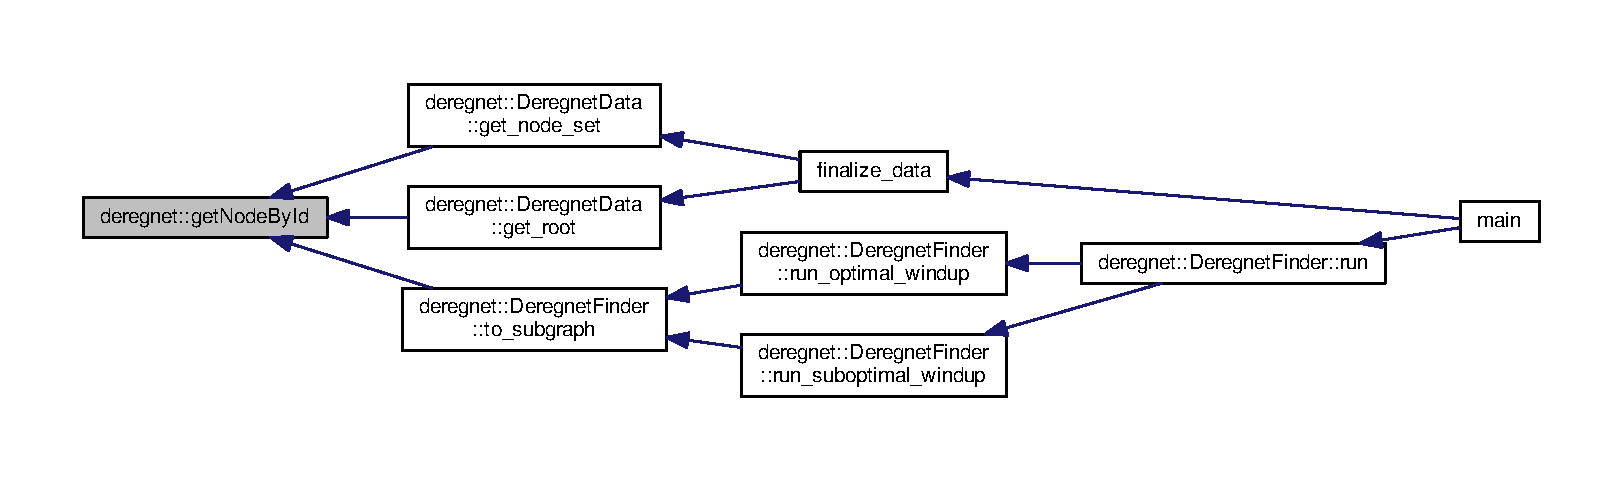
\includegraphics[width=350pt]{namespacederegnet_afefc9088a0ea47e8d8c1225b5de29244_icgraph}
\end{center}
\end{figure}


\index{deregnet@{deregnet}!register\+\_\+node\+\_\+set@{register\+\_\+node\+\_\+set}}
\index{register\+\_\+node\+\_\+set@{register\+\_\+node\+\_\+set}!deregnet@{deregnet}}
\subsubsection[{\texorpdfstring{register\+\_\+node\+\_\+set(std\+::set$<$ std\+::string $>$ $\ast$$\ast$node\+\_\+set, std\+::string comma\+\_\+separated\+\_\+list\+\_\+of\+\_\+nodes)}{register_node_set(std::set< std::string > **node_set, std::string comma_separated_list_of_nodes)}}]{\setlength{\rightskip}{0pt plus 5cm}void deregnet\+::register\+\_\+node\+\_\+set (
\begin{DoxyParamCaption}
\item[{std\+::set$<$ std\+::string $>$ $\ast$$\ast$}]{node\+\_\+set, }
\item[{std\+::string}]{comma\+\_\+separated\+\_\+list\+\_\+of\+\_\+nodes}
\end{DoxyParamCaption}
)}\hypertarget{namespacederegnet_a3ca4926831aa9ca021d1b9230429e8bd}{}\label{namespacederegnet_a3ca4926831aa9ca021d1b9230429e8bd}
\index{deregnet@{deregnet}!register\+\_\+node\+\_\+set@{register\+\_\+node\+\_\+set}}
\index{register\+\_\+node\+\_\+set@{register\+\_\+node\+\_\+set}!deregnet@{deregnet}}
\subsubsection[{\texorpdfstring{register\+\_\+node\+\_\+set(set$<$ string $>$ $\ast$$\ast$node\+\_\+set, string comma\+\_\+separated\+\_\+list\+\_\+of\+\_\+nodes)}{register_node_set(set< string > **node_set, string comma_separated_list_of_nodes)}}]{\setlength{\rightskip}{0pt plus 5cm}void deregnet\+::register\+\_\+node\+\_\+set (
\begin{DoxyParamCaption}
\item[{set$<$ string $>$ $\ast$$\ast$}]{node\+\_\+set, }
\item[{string}]{comma\+\_\+separated\+\_\+list\+\_\+of\+\_\+nodes}
\end{DoxyParamCaption}
)}\hypertarget{namespacederegnet_a639799db7e485ee8cc15b5933be7b4ba}{}\label{namespacederegnet_a639799db7e485ee8cc15b5933be7b4ba}


Definition at line 64 of file utils.\+cpp.



References split\+\_\+string().



Referenced by parse\+\_\+options(), and set\+\_\+union().


\begin{DoxyCode}
65                                                              \{
66     \textcolor{keywordflow}{if} (!(*node\_set))
67         *node\_set = \textcolor{keyword}{new} set<string>( \hyperlink{namespacederegnet_aa12afb18c8703a823fee68c5b9a04bca}{split\_string}(comma\_separated\_list\_of\_nodes, \textcolor{stringliteral}{","}) );
68     \textcolor{keywordflow}{else}
69         set\_union<string>(node\_set, \hyperlink{namespacederegnet_aa12afb18c8703a823fee68c5b9a04bca}{split\_string}(comma\_separated\_list\_of\_nodes, \textcolor{stringliteral}{","}) );
70 \}
\end{DoxyCode}


Here is the call graph for this function\+:\nopagebreak
\begin{figure}[H]
\begin{center}
\leavevmode
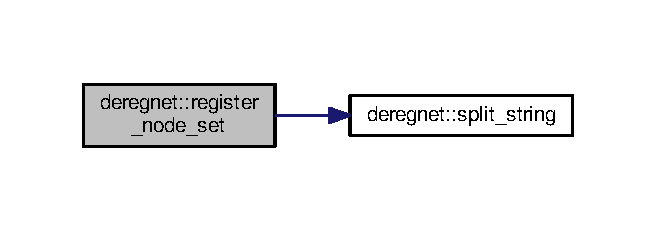
\includegraphics[width=315pt]{namespacederegnet_a639799db7e485ee8cc15b5933be7b4ba_cgraph}
\end{center}
\end{figure}




Here is the caller graph for this function\+:\nopagebreak
\begin{figure}[H]
\begin{center}
\leavevmode
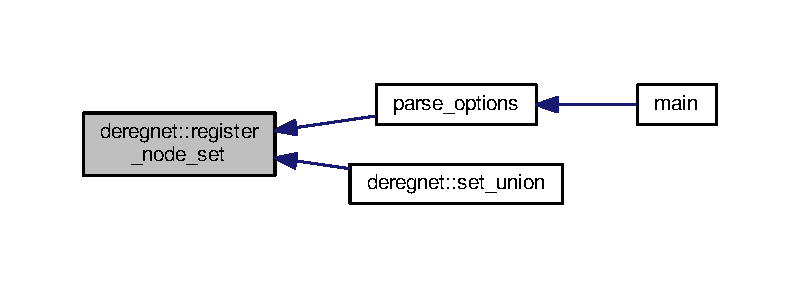
\includegraphics[width=350pt]{namespacederegnet_a639799db7e485ee8cc15b5933be7b4ba_icgraph}
\end{center}
\end{figure}


\index{deregnet@{deregnet}!register\+\_\+node\+\_\+set\+\_\+file@{register\+\_\+node\+\_\+set\+\_\+file}}
\index{register\+\_\+node\+\_\+set\+\_\+file@{register\+\_\+node\+\_\+set\+\_\+file}!deregnet@{deregnet}}
\subsubsection[{\texorpdfstring{register\+\_\+node\+\_\+set\+\_\+file(std\+::set$<$ std\+::string $>$ $\ast$$\ast$node\+\_\+set, std\+::string path2file)}{register_node_set_file(std::set< std::string > **node_set, std::string path2file)}}]{\setlength{\rightskip}{0pt plus 5cm}void deregnet\+::register\+\_\+node\+\_\+set\+\_\+file (
\begin{DoxyParamCaption}
\item[{std\+::set$<$ std\+::string $>$ $\ast$$\ast$}]{node\+\_\+set, }
\item[{std\+::string}]{path2file}
\end{DoxyParamCaption}
)}\hypertarget{namespacederegnet_afbda9b78d4072e2058fdd242c4783cf1}{}\label{namespacederegnet_afbda9b78d4072e2058fdd242c4783cf1}
\index{deregnet@{deregnet}!register\+\_\+node\+\_\+set\+\_\+file@{register\+\_\+node\+\_\+set\+\_\+file}}
\index{register\+\_\+node\+\_\+set\+\_\+file@{register\+\_\+node\+\_\+set\+\_\+file}!deregnet@{deregnet}}
\subsubsection[{\texorpdfstring{register\+\_\+node\+\_\+set\+\_\+file(set$<$ string $>$ $\ast$$\ast$node\+\_\+set, string path2file)}{register_node_set_file(set< string > **node_set, string path2file)}}]{\setlength{\rightskip}{0pt plus 5cm}void deregnet\+::register\+\_\+node\+\_\+set\+\_\+file (
\begin{DoxyParamCaption}
\item[{set$<$ string $>$ $\ast$$\ast$}]{node\+\_\+set, }
\item[{string}]{path2file}
\end{DoxyParamCaption}
)}\hypertarget{namespacederegnet_a11d599a7ac217876cf35b3f6899532c0}{}\label{namespacederegnet_a11d599a7ac217876cf35b3f6899532c0}


Definition at line 74 of file utils.\+cpp.



Referenced by parse\+\_\+options(), and set\+\_\+union().


\begin{DoxyCode}
75                                               \{
76     set<string> nodes\_in\_file;
77     \textcolor{keywordflow}{try} \{
78         ifstream file;
79         file.open( path2file );
80         \textcolor{keywordtype}{string} nodeid;
81         \textcolor{keywordflow}{while} ( !file.eof() ) \{
82             file >> nodeid;
83             nodes\_in\_file.insert(nodeid);
84         \}
85         file.close();
86     \}
87     \textcolor{keywordflow}{catch} ( ... ) \{
88         cerr << \textcolor{stringliteral}{"Could not read file "} << path2file << endl;
89     \}
90     \textcolor{keywordflow}{if} (!(*node\_set))
91         *node\_set = \textcolor{keyword}{new} set<string>(nodes\_in\_file);
92     \textcolor{keywordflow}{else}
93         set\_union<string>(node\_set, nodes\_in\_file);
94 \}
\end{DoxyCode}


Here is the caller graph for this function\+:\nopagebreak
\begin{figure}[H]
\begin{center}
\leavevmode
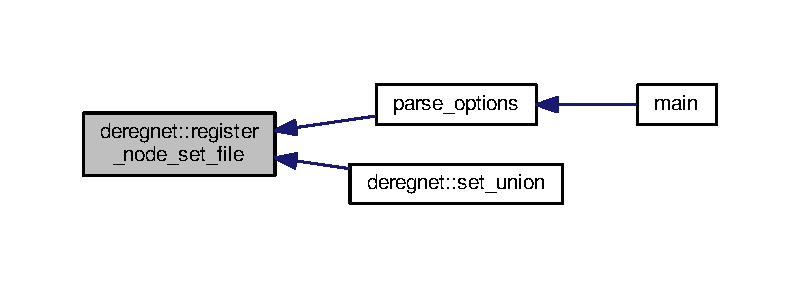
\includegraphics[width=350pt]{namespacederegnet_a11d599a7ac217876cf35b3f6899532c0_icgraph}
\end{center}
\end{figure}


\index{deregnet@{deregnet}!set\+\_\+union@{set\+\_\+union}}
\index{set\+\_\+union@{set\+\_\+union}!deregnet@{deregnet}}
\subsubsection[{\texorpdfstring{set\+\_\+union(std\+::set$<$ T $>$ $\ast$$\ast$\+A, std\+::set$<$ T $>$ B)}{set_union(std::set< T > **A, std::set< T > B)}}]{\setlength{\rightskip}{0pt plus 5cm}template$<$typename T $>$ void deregnet\+::set\+\_\+union (
\begin{DoxyParamCaption}
\item[{std\+::set$<$ T $>$ $\ast$$\ast$}]{A, }
\item[{std\+::set$<$ T $>$}]{B}
\end{DoxyParamCaption}
)}\hypertarget{namespacederegnet_a4358b76b371b698be243476cdabc15ab}{}\label{namespacederegnet_a4358b76b371b698be243476cdabc15ab}


Definition at line 54 of file utils.\+h.



References register\+\_\+node\+\_\+set(), and register\+\_\+node\+\_\+set\+\_\+file().


\begin{DoxyCode}
54                                            \{
55     \textcolor{keywordflow}{for} (\textcolor{keyword}{auto} elmt : B) (*A)->insert(elmt);
56 \}
\end{DoxyCode}


Here is the call graph for this function\+:\nopagebreak
\begin{figure}[H]
\begin{center}
\leavevmode
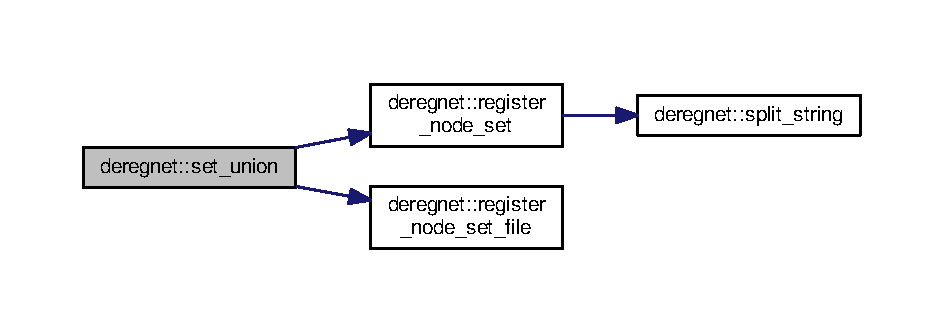
\includegraphics[width=350pt]{namespacederegnet_a4358b76b371b698be243476cdabc15ab_cgraph}
\end{center}
\end{figure}


\index{deregnet@{deregnet}!split\+\_\+string@{split\+\_\+string}}
\index{split\+\_\+string@{split\+\_\+string}!deregnet@{deregnet}}
\subsubsection[{\texorpdfstring{split\+\_\+string(const std\+::string \&str, const std\+::string \&sep)}{split_string(const std::string &str, const std::string &sep)}}]{\setlength{\rightskip}{0pt plus 5cm}std\+::set$<$std\+::string$>$ deregnet\+::split\+\_\+string (
\begin{DoxyParamCaption}
\item[{const std\+::string \&}]{str, }
\item[{const std\+::string \&}]{sep}
\end{DoxyParamCaption}
)}\hypertarget{namespacederegnet_ae4879ebf699f46d51e52b95f1e6f79da}{}\label{namespacederegnet_ae4879ebf699f46d51e52b95f1e6f79da}
\index{deregnet@{deregnet}!split\+\_\+string@{split\+\_\+string}}
\index{split\+\_\+string@{split\+\_\+string}!deregnet@{deregnet}}
\subsubsection[{\texorpdfstring{split\+\_\+string(const string \&str, const string \&sep)}{split_string(const string &str, const string &sep)}}]{\setlength{\rightskip}{0pt plus 5cm}set$<$string$>$ deregnet\+::split\+\_\+string (
\begin{DoxyParamCaption}
\item[{const string \&}]{str, }
\item[{const string \&}]{sep}
\end{DoxyParamCaption}
)}\hypertarget{namespacederegnet_aa12afb18c8703a823fee68c5b9a04bca}{}\label{namespacederegnet_aa12afb18c8703a823fee68c5b9a04bca}


Definition at line 49 of file utils.\+cpp.



Referenced by register\+\_\+node\+\_\+set().


\begin{DoxyCode}
50                                             \{
51     set<string> split;
52     string::size\_type start \{ 0 \};
53     string::size\_type last\_sep \{ 0 \};
54     \textcolor{keywordflow}{while} (last\_sep != string::npos) \{
55         last\_sep = str.find\_first\_of(sep, start);
56         split.insert( str.substr(start, last\_sep - start) );
57         start = last\_sep + 1;
58     \}
59     \textcolor{keywordflow}{return} split;
60 \}
\end{DoxyCode}


Here is the caller graph for this function\+:\nopagebreak
\begin{figure}[H]
\begin{center}
\leavevmode
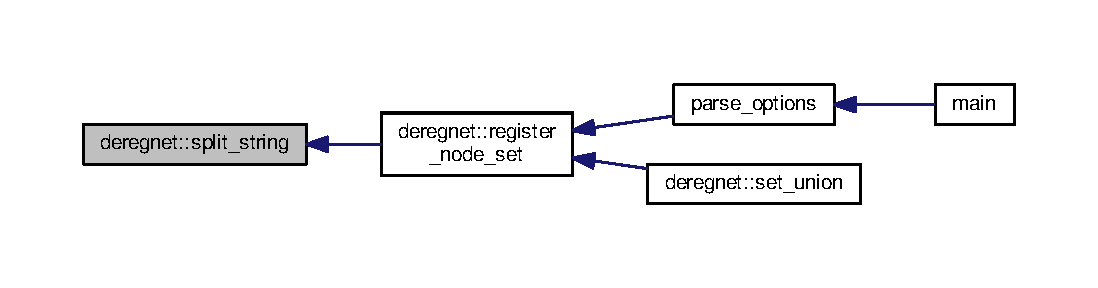
\includegraphics[width=350pt]{namespacederegnet_aa12afb18c8703a823fee68c5b9a04bca_icgraph}
\end{center}
\end{figure}


\index{deregnet@{deregnet}!write2sif@{write2sif}}
\index{write2sif@{write2sif}!deregnet@{deregnet}}
\subsubsection[{\texorpdfstring{write2sif(\+Graph $\ast$graph, std\+::set$<$ Node $>$ \&node\+\_\+set, Node\+Map$<$ std\+::string $>$ $\ast$nodeid, std\+::string path2file)}{write2sif(Graph *graph, std::set< Node > &node_set, NodeMap< std::string > *nodeid, std::string path2file)}}]{\setlength{\rightskip}{0pt plus 5cm}void deregnet\+::write2sif (
\begin{DoxyParamCaption}
\item[{{\bf Graph} $\ast$}]{graph, }
\item[{std\+::set$<$ {\bf Node} $>$ \&}]{node\+\_\+set, }
\item[{{\bf Node\+Map}$<$ std\+::string $>$ $\ast$}]{nodeid, }
\item[{std\+::string}]{path2file}
\end{DoxyParamCaption}
)}\hypertarget{namespacederegnet_a57ac2e918179ec5c93f20248daf39b04}{}\label{namespacederegnet_a57ac2e918179ec5c93f20248daf39b04}


Definition at line 135 of file utils.\+cpp.



References I\+N\+V\+A\+L\+ID.


\begin{DoxyCode}
135                                                                                                       \{
136     ofstream sif\_file;
137     sif\_file.open(path2file);
138     \textcolor{keywordflow}{for} (\textcolor{keyword}{auto} v : node\_set)
139         \textcolor{keywordflow}{for} (\hyperlink{namespacederegnet_a253cef939ea250e4cc0c967cd0117853}{OutArcIt} a(*graph, v); a != \hyperlink{usinglemon_8h_adf770fe2eec438e3758ffe905dbae208}{INVALID}; ++a)
140             \textcolor{keywordflow}{if} (node\_set.find(graph->target(a)) != node\_set.end())
141                 sif\_file << (*nodeid)[v] << \textcolor{stringliteral}{"\(\backslash\)tpp\(\backslash\)t"} << (*nodeid)[graph->target(a)] << \textcolor{stringliteral}{"\(\backslash\)n"};
142     sif\_file.close();
143 \}
\end{DoxyCode}

\chapter{Class Documentation}
\hypertarget{classderegnet_1_1AvgdrgntData}{}\section{deregnet\+:\+:Avgdrgnt\+Data Class Reference}
\label{classderegnet_1_1AvgdrgntData}\index{deregnet\+::\+Avgdrgnt\+Data@{deregnet\+::\+Avgdrgnt\+Data}}


Represents all data and parameters to run the average version of the De\+Reg\+Net.  




{\ttfamily \#include $<$Avgdrgnt\+Data.\+hpp$>$}



Inheritance diagram for deregnet\+:\+:Avgdrgnt\+Data\+:\nopagebreak
\begin{figure}[H]
\begin{center}
\leavevmode
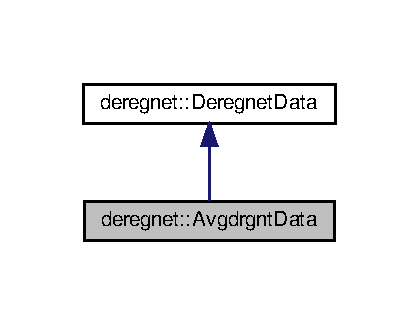
\includegraphics[width=201pt]{classderegnet_1_1AvgdrgntData__inherit__graph}
\end{center}
\end{figure}


Collaboration diagram for deregnet\+:\+:Avgdrgnt\+Data\+:\nopagebreak
\begin{figure}[H]
\begin{center}
\leavevmode
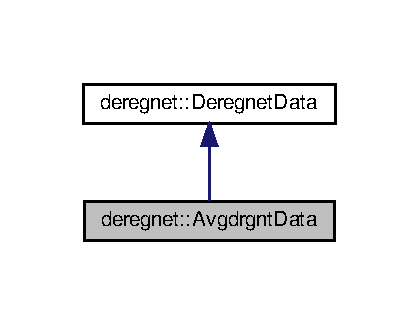
\includegraphics[width=201pt]{classderegnet_1_1AvgdrgntData__coll__graph}
\end{center}
\end{figure}
\subsection*{Public Attributes}
\begin{DoxyCompactItemize}
\item 
int \hyperlink{classderegnet_1_1AvgdrgntData_a733e0cd627433fca043a7f9b70af18c3}{min\+\_\+size} \{ 20 \}
\begin{DoxyCompactList}\small\item\em Minimal size of the resulting subgraphs. \end{DoxyCompactList}\item 
int \hyperlink{classderegnet_1_1AvgdrgntData_a9e844158e12d5e1c4d519c492cffeb17}{max\+\_\+size} \{ 50 \}
\begin{DoxyCompactList}\small\item\em Maximal size of the resulting subgraphs. \end{DoxyCompactList}\item 
int $\ast$ \hyperlink{classderegnet_1_1AvgdrgntData_a38c3bdd86fa3d6ef16ca5db821ca12d2}{min\+\_\+num\+\_\+terminals} \{ nullptr \}
\begin{DoxyCompactList}\small\item\em Minimal number of terminal nodes in subgraphs. \end{DoxyCompactList}\item 
int $\ast$ \hyperlink{classderegnet_1_1AvgdrgntData_a908acb714a65fd9ec4c278fa08150d96}{min\+\_\+num\+\_\+receptors} \{ nullptr \}
\begin{DoxyCompactList}\small\item\em Minimal number of receptor nodes in subgraphs. \end{DoxyCompactList}\item 
\hyperlink{namespacederegnet_ad59156f873b7ab02d384164b900cd874}{Algorithm} \hyperlink{classderegnet_1_1AvgdrgntData_aa75d6acc2d63aa589651c705eaf89280}{algorithm} \{ Algorithm\+::\+D\+TA \}
\begin{DoxyCompactList}\small\item\em Which solution algorithm to employ. \end{DoxyCompactList}\end{DoxyCompactItemize}
\subsection*{Additional Inherited Members}


\subsection{Detailed Description}
Represents all data and parameters to run the average version of the De\+Reg\+Net. 

Definition at line 51 of file Avgdrgnt\+Data.\+hpp.



\subsection{Member Data Documentation}
\mbox{\Hypertarget{classderegnet_1_1AvgdrgntData_aa75d6acc2d63aa589651c705eaf89280}\label{classderegnet_1_1AvgdrgntData_aa75d6acc2d63aa589651c705eaf89280}} 
\index{deregnet\+::\+Avgdrgnt\+Data@{deregnet\+::\+Avgdrgnt\+Data}!algorithm@{algorithm}}
\index{algorithm@{algorithm}!deregnet\+::\+Avgdrgnt\+Data@{deregnet\+::\+Avgdrgnt\+Data}}
\subsubsection{\texorpdfstring{algorithm}{algorithm}}
{\footnotesize\ttfamily \hyperlink{namespacederegnet_ad59156f873b7ab02d384164b900cd874}{Algorithm} deregnet\+::\+Avgdrgnt\+Data\+::algorithm \{ Algorithm\+::\+D\+TA \}}



Which solution algorithm to employ. 



Definition at line 61 of file Avgdrgnt\+Data.\+hpp.



Referenced by finalize\+\_\+data(), and parse\+\_\+options().

\mbox{\Hypertarget{classderegnet_1_1AvgdrgntData_a9e844158e12d5e1c4d519c492cffeb17}\label{classderegnet_1_1AvgdrgntData_a9e844158e12d5e1c4d519c492cffeb17}} 
\index{deregnet\+::\+Avgdrgnt\+Data@{deregnet\+::\+Avgdrgnt\+Data}!max\+\_\+size@{max\+\_\+size}}
\index{max\+\_\+size@{max\+\_\+size}!deregnet\+::\+Avgdrgnt\+Data@{deregnet\+::\+Avgdrgnt\+Data}}
\subsubsection{\texorpdfstring{max\+\_\+size}{max\_size}}
{\footnotesize\ttfamily int deregnet\+::\+Avgdrgnt\+Data\+::max\+\_\+size \{ 50 \}}



Maximal size of the resulting subgraphs. 



Definition at line 56 of file Avgdrgnt\+Data.\+hpp.



Referenced by finalize\+\_\+data(), deregnet\+::\+Deregnet\+Finder$<$ Model\+Type, Data $>$\+::find\+\_\+start\+\_\+solution(), deregnet\+::\+Deregnet\+Finder$<$ Model\+Type, Data $>$\+::find\+\_\+suboptimal\+\_\+start\+\_\+solution(), and parse\+\_\+options().

\mbox{\Hypertarget{classderegnet_1_1AvgdrgntData_a908acb714a65fd9ec4c278fa08150d96}\label{classderegnet_1_1AvgdrgntData_a908acb714a65fd9ec4c278fa08150d96}} 
\index{deregnet\+::\+Avgdrgnt\+Data@{deregnet\+::\+Avgdrgnt\+Data}!min\+\_\+num\+\_\+receptors@{min\+\_\+num\+\_\+receptors}}
\index{min\+\_\+num\+\_\+receptors@{min\+\_\+num\+\_\+receptors}!deregnet\+::\+Avgdrgnt\+Data@{deregnet\+::\+Avgdrgnt\+Data}}
\subsubsection{\texorpdfstring{min\+\_\+num\+\_\+receptors}{min\_num\_receptors}}
{\footnotesize\ttfamily int$\ast$ deregnet\+::\+Avgdrgnt\+Data\+::min\+\_\+num\+\_\+receptors \{ nullptr \}}



Minimal number of receptor nodes in subgraphs. 



Definition at line 59 of file Avgdrgnt\+Data.\+hpp.

\mbox{\Hypertarget{classderegnet_1_1AvgdrgntData_a38c3bdd86fa3d6ef16ca5db821ca12d2}\label{classderegnet_1_1AvgdrgntData_a38c3bdd86fa3d6ef16ca5db821ca12d2}} 
\index{deregnet\+::\+Avgdrgnt\+Data@{deregnet\+::\+Avgdrgnt\+Data}!min\+\_\+num\+\_\+terminals@{min\+\_\+num\+\_\+terminals}}
\index{min\+\_\+num\+\_\+terminals@{min\+\_\+num\+\_\+terminals}!deregnet\+::\+Avgdrgnt\+Data@{deregnet\+::\+Avgdrgnt\+Data}}
\subsubsection{\texorpdfstring{min\+\_\+num\+\_\+terminals}{min\_num\_terminals}}
{\footnotesize\ttfamily int$\ast$ deregnet\+::\+Avgdrgnt\+Data\+::min\+\_\+num\+\_\+terminals \{ nullptr \}}



Minimal number of terminal nodes in subgraphs. 



Definition at line 58 of file Avgdrgnt\+Data.\+hpp.



Referenced by parse\+\_\+options().

\mbox{\Hypertarget{classderegnet_1_1AvgdrgntData_a733e0cd627433fca043a7f9b70af18c3}\label{classderegnet_1_1AvgdrgntData_a733e0cd627433fca043a7f9b70af18c3}} 
\index{deregnet\+::\+Avgdrgnt\+Data@{deregnet\+::\+Avgdrgnt\+Data}!min\+\_\+size@{min\+\_\+size}}
\index{min\+\_\+size@{min\+\_\+size}!deregnet\+::\+Avgdrgnt\+Data@{deregnet\+::\+Avgdrgnt\+Data}}
\subsubsection{\texorpdfstring{min\+\_\+size}{min\_size}}
{\footnotesize\ttfamily int deregnet\+::\+Avgdrgnt\+Data\+::min\+\_\+size \{ 20 \}}



Minimal size of the resulting subgraphs. 



Definition at line 55 of file Avgdrgnt\+Data.\+hpp.



Referenced by deregnet\+::\+Deregnet\+Finder$<$ Model\+Type, Data $>$\+::find\+\_\+start\+\_\+solution(), deregnet\+::\+Deregnet\+Finder$<$ Model\+Type, Data $>$\+::find\+\_\+suboptimal\+\_\+start\+\_\+solution(), and parse\+\_\+options().



The documentation for this class was generated from the following file\+:\begin{DoxyCompactItemize}
\item 
/datadisk/bbubu/home/self/bbubu/projects/deregnet/src/\hyperlink{AvgdrgntData_8hpp}{Avgdrgnt\+Data.\+hpp}\end{DoxyCompactItemize}

\hypertarget{classderegnet_1_1AvgStartHeuristic}{}\section{deregnet\+:\+:Avg\+Start\+Heuristic Class Reference}
\label{classderegnet_1_1AvgStartHeuristic}\index{deregnet\+::\+Avg\+Start\+Heuristic@{deregnet\+::\+Avg\+Start\+Heuristic}}


Implementation of the heuristic solution algorithm for average De\+Reg\+Net algorithm.  




{\ttfamily \#include $<$Avg\+Start\+Heuristic.\+hpp$>$}



Inheritance diagram for deregnet\+:\+:Avg\+Start\+Heuristic\+:\nopagebreak
\begin{figure}[H]
\begin{center}
\leavevmode
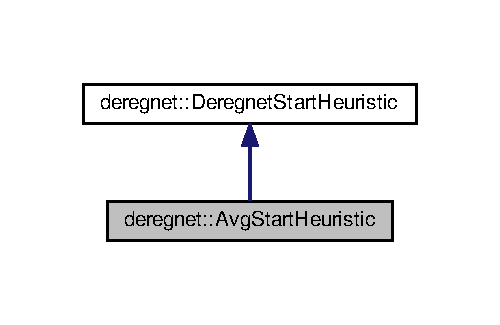
\includegraphics[width=240pt]{classderegnet_1_1AvgStartHeuristic__inherit__graph}
\end{center}
\end{figure}


Collaboration diagram for deregnet\+:\+:Avg\+Start\+Heuristic\+:\nopagebreak
\begin{figure}[H]
\begin{center}
\leavevmode
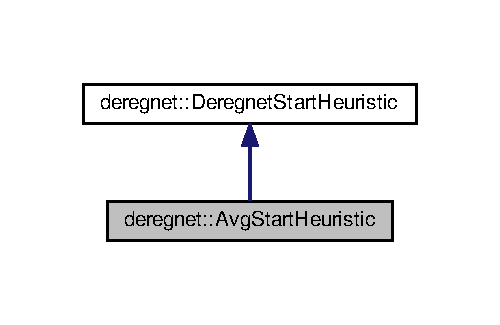
\includegraphics[width=240pt]{classderegnet_1_1AvgStartHeuristic__coll__graph}
\end{center}
\end{figure}
\subsection*{Public Member Functions}
\begin{DoxyCompactItemize}
\item 
\hyperlink{classderegnet_1_1AvgStartHeuristic_afcbb54f71a6277598a40d6c06ebddbf0}{Avg\+Start\+Heuristic} (\hyperlink{namespacederegnet_a55b76c55bbabc682cbc61f8b9948799e}{Graph} $\ast$xgraph, \hyperlink{namespacederegnet_ae102b707ae1d6f83c639ece5e0dd5658}{Node\+Map}$<$ double $>$ $\ast$xscore, \hyperlink{namespacederegnet_a744bad34f2de9856d36715a445f027f3}{Node} $\ast$\hyperlink{classderegnet_1_1DeregnetStartHeuristic_a4605d41352e3adf1f9f9f32466a4e61e}{root}, std\+::set$<$ \hyperlink{namespacederegnet_a744bad34f2de9856d36715a445f027f3}{Node} $>$ $\ast$\hyperlink{classderegnet_1_1DeregnetStartHeuristic_aa22c6581cd404bf7ac325850b28dc951}{exclude}, std\+::set$<$ \hyperlink{namespacederegnet_a744bad34f2de9856d36715a445f027f3}{Node} $>$ $\ast$\hyperlink{classderegnet_1_1DeregnetStartHeuristic_ab80c046ff2b7c64086fceb84987b3e50}{receptors}, std\+::function$<$ bool(double, double)$>$ xcmp, int xmin\+\_\+size, int xmax\+\_\+size)
\end{DoxyCompactItemize}
\subsection*{Private Member Functions}
\begin{DoxyCompactItemize}
\item 
virtual \hyperlink{namespacederegnet_a744bad34f2de9856d36715a445f027f3}{Node} $\ast$ \hyperlink{classderegnet_1_1AvgStartHeuristic_ac13190b98b5611ad231fe3d9447431fb}{get\+\_\+best\+\_\+root} () override
\begin{DoxyCompactList}\small\item\em Find best node to add to solution in every iteration. \end{DoxyCompactList}\item 
virtual bool \hyperlink{classderegnet_1_1AvgStartHeuristic_a6fcfd578c66c01240d3484513a34bef6}{search\+\_\+further} () override
\begin{DoxyCompactList}\small\item\em Decide whether to continue searching further (for other solution than the one already found) \end{DoxyCompactList}\item 
virtual bool \hyperlink{classderegnet_1_1AvgStartHeuristic_a3e18528bc735d47edcd719a72baf4e46}{feasible\+\_\+node} (\hyperlink{namespacederegnet_a744bad34f2de9856d36715a445f027f3}{Node} $\ast$node) override
\begin{DoxyCompactList}\small\item\em Decide whether adding a given node to the solution is feasible wrt the given constraints. \end{DoxyCompactList}\item 
double \hyperlink{classderegnet_1_1AvgStartHeuristic_ab3cbc873952af7525654194a7d5e59e0}{update\+\_\+avg} (\hyperlink{namespacederegnet_a744bad34f2de9856d36715a445f027f3}{Node} $\ast$node)
\end{DoxyCompactItemize}
\subsection*{Private Attributes}
\begin{DoxyCompactItemize}
\item 
int \hyperlink{classderegnet_1_1AvgStartHeuristic_a3abc4d801d4eb1fdb8ecfed7077045b3}{min\+\_\+size}
\item 
int \hyperlink{classderegnet_1_1AvgStartHeuristic_a4794e58ea33d94f9029defa3a31cc573}{max\+\_\+size}
\item 
double \hyperlink{classderegnet_1_1AvgStartHeuristic_a2c4b3fa6aa7946276404e650ea42fd14}{current\+\_\+avg} \{ 0.\+0 \}
\end{DoxyCompactItemize}
\subsection*{Additional Inherited Members}


\subsection{Detailed Description}
Implementation of the heuristic solution algorithm for average De\+Reg\+Net algorithm. 

Definition at line 49 of file Avg\+Start\+Heuristic.\+hpp.



\subsection{Constructor \& Destructor Documentation}
\mbox{\Hypertarget{classderegnet_1_1AvgStartHeuristic_afcbb54f71a6277598a40d6c06ebddbf0}\label{classderegnet_1_1AvgStartHeuristic_afcbb54f71a6277598a40d6c06ebddbf0}} 
\index{deregnet\+::\+Avg\+Start\+Heuristic@{deregnet\+::\+Avg\+Start\+Heuristic}!Avg\+Start\+Heuristic@{Avg\+Start\+Heuristic}}
\index{Avg\+Start\+Heuristic@{Avg\+Start\+Heuristic}!deregnet\+::\+Avg\+Start\+Heuristic@{deregnet\+::\+Avg\+Start\+Heuristic}}
\subsubsection{\texorpdfstring{Avg\+Start\+Heuristic()}{AvgStartHeuristic()}}
{\footnotesize\ttfamily deregnet\+::\+Avg\+Start\+Heuristic\+::\+Avg\+Start\+Heuristic (\begin{DoxyParamCaption}\item[{\hyperlink{namespacederegnet_a55b76c55bbabc682cbc61f8b9948799e}{Graph} $\ast$}]{xgraph,  }\item[{\hyperlink{namespacederegnet_ae102b707ae1d6f83c639ece5e0dd5658}{Node\+Map}$<$ double $>$ $\ast$}]{xscore,  }\item[{\hyperlink{namespacederegnet_a744bad34f2de9856d36715a445f027f3}{Node} $\ast$}]{root,  }\item[{std\+::set$<$ \hyperlink{namespacederegnet_a744bad34f2de9856d36715a445f027f3}{Node} $>$ $\ast$}]{exclude,  }\item[{std\+::set$<$ \hyperlink{namespacederegnet_a744bad34f2de9856d36715a445f027f3}{Node} $>$ $\ast$}]{receptors,  }\item[{std\+::function$<$ bool(double, double)$>$}]{xcmp,  }\item[{int}]{xmin\+\_\+size,  }\item[{int}]{xmax\+\_\+size }\end{DoxyParamCaption})}


\begin{DoxyParams}{Parameters}
{\em xgraph} & \\
\hline
{\em xscore} & \\
\hline
{\em root} & \\
\hline
{\em exclude} & \\
\hline
{\em receptors} & \\
\hline
{\em xcmp} & \\
\hline
{\em xmin\+\_\+size} & \\
\hline
{\em xmax\+\_\+size} & \\
\hline
\end{DoxyParams}


Definition at line 42 of file Avg\+Start\+Heuristic.\+cpp.



References max\+\_\+size.


\begin{DoxyCode}
50  : \hyperlink{classderegnet_1_1DeregnetStartHeuristic_af7fa694b10f54c669fce9431214ffc98}{DeregnetStartHeuristic}(xgraph, xscore, \hyperlink{classderegnet_1_1DeregnetStartHeuristic_a4605d41352e3adf1f9f9f32466a4e61e}{root}, 
      \hyperlink{classderegnet_1_1DeregnetStartHeuristic_aa22c6581cd404bf7ac325850b28dc951}{exclude}, \hyperlink{classderegnet_1_1DeregnetStartHeuristic_ab80c046ff2b7c64086fceb84987b3e50}{receptors}, xcmp),
51    \hyperlink{classderegnet_1_1AvgStartHeuristic_a3abc4d801d4eb1fdb8ecfed7077045b3}{min\_size} \{ xmin\_size \},
52    \hyperlink{classderegnet_1_1AvgStartHeuristic_a4794e58ea33d94f9029defa3a31cc573}{max\_size} \{ xmax\_size \}
53 \{ \}
\end{DoxyCode}


\subsection{Member Function Documentation}
\mbox{\Hypertarget{classderegnet_1_1AvgStartHeuristic_a3e18528bc735d47edcd719a72baf4e46}\label{classderegnet_1_1AvgStartHeuristic_a3e18528bc735d47edcd719a72baf4e46}} 
\index{deregnet\+::\+Avg\+Start\+Heuristic@{deregnet\+::\+Avg\+Start\+Heuristic}!feasible\+\_\+node@{feasible\+\_\+node}}
\index{feasible\+\_\+node@{feasible\+\_\+node}!deregnet\+::\+Avg\+Start\+Heuristic@{deregnet\+::\+Avg\+Start\+Heuristic}}
\subsubsection{\texorpdfstring{feasible\+\_\+node()}{feasible\_node()}}
{\footnotesize\ttfamily bool deregnet\+::\+Avg\+Start\+Heuristic\+::feasible\+\_\+node (\begin{DoxyParamCaption}\item[{\hyperlink{namespacederegnet_a744bad34f2de9856d36715a445f027f3}{Node} $\ast$}]{node }\end{DoxyParamCaption})\hspace{0.3cm}{\ttfamily [override]}, {\ttfamily [private]}, {\ttfamily [virtual]}}



Decide whether adding a given node to the solution is feasible wrt the given constraints. 


\begin{DoxyParams}{Parameters}
{\em node} & A node in the graph\\
\hline
\end{DoxyParams}
\begin{DoxyReturn}{Returns}
Whether adding the node is feasible 
\end{DoxyReturn}


Implements \hyperlink{classderegnet_1_1DeregnetStartHeuristic_ac296c4f122f7d3ad2fcc2cbb0d1b5379}{deregnet\+::\+Deregnet\+Start\+Heuristic}.



Definition at line 91 of file Avg\+Start\+Heuristic.\+cpp.



References current\+\_\+avg, min\+\_\+size, deregnet\+::\+Deregnet\+Start\+Heuristic\+::start\+\_\+solution, and update\+\_\+avg().


\begin{DoxyCode}
91                                                 \{
92     \textcolor{keywordtype}{double} new\_avg \{ \hyperlink{classderegnet_1_1AvgStartHeuristic_ab3cbc873952af7525654194a7d5e59e0}{update\_avg}(node) \};
93     \textcolor{keywordtype}{int} current\_size \{ \textcolor{keyword}{static\_cast<}\textcolor{keywordtype}{int}\textcolor{keyword}{>}(\hyperlink{classderegnet_1_1DeregnetStartHeuristic_a7450e11ca0a265b055f95e7832b65e2f}{start\_solution}->size()) \};
94     \textcolor{keywordflow}{if} (current\_size >= \hyperlink{classderegnet_1_1AvgStartHeuristic_a3abc4d801d4eb1fdb8ecfed7077045b3}{min\_size} && new\_avg < \hyperlink{classderegnet_1_1AvgStartHeuristic_a2c4b3fa6aa7946276404e650ea42fd14}{current\_avg})
95         \textcolor{keywordflow}{return} \textcolor{keyword}{false};
96     \hyperlink{classderegnet_1_1AvgStartHeuristic_a2c4b3fa6aa7946276404e650ea42fd14}{current\_avg} = new\_avg;
97     \textcolor{keywordflow}{if} (\hyperlink{classderegnet_1_1DeregnetStartHeuristic_aa22c6581cd404bf7ac325850b28dc951}{exclude}) \{
98         \textcolor{keywordflow}{if} (\hyperlink{classderegnet_1_1DeregnetStartHeuristic_a7450e11ca0a265b055f95e7832b65e2f}{start\_solution}->find(*node) == \hyperlink{classderegnet_1_1DeregnetStartHeuristic_a7450e11ca0a265b055f95e7832b65e2f}{start\_solution}->end() &&
99             \hyperlink{classderegnet_1_1DeregnetStartHeuristic_aa22c6581cd404bf7ac325850b28dc951}{exclude}->find(*node) == \hyperlink{classderegnet_1_1DeregnetStartHeuristic_aa22c6581cd404bf7ac325850b28dc951}{exclude}->end()) \{
100             \textcolor{keywordflow}{return} \textcolor{keyword}{true};
101         \}
102     \}
103     \textcolor{keywordflow}{else}
104         \textcolor{keywordflow}{if} (\hyperlink{classderegnet_1_1DeregnetStartHeuristic_a7450e11ca0a265b055f95e7832b65e2f}{start\_solution}->find(*node) == \hyperlink{classderegnet_1_1DeregnetStartHeuristic_a7450e11ca0a265b055f95e7832b65e2f}{start\_solution}->end())
105             \textcolor{keywordflow}{return} \textcolor{keyword}{true};
106     \textcolor{keywordflow}{return} \textcolor{keyword}{false};
107 \}
\end{DoxyCode}
Here is the call graph for this function\+:\nopagebreak
\begin{figure}[H]
\begin{center}
\leavevmode
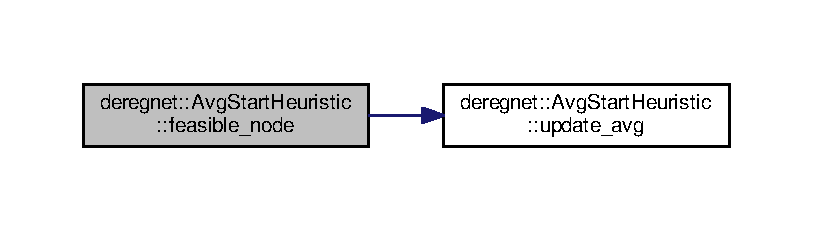
\includegraphics[width=350pt]{classderegnet_1_1AvgStartHeuristic_a3e18528bc735d47edcd719a72baf4e46_cgraph}
\end{center}
\end{figure}
\mbox{\Hypertarget{classderegnet_1_1AvgStartHeuristic_ac13190b98b5611ad231fe3d9447431fb}\label{classderegnet_1_1AvgStartHeuristic_ac13190b98b5611ad231fe3d9447431fb}} 
\index{deregnet\+::\+Avg\+Start\+Heuristic@{deregnet\+::\+Avg\+Start\+Heuristic}!get\+\_\+best\+\_\+root@{get\+\_\+best\+\_\+root}}
\index{get\+\_\+best\+\_\+root@{get\+\_\+best\+\_\+root}!deregnet\+::\+Avg\+Start\+Heuristic@{deregnet\+::\+Avg\+Start\+Heuristic}}
\subsubsection{\texorpdfstring{get\+\_\+best\+\_\+root()}{get\_best\_root()}}
{\footnotesize\ttfamily \hyperlink{namespacederegnet_a744bad34f2de9856d36715a445f027f3}{Node} $\ast$ deregnet\+::\+Avg\+Start\+Heuristic\+::get\+\_\+best\+\_\+root (\begin{DoxyParamCaption}{ }\end{DoxyParamCaption})\hspace{0.3cm}{\ttfamily [override]}, {\ttfamily [private]}, {\ttfamily [virtual]}}



Find best node to add to solution in every iteration. 

\begin{DoxyReturn}{Returns}
The best node to add 
\end{DoxyReturn}


Implements \hyperlink{classderegnet_1_1DeregnetStartHeuristic_a372be86d0fb8ac94bd926a1f4d09e102}{deregnet\+::\+Deregnet\+Start\+Heuristic}.



Definition at line 55 of file Avg\+Start\+Heuristic.\+cpp.



References deregnet\+::\+Deregnet\+Start\+Heuristic\+::graph, I\+N\+V\+A\+L\+ID, and deregnet\+::\+Deregnet\+Start\+Heuristic\+::update\+\_\+best\+\_\+node().


\begin{DoxyCode}
55                                        \{
56     \textcolor{keywordtype}{double} best;
57     \hyperlink{namespacederegnet_a744bad34f2de9856d36715a445f027f3}{Node}* best\_node \{ \textcolor{keyword}{nullptr} \};
58     \textcolor{keywordflow}{if} (\hyperlink{classderegnet_1_1DeregnetStartHeuristic_ab80c046ff2b7c64086fceb84987b3e50}{receptors})
59         \textcolor{keywordflow}{for} (\textcolor{keyword}{auto} v : *\hyperlink{classderegnet_1_1DeregnetStartHeuristic_ab80c046ff2b7c64086fceb84987b3e50}{receptors})
60             \hyperlink{classderegnet_1_1DeregnetStartHeuristic_a50179ff9db4d416b93ff41d1dcee1358}{update\_best\_node}(&best\_node, &v, &best);
61     \textcolor{keywordflow}{else}
62         \textcolor{keywordflow}{for} (\hyperlink{namespacederegnet_ac34314e1b5f456fc6d1bb9d96316de4a}{NodeIt} v(*\hyperlink{classderegnet_1_1DeregnetStartHeuristic_a4da8e53fc7c0fa3dbe0e3ef07296d75e}{graph}); v != \hyperlink{usinglemon_8hpp_adf770fe2eec438e3758ffe905dbae208}{INVALID}; ++v)
63             \hyperlink{classderegnet_1_1DeregnetStartHeuristic_a50179ff9db4d416b93ff41d1dcee1358}{update\_best\_node}(&best\_node, &v, &best);
64     \textcolor{keywordflow}{return} best\_node;
65 \}
\end{DoxyCode}
Here is the call graph for this function\+:\nopagebreak
\begin{figure}[H]
\begin{center}
\leavevmode
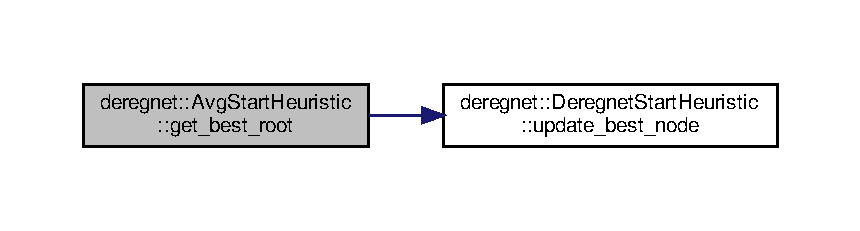
\includegraphics[width=350pt]{classderegnet_1_1AvgStartHeuristic_ac13190b98b5611ad231fe3d9447431fb_cgraph}
\end{center}
\end{figure}
\mbox{\Hypertarget{classderegnet_1_1AvgStartHeuristic_a6fcfd578c66c01240d3484513a34bef6}\label{classderegnet_1_1AvgStartHeuristic_a6fcfd578c66c01240d3484513a34bef6}} 
\index{deregnet\+::\+Avg\+Start\+Heuristic@{deregnet\+::\+Avg\+Start\+Heuristic}!search\+\_\+further@{search\+\_\+further}}
\index{search\+\_\+further@{search\+\_\+further}!deregnet\+::\+Avg\+Start\+Heuristic@{deregnet\+::\+Avg\+Start\+Heuristic}}
\subsubsection{\texorpdfstring{search\+\_\+further()}{search\_further()}}
{\footnotesize\ttfamily bool deregnet\+::\+Avg\+Start\+Heuristic\+::search\+\_\+further (\begin{DoxyParamCaption}{ }\end{DoxyParamCaption})\hspace{0.3cm}{\ttfamily [override]}, {\ttfamily [private]}, {\ttfamily [virtual]}}



Decide whether to continue searching further (for other solution than the one already found) 

\begin{DoxyReturn}{Returns}
Whether to search further 
\end{DoxyReturn}


Implements \hyperlink{classderegnet_1_1DeregnetStartHeuristic_ac3ee2c3022512f9d4ec7a6b49358e60a}{deregnet\+::\+Deregnet\+Start\+Heuristic}.



Definition at line 68 of file Avg\+Start\+Heuristic.\+cpp.



References deregnet\+::\+Deregnet\+Start\+Heuristic\+::found\+\_\+node, max\+\_\+size, min\+\_\+size, deregnet\+::\+Deregnet\+Start\+Heuristic\+::start\+\_\+solution, and deregnet\+::\+Deregnet\+Start\+Heuristic\+::success.


\begin{DoxyCode}
68                                        \{
69     \textcolor{keywordtype}{int} current\_size \{ \textcolor{keyword}{static\_cast<}\textcolor{keywordtype}{int}\textcolor{keyword}{>}(\hyperlink{classderegnet_1_1DeregnetStartHeuristic_a7450e11ca0a265b055f95e7832b65e2f}{start\_solution}->size()) \};
70     \textcolor{keywordflow}{if} (current\_size < \hyperlink{classderegnet_1_1AvgStartHeuristic_a3abc4d801d4eb1fdb8ecfed7077045b3}{min\_size}) \{
71         \textcolor{keywordflow}{if} (\hyperlink{classderegnet_1_1DeregnetStartHeuristic_a1ca705794583fb3b6e563efeceb4445e}{found\_node})
72             \textcolor{keywordflow}{return} \textcolor{keyword}{true};
73         \textcolor{keywordflow}{else}
74             \textcolor{keywordflow}{return} \textcolor{keyword}{false};
75     \}
76     \textcolor{keywordflow}{if} (current\_size >= \hyperlink{classderegnet_1_1AvgStartHeuristic_a3abc4d801d4eb1fdb8ecfed7077045b3}{min\_size} && current\_size < \hyperlink{classderegnet_1_1AvgStartHeuristic_a4794e58ea33d94f9029defa3a31cc573}{max\_size}) \{
77         \textcolor{keywordflow}{if} (\hyperlink{classderegnet_1_1DeregnetStartHeuristic_a1ca705794583fb3b6e563efeceb4445e}{found\_node})
78             \textcolor{keywordflow}{return} \textcolor{keyword}{true};
79         \textcolor{keywordflow}{else} \{
80             \hyperlink{classderegnet_1_1DeregnetStartHeuristic_a72fd16ee027f6aa973f1ff29746addba}{success} = \textcolor{keyword}{true};
81             \textcolor{keywordflow}{return} \textcolor{keyword}{false};
82         \}
83     \}
84     \textcolor{keywordflow}{if} (current\_size == \hyperlink{classderegnet_1_1AvgStartHeuristic_a4794e58ea33d94f9029defa3a31cc573}{max\_size}) \{
85         \hyperlink{classderegnet_1_1DeregnetStartHeuristic_a72fd16ee027f6aa973f1ff29746addba}{success} = \textcolor{keyword}{true};
86         \textcolor{keywordflow}{return} \textcolor{keyword}{false};
87     \}
88     \textcolor{keywordflow}{return} \textcolor{keyword}{false};   \textcolor{comment}{// to get rid of compiler warning ... ;)}
89 \}
\end{DoxyCode}
\mbox{\Hypertarget{classderegnet_1_1AvgStartHeuristic_ab3cbc873952af7525654194a7d5e59e0}\label{classderegnet_1_1AvgStartHeuristic_ab3cbc873952af7525654194a7d5e59e0}} 
\index{deregnet\+::\+Avg\+Start\+Heuristic@{deregnet\+::\+Avg\+Start\+Heuristic}!update\+\_\+avg@{update\+\_\+avg}}
\index{update\+\_\+avg@{update\+\_\+avg}!deregnet\+::\+Avg\+Start\+Heuristic@{deregnet\+::\+Avg\+Start\+Heuristic}}
\subsubsection{\texorpdfstring{update\+\_\+avg()}{update\_avg()}}
{\footnotesize\ttfamily double deregnet\+::\+Avg\+Start\+Heuristic\+::update\+\_\+avg (\begin{DoxyParamCaption}\item[{\hyperlink{namespacederegnet_a744bad34f2de9856d36715a445f027f3}{Node} $\ast$}]{node }\end{DoxyParamCaption})\hspace{0.3cm}{\ttfamily [private]}}



Definition at line 109 of file Avg\+Start\+Heuristic.\+cpp.



References current\+\_\+avg, deregnet\+::\+Deregnet\+Start\+Heuristic\+::score, and deregnet\+::\+Deregnet\+Start\+Heuristic\+::start\+\_\+solution.



Referenced by feasible\+\_\+node().


\begin{DoxyCode}
109                                                \{
110     \textcolor{keywordtype}{int} current\_size \{ \textcolor{keyword}{static\_cast<}\textcolor{keywordtype}{int}\textcolor{keyword}{>}(\hyperlink{classderegnet_1_1DeregnetStartHeuristic_a7450e11ca0a265b055f95e7832b65e2f}{start\_solution}->size()) \};
111     \textcolor{keywordflow}{return} ((*\hyperlink{classderegnet_1_1DeregnetStartHeuristic_ae03300e79482975e98f95cba19ad32b0}{score})[*node] + current\_size * \hyperlink{classderegnet_1_1AvgStartHeuristic_a2c4b3fa6aa7946276404e650ea42fd14}{current\_avg}) / (current\_size + 1);
112 \}
\end{DoxyCode}
Here is the caller graph for this function\+:\nopagebreak
\begin{figure}[H]
\begin{center}
\leavevmode
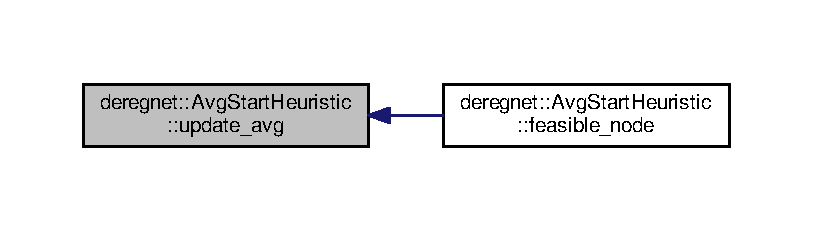
\includegraphics[width=350pt]{classderegnet_1_1AvgStartHeuristic_ab3cbc873952af7525654194a7d5e59e0_icgraph}
\end{center}
\end{figure}


\subsection{Member Data Documentation}
\mbox{\Hypertarget{classderegnet_1_1AvgStartHeuristic_a2c4b3fa6aa7946276404e650ea42fd14}\label{classderegnet_1_1AvgStartHeuristic_a2c4b3fa6aa7946276404e650ea42fd14}} 
\index{deregnet\+::\+Avg\+Start\+Heuristic@{deregnet\+::\+Avg\+Start\+Heuristic}!current\+\_\+avg@{current\+\_\+avg}}
\index{current\+\_\+avg@{current\+\_\+avg}!deregnet\+::\+Avg\+Start\+Heuristic@{deregnet\+::\+Avg\+Start\+Heuristic}}
\subsubsection{\texorpdfstring{current\+\_\+avg}{current\_avg}}
{\footnotesize\ttfamily double deregnet\+::\+Avg\+Start\+Heuristic\+::current\+\_\+avg \{ 0.\+0 \}\hspace{0.3cm}{\ttfamily [private]}}



Definition at line 55 of file Avg\+Start\+Heuristic.\+hpp.



Referenced by feasible\+\_\+node(), and update\+\_\+avg().

\mbox{\Hypertarget{classderegnet_1_1AvgStartHeuristic_a4794e58ea33d94f9029defa3a31cc573}\label{classderegnet_1_1AvgStartHeuristic_a4794e58ea33d94f9029defa3a31cc573}} 
\index{deregnet\+::\+Avg\+Start\+Heuristic@{deregnet\+::\+Avg\+Start\+Heuristic}!max\+\_\+size@{max\+\_\+size}}
\index{max\+\_\+size@{max\+\_\+size}!deregnet\+::\+Avg\+Start\+Heuristic@{deregnet\+::\+Avg\+Start\+Heuristic}}
\subsubsection{\texorpdfstring{max\+\_\+size}{max\_size}}
{\footnotesize\ttfamily int deregnet\+::\+Avg\+Start\+Heuristic\+::max\+\_\+size\hspace{0.3cm}{\ttfamily [private]}}



Definition at line 54 of file Avg\+Start\+Heuristic.\+hpp.



Referenced by Avg\+Start\+Heuristic(), and search\+\_\+further().

\mbox{\Hypertarget{classderegnet_1_1AvgStartHeuristic_a3abc4d801d4eb1fdb8ecfed7077045b3}\label{classderegnet_1_1AvgStartHeuristic_a3abc4d801d4eb1fdb8ecfed7077045b3}} 
\index{deregnet\+::\+Avg\+Start\+Heuristic@{deregnet\+::\+Avg\+Start\+Heuristic}!min\+\_\+size@{min\+\_\+size}}
\index{min\+\_\+size@{min\+\_\+size}!deregnet\+::\+Avg\+Start\+Heuristic@{deregnet\+::\+Avg\+Start\+Heuristic}}
\subsubsection{\texorpdfstring{min\+\_\+size}{min\_size}}
{\footnotesize\ttfamily int deregnet\+::\+Avg\+Start\+Heuristic\+::min\+\_\+size\hspace{0.3cm}{\ttfamily [private]}}



Definition at line 53 of file Avg\+Start\+Heuristic.\+hpp.



Referenced by feasible\+\_\+node(), and search\+\_\+further().



The documentation for this class was generated from the following files\+:\begin{DoxyCompactItemize}
\item 
/datadisk/bbubu/home/self/bbubu/projects/deregnet/src/\hyperlink{AvgStartHeuristic_8hpp}{Avg\+Start\+Heuristic.\+hpp}\item 
/datadisk/bbubu/home/self/bbubu/projects/deregnet/src/\hyperlink{AvgStartHeuristic_8cpp}{Avg\+Start\+Heuristic.\+cpp}\end{DoxyCompactItemize}

\hypertarget{classderegnet_1_1AvgSuboptimalStartHeuristic}{}\section{deregnet\+:\+:Avg\+Suboptimal\+Start\+Heuristic Class Reference}
\label{classderegnet_1_1AvgSuboptimalStartHeuristic}\index{deregnet\+::\+Avg\+Suboptimal\+Start\+Heuristic@{deregnet\+::\+Avg\+Suboptimal\+Start\+Heuristic}}


Implementation of the heuristic solution algorithm for the suboptimal part of the average De\+Reg\+Net algorithm.  




{\ttfamily \#include $<$Avg\+Suboptimal\+Start\+Heuristic.\+hpp$>$}



Inheritance diagram for deregnet\+:\+:Avg\+Suboptimal\+Start\+Heuristic\+:\nopagebreak
\begin{figure}[H]
\begin{center}
\leavevmode
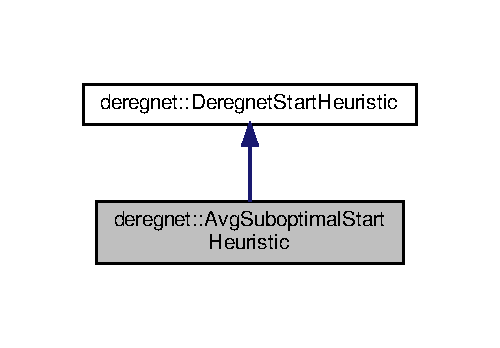
\includegraphics[width=240pt]{classderegnet_1_1AvgSuboptimalStartHeuristic__inherit__graph}
\end{center}
\end{figure}


Collaboration diagram for deregnet\+:\+:Avg\+Suboptimal\+Start\+Heuristic\+:\nopagebreak
\begin{figure}[H]
\begin{center}
\leavevmode
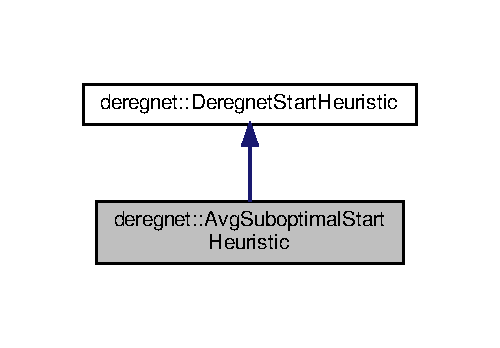
\includegraphics[width=240pt]{classderegnet_1_1AvgSuboptimalStartHeuristic__coll__graph}
\end{center}
\end{figure}
\subsection*{Public Member Functions}
\begin{DoxyCompactItemize}
\item 
\hyperlink{classderegnet_1_1AvgSuboptimalStartHeuristic_a12082995005a50591bb64951417b2a96}{Avg\+Suboptimal\+Start\+Heuristic} (\hyperlink{namespacederegnet_a55b76c55bbabc682cbc61f8b9948799e}{Graph} $\ast$xgraph, \hyperlink{namespacederegnet_ae102b707ae1d6f83c639ece5e0dd5658}{Node\+Map}$<$ double $>$ $\ast$xscore, \hyperlink{namespacederegnet_a744bad34f2de9856d36715a445f027f3}{Node} $\ast$\hyperlink{classderegnet_1_1DeregnetStartHeuristic_a4605d41352e3adf1f9f9f32466a4e61e}{root}, std\+::set$<$ \hyperlink{namespacederegnet_a744bad34f2de9856d36715a445f027f3}{Node} $>$ $\ast$\hyperlink{classderegnet_1_1DeregnetStartHeuristic_aa22c6581cd404bf7ac325850b28dc951}{exclude}, std\+::set$<$ \hyperlink{namespacederegnet_a744bad34f2de9856d36715a445f027f3}{Node} $>$ $\ast$\hyperlink{classderegnet_1_1DeregnetStartHeuristic_ab80c046ff2b7c64086fceb84987b3e50}{receptors}, std\+::function$<$ bool(double, double)$>$ xcmp, \hyperlink{namespacederegnet_ae102b707ae1d6f83c639ece5e0dd5658}{Node\+Map}$<$ std\+::string $>$ $\ast$xnodeid, std\+::set$<$ std\+::string $>$ $\ast$xnodes\+\_\+sof\+\_\+far, double xmax\+\_\+overlap, int xmin\+\_\+size, int xmax\+\_\+size)
\end{DoxyCompactItemize}
\subsection*{Private Member Functions}
\begin{DoxyCompactItemize}
\item 
bool \hyperlink{classderegnet_1_1AvgSuboptimalStartHeuristic_abc4fa54576da31f3037f2c1aa2cd9140}{is\+\_\+overlap\+\_\+node} (\hyperlink{namespacederegnet_a744bad34f2de9856d36715a445f027f3}{Node} $\ast$node)
\item 
virtual \hyperlink{namespacederegnet_a744bad34f2de9856d36715a445f027f3}{Node} $\ast$ \hyperlink{classderegnet_1_1AvgSuboptimalStartHeuristic_a732194c0c56e6f28839114e3ab119109}{get\+\_\+best\+\_\+root} () override
\begin{DoxyCompactList}\small\item\em Find best node to add to solution in every iteration. \end{DoxyCompactList}\item 
virtual bool \hyperlink{classderegnet_1_1AvgSuboptimalStartHeuristic_a668a9db07c0d29c9b3618487f25fe5f4}{search\+\_\+further} () override
\begin{DoxyCompactList}\small\item\em Decide whether to continue searching further (for other solution than the one already found) \end{DoxyCompactList}\item 
virtual bool \hyperlink{classderegnet_1_1AvgSuboptimalStartHeuristic_aca3dd2ae41b88a0bd925b297d490e2cb}{feasible\+\_\+node} (\hyperlink{namespacederegnet_a744bad34f2de9856d36715a445f027f3}{Node} $\ast$node) override
\begin{DoxyCompactList}\small\item\em Decide whether adding a given node to the solution is feasible wrt the given constraints. \end{DoxyCompactList}\item 
double \hyperlink{classderegnet_1_1AvgSuboptimalStartHeuristic_a29659ab4864fddd2c226da7e1ada22ef}{update\+\_\+avg} (\hyperlink{namespacederegnet_a744bad34f2de9856d36715a445f027f3}{Node} $\ast$node)
\end{DoxyCompactItemize}
\subsection*{Private Attributes}
\begin{DoxyCompactItemize}
\item 
\hyperlink{namespacederegnet_ae102b707ae1d6f83c639ece5e0dd5658}{Node\+Map}$<$ std\+::string $>$ $\ast$ \hyperlink{classderegnet_1_1AvgSuboptimalStartHeuristic_af59e6b6ba10fd5d2c210a0947cf37e66}{nodeid}
\item 
std\+::set$<$ std\+::string $>$ $\ast$ \hyperlink{classderegnet_1_1AvgSuboptimalStartHeuristic_ac07c2b61bf03b25e1bd87cb353bd4597}{nodes\+\_\+so\+\_\+far}
\item 
double \hyperlink{classderegnet_1_1AvgSuboptimalStartHeuristic_a6e019ada1557663d456e7f81757d14ab}{max\+\_\+overlap}
\item 
int \hyperlink{classderegnet_1_1AvgSuboptimalStartHeuristic_a71b5a73f79c4c161e9df9085ece2c270}{min\+\_\+size}
\item 
int \hyperlink{classderegnet_1_1AvgSuboptimalStartHeuristic_aafc01553c8d2a9a877f23c6bdee305aa}{max\+\_\+size}
\item 
int \hyperlink{classderegnet_1_1AvgSuboptimalStartHeuristic_ad541b941d327ba928a7951e43ad1fea4}{current\+\_\+overlapping\+\_\+nodes} \{ 0 \}
\item 
double \hyperlink{classderegnet_1_1AvgSuboptimalStartHeuristic_a5c07fde8d2f92daeb4cc33f85e8bf1e2}{current\+\_\+avg} \{ 0.\+0 \}
\end{DoxyCompactItemize}
\subsection*{Additional Inherited Members}


\subsection{Detailed Description}
Implementation of the heuristic solution algorithm for the suboptimal part of the average De\+Reg\+Net algorithm. 

Definition at line 50 of file Avg\+Suboptimal\+Start\+Heuristic.\+hpp.



\subsection{Constructor \& Destructor Documentation}
\mbox{\Hypertarget{classderegnet_1_1AvgSuboptimalStartHeuristic_a12082995005a50591bb64951417b2a96}\label{classderegnet_1_1AvgSuboptimalStartHeuristic_a12082995005a50591bb64951417b2a96}} 
\index{deregnet\+::\+Avg\+Suboptimal\+Start\+Heuristic@{deregnet\+::\+Avg\+Suboptimal\+Start\+Heuristic}!Avg\+Suboptimal\+Start\+Heuristic@{Avg\+Suboptimal\+Start\+Heuristic}}
\index{Avg\+Suboptimal\+Start\+Heuristic@{Avg\+Suboptimal\+Start\+Heuristic}!deregnet\+::\+Avg\+Suboptimal\+Start\+Heuristic@{deregnet\+::\+Avg\+Suboptimal\+Start\+Heuristic}}
\subsubsection{\texorpdfstring{Avg\+Suboptimal\+Start\+Heuristic()}{AvgSuboptimalStartHeuristic()}}
{\footnotesize\ttfamily deregnet\+::\+Avg\+Suboptimal\+Start\+Heuristic\+::\+Avg\+Suboptimal\+Start\+Heuristic (\begin{DoxyParamCaption}\item[{\hyperlink{namespacederegnet_a55b76c55bbabc682cbc61f8b9948799e}{Graph} $\ast$}]{xgraph,  }\item[{\hyperlink{namespacederegnet_ae102b707ae1d6f83c639ece5e0dd5658}{Node\+Map}$<$ double $>$ $\ast$}]{xscore,  }\item[{\hyperlink{namespacederegnet_a744bad34f2de9856d36715a445f027f3}{Node} $\ast$}]{root,  }\item[{std\+::set$<$ \hyperlink{namespacederegnet_a744bad34f2de9856d36715a445f027f3}{Node} $>$ $\ast$}]{exclude,  }\item[{std\+::set$<$ \hyperlink{namespacederegnet_a744bad34f2de9856d36715a445f027f3}{Node} $>$ $\ast$}]{receptors,  }\item[{std\+::function$<$ bool(double, double)$>$}]{xcmp,  }\item[{\hyperlink{namespacederegnet_ae102b707ae1d6f83c639ece5e0dd5658}{Node\+Map}$<$ std\+::string $>$ $\ast$}]{xnodeid,  }\item[{std\+::set$<$ std\+::string $>$ $\ast$}]{xnodes\+\_\+sof\+\_\+far,  }\item[{double}]{xmax\+\_\+overlap,  }\item[{int}]{xmin\+\_\+size,  }\item[{int}]{xmax\+\_\+size }\end{DoxyParamCaption})}



Definition at line 44 of file Avg\+Suboptimal\+Start\+Heuristic.\+cpp.



References max\+\_\+overlap, max\+\_\+size, min\+\_\+size, and nodes\+\_\+so\+\_\+far.


\begin{DoxyCode}
55  : \hyperlink{classderegnet_1_1DeregnetStartHeuristic_af7fa694b10f54c669fce9431214ffc98}{DeregnetStartHeuristic}(xgraph, xscore, \hyperlink{classderegnet_1_1DeregnetStartHeuristic_a4605d41352e3adf1f9f9f32466a4e61e}{root}, 
      \hyperlink{classderegnet_1_1DeregnetStartHeuristic_aa22c6581cd404bf7ac325850b28dc951}{exclude}, \hyperlink{classderegnet_1_1DeregnetStartHeuristic_ab80c046ff2b7c64086fceb84987b3e50}{receptors}, xcmp),
56    \hyperlink{classderegnet_1_1AvgSuboptimalStartHeuristic_af59e6b6ba10fd5d2c210a0947cf37e66}{nodeid} \{ xnodeid \},
57    \hyperlink{classderegnet_1_1AvgSuboptimalStartHeuristic_ac07c2b61bf03b25e1bd87cb353bd4597}{nodes\_so\_far} \{ xnodes\_sof\_far \},
58    \hyperlink{classderegnet_1_1AvgSuboptimalStartHeuristic_a6e019ada1557663d456e7f81757d14ab}{max\_overlap} \{ xmax\_overlap \},
59    \hyperlink{classderegnet_1_1AvgSuboptimalStartHeuristic_a71b5a73f79c4c161e9df9085ece2c270}{min\_size} \{ xmin\_size \},
60    \hyperlink{classderegnet_1_1AvgSuboptimalStartHeuristic_aafc01553c8d2a9a877f23c6bdee305aa}{max\_size} \{ xmax\_size \}
61 \{ \}
\end{DoxyCode}


\subsection{Member Function Documentation}
\mbox{\Hypertarget{classderegnet_1_1AvgSuboptimalStartHeuristic_aca3dd2ae41b88a0bd925b297d490e2cb}\label{classderegnet_1_1AvgSuboptimalStartHeuristic_aca3dd2ae41b88a0bd925b297d490e2cb}} 
\index{deregnet\+::\+Avg\+Suboptimal\+Start\+Heuristic@{deregnet\+::\+Avg\+Suboptimal\+Start\+Heuristic}!feasible\+\_\+node@{feasible\+\_\+node}}
\index{feasible\+\_\+node@{feasible\+\_\+node}!deregnet\+::\+Avg\+Suboptimal\+Start\+Heuristic@{deregnet\+::\+Avg\+Suboptimal\+Start\+Heuristic}}
\subsubsection{\texorpdfstring{feasible\+\_\+node()}{feasible\_node()}}
{\footnotesize\ttfamily bool deregnet\+::\+Avg\+Suboptimal\+Start\+Heuristic\+::feasible\+\_\+node (\begin{DoxyParamCaption}\item[{\hyperlink{namespacederegnet_a744bad34f2de9856d36715a445f027f3}{Node} $\ast$}]{node }\end{DoxyParamCaption})\hspace{0.3cm}{\ttfamily [override]}, {\ttfamily [private]}, {\ttfamily [virtual]}}



Decide whether adding a given node to the solution is feasible wrt the given constraints. 


\begin{DoxyParams}{Parameters}
{\em node} & A node in the graph\\
\hline
\end{DoxyParams}
\begin{DoxyReturn}{Returns}
Whether adding the node is feasible 
\end{DoxyReturn}


Implements \hyperlink{classderegnet_1_1DeregnetStartHeuristic_ac296c4f122f7d3ad2fcc2cbb0d1b5379}{deregnet\+::\+Deregnet\+Start\+Heuristic}.



Definition at line 107 of file Avg\+Suboptimal\+Start\+Heuristic.\+cpp.



References current\+\_\+avg, current\+\_\+overlapping\+\_\+nodes, is\+\_\+overlap\+\_\+node(), max\+\_\+overlap, min\+\_\+size, deregnet\+::\+Deregnet\+Start\+Heuristic\+::start\+\_\+solution, and update\+\_\+avg().


\begin{DoxyCode}
107                                                           \{
108     \textcolor{keywordtype}{double} new\_avg \{ \hyperlink{classderegnet_1_1AvgSuboptimalStartHeuristic_a29659ab4864fddd2c226da7e1ada22ef}{update\_avg}(node) \};
109     \textcolor{keywordtype}{int} current\_size \{ \textcolor{keyword}{static\_cast<}\textcolor{keywordtype}{int}\textcolor{keyword}{>}(\hyperlink{classderegnet_1_1DeregnetStartHeuristic_a7450e11ca0a265b055f95e7832b65e2f}{start\_solution}->size()) \};
110     \textcolor{keywordflow}{if} (new\_avg < current\_avg && current\_size > \hyperlink{classderegnet_1_1AvgSuboptimalStartHeuristic_a71b5a73f79c4c161e9df9085ece2c270}{min\_size})
111         \textcolor{keywordflow}{return} \textcolor{keyword}{false};
112     \hyperlink{classderegnet_1_1AvgSuboptimalStartHeuristic_a5c07fde8d2f92daeb4cc33f85e8bf1e2}{current\_avg} = new\_avg;
113 
114     \textcolor{keywordtype}{bool} overlap\_node \{ \hyperlink{classderegnet_1_1AvgSuboptimalStartHeuristic_abc4fa54576da31f3037f2c1aa2cd9140}{is\_overlap\_node}(node) \};
115     \textcolor{keywordtype}{double} potential\_overlap \{ \textcolor{keyword}{static\_cast<}\textcolor{keywordtype}{double}\textcolor{keyword}{>}( \hyperlink{classderegnet_1_1AvgSuboptimalStartHeuristic_ad541b941d327ba928a7951e43ad1fea4}{current\_overlapping\_nodes} / 
      \hyperlink{classderegnet_1_1DeregnetStartHeuristic_a7450e11ca0a265b055f95e7832b65e2f}{start\_solution}->size() ) \};
116     \textcolor{keywordflow}{if} (\hyperlink{classderegnet_1_1DeregnetStartHeuristic_aa22c6581cd404bf7ac325850b28dc951}{exclude}) \{
117         \textcolor{keywordflow}{if} (overlap\_node) \{
118             \textcolor{keywordflow}{if} (   \hyperlink{classderegnet_1_1DeregnetStartHeuristic_a7450e11ca0a265b055f95e7832b65e2f}{start\_solution}->find(*node) == \hyperlink{classderegnet_1_1DeregnetStartHeuristic_a7450e11ca0a265b055f95e7832b65e2f}{start\_solution}->end()
119                 && potential\_overlap < \hyperlink{classderegnet_1_1AvgSuboptimalStartHeuristic_a6e019ada1557663d456e7f81757d14ab}{max\_overlap}
120                 && \hyperlink{classderegnet_1_1DeregnetStartHeuristic_aa22c6581cd404bf7ac325850b28dc951}{exclude}->find(*node) == \hyperlink{classderegnet_1_1DeregnetStartHeuristic_aa22c6581cd404bf7ac325850b28dc951}{exclude}->end()) \{
121                 \hyperlink{classderegnet_1_1AvgSuboptimalStartHeuristic_ad541b941d327ba928a7951e43ad1fea4}{current\_overlapping\_nodes}++;
122                 \textcolor{keywordflow}{return} \textcolor{keyword}{true};
123             \}
124         \}
125         \textcolor{keywordflow}{else} \{
126             \textcolor{keywordflow}{if} (\hyperlink{classderegnet_1_1DeregnetStartHeuristic_a7450e11ca0a265b055f95e7832b65e2f}{start\_solution}->find(*node) == \hyperlink{classderegnet_1_1DeregnetStartHeuristic_a7450e11ca0a265b055f95e7832b65e2f}{start\_solution}->end() && 
      \hyperlink{classderegnet_1_1DeregnetStartHeuristic_aa22c6581cd404bf7ac325850b28dc951}{exclude}->find(*node) == \hyperlink{classderegnet_1_1DeregnetStartHeuristic_aa22c6581cd404bf7ac325850b28dc951}{exclude}->end())
127                 \textcolor{keywordflow}{return} \textcolor{keyword}{true};
128         \}
129     \}
130     \textcolor{keywordflow}{else} \{
131         \textcolor{keywordflow}{if} (overlap\_node) \{
132             \textcolor{keywordflow}{if} (   \hyperlink{classderegnet_1_1DeregnetStartHeuristic_a7450e11ca0a265b055f95e7832b65e2f}{start\_solution}->find(*node) == \hyperlink{classderegnet_1_1DeregnetStartHeuristic_a7450e11ca0a265b055f95e7832b65e2f}{start\_solution}->end()
133                 && potential\_overlap < \hyperlink{classderegnet_1_1AvgSuboptimalStartHeuristic_a6e019ada1557663d456e7f81757d14ab}{max\_overlap}) \{
134                 \hyperlink{classderegnet_1_1AvgSuboptimalStartHeuristic_ad541b941d327ba928a7951e43ad1fea4}{current\_overlapping\_nodes}++;
135                 \textcolor{keywordflow}{return} \textcolor{keyword}{true};
136             \}
137         \}
138         \textcolor{keywordflow}{else} \{
139             \textcolor{keywordflow}{if} (\hyperlink{classderegnet_1_1DeregnetStartHeuristic_a7450e11ca0a265b055f95e7832b65e2f}{start\_solution}->find(*node) == \hyperlink{classderegnet_1_1DeregnetStartHeuristic_a7450e11ca0a265b055f95e7832b65e2f}{start\_solution}->end())
140                 \textcolor{keywordflow}{return} \textcolor{keyword}{true};
141         \}
142     \}
143     \textcolor{keywordflow}{return} \textcolor{keyword}{false};
144 \}
\end{DoxyCode}
Here is the call graph for this function\+:\nopagebreak
\begin{figure}[H]
\begin{center}
\leavevmode
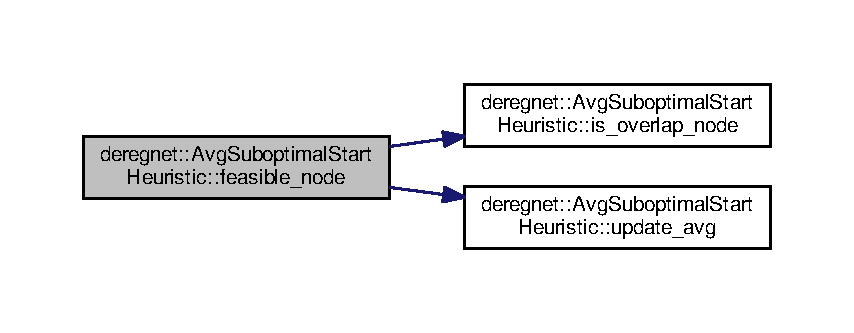
\includegraphics[width=350pt]{classderegnet_1_1AvgSuboptimalStartHeuristic_aca3dd2ae41b88a0bd925b297d490e2cb_cgraph}
\end{center}
\end{figure}
\mbox{\Hypertarget{classderegnet_1_1AvgSuboptimalStartHeuristic_a732194c0c56e6f28839114e3ab119109}\label{classderegnet_1_1AvgSuboptimalStartHeuristic_a732194c0c56e6f28839114e3ab119109}} 
\index{deregnet\+::\+Avg\+Suboptimal\+Start\+Heuristic@{deregnet\+::\+Avg\+Suboptimal\+Start\+Heuristic}!get\+\_\+best\+\_\+root@{get\+\_\+best\+\_\+root}}
\index{get\+\_\+best\+\_\+root@{get\+\_\+best\+\_\+root}!deregnet\+::\+Avg\+Suboptimal\+Start\+Heuristic@{deregnet\+::\+Avg\+Suboptimal\+Start\+Heuristic}}
\subsubsection{\texorpdfstring{get\+\_\+best\+\_\+root()}{get\_best\_root()}}
{\footnotesize\ttfamily \hyperlink{namespacederegnet_a744bad34f2de9856d36715a445f027f3}{Node} $\ast$ deregnet\+::\+Avg\+Suboptimal\+Start\+Heuristic\+::get\+\_\+best\+\_\+root (\begin{DoxyParamCaption}{ }\end{DoxyParamCaption})\hspace{0.3cm}{\ttfamily [override]}, {\ttfamily [private]}, {\ttfamily [virtual]}}



Find best node to add to solution in every iteration. 

\begin{DoxyReturn}{Returns}
The best node to add 
\end{DoxyReturn}


Implements \hyperlink{classderegnet_1_1DeregnetStartHeuristic_a372be86d0fb8ac94bd926a1f4d09e102}{deregnet\+::\+Deregnet\+Start\+Heuristic}.



Definition at line 63 of file Avg\+Suboptimal\+Start\+Heuristic.\+cpp.



References deregnet\+::\+Deregnet\+Start\+Heuristic\+::graph, I\+N\+V\+A\+L\+ID, is\+\_\+overlap\+\_\+node(), max\+\_\+overlap, nodes\+\_\+so\+\_\+far, and deregnet\+::\+Deregnet\+Start\+Heuristic\+::update\+\_\+best\+\_\+node().


\begin{DoxyCode}
63                                                  \{
64     \textcolor{keywordtype}{double} best;
65     \hyperlink{namespacederegnet_a744bad34f2de9856d36715a445f027f3}{Node}* best\_node \{ \textcolor{keyword}{nullptr} \};
66     \textcolor{keywordtype}{bool} overlap\_matters \{ \hyperlink{classderegnet_1_1AvgSuboptimalStartHeuristic_a6e019ada1557663d456e7f81757d14ab}{max\_overlap} < 1.0 / \hyperlink{classderegnet_1_1AvgSuboptimalStartHeuristic_ac07c2b61bf03b25e1bd87cb353bd4597}{nodes\_so\_far}->size() \};
67     \textcolor{keywordflow}{if} (\hyperlink{classderegnet_1_1DeregnetStartHeuristic_ab80c046ff2b7c64086fceb84987b3e50}{receptors})
68         \textcolor{keywordflow}{for} (\textcolor{keyword}{auto} v : *\hyperlink{classderegnet_1_1DeregnetStartHeuristic_ab80c046ff2b7c64086fceb84987b3e50}{receptors}) \{
69             \textcolor{keywordflow}{if} ( \hyperlink{classderegnet_1_1AvgSuboptimalStartHeuristic_abc4fa54576da31f3037f2c1aa2cd9140}{is\_overlap\_node}(&v) && overlap\_matters )
70                 \textcolor{keywordflow}{continue};
71             \textcolor{keywordflow}{else}
72                 \hyperlink{classderegnet_1_1DeregnetStartHeuristic_a50179ff9db4d416b93ff41d1dcee1358}{update\_best\_node}(&best\_node, &v, &best);
73         \}
74     \textcolor{keywordflow}{else}
75         \textcolor{keywordflow}{for} (\hyperlink{namespacederegnet_ac34314e1b5f456fc6d1bb9d96316de4a}{NodeIt} v(*\hyperlink{classderegnet_1_1DeregnetStartHeuristic_a4da8e53fc7c0fa3dbe0e3ef07296d75e}{graph}); v != \hyperlink{usinglemon_8hpp_adf770fe2eec438e3758ffe905dbae208}{INVALID}; ++v) \{
76             \textcolor{keywordflow}{if} ( \hyperlink{classderegnet_1_1AvgSuboptimalStartHeuristic_abc4fa54576da31f3037f2c1aa2cd9140}{is\_overlap\_node}(&v) && overlap\_matters )
77                 \textcolor{keywordflow}{continue};
78             \textcolor{keywordflow}{else}
79                 \hyperlink{classderegnet_1_1DeregnetStartHeuristic_a50179ff9db4d416b93ff41d1dcee1358}{update\_best\_node}(&best\_node, &v, &best);
80         \}
81     \textcolor{keywordflow}{return} best\_node;
82 \}
\end{DoxyCode}
Here is the call graph for this function\+:\nopagebreak
\begin{figure}[H]
\begin{center}
\leavevmode
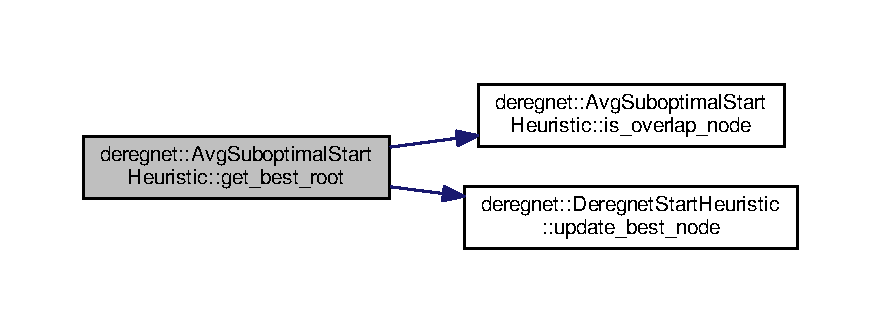
\includegraphics[width=350pt]{classderegnet_1_1AvgSuboptimalStartHeuristic_a732194c0c56e6f28839114e3ab119109_cgraph}
\end{center}
\end{figure}
\mbox{\Hypertarget{classderegnet_1_1AvgSuboptimalStartHeuristic_abc4fa54576da31f3037f2c1aa2cd9140}\label{classderegnet_1_1AvgSuboptimalStartHeuristic_abc4fa54576da31f3037f2c1aa2cd9140}} 
\index{deregnet\+::\+Avg\+Suboptimal\+Start\+Heuristic@{deregnet\+::\+Avg\+Suboptimal\+Start\+Heuristic}!is\+\_\+overlap\+\_\+node@{is\+\_\+overlap\+\_\+node}}
\index{is\+\_\+overlap\+\_\+node@{is\+\_\+overlap\+\_\+node}!deregnet\+::\+Avg\+Suboptimal\+Start\+Heuristic@{deregnet\+::\+Avg\+Suboptimal\+Start\+Heuristic}}
\subsubsection{\texorpdfstring{is\+\_\+overlap\+\_\+node()}{is\_overlap\_node()}}
{\footnotesize\ttfamily bool deregnet\+::\+Avg\+Suboptimal\+Start\+Heuristic\+::is\+\_\+overlap\+\_\+node (\begin{DoxyParamCaption}\item[{\hyperlink{namespacederegnet_a744bad34f2de9856d36715a445f027f3}{Node} $\ast$}]{node }\end{DoxyParamCaption})\hspace{0.3cm}{\ttfamily [private]}}



Definition at line 146 of file Avg\+Suboptimal\+Start\+Heuristic.\+cpp.



References nodeid, and nodes\+\_\+so\+\_\+far.



Referenced by feasible\+\_\+node(), and get\+\_\+best\+\_\+root().


\begin{DoxyCode}
146                                                             \{
147     \textcolor{keywordflow}{for} (set<string>::iterator nodeID = \hyperlink{classderegnet_1_1AvgSuboptimalStartHeuristic_ac07c2b61bf03b25e1bd87cb353bd4597}{nodes\_so\_far}->begin(); nodeID != 
      \hyperlink{classderegnet_1_1AvgSuboptimalStartHeuristic_ac07c2b61bf03b25e1bd87cb353bd4597}{nodes\_so\_far}->end(); ++nodeID)
148         \textcolor{keywordflow}{if} ( *nodeID == (*\hyperlink{classderegnet_1_1AvgSuboptimalStartHeuristic_af59e6b6ba10fd5d2c210a0947cf37e66}{nodeid})[*node] )
149             \textcolor{keywordflow}{return} \textcolor{keyword}{true};
150     \textcolor{keywordflow}{return} \textcolor{keyword}{false};
151 \}
\end{DoxyCode}
Here is the caller graph for this function\+:\nopagebreak
\begin{figure}[H]
\begin{center}
\leavevmode
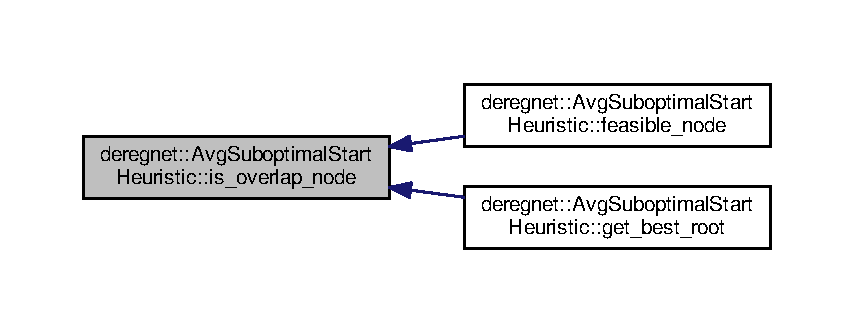
\includegraphics[width=350pt]{classderegnet_1_1AvgSuboptimalStartHeuristic_abc4fa54576da31f3037f2c1aa2cd9140_icgraph}
\end{center}
\end{figure}
\mbox{\Hypertarget{classderegnet_1_1AvgSuboptimalStartHeuristic_a668a9db07c0d29c9b3618487f25fe5f4}\label{classderegnet_1_1AvgSuboptimalStartHeuristic_a668a9db07c0d29c9b3618487f25fe5f4}} 
\index{deregnet\+::\+Avg\+Suboptimal\+Start\+Heuristic@{deregnet\+::\+Avg\+Suboptimal\+Start\+Heuristic}!search\+\_\+further@{search\+\_\+further}}
\index{search\+\_\+further@{search\+\_\+further}!deregnet\+::\+Avg\+Suboptimal\+Start\+Heuristic@{deregnet\+::\+Avg\+Suboptimal\+Start\+Heuristic}}
\subsubsection{\texorpdfstring{search\+\_\+further()}{search\_further()}}
{\footnotesize\ttfamily bool deregnet\+::\+Avg\+Suboptimal\+Start\+Heuristic\+::search\+\_\+further (\begin{DoxyParamCaption}{ }\end{DoxyParamCaption})\hspace{0.3cm}{\ttfamily [override]}, {\ttfamily [private]}, {\ttfamily [virtual]}}



Decide whether to continue searching further (for other solution than the one already found) 

\begin{DoxyReturn}{Returns}
Whether to search further 
\end{DoxyReturn}


Implements \hyperlink{classderegnet_1_1DeregnetStartHeuristic_ac3ee2c3022512f9d4ec7a6b49358e60a}{deregnet\+::\+Deregnet\+Start\+Heuristic}.



Definition at line 84 of file Avg\+Suboptimal\+Start\+Heuristic.\+cpp.



References deregnet\+::\+Deregnet\+Start\+Heuristic\+::found\+\_\+node, max\+\_\+size, min\+\_\+size, deregnet\+::\+Deregnet\+Start\+Heuristic\+::start\+\_\+solution, and deregnet\+::\+Deregnet\+Start\+Heuristic\+::success.


\begin{DoxyCode}
84                                                  \{
85     \textcolor{keywordtype}{int} current\_size \{ \textcolor{keyword}{static\_cast<}\textcolor{keywordtype}{int}\textcolor{keyword}{>}(\hyperlink{classderegnet_1_1DeregnetStartHeuristic_a7450e11ca0a265b055f95e7832b65e2f}{start\_solution}->size()) \};
86     \textcolor{keywordflow}{if} (current\_size < \hyperlink{classderegnet_1_1AvgSuboptimalStartHeuristic_a71b5a73f79c4c161e9df9085ece2c270}{min\_size}) \{
87         \textcolor{keywordflow}{if} (\hyperlink{classderegnet_1_1DeregnetStartHeuristic_a1ca705794583fb3b6e563efeceb4445e}{found\_node})
88             \textcolor{keywordflow}{return} \textcolor{keyword}{true};
89         \textcolor{keywordflow}{else}
90             \textcolor{keywordflow}{return} \textcolor{keyword}{false};
91     \}
92     \textcolor{keywordflow}{if} (current\_size >= \hyperlink{classderegnet_1_1AvgSuboptimalStartHeuristic_a71b5a73f79c4c161e9df9085ece2c270}{min\_size} && current\_size < \hyperlink{classderegnet_1_1AvgSuboptimalStartHeuristic_aafc01553c8d2a9a877f23c6bdee305aa}{max\_size}) \{
93         \textcolor{keywordflow}{if} (\hyperlink{classderegnet_1_1DeregnetStartHeuristic_a1ca705794583fb3b6e563efeceb4445e}{found\_node})
94             \textcolor{keywordflow}{return} \textcolor{keyword}{true};
95         \textcolor{keywordflow}{else} \{
96             \hyperlink{classderegnet_1_1DeregnetStartHeuristic_a72fd16ee027f6aa973f1ff29746addba}{success} = \textcolor{keyword}{true};
97             \textcolor{keywordflow}{return} \textcolor{keyword}{false};
98         \}
99     \}
100     \textcolor{keywordflow}{if} (current\_size == \hyperlink{classderegnet_1_1AvgSuboptimalStartHeuristic_aafc01553c8d2a9a877f23c6bdee305aa}{max\_size}) \{
101         \hyperlink{classderegnet_1_1DeregnetStartHeuristic_a72fd16ee027f6aa973f1ff29746addba}{success} = \textcolor{keyword}{true};
102         \textcolor{keywordflow}{return} \textcolor{keyword}{false};
103     \}
104     \textcolor{keywordflow}{return} \textcolor{keyword}{false};
105 \}
\end{DoxyCode}
\mbox{\Hypertarget{classderegnet_1_1AvgSuboptimalStartHeuristic_a29659ab4864fddd2c226da7e1ada22ef}\label{classderegnet_1_1AvgSuboptimalStartHeuristic_a29659ab4864fddd2c226da7e1ada22ef}} 
\index{deregnet\+::\+Avg\+Suboptimal\+Start\+Heuristic@{deregnet\+::\+Avg\+Suboptimal\+Start\+Heuristic}!update\+\_\+avg@{update\+\_\+avg}}
\index{update\+\_\+avg@{update\+\_\+avg}!deregnet\+::\+Avg\+Suboptimal\+Start\+Heuristic@{deregnet\+::\+Avg\+Suboptimal\+Start\+Heuristic}}
\subsubsection{\texorpdfstring{update\+\_\+avg()}{update\_avg()}}
{\footnotesize\ttfamily double deregnet\+::\+Avg\+Suboptimal\+Start\+Heuristic\+::update\+\_\+avg (\begin{DoxyParamCaption}\item[{\hyperlink{namespacederegnet_a744bad34f2de9856d36715a445f027f3}{Node} $\ast$}]{node }\end{DoxyParamCaption})\hspace{0.3cm}{\ttfamily [private]}}



Definition at line 153 of file Avg\+Suboptimal\+Start\+Heuristic.\+cpp.



References current\+\_\+avg, deregnet\+::\+Deregnet\+Start\+Heuristic\+::score, and deregnet\+::\+Deregnet\+Start\+Heuristic\+::start\+\_\+solution.



Referenced by feasible\+\_\+node().


\begin{DoxyCode}
153                                                          \{
154     \textcolor{keywordtype}{int} current\_size \{ \textcolor{keyword}{static\_cast<}\textcolor{keywordtype}{int}\textcolor{keyword}{>}(\hyperlink{classderegnet_1_1DeregnetStartHeuristic_a7450e11ca0a265b055f95e7832b65e2f}{start\_solution}->size()) \};
155     \textcolor{keywordflow}{return} ((*\hyperlink{classderegnet_1_1DeregnetStartHeuristic_ae03300e79482975e98f95cba19ad32b0}{score})[*node] + current\_size * \hyperlink{classderegnet_1_1AvgSuboptimalStartHeuristic_a5c07fde8d2f92daeb4cc33f85e8bf1e2}{current\_avg}) / (current\_size + 1);
156 \}
\end{DoxyCode}
Here is the caller graph for this function\+:\nopagebreak
\begin{figure}[H]
\begin{center}
\leavevmode
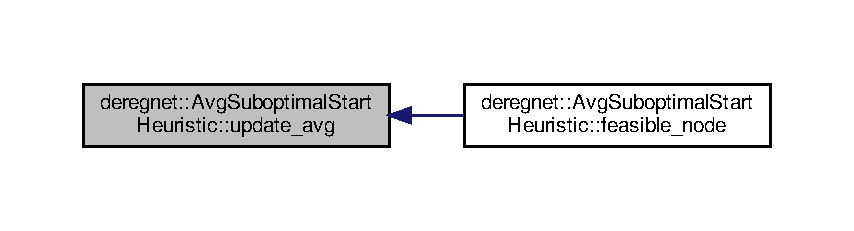
\includegraphics[width=350pt]{classderegnet_1_1AvgSuboptimalStartHeuristic_a29659ab4864fddd2c226da7e1ada22ef_icgraph}
\end{center}
\end{figure}


\subsection{Member Data Documentation}
\mbox{\Hypertarget{classderegnet_1_1AvgSuboptimalStartHeuristic_a5c07fde8d2f92daeb4cc33f85e8bf1e2}\label{classderegnet_1_1AvgSuboptimalStartHeuristic_a5c07fde8d2f92daeb4cc33f85e8bf1e2}} 
\index{deregnet\+::\+Avg\+Suboptimal\+Start\+Heuristic@{deregnet\+::\+Avg\+Suboptimal\+Start\+Heuristic}!current\+\_\+avg@{current\+\_\+avg}}
\index{current\+\_\+avg@{current\+\_\+avg}!deregnet\+::\+Avg\+Suboptimal\+Start\+Heuristic@{deregnet\+::\+Avg\+Suboptimal\+Start\+Heuristic}}
\subsubsection{\texorpdfstring{current\+\_\+avg}{current\_avg}}
{\footnotesize\ttfamily double deregnet\+::\+Avg\+Suboptimal\+Start\+Heuristic\+::current\+\_\+avg \{ 0.\+0 \}\hspace{0.3cm}{\ttfamily [private]}}



Definition at line 60 of file Avg\+Suboptimal\+Start\+Heuristic.\+hpp.



Referenced by feasible\+\_\+node(), and update\+\_\+avg().

\mbox{\Hypertarget{classderegnet_1_1AvgSuboptimalStartHeuristic_ad541b941d327ba928a7951e43ad1fea4}\label{classderegnet_1_1AvgSuboptimalStartHeuristic_ad541b941d327ba928a7951e43ad1fea4}} 
\index{deregnet\+::\+Avg\+Suboptimal\+Start\+Heuristic@{deregnet\+::\+Avg\+Suboptimal\+Start\+Heuristic}!current\+\_\+overlapping\+\_\+nodes@{current\+\_\+overlapping\+\_\+nodes}}
\index{current\+\_\+overlapping\+\_\+nodes@{current\+\_\+overlapping\+\_\+nodes}!deregnet\+::\+Avg\+Suboptimal\+Start\+Heuristic@{deregnet\+::\+Avg\+Suboptimal\+Start\+Heuristic}}
\subsubsection{\texorpdfstring{current\+\_\+overlapping\+\_\+nodes}{current\_overlapping\_nodes}}
{\footnotesize\ttfamily int deregnet\+::\+Avg\+Suboptimal\+Start\+Heuristic\+::current\+\_\+overlapping\+\_\+nodes \{ 0 \}\hspace{0.3cm}{\ttfamily [private]}}



Definition at line 59 of file Avg\+Suboptimal\+Start\+Heuristic.\+hpp.



Referenced by feasible\+\_\+node().

\mbox{\Hypertarget{classderegnet_1_1AvgSuboptimalStartHeuristic_a6e019ada1557663d456e7f81757d14ab}\label{classderegnet_1_1AvgSuboptimalStartHeuristic_a6e019ada1557663d456e7f81757d14ab}} 
\index{deregnet\+::\+Avg\+Suboptimal\+Start\+Heuristic@{deregnet\+::\+Avg\+Suboptimal\+Start\+Heuristic}!max\+\_\+overlap@{max\+\_\+overlap}}
\index{max\+\_\+overlap@{max\+\_\+overlap}!deregnet\+::\+Avg\+Suboptimal\+Start\+Heuristic@{deregnet\+::\+Avg\+Suboptimal\+Start\+Heuristic}}
\subsubsection{\texorpdfstring{max\+\_\+overlap}{max\_overlap}}
{\footnotesize\ttfamily double deregnet\+::\+Avg\+Suboptimal\+Start\+Heuristic\+::max\+\_\+overlap\hspace{0.3cm}{\ttfamily [private]}}



Definition at line 56 of file Avg\+Suboptimal\+Start\+Heuristic.\+hpp.



Referenced by Avg\+Suboptimal\+Start\+Heuristic(), feasible\+\_\+node(), and get\+\_\+best\+\_\+root().

\mbox{\Hypertarget{classderegnet_1_1AvgSuboptimalStartHeuristic_aafc01553c8d2a9a877f23c6bdee305aa}\label{classderegnet_1_1AvgSuboptimalStartHeuristic_aafc01553c8d2a9a877f23c6bdee305aa}} 
\index{deregnet\+::\+Avg\+Suboptimal\+Start\+Heuristic@{deregnet\+::\+Avg\+Suboptimal\+Start\+Heuristic}!max\+\_\+size@{max\+\_\+size}}
\index{max\+\_\+size@{max\+\_\+size}!deregnet\+::\+Avg\+Suboptimal\+Start\+Heuristic@{deregnet\+::\+Avg\+Suboptimal\+Start\+Heuristic}}
\subsubsection{\texorpdfstring{max\+\_\+size}{max\_size}}
{\footnotesize\ttfamily int deregnet\+::\+Avg\+Suboptimal\+Start\+Heuristic\+::max\+\_\+size\hspace{0.3cm}{\ttfamily [private]}}



Definition at line 58 of file Avg\+Suboptimal\+Start\+Heuristic.\+hpp.



Referenced by Avg\+Suboptimal\+Start\+Heuristic(), and search\+\_\+further().

\mbox{\Hypertarget{classderegnet_1_1AvgSuboptimalStartHeuristic_a71b5a73f79c4c161e9df9085ece2c270}\label{classderegnet_1_1AvgSuboptimalStartHeuristic_a71b5a73f79c4c161e9df9085ece2c270}} 
\index{deregnet\+::\+Avg\+Suboptimal\+Start\+Heuristic@{deregnet\+::\+Avg\+Suboptimal\+Start\+Heuristic}!min\+\_\+size@{min\+\_\+size}}
\index{min\+\_\+size@{min\+\_\+size}!deregnet\+::\+Avg\+Suboptimal\+Start\+Heuristic@{deregnet\+::\+Avg\+Suboptimal\+Start\+Heuristic}}
\subsubsection{\texorpdfstring{min\+\_\+size}{min\_size}}
{\footnotesize\ttfamily int deregnet\+::\+Avg\+Suboptimal\+Start\+Heuristic\+::min\+\_\+size\hspace{0.3cm}{\ttfamily [private]}}



Definition at line 57 of file Avg\+Suboptimal\+Start\+Heuristic.\+hpp.



Referenced by Avg\+Suboptimal\+Start\+Heuristic(), feasible\+\_\+node(), and search\+\_\+further().

\mbox{\Hypertarget{classderegnet_1_1AvgSuboptimalStartHeuristic_af59e6b6ba10fd5d2c210a0947cf37e66}\label{classderegnet_1_1AvgSuboptimalStartHeuristic_af59e6b6ba10fd5d2c210a0947cf37e66}} 
\index{deregnet\+::\+Avg\+Suboptimal\+Start\+Heuristic@{deregnet\+::\+Avg\+Suboptimal\+Start\+Heuristic}!nodeid@{nodeid}}
\index{nodeid@{nodeid}!deregnet\+::\+Avg\+Suboptimal\+Start\+Heuristic@{deregnet\+::\+Avg\+Suboptimal\+Start\+Heuristic}}
\subsubsection{\texorpdfstring{nodeid}{nodeid}}
{\footnotesize\ttfamily \hyperlink{namespacederegnet_ae102b707ae1d6f83c639ece5e0dd5658}{Node\+Map}$<$std\+::string$>$$\ast$ deregnet\+::\+Avg\+Suboptimal\+Start\+Heuristic\+::nodeid\hspace{0.3cm}{\ttfamily [private]}}



Definition at line 54 of file Avg\+Suboptimal\+Start\+Heuristic.\+hpp.



Referenced by is\+\_\+overlap\+\_\+node().

\mbox{\Hypertarget{classderegnet_1_1AvgSuboptimalStartHeuristic_ac07c2b61bf03b25e1bd87cb353bd4597}\label{classderegnet_1_1AvgSuboptimalStartHeuristic_ac07c2b61bf03b25e1bd87cb353bd4597}} 
\index{deregnet\+::\+Avg\+Suboptimal\+Start\+Heuristic@{deregnet\+::\+Avg\+Suboptimal\+Start\+Heuristic}!nodes\+\_\+so\+\_\+far@{nodes\+\_\+so\+\_\+far}}
\index{nodes\+\_\+so\+\_\+far@{nodes\+\_\+so\+\_\+far}!deregnet\+::\+Avg\+Suboptimal\+Start\+Heuristic@{deregnet\+::\+Avg\+Suboptimal\+Start\+Heuristic}}
\subsubsection{\texorpdfstring{nodes\+\_\+so\+\_\+far}{nodes\_so\_far}}
{\footnotesize\ttfamily std\+::set$<$std\+::string$>$$\ast$ deregnet\+::\+Avg\+Suboptimal\+Start\+Heuristic\+::nodes\+\_\+so\+\_\+far\hspace{0.3cm}{\ttfamily [private]}}



Definition at line 55 of file Avg\+Suboptimal\+Start\+Heuristic.\+hpp.



Referenced by Avg\+Suboptimal\+Start\+Heuristic(), get\+\_\+best\+\_\+root(), and is\+\_\+overlap\+\_\+node().



The documentation for this class was generated from the following files\+:\begin{DoxyCompactItemize}
\item 
/datadisk/bbubu/home/self/bbubu/projects/deregnet/src/\hyperlink{AvgSuboptimalStartHeuristic_8hpp}{Avg\+Suboptimal\+Start\+Heuristic.\+hpp}\item 
/datadisk/bbubu/home/self/bbubu/projects/deregnet/src/\hyperlink{AvgSuboptimalStartHeuristic_8cpp}{Avg\+Suboptimal\+Start\+Heuristic.\+cpp}\end{DoxyCompactItemize}

\hypertarget{classderegnet_1_1DeregnetData}{}\section{deregnet\+:\+:Deregnet\+Data Class Reference}
\label{classderegnet_1_1DeregnetData}\index{deregnet\+::\+Deregnet\+Data@{deregnet\+::\+Deregnet\+Data}}


Represents all shared parameters and data needed to run a De\+Reg\+Net algorithm.  




{\ttfamily \#include $<$Deregnet\+Data.\+hpp$>$}



Inheritance diagram for deregnet\+:\+:Deregnet\+Data\+:\nopagebreak
\begin{figure}[H]
\begin{center}
\leavevmode
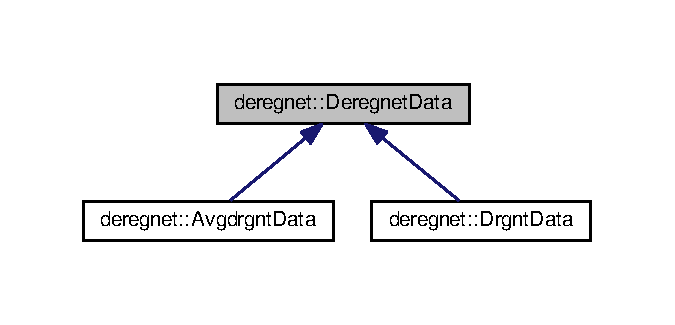
\includegraphics[width=324pt]{classderegnet_1_1DeregnetData__inherit__graph}
\end{center}
\end{figure}
\subsection*{Public Member Functions}
\begin{DoxyCompactItemize}
\item 
void \hyperlink{classderegnet_1_1DeregnetData_ae5edd8f077b20056f416d42ef3fb03d2}{read\+\_\+graph} (std\+::string $\ast$path\+To\+Lgf)
\begin{DoxyCompactList}\small\item\em Read graph from L\+GF (Lemon Graph Format) file. \end{DoxyCompactList}\item 
void \hyperlink{classderegnet_1_1DeregnetData_a01308048556370738e4ac335aba62ffd}{read\+\_\+score} (std\+::string $\ast$path\+To\+Tsv, bool take\+\_\+abs)
\begin{DoxyCompactList}\small\item\em Read scores from file. \end{DoxyCompactList}\item 
void \hyperlink{classderegnet_1_1DeregnetData_a7d662c0dd84d814bbaaf56718a99306a}{get\+\_\+node\+\_\+set} (std\+::set$<$ \hyperlink{namespacederegnet_a744bad34f2de9856d36715a445f027f3}{Node} $>$ $\ast$$\ast$node\+\_\+set, std\+::set$<$ std\+::string $>$ $\ast$node\+\_\+ids)
\begin{DoxyCompactList}\small\item\em Translate a set of node id\textquotesingle{}s into a set of (Lemon) nodes. \end{DoxyCompactList}\item 
void \hyperlink{classderegnet_1_1DeregnetData_aaef262d5ca460f10851b25c01ad2f9bc}{get\+\_\+root} (std\+::string $\ast$root\+\_\+id)
\begin{DoxyCompactList}\small\item\em Get (Lemon) node corresponding to the id of the root. \end{DoxyCompactList}\end{DoxyCompactItemize}
\subsection*{Public Attributes}
\begin{DoxyCompactItemize}
\item 
\hyperlink{namespacederegnet_a55b76c55bbabc682cbc61f8b9948799e}{Graph} $\ast$ \hyperlink{classderegnet_1_1DeregnetData_ab76d30fa2ef87099faecb31e3f95b6d6}{graph} \{ nullptr \}
\begin{DoxyCompactList}\small\item\em Actual graph used to run the algorithms. \end{DoxyCompactList}\item 
\hyperlink{namespacederegnet_a55b76c55bbabc682cbc61f8b9948799e}{Graph} $\ast$ \hyperlink{classderegnet_1_1DeregnetData_a3ea2abe9900785d80fa0141afdd985a9}{original\+\_\+graph} \{ nullptr \}
\begin{DoxyCompactList}\small\item\em Original input graph. \end{DoxyCompactList}\item 
\hyperlink{namespacederegnet_ae102b707ae1d6f83c639ece5e0dd5658}{Node\+Map}$<$ double $>$ $\ast$ \hyperlink{classderegnet_1_1DeregnetData_a32970c8f43eb8be313ad08d829223b1f}{score} \{ nullptr \}
\begin{DoxyCompactList}\small\item\em Node scores. \end{DoxyCompactList}\item 
\hyperlink{namespacederegnet_ae102b707ae1d6f83c639ece5e0dd5658}{Node\+Map}$<$ std\+::string $>$ $\ast$ \hyperlink{classderegnet_1_1DeregnetData_a3b57d7ed19c104c7fe257e17f0d2cfb5}{nodeid} \{ nullptr \}
\begin{DoxyCompactList}\small\item\em Node id\textquotesingle{}s. \end{DoxyCompactList}\item 
\hyperlink{namespacederegnet_a744bad34f2de9856d36715a445f027f3}{Node} $\ast$ \hyperlink{classderegnet_1_1DeregnetData_a51a22fd88f929b1b1a00edb409b4cd55}{root} \{ nullptr \}
\begin{DoxyCompactList}\small\item\em Root node (null if the algorithm is supposed to find the root) \end{DoxyCompactList}\item 
std\+::set$<$ \hyperlink{namespacederegnet_a744bad34f2de9856d36715a445f027f3}{Node} $>$ $\ast$ \hyperlink{classderegnet_1_1DeregnetData_a1fe559c6056cd411647f836849e4b0da}{terminals} \{ nullptr \}
\begin{DoxyCompactList}\small\item\em Nodes classified as \textquotesingle{}terminals\textquotesingle{}. \end{DoxyCompactList}\item 
std\+::set$<$ \hyperlink{namespacederegnet_a744bad34f2de9856d36715a445f027f3}{Node} $>$ $\ast$ \hyperlink{classderegnet_1_1DeregnetData_a470cc9f84741c59897ab1e7a3daa1205}{receptors} \{ nullptr \}
\begin{DoxyCompactList}\small\item\em Nodes classified as \textquotesingle{}receptors\textquotesingle{}. \end{DoxyCompactList}\item 
std\+::set$<$ \hyperlink{namespacederegnet_a744bad34f2de9856d36715a445f027f3}{Node} $>$ $\ast$ \hyperlink{classderegnet_1_1DeregnetData_a438d16e60be5d119d174aa039f070ab2}{include} \{ nullptr \}
\begin{DoxyCompactList}\small\item\em Nodes included in any subgraph a priori. \end{DoxyCompactList}\item 
std\+::set$<$ \hyperlink{namespacederegnet_a744bad34f2de9856d36715a445f027f3}{Node} $>$ $\ast$ \hyperlink{classderegnet_1_1DeregnetData_a8e4398e6ece11ef87767914c6f2c304d}{exclude} \{ nullptr \}
\begin{DoxyCompactList}\small\item\em Nodes excluded from any subgraph a priori. \end{DoxyCompactList}\item 
int \hyperlink{classderegnet_1_1DeregnetData_adb7428cd99112156ae9f80187af9ebbe}{num\+\_\+subopt\+\_\+iter} \{ 0 \}
\begin{DoxyCompactList}\small\item\em Number of iterations to find suboptimal subgraphs. \end{DoxyCompactList}\item 
double \hyperlink{classderegnet_1_1DeregnetData_a43111d8664fd9db36f36f75b24ba62e9}{max\+\_\+overlap} \{ 0.\+0 \}
\begin{DoxyCompactList}\small\item\em Maximal percentage of overlap to previous subgraphs when searching for suboptimal subgraphs. \end{DoxyCompactList}\item 
double $\ast$ \hyperlink{classderegnet_1_1DeregnetData_ac378faf7e8466135b8dc0ced907d98ae}{time\+\_\+limit} \{ nullptr \}
\begin{DoxyCompactList}\small\item\em Time limit of a single solve. \end{DoxyCompactList}\item 
double $\ast$ \hyperlink{classderegnet_1_1DeregnetData_a3637c87366454adc152487fc2f5cfede}{gap\+\_\+cut} \{ nullptr \}
\begin{DoxyCompactList}\small\item\em Gap tolerance. \end{DoxyCompactList}\item 
bool \hyperlink{classderegnet_1_1DeregnetData_ae7936fe59661a68464134b9251303727}{receptor\+\_\+as\+\_\+root} \{ true \}
\begin{DoxyCompactList}\small\item\em Whether to orient the subgraphs such that the root acts as \textquotesingle{}receptor\textquotesingle{}. \end{DoxyCompactList}\item 
std\+::string \hyperlink{classderegnet_1_1DeregnetData_ac3918536b5423facf0ac155997703c52}{model\+\_\+sense} \{ \char`\"{}max\char`\"{} \}
\begin{DoxyCompactList}\small\item\em Whether to maximize or minimize. \end{DoxyCompactList}\item 
bool \hyperlink{classderegnet_1_1DeregnetData_abac721360704af5615f7ff84b183eebd}{start\+\_\+heuristic} \{ true \}
\begin{DoxyCompactList}\small\item\em Whether to run the greedy start heuristic. \end{DoxyCompactList}\end{DoxyCompactItemize}
\subsection*{Private Member Functions}
\begin{DoxyCompactItemize}
\item 
void \hyperlink{classderegnet_1_1DeregnetData_aa36e9ddbc2d055ac7661e74f8fa76da4}{reverse\+\_\+graph} ()
\begin{DoxyCompactList}\small\item\em Reverse orientation of edges in original input graph. \end{DoxyCompactList}\end{DoxyCompactItemize}
\subsection*{Private Attributes}
\begin{DoxyCompactItemize}
\item 
\hyperlink{namespacederegnet_ae102b707ae1d6f83c639ece5e0dd5658}{Node\+Map}$<$ std\+::string $>$ $\ast$ \hyperlink{classderegnet_1_1DeregnetData_ad15bd1f0e5ab9d01b82b5c696203b855}{revnodeid} \{ nullptr \}
\item 
\hyperlink{namespacederegnet_a55b76c55bbabc682cbc61f8b9948799e}{Graph} $\ast$ \hyperlink{classderegnet_1_1DeregnetData_a4b6a17e13aeda78317ff37567e7fd26d}{revgraph} \{ nullptr \}
\item 
\hyperlink{namespacederegnet_ae102b707ae1d6f83c639ece5e0dd5658}{Node\+Map}$<$ std\+::string $>$ $\ast$ \hyperlink{classderegnet_1_1DeregnetData_a6707f9bbc1ac5ccf78724e73cd8053b1}{original\+\_\+nodeid} \{ nullptr \}
\end{DoxyCompactItemize}


\subsection{Detailed Description}
Represents all shared parameters and data needed to run a De\+Reg\+Net algorithm. 

Captures all data shared among all De\+Reg\+Net algorithms and allows to read relevant data from files and carry out certain pre-\/processing steps, like reversing the input graph\textquotesingle{}s edge orientations. 

Definition at line 55 of file Deregnet\+Data.\+hpp.



\subsection{Member Function Documentation}
\mbox{\Hypertarget{classderegnet_1_1DeregnetData_a7d662c0dd84d814bbaaf56718a99306a}\label{classderegnet_1_1DeregnetData_a7d662c0dd84d814bbaaf56718a99306a}} 
\index{deregnet\+::\+Deregnet\+Data@{deregnet\+::\+Deregnet\+Data}!get\+\_\+node\+\_\+set@{get\+\_\+node\+\_\+set}}
\index{get\+\_\+node\+\_\+set@{get\+\_\+node\+\_\+set}!deregnet\+::\+Deregnet\+Data@{deregnet\+::\+Deregnet\+Data}}
\subsubsection{\texorpdfstring{get\+\_\+node\+\_\+set()}{get\_node\_set()}}
{\footnotesize\ttfamily void deregnet\+::\+Deregnet\+Data\+::get\+\_\+node\+\_\+set (\begin{DoxyParamCaption}\item[{std\+::set$<$ \hyperlink{namespacederegnet_a744bad34f2de9856d36715a445f027f3}{Node} $>$ $\ast$$\ast$}]{node\+\_\+set,  }\item[{std\+::set$<$ std\+::string $>$ $\ast$}]{node\+\_\+ids }\end{DoxyParamCaption})}



Translate a set of node id\textquotesingle{}s into a set of (Lemon) nodes. 


\begin{DoxyParams}[1]{Parameters}
\mbox{\tt out}  & {\em node\+\_\+set} & Resulting node set \\
\hline
\mbox{\tt in}  & {\em node\+\_\+ids} & Set of node id\textquotesingle{}s \\
\hline
\end{DoxyParams}


Definition at line 122 of file Deregnet\+Data.\+cpp.



References deregnet\+::get\+Node\+By\+Id(), and I\+N\+P\+U\+T\+\_\+\+E\+R\+R\+OR.



Referenced by finalize\+\_\+data().


\begin{DoxyCode}
123                                                                    \{
124     \textcolor{keywordflow}{if} (!\hyperlink{classderegnet_1_1DeregnetData_ab76d30fa2ef87099faecb31e3f95b6d6}{graph}) \{
125         cerr << \textcolor{stringliteral}{"Error: call DeregnetData::read\_graph() first."} << endl;
126         exit(\hyperlink{DeregnetData_8hpp_a288116f92845fddefeb044f5b84bc889}{INPUT\_ERROR});
127     \}
128     \textcolor{keywordflow}{if} (node\_ids) \{
129         \textcolor{keywordflow}{if} (!(*node\_set))
130             *node\_set = \textcolor{keyword}{new} set<Node>();
131         \hyperlink{namespacederegnet_a744bad34f2de9856d36715a445f027f3}{Node} next;
132         \textcolor{keywordflow}{for} (\textcolor{keyword}{auto} \textcolor{keywordtype}{id} : *node\_ids)
133             \textcolor{keywordflow}{if} ( \hyperlink{namespacederegnet_afefc9088a0ea47e8d8c1225b5de29244}{getNodeById}(\hyperlink{classderegnet_1_1DeregnetData_ab76d30fa2ef87099faecb31e3f95b6d6}{graph}, \hyperlink{classderegnet_1_1DeregnetData_a3b57d7ed19c104c7fe257e17f0d2cfb5}{nodeid}, \textcolor{keywordtype}{id}, &next) )
134                 (*node\_set)->insert(next);
135     \}
136 \}
\end{DoxyCode}
Here is the call graph for this function\+:\nopagebreak
\begin{figure}[H]
\begin{center}
\leavevmode
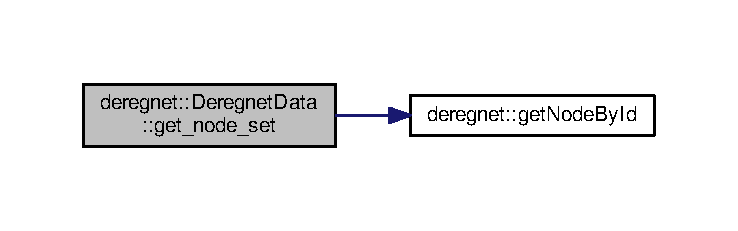
\includegraphics[width=350pt]{classderegnet_1_1DeregnetData_a7d662c0dd84d814bbaaf56718a99306a_cgraph}
\end{center}
\end{figure}
Here is the caller graph for this function\+:\nopagebreak
\begin{figure}[H]
\begin{center}
\leavevmode
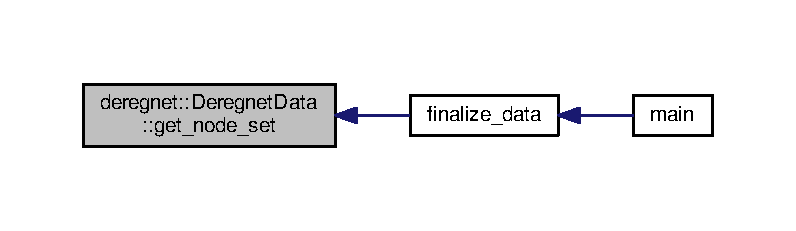
\includegraphics[width=350pt]{classderegnet_1_1DeregnetData_a7d662c0dd84d814bbaaf56718a99306a_icgraph}
\end{center}
\end{figure}
\mbox{\Hypertarget{classderegnet_1_1DeregnetData_aaef262d5ca460f10851b25c01ad2f9bc}\label{classderegnet_1_1DeregnetData_aaef262d5ca460f10851b25c01ad2f9bc}} 
\index{deregnet\+::\+Deregnet\+Data@{deregnet\+::\+Deregnet\+Data}!get\+\_\+root@{get\+\_\+root}}
\index{get\+\_\+root@{get\+\_\+root}!deregnet\+::\+Deregnet\+Data@{deregnet\+::\+Deregnet\+Data}}
\subsubsection{\texorpdfstring{get\+\_\+root()}{get\_root()}}
{\footnotesize\ttfamily void deregnet\+::\+Deregnet\+Data\+::get\+\_\+root (\begin{DoxyParamCaption}\item[{std\+::string $\ast$}]{root\+\_\+id }\end{DoxyParamCaption})}



Get (Lemon) node corresponding to the id of the root. 

Updates \hyperlink{classderegnet_1_1DeregnetData_a51a22fd88f929b1b1a00edb409b4cd55}{Deregnet\+Data.\+root}


\begin{DoxyParams}{Parameters}
{\em root\+\_\+id} & Node id of the root node (null if none specified) \\
\hline
\end{DoxyParams}


Definition at line 138 of file Deregnet\+Data.\+cpp.



References deregnet\+::get\+Node\+By\+Id(), and I\+N\+P\+U\+T\+\_\+\+E\+R\+R\+OR.



Referenced by finalize\+\_\+data().


\begin{DoxyCode}
138                                               \{
139     \textcolor{keywordflow}{if} (root\_id) \{
140         \hyperlink{classderegnet_1_1DeregnetData_a51a22fd88f929b1b1a00edb409b4cd55}{root} = \textcolor{keyword}{new} \hyperlink{namespacederegnet_a744bad34f2de9856d36715a445f027f3}{Node}();
141         \textcolor{keywordflow}{if} (!\hyperlink{namespacederegnet_afefc9088a0ea47e8d8c1225b5de29244}{getNodeById}(\hyperlink{classderegnet_1_1DeregnetData_ab76d30fa2ef87099faecb31e3f95b6d6}{graph}, \hyperlink{classderegnet_1_1DeregnetData_a3b57d7ed19c104c7fe257e17f0d2cfb5}{nodeid}, *root\_id, \hyperlink{classderegnet_1_1DeregnetData_a51a22fd88f929b1b1a00edb409b4cd55}{root})) \{
142             cerr << \textcolor{stringliteral}{"Root seems not to be in the graph."} << endl;
143             exit(\hyperlink{DeregnetData_8hpp_a288116f92845fddefeb044f5b84bc889}{INPUT\_ERROR});
144         \}
145     \}
146 \}
\end{DoxyCode}
Here is the call graph for this function\+:\nopagebreak
\begin{figure}[H]
\begin{center}
\leavevmode
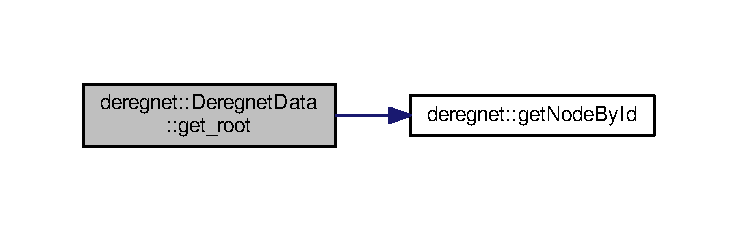
\includegraphics[width=350pt]{classderegnet_1_1DeregnetData_aaef262d5ca460f10851b25c01ad2f9bc_cgraph}
\end{center}
\end{figure}
Here is the caller graph for this function\+:\nopagebreak
\begin{figure}[H]
\begin{center}
\leavevmode
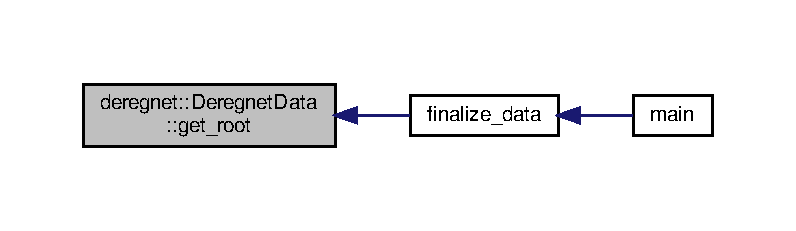
\includegraphics[width=350pt]{classderegnet_1_1DeregnetData_aaef262d5ca460f10851b25c01ad2f9bc_icgraph}
\end{center}
\end{figure}
\mbox{\Hypertarget{classderegnet_1_1DeregnetData_ae5edd8f077b20056f416d42ef3fb03d2}\label{classderegnet_1_1DeregnetData_ae5edd8f077b20056f416d42ef3fb03d2}} 
\index{deregnet\+::\+Deregnet\+Data@{deregnet\+::\+Deregnet\+Data}!read\+\_\+graph@{read\+\_\+graph}}
\index{read\+\_\+graph@{read\+\_\+graph}!deregnet\+::\+Deregnet\+Data@{deregnet\+::\+Deregnet\+Data}}
\subsubsection{\texorpdfstring{read\+\_\+graph()}{read\_graph()}}
{\footnotesize\ttfamily void deregnet\+::\+Deregnet\+Data\+::read\+\_\+graph (\begin{DoxyParamCaption}\item[{std\+::string $\ast$}]{path\+To\+Lgf }\end{DoxyParamCaption})}



Read graph from L\+GF (Lemon Graph Format) file. 

\href{http://lemon.cs.elte.hu/pub/tutorial/a00018.html}{\tt http\+://lemon.\+cs.\+elte.\+hu/pub/tutorial/a00018.\+html}


\begin{DoxyParams}{Parameters}
{\em path\+To\+Lgf} & Path to L\+GF file \\
\hline
\end{DoxyParams}


Definition at line 58 of file Deregnet\+Data.\+cpp.



References I\+N\+P\+U\+T\+\_\+\+E\+R\+R\+OR.



Referenced by finalize\+\_\+data().


\begin{DoxyCode}
58                                                \{
59     \textcolor{keywordflow}{if} (!pathToLgf) \{
60         cerr << \textcolor{stringliteral}{"No lgf specified."} << endl;
61         exit(\hyperlink{DeregnetData_8hpp_a288116f92845fddefeb044f5b84bc889}{INPUT\_ERROR});
62     \}
63     \hyperlink{classderegnet_1_1DeregnetData_ab76d30fa2ef87099faecb31e3f95b6d6}{graph} = \textcolor{keyword}{new} \hyperlink{namespacederegnet_a55b76c55bbabc682cbc61f8b9948799e}{Graph}();
64     \hyperlink{classderegnet_1_1DeregnetData_a3b57d7ed19c104c7fe257e17f0d2cfb5}{nodeid} = \textcolor{keyword}{new} NodeMap<string>(*graph);
65     \textcolor{keywordflow}{try} \{
66         digraphReader(*graph, *pathToLgf)
67         .nodeMap(\textcolor{stringliteral}{"id"}, *\hyperlink{classderegnet_1_1DeregnetData_a3b57d7ed19c104c7fe257e17f0d2cfb5}{nodeid})
68         .run();
69     \}
70     \textcolor{keywordflow}{catch} ( ... ) \{
71         cerr << \textcolor{stringliteral}{"Could not read lgf file "} << pathToLgf << \textcolor{stringliteral}{"."} << endl;
72         exit(\hyperlink{DeregnetData_8hpp_a288116f92845fddefeb044f5b84bc889}{INPUT\_ERROR});
73     \}
74     \textcolor{keywordflow}{if} (!\hyperlink{classderegnet_1_1DeregnetData_ae7936fe59661a68464134b9251303727}{receptor\_as\_root})
75         \hyperlink{classderegnet_1_1DeregnetData_aa36e9ddbc2d055ac7661e74f8fa76da4}{reverse\_graph}();
76     \textcolor{keywordflow}{else}
77         \hyperlink{classderegnet_1_1DeregnetData_a3ea2abe9900785d80fa0141afdd985a9}{original\_graph} = \hyperlink{classderegnet_1_1DeregnetData_ab76d30fa2ef87099faecb31e3f95b6d6}{graph};
78 \}
\end{DoxyCode}
Here is the caller graph for this function\+:\nopagebreak
\begin{figure}[H]
\begin{center}
\leavevmode
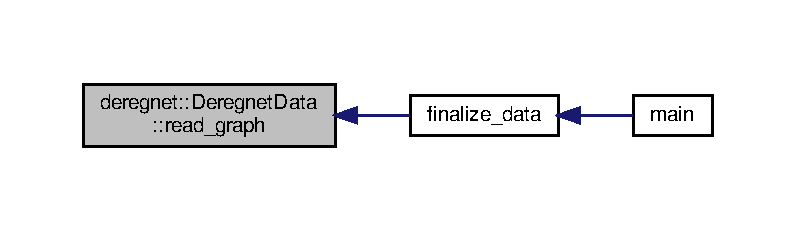
\includegraphics[width=350pt]{classderegnet_1_1DeregnetData_ae5edd8f077b20056f416d42ef3fb03d2_icgraph}
\end{center}
\end{figure}
\mbox{\Hypertarget{classderegnet_1_1DeregnetData_a01308048556370738e4ac335aba62ffd}\label{classderegnet_1_1DeregnetData_a01308048556370738e4ac335aba62ffd}} 
\index{deregnet\+::\+Deregnet\+Data@{deregnet\+::\+Deregnet\+Data}!read\+\_\+score@{read\+\_\+score}}
\index{read\+\_\+score@{read\+\_\+score}!deregnet\+::\+Deregnet\+Data@{deregnet\+::\+Deregnet\+Data}}
\subsubsection{\texorpdfstring{read\+\_\+score()}{read\_score()}}
{\footnotesize\ttfamily void deregnet\+::\+Deregnet\+Data\+::read\+\_\+score (\begin{DoxyParamCaption}\item[{std\+::string $\ast$}]{path\+To\+Tsv,  }\item[{bool}]{take\+\_\+abs }\end{DoxyParamCaption})}



Read scores from file. 


\begin{DoxyParams}{Parameters}
{\em path\+To\+Tsv} & Path to file with scores\+: two columns tab-\/seperated, first column\+: node id\textquotesingle{}s \\
\hline
{\em take\+\_\+abs} & Whether to take the absolute values of the parsed scores as actual score \\
\hline
\end{DoxyParams}


Definition at line 80 of file Deregnet\+Data.\+cpp.



References I\+N\+P\+U\+T\+\_\+\+E\+R\+R\+OR, and I\+N\+V\+A\+L\+ID.



Referenced by finalize\+\_\+data().


\begin{DoxyCode}
80                                                               \{
81     \textcolor{keywordflow}{if} (!\hyperlink{classderegnet_1_1DeregnetData_ab76d30fa2ef87099faecb31e3f95b6d6}{graph}) \{
82         cerr << \textcolor{stringliteral}{"Error: call AvgDeregnetData::read\_graph() first."} << endl;
83         exit(\hyperlink{DeregnetData_8hpp_a288116f92845fddefeb044f5b84bc889}{INPUT\_ERROR});
84     \}
85     \textcolor{keywordflow}{if} (!pathToTsv) \{
86         cerr << \textcolor{stringliteral}{"No score file specified."} << endl;
87         exit(\hyperlink{DeregnetData_8hpp_a288116f92845fddefeb044f5b84bc889}{INPUT\_ERROR});
88     \}
89     map<string, std::set<double>> score\_map;
90     \textcolor{keywordflow}{try} \{
91         ifstream tsv;
92         tsv.open( *pathToTsv );
93         \textcolor{keywordtype}{string} key;
94         \textcolor{keywordtype}{double} value;
95         \textcolor{keywordflow}{while} ( !tsv.eof() ) \{
96               tsv >> key >> value;
97               \textcolor{keywordflow}{if} (take\_abs)
98                   value = std::abs(value);
99               \textcolor{keywordflow}{if} (score\_map.find(key) != score\_map.end())
100                   score\_map[key].insert(value);
101               \textcolor{keywordflow}{else}
102                   score\_map[key] = \{ value \};        
103         \}
104         \hyperlink{classderegnet_1_1DeregnetData_a32970c8f43eb8be313ad08d829223b1f}{score} = \textcolor{keyword}{new} NodeMap<double>(*graph);
105         \textcolor{keywordflow}{for} (\hyperlink{namespacederegnet_ac34314e1b5f456fc6d1bb9d96316de4a}{NodeIt} v(*graph); v != \hyperlink{usinglemon_8hpp_adf770fe2eec438e3758ffe905dbae208}{INVALID}; ++v) \{
106             std::set<double> score\_set = score\_map[(*nodeid)[v]];
107             \textcolor{keywordflow}{if} (score\_set.size() == 0)
108                 (*\hyperlink{classderegnet_1_1DeregnetData_a32970c8f43eb8be313ad08d829223b1f}{score})[v] = 0.0;
109             \textcolor{keywordflow}{else}
110                 (*\hyperlink{classderegnet_1_1DeregnetData_a32970c8f43eb8be313ad08d829223b1f}{score})[v] = std::accumulate(score\_set.begin(), score\_set.end(), 0.0) / score\_set.
      size();
111                 
112 \textcolor{comment}{//            std::cout << (*nodeid)[v] << " : " << (*score)[v] << std::endl;}
113         \}
114         tsv.close();
115     \}
116     \textcolor{keywordflow}{catch} ( ... ) \{
117       cerr << \textcolor{stringliteral}{"Could not read score file "} << pathToTsv << \textcolor{stringliteral}{"."} << endl;
118       exit(\hyperlink{DeregnetData_8hpp_a288116f92845fddefeb044f5b84bc889}{INPUT\_ERROR});
119     \}
120 \}
\end{DoxyCode}
Here is the caller graph for this function\+:\nopagebreak
\begin{figure}[H]
\begin{center}
\leavevmode
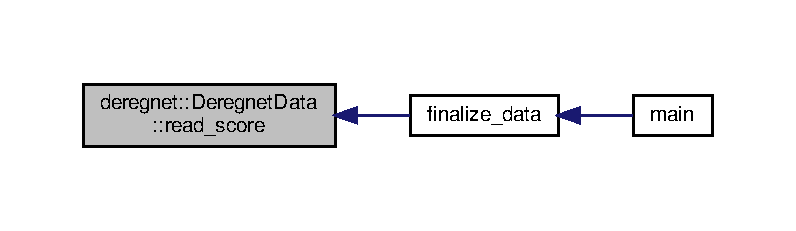
\includegraphics[width=350pt]{classderegnet_1_1DeregnetData_a01308048556370738e4ac335aba62ffd_icgraph}
\end{center}
\end{figure}
\mbox{\Hypertarget{classderegnet_1_1DeregnetData_aa36e9ddbc2d055ac7661e74f8fa76da4}\label{classderegnet_1_1DeregnetData_aa36e9ddbc2d055ac7661e74f8fa76da4}} 
\index{deregnet\+::\+Deregnet\+Data@{deregnet\+::\+Deregnet\+Data}!reverse\+\_\+graph@{reverse\+\_\+graph}}
\index{reverse\+\_\+graph@{reverse\+\_\+graph}!deregnet\+::\+Deregnet\+Data@{deregnet\+::\+Deregnet\+Data}}
\subsubsection{\texorpdfstring{reverse\+\_\+graph()}{reverse\_graph()}}
{\footnotesize\ttfamily void deregnet\+::\+Deregnet\+Data\+::reverse\+\_\+graph (\begin{DoxyParamCaption}{ }\end{DoxyParamCaption})\hspace{0.3cm}{\ttfamily [private]}}



Reverse orientation of edges in original input graph. 



Definition at line 148 of file Deregnet\+Data.\+cpp.



References I\+N\+V\+A\+L\+ID.


\begin{DoxyCode}
148                                  \{
149     map<Node,Node> node\_correspondence;
150     \hyperlink{classderegnet_1_1DeregnetData_a4b6a17e13aeda78317ff37567e7fd26d}{revgraph} = \textcolor{keyword}{new} \hyperlink{namespacederegnet_a55b76c55bbabc682cbc61f8b9948799e}{Graph}();
151     \hyperlink{classderegnet_1_1DeregnetData_ad15bd1f0e5ab9d01b82b5c696203b855}{revnodeid} = \textcolor{keyword}{new} NodeMap<string>(*revgraph);
152     \textcolor{keywordflow}{for} (\hyperlink{namespacederegnet_ac34314e1b5f456fc6d1bb9d96316de4a}{NodeIt} v(*\hyperlink{classderegnet_1_1DeregnetData_ab76d30fa2ef87099faecb31e3f95b6d6}{graph}); v != \hyperlink{usinglemon_8hpp_adf770fe2eec438e3758ffe905dbae208}{INVALID}; ++v) \{
153         \hyperlink{namespacederegnet_a744bad34f2de9856d36715a445f027f3}{Node} revv = revgraph->addNode();
154         (*revnodeid)[revv] = (*nodeid)[v];
155         node\_correspondence[v] = revv;
156     \}
157     \textcolor{keywordflow}{for} (\hyperlink{namespacederegnet_ac34314e1b5f456fc6d1bb9d96316de4a}{NodeIt} v(*\hyperlink{classderegnet_1_1DeregnetData_ab76d30fa2ef87099faecb31e3f95b6d6}{graph}); v != \hyperlink{usinglemon_8hpp_adf770fe2eec438e3758ffe905dbae208}{INVALID}; ++v) \{
158         \hyperlink{namespacederegnet_a744bad34f2de9856d36715a445f027f3}{Node} revv = node\_correspondence[v];
159         \textcolor{keywordflow}{for} (\hyperlink{namespacederegnet_aed58be361aeda4ef7a9eaca2731ba830}{InArcIt} a(*\hyperlink{classderegnet_1_1DeregnetData_ab76d30fa2ef87099faecb31e3f95b6d6}{graph}, v); a != \hyperlink{usinglemon_8hpp_adf770fe2eec438e3758ffe905dbae208}{INVALID}; ++a) \{
160             \hyperlink{namespacederegnet_a744bad34f2de9856d36715a445f027f3}{Node} s = \hyperlink{classderegnet_1_1DeregnetData_ab76d30fa2ef87099faecb31e3f95b6d6}{graph}->source(a);
161             \hyperlink{namespacederegnet_a744bad34f2de9856d36715a445f027f3}{Node} revs = node\_correspondence[s];
162             revgraph->addArc(revv,revs);
163         \}
164     \}
165     \hyperlink{classderegnet_1_1DeregnetData_a3ea2abe9900785d80fa0141afdd985a9}{original\_graph} = \hyperlink{classderegnet_1_1DeregnetData_ab76d30fa2ef87099faecb31e3f95b6d6}{graph};
166     \hyperlink{classderegnet_1_1DeregnetData_a6707f9bbc1ac5ccf78724e73cd8053b1}{original\_nodeid} = \hyperlink{classderegnet_1_1DeregnetData_a3b57d7ed19c104c7fe257e17f0d2cfb5}{nodeid};
167     \hyperlink{classderegnet_1_1DeregnetData_ab76d30fa2ef87099faecb31e3f95b6d6}{graph} = \hyperlink{classderegnet_1_1DeregnetData_a4b6a17e13aeda78317ff37567e7fd26d}{revgraph};
168     \hyperlink{classderegnet_1_1DeregnetData_a3b57d7ed19c104c7fe257e17f0d2cfb5}{nodeid} = \hyperlink{classderegnet_1_1DeregnetData_ad15bd1f0e5ab9d01b82b5c696203b855}{revnodeid};
169     swap(\hyperlink{classderegnet_1_1DeregnetData_a470cc9f84741c59897ab1e7a3daa1205}{receptors}, \hyperlink{classderegnet_1_1DeregnetData_a1fe559c6056cd411647f836849e4b0da}{terminals});
170 \}
\end{DoxyCode}


\subsection{Member Data Documentation}
\mbox{\Hypertarget{classderegnet_1_1DeregnetData_a8e4398e6ece11ef87767914c6f2c304d}\label{classderegnet_1_1DeregnetData_a8e4398e6ece11ef87767914c6f2c304d}} 
\index{deregnet\+::\+Deregnet\+Data@{deregnet\+::\+Deregnet\+Data}!exclude@{exclude}}
\index{exclude@{exclude}!deregnet\+::\+Deregnet\+Data@{deregnet\+::\+Deregnet\+Data}}
\subsubsection{\texorpdfstring{exclude}{exclude}}
{\footnotesize\ttfamily std\+::set$<$\hyperlink{namespacederegnet_a744bad34f2de9856d36715a445f027f3}{Node}$>$$\ast$ deregnet\+::\+Deregnet\+Data\+::exclude \{ nullptr \}}



Nodes excluded from any subgraph a priori. 



Definition at line 67 of file Deregnet\+Data.\+hpp.



Referenced by finalize\+\_\+data(), deregnet\+::\+Deregnet\+Finder$<$ Model\+Type, Data $>$\+::find\+\_\+start\+\_\+solution(), deregnet\+::\+Deregnet\+Finder$<$ Model\+Type, Data $>$\+::find\+\_\+suboptimal\+\_\+start\+\_\+solution(), and deregnet\+::\+Deregnet\+Finder$<$ Model\+Type, Data $>$\+::run\+\_\+optimal\+\_\+init().

\mbox{\Hypertarget{classderegnet_1_1DeregnetData_a3637c87366454adc152487fc2f5cfede}\label{classderegnet_1_1DeregnetData_a3637c87366454adc152487fc2f5cfede}} 
\index{deregnet\+::\+Deregnet\+Data@{deregnet\+::\+Deregnet\+Data}!gap\+\_\+cut@{gap\+\_\+cut}}
\index{gap\+\_\+cut@{gap\+\_\+cut}!deregnet\+::\+Deregnet\+Data@{deregnet\+::\+Deregnet\+Data}}
\subsubsection{\texorpdfstring{gap\+\_\+cut}{gap\_cut}}
{\footnotesize\ttfamily double$\ast$ deregnet\+::\+Deregnet\+Data\+::gap\+\_\+cut \{ nullptr \}}



Gap tolerance. 



Definition at line 71 of file Deregnet\+Data.\+hpp.



Referenced by finalize\+\_\+data(), and parse\+\_\+options().

\mbox{\Hypertarget{classderegnet_1_1DeregnetData_ab76d30fa2ef87099faecb31e3f95b6d6}\label{classderegnet_1_1DeregnetData_ab76d30fa2ef87099faecb31e3f95b6d6}} 
\index{deregnet\+::\+Deregnet\+Data@{deregnet\+::\+Deregnet\+Data}!graph@{graph}}
\index{graph@{graph}!deregnet\+::\+Deregnet\+Data@{deregnet\+::\+Deregnet\+Data}}
\subsubsection{\texorpdfstring{graph}{graph}}
{\footnotesize\ttfamily \hyperlink{namespacederegnet_a55b76c55bbabc682cbc61f8b9948799e}{Graph}$\ast$ deregnet\+::\+Deregnet\+Data\+::graph \{ nullptr \}}



Actual graph used to run the algorithms. 



Definition at line 59 of file Deregnet\+Data.\+hpp.



Referenced by deregnet\+::\+Deregnet\+Model$<$ Model\+Type, deregnet\+::\+Avgdrgnt\+Data $>$\+::\+Deregnet\+Model(), finalize\+\_\+data(), deregnet\+::\+Deregnet\+Finder$<$ Model\+Type, Data $>$\+::find\+\_\+start\+\_\+solution(), and deregnet\+::\+Deregnet\+Finder$<$ Model\+Type, Data $>$\+::find\+\_\+suboptimal\+\_\+start\+\_\+solution().

\mbox{\Hypertarget{classderegnet_1_1DeregnetData_a438d16e60be5d119d174aa039f070ab2}\label{classderegnet_1_1DeregnetData_a438d16e60be5d119d174aa039f070ab2}} 
\index{deregnet\+::\+Deregnet\+Data@{deregnet\+::\+Deregnet\+Data}!include@{include}}
\index{include@{include}!deregnet\+::\+Deregnet\+Data@{deregnet\+::\+Deregnet\+Data}}
\subsubsection{\texorpdfstring{include}{include}}
{\footnotesize\ttfamily std\+::set$<$\hyperlink{namespacederegnet_a744bad34f2de9856d36715a445f027f3}{Node}$>$$\ast$ deregnet\+::\+Deregnet\+Data\+::include \{ nullptr \}}



Nodes included in any subgraph a priori. 



Definition at line 66 of file Deregnet\+Data.\+hpp.



Referenced by finalize\+\_\+data(), and deregnet\+::\+Deregnet\+Finder$<$ Model\+Type, Data $>$\+::run\+\_\+optimal\+\_\+init().

\mbox{\Hypertarget{classderegnet_1_1DeregnetData_a43111d8664fd9db36f36f75b24ba62e9}\label{classderegnet_1_1DeregnetData_a43111d8664fd9db36f36f75b24ba62e9}} 
\index{deregnet\+::\+Deregnet\+Data@{deregnet\+::\+Deregnet\+Data}!max\+\_\+overlap@{max\+\_\+overlap}}
\index{max\+\_\+overlap@{max\+\_\+overlap}!deregnet\+::\+Deregnet\+Data@{deregnet\+::\+Deregnet\+Data}}
\subsubsection{\texorpdfstring{max\+\_\+overlap}{max\_overlap}}
{\footnotesize\ttfamily double deregnet\+::\+Deregnet\+Data\+::max\+\_\+overlap \{ 0.\+0 \}}



Maximal percentage of overlap to previous subgraphs when searching for suboptimal subgraphs. 



Definition at line 69 of file Deregnet\+Data.\+hpp.



Referenced by deregnet\+::\+Deregnet\+Finder$<$ Model\+Type, Data $>$\+::find\+\_\+suboptimal\+\_\+start\+\_\+solution(), and parse\+\_\+options().

\mbox{\Hypertarget{classderegnet_1_1DeregnetData_ac3918536b5423facf0ac155997703c52}\label{classderegnet_1_1DeregnetData_ac3918536b5423facf0ac155997703c52}} 
\index{deregnet\+::\+Deregnet\+Data@{deregnet\+::\+Deregnet\+Data}!model\+\_\+sense@{model\+\_\+sense}}
\index{model\+\_\+sense@{model\+\_\+sense}!deregnet\+::\+Deregnet\+Data@{deregnet\+::\+Deregnet\+Data}}
\subsubsection{\texorpdfstring{model\+\_\+sense}{model\_sense}}
{\footnotesize\ttfamily std\+::string deregnet\+::\+Deregnet\+Data\+::model\+\_\+sense \{ \char`\"{}max\char`\"{} \}}



Whether to maximize or minimize. 



Definition at line 73 of file Deregnet\+Data.\+hpp.



Referenced by deregnet\+::\+Deregnet\+Finder$<$ Model\+Type, Data $>$\+::find\+\_\+start\+\_\+solution(), deregnet\+::\+Deregnet\+Finder$<$ Model\+Type, Data $>$\+::find\+\_\+suboptimal\+\_\+start\+\_\+solution(), and parse\+\_\+options().

\mbox{\Hypertarget{classderegnet_1_1DeregnetData_a3b57d7ed19c104c7fe257e17f0d2cfb5}\label{classderegnet_1_1DeregnetData_a3b57d7ed19c104c7fe257e17f0d2cfb5}} 
\index{deregnet\+::\+Deregnet\+Data@{deregnet\+::\+Deregnet\+Data}!nodeid@{nodeid}}
\index{nodeid@{nodeid}!deregnet\+::\+Deregnet\+Data@{deregnet\+::\+Deregnet\+Data}}
\subsubsection{\texorpdfstring{nodeid}{nodeid}}
{\footnotesize\ttfamily \hyperlink{namespacederegnet_ae102b707ae1d6f83c639ece5e0dd5658}{Node\+Map}$<$std\+::string$>$$\ast$ deregnet\+::\+Deregnet\+Data\+::nodeid \{ nullptr \}}



Node id\textquotesingle{}s. 



Definition at line 62 of file Deregnet\+Data.\+hpp.



Referenced by deregnet\+::\+Deregnet\+Finder$<$ Model\+Type, Data $>$\+::find\+\_\+suboptimal\+\_\+start\+\_\+solution(), and deregnet\+::\+Deregnet\+Finder$<$ Model\+Type, Data $>$\+::to\+\_\+subgraph().

\mbox{\Hypertarget{classderegnet_1_1DeregnetData_adb7428cd99112156ae9f80187af9ebbe}\label{classderegnet_1_1DeregnetData_adb7428cd99112156ae9f80187af9ebbe}} 
\index{deregnet\+::\+Deregnet\+Data@{deregnet\+::\+Deregnet\+Data}!num\+\_\+subopt\+\_\+iter@{num\+\_\+subopt\+\_\+iter}}
\index{num\+\_\+subopt\+\_\+iter@{num\+\_\+subopt\+\_\+iter}!deregnet\+::\+Deregnet\+Data@{deregnet\+::\+Deregnet\+Data}}
\subsubsection{\texorpdfstring{num\+\_\+subopt\+\_\+iter}{num\_subopt\_iter}}
{\footnotesize\ttfamily int deregnet\+::\+Deregnet\+Data\+::num\+\_\+subopt\+\_\+iter \{ 0 \}}



Number of iterations to find suboptimal subgraphs. 



Definition at line 68 of file Deregnet\+Data.\+hpp.



Referenced by parse\+\_\+options(), and deregnet\+::\+Deregnet\+Finder$<$ Model\+Type, Data $>$\+::run().

\mbox{\Hypertarget{classderegnet_1_1DeregnetData_a3ea2abe9900785d80fa0141afdd985a9}\label{classderegnet_1_1DeregnetData_a3ea2abe9900785d80fa0141afdd985a9}} 
\index{deregnet\+::\+Deregnet\+Data@{deregnet\+::\+Deregnet\+Data}!original\+\_\+graph@{original\+\_\+graph}}
\index{original\+\_\+graph@{original\+\_\+graph}!deregnet\+::\+Deregnet\+Data@{deregnet\+::\+Deregnet\+Data}}
\subsubsection{\texorpdfstring{original\+\_\+graph}{original\_graph}}
{\footnotesize\ttfamily \hyperlink{namespacederegnet_a55b76c55bbabc682cbc61f8b9948799e}{Graph}$\ast$ deregnet\+::\+Deregnet\+Data\+::original\+\_\+graph \{ nullptr \}}



Original input graph. 



Definition at line 60 of file Deregnet\+Data.\+hpp.



Referenced by deregnet\+::\+Deregnet\+Finder$<$ Model\+Type, Data $>$\+::to\+\_\+subgraph().

\mbox{\Hypertarget{classderegnet_1_1DeregnetData_a6707f9bbc1ac5ccf78724e73cd8053b1}\label{classderegnet_1_1DeregnetData_a6707f9bbc1ac5ccf78724e73cd8053b1}} 
\index{deregnet\+::\+Deregnet\+Data@{deregnet\+::\+Deregnet\+Data}!original\+\_\+nodeid@{original\+\_\+nodeid}}
\index{original\+\_\+nodeid@{original\+\_\+nodeid}!deregnet\+::\+Deregnet\+Data@{deregnet\+::\+Deregnet\+Data}}
\subsubsection{\texorpdfstring{original\+\_\+nodeid}{original\_nodeid}}
{\footnotesize\ttfamily \hyperlink{namespacederegnet_ae102b707ae1d6f83c639ece5e0dd5658}{Node\+Map}$<$std\+::string$>$$\ast$ deregnet\+::\+Deregnet\+Data\+::original\+\_\+nodeid \{ nullptr \}\hspace{0.3cm}{\ttfamily [private]}}



Definition at line 81 of file Deregnet\+Data.\+hpp.

\mbox{\Hypertarget{classderegnet_1_1DeregnetData_ae7936fe59661a68464134b9251303727}\label{classderegnet_1_1DeregnetData_ae7936fe59661a68464134b9251303727}} 
\index{deregnet\+::\+Deregnet\+Data@{deregnet\+::\+Deregnet\+Data}!receptor\+\_\+as\+\_\+root@{receptor\+\_\+as\+\_\+root}}
\index{receptor\+\_\+as\+\_\+root@{receptor\+\_\+as\+\_\+root}!deregnet\+::\+Deregnet\+Data@{deregnet\+::\+Deregnet\+Data}}
\subsubsection{\texorpdfstring{receptor\+\_\+as\+\_\+root}{receptor\_as\_root}}
{\footnotesize\ttfamily bool deregnet\+::\+Deregnet\+Data\+::receptor\+\_\+as\+\_\+root \{ true \}}



Whether to orient the subgraphs such that the root acts as \textquotesingle{}receptor\textquotesingle{}. 



Definition at line 72 of file Deregnet\+Data.\+hpp.



Referenced by parse\+\_\+options(), and deregnet\+::\+Deregnet\+Finder$<$ Model\+Type, Data $>$\+::to\+\_\+subgraph().

\mbox{\Hypertarget{classderegnet_1_1DeregnetData_a470cc9f84741c59897ab1e7a3daa1205}\label{classderegnet_1_1DeregnetData_a470cc9f84741c59897ab1e7a3daa1205}} 
\index{deregnet\+::\+Deregnet\+Data@{deregnet\+::\+Deregnet\+Data}!receptors@{receptors}}
\index{receptors@{receptors}!deregnet\+::\+Deregnet\+Data@{deregnet\+::\+Deregnet\+Data}}
\subsubsection{\texorpdfstring{receptors}{receptors}}
{\footnotesize\ttfamily std\+::set$<$\hyperlink{namespacederegnet_a744bad34f2de9856d36715a445f027f3}{Node}$>$$\ast$ deregnet\+::\+Deregnet\+Data\+::receptors \{ nullptr \}}



Nodes classified as \textquotesingle{}receptors\textquotesingle{}. 



Definition at line 65 of file Deregnet\+Data.\+hpp.



Referenced by finalize\+\_\+data(), deregnet\+::\+Deregnet\+Finder$<$ Model\+Type, Data $>$\+::find\+\_\+start\+\_\+solution(), deregnet\+::\+Deregnet\+Finder$<$ Model\+Type, Data $>$\+::find\+\_\+suboptimal\+\_\+start\+\_\+solution(), deregnet\+::\+Deregnet\+Finder$<$ Model\+Type, Data $>$\+::run\+\_\+optimal\+\_\+init(), and deregnet\+::\+Deregnet\+Finder$<$ Model\+Type, Data $>$\+::to\+\_\+subgraph().

\mbox{\Hypertarget{classderegnet_1_1DeregnetData_a4b6a17e13aeda78317ff37567e7fd26d}\label{classderegnet_1_1DeregnetData_a4b6a17e13aeda78317ff37567e7fd26d}} 
\index{deregnet\+::\+Deregnet\+Data@{deregnet\+::\+Deregnet\+Data}!revgraph@{revgraph}}
\index{revgraph@{revgraph}!deregnet\+::\+Deregnet\+Data@{deregnet\+::\+Deregnet\+Data}}
\subsubsection{\texorpdfstring{revgraph}{revgraph}}
{\footnotesize\ttfamily \hyperlink{namespacederegnet_a55b76c55bbabc682cbc61f8b9948799e}{Graph}$\ast$ deregnet\+::\+Deregnet\+Data\+::revgraph \{ nullptr \}\hspace{0.3cm}{\ttfamily [private]}}



Definition at line 79 of file Deregnet\+Data.\+hpp.

\mbox{\Hypertarget{classderegnet_1_1DeregnetData_ad15bd1f0e5ab9d01b82b5c696203b855}\label{classderegnet_1_1DeregnetData_ad15bd1f0e5ab9d01b82b5c696203b855}} 
\index{deregnet\+::\+Deregnet\+Data@{deregnet\+::\+Deregnet\+Data}!revnodeid@{revnodeid}}
\index{revnodeid@{revnodeid}!deregnet\+::\+Deregnet\+Data@{deregnet\+::\+Deregnet\+Data}}
\subsubsection{\texorpdfstring{revnodeid}{revnodeid}}
{\footnotesize\ttfamily \hyperlink{namespacederegnet_ae102b707ae1d6f83c639ece5e0dd5658}{Node\+Map}$<$std\+::string$>$$\ast$ deregnet\+::\+Deregnet\+Data\+::revnodeid \{ nullptr \}\hspace{0.3cm}{\ttfamily [private]}}



Definition at line 78 of file Deregnet\+Data.\+hpp.

\mbox{\Hypertarget{classderegnet_1_1DeregnetData_a51a22fd88f929b1b1a00edb409b4cd55}\label{classderegnet_1_1DeregnetData_a51a22fd88f929b1b1a00edb409b4cd55}} 
\index{deregnet\+::\+Deregnet\+Data@{deregnet\+::\+Deregnet\+Data}!root@{root}}
\index{root@{root}!deregnet\+::\+Deregnet\+Data@{deregnet\+::\+Deregnet\+Data}}
\subsubsection{\texorpdfstring{root}{root}}
{\footnotesize\ttfamily \hyperlink{namespacederegnet_a744bad34f2de9856d36715a445f027f3}{Node}$\ast$ deregnet\+::\+Deregnet\+Data\+::root \{ nullptr \}}



Root node (null if the algorithm is supposed to find the root) 



Definition at line 63 of file Deregnet\+Data.\+hpp.



Referenced by deregnet\+::\+Deregnet\+Finder$<$ Model\+Type, Data $>$\+::find\+\_\+start\+\_\+solution(), deregnet\+::\+Deregnet\+Finder$<$ Model\+Type, Data $>$\+::find\+\_\+suboptimal\+\_\+start\+\_\+solution(), and deregnet\+::\+Deregnet\+Finder$<$ Model\+Type, Data $>$\+::run\+\_\+optimal\+\_\+init().

\mbox{\Hypertarget{classderegnet_1_1DeregnetData_a32970c8f43eb8be313ad08d829223b1f}\label{classderegnet_1_1DeregnetData_a32970c8f43eb8be313ad08d829223b1f}} 
\index{deregnet\+::\+Deregnet\+Data@{deregnet\+::\+Deregnet\+Data}!score@{score}}
\index{score@{score}!deregnet\+::\+Deregnet\+Data@{deregnet\+::\+Deregnet\+Data}}
\subsubsection{\texorpdfstring{score}{score}}
{\footnotesize\ttfamily \hyperlink{namespacederegnet_ae102b707ae1d6f83c639ece5e0dd5658}{Node\+Map}$<$double$>$$\ast$ deregnet\+::\+Deregnet\+Data\+::score \{ nullptr \}}



Node scores. 



Definition at line 61 of file Deregnet\+Data.\+hpp.



Referenced by deregnet\+::\+Deregnet\+Finder$<$ Model\+Type, Data $>$\+::find\+\_\+start\+\_\+solution(), and deregnet\+::\+Deregnet\+Finder$<$ Model\+Type, Data $>$\+::find\+\_\+suboptimal\+\_\+start\+\_\+solution().

\mbox{\Hypertarget{classderegnet_1_1DeregnetData_abac721360704af5615f7ff84b183eebd}\label{classderegnet_1_1DeregnetData_abac721360704af5615f7ff84b183eebd}} 
\index{deregnet\+::\+Deregnet\+Data@{deregnet\+::\+Deregnet\+Data}!start\+\_\+heuristic@{start\+\_\+heuristic}}
\index{start\+\_\+heuristic@{start\+\_\+heuristic}!deregnet\+::\+Deregnet\+Data@{deregnet\+::\+Deregnet\+Data}}
\subsubsection{\texorpdfstring{start\+\_\+heuristic}{start\_heuristic}}
{\footnotesize\ttfamily bool deregnet\+::\+Deregnet\+Data\+::start\+\_\+heuristic \{ true \}}



Whether to run the greedy start heuristic. 



Definition at line 74 of file Deregnet\+Data.\+hpp.



Referenced by parse\+\_\+options(), deregnet\+::\+Deregnet\+Finder$<$ Model\+Type, Data $>$\+::run\+\_\+optimal\+\_\+init(), and deregnet\+::\+Deregnet\+Finder$<$ Model\+Type, Data $>$\+::run\+\_\+suboptimal\+\_\+init().

\mbox{\Hypertarget{classderegnet_1_1DeregnetData_a1fe559c6056cd411647f836849e4b0da}\label{classderegnet_1_1DeregnetData_a1fe559c6056cd411647f836849e4b0da}} 
\index{deregnet\+::\+Deregnet\+Data@{deregnet\+::\+Deregnet\+Data}!terminals@{terminals}}
\index{terminals@{terminals}!deregnet\+::\+Deregnet\+Data@{deregnet\+::\+Deregnet\+Data}}
\subsubsection{\texorpdfstring{terminals}{terminals}}
{\footnotesize\ttfamily std\+::set$<$\hyperlink{namespacederegnet_a744bad34f2de9856d36715a445f027f3}{Node}$>$$\ast$ deregnet\+::\+Deregnet\+Data\+::terminals \{ nullptr \}}



Nodes classified as \textquotesingle{}terminals\textquotesingle{}. 



Definition at line 64 of file Deregnet\+Data.\+hpp.



Referenced by finalize\+\_\+data(), deregnet\+::\+Deregnet\+Finder$<$ Model\+Type, Data $>$\+::run\+\_\+optimal\+\_\+init(), and deregnet\+::\+Deregnet\+Finder$<$ Model\+Type, Data $>$\+::to\+\_\+subgraph().

\mbox{\Hypertarget{classderegnet_1_1DeregnetData_ac378faf7e8466135b8dc0ced907d98ae}\label{classderegnet_1_1DeregnetData_ac378faf7e8466135b8dc0ced907d98ae}} 
\index{deregnet\+::\+Deregnet\+Data@{deregnet\+::\+Deregnet\+Data}!time\+\_\+limit@{time\+\_\+limit}}
\index{time\+\_\+limit@{time\+\_\+limit}!deregnet\+::\+Deregnet\+Data@{deregnet\+::\+Deregnet\+Data}}
\subsubsection{\texorpdfstring{time\+\_\+limit}{time\_limit}}
{\footnotesize\ttfamily double$\ast$ deregnet\+::\+Deregnet\+Data\+::time\+\_\+limit \{ nullptr \}}



Time limit of a single solve. 



Definition at line 70 of file Deregnet\+Data.\+hpp.



Referenced by parse\+\_\+options().



The documentation for this class was generated from the following files\+:\begin{DoxyCompactItemize}
\item 
/datadisk/bbubu/home/self/bbubu/projects/deregnet/src/\hyperlink{DeregnetData_8hpp}{Deregnet\+Data.\+hpp}\item 
/datadisk/bbubu/home/self/bbubu/projects/deregnet/src/\hyperlink{DeregnetData_8cpp}{Deregnet\+Data.\+cpp}\end{DoxyCompactItemize}

\hypertarget{classderegnet_1_1DeregnetFinder}{}\section{deregnet\+:\+:Deregnet\+Finder$<$ Model\+Type, Data $>$ Class Template Reference}
\label{classderegnet_1_1DeregnetFinder}\index{deregnet\+::\+Deregnet\+Finder$<$ Model\+Type, Data $>$@{deregnet\+::\+Deregnet\+Finder$<$ Model\+Type, Data $>$}}


Main entry point for running De\+Reg\+Net algorithms.  




{\ttfamily \#include $<$Deregnet\+Finder.\+hpp$>$}



Collaboration diagram for deregnet\+:\+:Deregnet\+Finder$<$ Model\+Type, Data $>$\+:\nopagebreak
\begin{figure}[H]
\begin{center}
\leavevmode
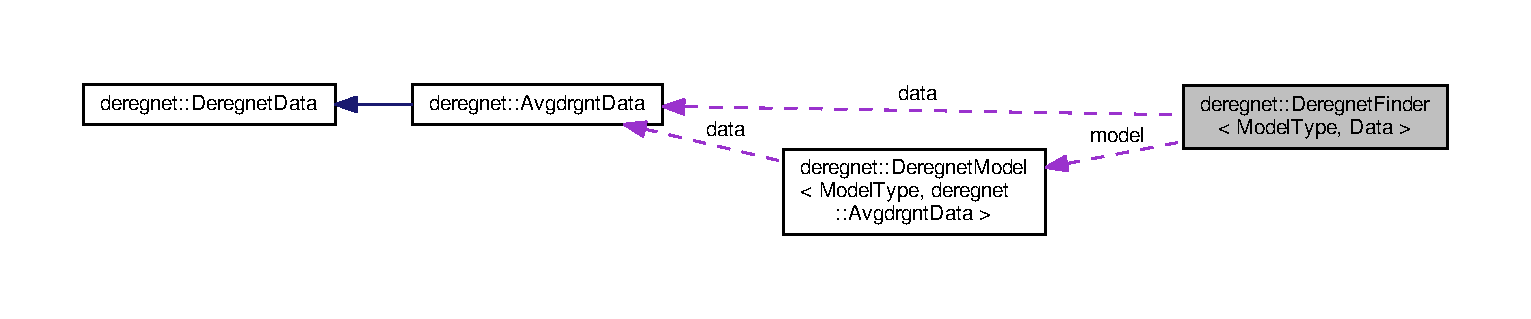
\includegraphics[width=350pt]{classderegnet_1_1DeregnetFinder__coll__graph}
\end{center}
\end{figure}
\subsection*{Public Member Functions}
\begin{DoxyCompactItemize}
\item 
\hyperlink{classderegnet_1_1DeregnetFinder_a5a19a86a0f9f9fa17e8ab625c748d31a}{Deregnet\+Finder} (\hyperlink{avgdrgnt_8cpp_a1d1235306db276e9b36acba1db1509e8}{Data} $\ast$xdata)
\begin{DoxyCompactList}\small\item\em Constructor, taking the relevant data as argument. \end{DoxyCompactList}\item 
std\+::vector$<$ \hyperlink{structderegnet_1_1Subgraph}{Subgraph} $>$ \hyperlink{classderegnet_1_1DeregnetFinder_a1a6119b306b54ff44d8c78f34fc037ab}{run} ()
\begin{DoxyCompactList}\small\item\em Method which finds the subgraphs. \end{DoxyCompactList}\item 
void \hyperlink{classderegnet_1_1DeregnetFinder_a9bca73c631c1ce679b07f1e0664abfa2}{find\+\_\+start\+\_\+solution} (std\+::pair$<$ \hyperlink{namespacederegnet_a744bad34f2de9856d36715a445f027f3}{Node}, std\+::set$<$ \hyperlink{namespacederegnet_a744bad34f2de9856d36715a445f027f3}{Node} $>$$>$ $\ast$$\ast$start\+\_\+solution)
\begin{DoxyCompactList}\small\item\em Finds a heuristic optimal start solution. \end{DoxyCompactList}\item 
void \hyperlink{classderegnet_1_1DeregnetFinder_a85fcde1dddbfd03ffc4ae8d244b4fc72}{find\+\_\+suboptimal\+\_\+start\+\_\+solution} (std\+::pair$<$ \hyperlink{namespacederegnet_a744bad34f2de9856d36715a445f027f3}{Node}, std\+::set$<$ \hyperlink{namespacederegnet_a744bad34f2de9856d36715a445f027f3}{Node} $>$$>$ $\ast$$\ast$start\+\_\+solution, std\+::set$<$ std\+::string $>$ $\ast$nodes\+\_\+so\+\_\+far)
\begin{DoxyCompactList}\small\item\em Finds a heuristic suboptimal start solution. \end{DoxyCompactList}\item 
\hyperlink{structderegnet_1_1Subgraph}{Subgraph} \hyperlink{classderegnet_1_1DeregnetFinder_a681d5e2506f9b6075ab36e742a360328}{to\+\_\+subgraph} (\hyperlink{structderegnet_1_1Solution}{Solution} solution, std\+::string signature)
\begin{DoxyCompactList}\small\item\em Transform a solution from the \hyperlink{structderegnet_1_1Solution}{Solution} type to the \hyperlink{structderegnet_1_1Subgraph}{Subgraph} type. \end{DoxyCompactList}\item 
{\footnotesize template$<$$>$ }\\void \hyperlink{classderegnet_1_1DeregnetFinder_a1b7a50c77d09000e2d80b39025d67393}{find\+\_\+start\+\_\+solution} (std\+::pair$<$ \hyperlink{namespacederegnet_a744bad34f2de9856d36715a445f027f3}{Node}, std\+::set$<$ \hyperlink{namespacederegnet_a744bad34f2de9856d36715a445f027f3}{Node} $>$$>$ $\ast$$\ast$start\+\_\+solution)
\item 
{\footnotesize template$<$$>$ }\\void \hyperlink{classderegnet_1_1DeregnetFinder_a6a5305626ad5039e294fa2f6bd3b4b74}{find\+\_\+start\+\_\+solution} (std\+::pair$<$ \hyperlink{namespacederegnet_a744bad34f2de9856d36715a445f027f3}{Node}, std\+::set$<$ \hyperlink{namespacederegnet_a744bad34f2de9856d36715a445f027f3}{Node} $>$$>$ $\ast$$\ast$start\+\_\+solution)
\item 
{\footnotesize template$<$$>$ }\\void \hyperlink{classderegnet_1_1DeregnetFinder_a42eca7055ed54197e27df7bd70271a13}{find\+\_\+suboptimal\+\_\+start\+\_\+solution} (std\+::pair$<$ \hyperlink{namespacederegnet_a744bad34f2de9856d36715a445f027f3}{Node}, std\+::set$<$ \hyperlink{namespacederegnet_a744bad34f2de9856d36715a445f027f3}{Node} $>$$>$ $\ast$$\ast$start\+\_\+solution, std\+::set$<$ std\+::string $>$ $\ast$nodes\+\_\+so\+\_\+far)
\item 
{\footnotesize template$<$$>$ }\\void \hyperlink{classderegnet_1_1DeregnetFinder_ae81ebb01d3cba09b12858bce7799e2a5}{find\+\_\+suboptimal\+\_\+start\+\_\+solution} (std\+::pair$<$ \hyperlink{namespacederegnet_a744bad34f2de9856d36715a445f027f3}{Node}, std\+::set$<$ \hyperlink{namespacederegnet_a744bad34f2de9856d36715a445f027f3}{Node} $>$$>$ $\ast$$\ast$start\+\_\+solution, std\+::set$<$ std\+::string $>$ $\ast$nodes\+\_\+so\+\_\+far)
\end{DoxyCompactItemize}
\subsection*{Private Member Functions}
\begin{DoxyCompactItemize}
\item 
void \hyperlink{classderegnet_1_1DeregnetFinder_ae0335349d6a60ee204d10bf8b7366cfa}{run\+\_\+optimal\+\_\+init} (std\+::pair$<$ \hyperlink{namespacederegnet_a744bad34f2de9856d36715a445f027f3}{Node}, std\+::set$<$ \hyperlink{namespacederegnet_a744bad34f2de9856d36715a445f027f3}{Node} $>$$>$ $\ast$$\ast$start\+\_\+solution)
\begin{DoxyCompactList}\small\item\em Preparation for finding the optimal subgraph. \end{DoxyCompactList}\item 
void \hyperlink{classderegnet_1_1DeregnetFinder_ad996cee997a5db4e09016a6f725a6701}{run\+\_\+suboptimal\+\_\+init} (std\+::pair$<$ \hyperlink{namespacederegnet_a744bad34f2de9856d36715a445f027f3}{Node}, std\+::set$<$ \hyperlink{namespacederegnet_a744bad34f2de9856d36715a445f027f3}{Node} $>$ $>$ $\ast$$\ast$start\+\_\+solution, std\+::set$<$ std\+::string $>$ $\ast$nodes\+\_\+so\+\_\+far)
\begin{DoxyCompactList}\small\item\em Perparation for finding suboptimal subgraphs. \end{DoxyCompactList}\item 
void \hyperlink{classderegnet_1_1DeregnetFinder_a92610c1444ba271820e64d224ec64bb7}{run\+\_\+optimal\+\_\+windup} (bool solve\+\_\+successful, std\+::vector$<$ \hyperlink{structderegnet_1_1Subgraph}{Subgraph} $>$ $\ast$subgraphs)
\begin{DoxyCompactList}\small\item\em Post-\/processing after attempt to find optimal subgraph. \end{DoxyCompactList}\item 
bool \hyperlink{classderegnet_1_1DeregnetFinder_a4021d92d787877187a24dcbaf0c1bad1}{run\+\_\+suboptimal\+\_\+windup} (bool solve\+\_\+successful, std\+::vector$<$ \hyperlink{structderegnet_1_1Subgraph}{Subgraph} $>$ $\ast$subgraphs, std\+::set$<$ std\+::string $>$ $\ast$nodes\+\_\+so\+\_\+far, int i)
\begin{DoxyCompactList}\small\item\em Post-\/processing after attempt to find suboptimal subgraphs. \end{DoxyCompactList}\end{DoxyCompactItemize}
\subsection*{Private Attributes}
\begin{DoxyCompactItemize}
\item 
\hyperlink{avgdrgnt_8cpp_a1d1235306db276e9b36acba1db1509e8}{Data} $\ast$ \hyperlink{classderegnet_1_1DeregnetFinder_ab158f2a6bb7f39ed3d6e4a9ffe568232}{data}
\begin{DoxyCompactList}\small\item\em Pointer to \hyperlink{classderegnet_1_1DeregnetData}{Deregnet\+Data}, i.\+e. \hyperlink{classderegnet_1_1DrgntData}{Drgnt\+Data} or \hyperlink{classderegnet_1_1AvgdrgntData}{Avgdrgnt\+Data}. \end{DoxyCompactList}\item 
\hyperlink{classderegnet_1_1DeregnetModel}{Deregnet\+Model}$<$ Model\+Type, \hyperlink{avgdrgnt_8cpp_a1d1235306db276e9b36acba1db1509e8}{Data} $>$ $\ast$ \hyperlink{classderegnet_1_1DeregnetFinder_ad922d8e38124b4c75daac29a928fcf5b}{model}
\begin{DoxyCompactList}\small\item\em Model instance to be build and solved. \end{DoxyCompactList}\end{DoxyCompactItemize}


\subsection{Detailed Description}
\subsubsection*{template$<$typename Model\+Type, typename Data$>$\newline
class deregnet\+::\+Deregnet\+Finder$<$ Model\+Type, Data $>$}

Main entry point for running De\+Reg\+Net algorithms. 

\hyperlink{classderegnet_1_1DeregnetFinder}{Deregnet\+Finder} has two template paramters\+: 1) Model\+Type, referring to either G\+R\+B\+Model or grbfrc\+::\+F\+M\+I\+LP, 2) Data, referring to a type representing algorithm data suitable for the Model\+Type parameter. In case of Model\+Type = G\+R\+B\+Model, Data should be \hyperlink{classderegnet_1_1DrgntData}{Drgnt\+Data}, in case of Model\+Type = grbfrc\+::\+F\+M\+I\+LP, Data should be \hyperlink{classderegnet_1_1AvgdrgntData}{Avgdrgnt\+Data}.

\begin{DoxyRefDesc}{Todo}
\item[\hyperlink{todo__todo000001}{Todo}]This desgin seems not very optimal and somehow flawed. The most straight-\/forward improvment would be to implement the absolute version of the algorithm, i.\+e. Model\+Type = G\+R\+B\+Model, in terms of grbfrc\+::\+F\+M\+I\+LP. Model\+Type would go away and Data could specfiy which algorithm to run, for example.\end{DoxyRefDesc}


\begin{DoxyRefDesc}{Todo}
\item[\hyperlink{todo__todo000002}{Todo}]More refined logging system.\end{DoxyRefDesc}


\begin{DoxyAuthor}{Author}
Sebastian Winkler 
\end{DoxyAuthor}


Definition at line 81 of file Deregnet\+Finder.\+hpp.



\subsection{Constructor \& Destructor Documentation}
\mbox{\Hypertarget{classderegnet_1_1DeregnetFinder_a5a19a86a0f9f9fa17e8ab625c748d31a}\label{classderegnet_1_1DeregnetFinder_a5a19a86a0f9f9fa17e8ab625c748d31a}} 
\index{deregnet\+::\+Deregnet\+Finder@{deregnet\+::\+Deregnet\+Finder}!Deregnet\+Finder@{Deregnet\+Finder}}
\index{Deregnet\+Finder@{Deregnet\+Finder}!deregnet\+::\+Deregnet\+Finder@{deregnet\+::\+Deregnet\+Finder}}
\subsubsection{\texorpdfstring{Deregnet\+Finder()}{DeregnetFinder()}}
{\footnotesize\ttfamily template$<$typename Model\+Type , typename Data $>$ \\
\hyperlink{classderegnet_1_1DeregnetFinder}{deregnet\+::\+Deregnet\+Finder}$<$ Model\+Type, \hyperlink{avgdrgnt_8cpp_a1d1235306db276e9b36acba1db1509e8}{Data} $>$\+::\hyperlink{classderegnet_1_1DeregnetFinder}{Deregnet\+Finder} (\begin{DoxyParamCaption}\item[{\hyperlink{avgdrgnt_8cpp_a1d1235306db276e9b36acba1db1509e8}{Data} $\ast$}]{xdata }\end{DoxyParamCaption})}



Constructor, taking the relevant data as argument. 

A \hyperlink{classderegnet_1_1DeregnetFinder}{Deregnet\+Finder} object is instantiated by passing a pointer to a suitable Data object. In case of Model\+Type = G\+R\+B\+Model, this data object should be of type \hyperlink{classderegnet_1_1DrgntData}{Drgnt\+Data}, in case of Model\+Type = grbfrc\+::\+F\+M\+I\+LP, it should be of type Avgdrngt\+Data. (Having to state this here is most likely expression of a design flaw. As long as you do as just specfified, it works though and otherwise the code will presumably not compile anyhow. But having to match the two template parameters manually feels wrong.)


\begin{DoxyParams}[1]{Parameters}
\mbox{\tt in}  & {\em xdata} & Pointer to suitable \hyperlink{classderegnet_1_1DeregnetData}{Deregnet\+Data} object. If Model\+Type = G\+R\+B\+Model, you have to pass a pointer to a \hyperlink{classderegnet_1_1DrgntData}{Drgnt\+Data} object, in case of Model\+Type = grbfrc\+::\+F\+M\+I\+LP, you have to pass a pointer to a \hyperlink{classderegnet_1_1AvgdrgntData}{Avgdrgnt\+Data} object. \\
\hline
\end{DoxyParams}


Definition at line 166 of file Deregnet\+Finder.\+hpp.



References deregnet\+::\+Deregnet\+Finder$<$ Model\+Type, Data $>$\+::model.


\begin{DoxyCode}
167  : \hyperlink{classderegnet_1_1DeregnetFinder_ab158f2a6bb7f39ed3d6e4a9ffe568232}{data} \{ xdata \},
168    \hyperlink{classderegnet_1_1DeregnetFinder_ad922d8e38124b4c75daac29a928fcf5b}{model} \{ \textcolor{keyword}{new} DeregnetModel<ModelType, Data>(xdata) \}
169 \{ \}
\end{DoxyCode}


\subsection{Member Function Documentation}
\mbox{\Hypertarget{classderegnet_1_1DeregnetFinder_a9bca73c631c1ce679b07f1e0664abfa2}\label{classderegnet_1_1DeregnetFinder_a9bca73c631c1ce679b07f1e0664abfa2}} 
\index{deregnet\+::\+Deregnet\+Finder@{deregnet\+::\+Deregnet\+Finder}!find\+\_\+start\+\_\+solution@{find\+\_\+start\+\_\+solution}}
\index{find\+\_\+start\+\_\+solution@{find\+\_\+start\+\_\+solution}!deregnet\+::\+Deregnet\+Finder@{deregnet\+::\+Deregnet\+Finder}}
\subsubsection{\texorpdfstring{find\+\_\+start\+\_\+solution()}{find\_start\_solution()}\hspace{0.1cm}{\footnotesize\ttfamily [1/3]}}
{\footnotesize\ttfamily template$<$typename Model\+Type, typename Data$>$ \\
void \hyperlink{classderegnet_1_1DeregnetFinder}{deregnet\+::\+Deregnet\+Finder}$<$ Model\+Type, \hyperlink{avgdrgnt_8cpp_a1d1235306db276e9b36acba1db1509e8}{Data} $>$\+::find\+\_\+start\+\_\+solution (\begin{DoxyParamCaption}\item[{std\+::pair$<$ \hyperlink{namespacederegnet_a744bad34f2de9856d36715a445f027f3}{Node}, std\+::set$<$ \hyperlink{namespacederegnet_a744bad34f2de9856d36715a445f027f3}{Node} $>$$>$ $\ast$$\ast$}]{start\+\_\+solution }\end{DoxyParamCaption})}



Finds a heuristic optimal start solution. 



Referenced by deregnet\+::\+Deregnet\+Finder$<$ Model\+Type, Data $>$\+::run\+\_\+optimal\+\_\+init().

Here is the caller graph for this function\+:\nopagebreak
\begin{figure}[H]
\begin{center}
\leavevmode
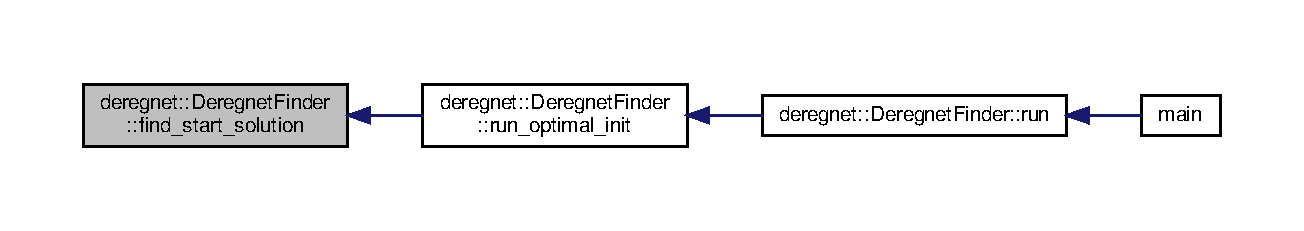
\includegraphics[width=350pt]{classderegnet_1_1DeregnetFinder_a9bca73c631c1ce679b07f1e0664abfa2_icgraph}
\end{center}
\end{figure}
\mbox{\Hypertarget{classderegnet_1_1DeregnetFinder_a1b7a50c77d09000e2d80b39025d67393}\label{classderegnet_1_1DeregnetFinder_a1b7a50c77d09000e2d80b39025d67393}} 
\index{deregnet\+::\+Deregnet\+Finder@{deregnet\+::\+Deregnet\+Finder}!find\+\_\+start\+\_\+solution@{find\+\_\+start\+\_\+solution}}
\index{find\+\_\+start\+\_\+solution@{find\+\_\+start\+\_\+solution}!deregnet\+::\+Deregnet\+Finder@{deregnet\+::\+Deregnet\+Finder}}
\subsubsection{\texorpdfstring{find\+\_\+start\+\_\+solution()}{find\_start\_solution()}\hspace{0.1cm}{\footnotesize\ttfamily [2/3]}}
{\footnotesize\ttfamily template$<$$>$ \\
void \hyperlink{classderegnet_1_1DeregnetFinder}{deregnet\+::\+Deregnet\+Finder}$<$ G\+R\+B\+Model, \hyperlink{classderegnet_1_1DrgntData}{Drgnt\+Data} $>$\+::find\+\_\+start\+\_\+solution (\begin{DoxyParamCaption}\item[{std\+::pair$<$ \hyperlink{namespacederegnet_a744bad34f2de9856d36715a445f027f3}{Node}, std\+::set$<$ \hyperlink{namespacederegnet_a744bad34f2de9856d36715a445f027f3}{Node} $>$$>$ $\ast$$\ast$}]{start\+\_\+solution }\end{DoxyParamCaption})\hspace{0.3cm}{\ttfamily [inline]}}



Definition at line 318 of file Deregnet\+Finder.\+hpp.



References deregnet\+::\+Deregnet\+Finder$<$ Model\+Type, Data $>$\+::data, deregnet\+::\+Deregnet\+Data\+::exclude, deregnet\+::\+Deregnet\+Data\+::graph, deregnet\+::\+Deregnet\+Data\+::model\+\_\+sense, deregnet\+::\+Deregnet\+Data\+::receptors, deregnet\+::\+Deregnet\+Data\+::root, and deregnet\+::\+Deregnet\+Data\+::score.


\begin{DoxyCode}
319                                                                                               \{
320     std::function<bool(double, double)> cmp;
321     \textcolor{comment}{// Adjust comparison function based on whether to minimize or maximize}
322     \textcolor{keywordflow}{if} (\hyperlink{classderegnet_1_1DeregnetFinder_ab158f2a6bb7f39ed3d6e4a9ffe568232}{data}->\hyperlink{classderegnet_1_1DeregnetData_ac3918536b5423facf0ac155997703c52}{model\_sense} == \textcolor{stringliteral}{"min"}) cmp = std::greater<double>();
323     \textcolor{keywordflow}{else} cmp = std::less<double>();
324     \textcolor{comment}{// Try to find start solution and when successful register it}
325     StartHeuristic heuristic(\hyperlink{classderegnet_1_1DeregnetFinder_ab158f2a6bb7f39ed3d6e4a9ffe568232}{data}->\hyperlink{classderegnet_1_1DeregnetData_ab76d30fa2ef87099faecb31e3f95b6d6}{graph},
326                              \hyperlink{classderegnet_1_1DeregnetFinder_ab158f2a6bb7f39ed3d6e4a9ffe568232}{data}->\hyperlink{classderegnet_1_1DeregnetData_a32970c8f43eb8be313ad08d829223b1f}{score},
327                              \hyperlink{classderegnet_1_1DeregnetFinder_ab158f2a6bb7f39ed3d6e4a9ffe568232}{data}->\hyperlink{classderegnet_1_1DeregnetData_a51a22fd88f929b1b1a00edb409b4cd55}{root},
328                              \hyperlink{classderegnet_1_1DeregnetFinder_ab158f2a6bb7f39ed3d6e4a9ffe568232}{data}->\hyperlink{classderegnet_1_1DeregnetData_a8e4398e6ece11ef87767914c6f2c304d}{exclude},
329                              \hyperlink{classderegnet_1_1DeregnetFinder_ab158f2a6bb7f39ed3d6e4a9ffe568232}{data}->\hyperlink{classderegnet_1_1DeregnetData_a470cc9f84741c59897ab1e7a3daa1205}{receptors},
330                              cmp,
331                              \hyperlink{classderegnet_1_1DeregnetFinder_ab158f2a6bb7f39ed3d6e4a9ffe568232}{data}->size);
332     \textcolor{keywordflow}{if} (heuristic.run())
333         *start\_solution = heuristic.getStartSolution();
334 \}
\end{DoxyCode}
\mbox{\Hypertarget{classderegnet_1_1DeregnetFinder_a6a5305626ad5039e294fa2f6bd3b4b74}\label{classderegnet_1_1DeregnetFinder_a6a5305626ad5039e294fa2f6bd3b4b74}} 
\index{deregnet\+::\+Deregnet\+Finder@{deregnet\+::\+Deregnet\+Finder}!find\+\_\+start\+\_\+solution@{find\+\_\+start\+\_\+solution}}
\index{find\+\_\+start\+\_\+solution@{find\+\_\+start\+\_\+solution}!deregnet\+::\+Deregnet\+Finder@{deregnet\+::\+Deregnet\+Finder}}
\subsubsection{\texorpdfstring{find\+\_\+start\+\_\+solution()}{find\_start\_solution()}\hspace{0.1cm}{\footnotesize\ttfamily [3/3]}}
{\footnotesize\ttfamily template$<$$>$ \\
void \hyperlink{classderegnet_1_1DeregnetFinder}{deregnet\+::\+Deregnet\+Finder}$<$ \hyperlink{namespacederegnet_a31759ad43b8b9641205bcf69b09f10c5}{F\+M\+I\+LP}, \hyperlink{classderegnet_1_1AvgdrgntData}{Avgdrgnt\+Data} $>$\+::find\+\_\+start\+\_\+solution (\begin{DoxyParamCaption}\item[{std\+::pair$<$ \hyperlink{namespacederegnet_a744bad34f2de9856d36715a445f027f3}{Node}, std\+::set$<$ \hyperlink{namespacederegnet_a744bad34f2de9856d36715a445f027f3}{Node} $>$$>$ $\ast$$\ast$}]{start\+\_\+solution }\end{DoxyParamCaption})\hspace{0.3cm}{\ttfamily [inline]}}



Definition at line 338 of file Deregnet\+Finder.\+hpp.



References deregnet\+::\+Deregnet\+Finder$<$ Model\+Type, Data $>$\+::data, deregnet\+::\+Deregnet\+Data\+::exclude, deregnet\+::\+Deregnet\+Data\+::graph, deregnet\+::\+Avgdrgnt\+Data\+::max\+\_\+size, deregnet\+::\+Avgdrgnt\+Data\+::min\+\_\+size, deregnet\+::\+Deregnet\+Data\+::model\+\_\+sense, deregnet\+::\+Deregnet\+Data\+::receptors, deregnet\+::\+Deregnet\+Data\+::root, and deregnet\+::\+Deregnet\+Data\+::score.


\begin{DoxyCode}
339                                                                                               \{
340 
341 
342     std::function<bool(double, double)> cmp;
343     \textcolor{comment}{// Adjust comparison function based on whether to minimize or maximize}
344     \textcolor{keywordflow}{if} (\hyperlink{classderegnet_1_1DeregnetFinder_ab158f2a6bb7f39ed3d6e4a9ffe568232}{data}->\hyperlink{classderegnet_1_1DeregnetData_ac3918536b5423facf0ac155997703c52}{model\_sense} == \textcolor{stringliteral}{"min"}) cmp = std::greater<double>();
345     \textcolor{keywordflow}{else} cmp = std::less<double>();
346     \textcolor{comment}{// Try to find start solution and when successful register it}
347     AvgStartHeuristic heuristic(\hyperlink{classderegnet_1_1DeregnetFinder_ab158f2a6bb7f39ed3d6e4a9ffe568232}{data}->\hyperlink{classderegnet_1_1DeregnetData_ab76d30fa2ef87099faecb31e3f95b6d6}{graph},
348                                 \hyperlink{classderegnet_1_1DeregnetFinder_ab158f2a6bb7f39ed3d6e4a9ffe568232}{data}->\hyperlink{classderegnet_1_1DeregnetData_a32970c8f43eb8be313ad08d829223b1f}{score},
349                                 \hyperlink{classderegnet_1_1DeregnetFinder_ab158f2a6bb7f39ed3d6e4a9ffe568232}{data}->\hyperlink{classderegnet_1_1DeregnetData_a51a22fd88f929b1b1a00edb409b4cd55}{root},
350                                 \hyperlink{classderegnet_1_1DeregnetFinder_ab158f2a6bb7f39ed3d6e4a9ffe568232}{data}->\hyperlink{classderegnet_1_1DeregnetData_a8e4398e6ece11ef87767914c6f2c304d}{exclude},
351                                 \hyperlink{classderegnet_1_1DeregnetFinder_ab158f2a6bb7f39ed3d6e4a9ffe568232}{data}->\hyperlink{classderegnet_1_1DeregnetData_a470cc9f84741c59897ab1e7a3daa1205}{receptors},
352                                 cmp,
353                                 \hyperlink{classderegnet_1_1DeregnetFinder_ab158f2a6bb7f39ed3d6e4a9ffe568232}{data}->\hyperlink{classderegnet_1_1AvgdrgntData_a733e0cd627433fca043a7f9b70af18c3}{min\_size},
354                                 \hyperlink{classderegnet_1_1DeregnetFinder_ab158f2a6bb7f39ed3d6e4a9ffe568232}{data}->\hyperlink{classderegnet_1_1AvgdrgntData_a9e844158e12d5e1c4d519c492cffeb17}{max\_size});
355     \textcolor{keywordflow}{if} (heuristic.run())
356         *start\_solution = heuristic.getStartSolution();
357 \}
\end{DoxyCode}
\mbox{\Hypertarget{classderegnet_1_1DeregnetFinder_a85fcde1dddbfd03ffc4ae8d244b4fc72}\label{classderegnet_1_1DeregnetFinder_a85fcde1dddbfd03ffc4ae8d244b4fc72}} 
\index{deregnet\+::\+Deregnet\+Finder@{deregnet\+::\+Deregnet\+Finder}!find\+\_\+suboptimal\+\_\+start\+\_\+solution@{find\+\_\+suboptimal\+\_\+start\+\_\+solution}}
\index{find\+\_\+suboptimal\+\_\+start\+\_\+solution@{find\+\_\+suboptimal\+\_\+start\+\_\+solution}!deregnet\+::\+Deregnet\+Finder@{deregnet\+::\+Deregnet\+Finder}}
\subsubsection{\texorpdfstring{find\+\_\+suboptimal\+\_\+start\+\_\+solution()}{find\_suboptimal\_start\_solution()}\hspace{0.1cm}{\footnotesize\ttfamily [1/3]}}
{\footnotesize\ttfamily template$<$typename Model\+Type, typename Data$>$ \\
void \hyperlink{classderegnet_1_1DeregnetFinder}{deregnet\+::\+Deregnet\+Finder}$<$ Model\+Type, \hyperlink{avgdrgnt_8cpp_a1d1235306db276e9b36acba1db1509e8}{Data} $>$\+::find\+\_\+suboptimal\+\_\+start\+\_\+solution (\begin{DoxyParamCaption}\item[{std\+::pair$<$ \hyperlink{namespacederegnet_a744bad34f2de9856d36715a445f027f3}{Node}, std\+::set$<$ \hyperlink{namespacederegnet_a744bad34f2de9856d36715a445f027f3}{Node} $>$$>$ $\ast$$\ast$}]{start\+\_\+solution,  }\item[{std\+::set$<$ std\+::string $>$ $\ast$}]{nodes\+\_\+so\+\_\+far }\end{DoxyParamCaption})}



Finds a heuristic suboptimal start solution. 



Referenced by deregnet\+::\+Deregnet\+Finder$<$ Model\+Type, Data $>$\+::run\+\_\+suboptimal\+\_\+init().

Here is the caller graph for this function\+:\nopagebreak
\begin{figure}[H]
\begin{center}
\leavevmode
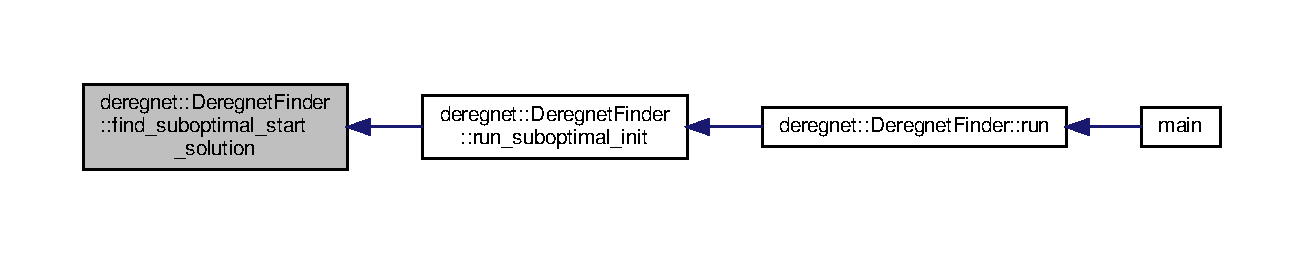
\includegraphics[width=350pt]{classderegnet_1_1DeregnetFinder_a85fcde1dddbfd03ffc4ae8d244b4fc72_icgraph}
\end{center}
\end{figure}
\mbox{\Hypertarget{classderegnet_1_1DeregnetFinder_a42eca7055ed54197e27df7bd70271a13}\label{classderegnet_1_1DeregnetFinder_a42eca7055ed54197e27df7bd70271a13}} 
\index{deregnet\+::\+Deregnet\+Finder@{deregnet\+::\+Deregnet\+Finder}!find\+\_\+suboptimal\+\_\+start\+\_\+solution@{find\+\_\+suboptimal\+\_\+start\+\_\+solution}}
\index{find\+\_\+suboptimal\+\_\+start\+\_\+solution@{find\+\_\+suboptimal\+\_\+start\+\_\+solution}!deregnet\+::\+Deregnet\+Finder@{deregnet\+::\+Deregnet\+Finder}}
\subsubsection{\texorpdfstring{find\+\_\+suboptimal\+\_\+start\+\_\+solution()}{find\_suboptimal\_start\_solution()}\hspace{0.1cm}{\footnotesize\ttfamily [2/3]}}
{\footnotesize\ttfamily template$<$$>$ \\
void \hyperlink{classderegnet_1_1DeregnetFinder}{deregnet\+::\+Deregnet\+Finder}$<$ G\+R\+B\+Model, \hyperlink{classderegnet_1_1DrgntData}{Drgnt\+Data} $>$\+::find\+\_\+suboptimal\+\_\+start\+\_\+solution (\begin{DoxyParamCaption}\item[{std\+::pair$<$ \hyperlink{namespacederegnet_a744bad34f2de9856d36715a445f027f3}{Node}, std\+::set$<$ \hyperlink{namespacederegnet_a744bad34f2de9856d36715a445f027f3}{Node} $>$$>$ $\ast$$\ast$}]{start\+\_\+solution,  }\item[{std\+::set$<$ std\+::string $>$ $\ast$}]{nodes\+\_\+so\+\_\+far }\end{DoxyParamCaption})\hspace{0.3cm}{\ttfamily [inline]}}



Definition at line 364 of file Deregnet\+Finder.\+hpp.



References deregnet\+::\+Deregnet\+Finder$<$ Model\+Type, Data $>$\+::data, deregnet\+::\+Deregnet\+Data\+::exclude, deregnet\+::\+Deregnet\+Data\+::graph, deregnet\+::\+Deregnet\+Data\+::max\+\_\+overlap, deregnet\+::\+Deregnet\+Data\+::model\+\_\+sense, deregnet\+::\+Deregnet\+Data\+::nodeid, deregnet\+::\+Deregnet\+Data\+::receptors, deregnet\+::\+Deregnet\+Data\+::root, and deregnet\+::\+Deregnet\+Data\+::score.


\begin{DoxyCode}
365                                                                                                           \{
366     std::function<bool(double, double)> cmp;
367     \textcolor{comment}{// Adjust comparison function based on whether to minimize or maximize}
368     \textcolor{keywordflow}{if} (\hyperlink{classderegnet_1_1DeregnetFinder_ab158f2a6bb7f39ed3d6e4a9ffe568232}{data}->\hyperlink{classderegnet_1_1DeregnetData_ac3918536b5423facf0ac155997703c52}{model\_sense} == \textcolor{stringliteral}{"min"}) cmp = std::greater<double>();
369     \textcolor{keywordflow}{else} cmp = std::less<double>();
370     \textcolor{comment}{// Try to find start solution and when successful register it}
371     SuboptimalStartHeuristic heuristic(\hyperlink{classderegnet_1_1DeregnetFinder_ab158f2a6bb7f39ed3d6e4a9ffe568232}{data}->\hyperlink{classderegnet_1_1DeregnetData_ab76d30fa2ef87099faecb31e3f95b6d6}{graph},
372                                        \hyperlink{classderegnet_1_1DeregnetFinder_ab158f2a6bb7f39ed3d6e4a9ffe568232}{data}->\hyperlink{classderegnet_1_1DeregnetData_a32970c8f43eb8be313ad08d829223b1f}{score},
373                                        \hyperlink{classderegnet_1_1DeregnetFinder_ab158f2a6bb7f39ed3d6e4a9ffe568232}{data}->\hyperlink{classderegnet_1_1DeregnetData_a51a22fd88f929b1b1a00edb409b4cd55}{root},
374                                        \hyperlink{classderegnet_1_1DeregnetFinder_ab158f2a6bb7f39ed3d6e4a9ffe568232}{data}->\hyperlink{classderegnet_1_1DeregnetData_a8e4398e6ece11ef87767914c6f2c304d}{exclude},
375                                        \hyperlink{classderegnet_1_1DeregnetFinder_ab158f2a6bb7f39ed3d6e4a9ffe568232}{data}->\hyperlink{classderegnet_1_1DeregnetData_a470cc9f84741c59897ab1e7a3daa1205}{receptors},
376                                        cmp,
377                                        \hyperlink{classderegnet_1_1DeregnetFinder_ab158f2a6bb7f39ed3d6e4a9ffe568232}{data}->\hyperlink{classderegnet_1_1DeregnetData_a3b57d7ed19c104c7fe257e17f0d2cfb5}{nodeid},
378                                        nodes\_so\_far,
379                                        \hyperlink{classderegnet_1_1DeregnetFinder_ab158f2a6bb7f39ed3d6e4a9ffe568232}{data}->\hyperlink{classderegnet_1_1DeregnetData_a43111d8664fd9db36f36f75b24ba62e9}{max\_overlap},
380                                        \hyperlink{classderegnet_1_1DeregnetFinder_ab158f2a6bb7f39ed3d6e4a9ffe568232}{data}->size);
381     \textcolor{keywordflow}{if} (heuristic.run())
382         *start\_solution = heuristic.getStartSolution();
383 \}
\end{DoxyCode}
\mbox{\Hypertarget{classderegnet_1_1DeregnetFinder_ae81ebb01d3cba09b12858bce7799e2a5}\label{classderegnet_1_1DeregnetFinder_ae81ebb01d3cba09b12858bce7799e2a5}} 
\index{deregnet\+::\+Deregnet\+Finder@{deregnet\+::\+Deregnet\+Finder}!find\+\_\+suboptimal\+\_\+start\+\_\+solution@{find\+\_\+suboptimal\+\_\+start\+\_\+solution}}
\index{find\+\_\+suboptimal\+\_\+start\+\_\+solution@{find\+\_\+suboptimal\+\_\+start\+\_\+solution}!deregnet\+::\+Deregnet\+Finder@{deregnet\+::\+Deregnet\+Finder}}
\subsubsection{\texorpdfstring{find\+\_\+suboptimal\+\_\+start\+\_\+solution()}{find\_suboptimal\_start\_solution()}\hspace{0.1cm}{\footnotesize\ttfamily [3/3]}}
{\footnotesize\ttfamily template$<$$>$ \\
void \hyperlink{classderegnet_1_1DeregnetFinder}{deregnet\+::\+Deregnet\+Finder}$<$ \hyperlink{namespacederegnet_a31759ad43b8b9641205bcf69b09f10c5}{F\+M\+I\+LP}, \hyperlink{classderegnet_1_1AvgdrgntData}{Avgdrgnt\+Data} $>$\+::find\+\_\+suboptimal\+\_\+start\+\_\+solution (\begin{DoxyParamCaption}\item[{std\+::pair$<$ \hyperlink{namespacederegnet_a744bad34f2de9856d36715a445f027f3}{Node}, std\+::set$<$ \hyperlink{namespacederegnet_a744bad34f2de9856d36715a445f027f3}{Node} $>$$>$ $\ast$$\ast$}]{start\+\_\+solution,  }\item[{std\+::set$<$ std\+::string $>$ $\ast$}]{nodes\+\_\+so\+\_\+far }\end{DoxyParamCaption})\hspace{0.3cm}{\ttfamily [inline]}}



Definition at line 387 of file Deregnet\+Finder.\+hpp.



References deregnet\+::\+Deregnet\+Finder$<$ Model\+Type, Data $>$\+::data, deregnet\+::\+Deregnet\+Data\+::exclude, deregnet\+::\+Deregnet\+Data\+::graph, deregnet\+::\+Deregnet\+Data\+::max\+\_\+overlap, deregnet\+::\+Avgdrgnt\+Data\+::max\+\_\+size, deregnet\+::\+Avgdrgnt\+Data\+::min\+\_\+size, deregnet\+::\+Deregnet\+Data\+::model\+\_\+sense, deregnet\+::\+Deregnet\+Data\+::nodeid, deregnet\+::\+Deregnet\+Data\+::receptors, deregnet\+::\+Deregnet\+Data\+::root, and deregnet\+::\+Deregnet\+Data\+::score.


\begin{DoxyCode}
388                                                                                                           \{
389 
390     std::function<bool(double, double)> cmp;
391     \textcolor{comment}{// Adjust comparison function based on whether to minimize or maximize}
392     \textcolor{keywordflow}{if} (\hyperlink{classderegnet_1_1DeregnetFinder_ab158f2a6bb7f39ed3d6e4a9ffe568232}{data}->\hyperlink{classderegnet_1_1DeregnetData_ac3918536b5423facf0ac155997703c52}{model\_sense} == \textcolor{stringliteral}{"min"}) cmp = std::greater<double>();
393     \textcolor{keywordflow}{else} cmp = std::less<double>();
394     \textcolor{comment}{// Try to find start solution and when successful register it}
395     AvgSuboptimalStartHeuristic heuristic(\hyperlink{classderegnet_1_1DeregnetFinder_ab158f2a6bb7f39ed3d6e4a9ffe568232}{data}->\hyperlink{classderegnet_1_1DeregnetData_ab76d30fa2ef87099faecb31e3f95b6d6}{graph},
396                                           \hyperlink{classderegnet_1_1DeregnetFinder_ab158f2a6bb7f39ed3d6e4a9ffe568232}{data}->\hyperlink{classderegnet_1_1DeregnetData_a32970c8f43eb8be313ad08d829223b1f}{score},
397                                           \hyperlink{classderegnet_1_1DeregnetFinder_ab158f2a6bb7f39ed3d6e4a9ffe568232}{data}->\hyperlink{classderegnet_1_1DeregnetData_a51a22fd88f929b1b1a00edb409b4cd55}{root},
398                                           \hyperlink{classderegnet_1_1DeregnetFinder_ab158f2a6bb7f39ed3d6e4a9ffe568232}{data}->\hyperlink{classderegnet_1_1DeregnetData_a8e4398e6ece11ef87767914c6f2c304d}{exclude},
399                                           \hyperlink{classderegnet_1_1DeregnetFinder_ab158f2a6bb7f39ed3d6e4a9ffe568232}{data}->\hyperlink{classderegnet_1_1DeregnetData_a470cc9f84741c59897ab1e7a3daa1205}{receptors},
400                                           cmp,
401                                           \hyperlink{classderegnet_1_1DeregnetFinder_ab158f2a6bb7f39ed3d6e4a9ffe568232}{data}->\hyperlink{classderegnet_1_1DeregnetData_a3b57d7ed19c104c7fe257e17f0d2cfb5}{nodeid},
402                                           nodes\_so\_far,
403                                           \hyperlink{classderegnet_1_1DeregnetFinder_ab158f2a6bb7f39ed3d6e4a9ffe568232}{data}->\hyperlink{classderegnet_1_1DeregnetData_a43111d8664fd9db36f36f75b24ba62e9}{max\_overlap},
404                                           \hyperlink{classderegnet_1_1DeregnetFinder_ab158f2a6bb7f39ed3d6e4a9ffe568232}{data}->\hyperlink{classderegnet_1_1AvgdrgntData_a733e0cd627433fca043a7f9b70af18c3}{min\_size},
405                                           \hyperlink{classderegnet_1_1DeregnetFinder_ab158f2a6bb7f39ed3d6e4a9ffe568232}{data}->\hyperlink{classderegnet_1_1AvgdrgntData_a9e844158e12d5e1c4d519c492cffeb17}{max\_size});
406     \textcolor{keywordflow}{if} (heuristic.run())
407         *start\_solution = heuristic.getStartSolution();
408 
409 \}
\end{DoxyCode}
\mbox{\Hypertarget{classderegnet_1_1DeregnetFinder_a1a6119b306b54ff44d8c78f34fc037ab}\label{classderegnet_1_1DeregnetFinder_a1a6119b306b54ff44d8c78f34fc037ab}} 
\index{deregnet\+::\+Deregnet\+Finder@{deregnet\+::\+Deregnet\+Finder}!run@{run}}
\index{run@{run}!deregnet\+::\+Deregnet\+Finder@{deregnet\+::\+Deregnet\+Finder}}
\subsubsection{\texorpdfstring{run()}{run()}}
{\footnotesize\ttfamily template$<$typename Model\+Type , typename Data $>$ \\
std\+::vector$<$ \hyperlink{structderegnet_1_1Subgraph}{Subgraph} $>$ \hyperlink{classderegnet_1_1DeregnetFinder}{deregnet\+::\+Deregnet\+Finder}$<$ Model\+Type, \hyperlink{avgdrgnt_8cpp_a1d1235306db276e9b36acba1db1509e8}{Data} $>$\+::run (\begin{DoxyParamCaption}{ }\end{DoxyParamCaption})}



Method which finds the subgraphs. 

This method finds subgraphs as specified on instantiation of the \hyperlink{classderegnet_1_1DeregnetFinder}{Deregnet\+Finder} instance. You get back a vector with the subgraphs.

\begin{DoxyReturn}{Returns}
Vector containing the the subgraphs 
\end{DoxyReturn}


Definition at line 252 of file Deregnet\+Finder.\+hpp.



References deregnet\+::\+Deregnet\+Finder$<$ Model\+Type, Data $>$\+::data, deregnet\+::\+Deregnet\+Finder$<$ Model\+Type, Data $>$\+::model, deregnet\+::\+Deregnet\+Data\+::num\+\_\+subopt\+\_\+iter, deregnet\+::\+Deregnet\+Finder$<$ Model\+Type, Data $>$\+::run\+\_\+optimal\+\_\+init(), deregnet\+::\+Deregnet\+Finder$<$ Model\+Type, Data $>$\+::run\+\_\+optimal\+\_\+windup(), deregnet\+::\+Deregnet\+Finder$<$ Model\+Type, Data $>$\+::run\+\_\+suboptimal\+\_\+init(), and deregnet\+::\+Deregnet\+Finder$<$ Model\+Type, Data $>$\+::run\+\_\+suboptimal\+\_\+windup().



Referenced by main().


\begin{DoxyCode}
252                                                          \{
253     std::pair<Node, std::set<Node>>* start\_solution \{ \textcolor{keyword}{nullptr} \};      \textcolor{comment}{// potential heuristic start solution}
254     \textcolor{comment}{// find optimal subgraph}
255     \hyperlink{classderegnet_1_1DeregnetFinder_ae0335349d6a60ee204d10bf8b7366cfa}{run\_optimal\_init}(&start\_solution);                                \textcolor{comment}{// construct model,
       etc.}
256 \textcolor{comment}{/*}
257 \textcolor{comment}{    std::ofstream file;}
258 \textcolor{comment}{    file.open("heuristic\_start.nodes");}
259 \textcolor{comment}{    for (auto v : start\_solution->second)}
260 \textcolor{comment}{        file << (*data->nodeid)[v] << "\(\backslash\)n";}
261 \textcolor{comment}{    file.close();}
262 \textcolor{comment}{*/}
263     std::vector<Subgraph> subgraphs;                                  \textcolor{comment}{// data structure for found subgraphs}
264     \textcolor{keywordtype}{bool} solve\_successful \{ \hyperlink{classderegnet_1_1DeregnetFinder_ad922d8e38124b4c75daac29a928fcf5b}{model}->solve(start\_solution) \};           \textcolor{comment}{// try to find optimal solution}
265     \hyperlink{classderegnet_1_1DeregnetFinder_a92610c1444ba271820e64d224ec64bb7}{run\_optimal\_windup}(solve\_successful, &subgraphs);                 \textcolor{comment}{// handle result of
       optimal solution attempt}
266     \textcolor{comment}{// find suboptimal subgraphs}
267     std::set<std::string> nodes\_so\_far \{ subgraphs.back().nodes \};    \textcolor{comment}{// tracking nodes contained in some
       already found subgraph}
268     \textcolor{keywordflow}{for} (\textcolor{keywordtype}{int} i = 0; i < \hyperlink{classderegnet_1_1DeregnetFinder_ab158f2a6bb7f39ed3d6e4a9ffe568232}{data}->\hyperlink{classderegnet_1_1DeregnetData_adb7428cd99112156ae9f80187af9ebbe}{num\_subopt\_iter}; ++i) \{
269         start\_solution = \textcolor{keyword}{nullptr};                                     \textcolor{comment}{// reset to NULL ... Where does the
       previous one go? Memory leak?}
270         \hyperlink{classderegnet_1_1DeregnetFinder_ad996cee997a5db4e09016a6f725a6701}{run\_suboptimal\_init}(&start\_solution, &nodes\_so\_far);          \textcolor{comment}{// adapt model for
       finding next suboptimal, etc.}
271         solve\_successful = \hyperlink{classderegnet_1_1DeregnetFinder_ad922d8e38124b4c75daac29a928fcf5b}{model}->solve(start\_solution);              \textcolor{comment}{// try to find next suboptimal
       solution}
272         \textcolor{keywordflow}{if} (!\hyperlink{classderegnet_1_1DeregnetFinder_a4021d92d787877187a24dcbaf0c1bad1}{run\_suboptimal\_windup}(solve\_successful, &subgraphs, &nodes\_so\_far, i))   
         \textcolor{comment}{// once no suboptimal subgraph could be found, do not try again ;)}
273             \textcolor{keywordflow}{break};
274     \}
275     \textcolor{keywordflow}{return} subgraphs;
276 \}
\end{DoxyCode}
Here is the call graph for this function\+:\nopagebreak
\begin{figure}[H]
\begin{center}
\leavevmode
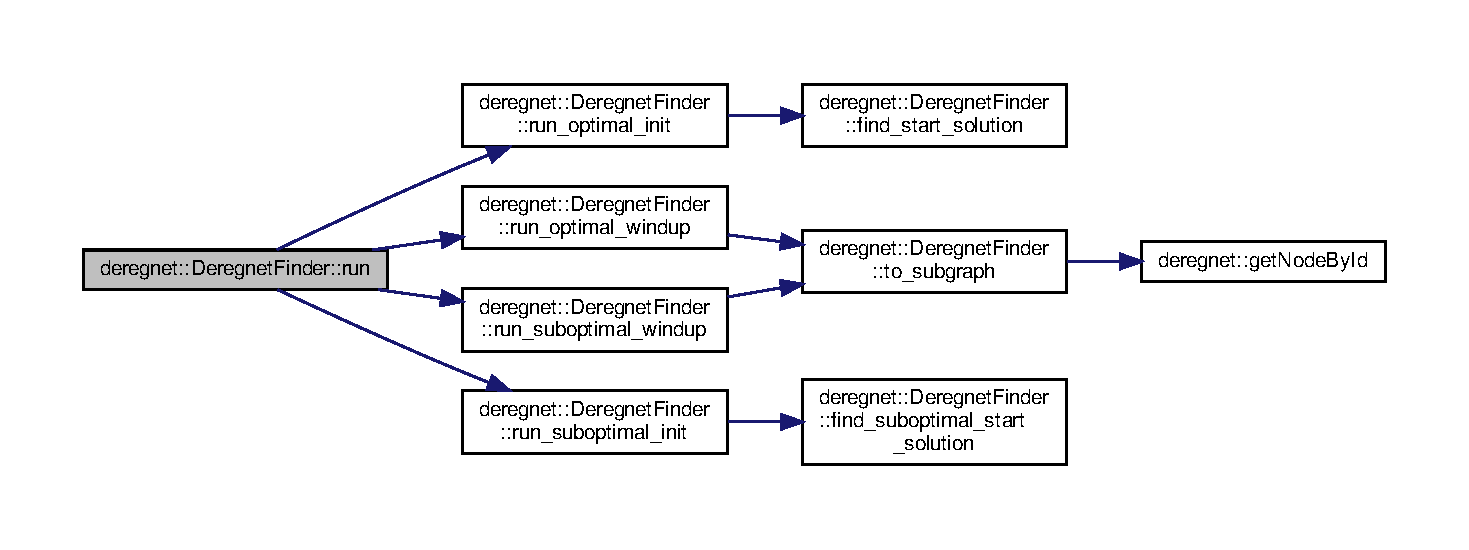
\includegraphics[width=350pt]{classderegnet_1_1DeregnetFinder_a1a6119b306b54ff44d8c78f34fc037ab_cgraph}
\end{center}
\end{figure}
Here is the caller graph for this function\+:\nopagebreak
\begin{figure}[H]
\begin{center}
\leavevmode
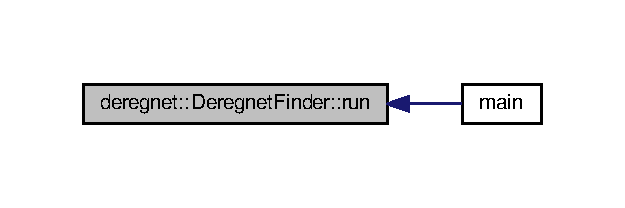
\includegraphics[width=300pt]{classderegnet_1_1DeregnetFinder_a1a6119b306b54ff44d8c78f34fc037ab_icgraph}
\end{center}
\end{figure}
\mbox{\Hypertarget{classderegnet_1_1DeregnetFinder_ae0335349d6a60ee204d10bf8b7366cfa}\label{classderegnet_1_1DeregnetFinder_ae0335349d6a60ee204d10bf8b7366cfa}} 
\index{deregnet\+::\+Deregnet\+Finder@{deregnet\+::\+Deregnet\+Finder}!run\+\_\+optimal\+\_\+init@{run\+\_\+optimal\+\_\+init}}
\index{run\+\_\+optimal\+\_\+init@{run\+\_\+optimal\+\_\+init}!deregnet\+::\+Deregnet\+Finder@{deregnet\+::\+Deregnet\+Finder}}
\subsubsection{\texorpdfstring{run\+\_\+optimal\+\_\+init()}{run\_optimal\_init()}}
{\footnotesize\ttfamily template$<$typename Model\+Type, typename Data$>$ \\
void \hyperlink{classderegnet_1_1DeregnetFinder}{deregnet\+::\+Deregnet\+Finder}$<$ Model\+Type, \hyperlink{avgdrgnt_8cpp_a1d1235306db276e9b36acba1db1509e8}{Data} $>$\+::run\+\_\+optimal\+\_\+init (\begin{DoxyParamCaption}\item[{std\+::pair$<$ \hyperlink{namespacederegnet_a744bad34f2de9856d36715a445f027f3}{Node}, std\+::set$<$ \hyperlink{namespacederegnet_a744bad34f2de9856d36715a445f027f3}{Node} $>$$>$ $\ast$$\ast$}]{start\+\_\+solution }\end{DoxyParamCaption})\hspace{0.3cm}{\ttfamily [private]}}



Preparation for finding the optimal subgraph. 



Definition at line 173 of file Deregnet\+Finder.\+hpp.



References deregnet\+::\+Deregnet\+Finder$<$ Model\+Type, Data $>$\+::data, deregnet\+::\+Deregnet\+Data\+::exclude, deregnet\+::\+Deregnet\+Finder$<$ Model\+Type, Data $>$\+::find\+\_\+start\+\_\+solution(), deregnet\+::\+Deregnet\+Data\+::include, deregnet\+::\+Deregnet\+Finder$<$ Model\+Type, Data $>$\+::model, deregnet\+::\+Deregnet\+Data\+::receptors, deregnet\+::\+Deregnet\+Data\+::root, deregnet\+::\+Deregnet\+Data\+::start\+\_\+heuristic, and deregnet\+::\+Deregnet\+Data\+::terminals.



Referenced by deregnet\+::\+Deregnet\+Finder$<$ Model\+Type, Data $>$\+::run().


\begin{DoxyCode}
173                                                                                                     \{
174     \hyperlink{classderegnet_1_1DeregnetFinder_ad922d8e38124b4c75daac29a928fcf5b}{model}->createVariables();       \textcolor{comment}{// create binary variables corresponding to the nodes}
175     \hyperlink{classderegnet_1_1DeregnetFinder_ad922d8e38124b4c75daac29a928fcf5b}{model}->addBaseConstraints();    \textcolor{comment}{// add base constraints to the model, ie connectivity etc.}
176     \textcolor{comment}{// add optional constraints (ie. include, exclude, receptor and/or terminal constraints)}
177     \textcolor{keywordflow}{if} (\hyperlink{classderegnet_1_1DeregnetFinder_ab158f2a6bb7f39ed3d6e4a9ffe568232}{data}->\hyperlink{classderegnet_1_1DeregnetData_a438d16e60be5d119d174aa039f070ab2}{include})
178         \hyperlink{classderegnet_1_1DeregnetFinder_ad922d8e38124b4c75daac29a928fcf5b}{model}->addIncludeConstraints();   \textcolor{comment}{// which nodes to include in the subgraph, no matter what}
179     \textcolor{keywordflow}{if} (\hyperlink{classderegnet_1_1DeregnetFinder_ab158f2a6bb7f39ed3d6e4a9ffe568232}{data}->\hyperlink{classderegnet_1_1DeregnetData_a8e4398e6ece11ef87767914c6f2c304d}{exclude})
180         \hyperlink{classderegnet_1_1DeregnetFinder_ad922d8e38124b4c75daac29a928fcf5b}{model}->addExcludeConstraints();   \textcolor{comment}{// which nodes to exclude from the subgraph, no matter what}
181     \textcolor{keywordflow}{if} (\hyperlink{classderegnet_1_1DeregnetFinder_ab158f2a6bb7f39ed3d6e4a9ffe568232}{data}->\hyperlink{classderegnet_1_1DeregnetData_a470cc9f84741c59897ab1e7a3daa1205}{receptors} && !\hyperlink{classderegnet_1_1DeregnetFinder_ab158f2a6bb7f39ed3d6e4a9ffe568232}{data}->\hyperlink{classderegnet_1_1DeregnetData_a51a22fd88f929b1b1a00edb409b4cd55}{root})
182         \hyperlink{classderegnet_1_1DeregnetFinder_ad922d8e38124b4c75daac29a928fcf5b}{model}->addReceptorConstraints();  \textcolor{comment}{// how to handle nodes which are 'receptors'}
183     \textcolor{keywordflow}{if} (\hyperlink{classderegnet_1_1DeregnetFinder_ab158f2a6bb7f39ed3d6e4a9ffe568232}{data}->\hyperlink{classderegnet_1_1DeregnetData_a1fe559c6056cd411647f836849e4b0da}{terminals})
184         \hyperlink{classderegnet_1_1DeregnetFinder_ad922d8e38124b4c75daac29a928fcf5b}{model}->addTerminalConstraints();  \textcolor{comment}{// how to handle nodes which are 'temrinals'}
185     \textcolor{comment}{// optionally find heuristic start solution by greedy algorithm}
186     \textcolor{keywordflow}{if} (\hyperlink{classderegnet_1_1DeregnetFinder_ab158f2a6bb7f39ed3d6e4a9ffe568232}{data}->\hyperlink{classderegnet_1_1DeregnetData_abac721360704af5615f7ff84b183eebd}{start\_heuristic})
187         \hyperlink{classderegnet_1_1DeregnetFinder_a9bca73c631c1ce679b07f1e0664abfa2}{find\_start\_solution}(start\_solution);
188     \textcolor{comment}{// in case a heuristic start solution was specfied but none was found, issue a warning.}
189     \textcolor{comment}{// TODO: not necessarily always to std::cout ...}
190     \textcolor{keywordflow}{if} (\hyperlink{classderegnet_1_1DeregnetFinder_ab158f2a6bb7f39ed3d6e4a9ffe568232}{data}->\hyperlink{classderegnet_1_1DeregnetData_abac721360704af5615f7ff84b183eebd}{start\_heuristic} && !(*start\_solution))
191         std::cout << \textcolor{stringliteral}{"No heuristic start solution found.\(\backslash\)n"} << std::endl;
192 \}
\end{DoxyCode}
Here is the call graph for this function\+:\nopagebreak
\begin{figure}[H]
\begin{center}
\leavevmode
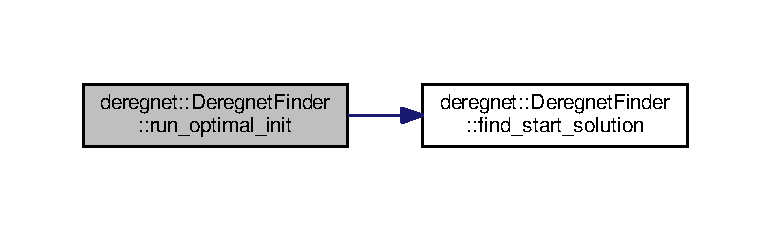
\includegraphics[width=350pt]{classderegnet_1_1DeregnetFinder_ae0335349d6a60ee204d10bf8b7366cfa_cgraph}
\end{center}
\end{figure}
Here is the caller graph for this function\+:\nopagebreak
\begin{figure}[H]
\begin{center}
\leavevmode
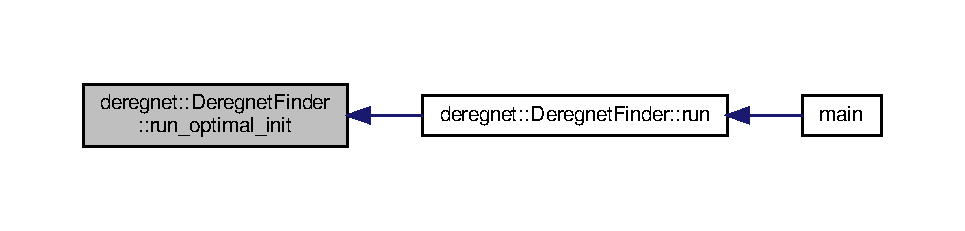
\includegraphics[width=350pt]{classderegnet_1_1DeregnetFinder_ae0335349d6a60ee204d10bf8b7366cfa_icgraph}
\end{center}
\end{figure}
\mbox{\Hypertarget{classderegnet_1_1DeregnetFinder_a92610c1444ba271820e64d224ec64bb7}\label{classderegnet_1_1DeregnetFinder_a92610c1444ba271820e64d224ec64bb7}} 
\index{deregnet\+::\+Deregnet\+Finder@{deregnet\+::\+Deregnet\+Finder}!run\+\_\+optimal\+\_\+windup@{run\+\_\+optimal\+\_\+windup}}
\index{run\+\_\+optimal\+\_\+windup@{run\+\_\+optimal\+\_\+windup}!deregnet\+::\+Deregnet\+Finder@{deregnet\+::\+Deregnet\+Finder}}
\subsubsection{\texorpdfstring{run\+\_\+optimal\+\_\+windup()}{run\_optimal\_windup()}}
{\footnotesize\ttfamily template$<$typename Model\+Type , typename Data $>$ \\
void \hyperlink{classderegnet_1_1DeregnetFinder}{deregnet\+::\+Deregnet\+Finder}$<$ Model\+Type, \hyperlink{avgdrgnt_8cpp_a1d1235306db276e9b36acba1db1509e8}{Data} $>$\+::run\+\_\+optimal\+\_\+windup (\begin{DoxyParamCaption}\item[{bool}]{solve\+\_\+successful,  }\item[{std\+::vector$<$ \hyperlink{structderegnet_1_1Subgraph}{Subgraph} $>$ $\ast$}]{subgraphs }\end{DoxyParamCaption})\hspace{0.3cm}{\ttfamily [private]}}



Post-\/processing after attempt to find optimal subgraph. 



Definition at line 196 of file Deregnet\+Finder.\+hpp.



References deregnet\+::\+Deregnet\+Finder$<$ Model\+Type, Data $>$\+::model, N\+O\+\_\+\+O\+P\+T\+I\+M\+A\+L\+\_\+\+S\+U\+B\+G\+R\+A\+P\+H\+\_\+\+F\+O\+U\+ND, and deregnet\+::\+Deregnet\+Finder$<$ Model\+Type, Data $>$\+::to\+\_\+subgraph().



Referenced by deregnet\+::\+Deregnet\+Finder$<$ Model\+Type, Data $>$\+::run().


\begin{DoxyCode}
196                                                                                                            
         \{
197     \textcolor{comment}{// if a solution was found update subgraphs data structure}
198     \textcolor{keywordflow}{if} ( solve\_successful ) \{
199         subgraphs->push\_back ( \hyperlink{classderegnet_1_1DeregnetFinder_a681d5e2506f9b6075ab36e742a360328}{to\_subgraph}( \hyperlink{classderegnet_1_1DeregnetFinder_ad922d8e38124b4c75daac29a928fcf5b}{model}->getCurrentSolution(), \textcolor{stringliteral}{"optimal"} ) );
200     \}
201     \textcolor{comment}{// if no solution was found, issue a message and end the program}
202     \textcolor{comment}{// TODO: not necessarily always to std::cerr}
203     \textcolor{comment}{// TODO: exit normally and handle issue in normal program flow?}
204     \textcolor{keywordflow}{else} \{
205         std::cerr << \textcolor{stringliteral}{"No optimal subgraph could be found."} << std::endl;
206         exit(\hyperlink{DeregnetData_8hpp_a4cfde67e3f13f361cd54de13be284610}{NO\_OPTIMAL\_SUBGRAPH\_FOUND});
207     \}
208 \}
\end{DoxyCode}
Here is the call graph for this function\+:\nopagebreak
\begin{figure}[H]
\begin{center}
\leavevmode
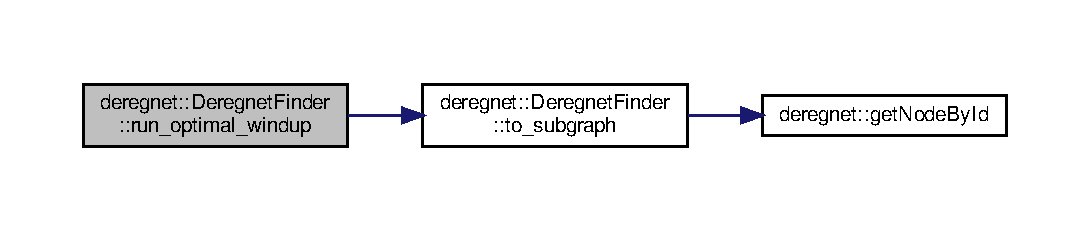
\includegraphics[width=350pt]{classderegnet_1_1DeregnetFinder_a92610c1444ba271820e64d224ec64bb7_cgraph}
\end{center}
\end{figure}
Here is the caller graph for this function\+:\nopagebreak
\begin{figure}[H]
\begin{center}
\leavevmode
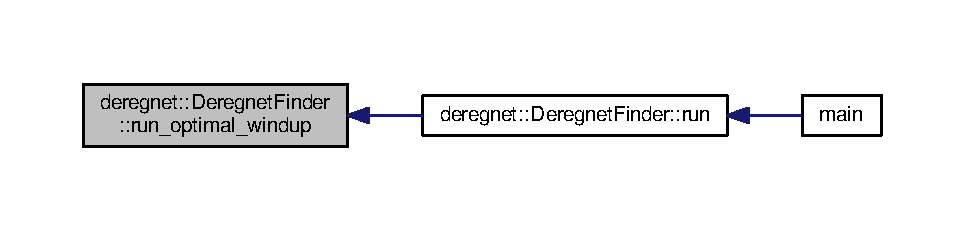
\includegraphics[width=350pt]{classderegnet_1_1DeregnetFinder_a92610c1444ba271820e64d224ec64bb7_icgraph}
\end{center}
\end{figure}
\mbox{\Hypertarget{classderegnet_1_1DeregnetFinder_ad996cee997a5db4e09016a6f725a6701}\label{classderegnet_1_1DeregnetFinder_ad996cee997a5db4e09016a6f725a6701}} 
\index{deregnet\+::\+Deregnet\+Finder@{deregnet\+::\+Deregnet\+Finder}!run\+\_\+suboptimal\+\_\+init@{run\+\_\+suboptimal\+\_\+init}}
\index{run\+\_\+suboptimal\+\_\+init@{run\+\_\+suboptimal\+\_\+init}!deregnet\+::\+Deregnet\+Finder@{deregnet\+::\+Deregnet\+Finder}}
\subsubsection{\texorpdfstring{run\+\_\+suboptimal\+\_\+init()}{run\_suboptimal\_init()}}
{\footnotesize\ttfamily template$<$typename Model\+Type , typename Data $>$ \\
void \hyperlink{classderegnet_1_1DeregnetFinder}{deregnet\+::\+Deregnet\+Finder}$<$ Model\+Type, \hyperlink{avgdrgnt_8cpp_a1d1235306db276e9b36acba1db1509e8}{Data} $>$\+::run\+\_\+suboptimal\+\_\+init (\begin{DoxyParamCaption}\item[{std\+::pair$<$ \hyperlink{namespacederegnet_a744bad34f2de9856d36715a445f027f3}{Node}, std\+::set$<$ \hyperlink{namespacederegnet_a744bad34f2de9856d36715a445f027f3}{Node} $>$ $>$ $\ast$$\ast$}]{start\+\_\+solution,  }\item[{std\+::set$<$ std\+::string $>$ $\ast$}]{nodes\+\_\+so\+\_\+far }\end{DoxyParamCaption})\hspace{0.3cm}{\ttfamily [private]}}



Perparation for finding suboptimal subgraphs. 



Definition at line 212 of file Deregnet\+Finder.\+hpp.



References deregnet\+::\+Deregnet\+Finder$<$ Model\+Type, Data $>$\+::data, deregnet\+::\+Deregnet\+Finder$<$ Model\+Type, Data $>$\+::find\+\_\+suboptimal\+\_\+start\+\_\+solution(), deregnet\+::\+Deregnet\+Finder$<$ Model\+Type, Data $>$\+::model, and deregnet\+::\+Deregnet\+Data\+::start\+\_\+heuristic.



Referenced by deregnet\+::\+Deregnet\+Finder$<$ Model\+Type, Data $>$\+::run().


\begin{DoxyCode}
213                                                                                            \{
214     \textcolor{comment}{// make sure only a certain fraction of nodes contained in some already found subgraph}
215     \textcolor{comment}{// will be contained this subgraph}
216     \hyperlink{classderegnet_1_1DeregnetFinder_ad922d8e38124b4c75daac29a928fcf5b}{model}->addSuboptimalityConstraint(*nodes\_so\_far);  
217     \textcolor{comment}{// optionally find heuristic start solution by greedy algorithm}
218     \textcolor{keywordflow}{if} (\hyperlink{classderegnet_1_1DeregnetFinder_ab158f2a6bb7f39ed3d6e4a9ffe568232}{data}->\hyperlink{classderegnet_1_1DeregnetData_abac721360704af5615f7ff84b183eebd}{start\_heuristic})
219         \hyperlink{classderegnet_1_1DeregnetFinder_a85fcde1dddbfd03ffc4ae8d244b4fc72}{find\_suboptimal\_start\_solution}(start\_solution, nodes\_so\_far);
220     \textcolor{comment}{// in case a heuristic start solution was specfied but none was found, issue a warning.}
221     \textcolor{comment}{// TODO: not necessarily always to std::cout ...}
222     \textcolor{keywordflow}{if} (\hyperlink{classderegnet_1_1DeregnetFinder_ab158f2a6bb7f39ed3d6e4a9ffe568232}{data}->\hyperlink{classderegnet_1_1DeregnetData_abac721360704af5615f7ff84b183eebd}{start\_heuristic} && !(*start\_solution))
223         std::cout << \textcolor{stringliteral}{"No heuristic start solution found.\(\backslash\)n"} << std::endl;
224 \}
\end{DoxyCode}
Here is the call graph for this function\+:\nopagebreak
\begin{figure}[H]
\begin{center}
\leavevmode
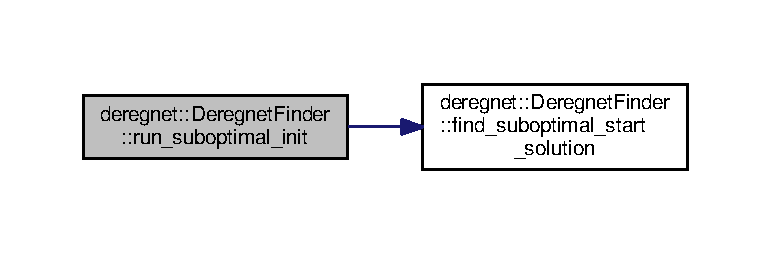
\includegraphics[width=350pt]{classderegnet_1_1DeregnetFinder_ad996cee997a5db4e09016a6f725a6701_cgraph}
\end{center}
\end{figure}
Here is the caller graph for this function\+:\nopagebreak
\begin{figure}[H]
\begin{center}
\leavevmode
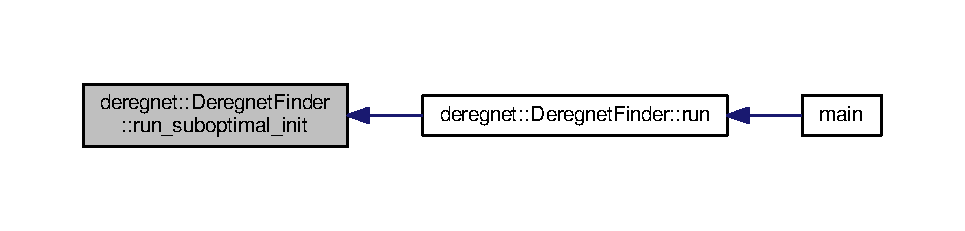
\includegraphics[width=350pt]{classderegnet_1_1DeregnetFinder_ad996cee997a5db4e09016a6f725a6701_icgraph}
\end{center}
\end{figure}
\mbox{\Hypertarget{classderegnet_1_1DeregnetFinder_a4021d92d787877187a24dcbaf0c1bad1}\label{classderegnet_1_1DeregnetFinder_a4021d92d787877187a24dcbaf0c1bad1}} 
\index{deregnet\+::\+Deregnet\+Finder@{deregnet\+::\+Deregnet\+Finder}!run\+\_\+suboptimal\+\_\+windup@{run\+\_\+suboptimal\+\_\+windup}}
\index{run\+\_\+suboptimal\+\_\+windup@{run\+\_\+suboptimal\+\_\+windup}!deregnet\+::\+Deregnet\+Finder@{deregnet\+::\+Deregnet\+Finder}}
\subsubsection{\texorpdfstring{run\+\_\+suboptimal\+\_\+windup()}{run\_suboptimal\_windup()}}
{\footnotesize\ttfamily template$<$typename Model\+Type , typename Data $>$ \\
bool \hyperlink{classderegnet_1_1DeregnetFinder}{deregnet\+::\+Deregnet\+Finder}$<$ Model\+Type, \hyperlink{avgdrgnt_8cpp_a1d1235306db276e9b36acba1db1509e8}{Data} $>$\+::run\+\_\+suboptimal\+\_\+windup (\begin{DoxyParamCaption}\item[{bool}]{solve\+\_\+successful,  }\item[{std\+::vector$<$ \hyperlink{structderegnet_1_1Subgraph}{Subgraph} $>$ $\ast$}]{subgraphs,  }\item[{std\+::set$<$ std\+::string $>$ $\ast$}]{nodes\+\_\+so\+\_\+far,  }\item[{int}]{i }\end{DoxyParamCaption})\hspace{0.3cm}{\ttfamily [private]}}



Post-\/processing after attempt to find suboptimal subgraphs. 



Definition at line 228 of file Deregnet\+Finder.\+hpp.



References deregnet\+::\+Deregnet\+Finder$<$ Model\+Type, Data $>$\+::model, deregnet\+::\+Solution\+::nodes, and deregnet\+::\+Deregnet\+Finder$<$ Model\+Type, Data $>$\+::to\+\_\+subgraph().



Referenced by deregnet\+::\+Deregnet\+Finder$<$ Model\+Type, Data $>$\+::run().


\begin{DoxyCode}
231                                                                    \{
232     \textcolor{comment}{// if a solution was found update subgraphs data structure}
233     \textcolor{comment}{// Also, update the data structure tracking nodes contained in any already found subgraph}
234     \textcolor{keywordflow}{if} ( solve\_successful ) \{
235         Solution current = \hyperlink{classderegnet_1_1DeregnetFinder_ad922d8e38124b4c75daac29a928fcf5b}{model}->getCurrentSolution() ;
236         subgraphs->push\_back(\hyperlink{classderegnet_1_1DeregnetFinder_a681d5e2506f9b6075ab36e742a360328}{to\_subgraph}( current, \textcolor{stringliteral}{"suboptimal\_"} + std::to\_string(i) ));
237         \textcolor{keywordflow}{for} (\textcolor{keyword}{auto} node: current.nodes)
238             nodes\_so\_far->insert(node);
239         \textcolor{keywordflow}{return} \textcolor{keyword}{true};
240     \}
241     \textcolor{comment}{// if no solution was found, issue a message}
242     \textcolor{comment}{// TODO: not necessarily always to std::cout}
243     \textcolor{keywordflow}{else} \{
244         std::cout << \textcolor{stringliteral}{"With these parameters, no more than "} << i
245                   << \textcolor{stringliteral}{" suboptimal subgraphs could be found."} << std::endl;
246         \textcolor{keywordflow}{return} \textcolor{keyword}{false};
247     \}
248 \}
\end{DoxyCode}
Here is the call graph for this function\+:\nopagebreak
\begin{figure}[H]
\begin{center}
\leavevmode
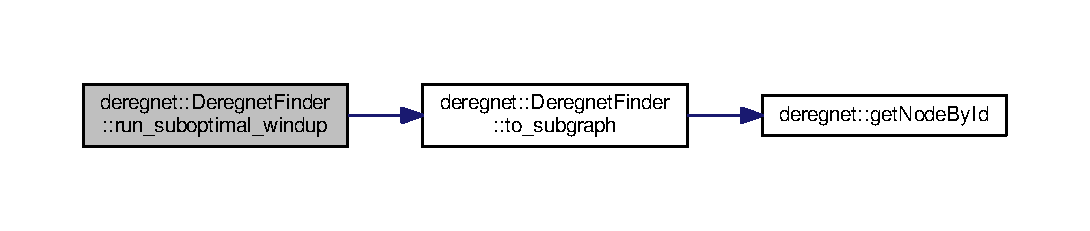
\includegraphics[width=350pt]{classderegnet_1_1DeregnetFinder_a4021d92d787877187a24dcbaf0c1bad1_cgraph}
\end{center}
\end{figure}
Here is the caller graph for this function\+:\nopagebreak
\begin{figure}[H]
\begin{center}
\leavevmode
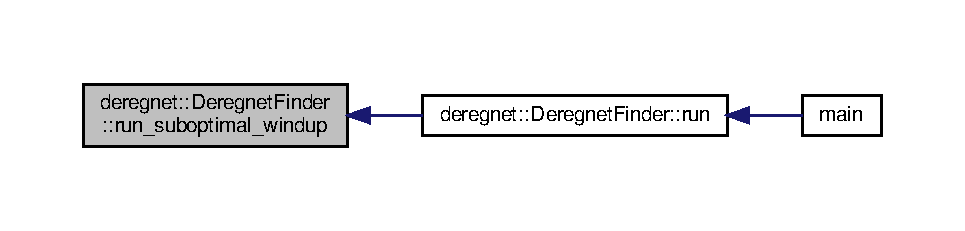
\includegraphics[width=350pt]{classderegnet_1_1DeregnetFinder_a4021d92d787877187a24dcbaf0c1bad1_icgraph}
\end{center}
\end{figure}
\mbox{\Hypertarget{classderegnet_1_1DeregnetFinder_a681d5e2506f9b6075ab36e742a360328}\label{classderegnet_1_1DeregnetFinder_a681d5e2506f9b6075ab36e742a360328}} 
\index{deregnet\+::\+Deregnet\+Finder@{deregnet\+::\+Deregnet\+Finder}!to\+\_\+subgraph@{to\+\_\+subgraph}}
\index{to\+\_\+subgraph@{to\+\_\+subgraph}!deregnet\+::\+Deregnet\+Finder@{deregnet\+::\+Deregnet\+Finder}}
\subsubsection{\texorpdfstring{to\+\_\+subgraph()}{to\_subgraph()}}
{\footnotesize\ttfamily template$<$typename Model\+Type , typename Data $>$ \\
\hyperlink{structderegnet_1_1Subgraph}{Subgraph} \hyperlink{classderegnet_1_1DeregnetFinder}{deregnet\+::\+Deregnet\+Finder}$<$ Model\+Type, \hyperlink{avgdrgnt_8cpp_a1d1235306db276e9b36acba1db1509e8}{Data} $>$\+::to\+\_\+subgraph (\begin{DoxyParamCaption}\item[{\hyperlink{structderegnet_1_1Solution}{Solution}}]{solution,  }\item[{std\+::string}]{signature }\end{DoxyParamCaption})}



Transform a solution from the \hyperlink{structderegnet_1_1Solution}{Solution} type to the \hyperlink{structderegnet_1_1Subgraph}{Subgraph} type. 



Definition at line 280 of file Deregnet\+Finder.\+hpp.



References deregnet\+::\+Solution\+::avg\+\_\+score, deregnet\+::\+Subgraph\+::avg\+\_\+score, deregnet\+::\+Deregnet\+Finder$<$ Model\+Type, Data $>$\+::data, deregnet\+::\+Solution\+::edgelist, deregnet\+::\+Subgraph\+::edgelist, deregnet\+::get\+Node\+By\+Id(), deregnet\+::\+Deregnet\+Data\+::nodeid, deregnet\+::\+Solution\+::nodes, deregnet\+::\+Subgraph\+::nodes, deregnet\+::\+Deregnet\+Data\+::original\+\_\+graph, deregnet\+::\+Deregnet\+Data\+::receptor\+\_\+as\+\_\+root, deregnet\+::\+Deregnet\+Data\+::receptors, deregnet\+::\+Subgraph\+::receptors, deregnet\+::\+Solution\+::rootid, deregnet\+::\+Subgraph\+::rootid, deregnet\+::\+Subgraph\+::signature, deregnet\+::\+Deregnet\+Data\+::terminals, deregnet\+::\+Subgraph\+::terminals, deregnet\+::\+Solution\+::total\+\_\+score, and deregnet\+::\+Subgraph\+::total\+\_\+score.



Referenced by deregnet\+::\+Deregnet\+Finder$<$ Model\+Type, Data $>$\+::run\+\_\+optimal\+\_\+windup(), and deregnet\+::\+Deregnet\+Finder$<$ Model\+Type, Data $>$\+::run\+\_\+suboptimal\+\_\+windup().


\begin{DoxyCode}
280                                                                                             \{
281     Subgraph subgraph;
282     subgraph.signature = signature;
283     subgraph.rootid = solution.rootid;
284     subgraph.nodes = solution.nodes;
285     subgraph.total\_score = solution.total\_score;
286     subgraph.avg\_score = solution.avg\_score;
287     \textcolor{keywordflow}{if} (!\hyperlink{classderegnet_1_1DeregnetFinder_ab158f2a6bb7f39ed3d6e4a9ffe568232}{data}->\hyperlink{classderegnet_1_1DeregnetData_ae7936fe59661a68464134b9251303727}{receptor\_as\_root})
288         swap(\hyperlink{classderegnet_1_1DeregnetFinder_ab158f2a6bb7f39ed3d6e4a9ffe568232}{data}->\hyperlink{classderegnet_1_1DeregnetData_a470cc9f84741c59897ab1e7a3daa1205}{receptors}, \hyperlink{classderegnet_1_1DeregnetFinder_ab158f2a6bb7f39ed3d6e4a9ffe568232}{data}->\hyperlink{classderegnet_1_1DeregnetData_a1fe559c6056cd411647f836849e4b0da}{terminals});
289     \textcolor{keywordflow}{if} (\hyperlink{classderegnet_1_1DeregnetFinder_ab158f2a6bb7f39ed3d6e4a9ffe568232}{data}->\hyperlink{classderegnet_1_1DeregnetData_a470cc9f84741c59897ab1e7a3daa1205}{receptors})
290         \textcolor{keywordflow}{for} (\textcolor{keyword}{auto} nodeid : subgraph.nodes) \{
291             \hyperlink{namespacederegnet_a744bad34f2de9856d36715a445f027f3}{Node} node;
292             \textcolor{keywordflow}{if} (\hyperlink{namespacederegnet_afefc9088a0ea47e8d8c1225b5de29244}{getNodeById}(\hyperlink{classderegnet_1_1DeregnetFinder_ab158f2a6bb7f39ed3d6e4a9ffe568232}{data}->\hyperlink{classderegnet_1_1DeregnetData_a3ea2abe9900785d80fa0141afdd985a9}{original\_graph}, 
      \hyperlink{classderegnet_1_1DeregnetFinder_ab158f2a6bb7f39ed3d6e4a9ffe568232}{data}->\hyperlink{classderegnet_1_1DeregnetData_a3b57d7ed19c104c7fe257e17f0d2cfb5}{nodeid}, nodeid, &node))
293                 \textcolor{keywordflow}{if} (\hyperlink{classderegnet_1_1DeregnetFinder_ab158f2a6bb7f39ed3d6e4a9ffe568232}{data}->\hyperlink{classderegnet_1_1DeregnetData_a470cc9f84741c59897ab1e7a3daa1205}{receptors}->find(node) != \hyperlink{classderegnet_1_1DeregnetFinder_ab158f2a6bb7f39ed3d6e4a9ffe568232}{data}->
      \hyperlink{classderegnet_1_1DeregnetData_a470cc9f84741c59897ab1e7a3daa1205}{receptors}->end())
294                     subgraph.receptors.insert(nodeid);
295         \}
296     \textcolor{keywordflow}{if} (\hyperlink{classderegnet_1_1DeregnetFinder_ab158f2a6bb7f39ed3d6e4a9ffe568232}{data}->\hyperlink{classderegnet_1_1DeregnetData_a1fe559c6056cd411647f836849e4b0da}{terminals})
297         \textcolor{keywordflow}{for} (\textcolor{keyword}{auto} nodeid : subgraph.nodes) \{
298             \hyperlink{namespacederegnet_a744bad34f2de9856d36715a445f027f3}{Node} node;
299             \textcolor{keywordflow}{if} (\hyperlink{namespacederegnet_afefc9088a0ea47e8d8c1225b5de29244}{getNodeById}(\hyperlink{classderegnet_1_1DeregnetFinder_ab158f2a6bb7f39ed3d6e4a9ffe568232}{data}->\hyperlink{classderegnet_1_1DeregnetData_a3ea2abe9900785d80fa0141afdd985a9}{original\_graph}, 
      \hyperlink{classderegnet_1_1DeregnetFinder_ab158f2a6bb7f39ed3d6e4a9ffe568232}{data}->\hyperlink{classderegnet_1_1DeregnetData_a3b57d7ed19c104c7fe257e17f0d2cfb5}{nodeid}, nodeid, &node))
300                 \textcolor{keywordflow}{if} (\hyperlink{classderegnet_1_1DeregnetFinder_ab158f2a6bb7f39ed3d6e4a9ffe568232}{data}->\hyperlink{classderegnet_1_1DeregnetData_a1fe559c6056cd411647f836849e4b0da}{terminals}->find(node) != \hyperlink{classderegnet_1_1DeregnetFinder_ab158f2a6bb7f39ed3d6e4a9ffe568232}{data}->
      \hyperlink{classderegnet_1_1DeregnetData_a1fe559c6056cd411647f836849e4b0da}{terminals}->end())
301                     subgraph.terminals.insert(nodeid);
302         \}
303     \textcolor{keywordflow}{if} (!\hyperlink{classderegnet_1_1DeregnetFinder_ab158f2a6bb7f39ed3d6e4a9ffe568232}{data}->\hyperlink{classderegnet_1_1DeregnetData_ae7936fe59661a68464134b9251303727}{receptor\_as\_root})
304         \textcolor{keywordflow}{for} (\textcolor{keyword}{auto} edge : solution.edgelist)
305             subgraph.edgelist.insert(std::make\_pair(edge.second, edge.first));
306     \textcolor{keywordflow}{else}
307         subgraph.edgelist = solution.edgelist;
308     \textcolor{keywordflow}{return} subgraph;
309 \}
\end{DoxyCode}
Here is the call graph for this function\+:\nopagebreak
\begin{figure}[H]
\begin{center}
\leavevmode
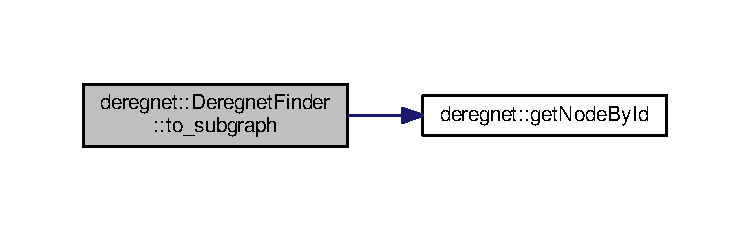
\includegraphics[width=350pt]{classderegnet_1_1DeregnetFinder_a681d5e2506f9b6075ab36e742a360328_cgraph}
\end{center}
\end{figure}
Here is the caller graph for this function\+:\nopagebreak
\begin{figure}[H]
\begin{center}
\leavevmode
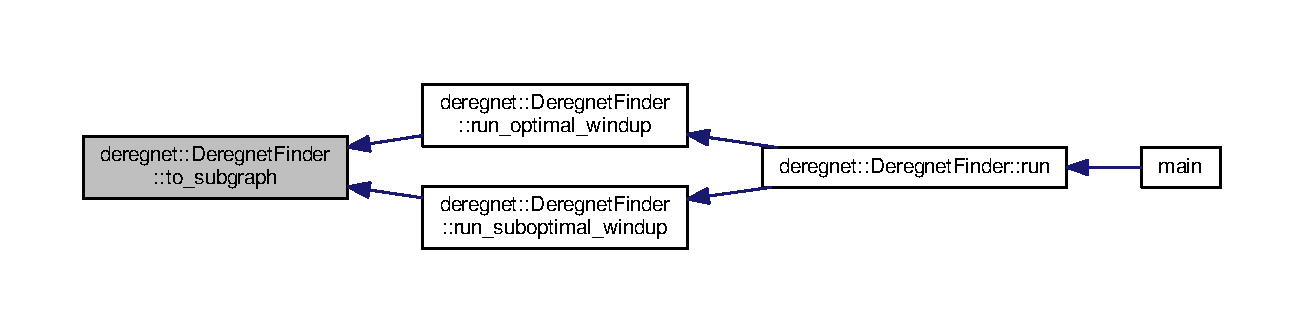
\includegraphics[width=350pt]{classderegnet_1_1DeregnetFinder_a681d5e2506f9b6075ab36e742a360328_icgraph}
\end{center}
\end{figure}


\subsection{Member Data Documentation}
\mbox{\Hypertarget{classderegnet_1_1DeregnetFinder_ab158f2a6bb7f39ed3d6e4a9ffe568232}\label{classderegnet_1_1DeregnetFinder_ab158f2a6bb7f39ed3d6e4a9ffe568232}} 
\index{deregnet\+::\+Deregnet\+Finder@{deregnet\+::\+Deregnet\+Finder}!data@{data}}
\index{data@{data}!deregnet\+::\+Deregnet\+Finder@{deregnet\+::\+Deregnet\+Finder}}
\subsubsection{\texorpdfstring{data}{data}}
{\footnotesize\ttfamily template$<$typename Model\+Type, typename Data$>$ \\
\hyperlink{avgdrgnt_8cpp_a1d1235306db276e9b36acba1db1509e8}{Data}$\ast$ \hyperlink{classderegnet_1_1DeregnetFinder}{deregnet\+::\+Deregnet\+Finder}$<$ Model\+Type, \hyperlink{avgdrgnt_8cpp_a1d1235306db276e9b36acba1db1509e8}{Data} $>$\+::data\hspace{0.3cm}{\ttfamily [private]}}



Pointer to \hyperlink{classderegnet_1_1DeregnetData}{Deregnet\+Data}, i.\+e. \hyperlink{classderegnet_1_1DrgntData}{Drgnt\+Data} or \hyperlink{classderegnet_1_1AvgdrgntData}{Avgdrgnt\+Data}. 



Definition at line 85 of file Deregnet\+Finder.\+hpp.



Referenced by deregnet\+::\+Deregnet\+Finder$<$ Model\+Type, Data $>$\+::find\+\_\+start\+\_\+solution(), deregnet\+::\+Deregnet\+Finder$<$ Model\+Type, Data $>$\+::find\+\_\+suboptimal\+\_\+start\+\_\+solution(), deregnet\+::\+Deregnet\+Finder$<$ Model\+Type, Data $>$\+::run(), deregnet\+::\+Deregnet\+Finder$<$ Model\+Type, Data $>$\+::run\+\_\+optimal\+\_\+init(), deregnet\+::\+Deregnet\+Finder$<$ Model\+Type, Data $>$\+::run\+\_\+suboptimal\+\_\+init(), and deregnet\+::\+Deregnet\+Finder$<$ Model\+Type, Data $>$\+::to\+\_\+subgraph().

\mbox{\Hypertarget{classderegnet_1_1DeregnetFinder_ad922d8e38124b4c75daac29a928fcf5b}\label{classderegnet_1_1DeregnetFinder_ad922d8e38124b4c75daac29a928fcf5b}} 
\index{deregnet\+::\+Deregnet\+Finder@{deregnet\+::\+Deregnet\+Finder}!model@{model}}
\index{model@{model}!deregnet\+::\+Deregnet\+Finder@{deregnet\+::\+Deregnet\+Finder}}
\subsubsection{\texorpdfstring{model}{model}}
{\footnotesize\ttfamily template$<$typename Model\+Type, typename Data$>$ \\
\hyperlink{classderegnet_1_1DeregnetModel}{Deregnet\+Model}$<$Model\+Type, \hyperlink{avgdrgnt_8cpp_a1d1235306db276e9b36acba1db1509e8}{Data}$>$$\ast$ \hyperlink{classderegnet_1_1DeregnetFinder}{deregnet\+::\+Deregnet\+Finder}$<$ Model\+Type, \hyperlink{avgdrgnt_8cpp_a1d1235306db276e9b36acba1db1509e8}{Data} $>$\+::model\hspace{0.3cm}{\ttfamily [private]}}



Model instance to be build and solved. 



Definition at line 86 of file Deregnet\+Finder.\+hpp.



Referenced by deregnet\+::\+Deregnet\+Finder$<$ Model\+Type, Data $>$\+::\+Deregnet\+Finder(), deregnet\+::\+Deregnet\+Finder$<$ Model\+Type, Data $>$\+::run(), deregnet\+::\+Deregnet\+Finder$<$ Model\+Type, Data $>$\+::run\+\_\+optimal\+\_\+init(), deregnet\+::\+Deregnet\+Finder$<$ Model\+Type, Data $>$\+::run\+\_\+optimal\+\_\+windup(), deregnet\+::\+Deregnet\+Finder$<$ Model\+Type, Data $>$\+::run\+\_\+suboptimal\+\_\+init(), and deregnet\+::\+Deregnet\+Finder$<$ Model\+Type, Data $>$\+::run\+\_\+suboptimal\+\_\+windup().



The documentation for this class was generated from the following file\+:\begin{DoxyCompactItemize}
\item 
/datadisk/bbubu/home/self/bbubu/projects/deregnet/src/\hyperlink{DeregnetFinder_8hpp}{Deregnet\+Finder.\+hpp}\end{DoxyCompactItemize}

\hypertarget{classderegnet_1_1DeregnetModel}{}\section{deregnet\+:\+:Deregnet\+Model$<$ Model, Data $>$ Class Template Reference}
\label{classderegnet_1_1DeregnetModel}\index{deregnet\+::\+Deregnet\+Model$<$ Model, Data $>$@{deregnet\+::\+Deregnet\+Model$<$ Model, Data $>$}}


{\ttfamily \#include $<$Deregnet\+Model.\+h$>$}



Collaboration diagram for deregnet\+:\+:Deregnet\+Model$<$ Model, Data $>$\+:\nopagebreak
\begin{figure}[H]
\begin{center}
\leavevmode
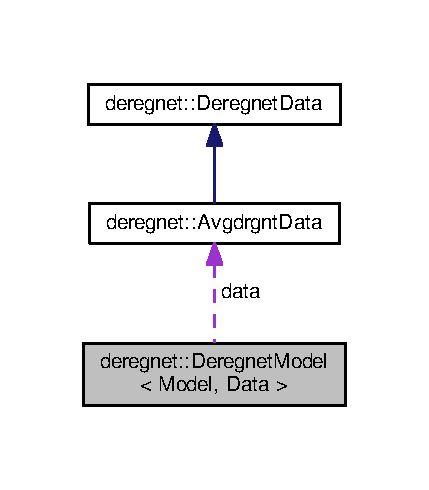
\includegraphics[width=206pt]{classderegnet_1_1DeregnetModel__coll__graph}
\end{center}
\end{figure}
\subsection*{Public Member Functions}
\begin{DoxyCompactItemize}
\item 
\hyperlink{classderegnet_1_1DeregnetModel_a218830114b0bd75965152c5c63a5f4d6}{Deregnet\+Model} (\hyperlink{avgdrgnt_8cpp_a1d1235306db276e9b36acba1db1509e8}{Data} $\ast$\hyperlink{classderegnet_1_1DeregnetModel_ad5399761cf6293a702f3800bda4806d1}{data})
\item 
void \hyperlink{classderegnet_1_1DeregnetModel_ae4dd4e4ae3e796c03d4390eeac1e0a96}{create\+Variables} ()
\item 
void \hyperlink{classderegnet_1_1DeregnetModel_ae246d2286429b83b32e727da987a5817}{add\+Base\+Constraints} ()
\item 
void \hyperlink{classderegnet_1_1DeregnetModel_a6970e42a055fa0dc871d6991ac0feab4}{add\+Include\+Constraints} ()
\item 
void \hyperlink{classderegnet_1_1DeregnetModel_a3b47185dcea73dbcad67d115c55ae762}{add\+Exclude\+Constraints} ()
\item 
void \hyperlink{classderegnet_1_1DeregnetModel_a6d8c05a79c11aefcf05bcdbf9f17aacb}{add\+Receptor\+Constraints} ()
\item 
void \hyperlink{classderegnet_1_1DeregnetModel_aee4a0d40a616c0e6e8787dcca08637aa}{add\+Terminal\+Constraints} ()
\item 
bool \hyperlink{classderegnet_1_1DeregnetModel_af8ca1da09f5a7ebe517fa62249d0b1ab}{solve} (std\+::pair$<$ \hyperlink{namespacederegnet_a744bad34f2de9856d36715a445f027f3}{Node}, std\+::set$<$ \hyperlink{namespacederegnet_a744bad34f2de9856d36715a445f027f3}{Node} $>$$>$ $\ast$start\+\_\+solution)
\item 
void \hyperlink{classderegnet_1_1DeregnetModel_a7cac8e5496b44f04ecf7ff9e450e9a6e}{add\+Suboptimality\+Constraint} (std\+::set$<$ std\+::string $>$ \&nodes\+\_\+so\+\_\+far)
\item 
\hyperlink{structderegnet_1_1Solution}{Solution} \hyperlink{classderegnet_1_1DeregnetModel_a51e1c5476b2425a143908609e75d098a}{get\+Current\+Solution} ()
\item 
{\footnotesize template$<$$>$ }\\void \hyperlink{classderegnet_1_1DeregnetModel_a37d1e4b40f89d3f198196863a8c1d321}{add\+Suboptimality\+Constraint} (std\+::set$<$ std\+::string $>$ \&nodes\+\_\+so\+\_\+far)
\item 
{\footnotesize template$<$$>$ }\\void \hyperlink{classderegnet_1_1DeregnetModel_a266c4a7f90a2884512f98ddcca6750bc}{add\+Suboptimality\+Constraint} (std\+::set$<$ std\+::string $>$ \&nodes\+\_\+so\+\_\+far)
\item 
{\footnotesize template$<$$>$ }\\bool \hyperlink{classderegnet_1_1DeregnetModel_a92c977d9b126c69653401fc45d43879c}{solve} (std\+::pair$<$ \hyperlink{namespacederegnet_a744bad34f2de9856d36715a445f027f3}{Node}, std\+::set$<$ \hyperlink{namespacederegnet_a744bad34f2de9856d36715a445f027f3}{Node} $>$$>$ $\ast$start\+\_\+solution)
\item 
{\footnotesize template$<$$>$ }\\bool \hyperlink{classderegnet_1_1DeregnetModel_a04b8bcc3b59819f10917a6cbb4dea487}{solve} (std\+::pair$<$ \hyperlink{namespacederegnet_a744bad34f2de9856d36715a445f027f3}{Node}, std\+::set$<$ \hyperlink{namespacederegnet_a744bad34f2de9856d36715a445f027f3}{Node} $>$$>$ $\ast$start\+\_\+solution)
\end{DoxyCompactItemize}
\subsection*{Protected Attributes}
\begin{DoxyCompactItemize}
\item 
G\+R\+B\+Env \hyperlink{classderegnet_1_1DeregnetModel_accd03120356b80b083041b4eef003e5b}{env}
\item 
Model \hyperlink{classderegnet_1_1DeregnetModel_a30d525de2086e342b33fe3e45ede4947}{model} \{ Model(\hyperlink{classderegnet_1_1DeregnetModel_accd03120356b80b083041b4eef003e5b}{env}) \}
\item 
std\+::map$<$ \hyperlink{namespacederegnet_a744bad34f2de9856d36715a445f027f3}{Node}, G\+R\+B\+Var $>$ \hyperlink{classderegnet_1_1DeregnetModel_a360c980f3fec4dfbab50e9bb06a933a8}{x}
\item 
std\+::map$<$ \hyperlink{namespacederegnet_a744bad34f2de9856d36715a445f027f3}{Node}, G\+R\+B\+Var $>$ $\ast$ \hyperlink{classderegnet_1_1DeregnetModel_ae76df61afe302b939165facf3dd21ac8}{y} \{ nullptr \}
\item 
\hyperlink{avgdrgnt_8cpp_a1d1235306db276e9b36acba1db1509e8}{Data} $\ast$ \hyperlink{classderegnet_1_1DeregnetModel_ad5399761cf6293a702f3800bda4806d1}{data}
\item 
\hyperlink{namespacederegnet_a55b76c55bbabc682cbc61f8b9948799e}{Graph} $\ast$ \hyperlink{classderegnet_1_1DeregnetModel_a3cd2f54b8e061ef5bed32708d9bc1ef1}{graph}
\item 
\hyperlink{namespacederegnet_ae102b707ae1d6f83c639ece5e0dd5658}{Node\+Map}$<$ double $>$ $\ast$ \hyperlink{classderegnet_1_1DeregnetModel_a46224b0bda5bab796d3b7cb41c184a4d}{score}
\item 
\hyperlink{namespacederegnet_ae102b707ae1d6f83c639ece5e0dd5658}{Node\+Map}$<$ std\+::string $>$ $\ast$ \hyperlink{classderegnet_1_1DeregnetModel_adfebf6f9983c9ccc934469a79381fb78}{nodeid}
\item 
\hyperlink{namespacederegnet_a744bad34f2de9856d36715a445f027f3}{Node} $\ast$ \hyperlink{classderegnet_1_1DeregnetModel_a54b20393a0e26d65935d387685d7fe96}{root}
\end{DoxyCompactItemize}
\subsection*{Private Member Functions}
\begin{DoxyCompactItemize}
\item 
void \hyperlink{classderegnet_1_1DeregnetModel_ad985c03d46183b994dd6f6c037d1c53f}{create\+Variables\+Root} ()
\item 
void \hyperlink{classderegnet_1_1DeregnetModel_ad3700418efd7be24df0d3a16a991a559}{create\+Variables\+No\+Root} ()
\item 
void \hyperlink{classderegnet_1_1DeregnetModel_a65d0e8cac88cc6735659ab41610fd1c9}{add\+Base\+Constraints\+Root} ()
\item 
void \hyperlink{classderegnet_1_1DeregnetModel_a808586dd1edcbadefc04de1c378a6cfa}{add\+Base\+Constraints\+No\+Root} ()
\item 
void \hyperlink{classderegnet_1_1DeregnetModel_a7a76da5bb39123d94c57ba2c940cb1c2}{set\+Start\+Solution} (std\+::pair$<$ \hyperlink{namespacederegnet_a744bad34f2de9856d36715a445f027f3}{Node}, std\+::set$<$ \hyperlink{namespacederegnet_a744bad34f2de9856d36715a445f027f3}{Node} $>$$>$ $\ast$start\+\_\+solution)
\item 
void \hyperlink{classderegnet_1_1DeregnetModel_a502657403c84cbdc66ad845c56dee339}{setup\+\_\+solve} (std\+::pair$<$ \hyperlink{namespacederegnet_a744bad34f2de9856d36715a445f027f3}{Node}, std\+::set$<$ \hyperlink{namespacederegnet_a744bad34f2de9856d36715a445f027f3}{Node} $>$$>$ $\ast$start\+\_\+solution)
\item 
void \hyperlink{classderegnet_1_1DeregnetModel_a19332c492a33a1e488ed916947d38c08}{set\+Callback\+Root} ()
\item 
void \hyperlink{classderegnet_1_1DeregnetModel_a6cecefeafaf782843c91e0c55e768a94}{set\+Callback\+No\+Root} ()
\item 
void \hyperlink{classderegnet_1_1DeregnetModel_a8b4f6be55c874c039c8180c1288f0319}{\+\_\+get\+Current\+Solution} (std\+::string $\ast$rootid, std\+::set$<$ \hyperlink{namespacederegnet_a744bad34f2de9856d36715a445f027f3}{Node} $>$ $\ast$nodes, \hyperlink{structderegnet_1_1Solution}{Solution} $\ast$solution)
\item 
G\+R\+B\+Lin\+Expr \hyperlink{classderegnet_1_1DeregnetModel_ab6093e7558a653c17145e8e08a96938f}{set\+Base\+Constraints\+Root\+Common} ()
\item 
G\+R\+B\+Lin\+Expr \hyperlink{classderegnet_1_1DeregnetModel_a5f6cc627b7a800f3d9d77f5f859d241c}{set\+Base\+Constraints\+No\+Root\+Common} ()
\item 
{\footnotesize template$<$$>$ }\\void \hyperlink{classderegnet_1_1DeregnetModel_a377a4df1d8935fdb5628775df077a029}{add\+Base\+Constraints\+Root} ()
\item 
{\footnotesize template$<$$>$ }\\void \hyperlink{classderegnet_1_1DeregnetModel_ad46d039147e10e7afb08a9ede2fc8a69}{add\+Base\+Constraints\+No\+Root} ()
\item 
{\footnotesize template$<$$>$ }\\void \hyperlink{classderegnet_1_1DeregnetModel_a075dee6e8c4cb899b485dc3627e78791}{add\+Base\+Constraints\+Root} ()
\item 
{\footnotesize template$<$$>$ }\\void \hyperlink{classderegnet_1_1DeregnetModel_a54f3e682bcd27dab4046ac879f69ff91}{add\+Base\+Constraints\+No\+Root} ()
\item 
{\footnotesize template$<$$>$ }\\void \hyperlink{classderegnet_1_1DeregnetModel_aef6cc7f88d0590243d12b9c473ca3ee9}{create\+Variables\+Root} ()
\item 
{\footnotesize template$<$$>$ }\\void \hyperlink{classderegnet_1_1DeregnetModel_a338d7fe9e37a2dc4e4341b10bdce991f}{create\+Variables\+Root} ()
\item 
{\footnotesize template$<$$>$ }\\void \hyperlink{classderegnet_1_1DeregnetModel_aefb0e4b6a3fc7ff0dd6beffc9d826f1d}{create\+Variables\+No\+Root} ()
\item 
{\footnotesize template$<$$>$ }\\void \hyperlink{classderegnet_1_1DeregnetModel_ab0653fa747e69cd61b0721440dc57552}{create\+Variables\+No\+Root} ()
\item 
{\footnotesize template$<$$>$ }\\void \hyperlink{classderegnet_1_1DeregnetModel_afc649e6b52c4e993b17bad158799fdb3}{set\+Start\+Solution} (std\+::pair$<$ \hyperlink{namespacederegnet_a744bad34f2de9856d36715a445f027f3}{Node}, std\+::set$<$ \hyperlink{namespacederegnet_a744bad34f2de9856d36715a445f027f3}{Node} $>$$>$ $\ast$start\+\_\+solution)
\item 
{\footnotesize template$<$$>$ }\\void \hyperlink{classderegnet_1_1DeregnetModel_acb0700e2cc2af475bc99255027e4757a}{set\+Start\+Solution} (std\+::pair$<$ \hyperlink{namespacederegnet_a744bad34f2de9856d36715a445f027f3}{Node}, std\+::set$<$ \hyperlink{namespacederegnet_a744bad34f2de9856d36715a445f027f3}{Node} $>$$>$ $\ast$start\+\_\+solution)
\item 
{\footnotesize template$<$$>$ }\\void \hyperlink{classderegnet_1_1DeregnetModel_a8f10c7fabb80842cd27eb10d31289bbb}{set\+Callback\+Root} ()
\item 
{\footnotesize template$<$$>$ }\\void \hyperlink{classderegnet_1_1DeregnetModel_a1d62ef7fd28d6316d549712bf9214e54}{set\+Callback\+Root} ()
\item 
{\footnotesize template$<$$>$ }\\void \hyperlink{classderegnet_1_1DeregnetModel_a2aacf97af86f2c0f62b9fe4857443400}{set\+Callback\+No\+Root} ()
\item 
{\footnotesize template$<$$>$ }\\void \hyperlink{classderegnet_1_1DeregnetModel_a53356bbd16a9a2bfb51fcdf35da9cc7a}{set\+Callback\+No\+Root} ()
\item 
{\footnotesize template$<$$>$ }\\void \hyperlink{classderegnet_1_1DeregnetModel_ae031344d7bef7965ecbff1af301cc32b}{\+\_\+get\+Current\+Solution} (std\+::string $\ast$rootid, std\+::set$<$ \hyperlink{namespacederegnet_a744bad34f2de9856d36715a445f027f3}{Node} $>$ $\ast$nodes, \hyperlink{structderegnet_1_1Solution}{Solution} $\ast$solution)
\item 
{\footnotesize template$<$$>$ }\\void \hyperlink{classderegnet_1_1DeregnetModel_a38d98fe20d193181c7c5d0655f3c0808}{\+\_\+get\+Current\+Solution} (std\+::string $\ast$rootid, std\+::set$<$ \hyperlink{namespacederegnet_a744bad34f2de9856d36715a445f027f3}{Node} $>$ $\ast$nodes, \hyperlink{structderegnet_1_1Solution}{Solution} $\ast$solution)
\end{DoxyCompactItemize}


\subsection{Detailed Description}
\subsubsection*{template$<$typename Model, typename Data$>$\\*
class deregnet\+::\+Deregnet\+Model$<$ Model, Data $>$}



Definition at line 62 of file Deregnet\+Model.\+h.



\subsection{Constructor \& Destructor Documentation}
\index{deregnet\+::\+Deregnet\+Model@{deregnet\+::\+Deregnet\+Model}!Deregnet\+Model@{Deregnet\+Model}}
\index{Deregnet\+Model@{Deregnet\+Model}!deregnet\+::\+Deregnet\+Model@{deregnet\+::\+Deregnet\+Model}}
\subsubsection[{\texorpdfstring{Deregnet\+Model(\+Data $\ast$data)}{DeregnetModel(Data *data)}}]{\setlength{\rightskip}{0pt plus 5cm}template$<$typename Model , typename Data$>$ {\bf deregnet\+::\+Deregnet\+Model}$<$ Model, {\bf Data} $>$\+::{\bf Deregnet\+Model} (
\begin{DoxyParamCaption}
\item[{{\bf Data} $\ast$}]{data}
\end{DoxyParamCaption}
)}\hypertarget{classderegnet_1_1DeregnetModel_a218830114b0bd75965152c5c63a5f4d6}{}\label{classderegnet_1_1DeregnetModel_a218830114b0bd75965152c5c63a5f4d6}


Definition at line 109 of file Deregnet\+Model.\+h.



References deregnet\+::\+Deregnet\+Model$<$ Model, Data $>$\+::graph, deregnet\+::\+Deregnet\+Model$<$ Model, Data $>$\+::nodeid, deregnet\+::\+Deregnet\+Model$<$ Model, Data $>$\+::root, and deregnet\+::\+Deregnet\+Model$<$ Model, Data $>$\+::score.


\begin{DoxyCode}
110  : data \{ xdata \},
111    \hyperlink{classderegnet_1_1DeregnetModel_a3cd2f54b8e061ef5bed32708d9bc1ef1}{graph} \{ xdata->graph \},
112    \hyperlink{classderegnet_1_1DeregnetModel_a46224b0bda5bab796d3b7cb41c184a4d}{score} \{ xdata->score \},
113    \hyperlink{classderegnet_1_1DeregnetModel_adfebf6f9983c9ccc934469a79381fb78}{nodeid} \{ xdata->nodeid \},
114    \hyperlink{classderegnet_1_1DeregnetModel_a54b20393a0e26d65935d387685d7fe96}{root} \{ xdata->root \}
115 \{ \}
\end{DoxyCode}


\subsection{Member Function Documentation}
\index{deregnet\+::\+Deregnet\+Model@{deregnet\+::\+Deregnet\+Model}!\+\_\+get\+Current\+Solution@{\+\_\+get\+Current\+Solution}}
\index{\+\_\+get\+Current\+Solution@{\+\_\+get\+Current\+Solution}!deregnet\+::\+Deregnet\+Model@{deregnet\+::\+Deregnet\+Model}}
\subsubsection[{\texorpdfstring{\+\_\+get\+Current\+Solution(std\+::string $\ast$rootid, std\+::set$<$ Node $>$ $\ast$nodes, Solution $\ast$solution)}{_getCurrentSolution(std::string *rootid, std::set< Node > *nodes, Solution *solution)}}]{\setlength{\rightskip}{0pt plus 5cm}template$<$typename Model, typename Data$>$ void {\bf deregnet\+::\+Deregnet\+Model}$<$ Model, {\bf Data} $>$\+::\+\_\+get\+Current\+Solution (
\begin{DoxyParamCaption}
\item[{std\+::string $\ast$}]{rootid, }
\item[{std\+::set$<$ {\bf Node} $>$ $\ast$}]{nodes, }
\item[{{\bf Solution} $\ast$}]{solution}
\end{DoxyParamCaption}
)\hspace{0.3cm}{\ttfamily [private]}}\hypertarget{classderegnet_1_1DeregnetModel_a8b4f6be55c874c039c8180c1288f0319}{}\label{classderegnet_1_1DeregnetModel_a8b4f6be55c874c039c8180c1288f0319}


Referenced by deregnet\+::\+Deregnet\+Model$<$ Model, Data $>$\+::get\+Current\+Solution().



Here is the caller graph for this function\+:\nopagebreak
\begin{figure}[H]
\begin{center}
\leavevmode
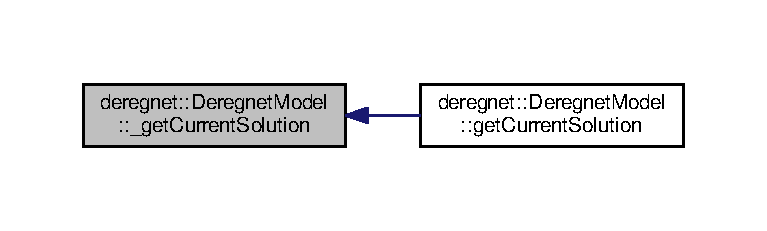
\includegraphics[width=350pt]{classderegnet_1_1DeregnetModel_a8b4f6be55c874c039c8180c1288f0319_icgraph}
\end{center}
\end{figure}


\index{deregnet\+::\+Deregnet\+Model@{deregnet\+::\+Deregnet\+Model}!\+\_\+get\+Current\+Solution@{\+\_\+get\+Current\+Solution}}
\index{\+\_\+get\+Current\+Solution@{\+\_\+get\+Current\+Solution}!deregnet\+::\+Deregnet\+Model@{deregnet\+::\+Deregnet\+Model}}
\subsubsection[{\texorpdfstring{\+\_\+get\+Current\+Solution(std\+::string $\ast$rootid, std\+::set$<$ Node $>$ $\ast$nodes, Solution $\ast$solution)}{_getCurrentSolution(std::string *rootid, std::set< Node > *nodes, Solution *solution)}}]{\setlength{\rightskip}{0pt plus 5cm}template$<$$>$ void {\bf deregnet\+::\+Deregnet\+Model}$<$ G\+R\+B\+Model, {\bf Drgnt\+Data} $>$\+::\+\_\+get\+Current\+Solution (
\begin{DoxyParamCaption}
\item[{std\+::string $\ast$}]{rootid, }
\item[{std\+::set$<$ {\bf Node} $>$ $\ast$}]{nodes, }
\item[{{\bf Solution} $\ast$}]{solution}
\end{DoxyParamCaption}
)\hspace{0.3cm}{\ttfamily [inline]}, {\ttfamily [private]}}\hypertarget{classderegnet_1_1DeregnetModel_ae031344d7bef7965ecbff1af301cc32b}{}\label{classderegnet_1_1DeregnetModel_ae031344d7bef7965ecbff1af301cc32b}


Definition at line 426 of file Deregnet\+Model.\+h.



References deregnet\+::\+Deregnet\+Model$<$ Model, Data $>$\+::graph, I\+N\+V\+A\+L\+ID, deregnet\+::\+Deregnet\+Model$<$ Model, Data $>$\+::model, deregnet\+::\+Deregnet\+Model$<$ Model, Data $>$\+::nodeid, deregnet\+::\+Solution\+::nodes, deregnet\+::\+Deregnet\+Model$<$ Model, Data $>$\+::root, deregnet\+::\+Solution\+::total\+\_\+score, deregnet\+::\+Deregnet\+Model$<$ Model, Data $>$\+::x, and deregnet\+::\+Deregnet\+Model$<$ Model, Data $>$\+::y.


\begin{DoxyCode}
426                                                                                                            
                  \{
427     \textcolor{keywordflow}{for} (\hyperlink{namespacederegnet_ac34314e1b5f456fc6d1bb9d96316de4a}{NodeIt} v(*\hyperlink{classderegnet_1_1DeregnetModel_a3cd2f54b8e061ef5bed32708d9bc1ef1}{graph}); v != \hyperlink{usinglemon_8h_adf770fe2eec438e3758ffe905dbae208}{INVALID}; ++v) \{
428         \textcolor{keywordflow}{if} (\hyperlink{classderegnet_1_1DeregnetModel_a360c980f3fec4dfbab50e9bb06a933a8}{x}[v].\textcolor{keyword}{get}(GRB\_DoubleAttr\_X) >= 0.98) \{
429             nodes->insert(v);
430             (solution->nodes).insert((*\hyperlink{classderegnet_1_1DeregnetModel_adfebf6f9983c9ccc934469a79381fb78}{nodeid})[v]);
431             \textcolor{keywordflow}{if} (!\hyperlink{classderegnet_1_1DeregnetModel_a54b20393a0e26d65935d387685d7fe96}{root}) \{
432                 \textcolor{keywordflow}{if} ((*\hyperlink{classderegnet_1_1DeregnetModel_ae76df61afe302b939165facf3dd21ac8}{y})[v].get(GRB\_DoubleAttr\_X) >= 0.98)
433                     *rootid = (*nodeid)[v];
434             \}
435             \textcolor{keywordflow}{else}
436                 *rootid = (*nodeid)[*\hyperlink{classderegnet_1_1DeregnetModel_a54b20393a0e26d65935d387685d7fe96}{root}];
437         \}
438     \}
439     solution->total\_score = \hyperlink{classderegnet_1_1DeregnetModel_a30d525de2086e342b33fe3e45ede4947}{model}.get(GRB\_DoubleAttr\_ObjVal);
440 \}
\end{DoxyCode}
\index{deregnet\+::\+Deregnet\+Model@{deregnet\+::\+Deregnet\+Model}!\+\_\+get\+Current\+Solution@{\+\_\+get\+Current\+Solution}}
\index{\+\_\+get\+Current\+Solution@{\+\_\+get\+Current\+Solution}!deregnet\+::\+Deregnet\+Model@{deregnet\+::\+Deregnet\+Model}}
\subsubsection[{\texorpdfstring{\+\_\+get\+Current\+Solution(std\+::string $\ast$rootid, std\+::set$<$ Node $>$ $\ast$nodes, Solution $\ast$solution)}{_getCurrentSolution(std::string *rootid, std::set< Node > *nodes, Solution *solution)}}]{\setlength{\rightskip}{0pt plus 5cm}template$<$$>$ void {\bf deregnet\+::\+Deregnet\+Model}$<$ grbfrc\+::\+F\+M\+I\+LP, {\bf Avgdrgnt\+Data} $>$\+::\+\_\+get\+Current\+Solution (
\begin{DoxyParamCaption}
\item[{std\+::string $\ast$}]{rootid, }
\item[{std\+::set$<$ {\bf Node} $>$ $\ast$}]{nodes, }
\item[{{\bf Solution} $\ast$}]{solution}
\end{DoxyParamCaption}
)\hspace{0.3cm}{\ttfamily [inline]}, {\ttfamily [private]}}\hypertarget{classderegnet_1_1DeregnetModel_a38d98fe20d193181c7c5d0655f3c0808}{}\label{classderegnet_1_1DeregnetModel_a38d98fe20d193181c7c5d0655f3c0808}


Definition at line 443 of file Deregnet\+Model.\+h.



References deregnet\+::\+Deregnet\+Model$<$ Model, Data $>$\+::graph, I\+N\+V\+A\+L\+ID, deregnet\+::\+Deregnet\+Model$<$ Model, Data $>$\+::model, deregnet\+::\+Deregnet\+Model$<$ Model, Data $>$\+::nodeid, deregnet\+::\+Solution\+::nodes, deregnet\+::\+Deregnet\+Model$<$ Model, Data $>$\+::root, deregnet\+::\+Solution\+::total\+\_\+score, deregnet\+::\+Deregnet\+Model$<$ Model, Data $>$\+::x, and deregnet\+::\+Deregnet\+Model$<$ Model, Data $>$\+::y.


\begin{DoxyCode}
443                                                                                                            
                        \{
444     \textcolor{keywordflow}{for} (\hyperlink{namespacederegnet_ac34314e1b5f456fc6d1bb9d96316de4a}{NodeIt} v(*\hyperlink{classderegnet_1_1DeregnetModel_a3cd2f54b8e061ef5bed32708d9bc1ef1}{graph}); v != \hyperlink{usinglemon_8h_adf770fe2eec438e3758ffe905dbae208}{INVALID}; ++v) \{
445         \textcolor{keywordflow}{if} (\hyperlink{classderegnet_1_1DeregnetModel_a30d525de2086e342b33fe3e45ede4947}{model}.getVal(\hyperlink{classderegnet_1_1DeregnetModel_a360c980f3fec4dfbab50e9bb06a933a8}{x}[v]) >= 0.98) \{
446             nodes->insert(v);
447             (solution->nodes).insert((*\hyperlink{classderegnet_1_1DeregnetModel_adfebf6f9983c9ccc934469a79381fb78}{nodeid})[v]);
448             \textcolor{keywordflow}{if} (!\hyperlink{classderegnet_1_1DeregnetModel_a54b20393a0e26d65935d387685d7fe96}{root}) \{
449                 \textcolor{keywordflow}{if} (\hyperlink{classderegnet_1_1DeregnetModel_a30d525de2086e342b33fe3e45ede4947}{model}.getVal((*\hyperlink{classderegnet_1_1DeregnetModel_ae76df61afe302b939165facf3dd21ac8}{y})[v]) >= 0.98)
450                     *rootid = (*nodeid)[v];
451             \}
452             \textcolor{keywordflow}{else}
453                 *rootid = (*nodeid)[*\hyperlink{classderegnet_1_1DeregnetModel_a54b20393a0e26d65935d387685d7fe96}{root}];
454         \}
455     \}
456     solution->total\_score = \hyperlink{classderegnet_1_1DeregnetModel_a30d525de2086e342b33fe3e45ede4947}{model}.getObjVal() * nodes->size();
457 \}
\end{DoxyCode}
\index{deregnet\+::\+Deregnet\+Model@{deregnet\+::\+Deregnet\+Model}!add\+Base\+Constraints@{add\+Base\+Constraints}}
\index{add\+Base\+Constraints@{add\+Base\+Constraints}!deregnet\+::\+Deregnet\+Model@{deregnet\+::\+Deregnet\+Model}}
\subsubsection[{\texorpdfstring{add\+Base\+Constraints()}{addBaseConstraints()}}]{\setlength{\rightskip}{0pt plus 5cm}template$<$typename Model , typename Data $>$ void {\bf deregnet\+::\+Deregnet\+Model}$<$ Model, {\bf Data} $>$\+::add\+Base\+Constraints (
\begin{DoxyParamCaption}
{}
\end{DoxyParamCaption}
)}\hypertarget{classderegnet_1_1DeregnetModel_ae246d2286429b83b32e727da987a5817}{}\label{classderegnet_1_1DeregnetModel_ae246d2286429b83b32e727da987a5817}


Definition at line 127 of file Deregnet\+Model.\+h.



References deregnet\+::\+Deregnet\+Model$<$ Model, Data $>$\+::add\+Base\+Constraints\+No\+Root(), deregnet\+::\+Deregnet\+Model$<$ Model, Data $>$\+::add\+Base\+Constraints\+Root(), deregnet\+::\+Deregnet\+Model$<$ Model, Data $>$\+::model, and deregnet\+::\+Deregnet\+Model$<$ Model, Data $>$\+::root.


\begin{DoxyCode}
127                                                     \{
128     \textcolor{keywordflow}{if} (\hyperlink{classderegnet_1_1DeregnetModel_a54b20393a0e26d65935d387685d7fe96}{root})
129         \hyperlink{classderegnet_1_1DeregnetModel_a65d0e8cac88cc6735659ab41610fd1c9}{addBaseConstraintsRoot}();
130     \textcolor{keywordflow}{else}
131         \hyperlink{classderegnet_1_1DeregnetModel_a808586dd1edcbadefc04de1c378a6cfa}{addBaseConstraintsNoRoot}();
132     \hyperlink{classderegnet_1_1DeregnetModel_a30d525de2086e342b33fe3e45ede4947}{model}.update();
133 \}
\end{DoxyCode}


Here is the call graph for this function\+:\nopagebreak
\begin{figure}[H]
\begin{center}
\leavevmode
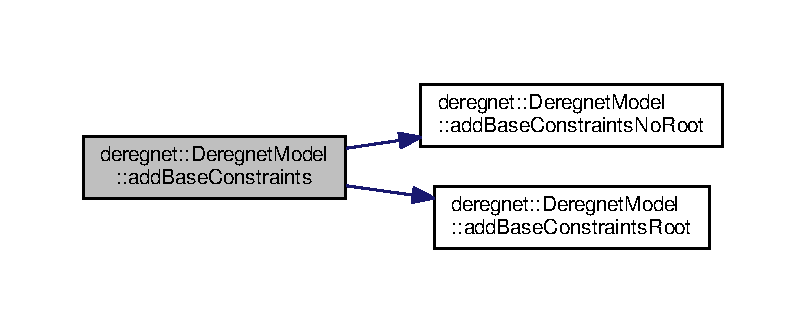
\includegraphics[width=350pt]{classderegnet_1_1DeregnetModel_ae246d2286429b83b32e727da987a5817_cgraph}
\end{center}
\end{figure}


\index{deregnet\+::\+Deregnet\+Model@{deregnet\+::\+Deregnet\+Model}!add\+Base\+Constraints\+No\+Root@{add\+Base\+Constraints\+No\+Root}}
\index{add\+Base\+Constraints\+No\+Root@{add\+Base\+Constraints\+No\+Root}!deregnet\+::\+Deregnet\+Model@{deregnet\+::\+Deregnet\+Model}}
\subsubsection[{\texorpdfstring{add\+Base\+Constraints\+No\+Root()}{addBaseConstraintsNoRoot()}}]{\setlength{\rightskip}{0pt plus 5cm}template$<$typename Model, typename Data$>$ void {\bf deregnet\+::\+Deregnet\+Model}$<$ Model, {\bf Data} $>$\+::add\+Base\+Constraints\+No\+Root (
\begin{DoxyParamCaption}
{}
\end{DoxyParamCaption}
)\hspace{0.3cm}{\ttfamily [private]}}\hypertarget{classderegnet_1_1DeregnetModel_a808586dd1edcbadefc04de1c378a6cfa}{}\label{classderegnet_1_1DeregnetModel_a808586dd1edcbadefc04de1c378a6cfa}


Referenced by deregnet\+::\+Deregnet\+Model$<$ Model, Data $>$\+::add\+Base\+Constraints().



Here is the caller graph for this function\+:\nopagebreak
\begin{figure}[H]
\begin{center}
\leavevmode
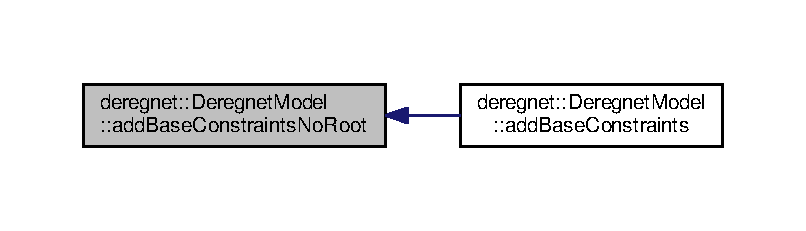
\includegraphics[width=350pt]{classderegnet_1_1DeregnetModel_a808586dd1edcbadefc04de1c378a6cfa_icgraph}
\end{center}
\end{figure}


\index{deregnet\+::\+Deregnet\+Model@{deregnet\+::\+Deregnet\+Model}!add\+Base\+Constraints\+No\+Root@{add\+Base\+Constraints\+No\+Root}}
\index{add\+Base\+Constraints\+No\+Root@{add\+Base\+Constraints\+No\+Root}!deregnet\+::\+Deregnet\+Model@{deregnet\+::\+Deregnet\+Model}}
\subsubsection[{\texorpdfstring{add\+Base\+Constraints\+No\+Root()}{addBaseConstraintsNoRoot()}}]{\setlength{\rightskip}{0pt plus 5cm}template$<$$>$ void {\bf deregnet\+::\+Deregnet\+Model}$<$ G\+R\+B\+Model, {\bf Drgnt\+Data} $>$\+::add\+Base\+Constraints\+No\+Root (
\begin{DoxyParamCaption}
{}
\end{DoxyParamCaption}
)\hspace{0.3cm}{\ttfamily [inline]}, {\ttfamily [private]}}\hypertarget{classderegnet_1_1DeregnetModel_ad46d039147e10e7afb08a9ede2fc8a69}{}\label{classderegnet_1_1DeregnetModel_ad46d039147e10e7afb08a9ede2fc8a69}


Definition at line 174 of file Deregnet\+Model.\+h.



References deregnet\+::\+Deregnet\+Model$<$ Model, Data $>$\+::data, deregnet\+::\+Deregnet\+Model$<$ Model, Data $>$\+::model, and deregnet\+::\+Deregnet\+Model$<$ Model, Data $>$\+::set\+Base\+Constraints\+No\+Root\+Common().


\begin{DoxyCode}
174                                                                   \{
175     GRBLinExpr subgraph\_size\_lhs \{ \hyperlink{classderegnet_1_1DeregnetModel_a5f6cc627b7a800f3d9d77f5f859d241c}{setBaseConstraintsNoRootCommon}() \};
176     \hyperlink{classderegnet_1_1DeregnetModel_a30d525de2086e342b33fe3e45ede4947}{model}.addConstr(subgraph\_size\_lhs == \hyperlink{classderegnet_1_1DeregnetModel_ad5399761cf6293a702f3800bda4806d1}{data}->size);
177 \}
\end{DoxyCode}


Here is the call graph for this function\+:\nopagebreak
\begin{figure}[H]
\begin{center}
\leavevmode
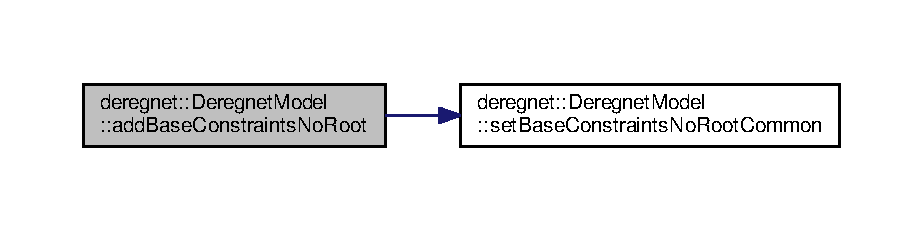
\includegraphics[width=350pt]{classderegnet_1_1DeregnetModel_ad46d039147e10e7afb08a9ede2fc8a69_cgraph}
\end{center}
\end{figure}


\index{deregnet\+::\+Deregnet\+Model@{deregnet\+::\+Deregnet\+Model}!add\+Base\+Constraints\+No\+Root@{add\+Base\+Constraints\+No\+Root}}
\index{add\+Base\+Constraints\+No\+Root@{add\+Base\+Constraints\+No\+Root}!deregnet\+::\+Deregnet\+Model@{deregnet\+::\+Deregnet\+Model}}
\subsubsection[{\texorpdfstring{add\+Base\+Constraints\+No\+Root()}{addBaseConstraintsNoRoot()}}]{\setlength{\rightskip}{0pt plus 5cm}template$<$$>$ void {\bf deregnet\+::\+Deregnet\+Model}$<$ grbfrc\+::\+F\+M\+I\+LP, {\bf Avgdrgnt\+Data} $>$\+::add\+Base\+Constraints\+No\+Root (
\begin{DoxyParamCaption}
{}
\end{DoxyParamCaption}
)\hspace{0.3cm}{\ttfamily [inline]}, {\ttfamily [private]}}\hypertarget{classderegnet_1_1DeregnetModel_a54f3e682bcd27dab4046ac879f69ff91}{}\label{classderegnet_1_1DeregnetModel_a54f3e682bcd27dab4046ac879f69ff91}


Definition at line 187 of file Deregnet\+Model.\+h.



References deregnet\+::\+Deregnet\+Model$<$ Model, Data $>$\+::data, deregnet\+::\+Avgdrgnt\+Data\+::min\+\_\+size, deregnet\+::\+Deregnet\+Model$<$ Model, Data $>$\+::model, and deregnet\+::\+Deregnet\+Model$<$ Model, Data $>$\+::set\+Base\+Constraints\+No\+Root\+Common().


\begin{DoxyCode}
187                                                                         \{
188     GRBLinExpr subgraph\_size\_lhs \{ \hyperlink{classderegnet_1_1DeregnetModel_a5f6cc627b7a800f3d9d77f5f859d241c}{setBaseConstraintsNoRootCommon}() \};
189     \hyperlink{classderegnet_1_1DeregnetModel_a30d525de2086e342b33fe3e45ede4947}{model}.addConstr(\hyperlink{classderegnet_1_1DeregnetModel_ad5399761cf6293a702f3800bda4806d1}{data}->\hyperlink{classderegnet_1_1AvgdrgntData_a733e0cd627433fca043a7f9b70af18c3}{min\_size} <= subgraph\_size\_lhs);
190     \hyperlink{classderegnet_1_1DeregnetModel_a30d525de2086e342b33fe3e45ede4947}{model}.addConstr(subgraph\_size\_lhs <= data->max\_size);
191 \}
\end{DoxyCode}


Here is the call graph for this function\+:\nopagebreak
\begin{figure}[H]
\begin{center}
\leavevmode
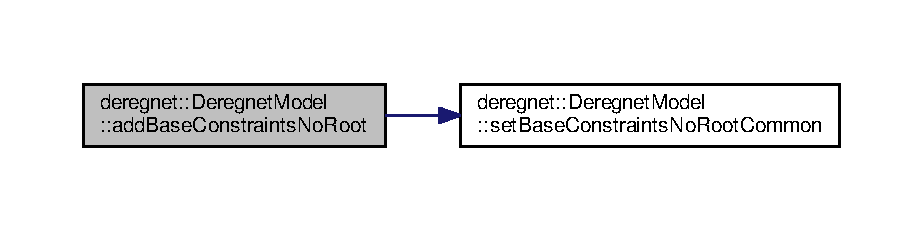
\includegraphics[width=350pt]{classderegnet_1_1DeregnetModel_a54f3e682bcd27dab4046ac879f69ff91_cgraph}
\end{center}
\end{figure}


\index{deregnet\+::\+Deregnet\+Model@{deregnet\+::\+Deregnet\+Model}!add\+Base\+Constraints\+Root@{add\+Base\+Constraints\+Root}}
\index{add\+Base\+Constraints\+Root@{add\+Base\+Constraints\+Root}!deregnet\+::\+Deregnet\+Model@{deregnet\+::\+Deregnet\+Model}}
\subsubsection[{\texorpdfstring{add\+Base\+Constraints\+Root()}{addBaseConstraintsRoot()}}]{\setlength{\rightskip}{0pt plus 5cm}template$<$typename Model, typename Data$>$ void {\bf deregnet\+::\+Deregnet\+Model}$<$ Model, {\bf Data} $>$\+::add\+Base\+Constraints\+Root (
\begin{DoxyParamCaption}
{}
\end{DoxyParamCaption}
)\hspace{0.3cm}{\ttfamily [private]}}\hypertarget{classderegnet_1_1DeregnetModel_a65d0e8cac88cc6735659ab41610fd1c9}{}\label{classderegnet_1_1DeregnetModel_a65d0e8cac88cc6735659ab41610fd1c9}


Referenced by deregnet\+::\+Deregnet\+Model$<$ Model, Data $>$\+::add\+Base\+Constraints().



Here is the caller graph for this function\+:\nopagebreak
\begin{figure}[H]
\begin{center}
\leavevmode
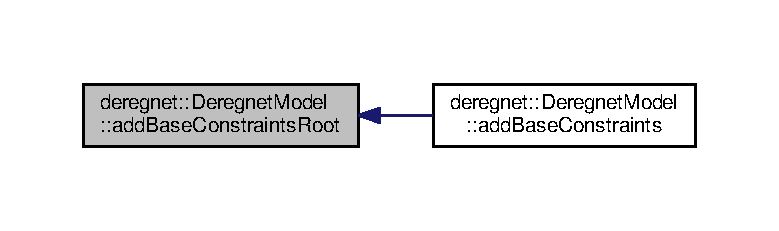
\includegraphics[width=350pt]{classderegnet_1_1DeregnetModel_a65d0e8cac88cc6735659ab41610fd1c9_icgraph}
\end{center}
\end{figure}


\index{deregnet\+::\+Deregnet\+Model@{deregnet\+::\+Deregnet\+Model}!add\+Base\+Constraints\+Root@{add\+Base\+Constraints\+Root}}
\index{add\+Base\+Constraints\+Root@{add\+Base\+Constraints\+Root}!deregnet\+::\+Deregnet\+Model@{deregnet\+::\+Deregnet\+Model}}
\subsubsection[{\texorpdfstring{add\+Base\+Constraints\+Root()}{addBaseConstraintsRoot()}}]{\setlength{\rightskip}{0pt plus 5cm}template$<$$>$ void {\bf deregnet\+::\+Deregnet\+Model}$<$ G\+R\+B\+Model, {\bf Drgnt\+Data} $>$\+::add\+Base\+Constraints\+Root (
\begin{DoxyParamCaption}
{}
\end{DoxyParamCaption}
)\hspace{0.3cm}{\ttfamily [inline]}, {\ttfamily [private]}}\hypertarget{classderegnet_1_1DeregnetModel_a377a4df1d8935fdb5628775df077a029}{}\label{classderegnet_1_1DeregnetModel_a377a4df1d8935fdb5628775df077a029}


Definition at line 168 of file Deregnet\+Model.\+h.



References deregnet\+::\+Deregnet\+Model$<$ Model, Data $>$\+::data, deregnet\+::\+Deregnet\+Model$<$ Model, Data $>$\+::model, and deregnet\+::\+Deregnet\+Model$<$ Model, Data $>$\+::set\+Base\+Constraints\+Root\+Common().


\begin{DoxyCode}
168                                                                 \{
169     GRBLinExpr subgraph\_size\_lhs \{ \hyperlink{classderegnet_1_1DeregnetModel_ab6093e7558a653c17145e8e08a96938f}{setBaseConstraintsRootCommon}() \};
170     \hyperlink{classderegnet_1_1DeregnetModel_a30d525de2086e342b33fe3e45ede4947}{model}.addConstr(subgraph\_size\_lhs == \hyperlink{classderegnet_1_1DeregnetModel_ad5399761cf6293a702f3800bda4806d1}{data}->size);
171 \}
\end{DoxyCode}


Here is the call graph for this function\+:\nopagebreak
\begin{figure}[H]
\begin{center}
\leavevmode
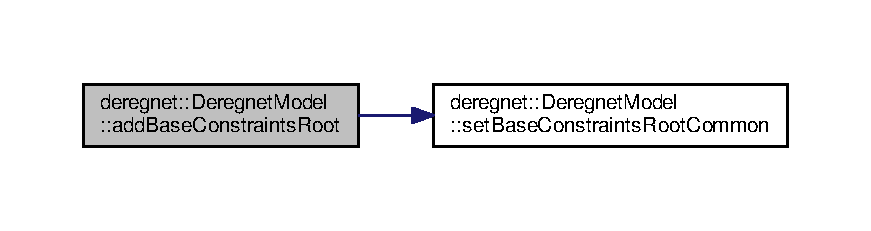
\includegraphics[width=350pt]{classderegnet_1_1DeregnetModel_a377a4df1d8935fdb5628775df077a029_cgraph}
\end{center}
\end{figure}


\index{deregnet\+::\+Deregnet\+Model@{deregnet\+::\+Deregnet\+Model}!add\+Base\+Constraints\+Root@{add\+Base\+Constraints\+Root}}
\index{add\+Base\+Constraints\+Root@{add\+Base\+Constraints\+Root}!deregnet\+::\+Deregnet\+Model@{deregnet\+::\+Deregnet\+Model}}
\subsubsection[{\texorpdfstring{add\+Base\+Constraints\+Root()}{addBaseConstraintsRoot()}}]{\setlength{\rightskip}{0pt plus 5cm}template$<$$>$ void {\bf deregnet\+::\+Deregnet\+Model}$<$ grbfrc\+::\+F\+M\+I\+LP, {\bf Avgdrgnt\+Data} $>$\+::add\+Base\+Constraints\+Root (
\begin{DoxyParamCaption}
{}
\end{DoxyParamCaption}
)\hspace{0.3cm}{\ttfamily [inline]}, {\ttfamily [private]}}\hypertarget{classderegnet_1_1DeregnetModel_a075dee6e8c4cb899b485dc3627e78791}{}\label{classderegnet_1_1DeregnetModel_a075dee6e8c4cb899b485dc3627e78791}


Definition at line 180 of file Deregnet\+Model.\+h.



References deregnet\+::\+Deregnet\+Model$<$ Model, Data $>$\+::data, deregnet\+::\+Avgdrgnt\+Data\+::min\+\_\+size, deregnet\+::\+Deregnet\+Model$<$ Model, Data $>$\+::model, and deregnet\+::\+Deregnet\+Model$<$ Model, Data $>$\+::set\+Base\+Constraints\+Root\+Common().


\begin{DoxyCode}
180                                                                       \{
181     GRBLinExpr subgraph\_size\_lhs \{ \hyperlink{classderegnet_1_1DeregnetModel_ab6093e7558a653c17145e8e08a96938f}{setBaseConstraintsRootCommon}() \};
182     \hyperlink{classderegnet_1_1DeregnetModel_a30d525de2086e342b33fe3e45ede4947}{model}.addConstr(\hyperlink{classderegnet_1_1DeregnetModel_ad5399761cf6293a702f3800bda4806d1}{data}->\hyperlink{classderegnet_1_1AvgdrgntData_a733e0cd627433fca043a7f9b70af18c3}{min\_size} <= subgraph\_size\_lhs);
183     \hyperlink{classderegnet_1_1DeregnetModel_a30d525de2086e342b33fe3e45ede4947}{model}.addConstr(subgraph\_size\_lhs <= data->max\_size);
184 \}
\end{DoxyCode}


Here is the call graph for this function\+:\nopagebreak
\begin{figure}[H]
\begin{center}
\leavevmode
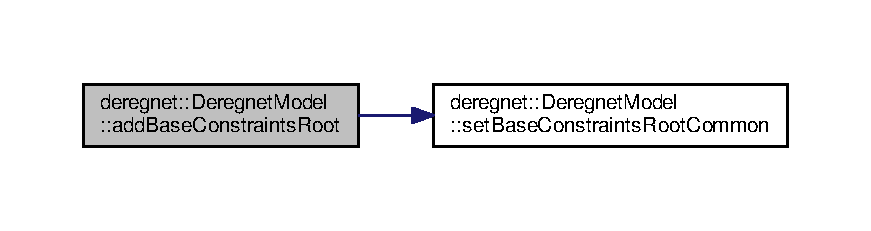
\includegraphics[width=350pt]{classderegnet_1_1DeregnetModel_a075dee6e8c4cb899b485dc3627e78791_cgraph}
\end{center}
\end{figure}


\index{deregnet\+::\+Deregnet\+Model@{deregnet\+::\+Deregnet\+Model}!add\+Exclude\+Constraints@{add\+Exclude\+Constraints}}
\index{add\+Exclude\+Constraints@{add\+Exclude\+Constraints}!deregnet\+::\+Deregnet\+Model@{deregnet\+::\+Deregnet\+Model}}
\subsubsection[{\texorpdfstring{add\+Exclude\+Constraints()}{addExcludeConstraints()}}]{\setlength{\rightskip}{0pt plus 5cm}template$<$typename Model , typename Data $>$ void {\bf deregnet\+::\+Deregnet\+Model}$<$ Model, {\bf Data} $>$\+::add\+Exclude\+Constraints (
\begin{DoxyParamCaption}
{}
\end{DoxyParamCaption}
)}\hypertarget{classderegnet_1_1DeregnetModel_a3b47185dcea73dbcad67d115c55ae762}{}\label{classderegnet_1_1DeregnetModel_a3b47185dcea73dbcad67d115c55ae762}


Definition at line 201 of file Deregnet\+Model.\+h.



References deregnet\+::\+Deregnet\+Model$<$ Model, Data $>$\+::data, deregnet\+::\+Deregnet\+Data\+::exclude, deregnet\+::\+Deregnet\+Model$<$ Model, Data $>$\+::model, and deregnet\+::\+Deregnet\+Model$<$ Model, Data $>$\+::x.


\begin{DoxyCode}
201                                                        \{
202     \textcolor{keywordflow}{for} (\hyperlink{namespacederegnet_a744bad34f2de9856d36715a445f027f3}{Node} v : *(\hyperlink{classderegnet_1_1DeregnetModel_ad5399761cf6293a702f3800bda4806d1}{data}->\hyperlink{classderegnet_1_1DeregnetData_a8e4398e6ece11ef87767914c6f2c304d}{exclude}))
203         \hyperlink{classderegnet_1_1DeregnetModel_a30d525de2086e342b33fe3e45ede4947}{model}.addConstr(\hyperlink{classderegnet_1_1DeregnetModel_a360c980f3fec4dfbab50e9bb06a933a8}{x}[v] == 0);
204     \hyperlink{classderegnet_1_1DeregnetModel_a30d525de2086e342b33fe3e45ede4947}{model}.update();
205 \}
\end{DoxyCode}
\index{deregnet\+::\+Deregnet\+Model@{deregnet\+::\+Deregnet\+Model}!add\+Include\+Constraints@{add\+Include\+Constraints}}
\index{add\+Include\+Constraints@{add\+Include\+Constraints}!deregnet\+::\+Deregnet\+Model@{deregnet\+::\+Deregnet\+Model}}
\subsubsection[{\texorpdfstring{add\+Include\+Constraints()}{addIncludeConstraints()}}]{\setlength{\rightskip}{0pt plus 5cm}template$<$typename Model , typename Data $>$ void {\bf deregnet\+::\+Deregnet\+Model}$<$ Model, {\bf Data} $>$\+::add\+Include\+Constraints (
\begin{DoxyParamCaption}
{}
\end{DoxyParamCaption}
)}\hypertarget{classderegnet_1_1DeregnetModel_a6970e42a055fa0dc871d6991ac0feab4}{}\label{classderegnet_1_1DeregnetModel_a6970e42a055fa0dc871d6991ac0feab4}


Definition at line 194 of file Deregnet\+Model.\+h.



References deregnet\+::\+Deregnet\+Model$<$ Model, Data $>$\+::data, deregnet\+::\+Deregnet\+Data\+::include, deregnet\+::\+Deregnet\+Model$<$ Model, Data $>$\+::model, and deregnet\+::\+Deregnet\+Model$<$ Model, Data $>$\+::x.


\begin{DoxyCode}
194                                                        \{
195     \textcolor{keywordflow}{for} (\hyperlink{namespacederegnet_a744bad34f2de9856d36715a445f027f3}{Node} v : *(\hyperlink{classderegnet_1_1DeregnetModel_ad5399761cf6293a702f3800bda4806d1}{data}->\hyperlink{classderegnet_1_1DeregnetData_a438d16e60be5d119d174aa039f070ab2}{include}))
196         \hyperlink{classderegnet_1_1DeregnetModel_a30d525de2086e342b33fe3e45ede4947}{model}.addConstr(\hyperlink{classderegnet_1_1DeregnetModel_a360c980f3fec4dfbab50e9bb06a933a8}{x}[v] == 1);
197     \hyperlink{classderegnet_1_1DeregnetModel_a30d525de2086e342b33fe3e45ede4947}{model}.update();
198 \}
\end{DoxyCode}
\index{deregnet\+::\+Deregnet\+Model@{deregnet\+::\+Deregnet\+Model}!add\+Receptor\+Constraints@{add\+Receptor\+Constraints}}
\index{add\+Receptor\+Constraints@{add\+Receptor\+Constraints}!deregnet\+::\+Deregnet\+Model@{deregnet\+::\+Deregnet\+Model}}
\subsubsection[{\texorpdfstring{add\+Receptor\+Constraints()}{addReceptorConstraints()}}]{\setlength{\rightskip}{0pt plus 5cm}template$<$typename Model , typename Data $>$ void {\bf deregnet\+::\+Deregnet\+Model}$<$ Model, {\bf Data} $>$\+::add\+Receptor\+Constraints (
\begin{DoxyParamCaption}
{}
\end{DoxyParamCaption}
)}\hypertarget{classderegnet_1_1DeregnetModel_a6d8c05a79c11aefcf05bcdbf9f17aacb}{}\label{classderegnet_1_1DeregnetModel_a6d8c05a79c11aefcf05bcdbf9f17aacb}


Definition at line 208 of file Deregnet\+Model.\+h.



References deregnet\+::\+Deregnet\+Model$<$ Model, Data $>$\+::data, deregnet\+::\+Deregnet\+Model$<$ Model, Data $>$\+::graph, I\+N\+V\+A\+L\+ID, deregnet\+::\+Deregnet\+Model$<$ Model, Data $>$\+::model, deregnet\+::\+Deregnet\+Data\+::receptors, deregnet\+::\+Deregnet\+Model$<$ Model, Data $>$\+::root, and deregnet\+::\+Deregnet\+Model$<$ Model, Data $>$\+::y.


\begin{DoxyCode}
208                                                         \{
209     \textcolor{keywordflow}{if} (!\hyperlink{classderegnet_1_1DeregnetModel_a54b20393a0e26d65935d387685d7fe96}{root}) \{
210         std::set<Node>* receptors \{ \hyperlink{classderegnet_1_1DeregnetModel_ad5399761cf6293a702f3800bda4806d1}{data}->\hyperlink{classderegnet_1_1DeregnetData_a470cc9f84741c59897ab1e7a3daa1205}{receptors} \};
211         \textcolor{keywordflow}{for} (\hyperlink{namespacederegnet_ac34314e1b5f456fc6d1bb9d96316de4a}{NodeIt} v(*\hyperlink{classderegnet_1_1DeregnetModel_a3cd2f54b8e061ef5bed32708d9bc1ef1}{graph}); v != \hyperlink{usinglemon_8h_adf770fe2eec438e3758ffe905dbae208}{INVALID}; ++v)
212             \textcolor{keywordflow}{if} (receptors->find(v) == receptors->end())
213                 \hyperlink{classderegnet_1_1DeregnetModel_a30d525de2086e342b33fe3e45ede4947}{model}.addConstr((*\hyperlink{classderegnet_1_1DeregnetModel_ae76df61afe302b939165facf3dd21ac8}{y})[v] == 0);
214     \}
215     \hyperlink{classderegnet_1_1DeregnetModel_a30d525de2086e342b33fe3e45ede4947}{model}.update();
216 \}
\end{DoxyCode}
\index{deregnet\+::\+Deregnet\+Model@{deregnet\+::\+Deregnet\+Model}!add\+Suboptimality\+Constraint@{add\+Suboptimality\+Constraint}}
\index{add\+Suboptimality\+Constraint@{add\+Suboptimality\+Constraint}!deregnet\+::\+Deregnet\+Model@{deregnet\+::\+Deregnet\+Model}}
\subsubsection[{\texorpdfstring{add\+Suboptimality\+Constraint(std\+::set$<$ std\+::string $>$ \&nodes\+\_\+so\+\_\+far)}{addSuboptimalityConstraint(std::set< std::string > &nodes_so_far)}}]{\setlength{\rightskip}{0pt plus 5cm}template$<$typename Model, typename Data$>$ void {\bf deregnet\+::\+Deregnet\+Model}$<$ Model, {\bf Data} $>$\+::add\+Suboptimality\+Constraint (
\begin{DoxyParamCaption}
\item[{std\+::set$<$ std\+::string $>$ \&}]{nodes\+\_\+so\+\_\+far}
\end{DoxyParamCaption}
)}\hypertarget{classderegnet_1_1DeregnetModel_a7cac8e5496b44f04ecf7ff9e450e9a6e}{}\label{classderegnet_1_1DeregnetModel_a7cac8e5496b44f04ecf7ff9e450e9a6e}
\index{deregnet\+::\+Deregnet\+Model@{deregnet\+::\+Deregnet\+Model}!add\+Suboptimality\+Constraint@{add\+Suboptimality\+Constraint}}
\index{add\+Suboptimality\+Constraint@{add\+Suboptimality\+Constraint}!deregnet\+::\+Deregnet\+Model@{deregnet\+::\+Deregnet\+Model}}
\subsubsection[{\texorpdfstring{add\+Suboptimality\+Constraint(std\+::set$<$ std\+::string $>$ \&nodes\+\_\+so\+\_\+far)}{addSuboptimalityConstraint(std::set< std::string > &nodes_so_far)}}]{\setlength{\rightskip}{0pt plus 5cm}template$<$$>$ void {\bf deregnet\+::\+Deregnet\+Model}$<$ G\+R\+B\+Model, {\bf Drgnt\+Data} $>$\+::add\+Suboptimality\+Constraint (
\begin{DoxyParamCaption}
\item[{std\+::set$<$ std\+::string $>$ \&}]{nodes\+\_\+so\+\_\+far}
\end{DoxyParamCaption}
)\hspace{0.3cm}{\ttfamily [inline]}}\hypertarget{classderegnet_1_1DeregnetModel_a37d1e4b40f89d3f198196863a8c1d321}{}\label{classderegnet_1_1DeregnetModel_a37d1e4b40f89d3f198196863a8c1d321}


Definition at line 308 of file Deregnet\+Model.\+h.



References deregnet\+::\+Deregnet\+Model$<$ Model, Data $>$\+::data, deregnet\+::\+Deregnet\+Model$<$ Model, Data $>$\+::graph, I\+N\+V\+A\+L\+ID, deregnet\+::\+Deregnet\+Model$<$ Model, Data $>$\+::model, deregnet\+::\+Deregnet\+Model$<$ Model, Data $>$\+::nodeid, and deregnet\+::\+Deregnet\+Model$<$ Model, Data $>$\+::x.


\begin{DoxyCode}
308                                                                                                    \{
309     GRBLinExpr nodes\_so\_far\_expr;
310     \textcolor{keywordflow}{for} (\hyperlink{namespacederegnet_ac34314e1b5f456fc6d1bb9d96316de4a}{NodeIt} v(*\hyperlink{classderegnet_1_1DeregnetModel_a3cd2f54b8e061ef5bed32708d9bc1ef1}{graph}); v != \hyperlink{usinglemon_8h_adf770fe2eec438e3758ffe905dbae208}{INVALID}; ++v) \{
311         \textcolor{keywordflow}{if} (nodes\_so\_far.find((*\hyperlink{classderegnet_1_1DeregnetModel_adfebf6f9983c9ccc934469a79381fb78}{nodeid})[v]) != nodes\_so\_far.end())
312             nodes\_so\_far\_expr += \hyperlink{classderegnet_1_1DeregnetModel_a360c980f3fec4dfbab50e9bb06a933a8}{x}[v];
313     \}
314     \hyperlink{classderegnet_1_1DeregnetModel_a30d525de2086e342b33fe3e45ede4947}{model}.addConstr(nodes\_so\_far\_expr <= data->max\_overlap * \hyperlink{classderegnet_1_1DeregnetModel_ad5399761cf6293a702f3800bda4806d1}{data}->size);
315 \}
\end{DoxyCode}
\index{deregnet\+::\+Deregnet\+Model@{deregnet\+::\+Deregnet\+Model}!add\+Suboptimality\+Constraint@{add\+Suboptimality\+Constraint}}
\index{add\+Suboptimality\+Constraint@{add\+Suboptimality\+Constraint}!deregnet\+::\+Deregnet\+Model@{deregnet\+::\+Deregnet\+Model}}
\subsubsection[{\texorpdfstring{add\+Suboptimality\+Constraint(std\+::set$<$ std\+::string $>$ \&nodes\+\_\+so\+\_\+far)}{addSuboptimalityConstraint(std::set< std::string > &nodes_so_far)}}]{\setlength{\rightskip}{0pt plus 5cm}template$<$$>$ void {\bf deregnet\+::\+Deregnet\+Model}$<$ grbfrc\+::\+F\+M\+I\+LP, {\bf Avgdrgnt\+Data} $>$\+::add\+Suboptimality\+Constraint (
\begin{DoxyParamCaption}
\item[{std\+::set$<$ std\+::string $>$ \&}]{nodes\+\_\+so\+\_\+far}
\end{DoxyParamCaption}
)\hspace{0.3cm}{\ttfamily [inline]}}\hypertarget{classderegnet_1_1DeregnetModel_a266c4a7f90a2884512f98ddcca6750bc}{}\label{classderegnet_1_1DeregnetModel_a266c4a7f90a2884512f98ddcca6750bc}


Definition at line 318 of file Deregnet\+Model.\+h.



References deregnet\+::\+Deregnet\+Model$<$ Model, Data $>$\+::graph, I\+N\+V\+A\+L\+ID, deregnet\+::\+Deregnet\+Model$<$ Model, Data $>$\+::model, deregnet\+::\+Deregnet\+Model$<$ Model, Data $>$\+::nodeid, and deregnet\+::\+Deregnet\+Model$<$ Model, Data $>$\+::x.


\begin{DoxyCode}
318                                                                                                          \{
319     GRBLinExpr nodes\_so\_far\_expr;
320     GRBLinExpr size\_expr;
321     \textcolor{keywordflow}{for} (\hyperlink{namespacederegnet_ac34314e1b5f456fc6d1bb9d96316de4a}{NodeIt} v(*\hyperlink{classderegnet_1_1DeregnetModel_a3cd2f54b8e061ef5bed32708d9bc1ef1}{graph}); v != \hyperlink{usinglemon_8h_adf770fe2eec438e3758ffe905dbae208}{INVALID}; ++v) \{
322         size\_expr += \hyperlink{classderegnet_1_1DeregnetModel_a360c980f3fec4dfbab50e9bb06a933a8}{x}[v];
323         \textcolor{keywordflow}{if} (nodes\_so\_far.find((*\hyperlink{classderegnet_1_1DeregnetModel_adfebf6f9983c9ccc934469a79381fb78}{nodeid})[v]) != nodes\_so\_far.end())
324             nodes\_so\_far\_expr += \hyperlink{classderegnet_1_1DeregnetModel_a360c980f3fec4dfbab50e9bb06a933a8}{x}[v];
325     \}
326     \hyperlink{classderegnet_1_1DeregnetModel_a30d525de2086e342b33fe3e45ede4947}{model}.addConstr(nodes\_so\_far\_expr <= data->max\_overlap * size\_expr);
327 \}
\end{DoxyCode}
\index{deregnet\+::\+Deregnet\+Model@{deregnet\+::\+Deregnet\+Model}!add\+Terminal\+Constraints@{add\+Terminal\+Constraints}}
\index{add\+Terminal\+Constraints@{add\+Terminal\+Constraints}!deregnet\+::\+Deregnet\+Model@{deregnet\+::\+Deregnet\+Model}}
\subsubsection[{\texorpdfstring{add\+Terminal\+Constraints()}{addTerminalConstraints()}}]{\setlength{\rightskip}{0pt plus 5cm}template$<$typename Model , typename Data $>$ void {\bf deregnet\+::\+Deregnet\+Model}$<$ Model, {\bf Data} $>$\+::add\+Terminal\+Constraints (
\begin{DoxyParamCaption}
{}
\end{DoxyParamCaption}
)}\hypertarget{classderegnet_1_1DeregnetModel_aee4a0d40a616c0e6e8787dcca08637aa}{}\label{classderegnet_1_1DeregnetModel_aee4a0d40a616c0e6e8787dcca08637aa}


Definition at line 219 of file Deregnet\+Model.\+h.



References deregnet\+::\+Deregnet\+Model$<$ Model, Data $>$\+::data, deregnet\+::\+Deregnet\+Model$<$ Model, Data $>$\+::graph, I\+N\+V\+A\+L\+ID, deregnet\+::\+Deregnet\+Model$<$ Model, Data $>$\+::model, deregnet\+::\+Deregnet\+Data\+::terminals, and deregnet\+::\+Deregnet\+Model$<$ Model, Data $>$\+::x.


\begin{DoxyCode}
219                                                         \{ \textcolor{comment}{// consider using complement of terminals ...}
220     \textcolor{keywordflow}{for} (\hyperlink{namespacederegnet_ac34314e1b5f456fc6d1bb9d96316de4a}{NodeIt} v(*\hyperlink{classderegnet_1_1DeregnetModel_a3cd2f54b8e061ef5bed32708d9bc1ef1}{graph}); v != \hyperlink{usinglemon_8h_adf770fe2eec438e3758ffe905dbae208}{INVALID}; ++v) \{
221         std::set<Node>* terminals \{ \hyperlink{classderegnet_1_1DeregnetModel_ad5399761cf6293a702f3800bda4806d1}{data}->\hyperlink{classderegnet_1_1DeregnetData_a1fe559c6056cd411647f836849e4b0da}{terminals} \};
222         \textcolor{keywordflow}{if} (terminals->find(v) == terminals->end()) \{
223             GRBLinExpr out\_neighbor\_expr;
224             \textcolor{keywordflow}{for} (\hyperlink{namespacederegnet_a253cef939ea250e4cc0c967cd0117853}{OutArcIt} a(*\hyperlink{classderegnet_1_1DeregnetModel_a3cd2f54b8e061ef5bed32708d9bc1ef1}{graph}, v); a != \hyperlink{usinglemon_8h_adf770fe2eec438e3758ffe905dbae208}{INVALID}; ++a)
225                 out\_neighbor\_expr += \hyperlink{classderegnet_1_1DeregnetModel_a360c980f3fec4dfbab50e9bb06a933a8}{x}[\hyperlink{classderegnet_1_1DeregnetModel_a3cd2f54b8e061ef5bed32708d9bc1ef1}{graph}->target(a)];
226             \hyperlink{classderegnet_1_1DeregnetModel_a30d525de2086e342b33fe3e45ede4947}{model}.addConstr(\hyperlink{classderegnet_1_1DeregnetModel_a360c980f3fec4dfbab50e9bb06a933a8}{x}[v] - out\_neighbor\_expr <= 0);
227         \}
228     \}
229     \hyperlink{classderegnet_1_1DeregnetModel_a30d525de2086e342b33fe3e45ede4947}{model}.update();
230 \}
\end{DoxyCode}
\index{deregnet\+::\+Deregnet\+Model@{deregnet\+::\+Deregnet\+Model}!create\+Variables@{create\+Variables}}
\index{create\+Variables@{create\+Variables}!deregnet\+::\+Deregnet\+Model@{deregnet\+::\+Deregnet\+Model}}
\subsubsection[{\texorpdfstring{create\+Variables()}{createVariables()}}]{\setlength{\rightskip}{0pt plus 5cm}template$<$typename Model , typename Data $>$ void {\bf deregnet\+::\+Deregnet\+Model}$<$ Model, {\bf Data} $>$\+::create\+Variables (
\begin{DoxyParamCaption}
{}
\end{DoxyParamCaption}
)}\hypertarget{classderegnet_1_1DeregnetModel_ae4dd4e4ae3e796c03d4390eeac1e0a96}{}\label{classderegnet_1_1DeregnetModel_ae4dd4e4ae3e796c03d4390eeac1e0a96}


Definition at line 118 of file Deregnet\+Model.\+h.



References deregnet\+::\+Deregnet\+Model$<$ Model, Data $>$\+::create\+Variables\+No\+Root(), deregnet\+::\+Deregnet\+Model$<$ Model, Data $>$\+::create\+Variables\+Root(), deregnet\+::\+Deregnet\+Model$<$ Model, Data $>$\+::model, and deregnet\+::\+Deregnet\+Model$<$ Model, Data $>$\+::root.


\begin{DoxyCode}
118                                                  \{
119     \textcolor{keywordflow}{if} (\hyperlink{classderegnet_1_1DeregnetModel_a54b20393a0e26d65935d387685d7fe96}{root})
120         \hyperlink{classderegnet_1_1DeregnetModel_ad985c03d46183b994dd6f6c037d1c53f}{createVariablesRoot}();
121     \textcolor{keywordflow}{else}
122         \hyperlink{classderegnet_1_1DeregnetModel_ad3700418efd7be24df0d3a16a991a559}{createVariablesNoRoot}();
123     \hyperlink{classderegnet_1_1DeregnetModel_a30d525de2086e342b33fe3e45ede4947}{model}.update();
124 \}
\end{DoxyCode}


Here is the call graph for this function\+:\nopagebreak
\begin{figure}[H]
\begin{center}
\leavevmode
\includegraphics[width=350pt]{classderegnet_1_1DeregnetModel_ae4dd4e4ae3e796c03d4390eeac1e0a96_cgraph}
\end{center}
\end{figure}


\index{deregnet\+::\+Deregnet\+Model@{deregnet\+::\+Deregnet\+Model}!create\+Variables\+No\+Root@{create\+Variables\+No\+Root}}
\index{create\+Variables\+No\+Root@{create\+Variables\+No\+Root}!deregnet\+::\+Deregnet\+Model@{deregnet\+::\+Deregnet\+Model}}
\subsubsection[{\texorpdfstring{create\+Variables\+No\+Root()}{createVariablesNoRoot()}}]{\setlength{\rightskip}{0pt plus 5cm}template$<$typename Model, typename Data$>$ void {\bf deregnet\+::\+Deregnet\+Model}$<$ Model, {\bf Data} $>$\+::create\+Variables\+No\+Root (
\begin{DoxyParamCaption}
{}
\end{DoxyParamCaption}
)\hspace{0.3cm}{\ttfamily [private]}}\hypertarget{classderegnet_1_1DeregnetModel_ad3700418efd7be24df0d3a16a991a559}{}\label{classderegnet_1_1DeregnetModel_ad3700418efd7be24df0d3a16a991a559}


Referenced by deregnet\+::\+Deregnet\+Model$<$ Model, Data $>$\+::create\+Variables().



Here is the caller graph for this function\+:\nopagebreak
\begin{figure}[H]
\begin{center}
\leavevmode
\includegraphics[width=350pt]{classderegnet_1_1DeregnetModel_ad3700418efd7be24df0d3a16a991a559_icgraph}
\end{center}
\end{figure}


\index{deregnet\+::\+Deregnet\+Model@{deregnet\+::\+Deregnet\+Model}!create\+Variables\+No\+Root@{create\+Variables\+No\+Root}}
\index{create\+Variables\+No\+Root@{create\+Variables\+No\+Root}!deregnet\+::\+Deregnet\+Model@{deregnet\+::\+Deregnet\+Model}}
\subsubsection[{\texorpdfstring{create\+Variables\+No\+Root()}{createVariablesNoRoot()}}]{\setlength{\rightskip}{0pt plus 5cm}template$<$$>$ void {\bf deregnet\+::\+Deregnet\+Model}$<$ G\+R\+B\+Model, {\bf Drgnt\+Data} $>$\+::create\+Variables\+No\+Root (
\begin{DoxyParamCaption}
{}
\end{DoxyParamCaption}
)\hspace{0.3cm}{\ttfamily [inline]}, {\ttfamily [private]}}\hypertarget{classderegnet_1_1DeregnetModel_aefb0e4b6a3fc7ff0dd6beffc9d826f1d}{}\label{classderegnet_1_1DeregnetModel_aefb0e4b6a3fc7ff0dd6beffc9d826f1d}


Definition at line 290 of file Deregnet\+Model.\+h.



References deregnet\+::\+Deregnet\+Model$<$ Model, Data $>$\+::graph, I\+N\+V\+A\+L\+ID, deregnet\+::\+Deregnet\+Model$<$ Model, Data $>$\+::model, deregnet\+::\+Deregnet\+Model$<$ Model, Data $>$\+::score, deregnet\+::\+Deregnet\+Model$<$ Model, Data $>$\+::x, and deregnet\+::\+Deregnet\+Model$<$ Model, Data $>$\+::y.


\begin{DoxyCode}
290                                                                \{
291     \hyperlink{classderegnet_1_1DeregnetModel_ae76df61afe302b939165facf3dd21ac8}{y} = \textcolor{keyword}{new} std::map<Node, GRBVar>;
292     \textcolor{keywordflow}{for} (\hyperlink{namespacederegnet_ac34314e1b5f456fc6d1bb9d96316de4a}{NodeIt} v(*\hyperlink{classderegnet_1_1DeregnetModel_a3cd2f54b8e061ef5bed32708d9bc1ef1}{graph}); v != \hyperlink{usinglemon_8h_adf770fe2eec438e3758ffe905dbae208}{INVALID}; ++v) \{
293         \hyperlink{classderegnet_1_1DeregnetModel_a360c980f3fec4dfbab50e9bb06a933a8}{x}[v] = \hyperlink{classderegnet_1_1DeregnetModel_a30d525de2086e342b33fe3e45ede4947}{model}.addVar(0.0, 1.0, (*\hyperlink{classderegnet_1_1DeregnetModel_a46224b0bda5bab796d3b7cb41c184a4d}{score})[v], GRB\_BINARY);
294         (*y)[v] = \hyperlink{classderegnet_1_1DeregnetModel_a30d525de2086e342b33fe3e45ede4947}{model}.addVar(0.0, 1.0, 0.0, GRB\_BINARY);
295     \}
296 \}
\end{DoxyCode}
\index{deregnet\+::\+Deregnet\+Model@{deregnet\+::\+Deregnet\+Model}!create\+Variables\+No\+Root@{create\+Variables\+No\+Root}}
\index{create\+Variables\+No\+Root@{create\+Variables\+No\+Root}!deregnet\+::\+Deregnet\+Model@{deregnet\+::\+Deregnet\+Model}}
\subsubsection[{\texorpdfstring{create\+Variables\+No\+Root()}{createVariablesNoRoot()}}]{\setlength{\rightskip}{0pt plus 5cm}template$<$$>$ void {\bf deregnet\+::\+Deregnet\+Model}$<$ grbfrc\+::\+F\+M\+I\+LP, {\bf Avgdrgnt\+Data} $>$\+::create\+Variables\+No\+Root (
\begin{DoxyParamCaption}
{}
\end{DoxyParamCaption}
)\hspace{0.3cm}{\ttfamily [inline]}, {\ttfamily [private]}}\hypertarget{classderegnet_1_1DeregnetModel_ab0653fa747e69cd61b0721440dc57552}{}\label{classderegnet_1_1DeregnetModel_ab0653fa747e69cd61b0721440dc57552}


Definition at line 299 of file Deregnet\+Model.\+h.



References deregnet\+::\+Deregnet\+Model$<$ Model, Data $>$\+::graph, I\+N\+V\+A\+L\+ID, deregnet\+::\+Deregnet\+Model$<$ Model, Data $>$\+::model, deregnet\+::\+Deregnet\+Model$<$ Model, Data $>$\+::score, deregnet\+::\+Deregnet\+Model$<$ Model, Data $>$\+::x, and deregnet\+::\+Deregnet\+Model$<$ Model, Data $>$\+::y.


\begin{DoxyCode}
299                                                                      \{
300     \hyperlink{classderegnet_1_1DeregnetModel_ae76df61afe302b939165facf3dd21ac8}{y} = \textcolor{keyword}{new} std::map<Node, GRBVar>;
301     \textcolor{keywordflow}{for} (\hyperlink{namespacederegnet_ac34314e1b5f456fc6d1bb9d96316de4a}{NodeIt} v(*\hyperlink{classderegnet_1_1DeregnetModel_a3cd2f54b8e061ef5bed32708d9bc1ef1}{graph}); v != \hyperlink{usinglemon_8h_adf770fe2eec438e3758ffe905dbae208}{INVALID}; ++v) \{
302         \hyperlink{classderegnet_1_1DeregnetModel_a360c980f3fec4dfbab50e9bb06a933a8}{x}[v] = \hyperlink{classderegnet_1_1DeregnetModel_a30d525de2086e342b33fe3e45ede4947}{model}.addVar(0.0, 1.0, (*\hyperlink{classderegnet_1_1DeregnetModel_a46224b0bda5bab796d3b7cb41c184a4d}{score})[v], 1.0, GRB\_BINARY);
303         (*y)[v] = \hyperlink{classderegnet_1_1DeregnetModel_a30d525de2086e342b33fe3e45ede4947}{model}.addVar(0.0, 1.0, 0.0, 0.0, GRB\_BINARY);
304     \}
305 \}
\end{DoxyCode}
\index{deregnet\+::\+Deregnet\+Model@{deregnet\+::\+Deregnet\+Model}!create\+Variables\+Root@{create\+Variables\+Root}}
\index{create\+Variables\+Root@{create\+Variables\+Root}!deregnet\+::\+Deregnet\+Model@{deregnet\+::\+Deregnet\+Model}}
\subsubsection[{\texorpdfstring{create\+Variables\+Root()}{createVariablesRoot()}}]{\setlength{\rightskip}{0pt plus 5cm}template$<$typename Model, typename Data$>$ void {\bf deregnet\+::\+Deregnet\+Model}$<$ Model, {\bf Data} $>$\+::create\+Variables\+Root (
\begin{DoxyParamCaption}
{}
\end{DoxyParamCaption}
)\hspace{0.3cm}{\ttfamily [private]}}\hypertarget{classderegnet_1_1DeregnetModel_ad985c03d46183b994dd6f6c037d1c53f}{}\label{classderegnet_1_1DeregnetModel_ad985c03d46183b994dd6f6c037d1c53f}


Referenced by deregnet\+::\+Deregnet\+Model$<$ Model, Data $>$\+::create\+Variables().



Here is the caller graph for this function\+:\nopagebreak
\begin{figure}[H]
\begin{center}
\leavevmode
\includegraphics[width=350pt]{classderegnet_1_1DeregnetModel_ad985c03d46183b994dd6f6c037d1c53f_icgraph}
\end{center}
\end{figure}


\index{deregnet\+::\+Deregnet\+Model@{deregnet\+::\+Deregnet\+Model}!create\+Variables\+Root@{create\+Variables\+Root}}
\index{create\+Variables\+Root@{create\+Variables\+Root}!deregnet\+::\+Deregnet\+Model@{deregnet\+::\+Deregnet\+Model}}
\subsubsection[{\texorpdfstring{create\+Variables\+Root()}{createVariablesRoot()}}]{\setlength{\rightskip}{0pt plus 5cm}template$<$$>$ void {\bf deregnet\+::\+Deregnet\+Model}$<$ G\+R\+B\+Model, {\bf Drgnt\+Data} $>$\+::create\+Variables\+Root (
\begin{DoxyParamCaption}
{}
\end{DoxyParamCaption}
)\hspace{0.3cm}{\ttfamily [inline]}, {\ttfamily [private]}}\hypertarget{classderegnet_1_1DeregnetModel_aef6cc7f88d0590243d12b9c473ca3ee9}{}\label{classderegnet_1_1DeregnetModel_aef6cc7f88d0590243d12b9c473ca3ee9}


Definition at line 278 of file Deregnet\+Model.\+h.



References deregnet\+::\+Deregnet\+Model$<$ Model, Data $>$\+::graph, I\+N\+V\+A\+L\+ID, deregnet\+::\+Deregnet\+Model$<$ Model, Data $>$\+::model, deregnet\+::\+Deregnet\+Model$<$ Model, Data $>$\+::score, and deregnet\+::\+Deregnet\+Model$<$ Model, Data $>$\+::x.


\begin{DoxyCode}
278                                                              \{
279     \textcolor{keywordflow}{for} (\hyperlink{namespacederegnet_ac34314e1b5f456fc6d1bb9d96316de4a}{NodeIt} v(*\hyperlink{classderegnet_1_1DeregnetModel_a3cd2f54b8e061ef5bed32708d9bc1ef1}{graph}); v != \hyperlink{usinglemon_8h_adf770fe2eec438e3758ffe905dbae208}{INVALID}; ++v)
280         \hyperlink{classderegnet_1_1DeregnetModel_a360c980f3fec4dfbab50e9bb06a933a8}{x}[v] = \hyperlink{classderegnet_1_1DeregnetModel_a30d525de2086e342b33fe3e45ede4947}{model}.addVar(0.0, 1.0, (*\hyperlink{classderegnet_1_1DeregnetModel_a46224b0bda5bab796d3b7cb41c184a4d}{score})[v], GRB\_BINARY);
281 \}
\end{DoxyCode}
\index{deregnet\+::\+Deregnet\+Model@{deregnet\+::\+Deregnet\+Model}!create\+Variables\+Root@{create\+Variables\+Root}}
\index{create\+Variables\+Root@{create\+Variables\+Root}!deregnet\+::\+Deregnet\+Model@{deregnet\+::\+Deregnet\+Model}}
\subsubsection[{\texorpdfstring{create\+Variables\+Root()}{createVariablesRoot()}}]{\setlength{\rightskip}{0pt plus 5cm}template$<$$>$ void {\bf deregnet\+::\+Deregnet\+Model}$<$ grbfrc\+::\+F\+M\+I\+LP, {\bf Avgdrgnt\+Data} $>$\+::create\+Variables\+Root (
\begin{DoxyParamCaption}
{}
\end{DoxyParamCaption}
)\hspace{0.3cm}{\ttfamily [inline]}, {\ttfamily [private]}}\hypertarget{classderegnet_1_1DeregnetModel_a338d7fe9e37a2dc4e4341b10bdce991f}{}\label{classderegnet_1_1DeregnetModel_a338d7fe9e37a2dc4e4341b10bdce991f}


Definition at line 284 of file Deregnet\+Model.\+h.



References deregnet\+::\+Deregnet\+Model$<$ Model, Data $>$\+::graph, I\+N\+V\+A\+L\+ID, deregnet\+::\+Deregnet\+Model$<$ Model, Data $>$\+::model, deregnet\+::\+Deregnet\+Model$<$ Model, Data $>$\+::score, and deregnet\+::\+Deregnet\+Model$<$ Model, Data $>$\+::x.


\begin{DoxyCode}
284                                                                    \{
285     \textcolor{keywordflow}{for} (\hyperlink{namespacederegnet_ac34314e1b5f456fc6d1bb9d96316de4a}{NodeIt} v(*\hyperlink{classderegnet_1_1DeregnetModel_a3cd2f54b8e061ef5bed32708d9bc1ef1}{graph}); v != \hyperlink{usinglemon_8h_adf770fe2eec438e3758ffe905dbae208}{INVALID}; ++v)
286         \hyperlink{classderegnet_1_1DeregnetModel_a360c980f3fec4dfbab50e9bb06a933a8}{x}[v] = \hyperlink{classderegnet_1_1DeregnetModel_a30d525de2086e342b33fe3e45ede4947}{model}.addVar(0.0, 1.0, (*\hyperlink{classderegnet_1_1DeregnetModel_a46224b0bda5bab796d3b7cb41c184a4d}{score})[v], 1.0, GRB\_BINARY);
287 \}
\end{DoxyCode}
\index{deregnet\+::\+Deregnet\+Model@{deregnet\+::\+Deregnet\+Model}!get\+Current\+Solution@{get\+Current\+Solution}}
\index{get\+Current\+Solution@{get\+Current\+Solution}!deregnet\+::\+Deregnet\+Model@{deregnet\+::\+Deregnet\+Model}}
\subsubsection[{\texorpdfstring{get\+Current\+Solution()}{getCurrentSolution()}}]{\setlength{\rightskip}{0pt plus 5cm}template$<$typename Model , typename Data $>$ {\bf Solution} {\bf deregnet\+::\+Deregnet\+Model}$<$ Model, {\bf Data} $>$\+::get\+Current\+Solution (
\begin{DoxyParamCaption}
{}
\end{DoxyParamCaption}
)}\hypertarget{classderegnet_1_1DeregnetModel_a51e1c5476b2425a143908609e75d098a}{}\label{classderegnet_1_1DeregnetModel_a51e1c5476b2425a143908609e75d098a}


Definition at line 256 of file Deregnet\+Model.\+h.



References deregnet\+::\+Deregnet\+Model$<$ Model, Data $>$\+::\+\_\+get\+Current\+Solution(), deregnet\+::\+Solution\+::avg\+\_\+score, deregnet\+::\+Solution\+::edgelist, deregnet\+::\+Deregnet\+Model$<$ Model, Data $>$\+::graph, I\+N\+V\+A\+L\+ID, deregnet\+::\+Solution\+::nodes, deregnet\+::\+Solution\+::rootid, and deregnet\+::\+Solution\+::total\+\_\+score.


\begin{DoxyCode}
256                                                         \{
257     Solution solution;
258     std::set<Node> nodes;
259     \textcolor{keywordtype}{string} rootid;
260     \hyperlink{classderegnet_1_1DeregnetModel_a8b4f6be55c874c039c8180c1288f0319}{\_getCurrentSolution}(&rootid, &nodes, &solution);
261     \textcolor{keywordflow}{for} (\textcolor{keyword}{auto} v : nodes) \{
262         std::string source = (*nodeid)[v];
263         \textcolor{keywordflow}{for} (\hyperlink{namespacederegnet_a253cef939ea250e4cc0c967cd0117853}{OutArcIt} a(*\hyperlink{classderegnet_1_1DeregnetModel_a3cd2f54b8e061ef5bed32708d9bc1ef1}{graph}, v); a != \hyperlink{usinglemon_8h_adf770fe2eec438e3758ffe905dbae208}{INVALID}; ++a) \{
264             std::string target \{ (*nodeid)[\hyperlink{classderegnet_1_1DeregnetModel_a3cd2f54b8e061ef5bed32708d9bc1ef1}{graph}->target(a)] \};
265             \textcolor{keywordflow}{if} (solution.nodes.find(target) != solution.nodes.end())
266                 solution.edgelist.insert( std::make\_pair(source, target));
267         \}
268     \}
269     solution.rootid = rootid;
270     solution.avg\_score = solution.total\_score / solution.nodes.size();
271     \textcolor{keywordflow}{return} solution;
272 \}
\end{DoxyCode}


Here is the call graph for this function\+:\nopagebreak
\begin{figure}[H]
\begin{center}
\leavevmode
\includegraphics[width=350pt]{classderegnet_1_1DeregnetModel_a51e1c5476b2425a143908609e75d098a_cgraph}
\end{center}
\end{figure}


\index{deregnet\+::\+Deregnet\+Model@{deregnet\+::\+Deregnet\+Model}!set\+Base\+Constraints\+No\+Root\+Common@{set\+Base\+Constraints\+No\+Root\+Common}}
\index{set\+Base\+Constraints\+No\+Root\+Common@{set\+Base\+Constraints\+No\+Root\+Common}!deregnet\+::\+Deregnet\+Model@{deregnet\+::\+Deregnet\+Model}}
\subsubsection[{\texorpdfstring{set\+Base\+Constraints\+No\+Root\+Common()}{setBaseConstraintsNoRootCommon()}}]{\setlength{\rightskip}{0pt plus 5cm}template$<$typename Model , typename Data $>$ G\+R\+B\+Lin\+Expr {\bf deregnet\+::\+Deregnet\+Model}$<$ Model, {\bf Data} $>$\+::set\+Base\+Constraints\+No\+Root\+Common (
\begin{DoxyParamCaption}
{}
\end{DoxyParamCaption}
)\hspace{0.3cm}{\ttfamily [private]}}\hypertarget{classderegnet_1_1DeregnetModel_a5f6cc627b7a800f3d9d77f5f859d241c}{}\label{classderegnet_1_1DeregnetModel_a5f6cc627b7a800f3d9d77f5f859d241c}


Definition at line 151 of file Deregnet\+Model.\+h.



References deregnet\+::\+Deregnet\+Model$<$ Model, Data $>$\+::graph, I\+N\+V\+A\+L\+ID, deregnet\+::\+Deregnet\+Model$<$ Model, Data $>$\+::model, deregnet\+::\+Deregnet\+Model$<$ Model, Data $>$\+::x, and deregnet\+::\+Deregnet\+Model$<$ Model, Data $>$\+::y.



Referenced by deregnet\+::\+Deregnet\+Model$<$ Model, Data $>$\+::add\+Base\+Constraints\+No\+Root().


\begin{DoxyCode}
151                                                                       \{
152     GRBLinExpr subgraph\_size\_lhs;
153     GRBLinExpr exactly\_one\_root\_lhs;
154     \textcolor{keywordflow}{for} (\hyperlink{namespacederegnet_ac34314e1b5f456fc6d1bb9d96316de4a}{NodeIt} v(*\hyperlink{classderegnet_1_1DeregnetModel_a3cd2f54b8e061ef5bed32708d9bc1ef1}{graph}); v != \hyperlink{usinglemon_8h_adf770fe2eec438e3758ffe905dbae208}{INVALID}; ++v) \{
155         \hyperlink{classderegnet_1_1DeregnetModel_a30d525de2086e342b33fe3e45ede4947}{model}.addConstr((*\hyperlink{classderegnet_1_1DeregnetModel_ae76df61afe302b939165facf3dd21ac8}{y})[v] <= \hyperlink{classderegnet_1_1DeregnetModel_a360c980f3fec4dfbab50e9bb06a933a8}{x}[v]);
156         subgraph\_size\_lhs += \hyperlink{classderegnet_1_1DeregnetModel_a360c980f3fec4dfbab50e9bb06a933a8}{x}[v];
157         exactly\_one\_root\_lhs += (*y)[v];
158         GRBLinExpr parent\_sum;
159         \textcolor{keywordflow}{for} (\hyperlink{namespacederegnet_aed58be361aeda4ef7a9eaca2731ba830}{InArcIt} a(*\hyperlink{classderegnet_1_1DeregnetModel_a3cd2f54b8e061ef5bed32708d9bc1ef1}{graph},v); a != \hyperlink{usinglemon_8h_adf770fe2eec438e3758ffe905dbae208}{INVALID}; ++a)
160             parent\_sum += \hyperlink{classderegnet_1_1DeregnetModel_a360c980f3fec4dfbab50e9bb06a933a8}{x}[\hyperlink{classderegnet_1_1DeregnetModel_a3cd2f54b8e061ef5bed32708d9bc1ef1}{graph}->source(a)];
161         \hyperlink{classderegnet_1_1DeregnetModel_a30d525de2086e342b33fe3e45ede4947}{model}.addConstr(\hyperlink{classderegnet_1_1DeregnetModel_a360c980f3fec4dfbab50e9bb06a933a8}{x}[v] - (*\hyperlink{classderegnet_1_1DeregnetModel_ae76df61afe302b939165facf3dd21ac8}{y})[v] - parent\_sum <= 0);
162     \}
163     \hyperlink{classderegnet_1_1DeregnetModel_a30d525de2086e342b33fe3e45ede4947}{model}.addConstr(exactly\_one\_root\_lhs == 1);
164     \textcolor{keywordflow}{return} subgraph\_size\_lhs;
165 \}
\end{DoxyCode}


Here is the caller graph for this function\+:\nopagebreak
\begin{figure}[H]
\begin{center}
\leavevmode
\includegraphics[width=350pt]{classderegnet_1_1DeregnetModel_a5f6cc627b7a800f3d9d77f5f859d241c_icgraph}
\end{center}
\end{figure}


\index{deregnet\+::\+Deregnet\+Model@{deregnet\+::\+Deregnet\+Model}!set\+Base\+Constraints\+Root\+Common@{set\+Base\+Constraints\+Root\+Common}}
\index{set\+Base\+Constraints\+Root\+Common@{set\+Base\+Constraints\+Root\+Common}!deregnet\+::\+Deregnet\+Model@{deregnet\+::\+Deregnet\+Model}}
\subsubsection[{\texorpdfstring{set\+Base\+Constraints\+Root\+Common()}{setBaseConstraintsRootCommon()}}]{\setlength{\rightskip}{0pt plus 5cm}template$<$typename Model , typename Data $>$ G\+R\+B\+Lin\+Expr {\bf deregnet\+::\+Deregnet\+Model}$<$ Model, {\bf Data} $>$\+::set\+Base\+Constraints\+Root\+Common (
\begin{DoxyParamCaption}
{}
\end{DoxyParamCaption}
)\hspace{0.3cm}{\ttfamily [private]}}\hypertarget{classderegnet_1_1DeregnetModel_ab6093e7558a653c17145e8e08a96938f}{}\label{classderegnet_1_1DeregnetModel_ab6093e7558a653c17145e8e08a96938f}


Definition at line 136 of file Deregnet\+Model.\+h.



References deregnet\+::\+Deregnet\+Model$<$ Model, Data $>$\+::graph, I\+N\+V\+A\+L\+ID, deregnet\+::\+Deregnet\+Model$<$ Model, Data $>$\+::model, deregnet\+::\+Deregnet\+Model$<$ Model, Data $>$\+::root, and deregnet\+::\+Deregnet\+Model$<$ Model, Data $>$\+::x.



Referenced by deregnet\+::\+Deregnet\+Model$<$ Model, Data $>$\+::add\+Base\+Constraints\+Root().


\begin{DoxyCode}
136                                                                     \{
137     GRBLinExpr subgraph\_size\_lhs;
138     \textcolor{keywordflow}{for} (\hyperlink{namespacederegnet_ac34314e1b5f456fc6d1bb9d96316de4a}{NodeIt} v(*\hyperlink{classderegnet_1_1DeregnetModel_a3cd2f54b8e061ef5bed32708d9bc1ef1}{graph}); v != \hyperlink{usinglemon_8h_adf770fe2eec438e3758ffe905dbae208}{INVALID}; ++v) \{
139         subgraph\_size\_lhs += \hyperlink{classderegnet_1_1DeregnetModel_a360c980f3fec4dfbab50e9bb06a933a8}{x}[v];
140         GRBLinExpr parent\_sum;
141         \textcolor{keywordflow}{for} (\hyperlink{namespacederegnet_aed58be361aeda4ef7a9eaca2731ba830}{InArcIt} a(*\hyperlink{classderegnet_1_1DeregnetModel_a3cd2f54b8e061ef5bed32708d9bc1ef1}{graph},v); a != \hyperlink{usinglemon_8h_adf770fe2eec438e3758ffe905dbae208}{INVALID}; ++a)
142             parent\_sum += \hyperlink{classderegnet_1_1DeregnetModel_a360c980f3fec4dfbab50e9bb06a933a8}{x}[\hyperlink{classderegnet_1_1DeregnetModel_a3cd2f54b8e061ef5bed32708d9bc1ef1}{graph}->source(a)];
143         \textcolor{keywordflow}{if} (v != *\hyperlink{classderegnet_1_1DeregnetModel_a54b20393a0e26d65935d387685d7fe96}{root})
144             \hyperlink{classderegnet_1_1DeregnetModel_a30d525de2086e342b33fe3e45ede4947}{model}.addConstr(\hyperlink{classderegnet_1_1DeregnetModel_a360c980f3fec4dfbab50e9bb06a933a8}{x}[v] - parent\_sum <= 0);
145     \}
146     \hyperlink{classderegnet_1_1DeregnetModel_a30d525de2086e342b33fe3e45ede4947}{model}.addConstr(\hyperlink{classderegnet_1_1DeregnetModel_a360c980f3fec4dfbab50e9bb06a933a8}{x}[*\hyperlink{classderegnet_1_1DeregnetModel_a54b20393a0e26d65935d387685d7fe96}{root}] == 1);
147     \textcolor{keywordflow}{return} subgraph\_size\_lhs;
148 \}
\end{DoxyCode}


Here is the caller graph for this function\+:\nopagebreak
\begin{figure}[H]
\begin{center}
\leavevmode
\includegraphics[width=350pt]{classderegnet_1_1DeregnetModel_ab6093e7558a653c17145e8e08a96938f_icgraph}
\end{center}
\end{figure}


\index{deregnet\+::\+Deregnet\+Model@{deregnet\+::\+Deregnet\+Model}!set\+Callback\+No\+Root@{set\+Callback\+No\+Root}}
\index{set\+Callback\+No\+Root@{set\+Callback\+No\+Root}!deregnet\+::\+Deregnet\+Model@{deregnet\+::\+Deregnet\+Model}}
\subsubsection[{\texorpdfstring{set\+Callback\+No\+Root()}{setCallbackNoRoot()}}]{\setlength{\rightskip}{0pt plus 5cm}template$<$typename Model, typename Data$>$ void {\bf deregnet\+::\+Deregnet\+Model}$<$ Model, {\bf Data} $>$\+::set\+Callback\+No\+Root (
\begin{DoxyParamCaption}
{}
\end{DoxyParamCaption}
)\hspace{0.3cm}{\ttfamily [private]}}\hypertarget{classderegnet_1_1DeregnetModel_a6cecefeafaf782843c91e0c55e768a94}{}\label{classderegnet_1_1DeregnetModel_a6cecefeafaf782843c91e0c55e768a94}


Referenced by deregnet\+::\+Deregnet\+Model$<$ Model, Data $>$\+::setup\+\_\+solve().



Here is the caller graph for this function\+:\nopagebreak
\begin{figure}[H]
\begin{center}
\leavevmode
\includegraphics[width=350pt]{classderegnet_1_1DeregnetModel_a6cecefeafaf782843c91e0c55e768a94_icgraph}
\end{center}
\end{figure}


\index{deregnet\+::\+Deregnet\+Model@{deregnet\+::\+Deregnet\+Model}!set\+Callback\+No\+Root@{set\+Callback\+No\+Root}}
\index{set\+Callback\+No\+Root@{set\+Callback\+No\+Root}!deregnet\+::\+Deregnet\+Model@{deregnet\+::\+Deregnet\+Model}}
\subsubsection[{\texorpdfstring{set\+Callback\+No\+Root()}{setCallbackNoRoot()}}]{\setlength{\rightskip}{0pt plus 5cm}template$<$$>$ void {\bf deregnet\+::\+Deregnet\+Model}$<$ G\+R\+B\+Model, {\bf Drgnt\+Data} $>$\+::set\+Callback\+No\+Root (
\begin{DoxyParamCaption}
{}
\end{DoxyParamCaption}
)\hspace{0.3cm}{\ttfamily [inline]}, {\ttfamily [private]}}\hypertarget{classderegnet_1_1DeregnetModel_a2aacf97af86f2c0f62b9fe4857443400}{}\label{classderegnet_1_1DeregnetModel_a2aacf97af86f2c0f62b9fe4857443400}


Definition at line 372 of file Deregnet\+Model.\+h.



References deregnet\+::\+Deregnet\+Model$<$ Model, Data $>$\+::data, deregnet\+::\+Deregnet\+Data\+::gap\+\_\+cut, deregnet\+::\+Deregnet\+Model$<$ Model, Data $>$\+::graph, deregnet\+::\+Deregnet\+Model$<$ Model, Data $>$\+::model, deregnet\+::\+Deregnet\+Model$<$ Model, Data $>$\+::x, and deregnet\+::\+Deregnet\+Model$<$ Model, Data $>$\+::y.


\begin{DoxyCode}
372                                                            \{
373     \hyperlink{classderegnet_1_1DeregnetModel_a30d525de2086e342b33fe3e45ede4947}{model}.setCallback( \textcolor{keyword}{new} LazyConstraintCallbackNoRoot(&\hyperlink{classderegnet_1_1DeregnetModel_a360c980f3fec4dfbab50e9bb06a933a8}{x}, \hyperlink{classderegnet_1_1DeregnetModel_ae76df61afe302b939165facf3dd21ac8}{y}, \hyperlink{classderegnet_1_1DeregnetModel_a3cd2f54b8e061ef5bed32708d9bc1ef1}{graph}, 
      \hyperlink{classderegnet_1_1DeregnetModel_ad5399761cf6293a702f3800bda4806d1}{data}->\hyperlink{classderegnet_1_1DeregnetData_a3637c87366454adc152487fc2f5cfede}{gap\_cut}) );
374 \}
\end{DoxyCode}
\index{deregnet\+::\+Deregnet\+Model@{deregnet\+::\+Deregnet\+Model}!set\+Callback\+No\+Root@{set\+Callback\+No\+Root}}
\index{set\+Callback\+No\+Root@{set\+Callback\+No\+Root}!deregnet\+::\+Deregnet\+Model@{deregnet\+::\+Deregnet\+Model}}
\subsubsection[{\texorpdfstring{set\+Callback\+No\+Root()}{setCallbackNoRoot()}}]{\setlength{\rightskip}{0pt plus 5cm}template$<$$>$ void {\bf deregnet\+::\+Deregnet\+Model}$<$ grbfrc\+::\+F\+M\+I\+LP, {\bf Avgdrgnt\+Data} $>$\+::set\+Callback\+No\+Root (
\begin{DoxyParamCaption}
{}
\end{DoxyParamCaption}
)\hspace{0.3cm}{\ttfamily [inline]}, {\ttfamily [private]}}\hypertarget{classderegnet_1_1DeregnetModel_a53356bbd16a9a2bfb51fcdf35da9cc7a}{}\label{classderegnet_1_1DeregnetModel_a53356bbd16a9a2bfb51fcdf35da9cc7a}


Definition at line 377 of file Deregnet\+Model.\+h.


\begin{DoxyCode}
377                                                                  \{
378 \}
\end{DoxyCode}
\index{deregnet\+::\+Deregnet\+Model@{deregnet\+::\+Deregnet\+Model}!set\+Callback\+Root@{set\+Callback\+Root}}
\index{set\+Callback\+Root@{set\+Callback\+Root}!deregnet\+::\+Deregnet\+Model@{deregnet\+::\+Deregnet\+Model}}
\subsubsection[{\texorpdfstring{set\+Callback\+Root()}{setCallbackRoot()}}]{\setlength{\rightskip}{0pt plus 5cm}template$<$typename Model, typename Data$>$ void {\bf deregnet\+::\+Deregnet\+Model}$<$ Model, {\bf Data} $>$\+::set\+Callback\+Root (
\begin{DoxyParamCaption}
{}
\end{DoxyParamCaption}
)\hspace{0.3cm}{\ttfamily [private]}}\hypertarget{classderegnet_1_1DeregnetModel_a19332c492a33a1e488ed916947d38c08}{}\label{classderegnet_1_1DeregnetModel_a19332c492a33a1e488ed916947d38c08}


Referenced by deregnet\+::\+Deregnet\+Model$<$ Model, Data $>$\+::setup\+\_\+solve().



Here is the caller graph for this function\+:\nopagebreak
\begin{figure}[H]
\begin{center}
\leavevmode
\includegraphics[width=350pt]{classderegnet_1_1DeregnetModel_a19332c492a33a1e488ed916947d38c08_icgraph}
\end{center}
\end{figure}


\index{deregnet\+::\+Deregnet\+Model@{deregnet\+::\+Deregnet\+Model}!set\+Callback\+Root@{set\+Callback\+Root}}
\index{set\+Callback\+Root@{set\+Callback\+Root}!deregnet\+::\+Deregnet\+Model@{deregnet\+::\+Deregnet\+Model}}
\subsubsection[{\texorpdfstring{set\+Callback\+Root()}{setCallbackRoot()}}]{\setlength{\rightskip}{0pt plus 5cm}template$<$$>$ void {\bf deregnet\+::\+Deregnet\+Model}$<$ G\+R\+B\+Model, {\bf Drgnt\+Data} $>$\+::set\+Callback\+Root (
\begin{DoxyParamCaption}
{}
\end{DoxyParamCaption}
)\hspace{0.3cm}{\ttfamily [inline]}, {\ttfamily [private]}}\hypertarget{classderegnet_1_1DeregnetModel_a8f10c7fabb80842cd27eb10d31289bbb}{}\label{classderegnet_1_1DeregnetModel_a8f10c7fabb80842cd27eb10d31289bbb}


Definition at line 363 of file Deregnet\+Model.\+h.



References deregnet\+::\+Deregnet\+Model$<$ Model, Data $>$\+::data, deregnet\+::\+Deregnet\+Data\+::gap\+\_\+cut, deregnet\+::\+Deregnet\+Model$<$ Model, Data $>$\+::graph, deregnet\+::\+Deregnet\+Model$<$ Model, Data $>$\+::model, deregnet\+::\+Deregnet\+Model$<$ Model, Data $>$\+::root, and deregnet\+::\+Deregnet\+Model$<$ Model, Data $>$\+::x.


\begin{DoxyCode}
363                                                          \{
364     \hyperlink{classderegnet_1_1DeregnetModel_a30d525de2086e342b33fe3e45ede4947}{model}.setCallback( \textcolor{keyword}{new} LazyConstraintCallbackRoot(&\hyperlink{classderegnet_1_1DeregnetModel_a360c980f3fec4dfbab50e9bb06a933a8}{x}, \hyperlink{classderegnet_1_1DeregnetModel_a3cd2f54b8e061ef5bed32708d9bc1ef1}{graph}, \hyperlink{classderegnet_1_1DeregnetModel_a54b20393a0e26d65935d387685d7fe96}{root}, 
      \hyperlink{classderegnet_1_1DeregnetModel_ad5399761cf6293a702f3800bda4806d1}{data}->\hyperlink{classderegnet_1_1DeregnetData_a3637c87366454adc152487fc2f5cfede}{gap\_cut}) );
365 \}
\end{DoxyCode}
\index{deregnet\+::\+Deregnet\+Model@{deregnet\+::\+Deregnet\+Model}!set\+Callback\+Root@{set\+Callback\+Root}}
\index{set\+Callback\+Root@{set\+Callback\+Root}!deregnet\+::\+Deregnet\+Model@{deregnet\+::\+Deregnet\+Model}}
\subsubsection[{\texorpdfstring{set\+Callback\+Root()}{setCallbackRoot()}}]{\setlength{\rightskip}{0pt plus 5cm}template$<$$>$ void {\bf deregnet\+::\+Deregnet\+Model}$<$ grbfrc\+::\+F\+M\+I\+LP, {\bf Avgdrgnt\+Data} $>$\+::set\+Callback\+Root (
\begin{DoxyParamCaption}
{}
\end{DoxyParamCaption}
)\hspace{0.3cm}{\ttfamily [inline]}, {\ttfamily [private]}}\hypertarget{classderegnet_1_1DeregnetModel_a1d62ef7fd28d6316d549712bf9214e54}{}\label{classderegnet_1_1DeregnetModel_a1d62ef7fd28d6316d549712bf9214e54}


Definition at line 368 of file Deregnet\+Model.\+h.


\begin{DoxyCode}
368                                                                \{
369 \}
\end{DoxyCode}
\index{deregnet\+::\+Deregnet\+Model@{deregnet\+::\+Deregnet\+Model}!set\+Start\+Solution@{set\+Start\+Solution}}
\index{set\+Start\+Solution@{set\+Start\+Solution}!deregnet\+::\+Deregnet\+Model@{deregnet\+::\+Deregnet\+Model}}
\subsubsection[{\texorpdfstring{set\+Start\+Solution(std\+::pair$<$ Node, std\+::set$<$ Node $>$$>$ $\ast$start\+\_\+solution)}{setStartSolution(std::pair< Node, std::set< Node >> *start_solution)}}]{\setlength{\rightskip}{0pt plus 5cm}template$<$typename Model, typename Data$>$ void {\bf deregnet\+::\+Deregnet\+Model}$<$ Model, {\bf Data} $>$\+::set\+Start\+Solution (
\begin{DoxyParamCaption}
\item[{std\+::pair$<$ {\bf Node}, std\+::set$<$ {\bf Node} $>$$>$ $\ast$}]{start\+\_\+solution}
\end{DoxyParamCaption}
)\hspace{0.3cm}{\ttfamily [private]}}\hypertarget{classderegnet_1_1DeregnetModel_a7a76da5bb39123d94c57ba2c940cb1c2}{}\label{classderegnet_1_1DeregnetModel_a7a76da5bb39123d94c57ba2c940cb1c2}


Referenced by deregnet\+::\+Deregnet\+Model$<$ Model, Data $>$\+::setup\+\_\+solve().



Here is the caller graph for this function\+:\nopagebreak
\begin{figure}[H]
\begin{center}
\leavevmode
\includegraphics[width=350pt]{classderegnet_1_1DeregnetModel_a7a76da5bb39123d94c57ba2c940cb1c2_icgraph}
\end{center}
\end{figure}


\index{deregnet\+::\+Deregnet\+Model@{deregnet\+::\+Deregnet\+Model}!set\+Start\+Solution@{set\+Start\+Solution}}
\index{set\+Start\+Solution@{set\+Start\+Solution}!deregnet\+::\+Deregnet\+Model@{deregnet\+::\+Deregnet\+Model}}
\subsubsection[{\texorpdfstring{set\+Start\+Solution(std\+::pair$<$ Node, std\+::set$<$ Node $>$$>$ $\ast$start\+\_\+solution)}{setStartSolution(std::pair< Node, std::set< Node >> *start_solution)}}]{\setlength{\rightskip}{0pt plus 5cm}template$<$$>$ void {\bf deregnet\+::\+Deregnet\+Model}$<$ G\+R\+B\+Model, {\bf Drgnt\+Data} $>$\+::set\+Start\+Solution (
\begin{DoxyParamCaption}
\item[{std\+::pair$<$ {\bf Node}, std\+::set$<$ {\bf Node} $>$$>$ $\ast$}]{start\+\_\+solution}
\end{DoxyParamCaption}
)\hspace{0.3cm}{\ttfamily [inline]}, {\ttfamily [private]}}\hypertarget{classderegnet_1_1DeregnetModel_afc649e6b52c4e993b17bad158799fdb3}{}\label{classderegnet_1_1DeregnetModel_afc649e6b52c4e993b17bad158799fdb3}


Definition at line 330 of file Deregnet\+Model.\+h.



References deregnet\+::\+Deregnet\+Model$<$ Model, Data $>$\+::graph, I\+N\+V\+A\+L\+ID, deregnet\+::\+Deregnet\+Model$<$ Model, Data $>$\+::root, deregnet\+::\+Deregnet\+Model$<$ Model, Data $>$\+::x, and deregnet\+::\+Deregnet\+Model$<$ Model, Data $>$\+::y.


\begin{DoxyCode}
330                                                                                                      \{
331     \textcolor{keywordflow}{for} (\hyperlink{namespacederegnet_ac34314e1b5f456fc6d1bb9d96316de4a}{NodeIt} v(*\hyperlink{classderegnet_1_1DeregnetModel_a3cd2f54b8e061ef5bed32708d9bc1ef1}{graph}); v != \hyperlink{usinglemon_8h_adf770fe2eec438e3758ffe905dbae208}{INVALID}; ++v) \{
332         \textcolor{keywordflow}{if} ((start\_solution->second).find(v) != (start\_solution->second).end())
333             \hyperlink{classderegnet_1_1DeregnetModel_a360c980f3fec4dfbab50e9bb06a933a8}{x}[v].\textcolor{keyword}{set}(GRB\_DoubleAttr\_Start, 1.0);
334         \textcolor{keywordflow}{else}
335             \hyperlink{classderegnet_1_1DeregnetModel_a360c980f3fec4dfbab50e9bb06a933a8}{x}[v].set(GRB\_DoubleAttr\_Start, 0.0);
336         \textcolor{keywordflow}{if} (!\hyperlink{classderegnet_1_1DeregnetModel_a54b20393a0e26d65935d387685d7fe96}{root}) \{
337             \textcolor{keywordflow}{if} (v == start\_solution->first)
338                 (*y)[v].set(GRB\_DoubleAttr\_Start, 1.0);
339             \textcolor{keywordflow}{else}
340                 (*\hyperlink{classderegnet_1_1DeregnetModel_ae76df61afe302b939165facf3dd21ac8}{y})[v].set(GRB\_DoubleAttr\_Start, 0.0);
341         \}
342     \}
343 \}
\end{DoxyCode}
\index{deregnet\+::\+Deregnet\+Model@{deregnet\+::\+Deregnet\+Model}!set\+Start\+Solution@{set\+Start\+Solution}}
\index{set\+Start\+Solution@{set\+Start\+Solution}!deregnet\+::\+Deregnet\+Model@{deregnet\+::\+Deregnet\+Model}}
\subsubsection[{\texorpdfstring{set\+Start\+Solution(std\+::pair$<$ Node, std\+::set$<$ Node $>$$>$ $\ast$start\+\_\+solution)}{setStartSolution(std::pair< Node, std::set< Node >> *start_solution)}}]{\setlength{\rightskip}{0pt plus 5cm}template$<$$>$ void {\bf deregnet\+::\+Deregnet\+Model}$<$ grbfrc\+::\+F\+M\+I\+LP, {\bf Avgdrgnt\+Data} $>$\+::set\+Start\+Solution (
\begin{DoxyParamCaption}
\item[{std\+::pair$<$ {\bf Node}, std\+::set$<$ {\bf Node} $>$$>$ $\ast$}]{start\+\_\+solution}
\end{DoxyParamCaption}
)\hspace{0.3cm}{\ttfamily [inline]}, {\ttfamily [private]}}\hypertarget{classderegnet_1_1DeregnetModel_acb0700e2cc2af475bc99255027e4757a}{}\label{classderegnet_1_1DeregnetModel_acb0700e2cc2af475bc99255027e4757a}


Definition at line 346 of file Deregnet\+Model.\+h.



References deregnet\+::\+Deregnet\+Model$<$ Model, Data $>$\+::graph, I\+N\+V\+A\+L\+ID, deregnet\+::\+Deregnet\+Model$<$ Model, Data $>$\+::model, deregnet\+::\+Deregnet\+Model$<$ Model, Data $>$\+::root, deregnet\+::\+Deregnet\+Model$<$ Model, Data $>$\+::x, and deregnet\+::\+Deregnet\+Model$<$ Model, Data $>$\+::y.


\begin{DoxyCode}
346                                                                                                            
      \{
347     \textcolor{keywordflow}{for} (\hyperlink{namespacederegnet_ac34314e1b5f456fc6d1bb9d96316de4a}{NodeIt} v(*\hyperlink{classderegnet_1_1DeregnetModel_a3cd2f54b8e061ef5bed32708d9bc1ef1}{graph}); v != \hyperlink{usinglemon_8h_adf770fe2eec438e3758ffe905dbae208}{INVALID}; ++v) \{
348         \textcolor{keywordflow}{if} ((start\_solution->second).find(v) != (start\_solution->second).end())
349             \hyperlink{classderegnet_1_1DeregnetModel_a30d525de2086e342b33fe3e45ede4947}{model}.setStartSolution(\hyperlink{classderegnet_1_1DeregnetModel_a360c980f3fec4dfbab50e9bb06a933a8}{x}[v], 1.0);
350         \textcolor{keywordflow}{else}
351             \hyperlink{classderegnet_1_1DeregnetModel_a30d525de2086e342b33fe3e45ede4947}{model}.setStartSolution(\hyperlink{classderegnet_1_1DeregnetModel_a360c980f3fec4dfbab50e9bb06a933a8}{x}[v], 1.0);
352         \textcolor{keywordflow}{if} (!\hyperlink{classderegnet_1_1DeregnetModel_a54b20393a0e26d65935d387685d7fe96}{root}) \{
353             \textcolor{keywordflow}{if} (v == start\_solution->first)
354                 \hyperlink{classderegnet_1_1DeregnetModel_a30d525de2086e342b33fe3e45ede4947}{model}.setStartSolution((*\hyperlink{classderegnet_1_1DeregnetModel_ae76df61afe302b939165facf3dd21ac8}{y})[v], 1.0);
355             \textcolor{keywordflow}{else}
356                 \hyperlink{classderegnet_1_1DeregnetModel_a30d525de2086e342b33fe3e45ede4947}{model}.setStartSolution((*\hyperlink{classderegnet_1_1DeregnetModel_ae76df61afe302b939165facf3dd21ac8}{y})[v], 0.0);
357         \}
358     \}
359 \}
\end{DoxyCode}
\index{deregnet\+::\+Deregnet\+Model@{deregnet\+::\+Deregnet\+Model}!setup\+\_\+solve@{setup\+\_\+solve}}
\index{setup\+\_\+solve@{setup\+\_\+solve}!deregnet\+::\+Deregnet\+Model@{deregnet\+::\+Deregnet\+Model}}
\subsubsection[{\texorpdfstring{setup\+\_\+solve(std\+::pair$<$ Node, std\+::set$<$ Node $>$$>$ $\ast$start\+\_\+solution)}{setup_solve(std::pair< Node, std::set< Node >> *start_solution)}}]{\setlength{\rightskip}{0pt plus 5cm}template$<$typename Model , typename Data $>$ void {\bf deregnet\+::\+Deregnet\+Model}$<$ Model, {\bf Data} $>$\+::setup\+\_\+solve (
\begin{DoxyParamCaption}
\item[{std\+::pair$<$ {\bf Node}, std\+::set$<$ {\bf Node} $>$$>$ $\ast$}]{start\+\_\+solution}
\end{DoxyParamCaption}
)\hspace{0.3cm}{\ttfamily [private]}}\hypertarget{classderegnet_1_1DeregnetModel_a502657403c84cbdc66ad845c56dee339}{}\label{classderegnet_1_1DeregnetModel_a502657403c84cbdc66ad845c56dee339}


Definition at line 233 of file Deregnet\+Model.\+h.



References deregnet\+::\+Deregnet\+Model$<$ Model, Data $>$\+::data, deregnet\+::\+Deregnet\+Model$<$ Model, Data $>$\+::model, deregnet\+::\+Deregnet\+Data\+::model\+\_\+sense, deregnet\+::\+Deregnet\+Model$<$ Model, Data $>$\+::root, deregnet\+::\+Deregnet\+Model$<$ Model, Data $>$\+::set\+Callback\+No\+Root(), deregnet\+::\+Deregnet\+Model$<$ Model, Data $>$\+::set\+Callback\+Root(), deregnet\+::\+Deregnet\+Model$<$ Model, Data $>$\+::set\+Start\+Solution(), and deregnet\+::\+Deregnet\+Data\+::time\+\_\+limit.



Referenced by deregnet\+::\+Deregnet\+Model$<$ Model, Data $>$\+::solve().


\begin{DoxyCode}
233                                                                                         \{
234     \textcolor{keywordflow}{if} (\hyperlink{classderegnet_1_1DeregnetModel_ad5399761cf6293a702f3800bda4806d1}{data}->\hyperlink{classderegnet_1_1DeregnetData_ac3918536b5423facf0ac155997703c52}{model\_sense} == \textcolor{stringliteral}{"min"})
235         \hyperlink{classderegnet_1_1DeregnetModel_a30d525de2086e342b33fe3e45ede4947}{model}.set(GRB\_IntAttr\_ModelSense, GRB\_MINIMIZE);
236     \textcolor{keywordflow}{else}
237         \hyperlink{classderegnet_1_1DeregnetModel_a30d525de2086e342b33fe3e45ede4947}{model}.set(GRB\_IntAttr\_ModelSense, GRB\_MAXIMIZE);
238 
239     \hyperlink{classderegnet_1_1DeregnetModel_a30d525de2086e342b33fe3e45ede4947}{model}.set(GRB\_IntParam\_LazyConstraints, 1);
240 
241     \textcolor{keywordflow}{if} (\hyperlink{classderegnet_1_1DeregnetModel_ad5399761cf6293a702f3800bda4806d1}{data}->\hyperlink{classderegnet_1_1DeregnetData_ac378faf7e8466135b8dc0ced907d98ae}{time\_limit})
242         \hyperlink{classderegnet_1_1DeregnetModel_a30d525de2086e342b33fe3e45ede4947}{model}.set(GRB\_DoubleParam\_TimeLimit, *(\hyperlink{classderegnet_1_1DeregnetModel_ad5399761cf6293a702f3800bda4806d1}{data}->\hyperlink{classderegnet_1_1DeregnetData_ac378faf7e8466135b8dc0ced907d98ae}{time\_limit}));
243 
244     \textcolor{keywordflow}{if} (start\_solution)
245         \hyperlink{classderegnet_1_1DeregnetModel_a7a76da5bb39123d94c57ba2c940cb1c2}{setStartSolution}(start\_solution);
246 
247     \textcolor{keywordflow}{if} (\hyperlink{classderegnet_1_1DeregnetModel_a54b20393a0e26d65935d387685d7fe96}{root})
248         \hyperlink{classderegnet_1_1DeregnetModel_a19332c492a33a1e488ed916947d38c08}{setCallbackRoot}();
249     \textcolor{keywordflow}{else}
250         \hyperlink{classderegnet_1_1DeregnetModel_a6cecefeafaf782843c91e0c55e768a94}{setCallbackNoRoot}();
251     \hyperlink{classderegnet_1_1DeregnetModel_a30d525de2086e342b33fe3e45ede4947}{model}.update();
252 \}
\end{DoxyCode}


Here is the call graph for this function\+:\nopagebreak
\begin{figure}[H]
\begin{center}
\leavevmode
\includegraphics[width=350pt]{classderegnet_1_1DeregnetModel_a502657403c84cbdc66ad845c56dee339_cgraph}
\end{center}
\end{figure}




Here is the caller graph for this function\+:\nopagebreak
\begin{figure}[H]
\begin{center}
\leavevmode
\includegraphics[width=350pt]{classderegnet_1_1DeregnetModel_a502657403c84cbdc66ad845c56dee339_icgraph}
\end{center}
\end{figure}


\index{deregnet\+::\+Deregnet\+Model@{deregnet\+::\+Deregnet\+Model}!solve@{solve}}
\index{solve@{solve}!deregnet\+::\+Deregnet\+Model@{deregnet\+::\+Deregnet\+Model}}
\subsubsection[{\texorpdfstring{solve(std\+::pair$<$ Node, std\+::set$<$ Node $>$$>$ $\ast$start\+\_\+solution)}{solve(std::pair< Node, std::set< Node >> *start_solution)}}]{\setlength{\rightskip}{0pt plus 5cm}template$<$typename Model, typename Data$>$ bool {\bf deregnet\+::\+Deregnet\+Model}$<$ Model, {\bf Data} $>$\+::solve (
\begin{DoxyParamCaption}
\item[{std\+::pair$<$ {\bf Node}, std\+::set$<$ {\bf Node} $>$$>$ $\ast$}]{start\+\_\+solution}
\end{DoxyParamCaption}
)}\hypertarget{classderegnet_1_1DeregnetModel_af8ca1da09f5a7ebe517fa62249d0b1ab}{}\label{classderegnet_1_1DeregnetModel_af8ca1da09f5a7ebe517fa62249d0b1ab}
\index{deregnet\+::\+Deregnet\+Model@{deregnet\+::\+Deregnet\+Model}!solve@{solve}}
\index{solve@{solve}!deregnet\+::\+Deregnet\+Model@{deregnet\+::\+Deregnet\+Model}}
\subsubsection[{\texorpdfstring{solve(std\+::pair$<$ Node, std\+::set$<$ Node $>$$>$ $\ast$start\+\_\+solution)}{solve(std::pair< Node, std::set< Node >> *start_solution)}}]{\setlength{\rightskip}{0pt plus 5cm}template$<$$>$ bool {\bf deregnet\+::\+Deregnet\+Model}$<$ G\+R\+B\+Model, {\bf Drgnt\+Data} $>$\+::solve (
\begin{DoxyParamCaption}
\item[{std\+::pair$<$ {\bf Node}, std\+::set$<$ {\bf Node} $>$$>$ $\ast$}]{start\+\_\+solution}
\end{DoxyParamCaption}
)\hspace{0.3cm}{\ttfamily [inline]}}\hypertarget{classderegnet_1_1DeregnetModel_a92c977d9b126c69653401fc45d43879c}{}\label{classderegnet_1_1DeregnetModel_a92c977d9b126c69653401fc45d43879c}


Definition at line 381 of file Deregnet\+Model.\+h.



References deregnet\+::\+Deregnet\+Model$<$ Model, Data $>$\+::model, and deregnet\+::\+Deregnet\+Model$<$ Model, Data $>$\+::setup\+\_\+solve().


\begin{DoxyCode}
381                                                                                           \{
382     \hyperlink{classderegnet_1_1DeregnetModel_a502657403c84cbdc66ad845c56dee339}{setup\_solve}(start\_solution);
383     \hyperlink{classderegnet_1_1DeregnetModel_a30d525de2086e342b33fe3e45ede4947}{model}.optimize();
384     \textcolor{keywordtype}{int} status = \hyperlink{classderegnet_1_1DeregnetModel_a30d525de2086e342b33fe3e45ede4947}{model}.get(GRB\_IntAttr\_Status);   \textcolor{comment}{// FMILP implmentation of status!}
385     \textcolor{keywordflow}{return} status == GRB\_OPTIMAL || status == GRB\_INTERRUPTED || status == GRB\_TIME\_LIMIT;
386 \}
\end{DoxyCode}


Here is the call graph for this function\+:\nopagebreak
\begin{figure}[H]
\begin{center}
\leavevmode
\includegraphics[width=350pt]{classderegnet_1_1DeregnetModel_a92c977d9b126c69653401fc45d43879c_cgraph}
\end{center}
\end{figure}


\index{deregnet\+::\+Deregnet\+Model@{deregnet\+::\+Deregnet\+Model}!solve@{solve}}
\index{solve@{solve}!deregnet\+::\+Deregnet\+Model@{deregnet\+::\+Deregnet\+Model}}
\subsubsection[{\texorpdfstring{solve(std\+::pair$<$ Node, std\+::set$<$ Node $>$$>$ $\ast$start\+\_\+solution)}{solve(std::pair< Node, std::set< Node >> *start_solution)}}]{\setlength{\rightskip}{0pt plus 5cm}template$<$$>$ bool {\bf deregnet\+::\+Deregnet\+Model}$<$ grbfrc\+::\+F\+M\+I\+LP, {\bf Avgdrgnt\+Data} $>$\+::solve (
\begin{DoxyParamCaption}
\item[{std\+::pair$<$ {\bf Node}, std\+::set$<$ {\bf Node} $>$$>$ $\ast$}]{start\+\_\+solution}
\end{DoxyParamCaption}
)\hspace{0.3cm}{\ttfamily [inline]}}\hypertarget{classderegnet_1_1DeregnetModel_a04b8bcc3b59819f10917a6cbb4dea487}{}\label{classderegnet_1_1DeregnetModel_a04b8bcc3b59819f10917a6cbb4dea487}


Definition at line 389 of file Deregnet\+Model.\+h.



References deregnet\+::\+Avgdrgnt\+Data\+::algorithm, deregnet\+::\+Deregnet\+Model$<$ Model, Data $>$\+::data, deregnet\+::\+Deregnet\+Data\+::gap\+\_\+cut, deregnet\+::\+Deregnet\+Model$<$ Model, Data $>$\+::graph, I\+N\+V\+A\+L\+ID, deregnet\+::\+Avgdrgnt\+Data\+::min\+\_\+size, deregnet\+::\+Deregnet\+Model$<$ Model, Data $>$\+::model, deregnet\+::\+Deregnet\+Model$<$ Model, Data $>$\+::root, deregnet\+::\+Deregnet\+Model$<$ Model, Data $>$\+::score, deregnet\+::\+Deregnet\+Model$<$ Model, Data $>$\+::setup\+\_\+solve(), deregnet\+::\+Deregnet\+Model$<$ Model, Data $>$\+::x, and deregnet\+::\+Deregnet\+Model$<$ Model, Data $>$\+::y.


\begin{DoxyCode}
389                                                                                                 \{
390     \hyperlink{classderegnet_1_1DeregnetModel_a502657403c84cbdc66ad845c56dee339}{setup\_solve}(start\_solution);
391     \textcolor{comment}{// add callback here}
392     grbfrc::GrbfrcCallback<Node>* cb;
393     \textcolor{keywordflow}{if} (\hyperlink{classderegnet_1_1DeregnetModel_a54b20393a0e26d65935d387685d7fe96}{root}) \{
394         std::vector<std::map<Node, GRBVar>>* vargrps = \textcolor{keyword}{new} std::vector<std::map<Node, GRBVar>>( \{ 
      \hyperlink{classderegnet_1_1DeregnetModel_a360c980f3fec4dfbab50e9bb06a933a8}{x} \} );
395         GrbfrcLazyConstraintCallbackRoot* callback = \textcolor{keyword}{new} GrbfrcLazyConstraintCallbackRoot(
      \hyperlink{classderegnet_1_1DeregnetModel_a3cd2f54b8e061ef5bed32708d9bc1ef1}{graph}, \hyperlink{classderegnet_1_1DeregnetModel_a54b20393a0e26d65935d387685d7fe96}{root}, \hyperlink{classderegnet_1_1DeregnetModel_ad5399761cf6293a702f3800bda4806d1}{data}->\hyperlink{classderegnet_1_1DeregnetData_a3637c87366454adc152487fc2f5cfede}{gap\_cut});
396         cb = \textcolor{keyword}{new} grbfrc::GrbfrcCallback<Node>(callback, vargrps);
397     \}
398     \textcolor{keywordflow}{else} \{
399         std::vector<std::map<Node, GRBVar>>* vargrps = \textcolor{keyword}{new} std::vector<std::map<Node, GRBVar>>( \{ 
      \hyperlink{classderegnet_1_1DeregnetModel_a360c980f3fec4dfbab50e9bb06a933a8}{x}, *\hyperlink{classderegnet_1_1DeregnetModel_ae76df61afe302b939165facf3dd21ac8}{y} \} );
400         GrbfrcLazyConstraintCallbackNoRoot* callback = \textcolor{keyword}{new} GrbfrcLazyConstraintCallbackNoRoot(
      \hyperlink{classderegnet_1_1DeregnetModel_a3cd2f54b8e061ef5bed32708d9bc1ef1}{graph}, \hyperlink{classderegnet_1_1DeregnetModel_ad5399761cf6293a702f3800bda4806d1}{data}->\hyperlink{classderegnet_1_1DeregnetData_a3637c87366454adc152487fc2f5cfede}{gap\_cut});
401         cb = \textcolor{keyword}{new} grbfrc::GrbfrcCallback<Node>(callback, vargrps);
402     \}
403     \textcolor{keywordtype}{double} objlb = 0.0;
404     \textcolor{keywordtype}{double} objub = 0.0;
405     std::set<Node> maxnodes;
406     \textcolor{keywordflow}{for} (\textcolor{keywordtype}{int} k = 0; k <= \hyperlink{classderegnet_1_1DeregnetModel_ad5399761cf6293a702f3800bda4806d1}{data}->\hyperlink{classderegnet_1_1AvgdrgntData_a733e0cd627433fca043a7f9b70af18c3}{min\_size}; ++k) \{
407         \textcolor{keywordtype}{double} ub = -1000000.0;
408         \textcolor{keywordflow}{for} (\hyperlink{namespacederegnet_ac34314e1b5f456fc6d1bb9d96316de4a}{NodeIt} v(*\hyperlink{classderegnet_1_1DeregnetModel_a3cd2f54b8e061ef5bed32708d9bc1ef1}{graph}); v != \hyperlink{usinglemon_8h_adf770fe2eec438e3758ffe905dbae208}{INVALID}; ++v) \{
409             \textcolor{keywordflow}{if} (maxnodes.find(v) == maxnodes.end() && \hyperlink{classderegnet_1_1DeregnetModel_a46224b0bda5bab796d3b7cb41c184a4d}{score}->operator[](v) > ub) \{
410                 ub = \hyperlink{classderegnet_1_1DeregnetModel_a46224b0bda5bab796d3b7cb41c184a4d}{score}->operator[](v);
411                 objub += ub;
412                 maxnodes.insert(v);
413             \}
414         \}
415     \}
416 
417     objub = objub / \hyperlink{classderegnet_1_1DeregnetModel_ad5399761cf6293a702f3800bda4806d1}{data}->\hyperlink{classderegnet_1_1AvgdrgntData_a733e0cd627433fca043a7f9b70af18c3}{min\_size};
418     std::cout << objub << std::endl;
419 
420     \hyperlink{classderegnet_1_1DeregnetModel_a30d525de2086e342b33fe3e45ede4947}{model}.optimize(\hyperlink{classderegnet_1_1DeregnetModel_ad5399761cf6293a702f3800bda4806d1}{data}->\hyperlink{classderegnet_1_1AvgdrgntData_aa75d6acc2d63aa589651c705eaf89280}{algorithm}, cb, &objub, &objlb);
421     \textcolor{keywordtype}{int} status = \hyperlink{classderegnet_1_1DeregnetModel_a30d525de2086e342b33fe3e45ede4947}{model}.get(GRB\_IntAttr\_Status);
422     \textcolor{keywordflow}{return} status == GRB\_OPTIMAL || status == GRB\_INTERRUPTED || status == GRB\_TIME\_LIMIT;
423 \}
\end{DoxyCode}


Here is the call graph for this function\+:\nopagebreak
\begin{figure}[H]
\begin{center}
\leavevmode
\includegraphics[width=350pt]{classderegnet_1_1DeregnetModel_a04b8bcc3b59819f10917a6cbb4dea487_cgraph}
\end{center}
\end{figure}




\subsection{Member Data Documentation}
\index{deregnet\+::\+Deregnet\+Model@{deregnet\+::\+Deregnet\+Model}!data@{data}}
\index{data@{data}!deregnet\+::\+Deregnet\+Model@{deregnet\+::\+Deregnet\+Model}}
\subsubsection[{\texorpdfstring{data}{data}}]{\setlength{\rightskip}{0pt plus 5cm}template$<$typename Model, typename Data$>$ {\bf Data}$\ast$ {\bf deregnet\+::\+Deregnet\+Model}$<$ Model, {\bf Data} $>$\+::data\hspace{0.3cm}{\ttfamily [protected]}}\hypertarget{classderegnet_1_1DeregnetModel_ad5399761cf6293a702f3800bda4806d1}{}\label{classderegnet_1_1DeregnetModel_ad5399761cf6293a702f3800bda4806d1}


Definition at line 71 of file Deregnet\+Model.\+h.



Referenced by deregnet\+::\+Deregnet\+Model$<$ Model, Data $>$\+::add\+Base\+Constraints\+No\+Root(), deregnet\+::\+Deregnet\+Model$<$ Model, Data $>$\+::add\+Base\+Constraints\+Root(), deregnet\+::\+Deregnet\+Model$<$ Model, Data $>$\+::add\+Exclude\+Constraints(), deregnet\+::\+Deregnet\+Model$<$ Model, Data $>$\+::add\+Include\+Constraints(), deregnet\+::\+Deregnet\+Model$<$ Model, Data $>$\+::add\+Receptor\+Constraints(), deregnet\+::\+Deregnet\+Model$<$ Model, Data $>$\+::add\+Suboptimality\+Constraint(), deregnet\+::\+Deregnet\+Model$<$ Model, Data $>$\+::add\+Terminal\+Constraints(), deregnet\+::\+Deregnet\+Model$<$ Model, Data $>$\+::set\+Callback\+No\+Root(), deregnet\+::\+Deregnet\+Model$<$ Model, Data $>$\+::set\+Callback\+Root(), deregnet\+::\+Deregnet\+Model$<$ Model, Data $>$\+::setup\+\_\+solve(), and deregnet\+::\+Deregnet\+Model$<$ Model, Data $>$\+::solve().

\index{deregnet\+::\+Deregnet\+Model@{deregnet\+::\+Deregnet\+Model}!env@{env}}
\index{env@{env}!deregnet\+::\+Deregnet\+Model@{deregnet\+::\+Deregnet\+Model}}
\subsubsection[{\texorpdfstring{env}{env}}]{\setlength{\rightskip}{0pt plus 5cm}template$<$typename Model, typename Data$>$ G\+R\+B\+Env {\bf deregnet\+::\+Deregnet\+Model}$<$ Model, {\bf Data} $>$\+::env\hspace{0.3cm}{\ttfamily [protected]}}\hypertarget{classderegnet_1_1DeregnetModel_accd03120356b80b083041b4eef003e5b}{}\label{classderegnet_1_1DeregnetModel_accd03120356b80b083041b4eef003e5b}


Definition at line 66 of file Deregnet\+Model.\+h.

\index{deregnet\+::\+Deregnet\+Model@{deregnet\+::\+Deregnet\+Model}!graph@{graph}}
\index{graph@{graph}!deregnet\+::\+Deregnet\+Model@{deregnet\+::\+Deregnet\+Model}}
\subsubsection[{\texorpdfstring{graph}{graph}}]{\setlength{\rightskip}{0pt plus 5cm}template$<$typename Model, typename Data$>$ {\bf Graph}$\ast$ {\bf deregnet\+::\+Deregnet\+Model}$<$ Model, {\bf Data} $>$\+::graph\hspace{0.3cm}{\ttfamily [protected]}}\hypertarget{classderegnet_1_1DeregnetModel_a3cd2f54b8e061ef5bed32708d9bc1ef1}{}\label{classderegnet_1_1DeregnetModel_a3cd2f54b8e061ef5bed32708d9bc1ef1}


Definition at line 72 of file Deregnet\+Model.\+h.



Referenced by deregnet\+::\+Deregnet\+Model$<$ Model, Data $>$\+::\+\_\+get\+Current\+Solution(), deregnet\+::\+Deregnet\+Model$<$ Model, Data $>$\+::add\+Receptor\+Constraints(), deregnet\+::\+Deregnet\+Model$<$ Model, Data $>$\+::add\+Suboptimality\+Constraint(), deregnet\+::\+Deregnet\+Model$<$ Model, Data $>$\+::add\+Terminal\+Constraints(), deregnet\+::\+Deregnet\+Model$<$ Model, Data $>$\+::create\+Variables\+No\+Root(), deregnet\+::\+Deregnet\+Model$<$ Model, Data $>$\+::create\+Variables\+Root(), deregnet\+::\+Deregnet\+Model$<$ Model, Data $>$\+::\+Deregnet\+Model(), deregnet\+::\+Deregnet\+Model$<$ Model, Data $>$\+::get\+Current\+Solution(), deregnet\+::\+Deregnet\+Model$<$ Model, Data $>$\+::set\+Base\+Constraints\+No\+Root\+Common(), deregnet\+::\+Deregnet\+Model$<$ Model, Data $>$\+::set\+Base\+Constraints\+Root\+Common(), deregnet\+::\+Deregnet\+Model$<$ Model, Data $>$\+::set\+Callback\+No\+Root(), deregnet\+::\+Deregnet\+Model$<$ Model, Data $>$\+::set\+Callback\+Root(), deregnet\+::\+Deregnet\+Model$<$ Model, Data $>$\+::set\+Start\+Solution(), and deregnet\+::\+Deregnet\+Model$<$ Model, Data $>$\+::solve().

\index{deregnet\+::\+Deregnet\+Model@{deregnet\+::\+Deregnet\+Model}!model@{model}}
\index{model@{model}!deregnet\+::\+Deregnet\+Model@{deregnet\+::\+Deregnet\+Model}}
\subsubsection[{\texorpdfstring{model}{model}}]{\setlength{\rightskip}{0pt plus 5cm}template$<$typename Model, typename Data$>$ Model {\bf deregnet\+::\+Deregnet\+Model}$<$ Model, {\bf Data} $>$\+::model \{ Model({\bf env}) \}\hspace{0.3cm}{\ttfamily [protected]}}\hypertarget{classderegnet_1_1DeregnetModel_a30d525de2086e342b33fe3e45ede4947}{}\label{classderegnet_1_1DeregnetModel_a30d525de2086e342b33fe3e45ede4947}


Definition at line 67 of file Deregnet\+Model.\+h.



Referenced by deregnet\+::\+Deregnet\+Model$<$ Model, Data $>$\+::\+\_\+get\+Current\+Solution(), deregnet\+::\+Deregnet\+Model$<$ Model, Data $>$\+::add\+Base\+Constraints(), deregnet\+::\+Deregnet\+Model$<$ Model, Data $>$\+::add\+Base\+Constraints\+No\+Root(), deregnet\+::\+Deregnet\+Model$<$ Model, Data $>$\+::add\+Base\+Constraints\+Root(), deregnet\+::\+Deregnet\+Model$<$ Model, Data $>$\+::add\+Exclude\+Constraints(), deregnet\+::\+Deregnet\+Model$<$ Model, Data $>$\+::add\+Include\+Constraints(), deregnet\+::\+Deregnet\+Model$<$ Model, Data $>$\+::add\+Receptor\+Constraints(), deregnet\+::\+Deregnet\+Model$<$ Model, Data $>$\+::add\+Suboptimality\+Constraint(), deregnet\+::\+Deregnet\+Model$<$ Model, Data $>$\+::add\+Terminal\+Constraints(), deregnet\+::\+Deregnet\+Model$<$ Model, Data $>$\+::create\+Variables(), deregnet\+::\+Deregnet\+Model$<$ Model, Data $>$\+::create\+Variables\+No\+Root(), deregnet\+::\+Deregnet\+Model$<$ Model, Data $>$\+::create\+Variables\+Root(), deregnet\+::\+Deregnet\+Model$<$ Model, Data $>$\+::set\+Base\+Constraints\+No\+Root\+Common(), deregnet\+::\+Deregnet\+Model$<$ Model, Data $>$\+::set\+Base\+Constraints\+Root\+Common(), deregnet\+::\+Deregnet\+Model$<$ Model, Data $>$\+::set\+Callback\+No\+Root(), deregnet\+::\+Deregnet\+Model$<$ Model, Data $>$\+::set\+Callback\+Root(), deregnet\+::\+Deregnet\+Model$<$ Model, Data $>$\+::set\+Start\+Solution(), deregnet\+::\+Deregnet\+Model$<$ Model, Data $>$\+::setup\+\_\+solve(), and deregnet\+::\+Deregnet\+Model$<$ Model, Data $>$\+::solve().

\index{deregnet\+::\+Deregnet\+Model@{deregnet\+::\+Deregnet\+Model}!nodeid@{nodeid}}
\index{nodeid@{nodeid}!deregnet\+::\+Deregnet\+Model@{deregnet\+::\+Deregnet\+Model}}
\subsubsection[{\texorpdfstring{nodeid}{nodeid}}]{\setlength{\rightskip}{0pt plus 5cm}template$<$typename Model, typename Data$>$ {\bf Node\+Map}$<$std\+::string$>$$\ast$ {\bf deregnet\+::\+Deregnet\+Model}$<$ Model, {\bf Data} $>$\+::nodeid\hspace{0.3cm}{\ttfamily [protected]}}\hypertarget{classderegnet_1_1DeregnetModel_adfebf6f9983c9ccc934469a79381fb78}{}\label{classderegnet_1_1DeregnetModel_adfebf6f9983c9ccc934469a79381fb78}


Definition at line 74 of file Deregnet\+Model.\+h.



Referenced by deregnet\+::\+Deregnet\+Model$<$ Model, Data $>$\+::\+\_\+get\+Current\+Solution(), deregnet\+::\+Deregnet\+Model$<$ Model, Data $>$\+::add\+Suboptimality\+Constraint(), and deregnet\+::\+Deregnet\+Model$<$ Model, Data $>$\+::\+Deregnet\+Model().

\index{deregnet\+::\+Deregnet\+Model@{deregnet\+::\+Deregnet\+Model}!root@{root}}
\index{root@{root}!deregnet\+::\+Deregnet\+Model@{deregnet\+::\+Deregnet\+Model}}
\subsubsection[{\texorpdfstring{root}{root}}]{\setlength{\rightskip}{0pt plus 5cm}template$<$typename Model, typename Data$>$ {\bf Node}$\ast$ {\bf deregnet\+::\+Deregnet\+Model}$<$ Model, {\bf Data} $>$\+::root\hspace{0.3cm}{\ttfamily [protected]}}\hypertarget{classderegnet_1_1DeregnetModel_a54b20393a0e26d65935d387685d7fe96}{}\label{classderegnet_1_1DeregnetModel_a54b20393a0e26d65935d387685d7fe96}


Definition at line 75 of file Deregnet\+Model.\+h.



Referenced by deregnet\+::\+Deregnet\+Model$<$ Model, Data $>$\+::\+\_\+get\+Current\+Solution(), deregnet\+::\+Deregnet\+Model$<$ Model, Data $>$\+::add\+Base\+Constraints(), deregnet\+::\+Deregnet\+Model$<$ Model, Data $>$\+::add\+Receptor\+Constraints(), deregnet\+::\+Deregnet\+Model$<$ Model, Data $>$\+::create\+Variables(), deregnet\+::\+Deregnet\+Model$<$ Model, Data $>$\+::\+Deregnet\+Model(), deregnet\+::\+Deregnet\+Model$<$ Model, Data $>$\+::set\+Base\+Constraints\+Root\+Common(), deregnet\+::\+Deregnet\+Model$<$ Model, Data $>$\+::set\+Callback\+Root(), deregnet\+::\+Deregnet\+Model$<$ Model, Data $>$\+::set\+Start\+Solution(), deregnet\+::\+Deregnet\+Model$<$ Model, Data $>$\+::setup\+\_\+solve(), and deregnet\+::\+Deregnet\+Model$<$ Model, Data $>$\+::solve().

\index{deregnet\+::\+Deregnet\+Model@{deregnet\+::\+Deregnet\+Model}!score@{score}}
\index{score@{score}!deregnet\+::\+Deregnet\+Model@{deregnet\+::\+Deregnet\+Model}}
\subsubsection[{\texorpdfstring{score}{score}}]{\setlength{\rightskip}{0pt plus 5cm}template$<$typename Model, typename Data$>$ {\bf Node\+Map}$<$double$>$$\ast$ {\bf deregnet\+::\+Deregnet\+Model}$<$ Model, {\bf Data} $>$\+::score\hspace{0.3cm}{\ttfamily [protected]}}\hypertarget{classderegnet_1_1DeregnetModel_a46224b0bda5bab796d3b7cb41c184a4d}{}\label{classderegnet_1_1DeregnetModel_a46224b0bda5bab796d3b7cb41c184a4d}


Definition at line 73 of file Deregnet\+Model.\+h.



Referenced by deregnet\+::\+Deregnet\+Model$<$ Model, Data $>$\+::create\+Variables\+No\+Root(), deregnet\+::\+Deregnet\+Model$<$ Model, Data $>$\+::create\+Variables\+Root(), deregnet\+::\+Deregnet\+Model$<$ Model, Data $>$\+::\+Deregnet\+Model(), and deregnet\+::\+Deregnet\+Model$<$ Model, Data $>$\+::solve().

\index{deregnet\+::\+Deregnet\+Model@{deregnet\+::\+Deregnet\+Model}!x@{x}}
\index{x@{x}!deregnet\+::\+Deregnet\+Model@{deregnet\+::\+Deregnet\+Model}}
\subsubsection[{\texorpdfstring{x}{x}}]{\setlength{\rightskip}{0pt plus 5cm}template$<$typename Model, typename Data$>$ std\+::map$<${\bf Node}, G\+R\+B\+Var$>$ {\bf deregnet\+::\+Deregnet\+Model}$<$ Model, {\bf Data} $>$\+::x\hspace{0.3cm}{\ttfamily [protected]}}\hypertarget{classderegnet_1_1DeregnetModel_a360c980f3fec4dfbab50e9bb06a933a8}{}\label{classderegnet_1_1DeregnetModel_a360c980f3fec4dfbab50e9bb06a933a8}


Definition at line 68 of file Deregnet\+Model.\+h.



Referenced by deregnet\+::\+Deregnet\+Model$<$ Model, Data $>$\+::\+\_\+get\+Current\+Solution(), deregnet\+::\+Deregnet\+Model$<$ Model, Data $>$\+::add\+Exclude\+Constraints(), deregnet\+::\+Deregnet\+Model$<$ Model, Data $>$\+::add\+Include\+Constraints(), deregnet\+::\+Deregnet\+Model$<$ Model, Data $>$\+::add\+Suboptimality\+Constraint(), deregnet\+::\+Deregnet\+Model$<$ Model, Data $>$\+::add\+Terminal\+Constraints(), deregnet\+::\+Deregnet\+Model$<$ Model, Data $>$\+::create\+Variables\+No\+Root(), deregnet\+::\+Deregnet\+Model$<$ Model, Data $>$\+::create\+Variables\+Root(), deregnet\+::\+Deregnet\+Model$<$ Model, Data $>$\+::set\+Base\+Constraints\+No\+Root\+Common(), deregnet\+::\+Deregnet\+Model$<$ Model, Data $>$\+::set\+Base\+Constraints\+Root\+Common(), deregnet\+::\+Deregnet\+Model$<$ Model, Data $>$\+::set\+Callback\+No\+Root(), deregnet\+::\+Deregnet\+Model$<$ Model, Data $>$\+::set\+Callback\+Root(), deregnet\+::\+Deregnet\+Model$<$ Model, Data $>$\+::set\+Start\+Solution(), and deregnet\+::\+Deregnet\+Model$<$ Model, Data $>$\+::solve().

\index{deregnet\+::\+Deregnet\+Model@{deregnet\+::\+Deregnet\+Model}!y@{y}}
\index{y@{y}!deregnet\+::\+Deregnet\+Model@{deregnet\+::\+Deregnet\+Model}}
\subsubsection[{\texorpdfstring{y}{y}}]{\setlength{\rightskip}{0pt plus 5cm}template$<$typename Model, typename Data$>$ std\+::map$<${\bf Node}, G\+R\+B\+Var$>$$\ast$ {\bf deregnet\+::\+Deregnet\+Model}$<$ Model, {\bf Data} $>$\+::y \{ nullptr \}\hspace{0.3cm}{\ttfamily [protected]}}\hypertarget{classderegnet_1_1DeregnetModel_ae76df61afe302b939165facf3dd21ac8}{}\label{classderegnet_1_1DeregnetModel_ae76df61afe302b939165facf3dd21ac8}


Definition at line 69 of file Deregnet\+Model.\+h.



Referenced by deregnet\+::\+Deregnet\+Model$<$ Model, Data $>$\+::\+\_\+get\+Current\+Solution(), deregnet\+::\+Deregnet\+Model$<$ Model, Data $>$\+::add\+Receptor\+Constraints(), deregnet\+::\+Deregnet\+Model$<$ Model, Data $>$\+::create\+Variables\+No\+Root(), deregnet\+::\+Deregnet\+Model$<$ Model, Data $>$\+::set\+Base\+Constraints\+No\+Root\+Common(), deregnet\+::\+Deregnet\+Model$<$ Model, Data $>$\+::set\+Callback\+No\+Root(), deregnet\+::\+Deregnet\+Model$<$ Model, Data $>$\+::set\+Start\+Solution(), and deregnet\+::\+Deregnet\+Model$<$ Model, Data $>$\+::solve().



The documentation for this class was generated from the following file\+:\begin{DoxyCompactItemize}
\item 
/home/sebastian/wrk/deregnet/deregnet/include/deregnet/\hyperlink{DeregnetModel_8h}{Deregnet\+Model.\+h}\end{DoxyCompactItemize}

\hypertarget{classderegnet_1_1DeregnetStartHeuristic}{}\section{deregnet\+:\+:Deregnet\+Start\+Heuristic Class Reference}
\label{classderegnet_1_1DeregnetStartHeuristic}\index{deregnet\+::\+Deregnet\+Start\+Heuristic@{deregnet\+::\+Deregnet\+Start\+Heuristic}}


Abstract base class for greedy start heuristics.  




{\ttfamily \#include $<$Deregnet\+Start\+Heuristic.\+hpp$>$}



Inheritance diagram for deregnet\+:\+:Deregnet\+Start\+Heuristic\+:\nopagebreak
\begin{figure}[H]
\begin{center}
\leavevmode
\includegraphics[width=350pt]{classderegnet_1_1DeregnetStartHeuristic__inherit__graph}
\end{center}
\end{figure}
\subsection*{Public Member Functions}
\begin{DoxyCompactItemize}
\item 
\hyperlink{classderegnet_1_1DeregnetStartHeuristic_af7fa694b10f54c669fce9431214ffc98}{Deregnet\+Start\+Heuristic} (\hyperlink{namespacederegnet_a55b76c55bbabc682cbc61f8b9948799e}{Graph} $\ast$xgraph, \hyperlink{namespacederegnet_ae102b707ae1d6f83c639ece5e0dd5658}{Node\+Map}$<$ double $>$ $\ast$xscore, \hyperlink{namespacederegnet_a744bad34f2de9856d36715a445f027f3}{Node} $\ast$\hyperlink{classderegnet_1_1DeregnetStartHeuristic_a4605d41352e3adf1f9f9f32466a4e61e}{root}, std\+::set$<$ \hyperlink{namespacederegnet_a744bad34f2de9856d36715a445f027f3}{Node} $>$ $\ast$\hyperlink{classderegnet_1_1DeregnetStartHeuristic_aa22c6581cd404bf7ac325850b28dc951}{exclude}, std\+::set$<$ \hyperlink{namespacederegnet_a744bad34f2de9856d36715a445f027f3}{Node} $>$ $\ast$\hyperlink{classderegnet_1_1DeregnetStartHeuristic_ab80c046ff2b7c64086fceb84987b3e50}{receptors}, std\+::function$<$ bool(double, double)$>$ xcmp)
\begin{DoxyCompactList}\small\item\em Constructor. \end{DoxyCompactList}\item 
bool \hyperlink{classderegnet_1_1DeregnetStartHeuristic_aa2afcafa3d3838a7e7b05faf586954e8}{run} ()
\begin{DoxyCompactList}\small\item\em Run the heuristic (ie try to find a heuristic start solution) \end{DoxyCompactList}\item 
std\+::pair$<$ \hyperlink{namespacederegnet_a744bad34f2de9856d36715a445f027f3}{Node}, std\+::set$<$ \hyperlink{namespacederegnet_a744bad34f2de9856d36715a445f027f3}{Node} $>$ $>$ $\ast$ \hyperlink{classderegnet_1_1DeregnetStartHeuristic_aacc20eaced32a65e78fcc18e56f966cc}{get\+Start\+Solution} ()
\begin{DoxyCompactList}\small\item\em Retrieve the start solution (if found) \end{DoxyCompactList}\end{DoxyCompactItemize}
\subsection*{Protected Member Functions}
\begin{DoxyCompactItemize}
\item 
\hyperlink{namespacederegnet_a744bad34f2de9856d36715a445f027f3}{Node} $\ast$ \hyperlink{classderegnet_1_1DeregnetStartHeuristic_a6ec478444151e54625951f858ff76761}{get\+\_\+next\+\_\+node} ()
\begin{DoxyCompactList}\small\item\em Find next node to add to solution. \end{DoxyCompactList}\item 
void \hyperlink{classderegnet_1_1DeregnetStartHeuristic_a50179ff9db4d416b93ff41d1dcee1358}{update\+\_\+best\+\_\+node} (\hyperlink{namespacederegnet_a744bad34f2de9856d36715a445f027f3}{Node} $\ast$$\ast$current\+\_\+best\+\_\+node, \hyperlink{namespacederegnet_a744bad34f2de9856d36715a445f027f3}{Node} $\ast$node, double $\ast$best)
\begin{DoxyCompactList}\small\item\em Update status of \textquotesingle{}best\textquotesingle{} node. \end{DoxyCompactList}\item 
virtual \hyperlink{namespacederegnet_a744bad34f2de9856d36715a445f027f3}{Node} $\ast$ \hyperlink{classderegnet_1_1DeregnetStartHeuristic_a372be86d0fb8ac94bd926a1f4d09e102}{get\+\_\+best\+\_\+root} ()=0
\begin{DoxyCompactList}\small\item\em Find best node to add to solution in every iteration. \end{DoxyCompactList}\item 
virtual bool \hyperlink{classderegnet_1_1DeregnetStartHeuristic_ac3ee2c3022512f9d4ec7a6b49358e60a}{search\+\_\+further} ()=0
\begin{DoxyCompactList}\small\item\em Decide whether to continue searching further (for other solution than the one already found) \end{DoxyCompactList}\item 
virtual bool \hyperlink{classderegnet_1_1DeregnetStartHeuristic_ac296c4f122f7d3ad2fcc2cbb0d1b5379}{feasible\+\_\+node} (\hyperlink{namespacederegnet_a744bad34f2de9856d36715a445f027f3}{Node} $\ast$node)=0
\begin{DoxyCompactList}\small\item\em Decide whether adding a given node to the solution is feasible wrt the given constraints. \end{DoxyCompactList}\end{DoxyCompactItemize}
\subsection*{Protected Attributes}
\begin{DoxyCompactItemize}
\item 
\hyperlink{namespacederegnet_a55b76c55bbabc682cbc61f8b9948799e}{Graph} $\ast$ \hyperlink{classderegnet_1_1DeregnetStartHeuristic_a4da8e53fc7c0fa3dbe0e3ef07296d75e}{graph}
\begin{DoxyCompactList}\small\item\em Underlying graph (in which we try to find subgraphs in) \end{DoxyCompactList}\item 
\hyperlink{namespacederegnet_ae102b707ae1d6f83c639ece5e0dd5658}{Node\+Map}$<$ double $>$ $\ast$ \hyperlink{classderegnet_1_1DeregnetStartHeuristic_ae03300e79482975e98f95cba19ad32b0}{score}
\begin{DoxyCompactList}\small\item\em Node scores. \end{DoxyCompactList}\item 
\hyperlink{namespacederegnet_a744bad34f2de9856d36715a445f027f3}{Node} $\ast$ \hyperlink{classderegnet_1_1DeregnetStartHeuristic_a4605d41352e3adf1f9f9f32466a4e61e}{root}
\begin{DoxyCompactList}\small\item\em Root node (if available) \end{DoxyCompactList}\item 
\hyperlink{namespacederegnet_a744bad34f2de9856d36715a445f027f3}{Node} $\ast$ \hyperlink{classderegnet_1_1DeregnetStartHeuristic_a22c9ec9b11605201c87dbac622d7618e}{original\+\_\+root}
\begin{DoxyCompactList}\small\item\em Original root node (passed on construction) \end{DoxyCompactList}\item 
std\+::set$<$ \hyperlink{namespacederegnet_a744bad34f2de9856d36715a445f027f3}{Node} $>$ $\ast$ \hyperlink{classderegnet_1_1DeregnetStartHeuristic_aa22c6581cd404bf7ac325850b28dc951}{exclude}
\begin{DoxyCompactList}\small\item\em Nodes to exclude to from any subgraph. \end{DoxyCompactList}\item 
std\+::set$<$ \hyperlink{namespacederegnet_a744bad34f2de9856d36715a445f027f3}{Node} $>$ $\ast$ \hyperlink{classderegnet_1_1DeregnetStartHeuristic_ab80c046ff2b7c64086fceb84987b3e50}{receptors}
\begin{DoxyCompactList}\small\item\em Nodes considered to act as \textquotesingle{}receptors\textquotesingle{}. \end{DoxyCompactList}\item 
std\+::function$<$ bool(double, double)$>$ \hyperlink{classderegnet_1_1DeregnetStartHeuristic_aa5af4d29e3b276c0046c997c16cca3a1}{cmp}
\begin{DoxyCompactList}\small\item\em Comparison function to compare solutions. \end{DoxyCompactList}\item 
std\+::set$<$ \hyperlink{namespacederegnet_a744bad34f2de9856d36715a445f027f3}{Node} $>$ $\ast$ \hyperlink{classderegnet_1_1DeregnetStartHeuristic_a7450e11ca0a265b055f95e7832b65e2f}{start\+\_\+solution} \{ nullptr \}
\begin{DoxyCompactList}\small\item\em heuristic start solution as a set of nodes (if one is found) \end{DoxyCompactList}\item 
bool \hyperlink{classderegnet_1_1DeregnetStartHeuristic_a1ca705794583fb3b6e563efeceb4445e}{found\+\_\+node} \{ false \}
\begin{DoxyCompactList}\small\item\em Internal variable indicating progress of the heuristic. \end{DoxyCompactList}\item 
bool \hyperlink{classderegnet_1_1DeregnetStartHeuristic_a72fd16ee027f6aa973f1ff29746addba}{success} \{ false \}
\begin{DoxyCompactList}\small\item\em Indicator whether a heuristic solution could be found. \end{DoxyCompactList}\end{DoxyCompactItemize}


\subsection{Detailed Description}
Abstract base class for greedy start heuristics. 

Definition at line 49 of file Deregnet\+Start\+Heuristic.\+hpp.



\subsection{Constructor \& Destructor Documentation}
\mbox{\Hypertarget{classderegnet_1_1DeregnetStartHeuristic_af7fa694b10f54c669fce9431214ffc98}\label{classderegnet_1_1DeregnetStartHeuristic_af7fa694b10f54c669fce9431214ffc98}} 
\index{deregnet\+::\+Deregnet\+Start\+Heuristic@{deregnet\+::\+Deregnet\+Start\+Heuristic}!Deregnet\+Start\+Heuristic@{Deregnet\+Start\+Heuristic}}
\index{Deregnet\+Start\+Heuristic@{Deregnet\+Start\+Heuristic}!deregnet\+::\+Deregnet\+Start\+Heuristic@{deregnet\+::\+Deregnet\+Start\+Heuristic}}
\subsubsection{\texorpdfstring{Deregnet\+Start\+Heuristic()}{DeregnetStartHeuristic()}}
{\footnotesize\ttfamily deregnet\+::\+Deregnet\+Start\+Heuristic\+::\+Deregnet\+Start\+Heuristic (\begin{DoxyParamCaption}\item[{\hyperlink{namespacederegnet_a55b76c55bbabc682cbc61f8b9948799e}{Graph} $\ast$}]{xgraph,  }\item[{\hyperlink{namespacederegnet_ae102b707ae1d6f83c639ece5e0dd5658}{Node\+Map}$<$ double $>$ $\ast$}]{xscore,  }\item[{\hyperlink{namespacederegnet_a744bad34f2de9856d36715a445f027f3}{Node} $\ast$}]{root,  }\item[{std\+::set$<$ \hyperlink{namespacederegnet_a744bad34f2de9856d36715a445f027f3}{Node} $>$ $\ast$}]{exclude,  }\item[{std\+::set$<$ \hyperlink{namespacederegnet_a744bad34f2de9856d36715a445f027f3}{Node} $>$ $\ast$}]{receptors,  }\item[{std\+::function$<$ bool(double, double)$>$}]{xcmp }\end{DoxyParamCaption})}



Constructor. 


\begin{DoxyParams}{Parameters}
{\em xgraph} & Underlying network (in which we try to find subgraphs in) \\
\hline
{\em xscore} & Node scores \\
\hline
{\em root} & Root node (if available) \\
\hline
{\em exclude} & Nodes to exclude from any subgraph (if available) \\
\hline
{\em receptors} & Nodes considered to be \textquotesingle{}receptor\textquotesingle{} nodes \\
\hline
{\em xcmp} & Comparison function (to compare solutuions, eg std\+:less) \\
\hline
\end{DoxyParams}


Definition at line 46 of file Deregnet\+Start\+Heuristic.\+cpp.



References cmp, exclude, original\+\_\+root, receptors, root, score, and start\+\_\+solution.


\begin{DoxyCode}
52  : \hyperlink{classderegnet_1_1DeregnetStartHeuristic_a4da8e53fc7c0fa3dbe0e3ef07296d75e}{graph} \{ xgraph \},
53    \hyperlink{classderegnet_1_1DeregnetStartHeuristic_ae03300e79482975e98f95cba19ad32b0}{score} \{ xscore \},
54    \hyperlink{classderegnet_1_1DeregnetStartHeuristic_a4605d41352e3adf1f9f9f32466a4e61e}{root} \{ \textcolor{keyword}{nullptr} \},
55    \hyperlink{classderegnet_1_1DeregnetStartHeuristic_a22c9ec9b11605201c87dbac622d7618e}{original\_root} \{ xroot \},
56    \hyperlink{classderegnet_1_1DeregnetStartHeuristic_aa22c6581cd404bf7ac325850b28dc951}{exclude} \{ xexclude \},
57    \hyperlink{classderegnet_1_1DeregnetStartHeuristic_ab80c046ff2b7c64086fceb84987b3e50}{receptors} \{ xreceptors \},
58    \hyperlink{classderegnet_1_1DeregnetStartHeuristic_aa5af4d29e3b276c0046c997c16cca3a1}{cmp} \{ xcmp \},
59    \hyperlink{classderegnet_1_1DeregnetStartHeuristic_a7450e11ca0a265b055f95e7832b65e2f}{start\_solution} \{ \textcolor{keyword}{new} set<Node> \}
60 \{
61     \textcolor{keywordflow}{if} ( xroot ) \{
62         \hyperlink{classderegnet_1_1DeregnetStartHeuristic_a4605d41352e3adf1f9f9f32466a4e61e}{root} = \textcolor{keyword}{new} \hyperlink{namespacederegnet_a744bad34f2de9856d36715a445f027f3}{Node}();
63         *\hyperlink{classderegnet_1_1DeregnetStartHeuristic_a4605d41352e3adf1f9f9f32466a4e61e}{root} = *xroot;
64     \}
65 \}
\end{DoxyCode}


\subsection{Member Function Documentation}
\mbox{\Hypertarget{classderegnet_1_1DeregnetStartHeuristic_ac296c4f122f7d3ad2fcc2cbb0d1b5379}\label{classderegnet_1_1DeregnetStartHeuristic_ac296c4f122f7d3ad2fcc2cbb0d1b5379}} 
\index{deregnet\+::\+Deregnet\+Start\+Heuristic@{deregnet\+::\+Deregnet\+Start\+Heuristic}!feasible\+\_\+node@{feasible\+\_\+node}}
\index{feasible\+\_\+node@{feasible\+\_\+node}!deregnet\+::\+Deregnet\+Start\+Heuristic@{deregnet\+::\+Deregnet\+Start\+Heuristic}}
\subsubsection{\texorpdfstring{feasible\+\_\+node()}{feasible\_node()}}
{\footnotesize\ttfamily virtual bool deregnet\+::\+Deregnet\+Start\+Heuristic\+::feasible\+\_\+node (\begin{DoxyParamCaption}\item[{\hyperlink{namespacederegnet_a744bad34f2de9856d36715a445f027f3}{Node} $\ast$}]{node }\end{DoxyParamCaption})\hspace{0.3cm}{\ttfamily [protected]}, {\ttfamily [pure virtual]}}



Decide whether adding a given node to the solution is feasible wrt the given constraints. 


\begin{DoxyParams}{Parameters}
{\em node} & A node in the graph\\
\hline
\end{DoxyParams}
\begin{DoxyReturn}{Returns}
Whether adding the node is feasible 
\end{DoxyReturn}


Implemented in \hyperlink{classderegnet_1_1SuboptimalStartHeuristic_acbd151d7620495d80be8c63f1d3c4ecb}{deregnet\+::\+Suboptimal\+Start\+Heuristic}, \hyperlink{classderegnet_1_1AvgStartHeuristic_a3e18528bc735d47edcd719a72baf4e46}{deregnet\+::\+Avg\+Start\+Heuristic}, \hyperlink{classderegnet_1_1AvgSuboptimalStartHeuristic_aca3dd2ae41b88a0bd925b297d490e2cb}{deregnet\+::\+Avg\+Suboptimal\+Start\+Heuristic}, and \hyperlink{classderegnet_1_1StartHeuristic_a1d7931058aceb84790f861a39f0a8bfd}{deregnet\+::\+Start\+Heuristic}.



Referenced by get\+\_\+next\+\_\+node().

Here is the caller graph for this function\+:\nopagebreak
\begin{figure}[H]
\begin{center}
\leavevmode
\includegraphics[width=350pt]{classderegnet_1_1DeregnetStartHeuristic_ac296c4f122f7d3ad2fcc2cbb0d1b5379_icgraph}
\end{center}
\end{figure}
\mbox{\Hypertarget{classderegnet_1_1DeregnetStartHeuristic_a372be86d0fb8ac94bd926a1f4d09e102}\label{classderegnet_1_1DeregnetStartHeuristic_a372be86d0fb8ac94bd926a1f4d09e102}} 
\index{deregnet\+::\+Deregnet\+Start\+Heuristic@{deregnet\+::\+Deregnet\+Start\+Heuristic}!get\+\_\+best\+\_\+root@{get\+\_\+best\+\_\+root}}
\index{get\+\_\+best\+\_\+root@{get\+\_\+best\+\_\+root}!deregnet\+::\+Deregnet\+Start\+Heuristic@{deregnet\+::\+Deregnet\+Start\+Heuristic}}
\subsubsection{\texorpdfstring{get\+\_\+best\+\_\+root()}{get\_best\_root()}}
{\footnotesize\ttfamily virtual \hyperlink{namespacederegnet_a744bad34f2de9856d36715a445f027f3}{Node}$\ast$ deregnet\+::\+Deregnet\+Start\+Heuristic\+::get\+\_\+best\+\_\+root (\begin{DoxyParamCaption}{ }\end{DoxyParamCaption})\hspace{0.3cm}{\ttfamily [protected]}, {\ttfamily [pure virtual]}}



Find best node to add to solution in every iteration. 

\begin{DoxyReturn}{Returns}
The best node to add 
\end{DoxyReturn}


Implemented in \hyperlink{classderegnet_1_1SuboptimalStartHeuristic_aaa8bad0a658a0e1de5e849a5fb58aa21}{deregnet\+::\+Suboptimal\+Start\+Heuristic}, \hyperlink{classderegnet_1_1AvgStartHeuristic_ac13190b98b5611ad231fe3d9447431fb}{deregnet\+::\+Avg\+Start\+Heuristic}, \hyperlink{classderegnet_1_1AvgSuboptimalStartHeuristic_a732194c0c56e6f28839114e3ab119109}{deregnet\+::\+Avg\+Suboptimal\+Start\+Heuristic}, and \hyperlink{classderegnet_1_1StartHeuristic_a84ed02caf211e22b663e4e3c0d5b4f24}{deregnet\+::\+Start\+Heuristic}.



Referenced by run().

Here is the caller graph for this function\+:\nopagebreak
\begin{figure}[H]
\begin{center}
\leavevmode
\includegraphics[width=350pt]{classderegnet_1_1DeregnetStartHeuristic_a372be86d0fb8ac94bd926a1f4d09e102_icgraph}
\end{center}
\end{figure}
\mbox{\Hypertarget{classderegnet_1_1DeregnetStartHeuristic_a6ec478444151e54625951f858ff76761}\label{classderegnet_1_1DeregnetStartHeuristic_a6ec478444151e54625951f858ff76761}} 
\index{deregnet\+::\+Deregnet\+Start\+Heuristic@{deregnet\+::\+Deregnet\+Start\+Heuristic}!get\+\_\+next\+\_\+node@{get\+\_\+next\+\_\+node}}
\index{get\+\_\+next\+\_\+node@{get\+\_\+next\+\_\+node}!deregnet\+::\+Deregnet\+Start\+Heuristic@{deregnet\+::\+Deregnet\+Start\+Heuristic}}
\subsubsection{\texorpdfstring{get\+\_\+next\+\_\+node()}{get\_next\_node()}}
{\footnotesize\ttfamily \hyperlink{namespacederegnet_a744bad34f2de9856d36715a445f027f3}{Node} $\ast$ deregnet\+::\+Deregnet\+Start\+Heuristic\+::get\+\_\+next\+\_\+node (\begin{DoxyParamCaption}{ }\end{DoxyParamCaption})\hspace{0.3cm}{\ttfamily [protected]}}



Find next node to add to solution. 

\begin{DoxyReturn}{Returns}
A node (nullptr if none could be found) 
\end{DoxyReturn}


Definition at line 91 of file Deregnet\+Start\+Heuristic.\+cpp.



References feasible\+\_\+node(), graph, I\+N\+V\+A\+L\+ID, start\+\_\+solution, and update\+\_\+best\+\_\+node().



Referenced by run().


\begin{DoxyCode}
91                                             \{
92     \textcolor{keywordtype}{double} best;
93     \hyperlink{namespacederegnet_a744bad34f2de9856d36715a445f027f3}{Node}* best\_node \{ \textcolor{keyword}{nullptr} \};
94     \hyperlink{namespacederegnet_a744bad34f2de9856d36715a445f027f3}{Node}* u = \textcolor{keyword}{new} \hyperlink{namespacederegnet_a744bad34f2de9856d36715a445f027f3}{Node}();
95     \textcolor{keywordflow}{for} (\textcolor{keyword}{auto} v : *\hyperlink{classderegnet_1_1DeregnetStartHeuristic_a7450e11ca0a265b055f95e7832b65e2f}{start\_solution}) \{
96         \textcolor{keywordflow}{for} (\hyperlink{namespacederegnet_a253cef939ea250e4cc0c967cd0117853}{OutArcIt} a(*\hyperlink{classderegnet_1_1DeregnetStartHeuristic_a4da8e53fc7c0fa3dbe0e3ef07296d75e}{graph}, v); a != \hyperlink{usinglemon_8hpp_adf770fe2eec438e3758ffe905dbae208}{INVALID}; ++a) \{
97             *u = \hyperlink{classderegnet_1_1DeregnetStartHeuristic_a4da8e53fc7c0fa3dbe0e3ef07296d75e}{graph}->target(a);
98             \textcolor{keywordflow}{if} ( \hyperlink{classderegnet_1_1DeregnetStartHeuristic_ac296c4f122f7d3ad2fcc2cbb0d1b5379}{feasible\_node}(u) )
99                 \hyperlink{classderegnet_1_1DeregnetStartHeuristic_a50179ff9db4d416b93ff41d1dcee1358}{update\_best\_node}(&best\_node, u, &best);
100         \}
101     \}
102     \textcolor{keywordflow}{return} best\_node;
103 \}
\end{DoxyCode}
Here is the call graph for this function\+:\nopagebreak
\begin{figure}[H]
\begin{center}
\leavevmode
\includegraphics[width=350pt]{classderegnet_1_1DeregnetStartHeuristic_a6ec478444151e54625951f858ff76761_cgraph}
\end{center}
\end{figure}
Here is the caller graph for this function\+:\nopagebreak
\begin{figure}[H]
\begin{center}
\leavevmode
\includegraphics[width=350pt]{classderegnet_1_1DeregnetStartHeuristic_a6ec478444151e54625951f858ff76761_icgraph}
\end{center}
\end{figure}
\mbox{\Hypertarget{classderegnet_1_1DeregnetStartHeuristic_aacc20eaced32a65e78fcc18e56f966cc}\label{classderegnet_1_1DeregnetStartHeuristic_aacc20eaced32a65e78fcc18e56f966cc}} 
\index{deregnet\+::\+Deregnet\+Start\+Heuristic@{deregnet\+::\+Deregnet\+Start\+Heuristic}!get\+Start\+Solution@{get\+Start\+Solution}}
\index{get\+Start\+Solution@{get\+Start\+Solution}!deregnet\+::\+Deregnet\+Start\+Heuristic@{deregnet\+::\+Deregnet\+Start\+Heuristic}}
\subsubsection{\texorpdfstring{get\+Start\+Solution()}{getStartSolution()}}
{\footnotesize\ttfamily pair$<$ \hyperlink{namespacederegnet_a744bad34f2de9856d36715a445f027f3}{Node}, set$<$ \hyperlink{namespacederegnet_a744bad34f2de9856d36715a445f027f3}{Node} $>$ $>$ $\ast$ deregnet\+::\+Deregnet\+Start\+Heuristic\+::get\+Start\+Solution (\begin{DoxyParamCaption}{ }\end{DoxyParamCaption})}



Retrieve the start solution (if found) 

\begin{DoxyReturn}{Returns}
Tuple containing root node of solution and the solution itself 
\end{DoxyReturn}


Definition at line 87 of file Deregnet\+Start\+Heuristic.\+cpp.



References root, and start\+\_\+solution.


\begin{DoxyCode}
87                                                                 \{
88     \textcolor{keywordflow}{return} \textcolor{keyword}{new} pair<Node, set<Node>>( make\_pair(*\hyperlink{classderegnet_1_1DeregnetStartHeuristic_a4605d41352e3adf1f9f9f32466a4e61e}{root}, *\hyperlink{classderegnet_1_1DeregnetStartHeuristic_a7450e11ca0a265b055f95e7832b65e2f}{start\_solution}) );
89 \}
\end{DoxyCode}
\mbox{\Hypertarget{classderegnet_1_1DeregnetStartHeuristic_aa2afcafa3d3838a7e7b05faf586954e8}\label{classderegnet_1_1DeregnetStartHeuristic_aa2afcafa3d3838a7e7b05faf586954e8}} 
\index{deregnet\+::\+Deregnet\+Start\+Heuristic@{deregnet\+::\+Deregnet\+Start\+Heuristic}!run@{run}}
\index{run@{run}!deregnet\+::\+Deregnet\+Start\+Heuristic@{deregnet\+::\+Deregnet\+Start\+Heuristic}}
\subsubsection{\texorpdfstring{run()}{run()}}
{\footnotesize\ttfamily bool deregnet\+::\+Deregnet\+Start\+Heuristic\+::run (\begin{DoxyParamCaption}{ }\end{DoxyParamCaption})}



Run the heuristic (ie try to find a heuristic start solution) 

\begin{DoxyReturn}{Returns}
Whether a heuristic solution was found 
\end{DoxyReturn}


Definition at line 67 of file Deregnet\+Start\+Heuristic.\+cpp.



References found\+\_\+node, get\+\_\+best\+\_\+root(), get\+\_\+next\+\_\+node(), root, search\+\_\+further(), start\+\_\+solution, and success.


\begin{DoxyCode}
67                                  \{
68     \textcolor{keywordflow}{if} (!\hyperlink{classderegnet_1_1DeregnetStartHeuristic_a4605d41352e3adf1f9f9f32466a4e61e}{root})
69         \hyperlink{classderegnet_1_1DeregnetStartHeuristic_a4605d41352e3adf1f9f9f32466a4e61e}{root} = \hyperlink{classderegnet_1_1DeregnetStartHeuristic_a372be86d0fb8ac94bd926a1f4d09e102}{get\_best\_root}();
70     \textcolor{keywordflow}{if} (!\hyperlink{classderegnet_1_1DeregnetStartHeuristic_a4605d41352e3adf1f9f9f32466a4e61e}{root})
71         \textcolor{keywordflow}{return} \textcolor{keyword}{false};
72     \hyperlink{classderegnet_1_1DeregnetStartHeuristic_a1ca705794583fb3b6e563efeceb4445e}{found\_node} = \textcolor{keyword}{true};
73     \hyperlink{classderegnet_1_1DeregnetStartHeuristic_a7450e11ca0a265b055f95e7832b65e2f}{start\_solution}->insert(*\hyperlink{classderegnet_1_1DeregnetStartHeuristic_a4605d41352e3adf1f9f9f32466a4e61e}{root});
74     \hyperlink{namespacederegnet_a744bad34f2de9856d36715a445f027f3}{Node}* next \{ \textcolor{keyword}{nullptr} \};
75     \textcolor{keywordflow}{while} ( \hyperlink{classderegnet_1_1DeregnetStartHeuristic_ac3ee2c3022512f9d4ec7a6b49358e60a}{search\_further}() ) \{
76         next = \hyperlink{classderegnet_1_1DeregnetStartHeuristic_a6ec478444151e54625951f858ff76761}{get\_next\_node}();
77         \textcolor{keywordflow}{if} ( next ) \{
78             \hyperlink{classderegnet_1_1DeregnetStartHeuristic_a7450e11ca0a265b055f95e7832b65e2f}{start\_solution}->insert(*next);
79             \hyperlink{classderegnet_1_1DeregnetStartHeuristic_a1ca705794583fb3b6e563efeceb4445e}{found\_node} = \textcolor{keyword}{true};
80         \}
81         \textcolor{keywordflow}{else}
82             \hyperlink{classderegnet_1_1DeregnetStartHeuristic_a1ca705794583fb3b6e563efeceb4445e}{found\_node} = \textcolor{keyword}{false};
83     \}
84     \textcolor{keywordflow}{return} \hyperlink{classderegnet_1_1DeregnetStartHeuristic_a72fd16ee027f6aa973f1ff29746addba}{success};
85 \}
\end{DoxyCode}
Here is the call graph for this function\+:\nopagebreak
\begin{figure}[H]
\begin{center}
\leavevmode
\includegraphics[width=350pt]{classderegnet_1_1DeregnetStartHeuristic_aa2afcafa3d3838a7e7b05faf586954e8_cgraph}
\end{center}
\end{figure}
\mbox{\Hypertarget{classderegnet_1_1DeregnetStartHeuristic_ac3ee2c3022512f9d4ec7a6b49358e60a}\label{classderegnet_1_1DeregnetStartHeuristic_ac3ee2c3022512f9d4ec7a6b49358e60a}} 
\index{deregnet\+::\+Deregnet\+Start\+Heuristic@{deregnet\+::\+Deregnet\+Start\+Heuristic}!search\+\_\+further@{search\+\_\+further}}
\index{search\+\_\+further@{search\+\_\+further}!deregnet\+::\+Deregnet\+Start\+Heuristic@{deregnet\+::\+Deregnet\+Start\+Heuristic}}
\subsubsection{\texorpdfstring{search\+\_\+further()}{search\_further()}}
{\footnotesize\ttfamily virtual bool deregnet\+::\+Deregnet\+Start\+Heuristic\+::search\+\_\+further (\begin{DoxyParamCaption}{ }\end{DoxyParamCaption})\hspace{0.3cm}{\ttfamily [protected]}, {\ttfamily [pure virtual]}}



Decide whether to continue searching further (for other solution than the one already found) 

\begin{DoxyReturn}{Returns}
Whether to search further 
\end{DoxyReturn}


Implemented in \hyperlink{classderegnet_1_1SuboptimalStartHeuristic_afe38bb6e18c6fb1270537bab0d2a3158}{deregnet\+::\+Suboptimal\+Start\+Heuristic}, \hyperlink{classderegnet_1_1AvgStartHeuristic_a6fcfd578c66c01240d3484513a34bef6}{deregnet\+::\+Avg\+Start\+Heuristic}, \hyperlink{classderegnet_1_1AvgSuboptimalStartHeuristic_a668a9db07c0d29c9b3618487f25fe5f4}{deregnet\+::\+Avg\+Suboptimal\+Start\+Heuristic}, and \hyperlink{classderegnet_1_1StartHeuristic_acbc34cb7479d3e68d6ef0554b739fc52}{deregnet\+::\+Start\+Heuristic}.



Referenced by run().

Here is the caller graph for this function\+:\nopagebreak
\begin{figure}[H]
\begin{center}
\leavevmode
\includegraphics[width=350pt]{classderegnet_1_1DeregnetStartHeuristic_ac3ee2c3022512f9d4ec7a6b49358e60a_icgraph}
\end{center}
\end{figure}
\mbox{\Hypertarget{classderegnet_1_1DeregnetStartHeuristic_a50179ff9db4d416b93ff41d1dcee1358}\label{classderegnet_1_1DeregnetStartHeuristic_a50179ff9db4d416b93ff41d1dcee1358}} 
\index{deregnet\+::\+Deregnet\+Start\+Heuristic@{deregnet\+::\+Deregnet\+Start\+Heuristic}!update\+\_\+best\+\_\+node@{update\+\_\+best\+\_\+node}}
\index{update\+\_\+best\+\_\+node@{update\+\_\+best\+\_\+node}!deregnet\+::\+Deregnet\+Start\+Heuristic@{deregnet\+::\+Deregnet\+Start\+Heuristic}}
\subsubsection{\texorpdfstring{update\+\_\+best\+\_\+node()}{update\_best\_node()}}
{\footnotesize\ttfamily void deregnet\+::\+Deregnet\+Start\+Heuristic\+::update\+\_\+best\+\_\+node (\begin{DoxyParamCaption}\item[{\hyperlink{namespacederegnet_a744bad34f2de9856d36715a445f027f3}{Node} $\ast$$\ast$}]{current\+\_\+best\+\_\+node,  }\item[{\hyperlink{namespacederegnet_a744bad34f2de9856d36715a445f027f3}{Node} $\ast$}]{node,  }\item[{double $\ast$}]{best }\end{DoxyParamCaption})\hspace{0.3cm}{\ttfamily [protected]}}



Update status of \textquotesingle{}best\textquotesingle{} node. 


\begin{DoxyParams}{Parameters}
{\em current\+\_\+best\+\_\+node} & Variable capturing the current best node while execution of the algorithm \\
\hline
{\em node} & Node to become the new best node \\
\hline
{\em best} & Score value of the best node \\
\hline
\end{DoxyParams}


Definition at line 105 of file Deregnet\+Start\+Heuristic.\+cpp.



References cmp, and score.



Referenced by deregnet\+::\+Start\+Heuristic\+::get\+\_\+best\+\_\+root(), deregnet\+::\+Avg\+Suboptimal\+Start\+Heuristic\+::get\+\_\+best\+\_\+root(), deregnet\+::\+Avg\+Start\+Heuristic\+::get\+\_\+best\+\_\+root(), deregnet\+::\+Suboptimal\+Start\+Heuristic\+::get\+\_\+best\+\_\+root(), and get\+\_\+next\+\_\+node().


\begin{DoxyCode}
107                                                             \{
108     \textcolor{keywordflow}{if} (!(*current\_best\_node)) \{
109         *current\_best\_node = \textcolor{keyword}{new} \hyperlink{namespacederegnet_a744bad34f2de9856d36715a445f027f3}{Node}();
110         **current\_best\_node = *node;
111         *best = (*score)[*node];
112     \}
113     \textcolor{keywordflow}{else} \textcolor{keywordflow}{if} ( \hyperlink{classderegnet_1_1DeregnetStartHeuristic_aa5af4d29e3b276c0046c997c16cca3a1}{cmp}(*best, (*\hyperlink{classderegnet_1_1DeregnetStartHeuristic_ae03300e79482975e98f95cba19ad32b0}{score})[*node]) ) \{
114         **current\_best\_node = *node;
115         *best = (*score)[*node];
116     \}
117 \}
\end{DoxyCode}
Here is the caller graph for this function\+:\nopagebreak
\begin{figure}[H]
\begin{center}
\leavevmode
\includegraphics[width=350pt]{classderegnet_1_1DeregnetStartHeuristic_a50179ff9db4d416b93ff41d1dcee1358_icgraph}
\end{center}
\end{figure}


\subsection{Member Data Documentation}
\mbox{\Hypertarget{classderegnet_1_1DeregnetStartHeuristic_aa5af4d29e3b276c0046c997c16cca3a1}\label{classderegnet_1_1DeregnetStartHeuristic_aa5af4d29e3b276c0046c997c16cca3a1}} 
\index{deregnet\+::\+Deregnet\+Start\+Heuristic@{deregnet\+::\+Deregnet\+Start\+Heuristic}!cmp@{cmp}}
\index{cmp@{cmp}!deregnet\+::\+Deregnet\+Start\+Heuristic@{deregnet\+::\+Deregnet\+Start\+Heuristic}}
\subsubsection{\texorpdfstring{cmp}{cmp}}
{\footnotesize\ttfamily std\+::function$<$bool(double, double)$>$ deregnet\+::\+Deregnet\+Start\+Heuristic\+::cmp\hspace{0.3cm}{\ttfamily [protected]}}



Comparison function to compare solutions. 



Definition at line 60 of file Deregnet\+Start\+Heuristic.\+hpp.



Referenced by Deregnet\+Start\+Heuristic(), and update\+\_\+best\+\_\+node().

\mbox{\Hypertarget{classderegnet_1_1DeregnetStartHeuristic_aa22c6581cd404bf7ac325850b28dc951}\label{classderegnet_1_1DeregnetStartHeuristic_aa22c6581cd404bf7ac325850b28dc951}} 
\index{deregnet\+::\+Deregnet\+Start\+Heuristic@{deregnet\+::\+Deregnet\+Start\+Heuristic}!exclude@{exclude}}
\index{exclude@{exclude}!deregnet\+::\+Deregnet\+Start\+Heuristic@{deregnet\+::\+Deregnet\+Start\+Heuristic}}
\subsubsection{\texorpdfstring{exclude}{exclude}}
{\footnotesize\ttfamily std\+::set$<$\hyperlink{namespacederegnet_a744bad34f2de9856d36715a445f027f3}{Node}$>$$\ast$ deregnet\+::\+Deregnet\+Start\+Heuristic\+::exclude\hspace{0.3cm}{\ttfamily [protected]}}



Nodes to exclude to from any subgraph. 



Definition at line 57 of file Deregnet\+Start\+Heuristic.\+hpp.



Referenced by Deregnet\+Start\+Heuristic().

\mbox{\Hypertarget{classderegnet_1_1DeregnetStartHeuristic_a1ca705794583fb3b6e563efeceb4445e}\label{classderegnet_1_1DeregnetStartHeuristic_a1ca705794583fb3b6e563efeceb4445e}} 
\index{deregnet\+::\+Deregnet\+Start\+Heuristic@{deregnet\+::\+Deregnet\+Start\+Heuristic}!found\+\_\+node@{found\+\_\+node}}
\index{found\+\_\+node@{found\+\_\+node}!deregnet\+::\+Deregnet\+Start\+Heuristic@{deregnet\+::\+Deregnet\+Start\+Heuristic}}
\subsubsection{\texorpdfstring{found\+\_\+node}{found\_node}}
{\footnotesize\ttfamily bool deregnet\+::\+Deregnet\+Start\+Heuristic\+::found\+\_\+node \{ false \}\hspace{0.3cm}{\ttfamily [protected]}}



Internal variable indicating progress of the heuristic. 



Definition at line 63 of file Deregnet\+Start\+Heuristic.\+hpp.



Referenced by run(), deregnet\+::\+Start\+Heuristic\+::search\+\_\+further(), deregnet\+::\+Avg\+Suboptimal\+Start\+Heuristic\+::search\+\_\+further(), deregnet\+::\+Avg\+Start\+Heuristic\+::search\+\_\+further(), and deregnet\+::\+Suboptimal\+Start\+Heuristic\+::search\+\_\+further().

\mbox{\Hypertarget{classderegnet_1_1DeregnetStartHeuristic_a4da8e53fc7c0fa3dbe0e3ef07296d75e}\label{classderegnet_1_1DeregnetStartHeuristic_a4da8e53fc7c0fa3dbe0e3ef07296d75e}} 
\index{deregnet\+::\+Deregnet\+Start\+Heuristic@{deregnet\+::\+Deregnet\+Start\+Heuristic}!graph@{graph}}
\index{graph@{graph}!deregnet\+::\+Deregnet\+Start\+Heuristic@{deregnet\+::\+Deregnet\+Start\+Heuristic}}
\subsubsection{\texorpdfstring{graph}{graph}}
{\footnotesize\ttfamily \hyperlink{namespacederegnet_a55b76c55bbabc682cbc61f8b9948799e}{Graph}$\ast$ deregnet\+::\+Deregnet\+Start\+Heuristic\+::graph\hspace{0.3cm}{\ttfamily [protected]}}



Underlying graph (in which we try to find subgraphs in) 



Definition at line 53 of file Deregnet\+Start\+Heuristic.\+hpp.



Referenced by deregnet\+::\+Start\+Heuristic\+::get\+\_\+best\+\_\+root(), deregnet\+::\+Avg\+Suboptimal\+Start\+Heuristic\+::get\+\_\+best\+\_\+root(), deregnet\+::\+Avg\+Start\+Heuristic\+::get\+\_\+best\+\_\+root(), deregnet\+::\+Suboptimal\+Start\+Heuristic\+::get\+\_\+best\+\_\+root(), and get\+\_\+next\+\_\+node().

\mbox{\Hypertarget{classderegnet_1_1DeregnetStartHeuristic_a22c9ec9b11605201c87dbac622d7618e}\label{classderegnet_1_1DeregnetStartHeuristic_a22c9ec9b11605201c87dbac622d7618e}} 
\index{deregnet\+::\+Deregnet\+Start\+Heuristic@{deregnet\+::\+Deregnet\+Start\+Heuristic}!original\+\_\+root@{original\+\_\+root}}
\index{original\+\_\+root@{original\+\_\+root}!deregnet\+::\+Deregnet\+Start\+Heuristic@{deregnet\+::\+Deregnet\+Start\+Heuristic}}
\subsubsection{\texorpdfstring{original\+\_\+root}{original\_root}}
{\footnotesize\ttfamily \hyperlink{namespacederegnet_a744bad34f2de9856d36715a445f027f3}{Node}$\ast$ deregnet\+::\+Deregnet\+Start\+Heuristic\+::original\+\_\+root\hspace{0.3cm}{\ttfamily [protected]}}



Original root node (passed on construction) 



Definition at line 56 of file Deregnet\+Start\+Heuristic.\+hpp.



Referenced by Deregnet\+Start\+Heuristic().

\mbox{\Hypertarget{classderegnet_1_1DeregnetStartHeuristic_ab80c046ff2b7c64086fceb84987b3e50}\label{classderegnet_1_1DeregnetStartHeuristic_ab80c046ff2b7c64086fceb84987b3e50}} 
\index{deregnet\+::\+Deregnet\+Start\+Heuristic@{deregnet\+::\+Deregnet\+Start\+Heuristic}!receptors@{receptors}}
\index{receptors@{receptors}!deregnet\+::\+Deregnet\+Start\+Heuristic@{deregnet\+::\+Deregnet\+Start\+Heuristic}}
\subsubsection{\texorpdfstring{receptors}{receptors}}
{\footnotesize\ttfamily std\+::set$<$\hyperlink{namespacederegnet_a744bad34f2de9856d36715a445f027f3}{Node}$>$$\ast$ deregnet\+::\+Deregnet\+Start\+Heuristic\+::receptors\hspace{0.3cm}{\ttfamily [protected]}}



Nodes considered to act as \textquotesingle{}receptors\textquotesingle{}. 



Definition at line 58 of file Deregnet\+Start\+Heuristic.\+hpp.



Referenced by Deregnet\+Start\+Heuristic().

\mbox{\Hypertarget{classderegnet_1_1DeregnetStartHeuristic_a4605d41352e3adf1f9f9f32466a4e61e}\label{classderegnet_1_1DeregnetStartHeuristic_a4605d41352e3adf1f9f9f32466a4e61e}} 
\index{deregnet\+::\+Deregnet\+Start\+Heuristic@{deregnet\+::\+Deregnet\+Start\+Heuristic}!root@{root}}
\index{root@{root}!deregnet\+::\+Deregnet\+Start\+Heuristic@{deregnet\+::\+Deregnet\+Start\+Heuristic}}
\subsubsection{\texorpdfstring{root}{root}}
{\footnotesize\ttfamily \hyperlink{namespacederegnet_a744bad34f2de9856d36715a445f027f3}{Node}$\ast$ deregnet\+::\+Deregnet\+Start\+Heuristic\+::root\hspace{0.3cm}{\ttfamily [protected]}}



Root node (if available) 



Definition at line 55 of file Deregnet\+Start\+Heuristic.\+hpp.



Referenced by Deregnet\+Start\+Heuristic(), get\+Start\+Solution(), and run().

\mbox{\Hypertarget{classderegnet_1_1DeregnetStartHeuristic_ae03300e79482975e98f95cba19ad32b0}\label{classderegnet_1_1DeregnetStartHeuristic_ae03300e79482975e98f95cba19ad32b0}} 
\index{deregnet\+::\+Deregnet\+Start\+Heuristic@{deregnet\+::\+Deregnet\+Start\+Heuristic}!score@{score}}
\index{score@{score}!deregnet\+::\+Deregnet\+Start\+Heuristic@{deregnet\+::\+Deregnet\+Start\+Heuristic}}
\subsubsection{\texorpdfstring{score}{score}}
{\footnotesize\ttfamily \hyperlink{namespacederegnet_ae102b707ae1d6f83c639ece5e0dd5658}{Node\+Map}$<$double$>$$\ast$ deregnet\+::\+Deregnet\+Start\+Heuristic\+::score\hspace{0.3cm}{\ttfamily [protected]}}



Node scores. 



Definition at line 54 of file Deregnet\+Start\+Heuristic.\+hpp.



Referenced by Deregnet\+Start\+Heuristic(), deregnet\+::\+Avg\+Suboptimal\+Start\+Heuristic\+::update\+\_\+avg(), deregnet\+::\+Avg\+Start\+Heuristic\+::update\+\_\+avg(), and update\+\_\+best\+\_\+node().

\mbox{\Hypertarget{classderegnet_1_1DeregnetStartHeuristic_a7450e11ca0a265b055f95e7832b65e2f}\label{classderegnet_1_1DeregnetStartHeuristic_a7450e11ca0a265b055f95e7832b65e2f}} 
\index{deregnet\+::\+Deregnet\+Start\+Heuristic@{deregnet\+::\+Deregnet\+Start\+Heuristic}!start\+\_\+solution@{start\+\_\+solution}}
\index{start\+\_\+solution@{start\+\_\+solution}!deregnet\+::\+Deregnet\+Start\+Heuristic@{deregnet\+::\+Deregnet\+Start\+Heuristic}}
\subsubsection{\texorpdfstring{start\+\_\+solution}{start\_solution}}
{\footnotesize\ttfamily std\+::set$<$\hyperlink{namespacederegnet_a744bad34f2de9856d36715a445f027f3}{Node}$>$$\ast$ deregnet\+::\+Deregnet\+Start\+Heuristic\+::start\+\_\+solution \{ nullptr \}\hspace{0.3cm}{\ttfamily [protected]}}



heuristic start solution as a set of nodes (if one is found) 



Definition at line 62 of file Deregnet\+Start\+Heuristic.\+hpp.



Referenced by Deregnet\+Start\+Heuristic(), deregnet\+::\+Start\+Heuristic\+::feasible\+\_\+node(), deregnet\+::\+Avg\+Suboptimal\+Start\+Heuristic\+::feasible\+\_\+node(), deregnet\+::\+Avg\+Start\+Heuristic\+::feasible\+\_\+node(), deregnet\+::\+Suboptimal\+Start\+Heuristic\+::feasible\+\_\+node(), get\+\_\+next\+\_\+node(), get\+Start\+Solution(), run(), deregnet\+::\+Avg\+Suboptimal\+Start\+Heuristic\+::search\+\_\+further(), deregnet\+::\+Avg\+Start\+Heuristic\+::search\+\_\+further(), deregnet\+::\+Avg\+Suboptimal\+Start\+Heuristic\+::update\+\_\+avg(), and deregnet\+::\+Avg\+Start\+Heuristic\+::update\+\_\+avg().

\mbox{\Hypertarget{classderegnet_1_1DeregnetStartHeuristic_a72fd16ee027f6aa973f1ff29746addba}\label{classderegnet_1_1DeregnetStartHeuristic_a72fd16ee027f6aa973f1ff29746addba}} 
\index{deregnet\+::\+Deregnet\+Start\+Heuristic@{deregnet\+::\+Deregnet\+Start\+Heuristic}!success@{success}}
\index{success@{success}!deregnet\+::\+Deregnet\+Start\+Heuristic@{deregnet\+::\+Deregnet\+Start\+Heuristic}}
\subsubsection{\texorpdfstring{success}{success}}
{\footnotesize\ttfamily bool deregnet\+::\+Deregnet\+Start\+Heuristic\+::success \{ false \}\hspace{0.3cm}{\ttfamily [protected]}}



Indicator whether a heuristic solution could be found. 



Definition at line 64 of file Deregnet\+Start\+Heuristic.\+hpp.



Referenced by run(), deregnet\+::\+Start\+Heuristic\+::search\+\_\+further(), deregnet\+::\+Avg\+Suboptimal\+Start\+Heuristic\+::search\+\_\+further(), deregnet\+::\+Avg\+Start\+Heuristic\+::search\+\_\+further(), and deregnet\+::\+Suboptimal\+Start\+Heuristic\+::search\+\_\+further().



The documentation for this class was generated from the following files\+:\begin{DoxyCompactItemize}
\item 
/datadisk/bbubu/home/self/bbubu/projects/deregnet/src/\hyperlink{DeregnetStartHeuristic_8hpp}{Deregnet\+Start\+Heuristic.\+hpp}\item 
/datadisk/bbubu/home/self/bbubu/projects/deregnet/src/\hyperlink{DeregnetStartHeuristic_8cpp}{Deregnet\+Start\+Heuristic.\+cpp}\end{DoxyCompactItemize}

\hypertarget{classderegnet_1_1DrgntData}{}\section{deregnet\+:\+:Drgnt\+Data Class Reference}
\label{classderegnet_1_1DrgntData}\index{deregnet\+::\+Drgnt\+Data@{deregnet\+::\+Drgnt\+Data}}


{\ttfamily \#include $<$Drgnt\+Data.\+h$>$}



Inheritance diagram for deregnet\+:\+:Drgnt\+Data\+:\nopagebreak
\begin{figure}[H]
\begin{center}
\leavevmode
\includegraphics[width=201pt]{classderegnet_1_1DrgntData__inherit__graph}
\end{center}
\end{figure}


Collaboration diagram for deregnet\+:\+:Drgnt\+Data\+:\nopagebreak
\begin{figure}[H]
\begin{center}
\leavevmode
\includegraphics[width=201pt]{classderegnet_1_1DrgntData__coll__graph}
\end{center}
\end{figure}
\subsection*{Public Attributes}
\begin{DoxyCompactItemize}
\item 
int \hyperlink{classderegnet_1_1DrgntData_ae921ab4e0b12be7f488cfd4db2b1623c}{size} \{ 20 \}
\end{DoxyCompactItemize}
\subsection*{Additional Inherited Members}


\subsection{Detailed Description}


Definition at line 42 of file Drgnt\+Data.\+h.



\subsection{Member Data Documentation}
\index{deregnet\+::\+Drgnt\+Data@{deregnet\+::\+Drgnt\+Data}!size@{size}}
\index{size@{size}!deregnet\+::\+Drgnt\+Data@{deregnet\+::\+Drgnt\+Data}}
\subsubsection[{\texorpdfstring{size}{size}}]{\setlength{\rightskip}{0pt plus 5cm}int deregnet\+::\+Drgnt\+Data\+::size \{ 20 \}}\hypertarget{classderegnet_1_1DrgntData_ae921ab4e0b12be7f488cfd4db2b1623c}{}\label{classderegnet_1_1DrgntData_ae921ab4e0b12be7f488cfd4db2b1623c}


Definition at line 46 of file Drgnt\+Data.\+h.



The documentation for this class was generated from the following file\+:\begin{DoxyCompactItemize}
\item 
/home/sebastian/wrk/deregnet/deregnet/include/deregnet/\hyperlink{DrgntData_8h}{Drgnt\+Data.\+h}\end{DoxyCompactItemize}

\hypertarget{classderegnet_1_1GrbfrcLazyConstraintCallbackNoRoot}{}\section{deregnet\+:\+:Grbfrc\+Lazy\+Constraint\+Callback\+No\+Root Class Reference}
\label{classderegnet_1_1GrbfrcLazyConstraintCallbackNoRoot}\index{deregnet\+::\+Grbfrc\+Lazy\+Constraint\+Callback\+No\+Root@{deregnet\+::\+Grbfrc\+Lazy\+Constraint\+Callback\+No\+Root}}


Wrapper for lazy constraint callback needed for fractional integer formulation (no fixed root)  




{\ttfamily \#include $<$Grbfrc\+Lazy\+Constraint\+Callback.\+hpp$>$}



Inheritance diagram for deregnet\+:\+:Grbfrc\+Lazy\+Constraint\+Callback\+No\+Root\+:\nopagebreak
\begin{figure}[H]
\begin{center}
\leavevmode
\includegraphics[width=233pt]{classderegnet_1_1GrbfrcLazyConstraintCallbackNoRoot__inherit__graph}
\end{center}
\end{figure}


Collaboration diagram for deregnet\+:\+:Grbfrc\+Lazy\+Constraint\+Callback\+No\+Root\+:\nopagebreak
\begin{figure}[H]
\begin{center}
\leavevmode
\includegraphics[width=233pt]{classderegnet_1_1GrbfrcLazyConstraintCallbackNoRoot__coll__graph}
\end{center}
\end{figure}
\subsection*{Public Member Functions}
\begin{DoxyCompactItemize}
\item 
\hyperlink{classderegnet_1_1GrbfrcLazyConstraintCallbackNoRoot_a89ebb5a3dfa9156849b68adf27d86c02}{Grbfrc\+Lazy\+Constraint\+Callback\+No\+Root} (\hyperlink{namespacederegnet_a55b76c55bbabc682cbc61f8b9948799e}{Graph} $\ast$xgraph, double $\ast$xgap\+\_\+cut)
\begin{DoxyCompactList}\small\item\em Constructor. \end{DoxyCompactList}\item 
virtual void \hyperlink{classderegnet_1_1GrbfrcLazyConstraintCallbackNoRoot_a4e6595d467c68a9b94f393991df04bbd}{register\+\_\+vargrps} () override
\begin{DoxyCompactList}\small\item\em Method implementing the mapping to reformulated models. \end{DoxyCompactList}\end{DoxyCompactItemize}
\subsection*{Private Attributes}
\begin{DoxyCompactItemize}
\item 
\hyperlink{namespacederegnet_a55b76c55bbabc682cbc61f8b9948799e}{Graph} $\ast$ \hyperlink{classderegnet_1_1GrbfrcLazyConstraintCallbackNoRoot_a0c5b7bfa966879cc74fea0ea1c5c864c}{graph}
\begin{DoxyCompactList}\small\item\em Underlying network (in which we try to find subgraphs) \end{DoxyCompactList}\item 
double $\ast$ \hyperlink{classderegnet_1_1GrbfrcLazyConstraintCallbackNoRoot_ac8425029e6bb6929bc08c261f203cccf}{gap\+\_\+cut}
\begin{DoxyCompactList}\small\item\em Gap-\/cut parameter. \end{DoxyCompactList}\end{DoxyCompactItemize}


\subsection{Detailed Description}
Wrapper for lazy constraint callback needed for fractional integer formulation (no fixed root) 

Definition at line 85 of file Grbfrc\+Lazy\+Constraint\+Callback.\+hpp.



\subsection{Constructor \& Destructor Documentation}
\mbox{\Hypertarget{classderegnet_1_1GrbfrcLazyConstraintCallbackNoRoot_a89ebb5a3dfa9156849b68adf27d86c02}\label{classderegnet_1_1GrbfrcLazyConstraintCallbackNoRoot_a89ebb5a3dfa9156849b68adf27d86c02}} 
\index{deregnet\+::\+Grbfrc\+Lazy\+Constraint\+Callback\+No\+Root@{deregnet\+::\+Grbfrc\+Lazy\+Constraint\+Callback\+No\+Root}!Grbfrc\+Lazy\+Constraint\+Callback\+No\+Root@{Grbfrc\+Lazy\+Constraint\+Callback\+No\+Root}}
\index{Grbfrc\+Lazy\+Constraint\+Callback\+No\+Root@{Grbfrc\+Lazy\+Constraint\+Callback\+No\+Root}!deregnet\+::\+Grbfrc\+Lazy\+Constraint\+Callback\+No\+Root@{deregnet\+::\+Grbfrc\+Lazy\+Constraint\+Callback\+No\+Root}}
\subsubsection{\texorpdfstring{Grbfrc\+Lazy\+Constraint\+Callback\+No\+Root()}{GrbfrcLazyConstraintCallbackNoRoot()}}
{\footnotesize\ttfamily deregnet\+::\+Grbfrc\+Lazy\+Constraint\+Callback\+No\+Root\+::\+Grbfrc\+Lazy\+Constraint\+Callback\+No\+Root (\begin{DoxyParamCaption}\item[{\hyperlink{namespacederegnet_a55b76c55bbabc682cbc61f8b9948799e}{Graph} $\ast$}]{xgraph,  }\item[{double $\ast$}]{xgap\+\_\+cut }\end{DoxyParamCaption})}



Constructor. 


\begin{DoxyParams}{Parameters}
{\em xgraph} & Underlying network (in which we try to find subgraphs) \\
\hline
{\em xgap\+\_\+cut} & Gap-\/cut parameter \\
\hline
\end{DoxyParams}


Definition at line 49 of file Grbfrc\+Lazy\+Constraint\+Callback.\+cpp.



References gap\+\_\+cut.


\begin{DoxyCode}
50     : \hyperlink{classderegnet_1_1GrbfrcLazyConstraintCallbackNoRoot_a0c5b7bfa966879cc74fea0ea1c5c864c}{graph} \{ xgraph \},
51       \hyperlink{classderegnet_1_1GrbfrcLazyConstraintCallbackNoRoot_ac8425029e6bb6929bc08c261f203cccf}{gap\_cut} \{ xgap\_cut \} \{ \}
\end{DoxyCode}


\subsection{Member Function Documentation}
\mbox{\Hypertarget{classderegnet_1_1GrbfrcLazyConstraintCallbackNoRoot_a4e6595d467c68a9b94f393991df04bbd}\label{classderegnet_1_1GrbfrcLazyConstraintCallbackNoRoot_a4e6595d467c68a9b94f393991df04bbd}} 
\index{deregnet\+::\+Grbfrc\+Lazy\+Constraint\+Callback\+No\+Root@{deregnet\+::\+Grbfrc\+Lazy\+Constraint\+Callback\+No\+Root}!register\+\_\+vargrps@{register\+\_\+vargrps}}
\index{register\+\_\+vargrps@{register\+\_\+vargrps}!deregnet\+::\+Grbfrc\+Lazy\+Constraint\+Callback\+No\+Root@{deregnet\+::\+Grbfrc\+Lazy\+Constraint\+Callback\+No\+Root}}
\subsubsection{\texorpdfstring{register\+\_\+vargrps()}{register\_vargrps()}}
{\footnotesize\ttfamily void deregnet\+::\+Grbfrc\+Lazy\+Constraint\+Callback\+No\+Root\+::register\+\_\+vargrps (\begin{DoxyParamCaption}{ }\end{DoxyParamCaption})\hspace{0.3cm}{\ttfamily [override]}, {\ttfamily [virtual]}}



Method implementing the mapping to reformulated models. 



Definition at line 53 of file Grbfrc\+Lazy\+Constraint\+Callback.\+cpp.



References gap\+\_\+cut, and graph.


\begin{DoxyCode}
53                                                           \{
54     std::map<Node, GRBVar>* x = \textcolor{keyword}{new} std::map<Node, GRBVar>((*transformed\_vargrps)[0]);
55     std::map<Node, GRBVar>* y = \textcolor{keyword}{new} std::map<Node, GRBVar>((*transformed\_vargrps)[1]);
56     cbp = \textcolor{keyword}{new} LazyConstraintCallbackNoRoot(x, y, \hyperlink{classderegnet_1_1GrbfrcLazyConstraintCallbackNoRoot_a0c5b7bfa966879cc74fea0ea1c5c864c}{graph}, \hyperlink{classderegnet_1_1GrbfrcLazyConstraintCallbackNoRoot_ac8425029e6bb6929bc08c261f203cccf}{gap\_cut});
57 \}
\end{DoxyCode}


\subsection{Member Data Documentation}
\mbox{\Hypertarget{classderegnet_1_1GrbfrcLazyConstraintCallbackNoRoot_ac8425029e6bb6929bc08c261f203cccf}\label{classderegnet_1_1GrbfrcLazyConstraintCallbackNoRoot_ac8425029e6bb6929bc08c261f203cccf}} 
\index{deregnet\+::\+Grbfrc\+Lazy\+Constraint\+Callback\+No\+Root@{deregnet\+::\+Grbfrc\+Lazy\+Constraint\+Callback\+No\+Root}!gap\+\_\+cut@{gap\+\_\+cut}}
\index{gap\+\_\+cut@{gap\+\_\+cut}!deregnet\+::\+Grbfrc\+Lazy\+Constraint\+Callback\+No\+Root@{deregnet\+::\+Grbfrc\+Lazy\+Constraint\+Callback\+No\+Root}}
\subsubsection{\texorpdfstring{gap\+\_\+cut}{gap\_cut}}
{\footnotesize\ttfamily double$\ast$ deregnet\+::\+Grbfrc\+Lazy\+Constraint\+Callback\+No\+Root\+::gap\+\_\+cut\hspace{0.3cm}{\ttfamily [private]}}



Gap-\/cut parameter. 



Definition at line 105 of file Grbfrc\+Lazy\+Constraint\+Callback.\+hpp.



Referenced by Grbfrc\+Lazy\+Constraint\+Callback\+No\+Root(), and register\+\_\+vargrps().

\mbox{\Hypertarget{classderegnet_1_1GrbfrcLazyConstraintCallbackNoRoot_a0c5b7bfa966879cc74fea0ea1c5c864c}\label{classderegnet_1_1GrbfrcLazyConstraintCallbackNoRoot_a0c5b7bfa966879cc74fea0ea1c5c864c}} 
\index{deregnet\+::\+Grbfrc\+Lazy\+Constraint\+Callback\+No\+Root@{deregnet\+::\+Grbfrc\+Lazy\+Constraint\+Callback\+No\+Root}!graph@{graph}}
\index{graph@{graph}!deregnet\+::\+Grbfrc\+Lazy\+Constraint\+Callback\+No\+Root@{deregnet\+::\+Grbfrc\+Lazy\+Constraint\+Callback\+No\+Root}}
\subsubsection{\texorpdfstring{graph}{graph}}
{\footnotesize\ttfamily \hyperlink{namespacederegnet_a55b76c55bbabc682cbc61f8b9948799e}{Graph}$\ast$ deregnet\+::\+Grbfrc\+Lazy\+Constraint\+Callback\+No\+Root\+::graph\hspace{0.3cm}{\ttfamily [private]}}



Underlying network (in which we try to find subgraphs) 



Definition at line 104 of file Grbfrc\+Lazy\+Constraint\+Callback.\+hpp.



Referenced by register\+\_\+vargrps().



The documentation for this class was generated from the following files\+:\begin{DoxyCompactItemize}
\item 
/datadisk/bbubu/home/self/bbubu/projects/deregnet/src/\hyperlink{GrbfrcLazyConstraintCallback_8hpp}{Grbfrc\+Lazy\+Constraint\+Callback.\+hpp}\item 
/datadisk/bbubu/home/self/bbubu/projects/deregnet/src/\hyperlink{GrbfrcLazyConstraintCallback_8cpp}{Grbfrc\+Lazy\+Constraint\+Callback.\+cpp}\end{DoxyCompactItemize}

\hypertarget{classderegnet_1_1GrbfrcLazyConstraintCallbackRoot}{}\section{deregnet\+:\+:Grbfrc\+Lazy\+Constraint\+Callback\+Root Class Reference}
\label{classderegnet_1_1GrbfrcLazyConstraintCallbackRoot}\index{deregnet\+::\+Grbfrc\+Lazy\+Constraint\+Callback\+Root@{deregnet\+::\+Grbfrc\+Lazy\+Constraint\+Callback\+Root}}


Wrapper for lazy constraint callback needed for fractional integer formulation (fixed root)  




{\ttfamily \#include $<$Grbfrc\+Lazy\+Constraint\+Callback.\+hpp$>$}



Inheritance diagram for deregnet\+:\+:Grbfrc\+Lazy\+Constraint\+Callback\+Root\+:\nopagebreak
\begin{figure}[H]
\begin{center}
\leavevmode
\includegraphics[width=233pt]{classderegnet_1_1GrbfrcLazyConstraintCallbackRoot__inherit__graph}
\end{center}
\end{figure}


Collaboration diagram for deregnet\+:\+:Grbfrc\+Lazy\+Constraint\+Callback\+Root\+:\nopagebreak
\begin{figure}[H]
\begin{center}
\leavevmode
\includegraphics[width=233pt]{classderegnet_1_1GrbfrcLazyConstraintCallbackRoot__coll__graph}
\end{center}
\end{figure}
\subsection*{Public Member Functions}
\begin{DoxyCompactItemize}
\item 
\hyperlink{classderegnet_1_1GrbfrcLazyConstraintCallbackRoot_a56a7b25e09c0db1de37f46d5be41009d}{Grbfrc\+Lazy\+Constraint\+Callback\+Root} (\hyperlink{namespacederegnet_a55b76c55bbabc682cbc61f8b9948799e}{Graph} $\ast$xgraph, \hyperlink{namespacederegnet_a744bad34f2de9856d36715a445f027f3}{Node} $\ast$xroot, double $\ast$xgap\+\_\+cut)
\begin{DoxyCompactList}\small\item\em Constructor. \end{DoxyCompactList}\item 
virtual void \hyperlink{classderegnet_1_1GrbfrcLazyConstraintCallbackRoot_a257a89c84c5cf68ee764cc819f3a2653}{register\+\_\+vargrps} () override
\begin{DoxyCompactList}\small\item\em Method implementing the mapping to reformulated models. \end{DoxyCompactList}\end{DoxyCompactItemize}
\subsection*{Private Attributes}
\begin{DoxyCompactItemize}
\item 
\hyperlink{namespacederegnet_a55b76c55bbabc682cbc61f8b9948799e}{Graph} $\ast$ \hyperlink{classderegnet_1_1GrbfrcLazyConstraintCallbackRoot_a93e8aeef7796880ba2efa59770ed98ad}{graph}
\begin{DoxyCompactList}\small\item\em Underlying network (in which we try to find the subgraphs) \end{DoxyCompactList}\item 
\hyperlink{namespacederegnet_a744bad34f2de9856d36715a445f027f3}{Node} $\ast$ \hyperlink{classderegnet_1_1GrbfrcLazyConstraintCallbackRoot_a49a59d875ea23a1b443ec39b3c221e4d}{root}
\begin{DoxyCompactList}\small\item\em The (fixed) root node. \end{DoxyCompactList}\item 
double $\ast$ \hyperlink{classderegnet_1_1GrbfrcLazyConstraintCallbackRoot_aa396c45cfdd6231f7c93560f5ce3f013}{gap\+\_\+cut}
\begin{DoxyCompactList}\small\item\em Gap-\/cut parameter. \end{DoxyCompactList}\end{DoxyCompactItemize}


\subsection{Detailed Description}
Wrapper for lazy constraint callback needed for fractional integer formulation (fixed root) 

Definition at line 56 of file Grbfrc\+Lazy\+Constraint\+Callback.\+hpp.



\subsection{Constructor \& Destructor Documentation}
\mbox{\Hypertarget{classderegnet_1_1GrbfrcLazyConstraintCallbackRoot_a56a7b25e09c0db1de37f46d5be41009d}\label{classderegnet_1_1GrbfrcLazyConstraintCallbackRoot_a56a7b25e09c0db1de37f46d5be41009d}} 
\index{deregnet\+::\+Grbfrc\+Lazy\+Constraint\+Callback\+Root@{deregnet\+::\+Grbfrc\+Lazy\+Constraint\+Callback\+Root}!Grbfrc\+Lazy\+Constraint\+Callback\+Root@{Grbfrc\+Lazy\+Constraint\+Callback\+Root}}
\index{Grbfrc\+Lazy\+Constraint\+Callback\+Root@{Grbfrc\+Lazy\+Constraint\+Callback\+Root}!deregnet\+::\+Grbfrc\+Lazy\+Constraint\+Callback\+Root@{deregnet\+::\+Grbfrc\+Lazy\+Constraint\+Callback\+Root}}
\subsubsection{\texorpdfstring{Grbfrc\+Lazy\+Constraint\+Callback\+Root()}{GrbfrcLazyConstraintCallbackRoot()}}
{\footnotesize\ttfamily deregnet\+::\+Grbfrc\+Lazy\+Constraint\+Callback\+Root\+::\+Grbfrc\+Lazy\+Constraint\+Callback\+Root (\begin{DoxyParamCaption}\item[{\hyperlink{namespacederegnet_a55b76c55bbabc682cbc61f8b9948799e}{Graph} $\ast$}]{xgraph,  }\item[{\hyperlink{namespacederegnet_a744bad34f2de9856d36715a445f027f3}{Node} $\ast$}]{xroot,  }\item[{double $\ast$}]{xgap\+\_\+cut }\end{DoxyParamCaption})}



Constructor. 


\begin{DoxyParams}{Parameters}
{\em xgraph} & Underlying network (in which we try to find subgraphs) \\
\hline
{\em xroot} & The (fixed) root node \\
\hline
{\em xgap\+\_\+cut} & Gap-\/cut parameter \\
\hline
\end{DoxyParams}


Definition at line 39 of file Grbfrc\+Lazy\+Constraint\+Callback.\+cpp.



References gap\+\_\+cut, and root.


\begin{DoxyCode}
40     : \hyperlink{classderegnet_1_1GrbfrcLazyConstraintCallbackRoot_a93e8aeef7796880ba2efa59770ed98ad}{graph} \{ xgraph \},
41       \hyperlink{classderegnet_1_1GrbfrcLazyConstraintCallbackRoot_a49a59d875ea23a1b443ec39b3c221e4d}{root} \{ xroot \},
42       \hyperlink{classderegnet_1_1GrbfrcLazyConstraintCallbackRoot_aa396c45cfdd6231f7c93560f5ce3f013}{gap\_cut} \{ xgap\_cut \} \{ \}
\end{DoxyCode}


\subsection{Member Function Documentation}
\mbox{\Hypertarget{classderegnet_1_1GrbfrcLazyConstraintCallbackRoot_a257a89c84c5cf68ee764cc819f3a2653}\label{classderegnet_1_1GrbfrcLazyConstraintCallbackRoot_a257a89c84c5cf68ee764cc819f3a2653}} 
\index{deregnet\+::\+Grbfrc\+Lazy\+Constraint\+Callback\+Root@{deregnet\+::\+Grbfrc\+Lazy\+Constraint\+Callback\+Root}!register\+\_\+vargrps@{register\+\_\+vargrps}}
\index{register\+\_\+vargrps@{register\+\_\+vargrps}!deregnet\+::\+Grbfrc\+Lazy\+Constraint\+Callback\+Root@{deregnet\+::\+Grbfrc\+Lazy\+Constraint\+Callback\+Root}}
\subsubsection{\texorpdfstring{register\+\_\+vargrps()}{register\_vargrps()}}
{\footnotesize\ttfamily void deregnet\+::\+Grbfrc\+Lazy\+Constraint\+Callback\+Root\+::register\+\_\+vargrps (\begin{DoxyParamCaption}{ }\end{DoxyParamCaption})\hspace{0.3cm}{\ttfamily [override]}, {\ttfamily [virtual]}}



Method implementing the mapping to reformulated models. 



Definition at line 44 of file Grbfrc\+Lazy\+Constraint\+Callback.\+cpp.



References gap\+\_\+cut, graph, and root.


\begin{DoxyCode}
44                                                         \{
45     std::map<Node, GRBVar>* x = \textcolor{keyword}{new} std::map<Node, GRBVar>((*transformed\_vargrps)[0]);
46     cbp = \textcolor{keyword}{new} LazyConstraintCallbackRoot(x, \hyperlink{classderegnet_1_1GrbfrcLazyConstraintCallbackRoot_a93e8aeef7796880ba2efa59770ed98ad}{graph}, \hyperlink{classderegnet_1_1GrbfrcLazyConstraintCallbackRoot_a49a59d875ea23a1b443ec39b3c221e4d}{root}, \hyperlink{classderegnet_1_1GrbfrcLazyConstraintCallbackRoot_aa396c45cfdd6231f7c93560f5ce3f013}{gap\_cut});
47 \}
\end{DoxyCode}


\subsection{Member Data Documentation}
\mbox{\Hypertarget{classderegnet_1_1GrbfrcLazyConstraintCallbackRoot_aa396c45cfdd6231f7c93560f5ce3f013}\label{classderegnet_1_1GrbfrcLazyConstraintCallbackRoot_aa396c45cfdd6231f7c93560f5ce3f013}} 
\index{deregnet\+::\+Grbfrc\+Lazy\+Constraint\+Callback\+Root@{deregnet\+::\+Grbfrc\+Lazy\+Constraint\+Callback\+Root}!gap\+\_\+cut@{gap\+\_\+cut}}
\index{gap\+\_\+cut@{gap\+\_\+cut}!deregnet\+::\+Grbfrc\+Lazy\+Constraint\+Callback\+Root@{deregnet\+::\+Grbfrc\+Lazy\+Constraint\+Callback\+Root}}
\subsubsection{\texorpdfstring{gap\+\_\+cut}{gap\_cut}}
{\footnotesize\ttfamily double$\ast$ deregnet\+::\+Grbfrc\+Lazy\+Constraint\+Callback\+Root\+::gap\+\_\+cut\hspace{0.3cm}{\ttfamily [private]}}



Gap-\/cut parameter. 



Definition at line 78 of file Grbfrc\+Lazy\+Constraint\+Callback.\+hpp.



Referenced by Grbfrc\+Lazy\+Constraint\+Callback\+Root(), and register\+\_\+vargrps().

\mbox{\Hypertarget{classderegnet_1_1GrbfrcLazyConstraintCallbackRoot_a93e8aeef7796880ba2efa59770ed98ad}\label{classderegnet_1_1GrbfrcLazyConstraintCallbackRoot_a93e8aeef7796880ba2efa59770ed98ad}} 
\index{deregnet\+::\+Grbfrc\+Lazy\+Constraint\+Callback\+Root@{deregnet\+::\+Grbfrc\+Lazy\+Constraint\+Callback\+Root}!graph@{graph}}
\index{graph@{graph}!deregnet\+::\+Grbfrc\+Lazy\+Constraint\+Callback\+Root@{deregnet\+::\+Grbfrc\+Lazy\+Constraint\+Callback\+Root}}
\subsubsection{\texorpdfstring{graph}{graph}}
{\footnotesize\ttfamily \hyperlink{namespacederegnet_a55b76c55bbabc682cbc61f8b9948799e}{Graph}$\ast$ deregnet\+::\+Grbfrc\+Lazy\+Constraint\+Callback\+Root\+::graph\hspace{0.3cm}{\ttfamily [private]}}



Underlying network (in which we try to find the subgraphs) 



Definition at line 76 of file Grbfrc\+Lazy\+Constraint\+Callback.\+hpp.



Referenced by register\+\_\+vargrps().

\mbox{\Hypertarget{classderegnet_1_1GrbfrcLazyConstraintCallbackRoot_a49a59d875ea23a1b443ec39b3c221e4d}\label{classderegnet_1_1GrbfrcLazyConstraintCallbackRoot_a49a59d875ea23a1b443ec39b3c221e4d}} 
\index{deregnet\+::\+Grbfrc\+Lazy\+Constraint\+Callback\+Root@{deregnet\+::\+Grbfrc\+Lazy\+Constraint\+Callback\+Root}!root@{root}}
\index{root@{root}!deregnet\+::\+Grbfrc\+Lazy\+Constraint\+Callback\+Root@{deregnet\+::\+Grbfrc\+Lazy\+Constraint\+Callback\+Root}}
\subsubsection{\texorpdfstring{root}{root}}
{\footnotesize\ttfamily \hyperlink{namespacederegnet_a744bad34f2de9856d36715a445f027f3}{Node}$\ast$ deregnet\+::\+Grbfrc\+Lazy\+Constraint\+Callback\+Root\+::root\hspace{0.3cm}{\ttfamily [private]}}



The (fixed) root node. 



Definition at line 77 of file Grbfrc\+Lazy\+Constraint\+Callback.\+hpp.



Referenced by Grbfrc\+Lazy\+Constraint\+Callback\+Root(), and register\+\_\+vargrps().



The documentation for this class was generated from the following files\+:\begin{DoxyCompactItemize}
\item 
/datadisk/bbubu/home/self/bbubu/projects/deregnet/src/\hyperlink{GrbfrcLazyConstraintCallback_8hpp}{Grbfrc\+Lazy\+Constraint\+Callback.\+hpp}\item 
/datadisk/bbubu/home/self/bbubu/projects/deregnet/src/\hyperlink{GrbfrcLazyConstraintCallback_8cpp}{Grbfrc\+Lazy\+Constraint\+Callback.\+cpp}\end{DoxyCompactItemize}

\hypertarget{classderegnet_1_1LazyConstraintCallback}{}\section{deregnet\+:\+:Lazy\+Constraint\+Callback Class Reference}
\label{classderegnet_1_1LazyConstraintCallback}\index{deregnet\+::\+Lazy\+Constraint\+Callback@{deregnet\+::\+Lazy\+Constraint\+Callback}}


{\ttfamily \#include $<$Lazy\+Constraint\+Callback.\+h$>$}



Inheritance diagram for deregnet\+:\+:Lazy\+Constraint\+Callback\+:\nopagebreak
\begin{figure}[H]
\begin{center}
\leavevmode
\includegraphics[width=350pt]{classderegnet_1_1LazyConstraintCallback__inherit__graph}
\end{center}
\end{figure}


Collaboration diagram for deregnet\+:\+:Lazy\+Constraint\+Callback\+:\nopagebreak
\begin{figure}[H]
\begin{center}
\leavevmode
\includegraphics[width=206pt]{classderegnet_1_1LazyConstraintCallback__coll__graph}
\end{center}
\end{figure}
\subsection*{Public Member Functions}
\begin{DoxyCompactItemize}
\item 
\hyperlink{classderegnet_1_1LazyConstraintCallback_ad025c982974ffc3e70677948b9668600}{Lazy\+Constraint\+Callback} (std\+::map$<$ \hyperlink{namespacederegnet_a744bad34f2de9856d36715a445f027f3}{Node}, G\+R\+B\+Var $>$ $\ast$xx, \hyperlink{namespacederegnet_a55b76c55bbabc682cbc61f8b9948799e}{Graph} $\ast$xgraph, \hyperlink{namespacederegnet_a744bad34f2de9856d36715a445f027f3}{Node} $\ast$xroot, double $\ast$xgap\+\_\+cut)
\end{DoxyCompactItemize}
\subsection*{Protected Member Functions}
\begin{DoxyCompactItemize}
\item 
void \hyperlink{classderegnet_1_1LazyConstraintCallback_ae6cde79cca11b944d25f1533727fd85b}{callback} ()
\end{DoxyCompactItemize}
\subsection*{Protected Attributes}
\begin{DoxyCompactItemize}
\item 
std\+::map$<$ \hyperlink{namespacederegnet_a744bad34f2de9856d36715a445f027f3}{Node}, G\+R\+B\+Var $>$ $\ast$ \hyperlink{classderegnet_1_1LazyConstraintCallback_a48d0e4065232a6dca6e10fe416be755f}{x}
\item 
\hyperlink{namespacederegnet_a55b76c55bbabc682cbc61f8b9948799e}{Graph} $\ast$ \hyperlink{classderegnet_1_1LazyConstraintCallback_af481c9d68dea2dab035e1f2f79cda4d5}{graph}
\item 
\hyperlink{namespacederegnet_a744bad34f2de9856d36715a445f027f3}{Node} $\ast$ \hyperlink{classderegnet_1_1LazyConstraintCallback_a0ced82ab9f112cbb3e1df10a84be6c64}{original\+\_\+root}
\item 
\hyperlink{namespacederegnet_a744bad34f2de9856d36715a445f027f3}{Node} $\ast$ \hyperlink{classderegnet_1_1LazyConstraintCallback_aa4df18debaaf3aaace54a48b0c3e56ca}{root}
\item 
std\+::vector$<$ \hyperlink{namespacederegnet_a744bad34f2de9856d36715a445f027f3}{Node} $>$ \hyperlink{classderegnet_1_1LazyConstraintCallback_a5ddc4662e6e5c9f1d191c15edbefaa9b}{selected\+\_\+nodes}
\item 
double $\ast$ \hyperlink{classderegnet_1_1LazyConstraintCallback_a6a139307165523fa944e393e01aeec47}{gap\+\_\+cut}
\end{DoxyCompactItemize}
\subsection*{Private Member Functions}
\begin{DoxyCompactItemize}
\item 
virtual void \hyperlink{classderegnet_1_1LazyConstraintCallback_aebc9854e98523c99d3f856ff71bb86fb}{get\+\_\+solution\+\_\+filter} (\hyperlink{namespacederegnet_a50db1f8fc7c6a954d825d9e1ed9ad302}{Node\+Filter} \&solution\+\_\+filter)=0
\item 
virtual void \hyperlink{classderegnet_1_1LazyConstraintCallback_a8f6db7da84271afcd2e2169318569558}{set\+\_\+lazy\+\_\+constraint} (const std\+::set$<$ \hyperlink{namespacederegnet_a744bad34f2de9856d36715a445f027f3}{Node} $>$ \&component, const std\+::set$<$ \hyperlink{namespacederegnet_a744bad34f2de9856d36715a445f027f3}{Node} $>$ \&global\+\_\+parents)=0
\item 
void \hyperlink{classderegnet_1_1LazyConstraintCallback_a02eb39d4ea843597aa7c3382f17af874}{check\+\_\+and\+\_\+set\+\_\+lazy\+\_\+constr} (const int num\+\_\+components, const Induced\+Subgraph\+::\+Node\+Map$<$ int $>$ \&component\+\_\+map)
\item 
bool \hyperlink{classderegnet_1_1LazyConstraintCallback_a9ebed5d496c64603628b8655dd538839}{get\+\_\+component\+\_\+nodes} (const Induced\+Subgraph\+::\+Node\+Map$<$ int $>$ \&component\+\_\+map, std\+::set$<$ \hyperlink{namespacederegnet_a744bad34f2de9856d36715a445f027f3}{Node} $>$ \&component, const int k)
\item 
bool \hyperlink{classderegnet_1_1LazyConstraintCallback_a3eb6c682c8e1129036f1218513d6feb0}{is\+\_\+root\+\_\+component} (const std\+::set$<$ \hyperlink{namespacederegnet_a744bad34f2de9856d36715a445f027f3}{Node} $>$ \&component)
\item 
void \hyperlink{classderegnet_1_1LazyConstraintCallback_ab1357c9415e190aaa56ed87022ec0b82}{get\+\_\+parents} (const std\+::set$<$ \hyperlink{namespacederegnet_a744bad34f2de9856d36715a445f027f3}{Node} $>$ \&component, std\+::set$<$ \hyperlink{namespacederegnet_a744bad34f2de9856d36715a445f027f3}{Node} $>$ \&parents, std\+::set$<$ \hyperlink{namespacederegnet_a744bad34f2de9856d36715a445f027f3}{Node} $>$ \&global\+\_\+parents)
\end{DoxyCompactItemize}


\subsection{Detailed Description}


Definition at line 49 of file Lazy\+Constraint\+Callback.\+h.



\subsection{Constructor \& Destructor Documentation}
\index{deregnet\+::\+Lazy\+Constraint\+Callback@{deregnet\+::\+Lazy\+Constraint\+Callback}!Lazy\+Constraint\+Callback@{Lazy\+Constraint\+Callback}}
\index{Lazy\+Constraint\+Callback@{Lazy\+Constraint\+Callback}!deregnet\+::\+Lazy\+Constraint\+Callback@{deregnet\+::\+Lazy\+Constraint\+Callback}}
\subsubsection[{\texorpdfstring{Lazy\+Constraint\+Callback(std\+::map$<$ Node, G\+R\+B\+Var $>$ $\ast$xx, Graph $\ast$xgraph, Node $\ast$xroot, double $\ast$xgap\+\_\+cut)}{LazyConstraintCallback(std::map< Node, GRBVar > *xx, Graph *xgraph, Node *xroot, double *xgap_cut)}}]{\setlength{\rightskip}{0pt plus 5cm}deregnet\+::\+Lazy\+Constraint\+Callback\+::\+Lazy\+Constraint\+Callback (
\begin{DoxyParamCaption}
\item[{std\+::map$<$ {\bf Node}, G\+R\+B\+Var $>$ $\ast$}]{xx, }
\item[{{\bf Graph} $\ast$}]{xgraph, }
\item[{{\bf Node} $\ast$}]{xroot, }
\item[{double $\ast$}]{xgap\+\_\+cut}
\end{DoxyParamCaption}
)}\hypertarget{classderegnet_1_1LazyConstraintCallback_ad025c982974ffc3e70677948b9668600}{}\label{classderegnet_1_1LazyConstraintCallback_ad025c982974ffc3e70677948b9668600}


Definition at line 54 of file Lazy\+Constraint\+Callback.\+cpp.



References gap\+\_\+cut, graph, original\+\_\+root, and root.


\begin{DoxyCode}
58  : \hyperlink{classderegnet_1_1LazyConstraintCallback_a48d0e4065232a6dca6e10fe416be755f}{x} \{ xx \},
59    \hyperlink{classderegnet_1_1LazyConstraintCallback_af481c9d68dea2dab035e1f2f79cda4d5}{graph} \{ xgraph \},
60    \hyperlink{classderegnet_1_1LazyConstraintCallback_a0ced82ab9f112cbb3e1df10a84be6c64}{original\_root} \{ xroot \},
61    \hyperlink{classderegnet_1_1LazyConstraintCallback_aa4df18debaaf3aaace54a48b0c3e56ca}{root} \{ \textcolor{keyword}{nullptr} \},
62    \hyperlink{classderegnet_1_1LazyConstraintCallback_a6a139307165523fa944e393e01aeec47}{gap\_cut} \{ xgap\_cut \}
63  \{
64     \textcolor{keywordflow}{if} (xroot) \{
65         \hyperlink{classderegnet_1_1LazyConstraintCallback_aa4df18debaaf3aaace54a48b0c3e56ca}{root} = \textcolor{keyword}{new} \hyperlink{namespacederegnet_a744bad34f2de9856d36715a445f027f3}{Node}();
66         *\hyperlink{classderegnet_1_1LazyConstraintCallback_aa4df18debaaf3aaace54a48b0c3e56ca}{root} = *\hyperlink{classderegnet_1_1LazyConstraintCallback_a0ced82ab9f112cbb3e1df10a84be6c64}{original\_root};
67     \}
68  \}
\end{DoxyCode}


\subsection{Member Function Documentation}
\index{deregnet\+::\+Lazy\+Constraint\+Callback@{deregnet\+::\+Lazy\+Constraint\+Callback}!callback@{callback}}
\index{callback@{callback}!deregnet\+::\+Lazy\+Constraint\+Callback@{deregnet\+::\+Lazy\+Constraint\+Callback}}
\subsubsection[{\texorpdfstring{callback()}{callback()}}]{\setlength{\rightskip}{0pt plus 5cm}void deregnet\+::\+Lazy\+Constraint\+Callback\+::callback (
\begin{DoxyParamCaption}
{}
\end{DoxyParamCaption}
)\hspace{0.3cm}{\ttfamily [protected]}}\hypertarget{classderegnet_1_1LazyConstraintCallback_ae6cde79cca11b944d25f1533727fd85b}{}\label{classderegnet_1_1LazyConstraintCallback_ae6cde79cca11b944d25f1533727fd85b}


Definition at line 70 of file Lazy\+Constraint\+Callback.\+cpp.



References check\+\_\+and\+\_\+set\+\_\+lazy\+\_\+constr(), gap\+\_\+cut, get\+\_\+solution\+\_\+filter(), graph, and selected\+\_\+nodes.


\begin{DoxyCode}
70                                       \{
71     \textcolor{keywordflow}{try} \{
72         \textcolor{keywordflow}{if} (where == GRB\_CB\_MIPSOL) \{ \textcolor{comment}{// new incumbent found}
73             \hyperlink{namespacederegnet_a50db1f8fc7c6a954d825d9e1ed9ad302}{NodeFilter} solution\_filter(*\hyperlink{classderegnet_1_1LazyConstraintCallback_af481c9d68dea2dab035e1f2f79cda4d5}{graph});
74             \hyperlink{classderegnet_1_1LazyConstraintCallback_a5ddc4662e6e5c9f1d191c15edbefaa9b}{selected\_nodes} = \{\};
75             \hyperlink{classderegnet_1_1LazyConstraintCallback_aebc9854e98523c99d3f856ff71bb86fb}{get\_solution\_filter}(solution\_filter);
76             \hyperlink{namespacederegnet_ad1e0ad2af7b91e41fc1d8a15a1da5041}{InducedSubgraph} current\_subgraph(*\hyperlink{classderegnet_1_1LazyConstraintCallback_af481c9d68dea2dab035e1f2f79cda4d5}{graph}, solution\_filter);
77             InducedSubgraph::NodeMap<int> component\_map(current\_subgraph);
78             \textcolor{keywordtype}{int} num\_components \{ lemon::stronglyConnectedComponents(current\_subgraph, component\_map) \};
79             \textcolor{keywordflow}{if} (num\_components > 1)
80                 \hyperlink{classderegnet_1_1LazyConstraintCallback_a02eb39d4ea843597aa7c3382f17af874}{check\_and\_set\_lazy\_constr}(num\_components, component\_map);
81         \}
82         \textcolor{keywordflow}{else} \textcolor{keywordflow}{if} (\hyperlink{classderegnet_1_1LazyConstraintCallback_a6a139307165523fa944e393e01aeec47}{gap\_cut} && where == GRB\_CB\_MIP) \{
83             \textcolor{keywordtype}{double} best\_objective \{ getDoubleInfo(GRB\_CB\_MIP\_OBJBST) \};
84             \textcolor{keywordtype}{double} best\_bound \{ getDoubleInfo(GRB\_CB\_MIP\_OBJBND) \};
85             \textcolor{keywordflow}{if} ( abs(best\_objective - best\_bound) < (*\hyperlink{classderegnet_1_1LazyConstraintCallback_a6a139307165523fa944e393e01aeec47}{gap\_cut}) * (1.0 + abs(best\_objective)) ) \{
86                 cout << \textcolor{stringliteral}{"Achieved "} << *\hyperlink{classderegnet_1_1LazyConstraintCallback_a6a139307165523fa944e393e01aeec47}{gap\_cut} << \textcolor{stringliteral}{" gap. Stopping optimization."} << endl;
87                 abort();
88             \}
89         \}
90     \}
91     \textcolor{keywordflow}{catch} (GRBException e) \{
92         std::cout << \textcolor{stringliteral}{"Error number: "} << e.getErrorCode() << std::endl;
93         std::cout << e.getMessage() << std::endl;
94     \}
95     \textcolor{keywordflow}{catch} (...) \{
96         std::cout << \textcolor{stringliteral}{"Error during callback"} << std::endl;
97     \}
98 \}
\end{DoxyCode}


Here is the call graph for this function\+:\nopagebreak
\begin{figure}[H]
\begin{center}
\leavevmode
\includegraphics[width=350pt]{classderegnet_1_1LazyConstraintCallback_ae6cde79cca11b944d25f1533727fd85b_cgraph}
\end{center}
\end{figure}


\index{deregnet\+::\+Lazy\+Constraint\+Callback@{deregnet\+::\+Lazy\+Constraint\+Callback}!check\+\_\+and\+\_\+set\+\_\+lazy\+\_\+constr@{check\+\_\+and\+\_\+set\+\_\+lazy\+\_\+constr}}
\index{check\+\_\+and\+\_\+set\+\_\+lazy\+\_\+constr@{check\+\_\+and\+\_\+set\+\_\+lazy\+\_\+constr}!deregnet\+::\+Lazy\+Constraint\+Callback@{deregnet\+::\+Lazy\+Constraint\+Callback}}
\subsubsection[{\texorpdfstring{check\+\_\+and\+\_\+set\+\_\+lazy\+\_\+constr(const int num\+\_\+components, const Induced\+Subgraph\+::\+Node\+Map$<$ int $>$ \&component\+\_\+map)}{check_and_set_lazy_constr(const int num_components, const InducedSubgraph::NodeMap< int > &component_map)}}]{\setlength{\rightskip}{0pt plus 5cm}void deregnet\+::\+Lazy\+Constraint\+Callback\+::check\+\_\+and\+\_\+set\+\_\+lazy\+\_\+constr (
\begin{DoxyParamCaption}
\item[{const int}]{num\+\_\+components, }
\item[{const Induced\+Subgraph\+::\+Node\+Map$<$ int $>$ \&}]{component\+\_\+map}
\end{DoxyParamCaption}
)\hspace{0.3cm}{\ttfamily [private]}}\hypertarget{classderegnet_1_1LazyConstraintCallback_a02eb39d4ea843597aa7c3382f17af874}{}\label{classderegnet_1_1LazyConstraintCallback_a02eb39d4ea843597aa7c3382f17af874}


Definition at line 100 of file Lazy\+Constraint\+Callback.\+cpp.



References get\+\_\+component\+\_\+nodes(), get\+\_\+parents(), is\+\_\+root\+\_\+component(), and set\+\_\+lazy\+\_\+constraint().



Referenced by callback().


\begin{DoxyCode}
101                                                                                                          \{
102     \textcolor{keywordflow}{for}(\textcolor{keywordtype}{int} k = 0; k < num\_components; k++) \{
103         std::set<Node> component;
104         std::set<Node> parents;
105         std::set<Node> global\_parents;
106         \textcolor{keywordtype}{bool} more\_than\_one\_node = \hyperlink{classderegnet_1_1LazyConstraintCallback_a9ebed5d496c64603628b8655dd538839}{get\_component\_nodes}(component\_map, component, k);  \textcolor{comment}{//
       violation of POLS}
107         \textcolor{keywordflow}{if} (!\hyperlink{classderegnet_1_1LazyConstraintCallback_a3eb6c682c8e1129036f1218513d6feb0}{is\_root\_component}(component) && more\_than\_one\_node) \{
108             \hyperlink{classderegnet_1_1LazyConstraintCallback_ab1357c9415e190aaa56ed87022ec0b82}{get\_parents}(component, parents, global\_parents);
109             \textcolor{keywordflow}{if} (parents.size() == 0)
110                 \hyperlink{classderegnet_1_1LazyConstraintCallback_a8f6db7da84271afcd2e2169318569558}{set\_lazy\_constraint}(component, global\_parents);
111         \}
112     \}
113 \}
\end{DoxyCode}


Here is the call graph for this function\+:\nopagebreak
\begin{figure}[H]
\begin{center}
\leavevmode
\includegraphics[width=350pt]{classderegnet_1_1LazyConstraintCallback_a02eb39d4ea843597aa7c3382f17af874_cgraph}
\end{center}
\end{figure}




Here is the caller graph for this function\+:\nopagebreak
\begin{figure}[H]
\begin{center}
\leavevmode
\includegraphics[width=350pt]{classderegnet_1_1LazyConstraintCallback_a02eb39d4ea843597aa7c3382f17af874_icgraph}
\end{center}
\end{figure}


\index{deregnet\+::\+Lazy\+Constraint\+Callback@{deregnet\+::\+Lazy\+Constraint\+Callback}!get\+\_\+component\+\_\+nodes@{get\+\_\+component\+\_\+nodes}}
\index{get\+\_\+component\+\_\+nodes@{get\+\_\+component\+\_\+nodes}!deregnet\+::\+Lazy\+Constraint\+Callback@{deregnet\+::\+Lazy\+Constraint\+Callback}}
\subsubsection[{\texorpdfstring{get\+\_\+component\+\_\+nodes(const Induced\+Subgraph\+::\+Node\+Map$<$ int $>$ \&component\+\_\+map, std\+::set$<$ Node $>$ \&component, const int k)}{get_component_nodes(const InducedSubgraph::NodeMap< int > &component_map, std::set< Node > &component, const int k)}}]{\setlength{\rightskip}{0pt plus 5cm}bool deregnet\+::\+Lazy\+Constraint\+Callback\+::get\+\_\+component\+\_\+nodes (
\begin{DoxyParamCaption}
\item[{const Induced\+Subgraph\+::\+Node\+Map$<$ int $>$ \&}]{component\+\_\+map, }
\item[{std\+::set$<$ {\bf Node} $>$ \&}]{component, }
\item[{const int}]{k}
\end{DoxyParamCaption}
)\hspace{0.3cm}{\ttfamily [private]}}\hypertarget{classderegnet_1_1LazyConstraintCallback_a9ebed5d496c64603628b8655dd538839}{}\label{classderegnet_1_1LazyConstraintCallback_a9ebed5d496c64603628b8655dd538839}


Definition at line 115 of file Lazy\+Constraint\+Callback.\+cpp.



References selected\+\_\+nodes.



Referenced by check\+\_\+and\+\_\+set\+\_\+lazy\+\_\+constr().


\begin{DoxyCode}
117                                                               \{
118     \textcolor{keywordflow}{for} (\textcolor{keyword}{auto} v : \hyperlink{classderegnet_1_1LazyConstraintCallback_a5ddc4662e6e5c9f1d191c15edbefaa9b}{selected\_nodes})
119         \textcolor{keywordflow}{if} (k == component\_map[v])
120             component.insert(v);
121     \textcolor{keywordflow}{if} (component.size() > 1)
122         \textcolor{keywordflow}{return} \textcolor{keyword}{true};
123     \textcolor{keywordflow}{return} \textcolor{keyword}{false};
124 \}
\end{DoxyCode}


Here is the caller graph for this function\+:\nopagebreak
\begin{figure}[H]
\begin{center}
\leavevmode
\includegraphics[width=350pt]{classderegnet_1_1LazyConstraintCallback_a9ebed5d496c64603628b8655dd538839_icgraph}
\end{center}
\end{figure}


\index{deregnet\+::\+Lazy\+Constraint\+Callback@{deregnet\+::\+Lazy\+Constraint\+Callback}!get\+\_\+parents@{get\+\_\+parents}}
\index{get\+\_\+parents@{get\+\_\+parents}!deregnet\+::\+Lazy\+Constraint\+Callback@{deregnet\+::\+Lazy\+Constraint\+Callback}}
\subsubsection[{\texorpdfstring{get\+\_\+parents(const std\+::set$<$ Node $>$ \&component, std\+::set$<$ Node $>$ \&parents, std\+::set$<$ Node $>$ \&global\+\_\+parents)}{get_parents(const std::set< Node > &component, std::set< Node > &parents, std::set< Node > &global_parents)}}]{\setlength{\rightskip}{0pt plus 5cm}void deregnet\+::\+Lazy\+Constraint\+Callback\+::get\+\_\+parents (
\begin{DoxyParamCaption}
\item[{const std\+::set$<$ {\bf Node} $>$ \&}]{component, }
\item[{std\+::set$<$ {\bf Node} $>$ \&}]{parents, }
\item[{std\+::set$<$ {\bf Node} $>$ \&}]{global\+\_\+parents}
\end{DoxyParamCaption}
)\hspace{0.3cm}{\ttfamily [private]}}\hypertarget{classderegnet_1_1LazyConstraintCallback_ab1357c9415e190aaa56ed87022ec0b82}{}\label{classderegnet_1_1LazyConstraintCallback_ab1357c9415e190aaa56ed87022ec0b82}


Definition at line 133 of file Lazy\+Constraint\+Callback.\+cpp.



References graph, I\+N\+V\+A\+L\+ID, and selected\+\_\+nodes.



Referenced by check\+\_\+and\+\_\+set\+\_\+lazy\+\_\+constr().


\begin{DoxyCode}
135                                                                        \{
136     \textcolor{keywordflow}{for} (\textcolor{keyword}{auto} v : component) \{
137         \textcolor{keywordflow}{for} (\hyperlink{namespacederegnet_aed58be361aeda4ef7a9eaca2731ba830}{InArcIt} a(*\hyperlink{classderegnet_1_1LazyConstraintCallback_af481c9d68dea2dab035e1f2f79cda4d5}{graph}, v); a != \hyperlink{usinglemon_8h_adf770fe2eec438e3758ffe905dbae208}{INVALID}; ++a) \{
138             \hyperlink{namespacederegnet_a744bad34f2de9856d36715a445f027f3}{Node} u = \hyperlink{classderegnet_1_1LazyConstraintCallback_af481c9d68dea2dab035e1f2f79cda4d5}{graph}->source(a);
139             \textcolor{keywordflow}{if} (component.find(u) == component.end()) \{
140                 global\_parents.insert(u);
141                 \textcolor{keywordflow}{if} (find(\hyperlink{classderegnet_1_1LazyConstraintCallback_a5ddc4662e6e5c9f1d191c15edbefaa9b}{selected\_nodes}.begin(), \hyperlink{classderegnet_1_1LazyConstraintCallback_a5ddc4662e6e5c9f1d191c15edbefaa9b}{selected\_nodes}.end(), u) != 
      \hyperlink{classderegnet_1_1LazyConstraintCallback_a5ddc4662e6e5c9f1d191c15edbefaa9b}{selected\_nodes}.end())
142                     parents.insert(u);
143             \}
144         \}
145     \}
146 \}
\end{DoxyCode}


Here is the caller graph for this function\+:\nopagebreak
\begin{figure}[H]
\begin{center}
\leavevmode
\includegraphics[width=350pt]{classderegnet_1_1LazyConstraintCallback_ab1357c9415e190aaa56ed87022ec0b82_icgraph}
\end{center}
\end{figure}


\index{deregnet\+::\+Lazy\+Constraint\+Callback@{deregnet\+::\+Lazy\+Constraint\+Callback}!get\+\_\+solution\+\_\+filter@{get\+\_\+solution\+\_\+filter}}
\index{get\+\_\+solution\+\_\+filter@{get\+\_\+solution\+\_\+filter}!deregnet\+::\+Lazy\+Constraint\+Callback@{deregnet\+::\+Lazy\+Constraint\+Callback}}
\subsubsection[{\texorpdfstring{get\+\_\+solution\+\_\+filter(\+Node\+Filter \&solution\+\_\+filter)=0}{get_solution_filter(NodeFilter &solution_filter)=0}}]{\setlength{\rightskip}{0pt plus 5cm}virtual void deregnet\+::\+Lazy\+Constraint\+Callback\+::get\+\_\+solution\+\_\+filter (
\begin{DoxyParamCaption}
\item[{{\bf Node\+Filter} \&}]{solution\+\_\+filter}
\end{DoxyParamCaption}
)\hspace{0.3cm}{\ttfamily [private]}, {\ttfamily [pure virtual]}}\hypertarget{classderegnet_1_1LazyConstraintCallback_aebc9854e98523c99d3f856ff71bb86fb}{}\label{classderegnet_1_1LazyConstraintCallback_aebc9854e98523c99d3f856ff71bb86fb}


Implemented in \hyperlink{classderegnet_1_1LazyConstraintCallbackNoRoot_a80686ee58b84bb1c73af6f7eddb50db6}{deregnet\+::\+Lazy\+Constraint\+Callback\+No\+Root}, and \hyperlink{classderegnet_1_1LazyConstraintCallbackRoot_afae052e08a40da4a0af8b35887b8715e}{deregnet\+::\+Lazy\+Constraint\+Callback\+Root}.



Referenced by callback().



Here is the caller graph for this function\+:\nopagebreak
\begin{figure}[H]
\begin{center}
\leavevmode
\includegraphics[width=350pt]{classderegnet_1_1LazyConstraintCallback_aebc9854e98523c99d3f856ff71bb86fb_icgraph}
\end{center}
\end{figure}


\index{deregnet\+::\+Lazy\+Constraint\+Callback@{deregnet\+::\+Lazy\+Constraint\+Callback}!is\+\_\+root\+\_\+component@{is\+\_\+root\+\_\+component}}
\index{is\+\_\+root\+\_\+component@{is\+\_\+root\+\_\+component}!deregnet\+::\+Lazy\+Constraint\+Callback@{deregnet\+::\+Lazy\+Constraint\+Callback}}
\subsubsection[{\texorpdfstring{is\+\_\+root\+\_\+component(const std\+::set$<$ Node $>$ \&component)}{is_root_component(const std::set< Node > &component)}}]{\setlength{\rightskip}{0pt plus 5cm}bool deregnet\+::\+Lazy\+Constraint\+Callback\+::is\+\_\+root\+\_\+component (
\begin{DoxyParamCaption}
\item[{const std\+::set$<$ {\bf Node} $>$ \&}]{component}
\end{DoxyParamCaption}
)\hspace{0.3cm}{\ttfamily [private]}}\hypertarget{classderegnet_1_1LazyConstraintCallback_a3eb6c682c8e1129036f1218513d6feb0}{}\label{classderegnet_1_1LazyConstraintCallback_a3eb6c682c8e1129036f1218513d6feb0}


Definition at line 126 of file Lazy\+Constraint\+Callback.\+cpp.



References root.



Referenced by check\+\_\+and\+\_\+set\+\_\+lazy\+\_\+constr().


\begin{DoxyCode}
126                                                                             \{
127     \textcolor{keywordflow}{for} (\textcolor{keyword}{auto} v : component)
128         \textcolor{keywordflow}{if} (v == *\hyperlink{classderegnet_1_1LazyConstraintCallback_aa4df18debaaf3aaace54a48b0c3e56ca}{root})
129             \textcolor{keywordflow}{return} \textcolor{keyword}{true};
130     \textcolor{keywordflow}{return} \textcolor{keyword}{false};
131 \}
\end{DoxyCode}


Here is the caller graph for this function\+:\nopagebreak
\begin{figure}[H]
\begin{center}
\leavevmode
\includegraphics[width=350pt]{classderegnet_1_1LazyConstraintCallback_a3eb6c682c8e1129036f1218513d6feb0_icgraph}
\end{center}
\end{figure}


\index{deregnet\+::\+Lazy\+Constraint\+Callback@{deregnet\+::\+Lazy\+Constraint\+Callback}!set\+\_\+lazy\+\_\+constraint@{set\+\_\+lazy\+\_\+constraint}}
\index{set\+\_\+lazy\+\_\+constraint@{set\+\_\+lazy\+\_\+constraint}!deregnet\+::\+Lazy\+Constraint\+Callback@{deregnet\+::\+Lazy\+Constraint\+Callback}}
\subsubsection[{\texorpdfstring{set\+\_\+lazy\+\_\+constraint(const std\+::set$<$ Node $>$ \&component, const std\+::set$<$ Node $>$ \&global\+\_\+parents)=0}{set_lazy_constraint(const std::set< Node > &component, const std::set< Node > &global_parents)=0}}]{\setlength{\rightskip}{0pt plus 5cm}virtual void deregnet\+::\+Lazy\+Constraint\+Callback\+::set\+\_\+lazy\+\_\+constraint (
\begin{DoxyParamCaption}
\item[{const std\+::set$<$ {\bf Node} $>$ \&}]{component, }
\item[{const std\+::set$<$ {\bf Node} $>$ \&}]{global\+\_\+parents}
\end{DoxyParamCaption}
)\hspace{0.3cm}{\ttfamily [private]}, {\ttfamily [pure virtual]}}\hypertarget{classderegnet_1_1LazyConstraintCallback_a8f6db7da84271afcd2e2169318569558}{}\label{classderegnet_1_1LazyConstraintCallback_a8f6db7da84271afcd2e2169318569558}


Implemented in \hyperlink{classderegnet_1_1LazyConstraintCallbackNoRoot_a3703cd9ca73c46d70bb90f50bb2e66e5}{deregnet\+::\+Lazy\+Constraint\+Callback\+No\+Root}, and \hyperlink{classderegnet_1_1LazyConstraintCallbackRoot_a8cfcc3df75b7a06a9885c7f6c5286344}{deregnet\+::\+Lazy\+Constraint\+Callback\+Root}.



Referenced by check\+\_\+and\+\_\+set\+\_\+lazy\+\_\+constr().



Here is the caller graph for this function\+:\nopagebreak
\begin{figure}[H]
\begin{center}
\leavevmode
\includegraphics[width=350pt]{classderegnet_1_1LazyConstraintCallback_a8f6db7da84271afcd2e2169318569558_icgraph}
\end{center}
\end{figure}




\subsection{Member Data Documentation}
\index{deregnet\+::\+Lazy\+Constraint\+Callback@{deregnet\+::\+Lazy\+Constraint\+Callback}!gap\+\_\+cut@{gap\+\_\+cut}}
\index{gap\+\_\+cut@{gap\+\_\+cut}!deregnet\+::\+Lazy\+Constraint\+Callback@{deregnet\+::\+Lazy\+Constraint\+Callback}}
\subsubsection[{\texorpdfstring{gap\+\_\+cut}{gap_cut}}]{\setlength{\rightskip}{0pt plus 5cm}double$\ast$ deregnet\+::\+Lazy\+Constraint\+Callback\+::gap\+\_\+cut\hspace{0.3cm}{\ttfamily [protected]}}\hypertarget{classderegnet_1_1LazyConstraintCallback_a6a139307165523fa944e393e01aeec47}{}\label{classderegnet_1_1LazyConstraintCallback_a6a139307165523fa944e393e01aeec47}


Definition at line 64 of file Lazy\+Constraint\+Callback.\+h.



Referenced by callback(), and Lazy\+Constraint\+Callback().

\index{deregnet\+::\+Lazy\+Constraint\+Callback@{deregnet\+::\+Lazy\+Constraint\+Callback}!graph@{graph}}
\index{graph@{graph}!deregnet\+::\+Lazy\+Constraint\+Callback@{deregnet\+::\+Lazy\+Constraint\+Callback}}
\subsubsection[{\texorpdfstring{graph}{graph}}]{\setlength{\rightskip}{0pt plus 5cm}{\bf Graph}$\ast$ deregnet\+::\+Lazy\+Constraint\+Callback\+::graph\hspace{0.3cm}{\ttfamily [protected]}}\hypertarget{classderegnet_1_1LazyConstraintCallback_af481c9d68dea2dab035e1f2f79cda4d5}{}\label{classderegnet_1_1LazyConstraintCallback_af481c9d68dea2dab035e1f2f79cda4d5}


Definition at line 60 of file Lazy\+Constraint\+Callback.\+h.



Referenced by callback(), get\+\_\+parents(), deregnet\+::\+Lazy\+Constraint\+Callback\+Root\+::get\+\_\+solution\+\_\+filter(), deregnet\+::\+Lazy\+Constraint\+Callback\+No\+Root\+::get\+\_\+solution\+\_\+filter(), and Lazy\+Constraint\+Callback().

\index{deregnet\+::\+Lazy\+Constraint\+Callback@{deregnet\+::\+Lazy\+Constraint\+Callback}!original\+\_\+root@{original\+\_\+root}}
\index{original\+\_\+root@{original\+\_\+root}!deregnet\+::\+Lazy\+Constraint\+Callback@{deregnet\+::\+Lazy\+Constraint\+Callback}}
\subsubsection[{\texorpdfstring{original\+\_\+root}{original_root}}]{\setlength{\rightskip}{0pt plus 5cm}{\bf Node}$\ast$ deregnet\+::\+Lazy\+Constraint\+Callback\+::original\+\_\+root\hspace{0.3cm}{\ttfamily [protected]}}\hypertarget{classderegnet_1_1LazyConstraintCallback_a0ced82ab9f112cbb3e1df10a84be6c64}{}\label{classderegnet_1_1LazyConstraintCallback_a0ced82ab9f112cbb3e1df10a84be6c64}


Definition at line 61 of file Lazy\+Constraint\+Callback.\+h.



Referenced by Lazy\+Constraint\+Callback().

\index{deregnet\+::\+Lazy\+Constraint\+Callback@{deregnet\+::\+Lazy\+Constraint\+Callback}!root@{root}}
\index{root@{root}!deregnet\+::\+Lazy\+Constraint\+Callback@{deregnet\+::\+Lazy\+Constraint\+Callback}}
\subsubsection[{\texorpdfstring{root}{root}}]{\setlength{\rightskip}{0pt plus 5cm}{\bf Node}$\ast$ deregnet\+::\+Lazy\+Constraint\+Callback\+::root\hspace{0.3cm}{\ttfamily [protected]}}\hypertarget{classderegnet_1_1LazyConstraintCallback_aa4df18debaaf3aaace54a48b0c3e56ca}{}\label{classderegnet_1_1LazyConstraintCallback_aa4df18debaaf3aaace54a48b0c3e56ca}


Definition at line 62 of file Lazy\+Constraint\+Callback.\+h.



Referenced by deregnet\+::\+Lazy\+Constraint\+Callback\+No\+Root\+::get\+\_\+solution\+\_\+filter(), is\+\_\+root\+\_\+component(), and Lazy\+Constraint\+Callback().

\index{deregnet\+::\+Lazy\+Constraint\+Callback@{deregnet\+::\+Lazy\+Constraint\+Callback}!selected\+\_\+nodes@{selected\+\_\+nodes}}
\index{selected\+\_\+nodes@{selected\+\_\+nodes}!deregnet\+::\+Lazy\+Constraint\+Callback@{deregnet\+::\+Lazy\+Constraint\+Callback}}
\subsubsection[{\texorpdfstring{selected\+\_\+nodes}{selected_nodes}}]{\setlength{\rightskip}{0pt plus 5cm}std\+::vector$<${\bf Node}$>$ deregnet\+::\+Lazy\+Constraint\+Callback\+::selected\+\_\+nodes\hspace{0.3cm}{\ttfamily [protected]}}\hypertarget{classderegnet_1_1LazyConstraintCallback_a5ddc4662e6e5c9f1d191c15edbefaa9b}{}\label{classderegnet_1_1LazyConstraintCallback_a5ddc4662e6e5c9f1d191c15edbefaa9b}


Definition at line 63 of file Lazy\+Constraint\+Callback.\+h.



Referenced by callback(), get\+\_\+component\+\_\+nodes(), get\+\_\+parents(), deregnet\+::\+Lazy\+Constraint\+Callback\+Root\+::get\+\_\+solution\+\_\+filter(), and deregnet\+::\+Lazy\+Constraint\+Callback\+No\+Root\+::get\+\_\+solution\+\_\+filter().

\index{deregnet\+::\+Lazy\+Constraint\+Callback@{deregnet\+::\+Lazy\+Constraint\+Callback}!x@{x}}
\index{x@{x}!deregnet\+::\+Lazy\+Constraint\+Callback@{deregnet\+::\+Lazy\+Constraint\+Callback}}
\subsubsection[{\texorpdfstring{x}{x}}]{\setlength{\rightskip}{0pt plus 5cm}std\+::map$<${\bf Node}, G\+R\+B\+Var$>$$\ast$ deregnet\+::\+Lazy\+Constraint\+Callback\+::x\hspace{0.3cm}{\ttfamily [protected]}}\hypertarget{classderegnet_1_1LazyConstraintCallback_a48d0e4065232a6dca6e10fe416be755f}{}\label{classderegnet_1_1LazyConstraintCallback_a48d0e4065232a6dca6e10fe416be755f}


Definition at line 59 of file Lazy\+Constraint\+Callback.\+h.



Referenced by deregnet\+::\+Lazy\+Constraint\+Callback\+Root\+::get\+\_\+solution\+\_\+filter(), and deregnet\+::\+Lazy\+Constraint\+Callback\+No\+Root\+::get\+\_\+solution\+\_\+filter().



The documentation for this class was generated from the following files\+:\begin{DoxyCompactItemize}
\item 
/home/sebastian/wrk/deregnet/deregnet/include/deregnet/\hyperlink{LazyConstraintCallback_8h}{Lazy\+Constraint\+Callback.\+h}\item 
/home/sebastian/wrk/deregnet/deregnet/src/\hyperlink{LazyConstraintCallback_8cpp}{Lazy\+Constraint\+Callback.\+cpp}\end{DoxyCompactItemize}

\hypertarget{classderegnet_1_1LazyConstraintCallbackNoRoot}{}\section{deregnet\+:\+:Lazy\+Constraint\+Callback\+No\+Root Class Reference}
\label{classderegnet_1_1LazyConstraintCallbackNoRoot}\index{deregnet\+::\+Lazy\+Constraint\+Callback\+No\+Root@{deregnet\+::\+Lazy\+Constraint\+Callback\+No\+Root}}


{\ttfamily \#include $<$Lazy\+Constraint\+Callback.\+h$>$}



Inheritance diagram for deregnet\+:\+:Lazy\+Constraint\+Callback\+No\+Root\+:\nopagebreak
\begin{figure}[H]
\begin{center}
\leavevmode
\includegraphics[width=206pt]{classderegnet_1_1LazyConstraintCallbackNoRoot__inherit__graph}
\end{center}
\end{figure}


Collaboration diagram for deregnet\+:\+:Lazy\+Constraint\+Callback\+No\+Root\+:\nopagebreak
\begin{figure}[H]
\begin{center}
\leavevmode
\includegraphics[width=206pt]{classderegnet_1_1LazyConstraintCallbackNoRoot__coll__graph}
\end{center}
\end{figure}
\subsection*{Public Member Functions}
\begin{DoxyCompactItemize}
\item 
\hyperlink{classderegnet_1_1LazyConstraintCallbackNoRoot_abd4603bff30a09c920cdf67d8e5ba12f}{Lazy\+Constraint\+Callback\+No\+Root} (std\+::map$<$ \hyperlink{namespacederegnet_a744bad34f2de9856d36715a445f027f3}{Node}, G\+R\+B\+Var $>$ $\ast$xx, std\+::map$<$ \hyperlink{namespacederegnet_a744bad34f2de9856d36715a445f027f3}{Node}, G\+R\+B\+Var $>$ $\ast$yy, \hyperlink{namespacederegnet_a55b76c55bbabc682cbc61f8b9948799e}{Graph} $\ast$xgraph, double $\ast$xgap\+\_\+cut)
\end{DoxyCompactItemize}
\subsection*{Private Member Functions}
\begin{DoxyCompactItemize}
\item 
virtual void \hyperlink{classderegnet_1_1LazyConstraintCallbackNoRoot_a80686ee58b84bb1c73af6f7eddb50db6}{get\+\_\+solution\+\_\+filter} (\hyperlink{namespacederegnet_a50db1f8fc7c6a954d825d9e1ed9ad302}{Node\+Filter} \&solution\+\_\+filter) override
\item 
virtual void \hyperlink{classderegnet_1_1LazyConstraintCallbackNoRoot_a3703cd9ca73c46d70bb90f50bb2e66e5}{set\+\_\+lazy\+\_\+constraint} (const std\+::set$<$ \hyperlink{namespacederegnet_a744bad34f2de9856d36715a445f027f3}{Node} $>$ \&component, const std\+::set$<$ \hyperlink{namespacederegnet_a744bad34f2de9856d36715a445f027f3}{Node} $>$ \&global\+\_\+parents) override
\end{DoxyCompactItemize}
\subsection*{Private Attributes}
\begin{DoxyCompactItemize}
\item 
std\+::map$<$ \hyperlink{namespacederegnet_a744bad34f2de9856d36715a445f027f3}{Node}, G\+R\+B\+Var $>$ $\ast$ \hyperlink{classderegnet_1_1LazyConstraintCallbackNoRoot_aaa32cd3d5b65d1c41174cbc9a120ab64}{y}
\end{DoxyCompactItemize}
\subsection*{Additional Inherited Members}


\subsection{Detailed Description}


Definition at line 100 of file Lazy\+Constraint\+Callback.\+h.



\subsection{Constructor \& Destructor Documentation}
\index{deregnet\+::\+Lazy\+Constraint\+Callback\+No\+Root@{deregnet\+::\+Lazy\+Constraint\+Callback\+No\+Root}!Lazy\+Constraint\+Callback\+No\+Root@{Lazy\+Constraint\+Callback\+No\+Root}}
\index{Lazy\+Constraint\+Callback\+No\+Root@{Lazy\+Constraint\+Callback\+No\+Root}!deregnet\+::\+Lazy\+Constraint\+Callback\+No\+Root@{deregnet\+::\+Lazy\+Constraint\+Callback\+No\+Root}}
\subsubsection[{\texorpdfstring{Lazy\+Constraint\+Callback\+No\+Root(std\+::map$<$ Node, G\+R\+B\+Var $>$ $\ast$xx, std\+::map$<$ Node, G\+R\+B\+Var $>$ $\ast$yy, Graph $\ast$xgraph, double $\ast$xgap\+\_\+cut)}{LazyConstraintCallbackNoRoot(std::map< Node, GRBVar > *xx, std::map< Node, GRBVar > *yy, Graph *xgraph, double *xgap_cut)}}]{\setlength{\rightskip}{0pt plus 5cm}deregnet\+::\+Lazy\+Constraint\+Callback\+No\+Root\+::\+Lazy\+Constraint\+Callback\+No\+Root (
\begin{DoxyParamCaption}
\item[{std\+::map$<$ {\bf Node}, G\+R\+B\+Var $>$ $\ast$}]{xx, }
\item[{std\+::map$<$ {\bf Node}, G\+R\+B\+Var $>$ $\ast$}]{yy, }
\item[{{\bf Graph} $\ast$}]{xgraph, }
\item[{double $\ast$}]{xgap\+\_\+cut}
\end{DoxyParamCaption}
)}\hypertarget{classderegnet_1_1LazyConstraintCallbackNoRoot_abd4603bff30a09c920cdf67d8e5ba12f}{}\label{classderegnet_1_1LazyConstraintCallbackNoRoot_abd4603bff30a09c920cdf67d8e5ba12f}


Definition at line 178 of file Lazy\+Constraint\+Callback.\+cpp.


\begin{DoxyCode}
182  : \hyperlink{classderegnet_1_1LazyConstraintCallback_ad025c982974ffc3e70677948b9668600}{LazyConstraintCallback}(xx, xgraph, \textcolor{keyword}{nullptr}, \hyperlink{classderegnet_1_1LazyConstraintCallback_a6a139307165523fa944e393e01aeec47}{gap\_cut}),
183    \hyperlink{classderegnet_1_1LazyConstraintCallbackNoRoot_aaa32cd3d5b65d1c41174cbc9a120ab64}{y} \{ yy \}
184 \{ \}
\end{DoxyCode}


\subsection{Member Function Documentation}
\index{deregnet\+::\+Lazy\+Constraint\+Callback\+No\+Root@{deregnet\+::\+Lazy\+Constraint\+Callback\+No\+Root}!get\+\_\+solution\+\_\+filter@{get\+\_\+solution\+\_\+filter}}
\index{get\+\_\+solution\+\_\+filter@{get\+\_\+solution\+\_\+filter}!deregnet\+::\+Lazy\+Constraint\+Callback\+No\+Root@{deregnet\+::\+Lazy\+Constraint\+Callback\+No\+Root}}
\subsubsection[{\texorpdfstring{get\+\_\+solution\+\_\+filter(\+Node\+Filter \&solution\+\_\+filter) override}{get_solution_filter(NodeFilter &solution_filter) override}}]{\setlength{\rightskip}{0pt plus 5cm}void deregnet\+::\+Lazy\+Constraint\+Callback\+No\+Root\+::get\+\_\+solution\+\_\+filter (
\begin{DoxyParamCaption}
\item[{{\bf Node\+Filter} \&}]{solution\+\_\+filter}
\end{DoxyParamCaption}
)\hspace{0.3cm}{\ttfamily [override]}, {\ttfamily [private]}, {\ttfamily [virtual]}}\hypertarget{classderegnet_1_1LazyConstraintCallbackNoRoot_a80686ee58b84bb1c73af6f7eddb50db6}{}\label{classderegnet_1_1LazyConstraintCallbackNoRoot_a80686ee58b84bb1c73af6f7eddb50db6}


Implements \hyperlink{classderegnet_1_1LazyConstraintCallback_aebc9854e98523c99d3f856ff71bb86fb}{deregnet\+::\+Lazy\+Constraint\+Callback}.



Definition at line 188 of file Lazy\+Constraint\+Callback.\+cpp.



References deregnet\+::\+Lazy\+Constraint\+Callback\+::graph, I\+N\+V\+A\+L\+ID, deregnet\+::\+Lazy\+Constraint\+Callback\+::root, deregnet\+::\+Lazy\+Constraint\+Callback\+::selected\+\_\+nodes, deregnet\+::\+Lazy\+Constraint\+Callback\+::x, and y.


\begin{DoxyCode}
188                                                                                   \{
189     \textcolor{keywordflow}{for} (\hyperlink{namespacederegnet_ac34314e1b5f456fc6d1bb9d96316de4a}{NodeIt} v(*\hyperlink{classderegnet_1_1LazyConstraintCallback_af481c9d68dea2dab035e1f2f79cda4d5}{graph}); v != \hyperlink{usinglemon_8h_adf770fe2eec438e3758ffe905dbae208}{INVALID}; ++v) \{
190         \textcolor{keywordflow}{if} (getSolution((*\hyperlink{classderegnet_1_1LazyConstraintCallback_a48d0e4065232a6dca6e10fe416be755f}{x})[v]) >= 0.98) \{
191             solution\_filter[v] = \textcolor{keyword}{true};
192             \hyperlink{classderegnet_1_1LazyConstraintCallback_a5ddc4662e6e5c9f1d191c15edbefaa9b}{selected\_nodes}.push\_back(v);
193             \textcolor{keywordflow}{if} (getSolution((*\hyperlink{classderegnet_1_1LazyConstraintCallbackNoRoot_aaa32cd3d5b65d1c41174cbc9a120ab64}{y})[v]) >= 0.98)
194                 \hyperlink{classderegnet_1_1LazyConstraintCallback_aa4df18debaaf3aaace54a48b0c3e56ca}{root} = &\hyperlink{classderegnet_1_1LazyConstraintCallback_a5ddc4662e6e5c9f1d191c15edbefaa9b}{selected\_nodes}.back();
195         \}
196         \textcolor{keywordflow}{else}
197             solution\_filter[v] = \textcolor{keyword}{false};
198     \}
199 \}
\end{DoxyCode}
\index{deregnet\+::\+Lazy\+Constraint\+Callback\+No\+Root@{deregnet\+::\+Lazy\+Constraint\+Callback\+No\+Root}!set\+\_\+lazy\+\_\+constraint@{set\+\_\+lazy\+\_\+constraint}}
\index{set\+\_\+lazy\+\_\+constraint@{set\+\_\+lazy\+\_\+constraint}!deregnet\+::\+Lazy\+Constraint\+Callback\+No\+Root@{deregnet\+::\+Lazy\+Constraint\+Callback\+No\+Root}}
\subsubsection[{\texorpdfstring{set\+\_\+lazy\+\_\+constraint(const std\+::set$<$ Node $>$ \&component, const std\+::set$<$ Node $>$ \&global\+\_\+parents) override}{set_lazy_constraint(const std::set< Node > &component, const std::set< Node > &global_parents) override}}]{\setlength{\rightskip}{0pt plus 5cm}void deregnet\+::\+Lazy\+Constraint\+Callback\+No\+Root\+::set\+\_\+lazy\+\_\+constraint (
\begin{DoxyParamCaption}
\item[{const std\+::set$<$ {\bf Node} $>$ \&}]{component, }
\item[{const std\+::set$<$ {\bf Node} $>$ \&}]{global\+\_\+parents}
\end{DoxyParamCaption}
)\hspace{0.3cm}{\ttfamily [override]}, {\ttfamily [private]}, {\ttfamily [virtual]}}\hypertarget{classderegnet_1_1LazyConstraintCallbackNoRoot_a3703cd9ca73c46d70bb90f50bb2e66e5}{}\label{classderegnet_1_1LazyConstraintCallbackNoRoot_a3703cd9ca73c46d70bb90f50bb2e66e5}


Implements \hyperlink{classderegnet_1_1LazyConstraintCallback_a8f6db7da84271afcd2e2169318569558}{deregnet\+::\+Lazy\+Constraint\+Callback}.



Definition at line 202 of file Lazy\+Constraint\+Callback.\+cpp.


\begin{DoxyCode}
203                                                                                            \{
204     GRBLinExpr component\_expr;
205     GRBLinExpr global\_parents\_expr;
206     \textcolor{keywordflow}{for} (\textcolor{keyword}{auto} v : component)                      \textcolor{comment}{// void build\_component\_expr(GRBLinExpr& expr); ...}
207         component\_expr += (*x)[v] - (*y)[v];
208     \textcolor{keywordflow}{for} (\textcolor{keyword}{auto} v : global\_parents)
209         global\_parents\_expr += (*x)[v];
210     GRBLinExpr lazy\_constr\_lhs = component\_expr - global\_parents\_expr;
211     \textcolor{keywordtype}{int} comp\_size = component.size();
212     addLazy(lazy\_constr\_lhs <= comp\_size - 1);
213 \}
\end{DoxyCode}


\subsection{Member Data Documentation}
\index{deregnet\+::\+Lazy\+Constraint\+Callback\+No\+Root@{deregnet\+::\+Lazy\+Constraint\+Callback\+No\+Root}!y@{y}}
\index{y@{y}!deregnet\+::\+Lazy\+Constraint\+Callback\+No\+Root@{deregnet\+::\+Lazy\+Constraint\+Callback\+No\+Root}}
\subsubsection[{\texorpdfstring{y}{y}}]{\setlength{\rightskip}{0pt plus 5cm}std\+::map$<${\bf Node}, G\+R\+B\+Var$>$$\ast$ deregnet\+::\+Lazy\+Constraint\+Callback\+No\+Root\+::y\hspace{0.3cm}{\ttfamily [private]}}\hypertarget{classderegnet_1_1LazyConstraintCallbackNoRoot_aaa32cd3d5b65d1c41174cbc9a120ab64}{}\label{classderegnet_1_1LazyConstraintCallbackNoRoot_aaa32cd3d5b65d1c41174cbc9a120ab64}


Definition at line 111 of file Lazy\+Constraint\+Callback.\+h.



Referenced by get\+\_\+solution\+\_\+filter().



The documentation for this class was generated from the following files\+:\begin{DoxyCompactItemize}
\item 
/home/sebastian/wrk/deregnet/deregnet/include/deregnet/\hyperlink{LazyConstraintCallback_8h}{Lazy\+Constraint\+Callback.\+h}\item 
/home/sebastian/wrk/deregnet/deregnet/src/\hyperlink{LazyConstraintCallback_8cpp}{Lazy\+Constraint\+Callback.\+cpp}\end{DoxyCompactItemize}

\hypertarget{classderegnet_1_1LazyConstraintCallbackRoot}{}\section{deregnet\+:\+:Lazy\+Constraint\+Callback\+Root Class Reference}
\label{classderegnet_1_1LazyConstraintCallbackRoot}\index{deregnet\+::\+Lazy\+Constraint\+Callback\+Root@{deregnet\+::\+Lazy\+Constraint\+Callback\+Root}}


{\ttfamily \#include $<$Lazy\+Constraint\+Callback.\+h$>$}



Inheritance diagram for deregnet\+:\+:Lazy\+Constraint\+Callback\+Root\+:\nopagebreak
\begin{figure}[H]
\begin{center}
\leavevmode
\includegraphics[width=206pt]{classderegnet_1_1LazyConstraintCallbackRoot__inherit__graph}
\end{center}
\end{figure}


Collaboration diagram for deregnet\+:\+:Lazy\+Constraint\+Callback\+Root\+:\nopagebreak
\begin{figure}[H]
\begin{center}
\leavevmode
\includegraphics[width=206pt]{classderegnet_1_1LazyConstraintCallbackRoot__coll__graph}
\end{center}
\end{figure}
\subsection*{Private Member Functions}
\begin{DoxyCompactItemize}
\item 
virtual void \hyperlink{classderegnet_1_1LazyConstraintCallbackRoot_afae052e08a40da4a0af8b35887b8715e}{get\+\_\+solution\+\_\+filter} (\hyperlink{namespacederegnet_a50db1f8fc7c6a954d825d9e1ed9ad302}{Node\+Filter} \&solution\+\_\+filter) override
\item 
virtual void \hyperlink{classderegnet_1_1LazyConstraintCallbackRoot_a8cfcc3df75b7a06a9885c7f6c5286344}{set\+\_\+lazy\+\_\+constraint} (const std\+::set$<$ \hyperlink{namespacederegnet_a744bad34f2de9856d36715a445f027f3}{Node} $>$ \&component, const std\+::set$<$ \hyperlink{namespacederegnet_a744bad34f2de9856d36715a445f027f3}{Node} $>$ \&global\+\_\+parents) override
\end{DoxyCompactItemize}
\subsection*{Additional Inherited Members}


\subsection{Detailed Description}


Definition at line 86 of file Lazy\+Constraint\+Callback.\+h.



\subsection{Member Function Documentation}
\index{deregnet\+::\+Lazy\+Constraint\+Callback\+Root@{deregnet\+::\+Lazy\+Constraint\+Callback\+Root}!get\+\_\+solution\+\_\+filter@{get\+\_\+solution\+\_\+filter}}
\index{get\+\_\+solution\+\_\+filter@{get\+\_\+solution\+\_\+filter}!deregnet\+::\+Lazy\+Constraint\+Callback\+Root@{deregnet\+::\+Lazy\+Constraint\+Callback\+Root}}
\subsubsection[{\texorpdfstring{get\+\_\+solution\+\_\+filter(\+Node\+Filter \&solution\+\_\+filter) override}{get_solution_filter(NodeFilter &solution_filter) override}}]{\setlength{\rightskip}{0pt plus 5cm}void deregnet\+::\+Lazy\+Constraint\+Callback\+Root\+::get\+\_\+solution\+\_\+filter (
\begin{DoxyParamCaption}
\item[{{\bf Node\+Filter} \&}]{solution\+\_\+filter}
\end{DoxyParamCaption}
)\hspace{0.3cm}{\ttfamily [override]}, {\ttfamily [private]}, {\ttfamily [virtual]}}\hypertarget{classderegnet_1_1LazyConstraintCallbackRoot_afae052e08a40da4a0af8b35887b8715e}{}\label{classderegnet_1_1LazyConstraintCallbackRoot_afae052e08a40da4a0af8b35887b8715e}


Implements \hyperlink{classderegnet_1_1LazyConstraintCallback_aebc9854e98523c99d3f856ff71bb86fb}{deregnet\+::\+Lazy\+Constraint\+Callback}.



Definition at line 151 of file Lazy\+Constraint\+Callback.\+cpp.



References deregnet\+::\+Lazy\+Constraint\+Callback\+::graph, I\+N\+V\+A\+L\+ID, deregnet\+::\+Lazy\+Constraint\+Callback\+::selected\+\_\+nodes, and deregnet\+::\+Lazy\+Constraint\+Callback\+::x.


\begin{DoxyCode}
151                                                                                 \{
152     \textcolor{keywordflow}{for} (\hyperlink{namespacederegnet_ac34314e1b5f456fc6d1bb9d96316de4a}{NodeIt} v(*\hyperlink{classderegnet_1_1LazyConstraintCallback_af481c9d68dea2dab035e1f2f79cda4d5}{graph}); v != \hyperlink{usinglemon_8h_adf770fe2eec438e3758ffe905dbae208}{INVALID}; ++v) \{
153         \textcolor{keywordflow}{if} (getSolution((*\hyperlink{classderegnet_1_1LazyConstraintCallback_a48d0e4065232a6dca6e10fe416be755f}{x})[v]) >= 0.98) \{
154             solution\_filter[v] = \textcolor{keyword}{true};
155             \hyperlink{classderegnet_1_1LazyConstraintCallback_a5ddc4662e6e5c9f1d191c15edbefaa9b}{selected\_nodes}.push\_back(v);
156         \}
157         \textcolor{keywordflow}{else}
158             solution\_filter[v] = \textcolor{keyword}{false};
159     \}
160 \}
\end{DoxyCode}
\index{deregnet\+::\+Lazy\+Constraint\+Callback\+Root@{deregnet\+::\+Lazy\+Constraint\+Callback\+Root}!set\+\_\+lazy\+\_\+constraint@{set\+\_\+lazy\+\_\+constraint}}
\index{set\+\_\+lazy\+\_\+constraint@{set\+\_\+lazy\+\_\+constraint}!deregnet\+::\+Lazy\+Constraint\+Callback\+Root@{deregnet\+::\+Lazy\+Constraint\+Callback\+Root}}
\subsubsection[{\texorpdfstring{set\+\_\+lazy\+\_\+constraint(const std\+::set$<$ Node $>$ \&component, const std\+::set$<$ Node $>$ \&global\+\_\+parents) override}{set_lazy_constraint(const std::set< Node > &component, const std::set< Node > &global_parents) override}}]{\setlength{\rightskip}{0pt plus 5cm}void deregnet\+::\+Lazy\+Constraint\+Callback\+Root\+::set\+\_\+lazy\+\_\+constraint (
\begin{DoxyParamCaption}
\item[{const std\+::set$<$ {\bf Node} $>$ \&}]{component, }
\item[{const std\+::set$<$ {\bf Node} $>$ \&}]{global\+\_\+parents}
\end{DoxyParamCaption}
)\hspace{0.3cm}{\ttfamily [override]}, {\ttfamily [private]}, {\ttfamily [virtual]}}\hypertarget{classderegnet_1_1LazyConstraintCallbackRoot_a8cfcc3df75b7a06a9885c7f6c5286344}{}\label{classderegnet_1_1LazyConstraintCallbackRoot_a8cfcc3df75b7a06a9885c7f6c5286344}


Implements \hyperlink{classderegnet_1_1LazyConstraintCallback_a8f6db7da84271afcd2e2169318569558}{deregnet\+::\+Lazy\+Constraint\+Callback}.



Definition at line 162 of file Lazy\+Constraint\+Callback.\+cpp.


\begin{DoxyCode}
163                                                                                          \{
164     GRBLinExpr component\_expr;
165     GRBLinExpr global\_parents\_expr;
166     \textcolor{keywordflow}{for} (\textcolor{keyword}{auto} v : component)
167         component\_expr += (*x)[v];
168     \textcolor{keywordflow}{for} (\textcolor{keyword}{auto} v : global\_parents)
169         global\_parents\_expr += (*x)[v];
170     GRBLinExpr lazy\_constr\_lhs = component\_expr - global\_parents\_expr;
171     \textcolor{keywordtype}{int} comp\_size = component.size();
172     addLazy(lazy\_constr\_lhs <= comp\_size - 1);
173 \}
\end{DoxyCode}


The documentation for this class was generated from the following files\+:\begin{DoxyCompactItemize}
\item 
/home/sebastian/wrk/deregnet/deregnet/include/deregnet/\hyperlink{LazyConstraintCallback_8h}{Lazy\+Constraint\+Callback.\+h}\item 
/home/sebastian/wrk/deregnet/deregnet/src/\hyperlink{LazyConstraintCallback_8cpp}{Lazy\+Constraint\+Callback.\+cpp}\end{DoxyCompactItemize}

\hypertarget{structOptions}{}\section{Options Struct Reference}
\label{structOptions}\index{Options@{Options}}
\subsection*{Public Attributes}
\begin{DoxyCompactItemize}
\item 
string $\ast$ \hyperlink{structOptions_ab1d4dd586f45745c976ef7fcd2536221}{lgf\+\_\+file} \{ nullptr \}
\item 
string $\ast$ \hyperlink{structOptions_a1f2fa7263f58ae203aa79f71b4a26540}{score\+\_\+tsv} \{ nullptr \}
\item 
string $\ast$ \hyperlink{structOptions_a7df263753dc02f88a187ed119f3f8c37}{root\+\_\+id} \{ nullptr \}
\item 
set$<$ string $>$ $\ast$ \hyperlink{structOptions_a50e99d4f8be4e78eea581ea9378d3b4a}{terminals} \{ nullptr \}
\item 
set$<$ string $>$ $\ast$ \hyperlink{structOptions_a4192410864fec99db1eea65c8d8dfb52}{receptors} \{ nullptr \}
\item 
set$<$ string $>$ $\ast$ \hyperlink{structOptions_a90ea5ea52a8010baead4fa1c9b587b6f}{include} \{ nullptr \}
\item 
set$<$ string $>$ $\ast$ \hyperlink{structOptions_a0b4e7353a06f655fb83a2402ed52ecd0}{exclude} \{ nullptr \}
\item 
bool \hyperlink{structOptions_a8ad3707dd08d31b9084188a549126644}{no\+\_\+max\+\_\+size} \{ false \}
\item 
string $\ast$ \hyperlink{structOptions_a80746ce696086f5fb130d798849d0277}{outdir} \{ nullptr \}
\item 
bool \hyperlink{structOptions_a86e7be53c40b22db67261e2c34282736}{absolute\+\_\+values} \{ false \}
\end{DoxyCompactItemize}


\subsection{Detailed Description}


Definition at line 66 of file avgdrgnt.\+cpp.



\subsection{Member Data Documentation}
\mbox{\Hypertarget{structOptions_a86e7be53c40b22db67261e2c34282736}\label{structOptions_a86e7be53c40b22db67261e2c34282736}} 
\index{Options@{Options}!absolute\+\_\+values@{absolute\+\_\+values}}
\index{absolute\+\_\+values@{absolute\+\_\+values}!Options@{Options}}
\subsubsection{\texorpdfstring{absolute\+\_\+values}{absolute\_values}}
{\footnotesize\ttfamily bool Options\+::absolute\+\_\+values \{ false \}}



Definition at line 76 of file avgdrgnt.\+cpp.



Referenced by finalize\+\_\+data(), and parse\+\_\+options().

\mbox{\Hypertarget{structOptions_a0b4e7353a06f655fb83a2402ed52ecd0}\label{structOptions_a0b4e7353a06f655fb83a2402ed52ecd0}} 
\index{Options@{Options}!exclude@{exclude}}
\index{exclude@{exclude}!Options@{Options}}
\subsubsection{\texorpdfstring{exclude}{exclude}}
{\footnotesize\ttfamily set$<$ string $>$ $\ast$ Options\+::exclude \{ nullptr \}}



Definition at line 73 of file avgdrgnt.\+cpp.



Referenced by finalize\+\_\+data(), and parse\+\_\+options().

\mbox{\Hypertarget{structOptions_a90ea5ea52a8010baead4fa1c9b587b6f}\label{structOptions_a90ea5ea52a8010baead4fa1c9b587b6f}} 
\index{Options@{Options}!include@{include}}
\index{include@{include}!Options@{Options}}
\subsubsection{\texorpdfstring{include}{include}}
{\footnotesize\ttfamily set$<$ string $>$ $\ast$ Options\+::include \{ nullptr \}}



Definition at line 72 of file avgdrgnt.\+cpp.



Referenced by finalize\+\_\+data(), and parse\+\_\+options().

\mbox{\Hypertarget{structOptions_ab1d4dd586f45745c976ef7fcd2536221}\label{structOptions_ab1d4dd586f45745c976ef7fcd2536221}} 
\index{Options@{Options}!lgf\+\_\+file@{lgf\+\_\+file}}
\index{lgf\+\_\+file@{lgf\+\_\+file}!Options@{Options}}
\subsubsection{\texorpdfstring{lgf\+\_\+file}{lgf\_file}}
{\footnotesize\ttfamily string $\ast$ Options\+::lgf\+\_\+file \{ nullptr \}}



Definition at line 67 of file avgdrgnt.\+cpp.



Referenced by finalize\+\_\+data(), and parse\+\_\+options().

\mbox{\Hypertarget{structOptions_a8ad3707dd08d31b9084188a549126644}\label{structOptions_a8ad3707dd08d31b9084188a549126644}} 
\index{Options@{Options}!no\+\_\+max\+\_\+size@{no\+\_\+max\+\_\+size}}
\index{no\+\_\+max\+\_\+size@{no\+\_\+max\+\_\+size}!Options@{Options}}
\subsubsection{\texorpdfstring{no\+\_\+max\+\_\+size}{no\_max\_size}}
{\footnotesize\ttfamily bool Options\+::no\+\_\+max\+\_\+size \{ false \}}



Definition at line 74 of file avgdrgnt.\+cpp.



Referenced by finalize\+\_\+data(), and parse\+\_\+options().

\mbox{\Hypertarget{structOptions_a80746ce696086f5fb130d798849d0277}\label{structOptions_a80746ce696086f5fb130d798849d0277}} 
\index{Options@{Options}!outdir@{outdir}}
\index{outdir@{outdir}!Options@{Options}}
\subsubsection{\texorpdfstring{outdir}{outdir}}
{\footnotesize\ttfamily string $\ast$ Options\+::outdir \{ nullptr \}}



Definition at line 75 of file avgdrgnt.\+cpp.



Referenced by main(), and parse\+\_\+options().

\mbox{\Hypertarget{structOptions_a4192410864fec99db1eea65c8d8dfb52}\label{structOptions_a4192410864fec99db1eea65c8d8dfb52}} 
\index{Options@{Options}!receptors@{receptors}}
\index{receptors@{receptors}!Options@{Options}}
\subsubsection{\texorpdfstring{receptors}{receptors}}
{\footnotesize\ttfamily set$<$ string $>$ $\ast$ Options\+::receptors \{ nullptr \}}



Definition at line 71 of file avgdrgnt.\+cpp.



Referenced by finalize\+\_\+data(), and parse\+\_\+options().

\mbox{\Hypertarget{structOptions_a7df263753dc02f88a187ed119f3f8c37}\label{structOptions_a7df263753dc02f88a187ed119f3f8c37}} 
\index{Options@{Options}!root\+\_\+id@{root\+\_\+id}}
\index{root\+\_\+id@{root\+\_\+id}!Options@{Options}}
\subsubsection{\texorpdfstring{root\+\_\+id}{root\_id}}
{\footnotesize\ttfamily string $\ast$ Options\+::root\+\_\+id \{ nullptr \}}



Definition at line 69 of file avgdrgnt.\+cpp.



Referenced by finalize\+\_\+data(), and parse\+\_\+options().

\mbox{\Hypertarget{structOptions_a1f2fa7263f58ae203aa79f71b4a26540}\label{structOptions_a1f2fa7263f58ae203aa79f71b4a26540}} 
\index{Options@{Options}!score\+\_\+tsv@{score\+\_\+tsv}}
\index{score\+\_\+tsv@{score\+\_\+tsv}!Options@{Options}}
\subsubsection{\texorpdfstring{score\+\_\+tsv}{score\_tsv}}
{\footnotesize\ttfamily string $\ast$ Options\+::score\+\_\+tsv \{ nullptr \}}



Definition at line 68 of file avgdrgnt.\+cpp.



Referenced by finalize\+\_\+data(), and parse\+\_\+options().

\mbox{\Hypertarget{structOptions_a50e99d4f8be4e78eea581ea9378d3b4a}\label{structOptions_a50e99d4f8be4e78eea581ea9378d3b4a}} 
\index{Options@{Options}!terminals@{terminals}}
\index{terminals@{terminals}!Options@{Options}}
\subsubsection{\texorpdfstring{terminals}{terminals}}
{\footnotesize\ttfamily set$<$ string $>$ $\ast$ Options\+::terminals \{ nullptr \}}



Definition at line 70 of file avgdrgnt.\+cpp.



Referenced by finalize\+\_\+data(), and parse\+\_\+options().



The documentation for this struct was generated from the following files\+:\begin{DoxyCompactItemize}
\item 
/datadisk/bbubu/home/self/bbubu/projects/deregnet/src/bin/\hyperlink{avgdrgnt_8cpp}{avgdrgnt.\+cpp}\item 
/datadisk/bbubu/home/self/bbubu/projects/deregnet/src/bin/\hyperlink{drgnt_8cpp}{drgnt.\+cpp}\end{DoxyCompactItemize}

\hypertarget{structderegnet_1_1Solution}{}\section{deregnet\+:\+:Solution Struct Reference}
\label{structderegnet_1_1Solution}\index{deregnet\+::\+Solution@{deregnet\+::\+Solution}}


{\ttfamily \#include $<$utils.\+h$>$}

\subsection*{Public Attributes}
\begin{DoxyCompactItemize}
\item 
std\+::set$<$ std\+::string $>$ \hyperlink{structderegnet_1_1Solution_a581de4de354d10149c7b9c0816c70840}{nodes}
\item 
std\+::set$<$ std\+::pair$<$ std\+::string, std\+::string $>$ $>$ \hyperlink{structderegnet_1_1Solution_aa4dcc94d51fa7e4e9443263572d8b18d}{edgelist}
\item 
std\+::string \hyperlink{structderegnet_1_1Solution_a1aca697c0ec5e039837094cb45731215}{rootid}
\item 
double \hyperlink{structderegnet_1_1Solution_af2e4901767f70d22b41acafa8cfb62d2}{total\+\_\+score}
\item 
double \hyperlink{structderegnet_1_1Solution_a9282be3934d49183f8b5304130ee07c7}{avg\+\_\+score}
\end{DoxyCompactItemize}


\subsection{Detailed Description}


Definition at line 70 of file utils.\+h.



\subsection{Member Data Documentation}
\index{deregnet\+::\+Solution@{deregnet\+::\+Solution}!avg\+\_\+score@{avg\+\_\+score}}
\index{avg\+\_\+score@{avg\+\_\+score}!deregnet\+::\+Solution@{deregnet\+::\+Solution}}
\subsubsection[{\texorpdfstring{avg\+\_\+score}{avg_score}}]{\setlength{\rightskip}{0pt plus 5cm}double deregnet\+::\+Solution\+::avg\+\_\+score}\hypertarget{structderegnet_1_1Solution_a9282be3934d49183f8b5304130ee07c7}{}\label{structderegnet_1_1Solution_a9282be3934d49183f8b5304130ee07c7}


Definition at line 75 of file utils.\+h.



Referenced by deregnet\+::\+Deregnet\+Model$<$ Model, Data $>$\+::get\+Current\+Solution(), and deregnet\+::\+Deregnet\+Finder$<$ Model\+Type, Data $>$\+::to\+\_\+subgraph().

\index{deregnet\+::\+Solution@{deregnet\+::\+Solution}!edgelist@{edgelist}}
\index{edgelist@{edgelist}!deregnet\+::\+Solution@{deregnet\+::\+Solution}}
\subsubsection[{\texorpdfstring{edgelist}{edgelist}}]{\setlength{\rightskip}{0pt plus 5cm}std\+::set$<$std\+::pair$<$std\+::string, std\+::string$>$ $>$ deregnet\+::\+Solution\+::edgelist}\hypertarget{structderegnet_1_1Solution_aa4dcc94d51fa7e4e9443263572d8b18d}{}\label{structderegnet_1_1Solution_aa4dcc94d51fa7e4e9443263572d8b18d}


Definition at line 72 of file utils.\+h.



Referenced by deregnet\+::\+Deregnet\+Model$<$ Model, Data $>$\+::get\+Current\+Solution(), and deregnet\+::\+Deregnet\+Finder$<$ Model\+Type, Data $>$\+::to\+\_\+subgraph().

\index{deregnet\+::\+Solution@{deregnet\+::\+Solution}!nodes@{nodes}}
\index{nodes@{nodes}!deregnet\+::\+Solution@{deregnet\+::\+Solution}}
\subsubsection[{\texorpdfstring{nodes}{nodes}}]{\setlength{\rightskip}{0pt plus 5cm}std\+::set$<$std\+::string$>$ deregnet\+::\+Solution\+::nodes}\hypertarget{structderegnet_1_1Solution_a581de4de354d10149c7b9c0816c70840}{}\label{structderegnet_1_1Solution_a581de4de354d10149c7b9c0816c70840}


Definition at line 71 of file utils.\+h.



Referenced by deregnet\+::\+Deregnet\+Model$<$ Model, Data $>$\+::\+\_\+get\+Current\+Solution(), deregnet\+::\+Deregnet\+Model$<$ Model, Data $>$\+::get\+Current\+Solution(), deregnet\+::\+Deregnet\+Finder$<$ Model\+Type, Data $>$\+::run\+\_\+suboptimal\+\_\+windup(), and deregnet\+::\+Deregnet\+Finder$<$ Model\+Type, Data $>$\+::to\+\_\+subgraph().

\index{deregnet\+::\+Solution@{deregnet\+::\+Solution}!rootid@{rootid}}
\index{rootid@{rootid}!deregnet\+::\+Solution@{deregnet\+::\+Solution}}
\subsubsection[{\texorpdfstring{rootid}{rootid}}]{\setlength{\rightskip}{0pt plus 5cm}std\+::string deregnet\+::\+Solution\+::rootid}\hypertarget{structderegnet_1_1Solution_a1aca697c0ec5e039837094cb45731215}{}\label{structderegnet_1_1Solution_a1aca697c0ec5e039837094cb45731215}


Definition at line 73 of file utils.\+h.



Referenced by deregnet\+::\+Deregnet\+Model$<$ Model, Data $>$\+::get\+Current\+Solution(), and deregnet\+::\+Deregnet\+Finder$<$ Model\+Type, Data $>$\+::to\+\_\+subgraph().

\index{deregnet\+::\+Solution@{deregnet\+::\+Solution}!total\+\_\+score@{total\+\_\+score}}
\index{total\+\_\+score@{total\+\_\+score}!deregnet\+::\+Solution@{deregnet\+::\+Solution}}
\subsubsection[{\texorpdfstring{total\+\_\+score}{total_score}}]{\setlength{\rightskip}{0pt plus 5cm}double deregnet\+::\+Solution\+::total\+\_\+score}\hypertarget{structderegnet_1_1Solution_af2e4901767f70d22b41acafa8cfb62d2}{}\label{structderegnet_1_1Solution_af2e4901767f70d22b41acafa8cfb62d2}


Definition at line 74 of file utils.\+h.



Referenced by deregnet\+::\+Deregnet\+Model$<$ Model, Data $>$\+::\+\_\+get\+Current\+Solution(), deregnet\+::\+Deregnet\+Model$<$ Model, Data $>$\+::get\+Current\+Solution(), and deregnet\+::\+Deregnet\+Finder$<$ Model\+Type, Data $>$\+::to\+\_\+subgraph().



The documentation for this struct was generated from the following file\+:\begin{DoxyCompactItemize}
\item 
/home/sebastian/wrk/deregnet/deregnet/include/deregnet/\hyperlink{utils_8h}{utils.\+h}\end{DoxyCompactItemize}

\hypertarget{classderegnet_1_1StartHeuristic}{}\section{deregnet\+:\+:Start\+Heuristic Class Reference}
\label{classderegnet_1_1StartHeuristic}\index{deregnet\+::\+Start\+Heuristic@{deregnet\+::\+Start\+Heuristic}}


Implementation of heuristic start solution algorithm for absolute optimal De\+Reg\+Net algorithm.  




{\ttfamily \#include $<$Start\+Heuristic.\+hpp$>$}



Inheritance diagram for deregnet\+:\+:Start\+Heuristic\+:\nopagebreak
\begin{figure}[H]
\begin{center}
\leavevmode
\includegraphics[width=240pt]{classderegnet_1_1StartHeuristic__inherit__graph}
\end{center}
\end{figure}


Collaboration diagram for deregnet\+:\+:Start\+Heuristic\+:\nopagebreak
\begin{figure}[H]
\begin{center}
\leavevmode
\includegraphics[width=240pt]{classderegnet_1_1StartHeuristic__coll__graph}
\end{center}
\end{figure}
\subsection*{Public Member Functions}
\begin{DoxyCompactItemize}
\item 
\hyperlink{classderegnet_1_1StartHeuristic_aff83b16a2ae0fd4041f19f787a0da23f}{Start\+Heuristic} (\hyperlink{namespacederegnet_a55b76c55bbabc682cbc61f8b9948799e}{Graph} $\ast$xgraph, \hyperlink{namespacederegnet_ae102b707ae1d6f83c639ece5e0dd5658}{Node\+Map}$<$ double $>$ $\ast$xscore, \hyperlink{namespacederegnet_a744bad34f2de9856d36715a445f027f3}{Node} $\ast$\hyperlink{classderegnet_1_1DeregnetStartHeuristic_a4605d41352e3adf1f9f9f32466a4e61e}{root}, std\+::set$<$ \hyperlink{namespacederegnet_a744bad34f2de9856d36715a445f027f3}{Node} $>$ $\ast$\hyperlink{classderegnet_1_1DeregnetStartHeuristic_aa22c6581cd404bf7ac325850b28dc951}{exclude}, std\+::set$<$ \hyperlink{namespacederegnet_a744bad34f2de9856d36715a445f027f3}{Node} $>$ $\ast$\hyperlink{classderegnet_1_1DeregnetStartHeuristic_ab80c046ff2b7c64086fceb84987b3e50}{receptors}, std\+::function$<$ bool(double, double)$>$ xcmp, int xsize)
\begin{DoxyCompactList}\small\item\em Constructor. \end{DoxyCompactList}\end{DoxyCompactItemize}
\subsection*{Private Member Functions}
\begin{DoxyCompactItemize}
\item 
virtual \hyperlink{namespacederegnet_a744bad34f2de9856d36715a445f027f3}{Node} $\ast$ \hyperlink{classderegnet_1_1StartHeuristic_a84ed02caf211e22b663e4e3c0d5b4f24}{get\+\_\+best\+\_\+root} () override
\begin{DoxyCompactList}\small\item\em Find best node to add to solution in every iteration. \end{DoxyCompactList}\item 
virtual bool \hyperlink{classderegnet_1_1StartHeuristic_acbc34cb7479d3e68d6ef0554b739fc52}{search\+\_\+further} () override
\begin{DoxyCompactList}\small\item\em Decide whether to continue searching further (for other solution than the one already found) \end{DoxyCompactList}\item 
virtual bool \hyperlink{classderegnet_1_1StartHeuristic_a1d7931058aceb84790f861a39f0a8bfd}{feasible\+\_\+node} (\hyperlink{namespacederegnet_a744bad34f2de9856d36715a445f027f3}{Node} $\ast$node) override
\begin{DoxyCompactList}\small\item\em Decide whether adding a given node to the solution is feasible wrt the given constraints. \end{DoxyCompactList}\end{DoxyCompactItemize}
\subsection*{Private Attributes}
\begin{DoxyCompactItemize}
\item 
int \hyperlink{classderegnet_1_1StartHeuristic_acd3b3c6a5103491c252b774545ad470b}{size}
\begin{DoxyCompactList}\small\item\em Size of the current subgraph. \end{DoxyCompactList}\end{DoxyCompactItemize}
\subsection*{Additional Inherited Members}


\subsection{Detailed Description}
Implementation of heuristic start solution algorithm for absolute optimal De\+Reg\+Net algorithm. 

Definition at line 49 of file Start\+Heuristic.\+hpp.



\subsection{Constructor \& Destructor Documentation}
\mbox{\Hypertarget{classderegnet_1_1StartHeuristic_aff83b16a2ae0fd4041f19f787a0da23f}\label{classderegnet_1_1StartHeuristic_aff83b16a2ae0fd4041f19f787a0da23f}} 
\index{deregnet\+::\+Start\+Heuristic@{deregnet\+::\+Start\+Heuristic}!Start\+Heuristic@{Start\+Heuristic}}
\index{Start\+Heuristic@{Start\+Heuristic}!deregnet\+::\+Start\+Heuristic@{deregnet\+::\+Start\+Heuristic}}
\subsubsection{\texorpdfstring{Start\+Heuristic()}{StartHeuristic()}}
{\footnotesize\ttfamily deregnet\+::\+Start\+Heuristic\+::\+Start\+Heuristic (\begin{DoxyParamCaption}\item[{\hyperlink{namespacederegnet_a55b76c55bbabc682cbc61f8b9948799e}{Graph} $\ast$}]{xgraph,  }\item[{\hyperlink{namespacederegnet_ae102b707ae1d6f83c639ece5e0dd5658}{Node\+Map}$<$ double $>$ $\ast$}]{xscore,  }\item[{\hyperlink{namespacederegnet_a744bad34f2de9856d36715a445f027f3}{Node} $\ast$}]{root,  }\item[{std\+::set$<$ \hyperlink{namespacederegnet_a744bad34f2de9856d36715a445f027f3}{Node} $>$ $\ast$}]{exclude,  }\item[{std\+::set$<$ \hyperlink{namespacederegnet_a744bad34f2de9856d36715a445f027f3}{Node} $>$ $\ast$}]{receptors,  }\item[{std\+::function$<$ bool(double, double)$>$}]{xcmp,  }\item[{int}]{xsize }\end{DoxyParamCaption})}



Constructor. 


\begin{DoxyParams}{Parameters}
{\em xgraph} & \\
\hline
{\em xscore} & \\
\hline
{\em root} & \\
\hline
{\em exclude} & \\
\hline
{\em receptors} & \\
\hline
{\em xcmp} & \\
\hline
{\em xsize} & \\
\hline
\end{DoxyParams}


Definition at line 42 of file Start\+Heuristic.\+cpp.


\begin{DoxyCode}
49  : \hyperlink{classderegnet_1_1DeregnetStartHeuristic_af7fa694b10f54c669fce9431214ffc98}{DeregnetStartHeuristic}(xgraph, xscore, \hyperlink{classderegnet_1_1DeregnetStartHeuristic_a4605d41352e3adf1f9f9f32466a4e61e}{root}, 
      \hyperlink{classderegnet_1_1DeregnetStartHeuristic_aa22c6581cd404bf7ac325850b28dc951}{exclude}, \hyperlink{classderegnet_1_1DeregnetStartHeuristic_ab80c046ff2b7c64086fceb84987b3e50}{receptors}, xcmp),
50    \hyperlink{classderegnet_1_1StartHeuristic_acd3b3c6a5103491c252b774545ad470b}{size} \{ xsize \}
51 \{ \}
\end{DoxyCode}


\subsection{Member Function Documentation}
\mbox{\Hypertarget{classderegnet_1_1StartHeuristic_a1d7931058aceb84790f861a39f0a8bfd}\label{classderegnet_1_1StartHeuristic_a1d7931058aceb84790f861a39f0a8bfd}} 
\index{deregnet\+::\+Start\+Heuristic@{deregnet\+::\+Start\+Heuristic}!feasible\+\_\+node@{feasible\+\_\+node}}
\index{feasible\+\_\+node@{feasible\+\_\+node}!deregnet\+::\+Start\+Heuristic@{deregnet\+::\+Start\+Heuristic}}
\subsubsection{\texorpdfstring{feasible\+\_\+node()}{feasible\_node()}}
{\footnotesize\ttfamily bool deregnet\+::\+Start\+Heuristic\+::feasible\+\_\+node (\begin{DoxyParamCaption}\item[{\hyperlink{namespacederegnet_a744bad34f2de9856d36715a445f027f3}{Node} $\ast$}]{node }\end{DoxyParamCaption})\hspace{0.3cm}{\ttfamily [override]}, {\ttfamily [private]}, {\ttfamily [virtual]}}



Decide whether adding a given node to the solution is feasible wrt the given constraints. 


\begin{DoxyParams}{Parameters}
{\em node} & A node in the graph\\
\hline
\end{DoxyParams}
\begin{DoxyReturn}{Returns}
Whether adding the node is feasible 
\end{DoxyReturn}


Implements \hyperlink{classderegnet_1_1DeregnetStartHeuristic_ac296c4f122f7d3ad2fcc2cbb0d1b5379}{deregnet\+::\+Deregnet\+Start\+Heuristic}.



Definition at line 80 of file Start\+Heuristic.\+cpp.



References deregnet\+::\+Deregnet\+Start\+Heuristic\+::start\+\_\+solution.


\begin{DoxyCode}
80                                              \{
81     \textcolor{keywordflow}{if} (\hyperlink{classderegnet_1_1DeregnetStartHeuristic_aa22c6581cd404bf7ac325850b28dc951}{exclude}) \{
82         \textcolor{keywordflow}{if} (\hyperlink{classderegnet_1_1DeregnetStartHeuristic_a7450e11ca0a265b055f95e7832b65e2f}{start\_solution}->find(*node) == \hyperlink{classderegnet_1_1DeregnetStartHeuristic_a7450e11ca0a265b055f95e7832b65e2f}{start\_solution}->end() && 
      \hyperlink{classderegnet_1_1DeregnetStartHeuristic_aa22c6581cd404bf7ac325850b28dc951}{exclude}->find(*node) == \hyperlink{classderegnet_1_1DeregnetStartHeuristic_aa22c6581cd404bf7ac325850b28dc951}{exclude}->end())
83             \textcolor{keywordflow}{return} \textcolor{keyword}{true};
84         \}
85     \textcolor{keywordflow}{else}
86         \textcolor{keywordflow}{if} (\hyperlink{classderegnet_1_1DeregnetStartHeuristic_a7450e11ca0a265b055f95e7832b65e2f}{start\_solution}->find(*node) == \hyperlink{classderegnet_1_1DeregnetStartHeuristic_a7450e11ca0a265b055f95e7832b65e2f}{start\_solution}->end())
87             \textcolor{keywordflow}{return} \textcolor{keyword}{true};
88     \textcolor{keywordflow}{return} \textcolor{keyword}{false};
89 \}
\end{DoxyCode}
\mbox{\Hypertarget{classderegnet_1_1StartHeuristic_a84ed02caf211e22b663e4e3c0d5b4f24}\label{classderegnet_1_1StartHeuristic_a84ed02caf211e22b663e4e3c0d5b4f24}} 
\index{deregnet\+::\+Start\+Heuristic@{deregnet\+::\+Start\+Heuristic}!get\+\_\+best\+\_\+root@{get\+\_\+best\+\_\+root}}
\index{get\+\_\+best\+\_\+root@{get\+\_\+best\+\_\+root}!deregnet\+::\+Start\+Heuristic@{deregnet\+::\+Start\+Heuristic}}
\subsubsection{\texorpdfstring{get\+\_\+best\+\_\+root()}{get\_best\_root()}}
{\footnotesize\ttfamily \hyperlink{namespacederegnet_a744bad34f2de9856d36715a445f027f3}{Node} $\ast$ deregnet\+::\+Start\+Heuristic\+::get\+\_\+best\+\_\+root (\begin{DoxyParamCaption}{ }\end{DoxyParamCaption})\hspace{0.3cm}{\ttfamily [override]}, {\ttfamily [private]}, {\ttfamily [virtual]}}



Find best node to add to solution in every iteration. 

\begin{DoxyReturn}{Returns}
The best node to add 
\end{DoxyReturn}


Implements \hyperlink{classderegnet_1_1DeregnetStartHeuristic_a372be86d0fb8ac94bd926a1f4d09e102}{deregnet\+::\+Deregnet\+Start\+Heuristic}.



Definition at line 53 of file Start\+Heuristic.\+cpp.



References deregnet\+::\+Deregnet\+Start\+Heuristic\+::graph, I\+N\+V\+A\+L\+ID, and deregnet\+::\+Deregnet\+Start\+Heuristic\+::update\+\_\+best\+\_\+node().


\begin{DoxyCode}
53                                     \{
54     \textcolor{keywordtype}{double} best;
55     \hyperlink{namespacederegnet_a744bad34f2de9856d36715a445f027f3}{Node}* best\_node \{ \textcolor{keyword}{nullptr} \};
56     \textcolor{keywordflow}{if} (\hyperlink{classderegnet_1_1DeregnetStartHeuristic_ab80c046ff2b7c64086fceb84987b3e50}{receptors})
57         \textcolor{keywordflow}{for} (\textcolor{keyword}{auto} v : *\hyperlink{classderegnet_1_1DeregnetStartHeuristic_ab80c046ff2b7c64086fceb84987b3e50}{receptors})
58             \hyperlink{classderegnet_1_1DeregnetStartHeuristic_a50179ff9db4d416b93ff41d1dcee1358}{update\_best\_node}(&best\_node, &v, &best);
59     \textcolor{keywordflow}{else}
60         \textcolor{keywordflow}{for} (\hyperlink{namespacederegnet_ac34314e1b5f456fc6d1bb9d96316de4a}{NodeIt} v(*\hyperlink{classderegnet_1_1DeregnetStartHeuristic_a4da8e53fc7c0fa3dbe0e3ef07296d75e}{graph}); v != \hyperlink{usinglemon_8hpp_adf770fe2eec438e3758ffe905dbae208}{INVALID}; ++v)
61             \hyperlink{classderegnet_1_1DeregnetStartHeuristic_a50179ff9db4d416b93ff41d1dcee1358}{update\_best\_node}(&best\_node, &v, &best);
62     \textcolor{keywordflow}{return} best\_node;
63 \}
\end{DoxyCode}
Here is the call graph for this function\+:\nopagebreak
\begin{figure}[H]
\begin{center}
\leavevmode
\includegraphics[width=350pt]{classderegnet_1_1StartHeuristic_a84ed02caf211e22b663e4e3c0d5b4f24_cgraph}
\end{center}
\end{figure}
\mbox{\Hypertarget{classderegnet_1_1StartHeuristic_acbc34cb7479d3e68d6ef0554b739fc52}\label{classderegnet_1_1StartHeuristic_acbc34cb7479d3e68d6ef0554b739fc52}} 
\index{deregnet\+::\+Start\+Heuristic@{deregnet\+::\+Start\+Heuristic}!search\+\_\+further@{search\+\_\+further}}
\index{search\+\_\+further@{search\+\_\+further}!deregnet\+::\+Start\+Heuristic@{deregnet\+::\+Start\+Heuristic}}
\subsubsection{\texorpdfstring{search\+\_\+further()}{search\_further()}}
{\footnotesize\ttfamily bool deregnet\+::\+Start\+Heuristic\+::search\+\_\+further (\begin{DoxyParamCaption}{ }\end{DoxyParamCaption})\hspace{0.3cm}{\ttfamily [override]}, {\ttfamily [private]}, {\ttfamily [virtual]}}



Decide whether to continue searching further (for other solution than the one already found) 

\begin{DoxyReturn}{Returns}
Whether to search further 
\end{DoxyReturn}


Implements \hyperlink{classderegnet_1_1DeregnetStartHeuristic_ac3ee2c3022512f9d4ec7a6b49358e60a}{deregnet\+::\+Deregnet\+Start\+Heuristic}.



Definition at line 66 of file Start\+Heuristic.\+cpp.



References deregnet\+::\+Deregnet\+Start\+Heuristic\+::found\+\_\+node, size, and deregnet\+::\+Deregnet\+Start\+Heuristic\+::success.


\begin{DoxyCode}
66                                     \{
67     \hyperlink{classderegnet_1_1StartHeuristic_acd3b3c6a5103491c252b774545ad470b}{size}--;
68     \textcolor{keywordflow}{if} (\hyperlink{classderegnet_1_1StartHeuristic_acd3b3c6a5103491c252b774545ad470b}{size} > 0 && \hyperlink{classderegnet_1_1DeregnetStartHeuristic_a1ca705794583fb3b6e563efeceb4445e}{found\_node})
69         \textcolor{keywordflow}{return} \textcolor{keyword}{true};
70     \textcolor{keywordflow}{else} \textcolor{keywordflow}{if} (\hyperlink{classderegnet_1_1StartHeuristic_acd3b3c6a5103491c252b774545ad470b}{size} > 0 && !\hyperlink{classderegnet_1_1DeregnetStartHeuristic_a1ca705794583fb3b6e563efeceb4445e}{found\_node})
71         \textcolor{keywordflow}{return} \textcolor{keyword}{false};
72     \textcolor{keywordflow}{else} \textcolor{keywordflow}{if} (\hyperlink{classderegnet_1_1StartHeuristic_acd3b3c6a5103491c252b774545ad470b}{size} == 0) \{
73         \hyperlink{classderegnet_1_1DeregnetStartHeuristic_a72fd16ee027f6aa973f1ff29746addba}{success} = \textcolor{keyword}{true};
74         \textcolor{keywordflow}{return} \textcolor{keyword}{false};
75     \}
76     \textcolor{keywordflow}{else}
77         \textcolor{keywordflow}{return} \textcolor{keyword}{false};
78 \}
\end{DoxyCode}


\subsection{Member Data Documentation}
\mbox{\Hypertarget{classderegnet_1_1StartHeuristic_acd3b3c6a5103491c252b774545ad470b}\label{classderegnet_1_1StartHeuristic_acd3b3c6a5103491c252b774545ad470b}} 
\index{deregnet\+::\+Start\+Heuristic@{deregnet\+::\+Start\+Heuristic}!size@{size}}
\index{size@{size}!deregnet\+::\+Start\+Heuristic@{deregnet\+::\+Start\+Heuristic}}
\subsubsection{\texorpdfstring{size}{size}}
{\footnotesize\ttfamily int deregnet\+::\+Start\+Heuristic\+::size\hspace{0.3cm}{\ttfamily [private]}}



Size of the current subgraph. 



Definition at line 53 of file Start\+Heuristic.\+hpp.



Referenced by search\+\_\+further().



The documentation for this class was generated from the following files\+:\begin{DoxyCompactItemize}
\item 
/datadisk/bbubu/home/self/bbubu/projects/deregnet/src/\hyperlink{StartHeuristic_8hpp}{Start\+Heuristic.\+hpp}\item 
/datadisk/bbubu/home/self/bbubu/projects/deregnet/src/\hyperlink{StartHeuristic_8cpp}{Start\+Heuristic.\+cpp}\end{DoxyCompactItemize}

\hypertarget{structderegnet_1_1Subgraph}{}\section{deregnet\+:\+:Subgraph Struct Reference}
\label{structderegnet_1_1Subgraph}\index{deregnet\+::\+Subgraph@{deregnet\+::\+Subgraph}}


Representation of a subgraph corresponding to a \hyperlink{structderegnet_1_1Solution}{Solution}.  




{\ttfamily \#include $<$utils.\+hpp$>$}

\subsection*{Public Member Functions}
\begin{DoxyCompactItemize}
\item 
void \hyperlink{structderegnet_1_1Subgraph_ad82c2a1c9c43701b0239f3c32e120d82}{write\+To\+File} (std\+::string filepath, bool plain=false)
\begin{DoxyCompactList}\small\item\em Write to file in S\+IF format. \end{DoxyCompactList}\end{DoxyCompactItemize}
\subsection*{Public Attributes}
\begin{DoxyCompactItemize}
\item 
std\+::string \hyperlink{structderegnet_1_1Subgraph_aae642b8b0b71de5539218040b0d7e201}{signature}
\item 
std\+::set$<$ std\+::pair$<$ std\+::string, std\+::string $>$ $>$ \hyperlink{structderegnet_1_1Subgraph_a918a816236f30355b2ec812af629db09}{edgelist}
\item 
std\+::set$<$ std\+::string $>$ \hyperlink{structderegnet_1_1Subgraph_a6f8b8d288c1314cc9623e732c5b89056}{nodes}
\item 
std\+::set$<$ std\+::string $>$ \hyperlink{structderegnet_1_1Subgraph_a2a818ffe02ceced905ef38cb9a5253df}{receptors}
\item 
std\+::set$<$ std\+::string $>$ \hyperlink{structderegnet_1_1Subgraph_a030ed025dd1e2e38c48147283a93bd61}{terminals}
\item 
std\+::string \hyperlink{structderegnet_1_1Subgraph_a0e214a14649dcd35959c619cbdd9ce2b}{rootid}
\item 
double \hyperlink{structderegnet_1_1Subgraph_a3fdd10c0e803822ae09a71e5b549e471}{total\+\_\+score}
\item 
double \hyperlink{structderegnet_1_1Subgraph_ad2836fb4bf0db09a91363f5fc894a02a}{avg\+\_\+score}
\end{DoxyCompactItemize}


\subsection{Detailed Description}
Representation of a subgraph corresponding to a \hyperlink{structderegnet_1_1Solution}{Solution}. 

Definition at line 110 of file utils.\+hpp.



\subsection{Member Function Documentation}
\mbox{\Hypertarget{structderegnet_1_1Subgraph_ad82c2a1c9c43701b0239f3c32e120d82}\label{structderegnet_1_1Subgraph_ad82c2a1c9c43701b0239f3c32e120d82}} 
\index{deregnet\+::\+Subgraph@{deregnet\+::\+Subgraph}!write\+To\+File@{write\+To\+File}}
\index{write\+To\+File@{write\+To\+File}!deregnet\+::\+Subgraph@{deregnet\+::\+Subgraph}}
\subsubsection{\texorpdfstring{write\+To\+File()}{writeToFile()}}
{\footnotesize\ttfamily void deregnet\+::\+Subgraph\+::write\+To\+File (\begin{DoxyParamCaption}\item[{std\+::string}]{filepath,  }\item[{bool}]{plain = {\ttfamily false} }\end{DoxyParamCaption})}



Write to file in S\+IF format. 


\begin{DoxyParams}{Parameters}
{\em filepath} & Path of file \\
\hline
{\em plain} & Whether to use plain S\+IF format or add a metadata header \\
\hline
\end{DoxyParams}


Definition at line 98 of file utils.\+cpp.


\begin{DoxyCode}
98                                                       \{
99     ofstream sif\_file;
100     sif\_file.open(filepath + \textcolor{stringliteral}{"/"} + \hyperlink{structderegnet_1_1Subgraph_aae642b8b0b71de5539218040b0d7e201}{signature} + \textcolor{stringliteral}{".sif"});
101     \textcolor{keywordflow}{if} (!plain) \{
102         sif\_file << \textcolor{stringliteral}{"# root : "} << \hyperlink{structderegnet_1_1Subgraph_a0e214a14649dcd35959c619cbdd9ce2b}{rootid} << \textcolor{stringliteral}{"\(\backslash\)n"}
103                  << \textcolor{stringliteral}{"# total\_score : "} << \hyperlink{structderegnet_1_1Subgraph_a3fdd10c0e803822ae09a71e5b549e471}{total\_score} << \textcolor{stringliteral}{"\(\backslash\)n"}
104                  << \textcolor{stringliteral}{"# avg\_score : "} << \hyperlink{structderegnet_1_1Subgraph_ad2836fb4bf0db09a91363f5fc894a02a}{avg\_score} << \textcolor{stringliteral}{"\(\backslash\)n"}
105                  << \textcolor{stringliteral}{"# receptors : "};
106         \textcolor{keywordflow}{for} (\textcolor{keyword}{auto} receptor: \hyperlink{structderegnet_1_1Subgraph_a2a818ffe02ceced905ef38cb9a5253df}{receptors})
107             sif\_file << receptor << \textcolor{stringliteral}{" "};
108         sif\_file << \textcolor{stringliteral}{"\(\backslash\)n# terminals : "};
109         \textcolor{keywordflow}{for} (\textcolor{keyword}{auto} terminal: \hyperlink{structderegnet_1_1Subgraph_a030ed025dd1e2e38c48147283a93bd61}{terminals})
110             sif\_file << terminal << \textcolor{stringliteral}{" "};
111         sif\_file << \textcolor{stringliteral}{"\(\backslash\)n\(\backslash\)n"};
112     \}
113     \textcolor{keywordflow}{for} (\textcolor{keyword}{auto} edge : \hyperlink{structderegnet_1_1Subgraph_a918a816236f30355b2ec812af629db09}{edgelist}) \{
114         sif\_file << edge.first
115                  << \textcolor{stringliteral}{"\(\backslash\)tpp\(\backslash\)t"}
116                  << edge.second
117                  << \textcolor{stringliteral}{"\(\backslash\)n"};
118     \}
119     sif\_file.close();
120 \}
\end{DoxyCode}


\subsection{Member Data Documentation}
\mbox{\Hypertarget{structderegnet_1_1Subgraph_ad2836fb4bf0db09a91363f5fc894a02a}\label{structderegnet_1_1Subgraph_ad2836fb4bf0db09a91363f5fc894a02a}} 
\index{deregnet\+::\+Subgraph@{deregnet\+::\+Subgraph}!avg\+\_\+score@{avg\+\_\+score}}
\index{avg\+\_\+score@{avg\+\_\+score}!deregnet\+::\+Subgraph@{deregnet\+::\+Subgraph}}
\subsubsection{\texorpdfstring{avg\+\_\+score}{avg\_score}}
{\footnotesize\ttfamily double deregnet\+::\+Subgraph\+::avg\+\_\+score}



Definition at line 119 of file utils.\+hpp.



Referenced by deregnet\+::\+Deregnet\+Finder$<$ Model\+Type, Data $>$\+::to\+\_\+subgraph().

\mbox{\Hypertarget{structderegnet_1_1Subgraph_a918a816236f30355b2ec812af629db09}\label{structderegnet_1_1Subgraph_a918a816236f30355b2ec812af629db09}} 
\index{deregnet\+::\+Subgraph@{deregnet\+::\+Subgraph}!edgelist@{edgelist}}
\index{edgelist@{edgelist}!deregnet\+::\+Subgraph@{deregnet\+::\+Subgraph}}
\subsubsection{\texorpdfstring{edgelist}{edgelist}}
{\footnotesize\ttfamily std\+::set$<$std\+::pair$<$std\+::string, std\+::string$>$ $>$ deregnet\+::\+Subgraph\+::edgelist}



Definition at line 113 of file utils.\+hpp.



Referenced by deregnet\+::\+Deregnet\+Finder$<$ Model\+Type, Data $>$\+::to\+\_\+subgraph().

\mbox{\Hypertarget{structderegnet_1_1Subgraph_a6f8b8d288c1314cc9623e732c5b89056}\label{structderegnet_1_1Subgraph_a6f8b8d288c1314cc9623e732c5b89056}} 
\index{deregnet\+::\+Subgraph@{deregnet\+::\+Subgraph}!nodes@{nodes}}
\index{nodes@{nodes}!deregnet\+::\+Subgraph@{deregnet\+::\+Subgraph}}
\subsubsection{\texorpdfstring{nodes}{nodes}}
{\footnotesize\ttfamily std\+::set$<$std\+::string$>$ deregnet\+::\+Subgraph\+::nodes}



Definition at line 114 of file utils.\+hpp.



Referenced by deregnet\+::\+Deregnet\+Finder$<$ Model\+Type, Data $>$\+::to\+\_\+subgraph().

\mbox{\Hypertarget{structderegnet_1_1Subgraph_a2a818ffe02ceced905ef38cb9a5253df}\label{structderegnet_1_1Subgraph_a2a818ffe02ceced905ef38cb9a5253df}} 
\index{deregnet\+::\+Subgraph@{deregnet\+::\+Subgraph}!receptors@{receptors}}
\index{receptors@{receptors}!deregnet\+::\+Subgraph@{deregnet\+::\+Subgraph}}
\subsubsection{\texorpdfstring{receptors}{receptors}}
{\footnotesize\ttfamily std\+::set$<$std\+::string$>$ deregnet\+::\+Subgraph\+::receptors}



Definition at line 115 of file utils.\+hpp.



Referenced by deregnet\+::\+Deregnet\+Finder$<$ Model\+Type, Data $>$\+::to\+\_\+subgraph().

\mbox{\Hypertarget{structderegnet_1_1Subgraph_a0e214a14649dcd35959c619cbdd9ce2b}\label{structderegnet_1_1Subgraph_a0e214a14649dcd35959c619cbdd9ce2b}} 
\index{deregnet\+::\+Subgraph@{deregnet\+::\+Subgraph}!rootid@{rootid}}
\index{rootid@{rootid}!deregnet\+::\+Subgraph@{deregnet\+::\+Subgraph}}
\subsubsection{\texorpdfstring{rootid}{rootid}}
{\footnotesize\ttfamily std\+::string deregnet\+::\+Subgraph\+::rootid}



Definition at line 117 of file utils.\+hpp.



Referenced by deregnet\+::\+Deregnet\+Finder$<$ Model\+Type, Data $>$\+::to\+\_\+subgraph().

\mbox{\Hypertarget{structderegnet_1_1Subgraph_aae642b8b0b71de5539218040b0d7e201}\label{structderegnet_1_1Subgraph_aae642b8b0b71de5539218040b0d7e201}} 
\index{deregnet\+::\+Subgraph@{deregnet\+::\+Subgraph}!signature@{signature}}
\index{signature@{signature}!deregnet\+::\+Subgraph@{deregnet\+::\+Subgraph}}
\subsubsection{\texorpdfstring{signature}{signature}}
{\footnotesize\ttfamily std\+::string deregnet\+::\+Subgraph\+::signature}



Definition at line 112 of file utils.\+hpp.



Referenced by deregnet\+::\+Deregnet\+Finder$<$ Model\+Type, Data $>$\+::to\+\_\+subgraph().

\mbox{\Hypertarget{structderegnet_1_1Subgraph_a030ed025dd1e2e38c48147283a93bd61}\label{structderegnet_1_1Subgraph_a030ed025dd1e2e38c48147283a93bd61}} 
\index{deregnet\+::\+Subgraph@{deregnet\+::\+Subgraph}!terminals@{terminals}}
\index{terminals@{terminals}!deregnet\+::\+Subgraph@{deregnet\+::\+Subgraph}}
\subsubsection{\texorpdfstring{terminals}{terminals}}
{\footnotesize\ttfamily std\+::set$<$std\+::string$>$ deregnet\+::\+Subgraph\+::terminals}



Definition at line 116 of file utils.\+hpp.



Referenced by deregnet\+::\+Deregnet\+Finder$<$ Model\+Type, Data $>$\+::to\+\_\+subgraph().

\mbox{\Hypertarget{structderegnet_1_1Subgraph_a3fdd10c0e803822ae09a71e5b549e471}\label{structderegnet_1_1Subgraph_a3fdd10c0e803822ae09a71e5b549e471}} 
\index{deregnet\+::\+Subgraph@{deregnet\+::\+Subgraph}!total\+\_\+score@{total\+\_\+score}}
\index{total\+\_\+score@{total\+\_\+score}!deregnet\+::\+Subgraph@{deregnet\+::\+Subgraph}}
\subsubsection{\texorpdfstring{total\+\_\+score}{total\_score}}
{\footnotesize\ttfamily double deregnet\+::\+Subgraph\+::total\+\_\+score}



Definition at line 118 of file utils.\+hpp.



Referenced by deregnet\+::\+Deregnet\+Finder$<$ Model\+Type, Data $>$\+::to\+\_\+subgraph().



The documentation for this struct was generated from the following files\+:\begin{DoxyCompactItemize}
\item 
/datadisk/bbubu/home/self/bbubu/projects/deregnet/src/\hyperlink{utils_8hpp}{utils.\+hpp}\item 
/datadisk/bbubu/home/self/bbubu/projects/deregnet/src/\hyperlink{utils_8cpp}{utils.\+cpp}\end{DoxyCompactItemize}

\hypertarget{classderegnet_1_1SuboptimalStartHeuristic}{}\section{deregnet\+:\+:Suboptimal\+Start\+Heuristic Class Reference}
\label{classderegnet_1_1SuboptimalStartHeuristic}\index{deregnet\+::\+Suboptimal\+Start\+Heuristic@{deregnet\+::\+Suboptimal\+Start\+Heuristic}}


Implementation of the heuristic solution algorithm for suboptimal part of the absolute De\+Reg\+Net algorithm.  




{\ttfamily \#include $<$Suboptimal\+Start\+Heuristic.\+hpp$>$}



Inheritance diagram for deregnet\+:\+:Suboptimal\+Start\+Heuristic\+:\nopagebreak
\begin{figure}[H]
\begin{center}
\leavevmode
\includegraphics[width=240pt]{classderegnet_1_1SuboptimalStartHeuristic__inherit__graph}
\end{center}
\end{figure}


Collaboration diagram for deregnet\+:\+:Suboptimal\+Start\+Heuristic\+:\nopagebreak
\begin{figure}[H]
\begin{center}
\leavevmode
\includegraphics[width=240pt]{classderegnet_1_1SuboptimalStartHeuristic__coll__graph}
\end{center}
\end{figure}
\subsection*{Public Member Functions}
\begin{DoxyCompactItemize}
\item 
\hyperlink{classderegnet_1_1SuboptimalStartHeuristic_a3a05d150d544a21523f7babcf4910a45}{Suboptimal\+Start\+Heuristic} (\hyperlink{namespacederegnet_a55b76c55bbabc682cbc61f8b9948799e}{Graph} $\ast$xgraph, \hyperlink{namespacederegnet_ae102b707ae1d6f83c639ece5e0dd5658}{Node\+Map}$<$ double $>$ $\ast$xscore, \hyperlink{namespacederegnet_a744bad34f2de9856d36715a445f027f3}{Node} $\ast$\hyperlink{classderegnet_1_1DeregnetStartHeuristic_a4605d41352e3adf1f9f9f32466a4e61e}{root}, std\+::set$<$ \hyperlink{namespacederegnet_a744bad34f2de9856d36715a445f027f3}{Node} $>$ $\ast$\hyperlink{classderegnet_1_1DeregnetStartHeuristic_aa22c6581cd404bf7ac325850b28dc951}{exclude}, std\+::set$<$ \hyperlink{namespacederegnet_a744bad34f2de9856d36715a445f027f3}{Node} $>$ $\ast$\hyperlink{classderegnet_1_1DeregnetStartHeuristic_ab80c046ff2b7c64086fceb84987b3e50}{receptors}, std\+::function$<$ bool(double, double)$>$ xcmp, \hyperlink{namespacederegnet_ae102b707ae1d6f83c639ece5e0dd5658}{Node\+Map}$<$ std\+::string $>$ $\ast$xnodeid, std\+::set$<$ std\+::string $>$ $\ast$xnodes\+\_\+sof\+\_\+far, double xmax\+\_\+overlap, int xsize)
\end{DoxyCompactItemize}
\subsection*{Private Member Functions}
\begin{DoxyCompactItemize}
\item 
bool \hyperlink{classderegnet_1_1SuboptimalStartHeuristic_a911e7e3003bbf92b170a943e714b014e}{is\+\_\+overlap\+\_\+node} (\hyperlink{namespacederegnet_a744bad34f2de9856d36715a445f027f3}{Node} $\ast$node)
\item 
virtual \hyperlink{namespacederegnet_a744bad34f2de9856d36715a445f027f3}{Node} $\ast$ \hyperlink{classderegnet_1_1SuboptimalStartHeuristic_aaa8bad0a658a0e1de5e849a5fb58aa21}{get\+\_\+best\+\_\+root} () override
\begin{DoxyCompactList}\small\item\em Find best node to add to solution in every iteration. \end{DoxyCompactList}\item 
virtual bool \hyperlink{classderegnet_1_1SuboptimalStartHeuristic_afe38bb6e18c6fb1270537bab0d2a3158}{search\+\_\+further} () override
\begin{DoxyCompactList}\small\item\em Decide whether to continue searching further (for other solution than the one already found) \end{DoxyCompactList}\item 
virtual bool \hyperlink{classderegnet_1_1SuboptimalStartHeuristic_acbd151d7620495d80be8c63f1d3c4ecb}{feasible\+\_\+node} (\hyperlink{namespacederegnet_a744bad34f2de9856d36715a445f027f3}{Node} $\ast$node) override
\begin{DoxyCompactList}\small\item\em Decide whether adding a given node to the solution is feasible wrt the given constraints. \end{DoxyCompactList}\end{DoxyCompactItemize}
\subsection*{Private Attributes}
\begin{DoxyCompactItemize}
\item 
\hyperlink{namespacederegnet_ae102b707ae1d6f83c639ece5e0dd5658}{Node\+Map}$<$ std\+::string $>$ $\ast$ \hyperlink{classderegnet_1_1SuboptimalStartHeuristic_a8928f9630eb2ffbd557e95b62c278103}{nodeid}
\item 
std\+::set$<$ std\+::string $>$ $\ast$ \hyperlink{classderegnet_1_1SuboptimalStartHeuristic_af9a38b598d55b9a1fa22b9f0c141218b}{nodes\+\_\+so\+\_\+far}
\item 
double \hyperlink{classderegnet_1_1SuboptimalStartHeuristic_ab7da09c5dc0c3fd13e19d254319ab3ba}{max\+\_\+overlap}
\item 
int \hyperlink{classderegnet_1_1SuboptimalStartHeuristic_a8645bf64e5cd06e7c432eb7b38f3d80a}{size}
\item 
int \hyperlink{classderegnet_1_1SuboptimalStartHeuristic_a422ca9127a469117bab51ae3eb2fbdcf}{current\+\_\+overlapping\+\_\+nodes} \{ 0 \}
\end{DoxyCompactItemize}
\subsection*{Additional Inherited Members}


\subsection{Detailed Description}
Implementation of the heuristic solution algorithm for suboptimal part of the absolute De\+Reg\+Net algorithm. 

Definition at line 50 of file Suboptimal\+Start\+Heuristic.\+hpp.



\subsection{Constructor \& Destructor Documentation}
\mbox{\Hypertarget{classderegnet_1_1SuboptimalStartHeuristic_a3a05d150d544a21523f7babcf4910a45}\label{classderegnet_1_1SuboptimalStartHeuristic_a3a05d150d544a21523f7babcf4910a45}} 
\index{deregnet\+::\+Suboptimal\+Start\+Heuristic@{deregnet\+::\+Suboptimal\+Start\+Heuristic}!Suboptimal\+Start\+Heuristic@{Suboptimal\+Start\+Heuristic}}
\index{Suboptimal\+Start\+Heuristic@{Suboptimal\+Start\+Heuristic}!deregnet\+::\+Suboptimal\+Start\+Heuristic@{deregnet\+::\+Suboptimal\+Start\+Heuristic}}
\subsubsection{\texorpdfstring{Suboptimal\+Start\+Heuristic()}{SuboptimalStartHeuristic()}}
{\footnotesize\ttfamily deregnet\+::\+Suboptimal\+Start\+Heuristic\+::\+Suboptimal\+Start\+Heuristic (\begin{DoxyParamCaption}\item[{\hyperlink{namespacederegnet_a55b76c55bbabc682cbc61f8b9948799e}{Graph} $\ast$}]{xgraph,  }\item[{\hyperlink{namespacederegnet_ae102b707ae1d6f83c639ece5e0dd5658}{Node\+Map}$<$ double $>$ $\ast$}]{xscore,  }\item[{\hyperlink{namespacederegnet_a744bad34f2de9856d36715a445f027f3}{Node} $\ast$}]{root,  }\item[{std\+::set$<$ \hyperlink{namespacederegnet_a744bad34f2de9856d36715a445f027f3}{Node} $>$ $\ast$}]{exclude,  }\item[{std\+::set$<$ \hyperlink{namespacederegnet_a744bad34f2de9856d36715a445f027f3}{Node} $>$ $\ast$}]{receptors,  }\item[{std\+::function$<$ bool(double, double)$>$}]{xcmp,  }\item[{\hyperlink{namespacederegnet_ae102b707ae1d6f83c639ece5e0dd5658}{Node\+Map}$<$ std\+::string $>$ $\ast$}]{xnodeid,  }\item[{std\+::set$<$ std\+::string $>$ $\ast$}]{xnodes\+\_\+sof\+\_\+far,  }\item[{double}]{xmax\+\_\+overlap,  }\item[{int}]{xsize }\end{DoxyParamCaption})}


\begin{DoxyParams}{Parameters}
{\em xgraph} & \\
\hline
{\em xscore} & \\
\hline
{\em root} & \\
\hline
{\em exclude} & \\
\hline
{\em receptors} & \\
\hline
{\em xcmp} & \\
\hline
{\em xnodeid} & \\
\hline
{\em xnodes\+\_\+sof\+\_\+far} & \\
\hline
{\em xmax\+\_\+overlap} & \\
\hline
{\em xsize} & \\
\hline
\end{DoxyParams}


Definition at line 44 of file Suboptimal\+Start\+Heuristic.\+cpp.



References max\+\_\+overlap, nodes\+\_\+so\+\_\+far, and size.


\begin{DoxyCode}
54  : \hyperlink{classderegnet_1_1DeregnetStartHeuristic_af7fa694b10f54c669fce9431214ffc98}{DeregnetStartHeuristic}(xgraph, xscore, \hyperlink{classderegnet_1_1DeregnetStartHeuristic_a4605d41352e3adf1f9f9f32466a4e61e}{root}, 
      \hyperlink{classderegnet_1_1DeregnetStartHeuristic_aa22c6581cd404bf7ac325850b28dc951}{exclude}, \hyperlink{classderegnet_1_1DeregnetStartHeuristic_ab80c046ff2b7c64086fceb84987b3e50}{receptors}, xcmp),
55    \hyperlink{classderegnet_1_1SuboptimalStartHeuristic_a8928f9630eb2ffbd557e95b62c278103}{nodeid} \{ xnodeid \},
56    \hyperlink{classderegnet_1_1SuboptimalStartHeuristic_af9a38b598d55b9a1fa22b9f0c141218b}{nodes\_so\_far} \{ xnodes\_sof\_far \},
57    \hyperlink{classderegnet_1_1SuboptimalStartHeuristic_ab7da09c5dc0c3fd13e19d254319ab3ba}{max\_overlap} \{ xmax\_overlap \},
58    \hyperlink{classderegnet_1_1SuboptimalStartHeuristic_a8645bf64e5cd06e7c432eb7b38f3d80a}{size} \{ xsize \}
59 \{ \}
\end{DoxyCode}


\subsection{Member Function Documentation}
\mbox{\Hypertarget{classderegnet_1_1SuboptimalStartHeuristic_acbd151d7620495d80be8c63f1d3c4ecb}\label{classderegnet_1_1SuboptimalStartHeuristic_acbd151d7620495d80be8c63f1d3c4ecb}} 
\index{deregnet\+::\+Suboptimal\+Start\+Heuristic@{deregnet\+::\+Suboptimal\+Start\+Heuristic}!feasible\+\_\+node@{feasible\+\_\+node}}
\index{feasible\+\_\+node@{feasible\+\_\+node}!deregnet\+::\+Suboptimal\+Start\+Heuristic@{deregnet\+::\+Suboptimal\+Start\+Heuristic}}
\subsubsection{\texorpdfstring{feasible\+\_\+node()}{feasible\_node()}}
{\footnotesize\ttfamily bool deregnet\+::\+Suboptimal\+Start\+Heuristic\+::feasible\+\_\+node (\begin{DoxyParamCaption}\item[{\hyperlink{namespacederegnet_a744bad34f2de9856d36715a445f027f3}{Node} $\ast$}]{node }\end{DoxyParamCaption})\hspace{0.3cm}{\ttfamily [override]}, {\ttfamily [private]}, {\ttfamily [virtual]}}



Decide whether adding a given node to the solution is feasible wrt the given constraints. 


\begin{DoxyParams}{Parameters}
{\em node} & A node in the graph\\
\hline
\end{DoxyParams}
\begin{DoxyReturn}{Returns}
Whether adding the node is feasible 
\end{DoxyReturn}


Implements \hyperlink{classderegnet_1_1DeregnetStartHeuristic_ac296c4f122f7d3ad2fcc2cbb0d1b5379}{deregnet\+::\+Deregnet\+Start\+Heuristic}.



Definition at line 96 of file Suboptimal\+Start\+Heuristic.\+cpp.



References current\+\_\+overlapping\+\_\+nodes, is\+\_\+overlap\+\_\+node(), max\+\_\+overlap, and deregnet\+::\+Deregnet\+Start\+Heuristic\+::start\+\_\+solution.


\begin{DoxyCode}
96                                                        \{
97     \textcolor{keywordtype}{bool} overlap\_node \{ \hyperlink{classderegnet_1_1SuboptimalStartHeuristic_a911e7e3003bbf92b170a943e714b014e}{is\_overlap\_node}(node) \};
98     \textcolor{keywordtype}{double} potential\_overlap \{ \textcolor{keyword}{static\_cast<}\textcolor{keywordtype}{double}\textcolor{keyword}{>}( \hyperlink{classderegnet_1_1SuboptimalStartHeuristic_a422ca9127a469117bab51ae3eb2fbdcf}{current\_overlapping\_nodes} / 
      \hyperlink{classderegnet_1_1DeregnetStartHeuristic_a7450e11ca0a265b055f95e7832b65e2f}{start\_solution}->size() ) \};
99     \textcolor{keywordflow}{if} (\hyperlink{classderegnet_1_1DeregnetStartHeuristic_aa22c6581cd404bf7ac325850b28dc951}{exclude}) \{
100         \textcolor{keywordflow}{if} (overlap\_node) \{
101             \textcolor{keywordflow}{if} (   \hyperlink{classderegnet_1_1DeregnetStartHeuristic_a7450e11ca0a265b055f95e7832b65e2f}{start\_solution}->find(*node) == \hyperlink{classderegnet_1_1DeregnetStartHeuristic_a7450e11ca0a265b055f95e7832b65e2f}{start\_solution}->end()
102                 && potential\_overlap < \hyperlink{classderegnet_1_1SuboptimalStartHeuristic_ab7da09c5dc0c3fd13e19d254319ab3ba}{max\_overlap}
103                 && \hyperlink{classderegnet_1_1DeregnetStartHeuristic_aa22c6581cd404bf7ac325850b28dc951}{exclude}->find(*node) == \hyperlink{classderegnet_1_1DeregnetStartHeuristic_aa22c6581cd404bf7ac325850b28dc951}{exclude}->end()) \{
104                 \hyperlink{classderegnet_1_1SuboptimalStartHeuristic_a422ca9127a469117bab51ae3eb2fbdcf}{current\_overlapping\_nodes}++;
105                 \textcolor{keywordflow}{return} \textcolor{keyword}{true};
106             \}
107         \}
108         \textcolor{keywordflow}{else} \{
109             \textcolor{keywordflow}{if} (\hyperlink{classderegnet_1_1DeregnetStartHeuristic_a7450e11ca0a265b055f95e7832b65e2f}{start\_solution}->find(*node) == \hyperlink{classderegnet_1_1DeregnetStartHeuristic_a7450e11ca0a265b055f95e7832b65e2f}{start\_solution}->end() && 
      \hyperlink{classderegnet_1_1DeregnetStartHeuristic_aa22c6581cd404bf7ac325850b28dc951}{exclude}->find(*node) == \hyperlink{classderegnet_1_1DeregnetStartHeuristic_aa22c6581cd404bf7ac325850b28dc951}{exclude}->end())
110                 \textcolor{keywordflow}{return} \textcolor{keyword}{true};
111         \}
112     \}
113     \textcolor{keywordflow}{else} \{
114         \textcolor{keywordflow}{if} (overlap\_node) \{
115             \textcolor{keywordflow}{if} (   \hyperlink{classderegnet_1_1DeregnetStartHeuristic_a7450e11ca0a265b055f95e7832b65e2f}{start\_solution}->find(*node) == \hyperlink{classderegnet_1_1DeregnetStartHeuristic_a7450e11ca0a265b055f95e7832b65e2f}{start\_solution}->end()
116                 && potential\_overlap < \hyperlink{classderegnet_1_1SuboptimalStartHeuristic_ab7da09c5dc0c3fd13e19d254319ab3ba}{max\_overlap}) \{
117                 \hyperlink{classderegnet_1_1SuboptimalStartHeuristic_a422ca9127a469117bab51ae3eb2fbdcf}{current\_overlapping\_nodes}++;
118                 \textcolor{keywordflow}{return} \textcolor{keyword}{true};
119             \}
120         \}
121         \textcolor{keywordflow}{else} \{
122             \textcolor{keywordflow}{if} (\hyperlink{classderegnet_1_1DeregnetStartHeuristic_a7450e11ca0a265b055f95e7832b65e2f}{start\_solution}->find(*node) == \hyperlink{classderegnet_1_1DeregnetStartHeuristic_a7450e11ca0a265b055f95e7832b65e2f}{start\_solution}->end())
123                 \textcolor{keywordflow}{return} \textcolor{keyword}{true};
124         \}
125     \}
126     \textcolor{keywordflow}{return} \textcolor{keyword}{false};
127 \}
\end{DoxyCode}
Here is the call graph for this function\+:\nopagebreak
\begin{figure}[H]
\begin{center}
\leavevmode
\includegraphics[width=350pt]{classderegnet_1_1SuboptimalStartHeuristic_acbd151d7620495d80be8c63f1d3c4ecb_cgraph}
\end{center}
\end{figure}
\mbox{\Hypertarget{classderegnet_1_1SuboptimalStartHeuristic_aaa8bad0a658a0e1de5e849a5fb58aa21}\label{classderegnet_1_1SuboptimalStartHeuristic_aaa8bad0a658a0e1de5e849a5fb58aa21}} 
\index{deregnet\+::\+Suboptimal\+Start\+Heuristic@{deregnet\+::\+Suboptimal\+Start\+Heuristic}!get\+\_\+best\+\_\+root@{get\+\_\+best\+\_\+root}}
\index{get\+\_\+best\+\_\+root@{get\+\_\+best\+\_\+root}!deregnet\+::\+Suboptimal\+Start\+Heuristic@{deregnet\+::\+Suboptimal\+Start\+Heuristic}}
\subsubsection{\texorpdfstring{get\+\_\+best\+\_\+root()}{get\_best\_root()}}
{\footnotesize\ttfamily \hyperlink{namespacederegnet_a744bad34f2de9856d36715a445f027f3}{Node} $\ast$ deregnet\+::\+Suboptimal\+Start\+Heuristic\+::get\+\_\+best\+\_\+root (\begin{DoxyParamCaption}{ }\end{DoxyParamCaption})\hspace{0.3cm}{\ttfamily [override]}, {\ttfamily [private]}, {\ttfamily [virtual]}}



Find best node to add to solution in every iteration. 

\begin{DoxyReturn}{Returns}
The best node to add 
\end{DoxyReturn}


Implements \hyperlink{classderegnet_1_1DeregnetStartHeuristic_a372be86d0fb8ac94bd926a1f4d09e102}{deregnet\+::\+Deregnet\+Start\+Heuristic}.



Definition at line 61 of file Suboptimal\+Start\+Heuristic.\+cpp.



References deregnet\+::\+Deregnet\+Start\+Heuristic\+::graph, I\+N\+V\+A\+L\+ID, is\+\_\+overlap\+\_\+node(), max\+\_\+overlap, nodes\+\_\+so\+\_\+far, and deregnet\+::\+Deregnet\+Start\+Heuristic\+::update\+\_\+best\+\_\+node().


\begin{DoxyCode}
61                                               \{
62     \textcolor{keywordtype}{double} best;
63     \hyperlink{namespacederegnet_a744bad34f2de9856d36715a445f027f3}{Node}* best\_node \{ \textcolor{keyword}{nullptr} \};
64     \textcolor{keywordtype}{bool} overlap\_matters \{ \hyperlink{classderegnet_1_1SuboptimalStartHeuristic_ab7da09c5dc0c3fd13e19d254319ab3ba}{max\_overlap} < 1.0 / \hyperlink{classderegnet_1_1SuboptimalStartHeuristic_af9a38b598d55b9a1fa22b9f0c141218b}{nodes\_so\_far}->size() \};
65     \textcolor{keywordflow}{if} (\hyperlink{classderegnet_1_1DeregnetStartHeuristic_ab80c046ff2b7c64086fceb84987b3e50}{receptors})
66         \textcolor{keywordflow}{for} (\textcolor{keyword}{auto} v : *\hyperlink{classderegnet_1_1DeregnetStartHeuristic_ab80c046ff2b7c64086fceb84987b3e50}{receptors}) \{
67             \textcolor{keywordflow}{if} ( \hyperlink{classderegnet_1_1SuboptimalStartHeuristic_a911e7e3003bbf92b170a943e714b014e}{is\_overlap\_node}(&v) && overlap\_matters )
68                 \textcolor{keywordflow}{continue};
69             \textcolor{keywordflow}{else}
70                 \hyperlink{classderegnet_1_1DeregnetStartHeuristic_a50179ff9db4d416b93ff41d1dcee1358}{update\_best\_node}(&best\_node, &v, &best);
71         \}
72     \textcolor{keywordflow}{else}
73         \textcolor{keywordflow}{for} (\hyperlink{namespacederegnet_ac34314e1b5f456fc6d1bb9d96316de4a}{NodeIt} v(*\hyperlink{classderegnet_1_1DeregnetStartHeuristic_a4da8e53fc7c0fa3dbe0e3ef07296d75e}{graph}); v != \hyperlink{usinglemon_8hpp_adf770fe2eec438e3758ffe905dbae208}{INVALID}; ++v) \{
74             \textcolor{keywordflow}{if} ( \hyperlink{classderegnet_1_1SuboptimalStartHeuristic_a911e7e3003bbf92b170a943e714b014e}{is\_overlap\_node}(&v) && overlap\_matters )
75                 \textcolor{keywordflow}{continue};
76             \textcolor{keywordflow}{else}
77                 \hyperlink{classderegnet_1_1DeregnetStartHeuristic_a50179ff9db4d416b93ff41d1dcee1358}{update\_best\_node}(&best\_node, &v, &best);
78         \}
79     \textcolor{keywordflow}{return} best\_node;
80 \}
\end{DoxyCode}
Here is the call graph for this function\+:\nopagebreak
\begin{figure}[H]
\begin{center}
\leavevmode
\includegraphics[width=350pt]{classderegnet_1_1SuboptimalStartHeuristic_aaa8bad0a658a0e1de5e849a5fb58aa21_cgraph}
\end{center}
\end{figure}
\mbox{\Hypertarget{classderegnet_1_1SuboptimalStartHeuristic_a911e7e3003bbf92b170a943e714b014e}\label{classderegnet_1_1SuboptimalStartHeuristic_a911e7e3003bbf92b170a943e714b014e}} 
\index{deregnet\+::\+Suboptimal\+Start\+Heuristic@{deregnet\+::\+Suboptimal\+Start\+Heuristic}!is\+\_\+overlap\+\_\+node@{is\+\_\+overlap\+\_\+node}}
\index{is\+\_\+overlap\+\_\+node@{is\+\_\+overlap\+\_\+node}!deregnet\+::\+Suboptimal\+Start\+Heuristic@{deregnet\+::\+Suboptimal\+Start\+Heuristic}}
\subsubsection{\texorpdfstring{is\+\_\+overlap\+\_\+node()}{is\_overlap\_node()}}
{\footnotesize\ttfamily bool deregnet\+::\+Suboptimal\+Start\+Heuristic\+::is\+\_\+overlap\+\_\+node (\begin{DoxyParamCaption}\item[{\hyperlink{namespacederegnet_a744bad34f2de9856d36715a445f027f3}{Node} $\ast$}]{node }\end{DoxyParamCaption})\hspace{0.3cm}{\ttfamily [private]}}



Definition at line 129 of file Suboptimal\+Start\+Heuristic.\+cpp.



References nodeid, and nodes\+\_\+so\+\_\+far.



Referenced by feasible\+\_\+node(), and get\+\_\+best\+\_\+root().


\begin{DoxyCode}
129                                                          \{
130     \textcolor{keywordflow}{for} (set<string>::iterator nodeID = \hyperlink{classderegnet_1_1SuboptimalStartHeuristic_af9a38b598d55b9a1fa22b9f0c141218b}{nodes\_so\_far}->begin(); nodeID != 
      \hyperlink{classderegnet_1_1SuboptimalStartHeuristic_af9a38b598d55b9a1fa22b9f0c141218b}{nodes\_so\_far}->end(); ++nodeID)
131         \textcolor{keywordflow}{if} ( *nodeID == (*\hyperlink{classderegnet_1_1SuboptimalStartHeuristic_a8928f9630eb2ffbd557e95b62c278103}{nodeid})[*node] )
132             \textcolor{keywordflow}{return} \textcolor{keyword}{true};
133     \textcolor{keywordflow}{return} \textcolor{keyword}{false};
134 \}
\end{DoxyCode}
Here is the caller graph for this function\+:\nopagebreak
\begin{figure}[H]
\begin{center}
\leavevmode
\includegraphics[width=350pt]{classderegnet_1_1SuboptimalStartHeuristic_a911e7e3003bbf92b170a943e714b014e_icgraph}
\end{center}
\end{figure}
\mbox{\Hypertarget{classderegnet_1_1SuboptimalStartHeuristic_afe38bb6e18c6fb1270537bab0d2a3158}\label{classderegnet_1_1SuboptimalStartHeuristic_afe38bb6e18c6fb1270537bab0d2a3158}} 
\index{deregnet\+::\+Suboptimal\+Start\+Heuristic@{deregnet\+::\+Suboptimal\+Start\+Heuristic}!search\+\_\+further@{search\+\_\+further}}
\index{search\+\_\+further@{search\+\_\+further}!deregnet\+::\+Suboptimal\+Start\+Heuristic@{deregnet\+::\+Suboptimal\+Start\+Heuristic}}
\subsubsection{\texorpdfstring{search\+\_\+further()}{search\_further()}}
{\footnotesize\ttfamily bool deregnet\+::\+Suboptimal\+Start\+Heuristic\+::search\+\_\+further (\begin{DoxyParamCaption}{ }\end{DoxyParamCaption})\hspace{0.3cm}{\ttfamily [override]}, {\ttfamily [private]}, {\ttfamily [virtual]}}



Decide whether to continue searching further (for other solution than the one already found) 

\begin{DoxyReturn}{Returns}
Whether to search further 
\end{DoxyReturn}


Implements \hyperlink{classderegnet_1_1DeregnetStartHeuristic_ac3ee2c3022512f9d4ec7a6b49358e60a}{deregnet\+::\+Deregnet\+Start\+Heuristic}.



Definition at line 82 of file Suboptimal\+Start\+Heuristic.\+cpp.



References deregnet\+::\+Deregnet\+Start\+Heuristic\+::found\+\_\+node, size, and deregnet\+::\+Deregnet\+Start\+Heuristic\+::success.


\begin{DoxyCode}
82                                               \{
83     \hyperlink{classderegnet_1_1SuboptimalStartHeuristic_a8645bf64e5cd06e7c432eb7b38f3d80a}{size}--;
84     \textcolor{keywordflow}{if} (\hyperlink{classderegnet_1_1SuboptimalStartHeuristic_a8645bf64e5cd06e7c432eb7b38f3d80a}{size} > 0 && \hyperlink{classderegnet_1_1DeregnetStartHeuristic_a1ca705794583fb3b6e563efeceb4445e}{found\_node})
85         \textcolor{keywordflow}{return} \textcolor{keyword}{true};
86     \textcolor{keywordflow}{else} \textcolor{keywordflow}{if} (\hyperlink{classderegnet_1_1SuboptimalStartHeuristic_a8645bf64e5cd06e7c432eb7b38f3d80a}{size} > 0 && !\hyperlink{classderegnet_1_1DeregnetStartHeuristic_a1ca705794583fb3b6e563efeceb4445e}{found\_node})
87         \textcolor{keywordflow}{return} \textcolor{keyword}{false};
88     \textcolor{keywordflow}{else} \textcolor{keywordflow}{if} (\hyperlink{classderegnet_1_1SuboptimalStartHeuristic_a8645bf64e5cd06e7c432eb7b38f3d80a}{size} == 0) \{
89         \hyperlink{classderegnet_1_1DeregnetStartHeuristic_a72fd16ee027f6aa973f1ff29746addba}{success} = \textcolor{keyword}{true};
90         \textcolor{keywordflow}{return} \textcolor{keyword}{false};
91     \}
92     \textcolor{keywordflow}{else}
93         \textcolor{keywordflow}{return} \textcolor{keyword}{false};
94 \}
\end{DoxyCode}


\subsection{Member Data Documentation}
\mbox{\Hypertarget{classderegnet_1_1SuboptimalStartHeuristic_a422ca9127a469117bab51ae3eb2fbdcf}\label{classderegnet_1_1SuboptimalStartHeuristic_a422ca9127a469117bab51ae3eb2fbdcf}} 
\index{deregnet\+::\+Suboptimal\+Start\+Heuristic@{deregnet\+::\+Suboptimal\+Start\+Heuristic}!current\+\_\+overlapping\+\_\+nodes@{current\+\_\+overlapping\+\_\+nodes}}
\index{current\+\_\+overlapping\+\_\+nodes@{current\+\_\+overlapping\+\_\+nodes}!deregnet\+::\+Suboptimal\+Start\+Heuristic@{deregnet\+::\+Suboptimal\+Start\+Heuristic}}
\subsubsection{\texorpdfstring{current\+\_\+overlapping\+\_\+nodes}{current\_overlapping\_nodes}}
{\footnotesize\ttfamily int deregnet\+::\+Suboptimal\+Start\+Heuristic\+::current\+\_\+overlapping\+\_\+nodes \{ 0 \}\hspace{0.3cm}{\ttfamily [private]}}



Definition at line 58 of file Suboptimal\+Start\+Heuristic.\+hpp.



Referenced by feasible\+\_\+node().

\mbox{\Hypertarget{classderegnet_1_1SuboptimalStartHeuristic_ab7da09c5dc0c3fd13e19d254319ab3ba}\label{classderegnet_1_1SuboptimalStartHeuristic_ab7da09c5dc0c3fd13e19d254319ab3ba}} 
\index{deregnet\+::\+Suboptimal\+Start\+Heuristic@{deregnet\+::\+Suboptimal\+Start\+Heuristic}!max\+\_\+overlap@{max\+\_\+overlap}}
\index{max\+\_\+overlap@{max\+\_\+overlap}!deregnet\+::\+Suboptimal\+Start\+Heuristic@{deregnet\+::\+Suboptimal\+Start\+Heuristic}}
\subsubsection{\texorpdfstring{max\+\_\+overlap}{max\_overlap}}
{\footnotesize\ttfamily double deregnet\+::\+Suboptimal\+Start\+Heuristic\+::max\+\_\+overlap\hspace{0.3cm}{\ttfamily [private]}}



Definition at line 56 of file Suboptimal\+Start\+Heuristic.\+hpp.



Referenced by feasible\+\_\+node(), get\+\_\+best\+\_\+root(), and Suboptimal\+Start\+Heuristic().

\mbox{\Hypertarget{classderegnet_1_1SuboptimalStartHeuristic_a8928f9630eb2ffbd557e95b62c278103}\label{classderegnet_1_1SuboptimalStartHeuristic_a8928f9630eb2ffbd557e95b62c278103}} 
\index{deregnet\+::\+Suboptimal\+Start\+Heuristic@{deregnet\+::\+Suboptimal\+Start\+Heuristic}!nodeid@{nodeid}}
\index{nodeid@{nodeid}!deregnet\+::\+Suboptimal\+Start\+Heuristic@{deregnet\+::\+Suboptimal\+Start\+Heuristic}}
\subsubsection{\texorpdfstring{nodeid}{nodeid}}
{\footnotesize\ttfamily \hyperlink{namespacederegnet_ae102b707ae1d6f83c639ece5e0dd5658}{Node\+Map}$<$std\+::string$>$$\ast$ deregnet\+::\+Suboptimal\+Start\+Heuristic\+::nodeid\hspace{0.3cm}{\ttfamily [private]}}



Definition at line 54 of file Suboptimal\+Start\+Heuristic.\+hpp.



Referenced by is\+\_\+overlap\+\_\+node().

\mbox{\Hypertarget{classderegnet_1_1SuboptimalStartHeuristic_af9a38b598d55b9a1fa22b9f0c141218b}\label{classderegnet_1_1SuboptimalStartHeuristic_af9a38b598d55b9a1fa22b9f0c141218b}} 
\index{deregnet\+::\+Suboptimal\+Start\+Heuristic@{deregnet\+::\+Suboptimal\+Start\+Heuristic}!nodes\+\_\+so\+\_\+far@{nodes\+\_\+so\+\_\+far}}
\index{nodes\+\_\+so\+\_\+far@{nodes\+\_\+so\+\_\+far}!deregnet\+::\+Suboptimal\+Start\+Heuristic@{deregnet\+::\+Suboptimal\+Start\+Heuristic}}
\subsubsection{\texorpdfstring{nodes\+\_\+so\+\_\+far}{nodes\_so\_far}}
{\footnotesize\ttfamily std\+::set$<$std\+::string$>$$\ast$ deregnet\+::\+Suboptimal\+Start\+Heuristic\+::nodes\+\_\+so\+\_\+far\hspace{0.3cm}{\ttfamily [private]}}



Definition at line 55 of file Suboptimal\+Start\+Heuristic.\+hpp.



Referenced by get\+\_\+best\+\_\+root(), is\+\_\+overlap\+\_\+node(), and Suboptimal\+Start\+Heuristic().

\mbox{\Hypertarget{classderegnet_1_1SuboptimalStartHeuristic_a8645bf64e5cd06e7c432eb7b38f3d80a}\label{classderegnet_1_1SuboptimalStartHeuristic_a8645bf64e5cd06e7c432eb7b38f3d80a}} 
\index{deregnet\+::\+Suboptimal\+Start\+Heuristic@{deregnet\+::\+Suboptimal\+Start\+Heuristic}!size@{size}}
\index{size@{size}!deregnet\+::\+Suboptimal\+Start\+Heuristic@{deregnet\+::\+Suboptimal\+Start\+Heuristic}}
\subsubsection{\texorpdfstring{size}{size}}
{\footnotesize\ttfamily int deregnet\+::\+Suboptimal\+Start\+Heuristic\+::size\hspace{0.3cm}{\ttfamily [private]}}



Definition at line 57 of file Suboptimal\+Start\+Heuristic.\+hpp.



Referenced by search\+\_\+further(), and Suboptimal\+Start\+Heuristic().



The documentation for this class was generated from the following files\+:\begin{DoxyCompactItemize}
\item 
/datadisk/bbubu/home/self/bbubu/projects/deregnet/src/\hyperlink{SuboptimalStartHeuristic_8hpp}{Suboptimal\+Start\+Heuristic.\+hpp}\item 
/datadisk/bbubu/home/self/bbubu/projects/deregnet/src/\hyperlink{SuboptimalStartHeuristic_8cpp}{Suboptimal\+Start\+Heuristic.\+cpp}\end{DoxyCompactItemize}

\chapter{File Documentation}
\hypertarget{AvgdrgntData_8hpp}{}\section{/datadisk/bbubu/home/self/bbubu/projects/deregnet/src/\+Avgdrgnt\+Data.hpp File Reference}
\label{AvgdrgntData_8hpp}\index{/datadisk/bbubu/home/self/bbubu/projects/deregnet/src/\+Avgdrgnt\+Data.\+hpp@{/datadisk/bbubu/home/self/bbubu/projects/deregnet/src/\+Avgdrgnt\+Data.\+hpp}}
{\ttfamily \#include \char`\"{}grbfrc/common.\+hpp\char`\"{}}\newline
{\ttfamily \#include \char`\"{}Deregnet\+Data.\+hpp\char`\"{}}\newline
Include dependency graph for Avgdrgnt\+Data.\+hpp\+:\nopagebreak
\begin{figure}[H]
\begin{center}
\leavevmode
\includegraphics[width=350pt]{AvgdrgntData_8hpp__incl}
\end{center}
\end{figure}
This graph shows which files directly or indirectly include this file\+:\nopagebreak
\begin{figure}[H]
\begin{center}
\leavevmode
\includegraphics[width=350pt]{AvgdrgntData_8hpp__dep__incl}
\end{center}
\end{figure}
\subsection*{Classes}
\begin{DoxyCompactItemize}
\item 
class \hyperlink{classderegnet_1_1AvgdrgntData}{deregnet\+::\+Avgdrgnt\+Data}
\begin{DoxyCompactList}\small\item\em Represents all data and parameters to run the average version of the De\+Reg\+Net. \end{DoxyCompactList}\end{DoxyCompactItemize}
\subsection*{Namespaces}
\begin{DoxyCompactItemize}
\item 
 \hyperlink{namespacederegnet}{deregnet}
\end{DoxyCompactItemize}
\subsection*{Typedefs}
\begin{DoxyCompactItemize}
\item 
using \hyperlink{namespacederegnet_ad59156f873b7ab02d384164b900cd874}{deregnet\+::\+Algorithm} = grbfrc\+::\+Algorithm
\begin{DoxyCompactList}\small\item\em One of the grbfrc algorithms to solve Fractional integer problems. \end{DoxyCompactList}\end{DoxyCompactItemize}

\hypertarget{AvgStartHeuristic_8cpp}{}\section{/datadisk/bbubu/home/self/bbubu/projects/deregnet/src/\+Avg\+Start\+Heuristic.cpp File Reference}
\label{AvgStartHeuristic_8cpp}\index{/datadisk/bbubu/home/self/bbubu/projects/deregnet/src/\+Avg\+Start\+Heuristic.\+cpp@{/datadisk/bbubu/home/self/bbubu/projects/deregnet/src/\+Avg\+Start\+Heuristic.\+cpp}}
{\ttfamily \#include $<$set$>$}\newline
{\ttfamily \#include \char`\"{}usinglemon.\+hpp\char`\"{}}\newline
{\ttfamily \#include \char`\"{}Avg\+Start\+Heuristic.\+hpp\char`\"{}}\newline
Include dependency graph for Avg\+Start\+Heuristic.\+cpp\+:\nopagebreak
\begin{figure}[H]
\begin{center}
\leavevmode
\includegraphics[width=350pt]{AvgStartHeuristic_8cpp__incl}
\end{center}
\end{figure}
\subsection*{Namespaces}
\begin{DoxyCompactItemize}
\item 
 \hyperlink{namespacederegnet}{deregnet}
\end{DoxyCompactItemize}

\hypertarget{AvgStartHeuristic_8d}{}\section{/datadisk/bbubu/home/self/bbubu/projects/deregnet/src/\+Avg\+Start\+Heuristic.d File Reference}
\label{AvgStartHeuristic_8d}\index{/datadisk/bbubu/home/self/bbubu/projects/deregnet/src/\+Avg\+Start\+Heuristic.\+d@{/datadisk/bbubu/home/self/bbubu/projects/deregnet/src/\+Avg\+Start\+Heuristic.\+d}}

\hypertarget{AvgStartHeuristic_8hpp}{}\section{/datadisk/bbubu/home/self/bbubu/projects/deregnet/src/\+Avg\+Start\+Heuristic.hpp File Reference}
\label{AvgStartHeuristic_8hpp}\index{/datadisk/bbubu/home/self/bbubu/projects/deregnet/src/\+Avg\+Start\+Heuristic.\+hpp@{/datadisk/bbubu/home/self/bbubu/projects/deregnet/src/\+Avg\+Start\+Heuristic.\+hpp}}
{\ttfamily \#include $<$set$>$}\newline
{\ttfamily \#include $<$utility$>$}\newline
{\ttfamily \#include \char`\"{}usinglemon.\+hpp\char`\"{}}\newline
{\ttfamily \#include \char`\"{}Deregnet\+Start\+Heuristic.\+hpp\char`\"{}}\newline
Include dependency graph for Avg\+Start\+Heuristic.\+hpp\+:\nopagebreak
\begin{figure}[H]
\begin{center}
\leavevmode
\includegraphics[width=350pt]{AvgStartHeuristic_8hpp__incl}
\end{center}
\end{figure}
This graph shows which files directly or indirectly include this file\+:\nopagebreak
\begin{figure}[H]
\begin{center}
\leavevmode
\includegraphics[width=350pt]{AvgStartHeuristic_8hpp__dep__incl}
\end{center}
\end{figure}
\subsection*{Classes}
\begin{DoxyCompactItemize}
\item 
class \hyperlink{classderegnet_1_1AvgStartHeuristic}{deregnet\+::\+Avg\+Start\+Heuristic}
\begin{DoxyCompactList}\small\item\em Implementation of the heuristic solution algorithm for average De\+Reg\+Net algorithm. \end{DoxyCompactList}\end{DoxyCompactItemize}
\subsection*{Namespaces}
\begin{DoxyCompactItemize}
\item 
 \hyperlink{namespacederegnet}{deregnet}
\end{DoxyCompactItemize}

\hypertarget{AvgSuboptimalStartHeuristic_8cpp}{}\section{/home/sebastian/wrk/deregnet/deregnet/src/\+Avg\+Suboptimal\+Start\+Heuristic.cpp File Reference}
\label{AvgSuboptimalStartHeuristic_8cpp}\index{/home/sebastian/wrk/deregnet/deregnet/src/\+Avg\+Suboptimal\+Start\+Heuristic.\+cpp@{/home/sebastian/wrk/deregnet/deregnet/src/\+Avg\+Suboptimal\+Start\+Heuristic.\+cpp}}
{\ttfamily \#include $<$set$>$}\\*
{\ttfamily \#include $<$deregnet/usinglemon.\+h$>$}\\*
{\ttfamily \#include $<$deregnet/\+Avg\+Suboptimal\+Start\+Heuristic.\+h$>$}\\*
Include dependency graph for Avg\+Suboptimal\+Start\+Heuristic.\+cpp\+:\nopagebreak
\begin{figure}[H]
\begin{center}
\leavevmode
\includegraphics[width=350pt]{AvgSuboptimalStartHeuristic_8cpp__incl}
\end{center}
\end{figure}
\subsection*{Namespaces}
\begin{DoxyCompactItemize}
\item 
 \hyperlink{namespacederegnet}{deregnet}
\end{DoxyCompactItemize}

\hypertarget{AvgSuboptimalStartHeuristic_8d}{}\section{/datadisk/bbubu/home/self/bbubu/projects/deregnet/src/\+Avg\+Suboptimal\+Start\+Heuristic.d File Reference}
\label{AvgSuboptimalStartHeuristic_8d}\index{/datadisk/bbubu/home/self/bbubu/projects/deregnet/src/\+Avg\+Suboptimal\+Start\+Heuristic.\+d@{/datadisk/bbubu/home/self/bbubu/projects/deregnet/src/\+Avg\+Suboptimal\+Start\+Heuristic.\+d}}

\hypertarget{AvgSuboptimalStartHeuristic_8hpp}{}\section{/datadisk/bbubu/home/self/bbubu/projects/deregnet/src/\+Avg\+Suboptimal\+Start\+Heuristic.hpp File Reference}
\label{AvgSuboptimalStartHeuristic_8hpp}\index{/datadisk/bbubu/home/self/bbubu/projects/deregnet/src/\+Avg\+Suboptimal\+Start\+Heuristic.\+hpp@{/datadisk/bbubu/home/self/bbubu/projects/deregnet/src/\+Avg\+Suboptimal\+Start\+Heuristic.\+hpp}}
{\ttfamily \#include $<$string$>$}\newline
{\ttfamily \#include $<$set$>$}\newline
{\ttfamily \#include $<$utility$>$}\newline
{\ttfamily \#include \char`\"{}usinglemon.\+hpp\char`\"{}}\newline
{\ttfamily \#include \char`\"{}Deregnet\+Start\+Heuristic.\+hpp\char`\"{}}\newline
Include dependency graph for Avg\+Suboptimal\+Start\+Heuristic.\+hpp\+:\nopagebreak
\begin{figure}[H]
\begin{center}
\leavevmode
\includegraphics[width=350pt]{AvgSuboptimalStartHeuristic_8hpp__incl}
\end{center}
\end{figure}
This graph shows which files directly or indirectly include this file\+:\nopagebreak
\begin{figure}[H]
\begin{center}
\leavevmode
\includegraphics[width=350pt]{AvgSuboptimalStartHeuristic_8hpp__dep__incl}
\end{center}
\end{figure}
\subsection*{Classes}
\begin{DoxyCompactItemize}
\item 
class \hyperlink{classderegnet_1_1AvgSuboptimalStartHeuristic}{deregnet\+::\+Avg\+Suboptimal\+Start\+Heuristic}
\begin{DoxyCompactList}\small\item\em Implementation of the heuristic solution algorithm for the suboptimal part of the average De\+Reg\+Net algorithm. \end{DoxyCompactList}\end{DoxyCompactItemize}
\subsection*{Namespaces}
\begin{DoxyCompactItemize}
\item 
 \hyperlink{namespacederegnet}{deregnet}
\end{DoxyCompactItemize}

\hypertarget{avgdrgnt_8cpp}{}\section{/home/sebastian/wrk/deregnet/deregnet/src/bin/avgdrgnt.cpp File Reference}
\label{avgdrgnt_8cpp}\index{/home/sebastian/wrk/deregnet/deregnet/src/bin/avgdrgnt.\+cpp@{/home/sebastian/wrk/deregnet/deregnet/src/bin/avgdrgnt.\+cpp}}
{\ttfamily \#include $<$unistd.\+h$>$}\\*
{\ttfamily \#include $<$getopt.\+h$>$}\\*
{\ttfamily \#include $<$sys/types.\+h$>$}\\*
{\ttfamily \#include $<$sys/stat.\+h$>$}\\*
{\ttfamily \#include $<$cstdlib$>$}\\*
{\ttfamily \#include $<$cstring$>$}\\*
{\ttfamily \#include $<$iostream$>$}\\*
{\ttfamily \#include $<$string$>$}\\*
{\ttfamily \#include $<$set$>$}\\*
{\ttfamily \#include $<$grbfrc/\+F\+M\+I\+L\+P.\+h$>$}\\*
{\ttfamily \#include $<$deregnet/version.\+h$>$}\\*
{\ttfamily \#include $<$deregnet/utils.\+h$>$}\\*
{\ttfamily \#include $<$deregnet/\+Avgdrgnt\+Data.\+h$>$}\\*
{\ttfamily \#include $<$deregnet/\+Deregnet\+Finder.\+h$>$}\\*
Include dependency graph for avgdrgnt.\+cpp\+:
\nopagebreak
\begin{figure}[H]
\begin{center}
\leavevmode
\includegraphics[width=350pt]{avgdrgnt_8cpp__incl}
\end{center}
\end{figure}
\subsection*{Classes}
\begin{DoxyCompactItemize}
\item 
struct \hyperlink{structOptions}{Options}
\end{DoxyCompactItemize}
\subsection*{Macros}
\begin{DoxyCompactItemize}
\item 
\#define \hyperlink{avgdrgnt_8cpp_ae3dc96433849f69c5dfbcd3a621823b0}{O\+P\+T\+I\+O\+N\+\_\+\+E\+R\+R\+OR}~1
\end{DoxyCompactItemize}
\subsection*{Typedefs}
\begin{DoxyCompactItemize}
\item 
using \hyperlink{avgdrgnt_8cpp_a1d1235306db276e9b36acba1db1509e8}{Data} = \hyperlink{classderegnet_1_1AvgdrgntData}{Avgdrgnt\+Data}
\end{DoxyCompactItemize}
\subsection*{Functions}
\begin{DoxyCompactItemize}
\item 
void \hyperlink{avgdrgnt_8cpp_ae35731f2bdc4ffb20fae51759998b707}{parse\+\_\+options} (int argc, char $\ast$argv\mbox{[}$\,$\mbox{]}, \hyperlink{structOptions}{Options} \&options, \hyperlink{avgdrgnt_8cpp_a1d1235306db276e9b36acba1db1509e8}{Data} \&data)
\item 
void \hyperlink{avgdrgnt_8cpp_af166ec9917c82f0f736217d3ac5bd370}{finalize\+\_\+data} (\hyperlink{structOptions}{Options} \&options, \hyperlink{avgdrgnt_8cpp_a1d1235306db276e9b36acba1db1509e8}{Data} \&data)
\item 
void \hyperlink{avgdrgnt_8cpp_a233aa248a3a52203f9d2d7175b8ab54f}{write\+Subgraphs} (vector$<$ \hyperlink{structderegnet_1_1Subgraph}{Subgraph} $>$ \&subgraphs, string $\ast$outdir)
\item 
void \hyperlink{avgdrgnt_8cpp_a6302aaae12249e8ea16bfdc7de892f21}{print\+\_\+version} ()
\item 
void \hyperlink{avgdrgnt_8cpp_a853216ac51aa181669ff4d3de74058a7}{print\+\_\+help} ()
\item 
int \hyperlink{avgdrgnt_8cpp_a0ddf1224851353fc92bfbff6f499fa97}{main} (int argc, char $\ast$argv\mbox{[}$\,$\mbox{]})
\item 
void \hyperlink{avgdrgnt_8cpp_a985c28cb2c659c45116daa6cf437a9f4}{print\+\_\+help\+\_\+a} ()
\item 
void \hyperlink{avgdrgnt_8cpp_a02849994ac7eec9d6b6824e5334c49e0}{print\+\_\+help\+\_\+b} ()
\item 
void \hyperlink{avgdrgnt_8cpp_ade1979e92ac0b847c3e613289986bc85}{print\+\_\+help\+\_\+c} ()
\item 
void \hyperlink{avgdrgnt_8cpp_af15906740df28f94678153da7f217c28}{print\+\_\+help\+\_\+e} ()
\item 
void \hyperlink{avgdrgnt_8cpp_ad5fdc0ab2ee21d996d9b1592f0ac2104}{print\+\_\+help\+\_\+f} ()
\item 
void \hyperlink{avgdrgnt_8cpp_a7f628cbf15cc89bf8585a552a66c29ca}{print\+\_\+help\+\_\+g} ()
\item 
void \hyperlink{avgdrgnt_8cpp_a6a40716001d7d6f7dea0c93c2fb41146}{print\+\_\+help\+\_\+h} ()
\item 
void \hyperlink{avgdrgnt_8cpp_ac2523be017b2bfe2e7853d2aec02c40a}{print\+\_\+help\+\_\+i} ()
\item 
void \hyperlink{avgdrgnt_8cpp_a51a7cf714c303e6a14085995c4111f7c}{print\+\_\+help\+\_\+l} ()
\item 
void \hyperlink{avgdrgnt_8cpp_a7aee3d417f2241a4b74300e9328b1a9e}{print\+\_\+help\+\_\+o} ()
\item 
void \hyperlink{avgdrgnt_8cpp_a893713e75daf950c88bb48dc8e6a3662}{print\+\_\+help\+\_\+p} ()
\item 
void \hyperlink{avgdrgnt_8cpp_a9656be8c556408b62432ec3a6518c3b3}{print\+\_\+help\+\_\+r} ()
\item 
void \hyperlink{avgdrgnt_8cpp_af1c23b0b0991cabd99789732946271dc}{print\+\_\+help\+\_\+R} ()
\item 
void \hyperlink{avgdrgnt_8cpp_a1efde679992643b2ec68eacdb84217b1}{print\+\_\+help\+\_\+s} ()
\item 
void \hyperlink{avgdrgnt_8cpp_a64d939f33167ac034898303f1eeb4466}{print\+\_\+help\+\_\+t} ()
\item 
void \hyperlink{avgdrgnt_8cpp_ae3f618417830f06bdbc8caa53850002c}{print\+\_\+help\+\_\+T} ()
\item 
void \hyperlink{avgdrgnt_8cpp_afce42b8aa4bd9a3825205d7fdd752586}{print\+\_\+help\+\_\+u} ()
\item 
void \hyperlink{avgdrgnt_8cpp_a15a804e59115a5261513e37def863335}{print\+\_\+help\+\_\+v} ()
\item 
void \hyperlink{avgdrgnt_8cpp_a788d2cb3aeb4ecda19dd9675e9c4a2da}{print\+\_\+help\+\_\+no\+\_\+start\+\_\+heuristic} ()
\item 
void \hyperlink{avgdrgnt_8cpp_a0f54f40623c5f284ac89c9afdd94fbe4}{print\+\_\+help\+\_\+no\+\_\+max\+\_\+size} ()
\item 
void \hyperlink{avgdrgnt_8cpp_a91a89c03ab1179facff8b208f5419141}{print\+\_\+help\+\_\+terminals\+\_\+file} ()
\item 
void \hyperlink{avgdrgnt_8cpp_a301fefc310fe081ebb2f99a6f384a99a}{print\+\_\+help\+\_\+receptors\+\_\+file} ()
\item 
void \hyperlink{avgdrgnt_8cpp_afc40bd7b3ab751d4f055df5eb635ef95}{print\+\_\+help\+\_\+include\+\_\+file} ()
\item 
void \hyperlink{avgdrgnt_8cpp_af2fad4474285e991cdb4e6ac5c1756f2}{print\+\_\+help\+\_\+exclude\+\_\+file} ()
\end{DoxyCompactItemize}


\subsection{Macro Definition Documentation}
\index{avgdrgnt.\+cpp@{avgdrgnt.\+cpp}!O\+P\+T\+I\+O\+N\+\_\+\+E\+R\+R\+OR@{O\+P\+T\+I\+O\+N\+\_\+\+E\+R\+R\+OR}}
\index{O\+P\+T\+I\+O\+N\+\_\+\+E\+R\+R\+OR@{O\+P\+T\+I\+O\+N\+\_\+\+E\+R\+R\+OR}!avgdrgnt.\+cpp@{avgdrgnt.\+cpp}}
\subsubsection[{\texorpdfstring{O\+P\+T\+I\+O\+N\+\_\+\+E\+R\+R\+OR}{OPTION_ERROR}}]{\setlength{\rightskip}{0pt plus 5cm}\#define O\+P\+T\+I\+O\+N\+\_\+\+E\+R\+R\+OR~1}\hypertarget{avgdrgnt_8cpp_ae3dc96433849f69c5dfbcd3a621823b0}{}\label{avgdrgnt_8cpp_ae3dc96433849f69c5dfbcd3a621823b0}


Definition at line 56 of file avgdrgnt.\+cpp.



Referenced by parse\+\_\+options().



\subsection{Typedef Documentation}
\index{avgdrgnt.\+cpp@{avgdrgnt.\+cpp}!Data@{Data}}
\index{Data@{Data}!avgdrgnt.\+cpp@{avgdrgnt.\+cpp}}
\subsubsection[{\texorpdfstring{Data}{Data}}]{\setlength{\rightskip}{0pt plus 5cm}using {\bf Data} =  {\bf Avgdrgnt\+Data}}\hypertarget{avgdrgnt_8cpp_a1d1235306db276e9b36acba1db1509e8}{}\label{avgdrgnt_8cpp_a1d1235306db276e9b36acba1db1509e8}


Definition at line 81 of file avgdrgnt.\+cpp.



\subsection{Function Documentation}
\index{avgdrgnt.\+cpp@{avgdrgnt.\+cpp}!finalize\+\_\+data@{finalize\+\_\+data}}
\index{finalize\+\_\+data@{finalize\+\_\+data}!avgdrgnt.\+cpp@{avgdrgnt.\+cpp}}
\subsubsection[{\texorpdfstring{finalize\+\_\+data(\+Options \&options, Data \&data)}{finalize_data(Options &options, Data &data)}}]{\setlength{\rightskip}{0pt plus 5cm}void finalize\+\_\+data (
\begin{DoxyParamCaption}
\item[{{\bf Options} \&}]{options, }
\item[{{\bf Data} \&}]{data}
\end{DoxyParamCaption}
)}\hypertarget{avgdrgnt_8cpp_af166ec9917c82f0f736217d3ac5bd370}{}\label{avgdrgnt_8cpp_af166ec9917c82f0f736217d3ac5bd370}


Definition at line 286 of file avgdrgnt.\+cpp.



References Options\+::absolute\+\_\+values, deregnet\+::\+Avgdrgnt\+Data\+::algorithm, deregnet\+::\+Deregnet\+Data\+::exclude, Options\+::exclude, deregnet\+::\+Deregnet\+Data\+::gap\+\_\+cut, deregnet\+::\+Deregnet\+Data\+::get\+\_\+node\+\_\+set(), deregnet\+::\+Deregnet\+Data\+::get\+\_\+root(), deregnet\+::\+Deregnet\+Data\+::graph, deregnet\+::\+Deregnet\+Data\+::include, Options\+::include, Options\+::lgf\+\_\+file, deregnet\+::\+Avgdrgnt\+Data\+::max\+\_\+size, Options\+::no\+\_\+max\+\_\+size, deregnet\+::\+Deregnet\+Data\+::read\+\_\+graph(), deregnet\+::\+Deregnet\+Data\+::read\+\_\+score(), deregnet\+::\+Deregnet\+Data\+::receptors, Options\+::receptors, Options\+::root\+\_\+id, Options\+::score\+\_\+tsv, deregnet\+::\+Deregnet\+Data\+::terminals, and Options\+::terminals.



Referenced by main().


\begin{DoxyCode}
286                                                  \{
287     data.\hyperlink{classderegnet_1_1DeregnetData_ae5edd8f077b20056f416d42ef3fb03d2}{read\_graph}(options.\hyperlink{structOptions_ab1d4dd586f45745c976ef7fcd2536221}{lgf\_file});
288     data.\hyperlink{classderegnet_1_1DeregnetData_a01308048556370738e4ac335aba62ffd}{read\_score}(options.\hyperlink{structOptions_a1f2fa7263f58ae203aa79f71b4a26540}{score\_tsv}, options.
      \hyperlink{structOptions_a86e7be53c40b22db67261e2c34282736}{absolute\_values});
289     data.\hyperlink{classderegnet_1_1DeregnetData_a7d662c0dd84d814bbaaf56718a99306a}{get\_node\_set}(&data.\hyperlink{classderegnet_1_1DeregnetData_a1fe559c6056cd411647f836849e4b0da}{terminals}, options.\hyperlink{structOptions_a50e99d4f8be4e78eea581ea9378d3b4a}{terminals});
290     data.\hyperlink{classderegnet_1_1DeregnetData_a7d662c0dd84d814bbaaf56718a99306a}{get\_node\_set}(&data.\hyperlink{classderegnet_1_1DeregnetData_a470cc9f84741c59897ab1e7a3daa1205}{receptors}, options.\hyperlink{structOptions_a4192410864fec99db1eea65c8d8dfb52}{receptors});
291     data.\hyperlink{classderegnet_1_1DeregnetData_a7d662c0dd84d814bbaaf56718a99306a}{get\_node\_set}(&data.\hyperlink{classderegnet_1_1DeregnetData_a438d16e60be5d119d174aa039f070ab2}{include}, options.\hyperlink{structOptions_a90ea5ea52a8010baead4fa1c9b587b6f}{include});
292     data.\hyperlink{classderegnet_1_1DeregnetData_a7d662c0dd84d814bbaaf56718a99306a}{get\_node\_set}(&data.\hyperlink{classderegnet_1_1DeregnetData_a8e4398e6ece11ef87767914c6f2c304d}{exclude}, options.\hyperlink{structOptions_a0b4e7353a06f655fb83a2402ed52ecd0}{exclude});
293     data.\hyperlink{classderegnet_1_1DeregnetData_aaef262d5ca460f10851b25c01ad2f9bc}{get\_root}(options.\hyperlink{structOptions_a7df263753dc02f88a187ed119f3f8c37}{root\_id});
294     \textcolor{keywordflow}{if} (options.\hyperlink{structOptions_a8ad3707dd08d31b9084188a549126644}{no\_max\_size})
295         data.\hyperlink{classderegnet_1_1AvgdrgntData_a9e844158e12d5e1c4d519c492cffeb17}{max\_size} = countNodes(*data.\hyperlink{classderegnet_1_1DeregnetData_ab76d30fa2ef87099faecb31e3f95b6d6}{graph});
296     \textcolor{keywordflow}{if} (data.\hyperlink{classderegnet_1_1AvgdrgntData_aa75d6acc2d63aa589651c705eaf89280}{algorithm} == Algorithm::DTA)
297         data.\hyperlink{classderegnet_1_1DeregnetData_a3637c87366454adc152487fc2f5cfede}{gap\_cut} = \textcolor{keyword}{nullptr};
298 \}
\end{DoxyCode}


Here is the call graph for this function\+:
\nopagebreak
\begin{figure}[H]
\begin{center}
\leavevmode
\includegraphics[width=350pt]{avgdrgnt_8cpp_af166ec9917c82f0f736217d3ac5bd370_cgraph}
\end{center}
\end{figure}




Here is the caller graph for this function\+:\nopagebreak
\begin{figure}[H]
\begin{center}
\leavevmode
\includegraphics[width=225pt]{avgdrgnt_8cpp_af166ec9917c82f0f736217d3ac5bd370_icgraph}
\end{center}
\end{figure}


\index{avgdrgnt.\+cpp@{avgdrgnt.\+cpp}!main@{main}}
\index{main@{main}!avgdrgnt.\+cpp@{avgdrgnt.\+cpp}}
\subsubsection[{\texorpdfstring{main(int argc, char $\ast$argv[])}{main(int argc, char *argv[])}}]{\setlength{\rightskip}{0pt plus 5cm}int main (
\begin{DoxyParamCaption}
\item[{int}]{argc, }
\item[{char $\ast$}]{argv\mbox{[}$\,$\mbox{]}}
\end{DoxyParamCaption}
)}\hypertarget{avgdrgnt_8cpp_a0ddf1224851353fc92bfbff6f499fa97}{}\label{avgdrgnt_8cpp_a0ddf1224851353fc92bfbff6f499fa97}


Definition at line 105 of file avgdrgnt.\+cpp.



References finalize\+\_\+data(), Options\+::outdir, parse\+\_\+options(), deregnet\+::\+Deregnet\+Finder$<$ Model\+Type, Data $>$\+::run(), and write\+Subgraphs().


\begin{DoxyCode}
105                                  \{
106 
107     \hyperlink{structOptions}{Options} options;
108     \hyperlink{classderegnet_1_1AvgdrgntData}{Data} data;
109     \hyperlink{avgdrgnt_8cpp_ae35731f2bdc4ffb20fae51759998b707}{parse\_options}(argc, argv, options, data);
110     \hyperlink{avgdrgnt_8cpp_af166ec9917c82f0f736217d3ac5bd370}{finalize\_data}(options, data);
111     \hyperlink{classderegnet_1_1DeregnetFinder}{DeregnetFinder<FMILP, Data>} subgraphFinder(&data);
112     vector<Subgraph> subgraphs \{ subgraphFinder.run() \};
113     \hyperlink{avgdrgnt_8cpp_a233aa248a3a52203f9d2d7175b8ab54f}{writeSubgraphs}(subgraphs, options.\hyperlink{structOptions_a80746ce696086f5fb130d798849d0277}{outdir});
114     \textcolor{keywordflow}{return} 0;
115 \}
\end{DoxyCode}


Here is the call graph for this function\+:
\nopagebreak
\begin{figure}[H]
\begin{center}
\leavevmode
\includegraphics[height=550pt]{avgdrgnt_8cpp_a0ddf1224851353fc92bfbff6f499fa97_cgraph}
\end{center}
\end{figure}


\index{avgdrgnt.\+cpp@{avgdrgnt.\+cpp}!parse\+\_\+options@{parse\+\_\+options}}
\index{parse\+\_\+options@{parse\+\_\+options}!avgdrgnt.\+cpp@{avgdrgnt.\+cpp}}
\subsubsection[{\texorpdfstring{parse\+\_\+options(int argc, char $\ast$argv[], Options \&options, Data \&data)}{parse_options(int argc, char *argv[], Options &options, Data &data)}}]{\setlength{\rightskip}{0pt plus 5cm}void parse\+\_\+options (
\begin{DoxyParamCaption}
\item[{int}]{argc, }
\item[{char $\ast$}]{argv\mbox{[}$\,$\mbox{]}, }
\item[{{\bf Options} \&}]{options, }
\item[{{\bf Data} \&}]{data}
\end{DoxyParamCaption}
)}\hypertarget{avgdrgnt_8cpp_ae35731f2bdc4ffb20fae51759998b707}{}\label{avgdrgnt_8cpp_ae35731f2bdc4ffb20fae51759998b707}


Definition at line 119 of file avgdrgnt.\+cpp.



References Options\+::absolute\+\_\+values, deregnet\+::\+Avgdrgnt\+Data\+::algorithm, Options\+::exclude, deregnet\+::\+Deregnet\+Data\+::gap\+\_\+cut, Options\+::include, Options\+::lgf\+\_\+file, deregnet\+::\+Deregnet\+Data\+::max\+\_\+overlap, deregnet\+::\+Avgdrgnt\+Data\+::max\+\_\+size, deregnet\+::\+Avgdrgnt\+Data\+::min\+\_\+size, deregnet\+::\+Deregnet\+Data\+::model\+\_\+sense, Options\+::no\+\_\+max\+\_\+size, deregnet\+::\+Deregnet\+Data\+::num\+\_\+subopt\+\_\+iter, O\+P\+T\+I\+O\+N\+\_\+\+E\+R\+R\+OR, Options\+::outdir, print\+\_\+help(), print\+\_\+version(), deregnet\+::\+Deregnet\+Data\+::receptor\+\_\+as\+\_\+root, Options\+::receptors, deregnet\+::register\+\_\+node\+\_\+set(), deregnet\+::register\+\_\+node\+\_\+set\+\_\+file(), Options\+::root\+\_\+id, Options\+::score\+\_\+tsv, deregnet\+::\+Deregnet\+Data\+::start\+\_\+heuristic, Options\+::terminals, and deregnet\+::\+Deregnet\+Data\+::time\+\_\+limit.



Referenced by main().


\begin{DoxyCode}
119                                                                          \{
120 
121     \textcolor{keyword}{static} \textcolor{keyword}{struct }option long\_options[] \{
122         \{\textcolor{stringliteral}{"graph"}, 1, 0, \textcolor{charliteral}{'g'}\},
123         \{\textcolor{stringliteral}{"terminals"}, 1, 0, \textcolor{charliteral}{'T'}\},
124         \{\textcolor{stringliteral}{"terminals-file"}, 1, 0, 0\},
125         \{\textcolor{stringliteral}{"receptors"}, 1, 0, \textcolor{charliteral}{'R'}\},
126         \{\textcolor{stringliteral}{"receptors-file"}, 1, 0, 0\},
127         \{\textcolor{stringliteral}{"score"}, 1, 0, \textcolor{charliteral}{'s'}\},
128         \{\textcolor{stringliteral}{"algorithm"}, 1, 0, \textcolor{charliteral}{'a'}\},
129         \{\textcolor{stringliteral}{"root"}, 1, 0, \textcolor{charliteral}{'r'}\},
130         \{\textcolor{stringliteral}{"flip-orientation"}, 0, 0, \textcolor{charliteral}{'f'}\},
131         \{\textcolor{stringliteral}{"output-dir"}, 1, 0, \textcolor{charliteral}{'o'}\},
132         \{\textcolor{stringliteral}{"min-size"}, 1, 0, \textcolor{charliteral}{'l'}\},
133         \{\textcolor{stringliteral}{"max-size"}, 1, 0, \textcolor{charliteral}{'u'}\},
134         \{\textcolor{stringliteral}{"no-max-size"}, 0, 0, 0\},
135         \{\textcolor{stringliteral}{"time-limit"}, 1, 0, \textcolor{charliteral}{'t'}\},
136         \{\textcolor{stringliteral}{"gap-cut"}, 1, 0, \textcolor{charliteral}{'c'}\},
137         \{\textcolor{stringliteral}{"exclude"}, 1, 0, \textcolor{charliteral}{'e'}\},
138         \{\textcolor{stringliteral}{"include"}, 1, 0, \textcolor{charliteral}{'i'}\},
139         \{\textcolor{stringliteral}{"exclude-file"}, 1, 0, 0\},
140         \{\textcolor{stringliteral}{"include-file"}, 1, 0, 0\},
141         \{\textcolor{stringliteral}{"suboptimal"}, 1, 0, \textcolor{charliteral}{'b'}\},
142         \{\textcolor{stringliteral}{"max-overlap-percentage"}, 1, 0, \textcolor{charliteral}{'p'}\},
143         \{\textcolor{stringliteral}{"no-start-heuristic"}, 0, 0, 0\},
144         \{\textcolor{stringliteral}{"help"}, 0, 0, \textcolor{charliteral}{'h'}\},
145         \{\textcolor{stringliteral}{"version"}, 0, 0, \textcolor{charliteral}{'v'}\},
146         \{\textcolor{stringliteral}{"model-sense"}, 0, 0, 0\},
147         \{\textcolor{stringliteral}{"absolute-values"}, 0, 0, 0\},
148         \{NULL, 0, NULL, 0\}
149     \};
150 
151     \textcolor{keywordtype}{int} opt;
152     \textcolor{keywordtype}{int} option\_index = 0;
153     \textcolor{keywordtype}{string} option\_signature = \textcolor{stringliteral}{"hvg:s:a:l:u:r:R:T:i:e:b:p:t:c:o:"};
154     \textcolor{keywordflow}{while} ( (opt = getopt\_long(argc, argv, option\_signature.c\_str(),
155                                long\_options, &option\_index)) != -1) \{
156         \textcolor{keywordflow}{switch} (opt) \{
157             \textcolor{keywordflow}{case} 0: \{
158                 \textcolor{keywordtype}{string} no\_start\_heuristic \{ \textcolor{stringliteral}{"no-start-heuristic"} \};
159                 \textcolor{keywordtype}{string} no\_max\_size \{ \textcolor{stringliteral}{"no-max-size"} \};
160                 \textcolor{keywordtype}{string} terminals\_file \{ \textcolor{stringliteral}{"terminals-file"} \};
161                 \textcolor{keywordtype}{string} receptors\_file \{ \textcolor{stringliteral}{"receptors-file"} \};
162                 \textcolor{keywordtype}{string} include\_file \{ \textcolor{stringliteral}{"include-file"} \};
163                 \textcolor{keywordtype}{string} exclude\_file \{ \textcolor{stringliteral}{"exclude-file"} \};
164                 \textcolor{keywordtype}{string} model\_sense \{ \textcolor{stringliteral}{"model-sense"} \};
165                 \textcolor{keywordtype}{string} absolute\_values \{ \textcolor{stringliteral}{"absolute-values"} \};
166                 \textcolor{comment}{// --no-start-heuristic}
167                 \textcolor{keywordflow}{if} ( strcmp(long\_options[option\_index].name, no\_start\_heuristic.c\_str()) == 0 )
168                     data.\hyperlink{classderegnet_1_1DeregnetData_abac721360704af5615f7ff84b183eebd}{start\_heuristic} = \textcolor{keyword}{false};
169                 \textcolor{comment}{// --no-max-size}
170                 \textcolor{keywordflow}{else} \textcolor{keywordflow}{if} ( strcmp(long\_options[option\_index].name, no\_max\_size.c\_str()) == 0)
171                     options.\hyperlink{structOptions_a8ad3707dd08d31b9084188a549126644}{no\_max\_size} = \textcolor{keyword}{true};
172                 \textcolor{comment}{// --terminals-file}
173                 \textcolor{keywordflow}{else} \textcolor{keywordflow}{if} ( strcmp(long\_options[option\_index].name, terminals\_file.c\_str()) == 0)
174                     \hyperlink{namespacederegnet_a11d599a7ac217876cf35b3f6899532c0}{register\_node\_set\_file}(&options.
      \hyperlink{structOptions_a50e99d4f8be4e78eea581ea9378d3b4a}{terminals}, optarg);
175                 \textcolor{comment}{// --absolute-values}
176                 \textcolor{keywordflow}{if} ( strcmp(long\_options[option\_index].name, absolute\_values.c\_str()) == 0 )
177                     options.\hyperlink{structOptions_a86e7be53c40b22db67261e2c34282736}{absolute\_values} = \textcolor{keyword}{true};
178                 \textcolor{comment}{// --receptors-file}
179                 \textcolor{keywordflow}{else} \textcolor{keywordflow}{if} ( strcmp(long\_options[option\_index].name, receptors\_file.c\_str()) == 0)
180                     \hyperlink{namespacederegnet_a11d599a7ac217876cf35b3f6899532c0}{register\_node\_set\_file}(&options.
      \hyperlink{structOptions_a4192410864fec99db1eea65c8d8dfb52}{receptors}, optarg);
181                 \textcolor{comment}{// --include-file}
182                 \textcolor{keywordflow}{else} \textcolor{keywordflow}{if} ( strcmp(long\_options[option\_index].name, include\_file.c\_str()) == 0)
183                     \hyperlink{namespacederegnet_a11d599a7ac217876cf35b3f6899532c0}{register\_node\_set\_file}(&options.
      \hyperlink{structOptions_a90ea5ea52a8010baead4fa1c9b587b6f}{include}, optarg);
184                 \textcolor{comment}{// --exclude-file}
185                 \textcolor{keywordflow}{else} \textcolor{keywordflow}{if} ( strcmp(long\_options[option\_index].name, exclude\_file.c\_str()) == 0)
186                     \hyperlink{namespacederegnet_a11d599a7ac217876cf35b3f6899532c0}{register\_node\_set\_file}(&options.
      \hyperlink{structOptions_a0b4e7353a06f655fb83a2402ed52ecd0}{exclude}, optarg);
187                 \textcolor{keywordflow}{else} \textcolor{keywordflow}{if} ( strcmp(long\_options[option\_index].name, model\_sense.c\_str()) == 0)
188                     data.\hyperlink{classderegnet_1_1DeregnetData_ac3918536b5423facf0ac155997703c52}{model\_sense} = string(optarg);
189                 \textcolor{keywordflow}{break};
190             \}
191             \textcolor{keywordflow}{case} \textcolor{charliteral}{'g'}:
192                 \textcolor{comment}{// -g,--graph}
193                 options.\hyperlink{structOptions_ab1d4dd586f45745c976ef7fcd2536221}{lgf\_file} = \textcolor{keyword}{new} string(optarg); 
194                 \textcolor{keywordflow}{break};
195             \textcolor{keywordflow}{case} \textcolor{charliteral}{'T'}:
196                 \textcolor{comment}{// -T,--terminals}
197                 \hyperlink{namespacederegnet_a639799db7e485ee8cc15b5933be7b4ba}{register\_node\_set}(&options.\hyperlink{structOptions_a50e99d4f8be4e78eea581ea9378d3b4a}{terminals}, optarg);
198                 \textcolor{keywordflow}{break};
199             \textcolor{keywordflow}{case} \textcolor{charliteral}{'R'}:
200                 \textcolor{comment}{// -R,--receptors}
201                 \hyperlink{namespacederegnet_a639799db7e485ee8cc15b5933be7b4ba}{register\_node\_set}(&options.\hyperlink{structOptions_a4192410864fec99db1eea65c8d8dfb52}{receptors}, optarg);
202                 \textcolor{keywordflow}{break};
203             \textcolor{keywordflow}{case} \textcolor{charliteral}{'s'}:
204                 \textcolor{comment}{// -s,--score}
205                 options.\hyperlink{structOptions_a1f2fa7263f58ae203aa79f71b4a26540}{score\_tsv} = \textcolor{keyword}{new} string(optarg); 
206                 \textcolor{keywordflow}{break};
207             \textcolor{keywordflow}{case} \textcolor{charliteral}{'a'}: \{
208                 \textcolor{comment}{// -a,--algorithm}
209                 \textcolor{keywordtype}{string} gcc \{ \textcolor{stringliteral}{"gcc"} \};
210                 \textcolor{keywordtype}{string} dta \{ \textcolor{stringliteral}{"dta"} \};
211                 \textcolor{keywordtype}{string} ovt \{ \textcolor{stringliteral}{"ovt"} \};
212                 \textcolor{keywordflow}{if} ( strcmp(optarg, gcc.c\_str()) == 0 ) 
213                     data.\hyperlink{classderegnet_1_1AvgdrgntData_aa75d6acc2d63aa589651c705eaf89280}{algorithm} = Algorithm::GCC;
214                 \textcolor{keywordflow}{else} \textcolor{keywordflow}{if} ( strcmp(optarg, dta.c\_str()) == 0 ) 
215                     data.\hyperlink{classderegnet_1_1AvgdrgntData_aa75d6acc2d63aa589651c705eaf89280}{algorithm} = Algorithm::DTA;
216                 \textcolor{keywordflow}{else} \textcolor{keywordflow}{if} ( strcmp(optarg, ovt.c\_str()) == 0 ) 
217                     data.\hyperlink{classderegnet_1_1AvgdrgntData_aa75d6acc2d63aa589651c705eaf89280}{algorithm} = Algorithm::OVT;
218                 \textcolor{keywordflow}{else} \{
219                     cout << \textcolor{stringliteral}{"\(\backslash\)nUnknown algorithm option provided:"} << endl;
220                     cout << \textcolor{stringliteral}{"-a,--algorithm  < gcc | dta | ovt >"} << endl;
221                     \hyperlink{avgdrgnt_8cpp_a853216ac51aa181669ff4d3de74058a7}{print\_help}();
222                     exit(\hyperlink{avgdrgnt_8cpp_ae3dc96433849f69c5dfbcd3a621823b0}{OPTION\_ERROR});
223                 \}
224                 \textcolor{keywordflow}{break};
225             \}
226             \textcolor{keywordflow}{case} \textcolor{charliteral}{'r'}:
227                 \textcolor{comment}{// -r,--root}
228                 options.\hyperlink{structOptions_a7df263753dc02f88a187ed119f3f8c37}{root\_id} = \textcolor{keyword}{new} string(optarg);   
229                 \textcolor{keywordflow}{break};
230             \textcolor{keywordflow}{case} \textcolor{charliteral}{'f'}:
231                 \textcolor{comment}{// -f,--flip-orientation}
232                 data.\hyperlink{classderegnet_1_1DeregnetData_ae7936fe59661a68464134b9251303727}{receptor\_as\_root} = \textcolor{keyword}{false};
233                 \textcolor{keywordflow}{break};
234             \textcolor{keywordflow}{case} \textcolor{charliteral}{'o'}:
235                 \textcolor{comment}{// -o,--output-dir}
236                 options.\hyperlink{structOptions_a80746ce696086f5fb130d798849d0277}{outdir} = \textcolor{keyword}{new} string(optarg);
237                 \textcolor{keywordflow}{break};
238             \textcolor{keywordflow}{case} \textcolor{charliteral}{'l'}:
239                 \textcolor{comment}{// -l,--min-size}
240                 data.\hyperlink{classderegnet_1_1AvgdrgntData_a733e0cd627433fca043a7f9b70af18c3}{min\_size} = atoi( optarg );
241                 \textcolor{keywordflow}{break};
242             \textcolor{keywordflow}{case} \textcolor{charliteral}{'u'}:
243                 \textcolor{comment}{// -u,--max-size}
244                 data.\hyperlink{classderegnet_1_1AvgdrgntData_a9e844158e12d5e1c4d519c492cffeb17}{max\_size} = atoi( optarg );
245                 \textcolor{keywordflow}{break};
246             \textcolor{keywordflow}{case} \textcolor{charliteral}{'t'}:
247                 \textcolor{comment}{// -t,--time-limit}
248                 data.\hyperlink{classderegnet_1_1DeregnetData_ac378faf7e8466135b8dc0ced907d98ae}{time\_limit} = \textcolor{keyword}{new} double( atof( optarg ) );
249                 \textcolor{keywordflow}{break};
250             \textcolor{keywordflow}{case} \textcolor{charliteral}{'c'}:
251                 \textcolor{comment}{// -c,--gap-cut}
252                 data.\hyperlink{classderegnet_1_1DeregnetData_a3637c87366454adc152487fc2f5cfede}{gap\_cut} = \textcolor{keyword}{new} double( atof( optarg ) );
253                 \textcolor{keywordflow}{break};
254             \textcolor{keywordflow}{case} \textcolor{charliteral}{'e'}:
255                 \textcolor{comment}{// -e,--exclude}
256                 \hyperlink{namespacederegnet_a639799db7e485ee8cc15b5933be7b4ba}{register\_node\_set}(&options.\hyperlink{structOptions_a0b4e7353a06f655fb83a2402ed52ecd0}{exclude}, optarg);
257                 \textcolor{keywordflow}{break};
258             \textcolor{keywordflow}{case} \textcolor{charliteral}{'i'}:
259                 \textcolor{comment}{// -i,--include}
260                 \hyperlink{namespacederegnet_a639799db7e485ee8cc15b5933be7b4ba}{register\_node\_set}(&options.\hyperlink{structOptions_a90ea5ea52a8010baead4fa1c9b587b6f}{include}, optarg);
261                 \textcolor{keywordflow}{break};
262             \textcolor{keywordflow}{case} \textcolor{charliteral}{'b'}:
263                 \textcolor{comment}{// -b,--suboptimal}
264                 data.\hyperlink{classderegnet_1_1DeregnetData_adb7428cd99112156ae9f80187af9ebbe}{num\_subopt\_iter} = atoi( optarg );
265                 \textcolor{keywordflow}{break};
266             \textcolor{keywordflow}{case} \textcolor{charliteral}{'p'}:
267                 \textcolor{comment}{// -p,--max-overlap-percentage}
268                 data.\hyperlink{classderegnet_1_1DeregnetData_a43111d8664fd9db36f36f75b24ba62e9}{max\_overlap} = atof( optarg );
269                 \textcolor{keywordflow}{break};
270             \textcolor{keywordflow}{case} \textcolor{charliteral}{'h'}: 
271                 \textcolor{comment}{// -h,--help}
272                 \hyperlink{avgdrgnt_8cpp_a853216ac51aa181669ff4d3de74058a7}{print\_help}();
273                 exit(EXIT\_SUCCESS);
274             \textcolor{keywordflow}{case} \textcolor{charliteral}{'v'}:
275                 \textcolor{comment}{// -v,--version}
276                 \hyperlink{avgdrgnt_8cpp_a6302aaae12249e8ea16bfdc7de892f21}{print\_version}();
277                 exit(EXIT\_SUCCESS);
278             \textcolor{keywordflow}{case} \textcolor{charliteral}{'?'}:
279                 \textcolor{keywordflow}{break};
280         \}
281     \}
282 \}
\end{DoxyCode}


Here is the call graph for this function\+:\nopagebreak
\begin{figure}[H]
\begin{center}
\leavevmode
\includegraphics[height=550pt]{avgdrgnt_8cpp_ae35731f2bdc4ffb20fae51759998b707_cgraph}
\end{center}
\end{figure}




Here is the caller graph for this function\+:\nopagebreak
\begin{figure}[H]
\begin{center}
\leavevmode
\includegraphics[width=231pt]{avgdrgnt_8cpp_ae35731f2bdc4ffb20fae51759998b707_icgraph}
\end{center}
\end{figure}


\index{avgdrgnt.\+cpp@{avgdrgnt.\+cpp}!print\+\_\+help@{print\+\_\+help}}
\index{print\+\_\+help@{print\+\_\+help}!avgdrgnt.\+cpp@{avgdrgnt.\+cpp}}
\subsubsection[{\texorpdfstring{print\+\_\+help()}{print_help()}}]{\setlength{\rightskip}{0pt plus 5cm}void print\+\_\+help (
\begin{DoxyParamCaption}
{}
\end{DoxyParamCaption}
)}\hypertarget{avgdrgnt_8cpp_a853216ac51aa181669ff4d3de74058a7}{}\label{avgdrgnt_8cpp_a853216ac51aa181669ff4d3de74058a7}


Definition at line 641 of file avgdrgnt.\+cpp.



References print\+\_\+help\+\_\+a(), print\+\_\+help\+\_\+b(), print\+\_\+help\+\_\+c(), print\+\_\+help\+\_\+e(), print\+\_\+help\+\_\+exclude\+\_\+file(), print\+\_\+help\+\_\+f(), print\+\_\+help\+\_\+g(), print\+\_\+help\+\_\+h(), print\+\_\+help\+\_\+i(), print\+\_\+help\+\_\+include\+\_\+file(), print\+\_\+help\+\_\+l(), print\+\_\+help\+\_\+no\+\_\+max\+\_\+size(), print\+\_\+help\+\_\+no\+\_\+start\+\_\+heuristic(), print\+\_\+help\+\_\+o(), print\+\_\+help\+\_\+p(), print\+\_\+help\+\_\+r(), print\+\_\+help\+\_\+\+R(), print\+\_\+help\+\_\+receptors\+\_\+file(), print\+\_\+help\+\_\+s(), print\+\_\+help\+\_\+t(), print\+\_\+help\+\_\+\+T(), print\+\_\+help\+\_\+terminals\+\_\+file(), print\+\_\+help\+\_\+u(), print\+\_\+help\+\_\+v(), and print\+\_\+version().



Referenced by parse\+\_\+options().


\begin{DoxyCode}
641                   \{
642     \hyperlink{avgdrgnt_8cpp_a6302aaae12249e8ea16bfdc7de892f21}{print\_version}();
643     \hyperlink{avgdrgnt_8cpp_a985c28cb2c659c45116daa6cf437a9f4}{print\_help\_a}();
644     \hyperlink{avgdrgnt_8cpp_a02849994ac7eec9d6b6824e5334c49e0}{print\_help\_b}();
645     \hyperlink{avgdrgnt_8cpp_ade1979e92ac0b847c3e613289986bc85}{print\_help\_c}();
646     \hyperlink{avgdrgnt_8cpp_af15906740df28f94678153da7f217c28}{print\_help\_e}();
647     \hyperlink{avgdrgnt_8cpp_ad5fdc0ab2ee21d996d9b1592f0ac2104}{print\_help\_f}();
648     \hyperlink{avgdrgnt_8cpp_a7f628cbf15cc89bf8585a552a66c29ca}{print\_help\_g}();
649     \hyperlink{avgdrgnt_8cpp_a6a40716001d7d6f7dea0c93c2fb41146}{print\_help\_h}();
650     \hyperlink{avgdrgnt_8cpp_ac2523be017b2bfe2e7853d2aec02c40a}{print\_help\_i}();
651     \hyperlink{avgdrgnt_8cpp_a51a7cf714c303e6a14085995c4111f7c}{print\_help\_l}();
652     \hyperlink{avgdrgnt_8cpp_a7aee3d417f2241a4b74300e9328b1a9e}{print\_help\_o}();
653     \hyperlink{avgdrgnt_8cpp_a893713e75daf950c88bb48dc8e6a3662}{print\_help\_p}();
654     \hyperlink{avgdrgnt_8cpp_a9656be8c556408b62432ec3a6518c3b3}{print\_help\_r}();
655     \hyperlink{avgdrgnt_8cpp_af1c23b0b0991cabd99789732946271dc}{print\_help\_R}();
656     \hyperlink{avgdrgnt_8cpp_a1efde679992643b2ec68eacdb84217b1}{print\_help\_s}();
657     \hyperlink{avgdrgnt_8cpp_a64d939f33167ac034898303f1eeb4466}{print\_help\_t}();
658     \hyperlink{avgdrgnt_8cpp_ae3f618417830f06bdbc8caa53850002c}{print\_help\_T}();
659     \hyperlink{avgdrgnt_8cpp_afce42b8aa4bd9a3825205d7fdd752586}{print\_help\_u}();
660     \hyperlink{avgdrgnt_8cpp_a15a804e59115a5261513e37def863335}{print\_help\_v}();
661     \hyperlink{avgdrgnt_8cpp_a788d2cb3aeb4ecda19dd9675e9c4a2da}{print\_help\_no\_start\_heuristic}();
662     \hyperlink{avgdrgnt_8cpp_a0f54f40623c5f284ac89c9afdd94fbe4}{print\_help\_no\_max\_size}();
663     \hyperlink{avgdrgnt_8cpp_a91a89c03ab1179facff8b208f5419141}{print\_help\_terminals\_file}();
664     \hyperlink{avgdrgnt_8cpp_a301fefc310fe081ebb2f99a6f384a99a}{print\_help\_receptors\_file}();
665     \hyperlink{avgdrgnt_8cpp_afc40bd7b3ab751d4f055df5eb635ef95}{print\_help\_include\_file}();
666     \hyperlink{avgdrgnt_8cpp_af2fad4474285e991cdb4e6ac5c1756f2}{print\_help\_exclude\_file}();
667     \hyperlink{avgdrgnt_8cpp_a6302aaae12249e8ea16bfdc7de892f21}{print\_version}();
668     cout << endl;
669 \}
\end{DoxyCode}


Here is the call graph for this function\+:\nopagebreak
\begin{figure}[H]
\begin{center}
\leavevmode
\includegraphics[height=550pt]{avgdrgnt_8cpp_a853216ac51aa181669ff4d3de74058a7_cgraph}
\end{center}
\end{figure}




Here is the caller graph for this function\+:\nopagebreak
\begin{figure}[H]
\begin{center}
\leavevmode
\includegraphics[width=326pt]{avgdrgnt_8cpp_a853216ac51aa181669ff4d3de74058a7_icgraph}
\end{center}
\end{figure}


\index{avgdrgnt.\+cpp@{avgdrgnt.\+cpp}!print\+\_\+help\+\_\+a@{print\+\_\+help\+\_\+a}}
\index{print\+\_\+help\+\_\+a@{print\+\_\+help\+\_\+a}!avgdrgnt.\+cpp@{avgdrgnt.\+cpp}}
\subsubsection[{\texorpdfstring{print\+\_\+help\+\_\+a()}{print_help_a()}}]{\setlength{\rightskip}{0pt plus 5cm}void print\+\_\+help\+\_\+a (
\begin{DoxyParamCaption}
{}
\end{DoxyParamCaption}
)}\hypertarget{avgdrgnt_8cpp_a985c28cb2c659c45116daa6cf437a9f4}{}\label{avgdrgnt_8cpp_a985c28cb2c659c45116daa6cf437a9f4}


Definition at line 335 of file avgdrgnt.\+cpp.



Referenced by print\+\_\+help().


\begin{DoxyCode}
335                     \{
336     cout << \textcolor{stringliteral}{" -a,--algorithm:\(\backslash\)n\(\backslash\)n"}
337          << \textcolor{stringliteral}{" Specify the algorithm with which to solve\(\backslash\)n"}
338          << \textcolor{stringliteral}{" the Fractional Integer Linear Program (FILP).\(\backslash\)n\(\backslash\)n"}
339          << \textcolor{stringliteral}{" Default: gcc.\(\backslash\)n\(\backslash\)n"}
340          << \textcolor{stringliteral}{" Usage: -a,--algorithm  gcc | dta | ovt \(\backslash\)n"}
341          << \textcolor{stringliteral}{" -----------------------------------------\(\backslash\)n"}
342          << \textcolor{stringliteral}{" gcc: Generalized Charnes-Cooper transform\(\backslash\)n"}
343          << \textcolor{stringliteral}{" dta: Dinkelbach-type algorithm\(\backslash\)n"}
344          << \textcolor{stringliteral}{" ovt: Objective-variable transform\(\backslash\)n"}
345          << \textcolor{stringliteral}{" ------------------------------------------\(\backslash\)n"}
346          << \textcolor{stringliteral}{"\_\_\_\_\_\_\_\_\_\_\_\_\_\_\_\_\_\_\_\_\_\_\_\_\_\_\_\_\_\_\_\_\_\_\_\_\_\_\_\_\_\_\_\_\_\_\_\_\_\_\_\_"}
347          << endl;
348 \}
\end{DoxyCode}


Here is the caller graph for this function\+:\nopagebreak
\begin{figure}[H]
\begin{center}
\leavevmode
\includegraphics[width=350pt]{avgdrgnt_8cpp_a985c28cb2c659c45116daa6cf437a9f4_icgraph}
\end{center}
\end{figure}


\index{avgdrgnt.\+cpp@{avgdrgnt.\+cpp}!print\+\_\+help\+\_\+b@{print\+\_\+help\+\_\+b}}
\index{print\+\_\+help\+\_\+b@{print\+\_\+help\+\_\+b}!avgdrgnt.\+cpp@{avgdrgnt.\+cpp}}
\subsubsection[{\texorpdfstring{print\+\_\+help\+\_\+b()}{print_help_b()}}]{\setlength{\rightskip}{0pt plus 5cm}void print\+\_\+help\+\_\+b (
\begin{DoxyParamCaption}
{}
\end{DoxyParamCaption}
)}\hypertarget{avgdrgnt_8cpp_a02849994ac7eec9d6b6824e5334c49e0}{}\label{avgdrgnt_8cpp_a02849994ac7eec9d6b6824e5334c49e0}


Definition at line 350 of file avgdrgnt.\+cpp.



Referenced by print\+\_\+help().


\begin{DoxyCode}
350                     \{
351     cout << \textcolor{stringliteral}{"\(\backslash\)n -b,--suboptimal:\(\backslash\)n\(\backslash\)n"}
352          << \textcolor{stringliteral}{" Specify the number of suboptimal subgraphs\(\backslash\)n"}
353          << \textcolor{stringliteral}{" to be searched for. \(\backslash\)n\(\backslash\)n"}
354          << \textcolor{stringliteral}{" Default: 0.\(\backslash\)n\(\backslash\)n"}
355          << \textcolor{stringliteral}{" Usage: -b,--suboptimal N \(\backslash\)n"}
356          << \textcolor{stringliteral}{"         N: integer in [0,100].\(\backslash\)n\(\backslash\)n"}
357          << \textcolor{stringliteral}{" See also: -p,--max-overlap-percentage\(\backslash\)n"}
358          << \textcolor{stringliteral}{"\_\_\_\_\_\_\_\_\_\_\_\_\_\_\_\_\_\_\_\_\_\_\_\_\_\_\_\_\_\_\_\_\_\_\_\_\_\_\_\_\_\_\_\_\_\_\_\_\_\_\_\_"}
359          << endl;
360 \}
\end{DoxyCode}


Here is the caller graph for this function\+:\nopagebreak
\begin{figure}[H]
\begin{center}
\leavevmode
\includegraphics[width=350pt]{avgdrgnt_8cpp_a02849994ac7eec9d6b6824e5334c49e0_icgraph}
\end{center}
\end{figure}


\index{avgdrgnt.\+cpp@{avgdrgnt.\+cpp}!print\+\_\+help\+\_\+c@{print\+\_\+help\+\_\+c}}
\index{print\+\_\+help\+\_\+c@{print\+\_\+help\+\_\+c}!avgdrgnt.\+cpp@{avgdrgnt.\+cpp}}
\subsubsection[{\texorpdfstring{print\+\_\+help\+\_\+c()}{print_help_c()}}]{\setlength{\rightskip}{0pt plus 5cm}void print\+\_\+help\+\_\+c (
\begin{DoxyParamCaption}
{}
\end{DoxyParamCaption}
)}\hypertarget{avgdrgnt_8cpp_ade1979e92ac0b847c3e613289986bc85}{}\label{avgdrgnt_8cpp_ade1979e92ac0b847c3e613289986bc85}


Definition at line 362 of file avgdrgnt.\+cpp.



Referenced by print\+\_\+help().


\begin{DoxyCode}
362                     \{
363     cout << \textcolor{stringliteral}{"\(\backslash\)n -c,--gap-cut: \(\backslash\)n\(\backslash\)n"}
364          << \textcolor{stringliteral}{" Specify a gap cut to stop optimization prematurely.\(\backslash\)n"}
365          << \textcolor{stringliteral}{" This option is not available with algorithm dta.\(\backslash\)n\(\backslash\)n"}
366          << \textcolor{stringliteral}{" Default: 0.0 (i.e. solve to optimality).\(\backslash\)n\(\backslash\)n"}
367          << \textcolor{stringliteral}{" Usage: -c,--gap-cut p\(\backslash\)n"}
368          << \textcolor{stringliteral}{"         p: double in [0.0, 100.0].\(\backslash\)n\(\backslash\)n"}
369          << \textcolor{stringliteral}{" See also: -t,--time-limit\(\backslash\)n"}
370          << \textcolor{stringliteral}{"\_\_\_\_\_\_\_\_\_\_\_\_\_\_\_\_\_\_\_\_\_\_\_\_\_\_\_\_\_\_\_\_\_\_\_\_\_\_\_\_\_\_\_\_\_\_\_\_\_\_\_\_"}
371          << endl;
372 \}
\end{DoxyCode}


Here is the caller graph for this function\+:\nopagebreak
\begin{figure}[H]
\begin{center}
\leavevmode
\includegraphics[width=350pt]{avgdrgnt_8cpp_ade1979e92ac0b847c3e613289986bc85_icgraph}
\end{center}
\end{figure}


\index{avgdrgnt.\+cpp@{avgdrgnt.\+cpp}!print\+\_\+help\+\_\+e@{print\+\_\+help\+\_\+e}}
\index{print\+\_\+help\+\_\+e@{print\+\_\+help\+\_\+e}!avgdrgnt.\+cpp@{avgdrgnt.\+cpp}}
\subsubsection[{\texorpdfstring{print\+\_\+help\+\_\+e()}{print_help_e()}}]{\setlength{\rightskip}{0pt plus 5cm}void print\+\_\+help\+\_\+e (
\begin{DoxyParamCaption}
{}
\end{DoxyParamCaption}
)}\hypertarget{avgdrgnt_8cpp_af15906740df28f94678153da7f217c28}{}\label{avgdrgnt_8cpp_af15906740df28f94678153da7f217c28}


Definition at line 374 of file avgdrgnt.\+cpp.



Referenced by print\+\_\+help().


\begin{DoxyCode}
374                     \{
375     cout << \textcolor{stringliteral}{"\(\backslash\)n -e,--exclude: \(\backslash\)n\(\backslash\)n"}
376          << \textcolor{stringliteral}{" Specify a set of nodes which you want to exclude\(\backslash\)n"}
377          << \textcolor{stringliteral}{" from any subgraph. Nodes in your set which are not\(\backslash\)n"}
378          << \textcolor{stringliteral}{" in the graph are ignored.\(\backslash\)n\(\backslash\)n"}
379          << \textcolor{stringliteral}{" Default: \(\backslash\)"\(\backslash\)" (i.e. exclude none of the nodes).\(\backslash\)n\(\backslash\)n"}
380          << \textcolor{stringliteral}{" Usage: -e,--exclude nodes \(\backslash\)n"}
381          << \textcolor{stringliteral}{"         nodes: comma-seperated list of node ids\(\backslash\)n"}
382          << \textcolor{stringliteral}{"                (no spaces!).\(\backslash\)n\(\backslash\)n"}
383          << \textcolor{stringliteral}{" Usage example: -e TP53,DIRAS3,BRCA1 \(\backslash\)n\(\backslash\)n"}
384          << \textcolor{stringliteral}{" See also: --exclude-file\(\backslash\)n"}
385          << \textcolor{stringliteral}{"           -i,--include\(\backslash\)n"}
386          << \textcolor{stringliteral}{"           --include-file\(\backslash\)n"}
387          << \textcolor{stringliteral}{"\_\_\_\_\_\_\_\_\_\_\_\_\_\_\_\_\_\_\_\_\_\_\_\_\_\_\_\_\_\_\_\_\_\_\_\_\_\_\_\_\_\_\_\_\_\_\_\_\_\_\_\_"}
388          << endl;
389 \}
\end{DoxyCode}


Here is the caller graph for this function\+:\nopagebreak
\begin{figure}[H]
\begin{center}
\leavevmode
\includegraphics[width=350pt]{avgdrgnt_8cpp_af15906740df28f94678153da7f217c28_icgraph}
\end{center}
\end{figure}


\index{avgdrgnt.\+cpp@{avgdrgnt.\+cpp}!print\+\_\+help\+\_\+exclude\+\_\+file@{print\+\_\+help\+\_\+exclude\+\_\+file}}
\index{print\+\_\+help\+\_\+exclude\+\_\+file@{print\+\_\+help\+\_\+exclude\+\_\+file}!avgdrgnt.\+cpp@{avgdrgnt.\+cpp}}
\subsubsection[{\texorpdfstring{print\+\_\+help\+\_\+exclude\+\_\+file()}{print_help_exclude_file()}}]{\setlength{\rightskip}{0pt plus 5cm}void print\+\_\+help\+\_\+exclude\+\_\+file (
\begin{DoxyParamCaption}
{}
\end{DoxyParamCaption}
)}\hypertarget{avgdrgnt_8cpp_af2fad4474285e991cdb4e6ac5c1756f2}{}\label{avgdrgnt_8cpp_af2fad4474285e991cdb4e6ac5c1756f2}


Definition at line 625 of file avgdrgnt.\+cpp.



Referenced by print\+\_\+help().


\begin{DoxyCode}
625                                \{
626     cout << \textcolor{stringliteral}{"\(\backslash\)n --exclude-file: \(\backslash\)n\(\backslash\)n"}
627          << \textcolor{stringliteral}{" Specify a relative/absolute path to a file cont-\(\backslash\)n"}
628          << \textcolor{stringliteral}{" aining nodes to be excluded from any subgraph.\(\backslash\)n\(\backslash\)n"}
629          << \textcolor{stringliteral}{" Usage: --exclude-file path/to/file\(\backslash\)n"}
630          << \textcolor{stringliteral}{"         file: text file containing one node id per\(\backslash\)n"}
631          << \textcolor{stringliteral}{"               line (and nothing else).\(\backslash\)n\(\backslash\)n"}
632          << \textcolor{stringliteral}{" See also: -e,--exclude\(\backslash\)n"}
633          << \textcolor{stringliteral}{"           -i,--include\(\backslash\)n"}
634          << \textcolor{stringliteral}{"           --include-file\(\backslash\)n"}
635          << \textcolor{stringliteral}{"\_\_\_\_\_\_\_\_\_\_\_\_\_\_\_\_\_\_\_\_\_\_\_\_\_\_\_\_\_\_\_\_\_\_\_\_\_\_\_\_\_\_\_\_\_\_\_\_\_\_\_\_"}
636          << endl;
637 \}
\end{DoxyCode}


Here is the caller graph for this function\+:\nopagebreak
\begin{figure}[H]
\begin{center}
\leavevmode
\includegraphics[width=350pt]{avgdrgnt_8cpp_af2fad4474285e991cdb4e6ac5c1756f2_icgraph}
\end{center}
\end{figure}


\index{avgdrgnt.\+cpp@{avgdrgnt.\+cpp}!print\+\_\+help\+\_\+f@{print\+\_\+help\+\_\+f}}
\index{print\+\_\+help\+\_\+f@{print\+\_\+help\+\_\+f}!avgdrgnt.\+cpp@{avgdrgnt.\+cpp}}
\subsubsection[{\texorpdfstring{print\+\_\+help\+\_\+f()}{print_help_f()}}]{\setlength{\rightskip}{0pt plus 5cm}void print\+\_\+help\+\_\+f (
\begin{DoxyParamCaption}
{}
\end{DoxyParamCaption}
)}\hypertarget{avgdrgnt_8cpp_ad5fdc0ab2ee21d996d9b1592f0ac2104}{}\label{avgdrgnt_8cpp_ad5fdc0ab2ee21d996d9b1592f0ac2104}


Definition at line 391 of file avgdrgnt.\+cpp.



Referenced by print\+\_\+help().


\begin{DoxyCode}
391                     \{
392     cout << \textcolor{stringliteral}{"\(\backslash\)n -f,--flip-orientation: \(\backslash\)n\(\backslash\)n"}
393          << \textcolor{stringliteral}{" Apply any algorithm to a reversed version of the\(\backslash\)n"}
394          << \textcolor{stringliteral}{" graph. This will result of subgraphs converging\(\backslash\)n"}
395          << \textcolor{stringliteral}{" into a terminal node (or several terminal nodes)\(\backslash\)n\(\backslash\)n"}
396          << \textcolor{stringliteral}{" Usage: -f,--flip-orientation\(\backslash\)n"}
397          << \textcolor{stringliteral}{"\_\_\_\_\_\_\_\_\_\_\_\_\_\_\_\_\_\_\_\_\_\_\_\_\_\_\_\_\_\_\_\_\_\_\_\_\_\_\_\_\_\_\_\_\_\_\_\_\_\_\_\_"}
398          << endl;
399 \}
\end{DoxyCode}


Here is the caller graph for this function\+:\nopagebreak
\begin{figure}[H]
\begin{center}
\leavevmode
\includegraphics[width=350pt]{avgdrgnt_8cpp_ad5fdc0ab2ee21d996d9b1592f0ac2104_icgraph}
\end{center}
\end{figure}


\index{avgdrgnt.\+cpp@{avgdrgnt.\+cpp}!print\+\_\+help\+\_\+g@{print\+\_\+help\+\_\+g}}
\index{print\+\_\+help\+\_\+g@{print\+\_\+help\+\_\+g}!avgdrgnt.\+cpp@{avgdrgnt.\+cpp}}
\subsubsection[{\texorpdfstring{print\+\_\+help\+\_\+g()}{print_help_g()}}]{\setlength{\rightskip}{0pt plus 5cm}void print\+\_\+help\+\_\+g (
\begin{DoxyParamCaption}
{}
\end{DoxyParamCaption}
)}\hypertarget{avgdrgnt_8cpp_a7f628cbf15cc89bf8585a552a66c29ca}{}\label{avgdrgnt_8cpp_a7f628cbf15cc89bf8585a552a66c29ca}


Definition at line 401 of file avgdrgnt.\+cpp.



Referenced by print\+\_\+help().


\begin{DoxyCode}
401                     \{
402     cout << \textcolor{stringliteral}{"\(\backslash\)n -g,--graph: \(\backslash\)n\(\backslash\)n"}
403          << \textcolor{stringliteral}{" Specify the graph with respect to which you want\(\backslash\)n"}
404          << \textcolor{stringliteral}{" to look for subgraphs.\(\backslash\)n\(\backslash\)n"}
405          << \textcolor{stringliteral}{" Default: some version of KEGG\(\backslash\)n\(\backslash\)n"}
406          << \textcolor{stringliteral}{" Usage: -g,--graph graph.lgf \(\backslash\)n"}
407          << \textcolor{stringliteral}{"        graph.lgf: lemon graph format (lgf) file\(\backslash\)n"}
408          << \textcolor{stringliteral}{"                   containing your graph. See User's\(\backslash\)n"}
409          << \textcolor{stringliteral}{"                   Manual for further specification.\(\backslash\)n"}
410          << \textcolor{stringliteral}{"\_\_\_\_\_\_\_\_\_\_\_\_\_\_\_\_\_\_\_\_\_\_\_\_\_\_\_\_\_\_\_\_\_\_\_\_\_\_\_\_\_\_\_\_\_\_\_\_\_\_\_\_"}
411          << endl;
412 \}
\end{DoxyCode}


Here is the caller graph for this function\+:\nopagebreak
\begin{figure}[H]
\begin{center}
\leavevmode
\includegraphics[width=350pt]{avgdrgnt_8cpp_a7f628cbf15cc89bf8585a552a66c29ca_icgraph}
\end{center}
\end{figure}


\index{avgdrgnt.\+cpp@{avgdrgnt.\+cpp}!print\+\_\+help\+\_\+h@{print\+\_\+help\+\_\+h}}
\index{print\+\_\+help\+\_\+h@{print\+\_\+help\+\_\+h}!avgdrgnt.\+cpp@{avgdrgnt.\+cpp}}
\subsubsection[{\texorpdfstring{print\+\_\+help\+\_\+h()}{print_help_h()}}]{\setlength{\rightskip}{0pt plus 5cm}void print\+\_\+help\+\_\+h (
\begin{DoxyParamCaption}
{}
\end{DoxyParamCaption}
)}\hypertarget{avgdrgnt_8cpp_a6a40716001d7d6f7dea0c93c2fb41146}{}\label{avgdrgnt_8cpp_a6a40716001d7d6f7dea0c93c2fb41146}


Definition at line 414 of file avgdrgnt.\+cpp.



Referenced by print\+\_\+help().


\begin{DoxyCode}
414                     \{
415     cout << \textcolor{stringliteral}{"\(\backslash\)n -h,--help: \(\backslash\)n\(\backslash\)n"}
416          << \textcolor{stringliteral}{" Print this help screen.\(\backslash\)n"}
417          << \textcolor{stringliteral}{"\_\_\_\_\_\_\_\_\_\_\_\_\_\_\_\_\_\_\_\_\_\_\_\_\_\_\_\_\_\_\_\_\_\_\_\_\_\_\_\_\_\_\_\_\_\_\_\_\_\_\_\_"}
418          << endl;
419 \}
\end{DoxyCode}


Here is the caller graph for this function\+:\nopagebreak
\begin{figure}[H]
\begin{center}
\leavevmode
\includegraphics[width=350pt]{avgdrgnt_8cpp_a6a40716001d7d6f7dea0c93c2fb41146_icgraph}
\end{center}
\end{figure}


\index{avgdrgnt.\+cpp@{avgdrgnt.\+cpp}!print\+\_\+help\+\_\+i@{print\+\_\+help\+\_\+i}}
\index{print\+\_\+help\+\_\+i@{print\+\_\+help\+\_\+i}!avgdrgnt.\+cpp@{avgdrgnt.\+cpp}}
\subsubsection[{\texorpdfstring{print\+\_\+help\+\_\+i()}{print_help_i()}}]{\setlength{\rightskip}{0pt plus 5cm}void print\+\_\+help\+\_\+i (
\begin{DoxyParamCaption}
{}
\end{DoxyParamCaption}
)}\hypertarget{avgdrgnt_8cpp_ac2523be017b2bfe2e7853d2aec02c40a}{}\label{avgdrgnt_8cpp_ac2523be017b2bfe2e7853d2aec02c40a}


Definition at line 421 of file avgdrgnt.\+cpp.



Referenced by print\+\_\+help().


\begin{DoxyCode}
421                     \{
422     cout << \textcolor{stringliteral}{"\(\backslash\)n -i,--include: \(\backslash\)n\(\backslash\)n"}
423          << \textcolor{stringliteral}{" Specify a set of nodes which you want to include\(\backslash\)n"}
424          << \textcolor{stringliteral}{" in any subgraph. Nodes in your set which are not\(\backslash\)n"}
425          << \textcolor{stringliteral}{" in the graph are ignored.\(\backslash\)n\(\backslash\)n"}
426          << \textcolor{stringliteral}{" Default: \(\backslash\)"\(\backslash\)" (i.e. no node is included for sure).\(\backslash\)n\(\backslash\)n"}
427          << \textcolor{stringliteral}{" Usage: -i,--include nodes\(\backslash\)n"}
428          << \textcolor{stringliteral}{"         nodes: comma-seperated list of node ids\(\backslash\)n"}
429          << \textcolor{stringliteral}{"                (no spaces!).\(\backslash\)n\(\backslash\)n"}
430          << \textcolor{stringliteral}{" Usage example: -i TP53,DIRAS3,BRCA1 \(\backslash\)n\(\backslash\)n"}
431          << \textcolor{stringliteral}{" See also: --include-file\(\backslash\)n"}
432          << \textcolor{stringliteral}{"           -e,--exclude\(\backslash\)n"}
433          << \textcolor{stringliteral}{"           --exclude-file\(\backslash\)n"}
434          << \textcolor{stringliteral}{"\_\_\_\_\_\_\_\_\_\_\_\_\_\_\_\_\_\_\_\_\_\_\_\_\_\_\_\_\_\_\_\_\_\_\_\_\_\_\_\_\_\_\_\_\_\_\_\_\_\_\_\_"}
435          << endl;
436 \}
\end{DoxyCode}


Here is the caller graph for this function\+:\nopagebreak
\begin{figure}[H]
\begin{center}
\leavevmode
\includegraphics[width=350pt]{avgdrgnt_8cpp_ac2523be017b2bfe2e7853d2aec02c40a_icgraph}
\end{center}
\end{figure}


\index{avgdrgnt.\+cpp@{avgdrgnt.\+cpp}!print\+\_\+help\+\_\+include\+\_\+file@{print\+\_\+help\+\_\+include\+\_\+file}}
\index{print\+\_\+help\+\_\+include\+\_\+file@{print\+\_\+help\+\_\+include\+\_\+file}!avgdrgnt.\+cpp@{avgdrgnt.\+cpp}}
\subsubsection[{\texorpdfstring{print\+\_\+help\+\_\+include\+\_\+file()}{print_help_include_file()}}]{\setlength{\rightskip}{0pt plus 5cm}void print\+\_\+help\+\_\+include\+\_\+file (
\begin{DoxyParamCaption}
{}
\end{DoxyParamCaption}
)}\hypertarget{avgdrgnt_8cpp_afc40bd7b3ab751d4f055df5eb635ef95}{}\label{avgdrgnt_8cpp_afc40bd7b3ab751d4f055df5eb635ef95}


Definition at line 611 of file avgdrgnt.\+cpp.



Referenced by print\+\_\+help().


\begin{DoxyCode}
611                                \{
612     cout << \textcolor{stringliteral}{"\(\backslash\)n --include-file: \(\backslash\)n\(\backslash\)n"}
613          << \textcolor{stringliteral}{" Specify a relative/absolute path to a file cont-\(\backslash\)n"}
614          << \textcolor{stringliteral}{" aining nodes to be included in any subgraph.\(\backslash\)n\(\backslash\)n"}
615          << \textcolor{stringliteral}{" Usage: --include-file path/to/file\(\backslash\)n"}
616          << \textcolor{stringliteral}{"         file: text file containing one node id per\(\backslash\)n"}
617          << \textcolor{stringliteral}{"               line (and nothing else).\(\backslash\)n\(\backslash\)n"}
618          << \textcolor{stringliteral}{" See also: -i,--include\(\backslash\)n"}
619          << \textcolor{stringliteral}{"           -e,--exclude\(\backslash\)n"}
620          << \textcolor{stringliteral}{"           --exclude-file\(\backslash\)n"}
621          << \textcolor{stringliteral}{"\_\_\_\_\_\_\_\_\_\_\_\_\_\_\_\_\_\_\_\_\_\_\_\_\_\_\_\_\_\_\_\_\_\_\_\_\_\_\_\_\_\_\_\_\_\_\_\_\_\_\_\_"}
622          << endl;
623 \}
\end{DoxyCode}


Here is the caller graph for this function\+:\nopagebreak
\begin{figure}[H]
\begin{center}
\leavevmode
\includegraphics[width=350pt]{avgdrgnt_8cpp_afc40bd7b3ab751d4f055df5eb635ef95_icgraph}
\end{center}
\end{figure}


\index{avgdrgnt.\+cpp@{avgdrgnt.\+cpp}!print\+\_\+help\+\_\+l@{print\+\_\+help\+\_\+l}}
\index{print\+\_\+help\+\_\+l@{print\+\_\+help\+\_\+l}!avgdrgnt.\+cpp@{avgdrgnt.\+cpp}}
\subsubsection[{\texorpdfstring{print\+\_\+help\+\_\+l()}{print_help_l()}}]{\setlength{\rightskip}{0pt plus 5cm}void print\+\_\+help\+\_\+l (
\begin{DoxyParamCaption}
{}
\end{DoxyParamCaption}
)}\hypertarget{avgdrgnt_8cpp_a51a7cf714c303e6a14085995c4111f7c}{}\label{avgdrgnt_8cpp_a51a7cf714c303e6a14085995c4111f7c}


Definition at line 438 of file avgdrgnt.\+cpp.



Referenced by print\+\_\+help().


\begin{DoxyCode}
438                     \{
439     cout << \textcolor{stringliteral}{"\(\backslash\)n -l,--min-size: \(\backslash\)n\(\backslash\)n"}
440          << \textcolor{stringliteral}{" Specify a minimal size of the subgraphs.\(\backslash\)n\(\backslash\)n"}
441          << \textcolor{stringliteral}{" Default: 20 \(\backslash\)n\(\backslash\)n"}
442          << \textcolor{stringliteral}{" Usage: -l,--min-size ms \(\backslash\)n"}
443          << \textcolor{stringliteral}{"        ms: integer in [1,inf].\(\backslash\)n\(\backslash\)n"}
444          << \textcolor{stringliteral}{" See also: -u,--max-size\(\backslash\)n"}
445          << \textcolor{stringliteral}{"\_\_\_\_\_\_\_\_\_\_\_\_\_\_\_\_\_\_\_\_\_\_\_\_\_\_\_\_\_\_\_\_\_\_\_\_\_\_\_\_\_\_\_\_\_\_\_\_\_\_\_\_"}
446          << endl;
447 \}
\end{DoxyCode}


Here is the caller graph for this function\+:\nopagebreak
\begin{figure}[H]
\begin{center}
\leavevmode
\includegraphics[width=350pt]{avgdrgnt_8cpp_a51a7cf714c303e6a14085995c4111f7c_icgraph}
\end{center}
\end{figure}


\index{avgdrgnt.\+cpp@{avgdrgnt.\+cpp}!print\+\_\+help\+\_\+no\+\_\+max\+\_\+size@{print\+\_\+help\+\_\+no\+\_\+max\+\_\+size}}
\index{print\+\_\+help\+\_\+no\+\_\+max\+\_\+size@{print\+\_\+help\+\_\+no\+\_\+max\+\_\+size}!avgdrgnt.\+cpp@{avgdrgnt.\+cpp}}
\subsubsection[{\texorpdfstring{print\+\_\+help\+\_\+no\+\_\+max\+\_\+size()}{print_help_no_max_size()}}]{\setlength{\rightskip}{0pt plus 5cm}void print\+\_\+help\+\_\+no\+\_\+max\+\_\+size (
\begin{DoxyParamCaption}
{}
\end{DoxyParamCaption}
)}\hypertarget{avgdrgnt_8cpp_a0f54f40623c5f284ac89c9afdd94fbe4}{}\label{avgdrgnt_8cpp_a0f54f40623c5f284ac89c9afdd94fbe4}


Definition at line 573 of file avgdrgnt.\+cpp.



Referenced by print\+\_\+help().


\begin{DoxyCode}
573                               \{
574     cout << \textcolor{stringliteral}{"\(\backslash\)n --no-max-size: \(\backslash\)n\(\backslash\)n"}
575          << \textcolor{stringliteral}{" Do not restrict the maximal number of nodes in any\(\backslash\)n"}
576          << \textcolor{stringliteral}{" subgraph. This option overwrites anything set by \(\backslash\)n"}
577          << \textcolor{stringliteral}{" the -u,--max-size option.\(\backslash\)n\(\backslash\)n"}
578          << \textcolor{stringliteral}{" See also: -u,--max-size\(\backslash\)n"}
579          << \textcolor{stringliteral}{"\_\_\_\_\_\_\_\_\_\_\_\_\_\_\_\_\_\_\_\_\_\_\_\_\_\_\_\_\_\_\_\_\_\_\_\_\_\_\_\_\_\_\_\_\_\_\_\_\_\_\_\_"}
580          << endl;
581 \}
\end{DoxyCode}


Here is the caller graph for this function\+:\nopagebreak
\begin{figure}[H]
\begin{center}
\leavevmode
\includegraphics[width=350pt]{avgdrgnt_8cpp_a0f54f40623c5f284ac89c9afdd94fbe4_icgraph}
\end{center}
\end{figure}


\index{avgdrgnt.\+cpp@{avgdrgnt.\+cpp}!print\+\_\+help\+\_\+no\+\_\+start\+\_\+heuristic@{print\+\_\+help\+\_\+no\+\_\+start\+\_\+heuristic}}
\index{print\+\_\+help\+\_\+no\+\_\+start\+\_\+heuristic@{print\+\_\+help\+\_\+no\+\_\+start\+\_\+heuristic}!avgdrgnt.\+cpp@{avgdrgnt.\+cpp}}
\subsubsection[{\texorpdfstring{print\+\_\+help\+\_\+no\+\_\+start\+\_\+heuristic()}{print_help_no_start_heuristic()}}]{\setlength{\rightskip}{0pt plus 5cm}void print\+\_\+help\+\_\+no\+\_\+start\+\_\+heuristic (
\begin{DoxyParamCaption}
{}
\end{DoxyParamCaption}
)}\hypertarget{avgdrgnt_8cpp_a788d2cb3aeb4ecda19dd9675e9c4a2da}{}\label{avgdrgnt_8cpp_a788d2cb3aeb4ecda19dd9675e9c4a2da}


Definition at line 566 of file avgdrgnt.\+cpp.



Referenced by print\+\_\+help().


\begin{DoxyCode}
566                                      \{
567     cout << \textcolor{stringliteral}{"\(\backslash\)n --no-start-heuristic: \(\backslash\)n\(\backslash\)n"}
568          << \textcolor{stringliteral}{" Do not use greedy start heuristic.\(\backslash\)n"}
569          << \textcolor{stringliteral}{"\_\_\_\_\_\_\_\_\_\_\_\_\_\_\_\_\_\_\_\_\_\_\_\_\_\_\_\_\_\_\_\_\_\_\_\_\_\_\_\_\_\_\_\_\_\_\_\_\_\_\_\_"}
570          << endl;
571 \}
\end{DoxyCode}


Here is the caller graph for this function\+:\nopagebreak
\begin{figure}[H]
\begin{center}
\leavevmode
\includegraphics[width=350pt]{avgdrgnt_8cpp_a788d2cb3aeb4ecda19dd9675e9c4a2da_icgraph}
\end{center}
\end{figure}


\index{avgdrgnt.\+cpp@{avgdrgnt.\+cpp}!print\+\_\+help\+\_\+o@{print\+\_\+help\+\_\+o}}
\index{print\+\_\+help\+\_\+o@{print\+\_\+help\+\_\+o}!avgdrgnt.\+cpp@{avgdrgnt.\+cpp}}
\subsubsection[{\texorpdfstring{print\+\_\+help\+\_\+o()}{print_help_o()}}]{\setlength{\rightskip}{0pt plus 5cm}void print\+\_\+help\+\_\+o (
\begin{DoxyParamCaption}
{}
\end{DoxyParamCaption}
)}\hypertarget{avgdrgnt_8cpp_a7aee3d417f2241a4b74300e9328b1a9e}{}\label{avgdrgnt_8cpp_a7aee3d417f2241a4b74300e9328b1a9e}


Definition at line 449 of file avgdrgnt.\+cpp.



Referenced by print\+\_\+help().


\begin{DoxyCode}
449                     \{
450     cout << \textcolor{stringliteral}{"\(\backslash\)n -o,--output-dir: \(\backslash\)n\(\backslash\)n"}
451          << \textcolor{stringliteral}{" Specify an absolute/relative path of a directory to\(\backslash\)n"}
452          << \textcolor{stringliteral}{" which all output will be written.\(\backslash\)n\(\backslash\)n"}
453          << \textcolor{stringliteral}{" Default: directory from which avgdrgnt is invoked.\(\backslash\)n\(\backslash\)n"}
454          << \textcolor{stringliteral}{" Usage: -o,--output-dir path/to/directory\(\backslash\)n"}
455          << \textcolor{stringliteral}{"\_\_\_\_\_\_\_\_\_\_\_\_\_\_\_\_\_\_\_\_\_\_\_\_\_\_\_\_\_\_\_\_\_\_\_\_\_\_\_\_\_\_\_\_\_\_\_\_\_\_\_\_"}
456          << endl;
457 \}
\end{DoxyCode}


Here is the caller graph for this function\+:\nopagebreak
\begin{figure}[H]
\begin{center}
\leavevmode
\includegraphics[width=350pt]{avgdrgnt_8cpp_a7aee3d417f2241a4b74300e9328b1a9e_icgraph}
\end{center}
\end{figure}


\index{avgdrgnt.\+cpp@{avgdrgnt.\+cpp}!print\+\_\+help\+\_\+p@{print\+\_\+help\+\_\+p}}
\index{print\+\_\+help\+\_\+p@{print\+\_\+help\+\_\+p}!avgdrgnt.\+cpp@{avgdrgnt.\+cpp}}
\subsubsection[{\texorpdfstring{print\+\_\+help\+\_\+p()}{print_help_p()}}]{\setlength{\rightskip}{0pt plus 5cm}void print\+\_\+help\+\_\+p (
\begin{DoxyParamCaption}
{}
\end{DoxyParamCaption}
)}\hypertarget{avgdrgnt_8cpp_a893713e75daf950c88bb48dc8e6a3662}{}\label{avgdrgnt_8cpp_a893713e75daf950c88bb48dc8e6a3662}


Definition at line 459 of file avgdrgnt.\+cpp.



Referenced by print\+\_\+help().


\begin{DoxyCode}
459                     \{
460     cout << \textcolor{stringliteral}{"\(\backslash\)n -p,--max-overlap-percentage: \(\backslash\)n\(\backslash\)n"}
461          << \textcolor{stringliteral}{" Specify a percentage which determines to which\(\backslash\)n"}
462          << \textcolor{stringliteral}{" extent different suboptimal subgraph can overlap.\(\backslash\)n"}
463          << \textcolor{stringliteral}{" TODO: specify exact policy ...\(\backslash\)n\(\backslash\)n"}
464          << \textcolor{stringliteral}{" Default: 0.0 (i.e. no overlap) \(\backslash\)n\(\backslash\)n"}
465          << \textcolor{stringliteral}{" Usage: -p,--max-overlap-precentage p \(\backslash\)n"}
466          << \textcolor{stringliteral}{"         p: double in [0.0, 100.0].\(\backslash\)n\(\backslash\)n"}
467          << \textcolor{stringliteral}{" See also: -b,--suboptimal\(\backslash\)n"}
468          << \textcolor{stringliteral}{"\_\_\_\_\_\_\_\_\_\_\_\_\_\_\_\_\_\_\_\_\_\_\_\_\_\_\_\_\_\_\_\_\_\_\_\_\_\_\_\_\_\_\_\_\_\_\_\_\_\_\_\_"}
469          << endl;
470 \}
\end{DoxyCode}


Here is the caller graph for this function\+:\nopagebreak
\begin{figure}[H]
\begin{center}
\leavevmode
\includegraphics[width=350pt]{avgdrgnt_8cpp_a893713e75daf950c88bb48dc8e6a3662_icgraph}
\end{center}
\end{figure}


\index{avgdrgnt.\+cpp@{avgdrgnt.\+cpp}!print\+\_\+help\+\_\+r@{print\+\_\+help\+\_\+r}}
\index{print\+\_\+help\+\_\+r@{print\+\_\+help\+\_\+r}!avgdrgnt.\+cpp@{avgdrgnt.\+cpp}}
\subsubsection[{\texorpdfstring{print\+\_\+help\+\_\+r()}{print_help_r()}}]{\setlength{\rightskip}{0pt plus 5cm}void print\+\_\+help\+\_\+r (
\begin{DoxyParamCaption}
{}
\end{DoxyParamCaption}
)}\hypertarget{avgdrgnt_8cpp_a9656be8c556408b62432ec3a6518c3b3}{}\label{avgdrgnt_8cpp_a9656be8c556408b62432ec3a6518c3b3}


Definition at line 472 of file avgdrgnt.\+cpp.



Referenced by print\+\_\+help().


\begin{DoxyCode}
472                     \{
473     cout << \textcolor{stringliteral}{"\(\backslash\)n -r,--root: \(\backslash\)n\(\backslash\)n"}
474          << \textcolor{stringliteral}{" Fix a particular node to be the root node of any\(\backslash\)n"}
475          << \textcolor{stringliteral}{" subgraph. Node identifiers which are not in the \(\backslash\)n"}
476          << \textcolor{stringliteral}{" the graph are ignored.\(\backslash\)n\(\backslash\)n"}
477          << \textcolor{stringliteral}{" Default: None (i.e. the algorithm finds a root)\(\backslash\)n\(\backslash\)n"}
478          << \textcolor{stringliteral}{" Usage: -r,--root rootid\(\backslash\)n"}
479          << \textcolor{stringliteral}{"         rootid: root id\(\backslash\)n\(\backslash\)n"}
480          << \textcolor{stringliteral}{" Usage example: -r TP53\(\backslash\)n\(\backslash\)n"}
481          << \textcolor{stringliteral}{" See also: -u,--max-size\(\backslash\)n"}
482          << \textcolor{stringliteral}{"\_\_\_\_\_\_\_\_\_\_\_\_\_\_\_\_\_\_\_\_\_\_\_\_\_\_\_\_\_\_\_\_\_\_\_\_\_\_\_\_\_\_\_\_\_\_\_\_\_\_\_\_"}
483          << endl;
484 \}
\end{DoxyCode}


Here is the caller graph for this function\+:\nopagebreak
\begin{figure}[H]
\begin{center}
\leavevmode
\includegraphics[width=350pt]{avgdrgnt_8cpp_a9656be8c556408b62432ec3a6518c3b3_icgraph}
\end{center}
\end{figure}


\index{avgdrgnt.\+cpp@{avgdrgnt.\+cpp}!print\+\_\+help\+\_\+R@{print\+\_\+help\+\_\+R}}
\index{print\+\_\+help\+\_\+R@{print\+\_\+help\+\_\+R}!avgdrgnt.\+cpp@{avgdrgnt.\+cpp}}
\subsubsection[{\texorpdfstring{print\+\_\+help\+\_\+\+R()}{print_help_R()}}]{\setlength{\rightskip}{0pt plus 5cm}void print\+\_\+help\+\_\+R (
\begin{DoxyParamCaption}
{}
\end{DoxyParamCaption}
)}\hypertarget{avgdrgnt_8cpp_af1c23b0b0991cabd99789732946271dc}{}\label{avgdrgnt_8cpp_af1c23b0b0991cabd99789732946271dc}


Definition at line 486 of file avgdrgnt.\+cpp.



Referenced by print\+\_\+help().


\begin{DoxyCode}
486                     \{
487     cout << \textcolor{stringliteral}{"\(\backslash\)n -R,--receptors: \(\backslash\)n\(\backslash\)n"}
488          << \textcolor{stringliteral}{" Specify a set of nodes which you want to be\(\backslash\)n"}
489          << \textcolor{stringliteral}{" considered \(\backslash\)"receptors\(\backslash\)". Nodes in your set\(\backslash\)n"}
490          << \textcolor{stringliteral}{" which are not in the graph are ignored.\(\backslash\)n\(\backslash\)n"}
491          << \textcolor{stringliteral}{" Default: \(\backslash\)"\(\backslash\)" (i.e. no receptors).\(\backslash\)n\(\backslash\)n"}
492          << \textcolor{stringliteral}{" Usage: -R,--receptors nodes \(\backslash\)n"}
493          << \textcolor{stringliteral}{"         nodes: comma-seperated list of node ids\(\backslash\)n"}
494          << \textcolor{stringliteral}{"                (no spaces!).\(\backslash\)n\(\backslash\)n"}
495          << \textcolor{stringliteral}{" Usage example: -R TP53,DIRAS3,BRCA1 \(\backslash\)n\(\backslash\)n"}
496          << \textcolor{stringliteral}{" See also: --receptors-file\(\backslash\)n"}
497          << \textcolor{stringliteral}{"           -T,--terminals\(\backslash\)n"}
498          << \textcolor{stringliteral}{"           --terminals-file\(\backslash\)n"}
499          << \textcolor{stringliteral}{"\_\_\_\_\_\_\_\_\_\_\_\_\_\_\_\_\_\_\_\_\_\_\_\_\_\_\_\_\_\_\_\_\_\_\_\_\_\_\_\_\_\_\_\_\_\_\_\_\_\_\_\_"}
500          << endl;
501 \}
\end{DoxyCode}


Here is the caller graph for this function\+:\nopagebreak
\begin{figure}[H]
\begin{center}
\leavevmode
\includegraphics[width=350pt]{avgdrgnt_8cpp_af1c23b0b0991cabd99789732946271dc_icgraph}
\end{center}
\end{figure}


\index{avgdrgnt.\+cpp@{avgdrgnt.\+cpp}!print\+\_\+help\+\_\+receptors\+\_\+file@{print\+\_\+help\+\_\+receptors\+\_\+file}}
\index{print\+\_\+help\+\_\+receptors\+\_\+file@{print\+\_\+help\+\_\+receptors\+\_\+file}!avgdrgnt.\+cpp@{avgdrgnt.\+cpp}}
\subsubsection[{\texorpdfstring{print\+\_\+help\+\_\+receptors\+\_\+file()}{print_help_receptors_file()}}]{\setlength{\rightskip}{0pt plus 5cm}void print\+\_\+help\+\_\+receptors\+\_\+file (
\begin{DoxyParamCaption}
{}
\end{DoxyParamCaption}
)}\hypertarget{avgdrgnt_8cpp_a301fefc310fe081ebb2f99a6f384a99a}{}\label{avgdrgnt_8cpp_a301fefc310fe081ebb2f99a6f384a99a}


Definition at line 597 of file avgdrgnt.\+cpp.



Referenced by print\+\_\+help().


\begin{DoxyCode}
597                                  \{
598     cout << \textcolor{stringliteral}{"\(\backslash\)n --receptors-file: \(\backslash\)n\(\backslash\)n"}
599          << \textcolor{stringliteral}{" Specify a relative/absolute path to a file cont-\(\backslash\)n"}
600          << \textcolor{stringliteral}{" aining \(\backslash\)"receptors\(\backslash\)".\(\backslash\)n\(\backslash\)n"}
601          << \textcolor{stringliteral}{" Usage: --receptors-file path/to/file\(\backslash\)n"}
602          << \textcolor{stringliteral}{"         file: text file containing one node id per\(\backslash\)n"}
603          << \textcolor{stringliteral}{"               line (and nothing else).\(\backslash\)n\(\backslash\)n"}
604          << \textcolor{stringliteral}{" See also: -R,--receptors\(\backslash\)n"}
605          << \textcolor{stringliteral}{"           -T,--terminals\(\backslash\)n"}
606          << \textcolor{stringliteral}{"           --terminals-file\(\backslash\)n"}
607          << \textcolor{stringliteral}{"\_\_\_\_\_\_\_\_\_\_\_\_\_\_\_\_\_\_\_\_\_\_\_\_\_\_\_\_\_\_\_\_\_\_\_\_\_\_\_\_\_\_\_\_\_\_\_\_\_\_\_\_"}
608          << endl;
609 \}
\end{DoxyCode}


Here is the caller graph for this function\+:\nopagebreak
\begin{figure}[H]
\begin{center}
\leavevmode
\includegraphics[width=350pt]{avgdrgnt_8cpp_a301fefc310fe081ebb2f99a6f384a99a_icgraph}
\end{center}
\end{figure}


\index{avgdrgnt.\+cpp@{avgdrgnt.\+cpp}!print\+\_\+help\+\_\+s@{print\+\_\+help\+\_\+s}}
\index{print\+\_\+help\+\_\+s@{print\+\_\+help\+\_\+s}!avgdrgnt.\+cpp@{avgdrgnt.\+cpp}}
\subsubsection[{\texorpdfstring{print\+\_\+help\+\_\+s()}{print_help_s()}}]{\setlength{\rightskip}{0pt plus 5cm}void print\+\_\+help\+\_\+s (
\begin{DoxyParamCaption}
{}
\end{DoxyParamCaption}
)}\hypertarget{avgdrgnt_8cpp_a1efde679992643b2ec68eacdb84217b1}{}\label{avgdrgnt_8cpp_a1efde679992643b2ec68eacdb84217b1}


Definition at line 503 of file avgdrgnt.\+cpp.



Referenced by print\+\_\+help().


\begin{DoxyCode}
503                     \{
504     cout << \textcolor{stringliteral}{"\(\backslash\)n -s,--score: \(\backslash\)n\(\backslash\)n"}
505          << \textcolor{stringliteral}{" Specify a relative/absolute path to a score file.\(\backslash\)n"}
506          << \textcolor{stringliteral}{" Nodes non-existent in the graph are ignored.\(\backslash\)n\(\backslash\)n"}
507          << \textcolor{stringliteral}{" Default: None (i.e. you have to specify this!)\(\backslash\)n\(\backslash\)n"}
508          << \textcolor{stringliteral}{" Usage: -s,--score path/to/score\_file\(\backslash\)n"}
509          << \textcolor{stringliteral}{"         path/to/score\_file: score\_file should be\(\backslash\)n"}
510          << \textcolor{stringliteral}{"         a tsv file (with no header) containing (no-\(\backslash\)n"}
511          << \textcolor{stringliteral}{"         thing but) two columns, where the first \(\backslash\)n"}
512          << \textcolor{stringliteral}{"         refers to node ids and the second to their\(\backslash\)n"}
513          << \textcolor{stringliteral}{"         scores.\(\backslash\)n\(\backslash\)n"}
514          << \textcolor{stringliteral}{" Use avgdrgnt.py for more flexibility.\(\backslash\)n"}
515          << \textcolor{stringliteral}{"\_\_\_\_\_\_\_\_\_\_\_\_\_\_\_\_\_\_\_\_\_\_\_\_\_\_\_\_\_\_\_\_\_\_\_\_\_\_\_\_\_\_\_\_\_\_\_\_\_\_\_\_"}
516          << endl;
517 \}
\end{DoxyCode}


Here is the caller graph for this function\+:\nopagebreak
\begin{figure}[H]
\begin{center}
\leavevmode
\includegraphics[width=350pt]{avgdrgnt_8cpp_a1efde679992643b2ec68eacdb84217b1_icgraph}
\end{center}
\end{figure}


\index{avgdrgnt.\+cpp@{avgdrgnt.\+cpp}!print\+\_\+help\+\_\+t@{print\+\_\+help\+\_\+t}}
\index{print\+\_\+help\+\_\+t@{print\+\_\+help\+\_\+t}!avgdrgnt.\+cpp@{avgdrgnt.\+cpp}}
\subsubsection[{\texorpdfstring{print\+\_\+help\+\_\+t()}{print_help_t()}}]{\setlength{\rightskip}{0pt plus 5cm}void print\+\_\+help\+\_\+t (
\begin{DoxyParamCaption}
{}
\end{DoxyParamCaption}
)}\hypertarget{avgdrgnt_8cpp_a64d939f33167ac034898303f1eeb4466}{}\label{avgdrgnt_8cpp_a64d939f33167ac034898303f1eeb4466}


Definition at line 519 of file avgdrgnt.\+cpp.



Referenced by print\+\_\+help().


\begin{DoxyCode}
519                     \{
520     cout << \textcolor{stringliteral}{"\(\backslash\)n -t,--time-limit: \(\backslash\)n\(\backslash\)n"}
521          << \textcolor{stringliteral}{" Specify a time limit to stop optimization\(\backslash\)n"}
522          << \textcolor{stringliteral}{" prematurely.\(\backslash\)n\(\backslash\)n"}
523          << \textcolor{stringliteral}{" Default:  inf (i.e. no time limit).\(\backslash\)n\(\backslash\)n"}
524          << \textcolor{stringliteral}{" Usage: -t,--time-limit limit\(\backslash\)n"}
525          << \textcolor{stringliteral}{"         limit: double in [0.0, inf].\(\backslash\)n\(\backslash\)n"}
526          << \textcolor{stringliteral}{" See also: -c,--gap-cut\(\backslash\)n"}
527          << \textcolor{stringliteral}{"\_\_\_\_\_\_\_\_\_\_\_\_\_\_\_\_\_\_\_\_\_\_\_\_\_\_\_\_\_\_\_\_\_\_\_\_\_\_\_\_\_\_\_\_\_\_\_\_\_\_\_\_"}
528          << endl;
529 \}
\end{DoxyCode}


Here is the caller graph for this function\+:\nopagebreak
\begin{figure}[H]
\begin{center}
\leavevmode
\includegraphics[width=350pt]{avgdrgnt_8cpp_a64d939f33167ac034898303f1eeb4466_icgraph}
\end{center}
\end{figure}


\index{avgdrgnt.\+cpp@{avgdrgnt.\+cpp}!print\+\_\+help\+\_\+T@{print\+\_\+help\+\_\+T}}
\index{print\+\_\+help\+\_\+T@{print\+\_\+help\+\_\+T}!avgdrgnt.\+cpp@{avgdrgnt.\+cpp}}
\subsubsection[{\texorpdfstring{print\+\_\+help\+\_\+\+T()}{print_help_T()}}]{\setlength{\rightskip}{0pt plus 5cm}void print\+\_\+help\+\_\+T (
\begin{DoxyParamCaption}
{}
\end{DoxyParamCaption}
)}\hypertarget{avgdrgnt_8cpp_ae3f618417830f06bdbc8caa53850002c}{}\label{avgdrgnt_8cpp_ae3f618417830f06bdbc8caa53850002c}


Definition at line 531 of file avgdrgnt.\+cpp.



Referenced by print\+\_\+help().


\begin{DoxyCode}
531                     \{
532     cout << \textcolor{stringliteral}{"\(\backslash\)n -T,--terminals: \(\backslash\)n\(\backslash\)n"}
533          << \textcolor{stringliteral}{" Specify a set of nodes which you want to be\(\backslash\)n"}
534          << \textcolor{stringliteral}{" considered \(\backslash\)"terminals\(\backslash\)". Nodes in your set\(\backslash\)n"}
535          << \textcolor{stringliteral}{" which are not in the graph are ignored.\(\backslash\)n\(\backslash\)n"}
536          << \textcolor{stringliteral}{" Default: \(\backslash\)"\(\backslash\)" (i.e. no receptors).\(\backslash\)n\(\backslash\)n"}
537          << \textcolor{stringliteral}{" Usage: -T,--terminals nodes \(\backslash\)n"}
538          << \textcolor{stringliteral}{"         nodes: comma-seperated list of node ids\(\backslash\)n"}
539          << \textcolor{stringliteral}{"                (no spaces!).\(\backslash\)n\(\backslash\)n"}
540          << \textcolor{stringliteral}{" Usage example: -T TP53,DIRAS3,BRCA1 \(\backslash\)n\(\backslash\)n"}
541          << \textcolor{stringliteral}{" See also: --terminals-file\(\backslash\)n"}
542          << \textcolor{stringliteral}{"           -R,--receptors\(\backslash\)n"}
543          << \textcolor{stringliteral}{"           --receptors-file\(\backslash\)n"}
544          << \textcolor{stringliteral}{"\_\_\_\_\_\_\_\_\_\_\_\_\_\_\_\_\_\_\_\_\_\_\_\_\_\_\_\_\_\_\_\_\_\_\_\_\_\_\_\_\_\_\_\_\_\_\_\_\_\_\_\_"}
545          << endl;
546 \}
\end{DoxyCode}


Here is the caller graph for this function\+:\nopagebreak
\begin{figure}[H]
\begin{center}
\leavevmode
\includegraphics[width=350pt]{avgdrgnt_8cpp_ae3f618417830f06bdbc8caa53850002c_icgraph}
\end{center}
\end{figure}


\index{avgdrgnt.\+cpp@{avgdrgnt.\+cpp}!print\+\_\+help\+\_\+terminals\+\_\+file@{print\+\_\+help\+\_\+terminals\+\_\+file}}
\index{print\+\_\+help\+\_\+terminals\+\_\+file@{print\+\_\+help\+\_\+terminals\+\_\+file}!avgdrgnt.\+cpp@{avgdrgnt.\+cpp}}
\subsubsection[{\texorpdfstring{print\+\_\+help\+\_\+terminals\+\_\+file()}{print_help_terminals_file()}}]{\setlength{\rightskip}{0pt plus 5cm}void print\+\_\+help\+\_\+terminals\+\_\+file (
\begin{DoxyParamCaption}
{}
\end{DoxyParamCaption}
)}\hypertarget{avgdrgnt_8cpp_a91a89c03ab1179facff8b208f5419141}{}\label{avgdrgnt_8cpp_a91a89c03ab1179facff8b208f5419141}


Definition at line 583 of file avgdrgnt.\+cpp.



Referenced by print\+\_\+help().


\begin{DoxyCode}
583                                  \{
584     cout << \textcolor{stringliteral}{"\(\backslash\)n --terminals-file: \(\backslash\)n\(\backslash\)n"}
585          << \textcolor{stringliteral}{" Specify a relative/absolute path to a file cont-\(\backslash\)n"}
586          << \textcolor{stringliteral}{" aining \(\backslash\)"terminals\(\backslash\)".\(\backslash\)n\(\backslash\)n"}
587          << \textcolor{stringliteral}{" Usage: --terminals-file path/to/file\(\backslash\)n"}
588          << \textcolor{stringliteral}{"         file: text file containing one node id per\(\backslash\)n"}
589          << \textcolor{stringliteral}{"               line (and nothing else).\(\backslash\)n\(\backslash\)n"}
590          << \textcolor{stringliteral}{" See also: -T,--terminals\(\backslash\)n"}
591          << \textcolor{stringliteral}{"           -R,--receptors\(\backslash\)n"}
592          << \textcolor{stringliteral}{"           --receptors-file\(\backslash\)n"}
593          << \textcolor{stringliteral}{"\_\_\_\_\_\_\_\_\_\_\_\_\_\_\_\_\_\_\_\_\_\_\_\_\_\_\_\_\_\_\_\_\_\_\_\_\_\_\_\_\_\_\_\_\_\_\_\_\_\_\_\_"}
594          << endl;
595 \}
\end{DoxyCode}


Here is the caller graph for this function\+:\nopagebreak
\begin{figure}[H]
\begin{center}
\leavevmode
\includegraphics[width=350pt]{avgdrgnt_8cpp_a91a89c03ab1179facff8b208f5419141_icgraph}
\end{center}
\end{figure}


\index{avgdrgnt.\+cpp@{avgdrgnt.\+cpp}!print\+\_\+help\+\_\+u@{print\+\_\+help\+\_\+u}}
\index{print\+\_\+help\+\_\+u@{print\+\_\+help\+\_\+u}!avgdrgnt.\+cpp@{avgdrgnt.\+cpp}}
\subsubsection[{\texorpdfstring{print\+\_\+help\+\_\+u()}{print_help_u()}}]{\setlength{\rightskip}{0pt plus 5cm}void print\+\_\+help\+\_\+u (
\begin{DoxyParamCaption}
{}
\end{DoxyParamCaption}
)}\hypertarget{avgdrgnt_8cpp_afce42b8aa4bd9a3825205d7fdd752586}{}\label{avgdrgnt_8cpp_afce42b8aa4bd9a3825205d7fdd752586}


Definition at line 548 of file avgdrgnt.\+cpp.



Referenced by print\+\_\+help().


\begin{DoxyCode}
548                     \{
549     cout << \textcolor{stringliteral}{"\(\backslash\)n -u,--max-size: \(\backslash\)n\(\backslash\)n"}
550          << \textcolor{stringliteral}{" Specify a maximal size of the subgraphs.\(\backslash\)n\(\backslash\)n"}
551          << \textcolor{stringliteral}{" Default: 50 \(\backslash\)n\(\backslash\)n"}
552          << \textcolor{stringliteral}{" Usage: -u,--max-size ms\(\backslash\)n"}
553          << \textcolor{stringliteral}{"         ms: integer in [1,inf].\(\backslash\)n\(\backslash\)n"}
554          << \textcolor{stringliteral}{" See also: -l,--min-size\(\backslash\)n"}
555          << \textcolor{stringliteral}{"\_\_\_\_\_\_\_\_\_\_\_\_\_\_\_\_\_\_\_\_\_\_\_\_\_\_\_\_\_\_\_\_\_\_\_\_\_\_\_\_\_\_\_\_\_\_\_\_\_\_\_\_"}
556          << endl;
557 \}
\end{DoxyCode}


Here is the caller graph for this function\+:\nopagebreak
\begin{figure}[H]
\begin{center}
\leavevmode
\includegraphics[width=350pt]{avgdrgnt_8cpp_afce42b8aa4bd9a3825205d7fdd752586_icgraph}
\end{center}
\end{figure}


\index{avgdrgnt.\+cpp@{avgdrgnt.\+cpp}!print\+\_\+help\+\_\+v@{print\+\_\+help\+\_\+v}}
\index{print\+\_\+help\+\_\+v@{print\+\_\+help\+\_\+v}!avgdrgnt.\+cpp@{avgdrgnt.\+cpp}}
\subsubsection[{\texorpdfstring{print\+\_\+help\+\_\+v()}{print_help_v()}}]{\setlength{\rightskip}{0pt plus 5cm}void print\+\_\+help\+\_\+v (
\begin{DoxyParamCaption}
{}
\end{DoxyParamCaption}
)}\hypertarget{avgdrgnt_8cpp_a15a804e59115a5261513e37def863335}{}\label{avgdrgnt_8cpp_a15a804e59115a5261513e37def863335}


Definition at line 559 of file avgdrgnt.\+cpp.



Referenced by print\+\_\+help().


\begin{DoxyCode}
559                     \{
560     cout << \textcolor{stringliteral}{"\(\backslash\)n -v,--version: \(\backslash\)n\(\backslash\)n"}
561          << \textcolor{stringliteral}{" Display deregnet version information.\(\backslash\)n"}
562          << \textcolor{stringliteral}{"\_\_\_\_\_\_\_\_\_\_\_\_\_\_\_\_\_\_\_\_\_\_\_\_\_\_\_\_\_\_\_\_\_\_\_\_\_\_\_\_\_\_\_\_\_\_\_\_\_\_\_\_"}
563          << endl;
564 \}
\end{DoxyCode}


Here is the caller graph for this function\+:\nopagebreak
\begin{figure}[H]
\begin{center}
\leavevmode
\includegraphics[width=350pt]{avgdrgnt_8cpp_a15a804e59115a5261513e37def863335_icgraph}
\end{center}
\end{figure}


\index{avgdrgnt.\+cpp@{avgdrgnt.\+cpp}!print\+\_\+version@{print\+\_\+version}}
\index{print\+\_\+version@{print\+\_\+version}!avgdrgnt.\+cpp@{avgdrgnt.\+cpp}}
\subsubsection[{\texorpdfstring{print\+\_\+version()}{print_version()}}]{\setlength{\rightskip}{0pt plus 5cm}void print\+\_\+version (
\begin{DoxyParamCaption}
{}
\end{DoxyParamCaption}
)}\hypertarget{avgdrgnt_8cpp_a6302aaae12249e8ea16bfdc7de892f21}{}\label{avgdrgnt_8cpp_a6302aaae12249e8ea16bfdc7de892f21}


Definition at line 323 of file avgdrgnt.\+cpp.



References D\+E\+R\+E\+G\+N\+E\+T\+\_\+\+V\+E\+R\+S\+I\+O\+N\+\_\+\+M\+A\+J\+OR, and D\+E\+R\+E\+G\+N\+E\+T\+\_\+\+V\+E\+R\+S\+I\+O\+N\+\_\+\+M\+I\+N\+OR.



Referenced by parse\+\_\+options(), and print\+\_\+help().


\begin{DoxyCode}
323                      \{
324     cout << \textcolor{stringliteral}{"\_\_\_\_\_\_\_\_\_\_\_\_\_\_\_\_\_\_\_\_\_\_\_\_\_\_\_\_\_\_\_\_\_\_\_\_\_\_\_\_\_\_\_\_\_\_\_\_\_\_\_\_\(\backslash\)n"}
325          << \textcolor{stringliteral}{"\(\backslash\)n|||||||||  avgdrgnt, deregnet version "}
326          << \hyperlink{version_8h_a60e5743027ea0911aef8bbf9b24efd98}{DEREGNET\_VERSION\_MAJOR} << \textcolor{stringliteral}{"."}
327          << \hyperlink{version_8h_ab15b81995cab963d6fe2ed850c1e5dc6}{DEREGNET\_VERSION\_MINOR}
328          << \textcolor{stringliteral}{"  |||||||||\(\backslash\)n"}
329          << \textcolor{stringliteral}{"\_\_\_\_\_\_\_\_\_\_\_\_\_\_\_\_\_\_\_\_\_\_\_\_\_\_\_\_\_\_\_\_\_\_\_\_\_\_\_\_\_\_\_\_\_\_\_\_\_\_\_\_\(\backslash\)n"}
330          << endl;
331 \}
\end{DoxyCode}


Here is the caller graph for this function\+:\nopagebreak
\begin{figure}[H]
\begin{center}
\leavevmode
\includegraphics[width=350pt]{avgdrgnt_8cpp_a6302aaae12249e8ea16bfdc7de892f21_icgraph}
\end{center}
\end{figure}


\index{avgdrgnt.\+cpp@{avgdrgnt.\+cpp}!write\+Subgraphs@{write\+Subgraphs}}
\index{write\+Subgraphs@{write\+Subgraphs}!avgdrgnt.\+cpp@{avgdrgnt.\+cpp}}
\subsubsection[{\texorpdfstring{write\+Subgraphs(vector$<$ Subgraph $>$ \&subgraphs, string $\ast$outdir)}{writeSubgraphs(vector< Subgraph > &subgraphs, string *outdir)}}]{\setlength{\rightskip}{0pt plus 5cm}void write\+Subgraphs (
\begin{DoxyParamCaption}
\item[{vector$<$ {\bf Subgraph} $>$ \&}]{subgraphs, }
\item[{string $\ast$}]{outdir}
\end{DoxyParamCaption}
)}\hypertarget{avgdrgnt_8cpp_a233aa248a3a52203f9d2d7175b8ab54f}{}\label{avgdrgnt_8cpp_a233aa248a3a52203f9d2d7175b8ab54f}


Definition at line 302 of file avgdrgnt.\+cpp.



Referenced by main().


\begin{DoxyCode}
302                                                                   \{
303     \textcolor{keywordtype}{char} cwd[2048];
304     \textcolor{keywordtype}{string} outdir;
305     \textcolor{keywordflow}{if} (getcwd(cwd, \textcolor{keyword}{sizeof}(cwd)) != NULL)
306         outdir = string(cwd);
307     \textcolor{keywordflow}{if} (outdirp)
308         outdir = *outdirp;
309     \textcolor{keyword}{struct }stat st = \{0\};
310     \textcolor{keywordflow}{if} (stat(outdir.c\_str(), &st) == -1)
311         mkdir(outdir.c\_str(), 0700);
312     \textcolor{keywordtype}{string} outdir\_plain \{ outdir + \textcolor{stringliteral}{"/plain"} \};
313     \textcolor{keywordflow}{if} (stat(outdir\_plain.c\_str(), &st) == -1)
314         mkdir(outdir\_plain.c\_str(), 0700);
315     \textcolor{keywordflow}{for} (\textcolor{keyword}{auto} subgraph : subgraphs) \{
316         subgraph.writeToFile(outdir);
317         subgraph.writeToFile(outdir\_plain, \textcolor{keyword}{true});
318     \}
319 \}
\end{DoxyCode}


Here is the caller graph for this function\+:\nopagebreak
\begin{figure}[H]
\begin{center}
\leavevmode
\includegraphics[width=238pt]{avgdrgnt_8cpp_a233aa248a3a52203f9d2d7175b8ab54f_icgraph}
\end{center}
\end{figure}



\hypertarget{avgdrgnt_8d}{}\section{/datadisk/bbubu/home/self/bbubu/projects/deregnet/src/bin/avgdrgnt.d File Reference}
\label{avgdrgnt_8d}\index{/datadisk/bbubu/home/self/bbubu/projects/deregnet/src/bin/avgdrgnt.\+d@{/datadisk/bbubu/home/self/bbubu/projects/deregnet/src/bin/avgdrgnt.\+d}}

\hypertarget{drgnt_8cpp}{}\section{/home/sebastian/wrk/deregnet/deregnet/src/bin/drgnt.cpp File Reference}
\label{drgnt_8cpp}\index{/home/sebastian/wrk/deregnet/deregnet/src/bin/drgnt.\+cpp@{/home/sebastian/wrk/deregnet/deregnet/src/bin/drgnt.\+cpp}}
{\ttfamily \#include $<$unistd.\+h$>$}\\*
{\ttfamily \#include $<$getopt.\+h$>$}\\*
{\ttfamily \#include $<$sys/types.\+h$>$}\\*
{\ttfamily \#include $<$sys/stat.\+h$>$}\\*
{\ttfamily \#include $<$cstdlib$>$}\\*
{\ttfamily \#include $<$cstring$>$}\\*
{\ttfamily \#include $<$iostream$>$}\\*
{\ttfamily \#include $<$string$>$}\\*
{\ttfamily \#include $<$set$>$}\\*
{\ttfamily \#include $<$gurobi\+\_\+c++.\+h$>$}\\*
{\ttfamily \#include $<$deregnet/utils.\+h$>$}\\*
{\ttfamily \#include $<$deregnet/version.\+h$>$}\\*
{\ttfamily \#include $<$deregnet/\+Drgnt\+Data.\+h$>$}\\*
{\ttfamily \#include $<$deregnet/\+Deregnet\+Finder.\+h$>$}\\*
Include dependency graph for drgnt.\+cpp\+:
\nopagebreak
\begin{figure}[H]
\begin{center}
\leavevmode
\includegraphics[width=350pt]{drgnt_8cpp__incl}
\end{center}
\end{figure}
\subsection*{Classes}
\begin{DoxyCompactItemize}
\item 
struct \hyperlink{structOptions}{Options}
\end{DoxyCompactItemize}
\subsection*{Macros}
\begin{DoxyCompactItemize}
\item 
\#define \hyperlink{drgnt_8cpp_ae3dc96433849f69c5dfbcd3a621823b0}{O\+P\+T\+I\+O\+N\+\_\+\+E\+R\+R\+OR}~1
\end{DoxyCompactItemize}
\subsection*{Typedefs}
\begin{DoxyCompactItemize}
\item 
using \hyperlink{drgnt_8cpp_a8a7a70bbb25058581f7e92c3fe947a3c}{Data} = \hyperlink{classderegnet_1_1DrgntData}{Drgnt\+Data}
\end{DoxyCompactItemize}
\subsection*{Functions}
\begin{DoxyCompactItemize}
\item 
void \hyperlink{drgnt_8cpp_ae35731f2bdc4ffb20fae51759998b707}{parse\+\_\+options} (int argc, char $\ast$argv\mbox{[}$\,$\mbox{]}, \hyperlink{structOptions}{Options} \&options, \hyperlink{avgdrgnt_8cpp_a1d1235306db276e9b36acba1db1509e8}{Data} \&data)
\item 
void \hyperlink{drgnt_8cpp_af166ec9917c82f0f736217d3ac5bd370}{finalize\+\_\+data} (\hyperlink{structOptions}{Options} \&options, \hyperlink{avgdrgnt_8cpp_a1d1235306db276e9b36acba1db1509e8}{Data} \&data)
\item 
void \hyperlink{drgnt_8cpp_a233aa248a3a52203f9d2d7175b8ab54f}{write\+Subgraphs} (vector$<$ \hyperlink{structderegnet_1_1Subgraph}{Subgraph} $>$ \&subgraphs, string $\ast$outdir)
\item 
void \hyperlink{drgnt_8cpp_a6302aaae12249e8ea16bfdc7de892f21}{print\+\_\+version} ()
\item 
void \hyperlink{drgnt_8cpp_a853216ac51aa181669ff4d3de74058a7}{print\+\_\+help} ()
\item 
int \hyperlink{drgnt_8cpp_a0ddf1224851353fc92bfbff6f499fa97}{main} (int argc, char $\ast$argv\mbox{[}$\,$\mbox{]})
\item 
void \hyperlink{drgnt_8cpp_a02849994ac7eec9d6b6824e5334c49e0}{print\+\_\+help\+\_\+b} ()
\item 
void \hyperlink{drgnt_8cpp_ade1979e92ac0b847c3e613289986bc85}{print\+\_\+help\+\_\+c} ()
\item 
void \hyperlink{drgnt_8cpp_af15906740df28f94678153da7f217c28}{print\+\_\+help\+\_\+e} ()
\item 
void \hyperlink{drgnt_8cpp_ad5fdc0ab2ee21d996d9b1592f0ac2104}{print\+\_\+help\+\_\+f} ()
\item 
void \hyperlink{drgnt_8cpp_a7f628cbf15cc89bf8585a552a66c29ca}{print\+\_\+help\+\_\+g} ()
\item 
void \hyperlink{drgnt_8cpp_a6a40716001d7d6f7dea0c93c2fb41146}{print\+\_\+help\+\_\+h} ()
\item 
void \hyperlink{drgnt_8cpp_ac2523be017b2bfe2e7853d2aec02c40a}{print\+\_\+help\+\_\+i} ()
\item 
void \hyperlink{drgnt_8cpp_afed5285fac57ef77df7b07a0d1491bed}{print\+\_\+help\+\_\+n} ()
\item 
void \hyperlink{drgnt_8cpp_a7aee3d417f2241a4b74300e9328b1a9e}{print\+\_\+help\+\_\+o} ()
\item 
void \hyperlink{drgnt_8cpp_a893713e75daf950c88bb48dc8e6a3662}{print\+\_\+help\+\_\+p} ()
\item 
void \hyperlink{drgnt_8cpp_a9656be8c556408b62432ec3a6518c3b3}{print\+\_\+help\+\_\+r} ()
\item 
void \hyperlink{drgnt_8cpp_af1c23b0b0991cabd99789732946271dc}{print\+\_\+help\+\_\+R} ()
\item 
void \hyperlink{drgnt_8cpp_a1efde679992643b2ec68eacdb84217b1}{print\+\_\+help\+\_\+s} ()
\item 
void \hyperlink{drgnt_8cpp_a64d939f33167ac034898303f1eeb4466}{print\+\_\+help\+\_\+t} ()
\item 
void \hyperlink{drgnt_8cpp_ae3f618417830f06bdbc8caa53850002c}{print\+\_\+help\+\_\+T} ()
\item 
void \hyperlink{drgnt_8cpp_a15a804e59115a5261513e37def863335}{print\+\_\+help\+\_\+v} ()
\item 
void \hyperlink{drgnt_8cpp_a788d2cb3aeb4ecda19dd9675e9c4a2da}{print\+\_\+help\+\_\+no\+\_\+start\+\_\+heuristic} ()
\item 
void \hyperlink{drgnt_8cpp_a91a89c03ab1179facff8b208f5419141}{print\+\_\+help\+\_\+terminals\+\_\+file} ()
\item 
void \hyperlink{drgnt_8cpp_a301fefc310fe081ebb2f99a6f384a99a}{print\+\_\+help\+\_\+receptors\+\_\+file} ()
\item 
void \hyperlink{drgnt_8cpp_afc40bd7b3ab751d4f055df5eb635ef95}{print\+\_\+help\+\_\+include\+\_\+file} ()
\item 
void \hyperlink{drgnt_8cpp_af2fad4474285e991cdb4e6ac5c1756f2}{print\+\_\+help\+\_\+exclude\+\_\+file} ()
\item 
void \hyperlink{drgnt_8cpp_ac80befdde83b65cca1a2a182fd5db754}{print\+\_\+help\+\_\+model\+\_\+sense} ()
\end{DoxyCompactItemize}


\subsection{Macro Definition Documentation}
\index{drgnt.\+cpp@{drgnt.\+cpp}!O\+P\+T\+I\+O\+N\+\_\+\+E\+R\+R\+OR@{O\+P\+T\+I\+O\+N\+\_\+\+E\+R\+R\+OR}}
\index{O\+P\+T\+I\+O\+N\+\_\+\+E\+R\+R\+OR@{O\+P\+T\+I\+O\+N\+\_\+\+E\+R\+R\+OR}!drgnt.\+cpp@{drgnt.\+cpp}}
\subsubsection[{\texorpdfstring{O\+P\+T\+I\+O\+N\+\_\+\+E\+R\+R\+OR}{OPTION_ERROR}}]{\setlength{\rightskip}{0pt plus 5cm}\#define O\+P\+T\+I\+O\+N\+\_\+\+E\+R\+R\+OR~1}\hypertarget{drgnt_8cpp_ae3dc96433849f69c5dfbcd3a621823b0}{}\label{drgnt_8cpp_ae3dc96433849f69c5dfbcd3a621823b0}


Definition at line 56 of file drgnt.\+cpp.



\subsection{Typedef Documentation}
\index{drgnt.\+cpp@{drgnt.\+cpp}!Data@{Data}}
\index{Data@{Data}!drgnt.\+cpp@{drgnt.\+cpp}}
\subsubsection[{\texorpdfstring{Data}{Data}}]{\setlength{\rightskip}{0pt plus 5cm}using {\bf Data} =  {\bf Drgnt\+Data}}\hypertarget{drgnt_8cpp_a8a7a70bbb25058581f7e92c3fe947a3c}{}\label{drgnt_8cpp_a8a7a70bbb25058581f7e92c3fe947a3c}


Definition at line 79 of file drgnt.\+cpp.



\subsection{Function Documentation}
\index{drgnt.\+cpp@{drgnt.\+cpp}!finalize\+\_\+data@{finalize\+\_\+data}}
\index{finalize\+\_\+data@{finalize\+\_\+data}!drgnt.\+cpp@{drgnt.\+cpp}}
\subsubsection[{\texorpdfstring{finalize\+\_\+data(\+Options \&options, Data \&data)}{finalize_data(Options &options, Data &data)}}]{\setlength{\rightskip}{0pt plus 5cm}void finalize\+\_\+data (
\begin{DoxyParamCaption}
\item[{{\bf Options} \&}]{options, }
\item[{{\bf Data} \&}]{data}
\end{DoxyParamCaption}
)}\hypertarget{drgnt_8cpp_af166ec9917c82f0f736217d3ac5bd370}{}\label{drgnt_8cpp_af166ec9917c82f0f736217d3ac5bd370}


Definition at line 252 of file drgnt.\+cpp.



References Options\+::absolute\+\_\+values, deregnet\+::\+Deregnet\+Data\+::exclude, Options\+::exclude, deregnet\+::\+Deregnet\+Data\+::get\+\_\+node\+\_\+set(), deregnet\+::\+Deregnet\+Data\+::get\+\_\+root(), deregnet\+::\+Deregnet\+Data\+::include, Options\+::include, Options\+::lgf\+\_\+file, deregnet\+::\+Deregnet\+Data\+::read\+\_\+graph(), deregnet\+::\+Deregnet\+Data\+::read\+\_\+score(), deregnet\+::\+Deregnet\+Data\+::receptors, Options\+::receptors, Options\+::root\+\_\+id, Options\+::score\+\_\+tsv, deregnet\+::\+Deregnet\+Data\+::terminals, and Options\+::terminals.



Referenced by main().


\begin{DoxyCode}
252                                                  \{
253     data.\hyperlink{classderegnet_1_1DeregnetData_ae5edd8f077b20056f416d42ef3fb03d2}{read\_graph}(options.\hyperlink{structOptions_ab1d4dd586f45745c976ef7fcd2536221}{lgf\_file});
254     data.\hyperlink{classderegnet_1_1DeregnetData_a01308048556370738e4ac335aba62ffd}{read\_score}(options.\hyperlink{structOptions_a1f2fa7263f58ae203aa79f71b4a26540}{score\_tsv}, options.
      \hyperlink{structOptions_a86e7be53c40b22db67261e2c34282736}{absolute\_values});
255     data.\hyperlink{classderegnet_1_1DeregnetData_a7d662c0dd84d814bbaaf56718a99306a}{get\_node\_set}(&data.\hyperlink{classderegnet_1_1DeregnetData_a1fe559c6056cd411647f836849e4b0da}{terminals}, options.\hyperlink{structOptions_a50e99d4f8be4e78eea581ea9378d3b4a}{terminals});
256     data.\hyperlink{classderegnet_1_1DeregnetData_a7d662c0dd84d814bbaaf56718a99306a}{get\_node\_set}(&data.\hyperlink{classderegnet_1_1DeregnetData_a470cc9f84741c59897ab1e7a3daa1205}{receptors}, options.\hyperlink{structOptions_a4192410864fec99db1eea65c8d8dfb52}{receptors});
257     data.\hyperlink{classderegnet_1_1DeregnetData_a7d662c0dd84d814bbaaf56718a99306a}{get\_node\_set}(&data.\hyperlink{classderegnet_1_1DeregnetData_a438d16e60be5d119d174aa039f070ab2}{include}, options.\hyperlink{structOptions_a90ea5ea52a8010baead4fa1c9b587b6f}{include});
258     data.\hyperlink{classderegnet_1_1DeregnetData_a7d662c0dd84d814bbaaf56718a99306a}{get\_node\_set}(&data.\hyperlink{classderegnet_1_1DeregnetData_a8e4398e6ece11ef87767914c6f2c304d}{exclude}, options.\hyperlink{structOptions_a0b4e7353a06f655fb83a2402ed52ecd0}{exclude});
259     data.\hyperlink{classderegnet_1_1DeregnetData_aaef262d5ca460f10851b25c01ad2f9bc}{get\_root}(options.\hyperlink{structOptions_a7df263753dc02f88a187ed119f3f8c37}{root\_id});
260 \}
\end{DoxyCode}


Here is the call graph for this function\+:
\nopagebreak
\begin{figure}[H]
\begin{center}
\leavevmode
\includegraphics[width=350pt]{drgnt_8cpp_af166ec9917c82f0f736217d3ac5bd370_cgraph}
\end{center}
\end{figure}




Here is the caller graph for this function\+:\nopagebreak
\begin{figure}[H]
\begin{center}
\leavevmode
\includegraphics[width=225pt]{drgnt_8cpp_af166ec9917c82f0f736217d3ac5bd370_icgraph}
\end{center}
\end{figure}


\index{drgnt.\+cpp@{drgnt.\+cpp}!main@{main}}
\index{main@{main}!drgnt.\+cpp@{drgnt.\+cpp}}
\subsubsection[{\texorpdfstring{main(int argc, char $\ast$argv[])}{main(int argc, char *argv[])}}]{\setlength{\rightskip}{0pt plus 5cm}int main (
\begin{DoxyParamCaption}
\item[{int}]{argc, }
\item[{char $\ast$}]{argv\mbox{[}$\,$\mbox{]}}
\end{DoxyParamCaption}
)}\hypertarget{drgnt_8cpp_a0ddf1224851353fc92bfbff6f499fa97}{}\label{drgnt_8cpp_a0ddf1224851353fc92bfbff6f499fa97}


Definition at line 103 of file drgnt.\+cpp.



References finalize\+\_\+data(), Options\+::outdir, parse\+\_\+options(), deregnet\+::\+Deregnet\+Finder$<$ Model\+Type, Data $>$\+::run(), and write\+Subgraphs().


\begin{DoxyCode}
103                                  \{
104     \hyperlink{structOptions}{Options} options;
105     \hyperlink{classderegnet_1_1AvgdrgntData}{Data} data;
106     \hyperlink{drgnt_8cpp_ae35731f2bdc4ffb20fae51759998b707}{parse\_options}(argc, argv, options, data);
107     \hyperlink{drgnt_8cpp_af166ec9917c82f0f736217d3ac5bd370}{finalize\_data}(options, data);
108     \hyperlink{classderegnet_1_1DeregnetFinder}{DeregnetFinder<GRBModel, Data>} subgraphFinder(&data);
109     vector<Subgraph> subgraphs \{ subgraphFinder.run() \};
110     \hyperlink{drgnt_8cpp_a233aa248a3a52203f9d2d7175b8ab54f}{writeSubgraphs}(subgraphs, options.\hyperlink{structOptions_a80746ce696086f5fb130d798849d0277}{outdir});
111     \textcolor{keywordflow}{return} 0;
112 \}
\end{DoxyCode}


Here is the call graph for this function\+:
\nopagebreak
\begin{figure}[H]
\begin{center}
\leavevmode
\includegraphics[height=550pt]{drgnt_8cpp_a0ddf1224851353fc92bfbff6f499fa97_cgraph}
\end{center}
\end{figure}


\index{drgnt.\+cpp@{drgnt.\+cpp}!parse\+\_\+options@{parse\+\_\+options}}
\index{parse\+\_\+options@{parse\+\_\+options}!drgnt.\+cpp@{drgnt.\+cpp}}
\subsubsection[{\texorpdfstring{parse\+\_\+options(int argc, char $\ast$argv[], Options \&options, Data \&data)}{parse_options(int argc, char *argv[], Options &options, Data &data)}}]{\setlength{\rightskip}{0pt plus 5cm}void parse\+\_\+options (
\begin{DoxyParamCaption}
\item[{int}]{argc, }
\item[{char $\ast$}]{argv\mbox{[}$\,$\mbox{]}, }
\item[{{\bf Options} \&}]{options, }
\item[{{\bf Data} \&}]{data}
\end{DoxyParamCaption}
)}\hypertarget{drgnt_8cpp_ae35731f2bdc4ffb20fae51759998b707}{}\label{drgnt_8cpp_ae35731f2bdc4ffb20fae51759998b707}


Definition at line 114 of file drgnt.\+cpp.



References Options\+::absolute\+\_\+values, Options\+::exclude, deregnet\+::\+Deregnet\+Data\+::gap\+\_\+cut, Options\+::include, Options\+::lgf\+\_\+file, deregnet\+::\+Deregnet\+Data\+::max\+\_\+overlap, deregnet\+::\+Deregnet\+Data\+::model\+\_\+sense, deregnet\+::\+Deregnet\+Data\+::num\+\_\+subopt\+\_\+iter, Options\+::outdir, print\+\_\+help(), print\+\_\+version(), deregnet\+::\+Deregnet\+Data\+::receptor\+\_\+as\+\_\+root, Options\+::receptors, deregnet\+::register\+\_\+node\+\_\+set(), deregnet\+::register\+\_\+node\+\_\+set\+\_\+file(), Options\+::root\+\_\+id, Options\+::score\+\_\+tsv, deregnet\+::\+Deregnet\+Data\+::start\+\_\+heuristic, Options\+::terminals, and deregnet\+::\+Deregnet\+Data\+::time\+\_\+limit.



Referenced by main().


\begin{DoxyCode}
114                                                                          \{
115 
116     \textcolor{keyword}{static} \textcolor{keyword}{struct }option long\_options[] \{
117         \{\textcolor{stringliteral}{"graph"}, 1, 0, \textcolor{charliteral}{'g'}\},
118         \{\textcolor{stringliteral}{"terminals"}, 1, 0, \textcolor{charliteral}{'T'}\},
119         \{\textcolor{stringliteral}{"terminals-file"}, 1, 0, 0\},
120         \{\textcolor{stringliteral}{"receptors"}, 1, 0, \textcolor{charliteral}{'R'}\},
121         \{\textcolor{stringliteral}{"receptors-file"}, 1, 0, 0\},
122         \{\textcolor{stringliteral}{"score"}, 1, 0, \textcolor{charliteral}{'s'}\},
123         \{\textcolor{stringliteral}{"root"}, 1, 0, \textcolor{charliteral}{'r'}\},
124         \{\textcolor{stringliteral}{"flip-orientation"}, 0, 0, \textcolor{charliteral}{'f'}\},
125         \{\textcolor{stringliteral}{"output-dir"}, 1, 0, \textcolor{charliteral}{'o'}\},
126         \{\textcolor{stringliteral}{"size"}, 1, 0, \textcolor{charliteral}{'n'}\},
127         \{\textcolor{stringliteral}{"time-limit"}, 1, 0, \textcolor{charliteral}{'t'}\},
128         \{\textcolor{stringliteral}{"gap-cut"}, 1, 0, \textcolor{charliteral}{'c'}\},
129         \{\textcolor{stringliteral}{"exclude"}, 1, 0, \textcolor{charliteral}{'e'}\},
130         \{\textcolor{stringliteral}{"include"}, 1, 0, \textcolor{charliteral}{'i'}\},
131         \{\textcolor{stringliteral}{"exclude-file"}, 1, 0, 0\},
132         \{\textcolor{stringliteral}{"include-file"}, 1, 0, 0\},
133         \{\textcolor{stringliteral}{"suboptimal"}, 1, 0, \textcolor{charliteral}{'b'}\},
134         \{\textcolor{stringliteral}{"max-overlap-percentage"}, 1, 0, \textcolor{charliteral}{'p'}\},
135         \{\textcolor{stringliteral}{"no-start-heuristic"}, 0, 0, 0\},
136         \{\textcolor{stringliteral}{"help"}, 0, 0, \textcolor{charliteral}{'h'}\},
137         \{\textcolor{stringliteral}{"version"}, 0, 0, \textcolor{charliteral}{'v'}\},
138         \{\textcolor{stringliteral}{"model-sense"}, 1, 0, 0\},
139         \{\textcolor{stringliteral}{"absolute-values"}, 0, 0, 0\},
140         \{NULL, 0, NULL, 0\}
141     \};
142 
143     \textcolor{keywordtype}{int} opt;
144     \textcolor{keywordtype}{int} option\_index = 0;
145     \textcolor{keywordtype}{string} option\_signature = \textcolor{stringliteral}{"hfvg:s:n:r:R:T:i:e:b:p:t:c:o:"};
146     \textcolor{keywordflow}{while} ( (opt = getopt\_long(argc, argv, option\_signature.c\_str(),
147                                long\_options, &option\_index)) != -1) \{
148         \textcolor{keywordflow}{switch} (opt) \{
149             \textcolor{keywordflow}{case} 0: \{
150                 \textcolor{keywordtype}{string} no\_start\_heuristic \{ \textcolor{stringliteral}{"no-start-heuristic"} \};
151                 \textcolor{keywordtype}{string} terminals\_file \{ \textcolor{stringliteral}{"terminals-file"} \};
152                 \textcolor{keywordtype}{string} receptors\_file \{ \textcolor{stringliteral}{"receptors-file"} \};
153                 \textcolor{keywordtype}{string} include\_file \{ \textcolor{stringliteral}{"include-file"} \};
154                 \textcolor{keywordtype}{string} exclude\_file \{ \textcolor{stringliteral}{"exclude-file"} \};
155                 \textcolor{keywordtype}{string} model\_sense \{ \textcolor{stringliteral}{"model-sense"} \};
156                 \textcolor{keywordtype}{string} absolute\_values \{ \textcolor{stringliteral}{"absolute-values"} \};
157                 \textcolor{comment}{// --model-sense}
158                 \textcolor{keywordflow}{if} ( strcmp(long\_options[option\_index].name, model\_sense.c\_str()) == 0 )
159                     data.\hyperlink{classderegnet_1_1DeregnetData_ac3918536b5423facf0ac155997703c52}{model\_sense} = optarg;
160                 \textcolor{comment}{// --no-start-heuristic}
161                 \textcolor{keywordflow}{if} ( strcmp(long\_options[option\_index].name, no\_start\_heuristic.c\_str()) == 0 )
162                     data.\hyperlink{classderegnet_1_1DeregnetData_abac721360704af5615f7ff84b183eebd}{start\_heuristic} = \textcolor{keyword}{false};
163                 \textcolor{comment}{// --absolute-values}
164                 \textcolor{keywordflow}{if} ( strcmp(long\_options[option\_index].name, absolute\_values.c\_str()) == 0 )
165                     options.\hyperlink{structOptions_a86e7be53c40b22db67261e2c34282736}{absolute\_values} = \textcolor{keyword}{true};
166                 \textcolor{comment}{// --terminals-file}
167                 \textcolor{keywordflow}{else} \textcolor{keywordflow}{if} ( strcmp(long\_options[option\_index].name, terminals\_file.c\_str()) == 0)
168                     \hyperlink{namespacederegnet_a11d599a7ac217876cf35b3f6899532c0}{register\_node\_set\_file}(&options.
      \hyperlink{structOptions_a50e99d4f8be4e78eea581ea9378d3b4a}{terminals}, optarg);
169                 \textcolor{comment}{// --receptors-file}
170                 \textcolor{keywordflow}{else} \textcolor{keywordflow}{if} ( strcmp(long\_options[option\_index].name, receptors\_file.c\_str()) == 0)
171                     \hyperlink{namespacederegnet_a11d599a7ac217876cf35b3f6899532c0}{register\_node\_set\_file}(&options.
      \hyperlink{structOptions_a4192410864fec99db1eea65c8d8dfb52}{receptors}, optarg);
172                 \textcolor{comment}{// --include-file}
173                 \textcolor{keywordflow}{else} \textcolor{keywordflow}{if} ( strcmp(long\_options[option\_index].name, include\_file.c\_str()) == 0)
174                     \hyperlink{namespacederegnet_a11d599a7ac217876cf35b3f6899532c0}{register\_node\_set\_file}(&options.
      \hyperlink{structOptions_a90ea5ea52a8010baead4fa1c9b587b6f}{include}, optarg);
175                 \textcolor{comment}{// --exclude-file}
176                 \textcolor{keywordflow}{else} \textcolor{keywordflow}{if} ( strcmp(long\_options[option\_index].name, exclude\_file.c\_str()) == 0)
177                     \hyperlink{namespacederegnet_a11d599a7ac217876cf35b3f6899532c0}{register\_node\_set\_file}(&options.
      \hyperlink{structOptions_a0b4e7353a06f655fb83a2402ed52ecd0}{exclude}, optarg);
178                 \textcolor{keywordflow}{break};
179             \}
180             \textcolor{keywordflow}{case} \textcolor{charliteral}{'g'}:
181                 \textcolor{comment}{// -g,--graph}
182                 options.\hyperlink{structOptions_ab1d4dd586f45745c976ef7fcd2536221}{lgf\_file} = \textcolor{keyword}{new} string(optarg);
183                 \textcolor{keywordflow}{break};
184             \textcolor{keywordflow}{case} \textcolor{charliteral}{'T'}:
185                 \textcolor{comment}{// -T,--terminals}
186                 \hyperlink{namespacederegnet_a639799db7e485ee8cc15b5933be7b4ba}{register\_node\_set}(&options.\hyperlink{structOptions_a50e99d4f8be4e78eea581ea9378d3b4a}{terminals}, optarg);
187                 \textcolor{keywordflow}{break};
188             \textcolor{keywordflow}{case} \textcolor{charliteral}{'R'}:
189                 \textcolor{comment}{// -R,--receptors}
190                 \hyperlink{namespacederegnet_a639799db7e485ee8cc15b5933be7b4ba}{register\_node\_set}(&options.\hyperlink{structOptions_a4192410864fec99db1eea65c8d8dfb52}{receptors}, optarg);
191                 \textcolor{keywordflow}{break};
192             \textcolor{keywordflow}{case} \textcolor{charliteral}{'s'}:
193                 \textcolor{comment}{// -s,--score}
194                 options.\hyperlink{structOptions_a1f2fa7263f58ae203aa79f71b4a26540}{score\_tsv} = \textcolor{keyword}{new} string(optarg);
195                 \textcolor{keywordflow}{break};
196             \textcolor{keywordflow}{case} \textcolor{charliteral}{'r'}:
197                 \textcolor{comment}{// -r,--root}
198                 options.\hyperlink{structOptions_a7df263753dc02f88a187ed119f3f8c37}{root\_id} = \textcolor{keyword}{new} string(optarg);
199                 \textcolor{keywordflow}{break};
200             \textcolor{keywordflow}{case} \textcolor{charliteral}{'f'}:
201                 \textcolor{comment}{// -f,--flip-orientation}
202                 data.\hyperlink{classderegnet_1_1DeregnetData_ae7936fe59661a68464134b9251303727}{receptor\_as\_root} = \textcolor{keyword}{false};
203                 \textcolor{keywordflow}{break};
204             \textcolor{keywordflow}{case} \textcolor{charliteral}{'o'}:
205                 \textcolor{comment}{// -o,--output-dir}
206                 options.\hyperlink{structOptions_a80746ce696086f5fb130d798849d0277}{outdir} = \textcolor{keyword}{new} string(optarg);
207                 \textcolor{keywordflow}{break};
208             \textcolor{keywordflow}{case} \textcolor{charliteral}{'n'}:
209                 \textcolor{comment}{// -n,--size}
210                 data.size = atoi( optarg );
211                 \textcolor{keywordflow}{break};
212             \textcolor{keywordflow}{case} \textcolor{charliteral}{'t'}:
213                 \textcolor{comment}{// -t,--time-limit}
214                 data.\hyperlink{classderegnet_1_1DeregnetData_ac378faf7e8466135b8dc0ced907d98ae}{time\_limit} = \textcolor{keyword}{new} double( atof( optarg ) );
215                 \textcolor{keywordflow}{break};
216             \textcolor{keywordflow}{case} \textcolor{charliteral}{'c'}:
217                 \textcolor{comment}{// -c,--gap-cut}
218                 data.\hyperlink{classderegnet_1_1DeregnetData_a3637c87366454adc152487fc2f5cfede}{gap\_cut} = \textcolor{keyword}{new} double( atof( optarg ) );
219                 \textcolor{keywordflow}{break};
220             \textcolor{keywordflow}{case} \textcolor{charliteral}{'e'}:
221                 \textcolor{comment}{// -e,--exclude}
222                 \hyperlink{namespacederegnet_a639799db7e485ee8cc15b5933be7b4ba}{register\_node\_set}(&options.\hyperlink{structOptions_a0b4e7353a06f655fb83a2402ed52ecd0}{exclude}, optarg);
223                 \textcolor{keywordflow}{break};
224             \textcolor{keywordflow}{case} \textcolor{charliteral}{'i'}:
225                 \textcolor{comment}{// -i,--include}
226                 \hyperlink{namespacederegnet_a639799db7e485ee8cc15b5933be7b4ba}{register\_node\_set}(&options.\hyperlink{structOptions_a90ea5ea52a8010baead4fa1c9b587b6f}{include}, optarg);
227                 \textcolor{keywordflow}{break};
228             \textcolor{keywordflow}{case} \textcolor{charliteral}{'b'}:
229                 \textcolor{comment}{// -b,--suboptimal}
230                 data.\hyperlink{classderegnet_1_1DeregnetData_adb7428cd99112156ae9f80187af9ebbe}{num\_subopt\_iter} = atoi( optarg );
231                 \textcolor{keywordflow}{break};
232             \textcolor{keywordflow}{case} \textcolor{charliteral}{'p'}:
233                 \textcolor{comment}{// -p,--max-overlap-percentage}
234                 data.\hyperlink{classderegnet_1_1DeregnetData_a43111d8664fd9db36f36f75b24ba62e9}{max\_overlap} = atof( optarg );
235                 \textcolor{keywordflow}{break};
236             \textcolor{keywordflow}{case} \textcolor{charliteral}{'h'}:
237                 \textcolor{comment}{// -h,--help}
238                 \hyperlink{drgnt_8cpp_a853216ac51aa181669ff4d3de74058a7}{print\_help}();
239                 exit(EXIT\_SUCCESS);
240             \textcolor{keywordflow}{case} \textcolor{charliteral}{'v'}:
241                 \textcolor{comment}{// -v,--version}
242                 \hyperlink{drgnt_8cpp_a6302aaae12249e8ea16bfdc7de892f21}{print\_version}();
243                 exit(EXIT\_SUCCESS);
244             \textcolor{keywordflow}{case} \textcolor{charliteral}{'?'}:
245                 \textcolor{keywordflow}{break};
246         \}
247     \}
248 \}
\end{DoxyCode}


Here is the call graph for this function\+:\nopagebreak
\begin{figure}[H]
\begin{center}
\leavevmode
\includegraphics[height=550pt]{drgnt_8cpp_ae35731f2bdc4ffb20fae51759998b707_cgraph}
\end{center}
\end{figure}




Here is the caller graph for this function\+:\nopagebreak
\begin{figure}[H]
\begin{center}
\leavevmode
\includegraphics[width=231pt]{drgnt_8cpp_ae35731f2bdc4ffb20fae51759998b707_icgraph}
\end{center}
\end{figure}


\index{drgnt.\+cpp@{drgnt.\+cpp}!print\+\_\+help@{print\+\_\+help}}
\index{print\+\_\+help@{print\+\_\+help}!drgnt.\+cpp@{drgnt.\+cpp}}
\subsubsection[{\texorpdfstring{print\+\_\+help()}{print_help()}}]{\setlength{\rightskip}{0pt plus 5cm}void print\+\_\+help (
\begin{DoxyParamCaption}
{}
\end{DoxyParamCaption}
)}\hypertarget{drgnt_8cpp_a853216ac51aa181669ff4d3de74058a7}{}\label{drgnt_8cpp_a853216ac51aa181669ff4d3de74058a7}


Definition at line 575 of file drgnt.\+cpp.



References print\+\_\+help\+\_\+b(), print\+\_\+help\+\_\+c(), print\+\_\+help\+\_\+e(), print\+\_\+help\+\_\+exclude\+\_\+file(), print\+\_\+help\+\_\+f(), print\+\_\+help\+\_\+g(), print\+\_\+help\+\_\+h(), print\+\_\+help\+\_\+i(), print\+\_\+help\+\_\+include\+\_\+file(), print\+\_\+help\+\_\+model\+\_\+sense(), print\+\_\+help\+\_\+n(), print\+\_\+help\+\_\+no\+\_\+start\+\_\+heuristic(), print\+\_\+help\+\_\+o(), print\+\_\+help\+\_\+p(), print\+\_\+help\+\_\+r(), print\+\_\+help\+\_\+\+R(), print\+\_\+help\+\_\+receptors\+\_\+file(), print\+\_\+help\+\_\+s(), print\+\_\+help\+\_\+t(), print\+\_\+help\+\_\+\+T(), print\+\_\+help\+\_\+terminals\+\_\+file(), print\+\_\+help\+\_\+v(), and print\+\_\+version().



Referenced by parse\+\_\+options().


\begin{DoxyCode}
575                   \{
576     \hyperlink{drgnt_8cpp_a6302aaae12249e8ea16bfdc7de892f21}{print\_version}();
577     \hyperlink{drgnt_8cpp_a02849994ac7eec9d6b6824e5334c49e0}{print\_help\_b}();
578     \hyperlink{drgnt_8cpp_ade1979e92ac0b847c3e613289986bc85}{print\_help\_c}();
579     \hyperlink{drgnt_8cpp_af15906740df28f94678153da7f217c28}{print\_help\_e}();
580     \hyperlink{drgnt_8cpp_ad5fdc0ab2ee21d996d9b1592f0ac2104}{print\_help\_f}();
581     \hyperlink{drgnt_8cpp_a7f628cbf15cc89bf8585a552a66c29ca}{print\_help\_g}();
582     \hyperlink{drgnt_8cpp_a6a40716001d7d6f7dea0c93c2fb41146}{print\_help\_h}();
583     \hyperlink{drgnt_8cpp_ac2523be017b2bfe2e7853d2aec02c40a}{print\_help\_i}();
584     \hyperlink{drgnt_8cpp_afed5285fac57ef77df7b07a0d1491bed}{print\_help\_n}();
585     \hyperlink{drgnt_8cpp_a7aee3d417f2241a4b74300e9328b1a9e}{print\_help\_o}();
586     \hyperlink{drgnt_8cpp_a893713e75daf950c88bb48dc8e6a3662}{print\_help\_p}();
587     \hyperlink{drgnt_8cpp_a9656be8c556408b62432ec3a6518c3b3}{print\_help\_r}();
588     \hyperlink{drgnt_8cpp_af1c23b0b0991cabd99789732946271dc}{print\_help\_R}();
589     \hyperlink{drgnt_8cpp_a1efde679992643b2ec68eacdb84217b1}{print\_help\_s}();
590     \hyperlink{drgnt_8cpp_a64d939f33167ac034898303f1eeb4466}{print\_help\_t}();
591     \hyperlink{drgnt_8cpp_ae3f618417830f06bdbc8caa53850002c}{print\_help\_T}();
592     \hyperlink{drgnt_8cpp_a15a804e59115a5261513e37def863335}{print\_help\_v}();
593     \hyperlink{drgnt_8cpp_a788d2cb3aeb4ecda19dd9675e9c4a2da}{print\_help\_no\_start\_heuristic}();
594     \hyperlink{drgnt_8cpp_a91a89c03ab1179facff8b208f5419141}{print\_help\_terminals\_file}();
595     \hyperlink{drgnt_8cpp_a301fefc310fe081ebb2f99a6f384a99a}{print\_help\_receptors\_file}();
596     \hyperlink{drgnt_8cpp_afc40bd7b3ab751d4f055df5eb635ef95}{print\_help\_include\_file}();
597     \hyperlink{drgnt_8cpp_af2fad4474285e991cdb4e6ac5c1756f2}{print\_help\_exclude\_file}();
598     \hyperlink{drgnt_8cpp_ac80befdde83b65cca1a2a182fd5db754}{print\_help\_model\_sense}();
599     \hyperlink{drgnt_8cpp_a6302aaae12249e8ea16bfdc7de892f21}{print\_version}();
600     cout << endl;
601 \}
\end{DoxyCode}


Here is the call graph for this function\+:\nopagebreak
\begin{figure}[H]
\begin{center}
\leavevmode
\includegraphics[height=550pt]{drgnt_8cpp_a853216ac51aa181669ff4d3de74058a7_cgraph}
\end{center}
\end{figure}




Here is the caller graph for this function\+:\nopagebreak
\begin{figure}[H]
\begin{center}
\leavevmode
\includegraphics[width=326pt]{drgnt_8cpp_a853216ac51aa181669ff4d3de74058a7_icgraph}
\end{center}
\end{figure}


\index{drgnt.\+cpp@{drgnt.\+cpp}!print\+\_\+help\+\_\+b@{print\+\_\+help\+\_\+b}}
\index{print\+\_\+help\+\_\+b@{print\+\_\+help\+\_\+b}!drgnt.\+cpp@{drgnt.\+cpp}}
\subsubsection[{\texorpdfstring{print\+\_\+help\+\_\+b()}{print_help_b()}}]{\setlength{\rightskip}{0pt plus 5cm}void print\+\_\+help\+\_\+b (
\begin{DoxyParamCaption}
{}
\end{DoxyParamCaption}
)}\hypertarget{drgnt_8cpp_a02849994ac7eec9d6b6824e5334c49e0}{}\label{drgnt_8cpp_a02849994ac7eec9d6b6824e5334c49e0}


Definition at line 297 of file drgnt.\+cpp.



Referenced by print\+\_\+help().


\begin{DoxyCode}
297                     \{
298     cout << \textcolor{stringliteral}{"\(\backslash\)n -b,--suboptimal:\(\backslash\)n\(\backslash\)n"}
299          << \textcolor{stringliteral}{" Specify the number of suboptimal subgraphs\(\backslash\)n"}
300          << \textcolor{stringliteral}{" to be searched for. \(\backslash\)n\(\backslash\)n"}
301          << \textcolor{stringliteral}{" Default: 0.\(\backslash\)n\(\backslash\)n"}
302          << \textcolor{stringliteral}{" Usage: -b,--suboptimal N \(\backslash\)n"}
303          << \textcolor{stringliteral}{"         N: integer in [0,100].\(\backslash\)n\(\backslash\)n"}
304          << \textcolor{stringliteral}{" See also: -p,--max-overlap-percentage\(\backslash\)n"}
305          << \textcolor{stringliteral}{"\_\_\_\_\_\_\_\_\_\_\_\_\_\_\_\_\_\_\_\_\_\_\_\_\_\_\_\_\_\_\_\_\_\_\_\_\_\_\_\_\_\_\_\_\_\_\_\_\_\_\_\_"}
306          << endl;
307 \}
\end{DoxyCode}


Here is the caller graph for this function\+:\nopagebreak
\begin{figure}[H]
\begin{center}
\leavevmode
\includegraphics[width=350pt]{drgnt_8cpp_a02849994ac7eec9d6b6824e5334c49e0_icgraph}
\end{center}
\end{figure}


\index{drgnt.\+cpp@{drgnt.\+cpp}!print\+\_\+help\+\_\+c@{print\+\_\+help\+\_\+c}}
\index{print\+\_\+help\+\_\+c@{print\+\_\+help\+\_\+c}!drgnt.\+cpp@{drgnt.\+cpp}}
\subsubsection[{\texorpdfstring{print\+\_\+help\+\_\+c()}{print_help_c()}}]{\setlength{\rightskip}{0pt plus 5cm}void print\+\_\+help\+\_\+c (
\begin{DoxyParamCaption}
{}
\end{DoxyParamCaption}
)}\hypertarget{drgnt_8cpp_ade1979e92ac0b847c3e613289986bc85}{}\label{drgnt_8cpp_ade1979e92ac0b847c3e613289986bc85}


Definition at line 309 of file drgnt.\+cpp.



Referenced by print\+\_\+help().


\begin{DoxyCode}
309                     \{
310     cout << \textcolor{stringliteral}{"\(\backslash\)n -c,--gap-cut: \(\backslash\)n\(\backslash\)n"}
311          << \textcolor{stringliteral}{" Specify a gap cut to stop optimization prematurely.\(\backslash\)n"}
312          << \textcolor{stringliteral}{" This option is not available with algorithm dta.\(\backslash\)n\(\backslash\)n"}
313          << \textcolor{stringliteral}{" Default: 0.0 (i.e. solve to optimality).\(\backslash\)n\(\backslash\)n"}
314          << \textcolor{stringliteral}{" Usage: -c,--gap-cut p\(\backslash\)n"}
315          << \textcolor{stringliteral}{"         p: double in [0.0, 100.0].\(\backslash\)n\(\backslash\)n"}
316          << \textcolor{stringliteral}{" See also: -t,--time-limit\(\backslash\)n"}
317          << \textcolor{stringliteral}{"\_\_\_\_\_\_\_\_\_\_\_\_\_\_\_\_\_\_\_\_\_\_\_\_\_\_\_\_\_\_\_\_\_\_\_\_\_\_\_\_\_\_\_\_\_\_\_\_\_\_\_\_"}
318          << endl;
319 \}
\end{DoxyCode}


Here is the caller graph for this function\+:\nopagebreak
\begin{figure}[H]
\begin{center}
\leavevmode
\includegraphics[width=350pt]{drgnt_8cpp_ade1979e92ac0b847c3e613289986bc85_icgraph}
\end{center}
\end{figure}


\index{drgnt.\+cpp@{drgnt.\+cpp}!print\+\_\+help\+\_\+e@{print\+\_\+help\+\_\+e}}
\index{print\+\_\+help\+\_\+e@{print\+\_\+help\+\_\+e}!drgnt.\+cpp@{drgnt.\+cpp}}
\subsubsection[{\texorpdfstring{print\+\_\+help\+\_\+e()}{print_help_e()}}]{\setlength{\rightskip}{0pt plus 5cm}void print\+\_\+help\+\_\+e (
\begin{DoxyParamCaption}
{}
\end{DoxyParamCaption}
)}\hypertarget{drgnt_8cpp_af15906740df28f94678153da7f217c28}{}\label{drgnt_8cpp_af15906740df28f94678153da7f217c28}


Definition at line 321 of file drgnt.\+cpp.



Referenced by print\+\_\+help().


\begin{DoxyCode}
321                     \{
322     cout << \textcolor{stringliteral}{"\(\backslash\)n -e,--exclude: \(\backslash\)n\(\backslash\)n"}
323          << \textcolor{stringliteral}{" Specify a set of nodes which you want to exclude\(\backslash\)n"}
324          << \textcolor{stringliteral}{" from any subgraph. Nodes in your set which are not\(\backslash\)n"}
325          << \textcolor{stringliteral}{" in the graph are ignored.\(\backslash\)n\(\backslash\)n"}
326          << \textcolor{stringliteral}{" Default: \(\backslash\)"\(\backslash\)" (i.e. exclude none of the nodes).\(\backslash\)n\(\backslash\)n"}
327          << \textcolor{stringliteral}{" Usage: -e,--exclude nodes \(\backslash\)n"}
328          << \textcolor{stringliteral}{"         nodes: comma-seperated list of node ids\(\backslash\)n"}
329          << \textcolor{stringliteral}{"                (no spaces!).\(\backslash\)n\(\backslash\)n"}
330          << \textcolor{stringliteral}{" Usage example: -e TP53,DIRAS3,BRCA1 \(\backslash\)n\(\backslash\)n"}
331          << \textcolor{stringliteral}{" See also: --exclude-file\(\backslash\)n"}
332          << \textcolor{stringliteral}{"           -i,--include\(\backslash\)n"}
333          << \textcolor{stringliteral}{"           --include-file\(\backslash\)n"}
334          << \textcolor{stringliteral}{"\_\_\_\_\_\_\_\_\_\_\_\_\_\_\_\_\_\_\_\_\_\_\_\_\_\_\_\_\_\_\_\_\_\_\_\_\_\_\_\_\_\_\_\_\_\_\_\_\_\_\_\_"}
335          << endl;
336 \}
\end{DoxyCode}


Here is the caller graph for this function\+:\nopagebreak
\begin{figure}[H]
\begin{center}
\leavevmode
\includegraphics[width=350pt]{drgnt_8cpp_af15906740df28f94678153da7f217c28_icgraph}
\end{center}
\end{figure}


\index{drgnt.\+cpp@{drgnt.\+cpp}!print\+\_\+help\+\_\+exclude\+\_\+file@{print\+\_\+help\+\_\+exclude\+\_\+file}}
\index{print\+\_\+help\+\_\+exclude\+\_\+file@{print\+\_\+help\+\_\+exclude\+\_\+file}!drgnt.\+cpp@{drgnt.\+cpp}}
\subsubsection[{\texorpdfstring{print\+\_\+help\+\_\+exclude\+\_\+file()}{print_help_exclude_file()}}]{\setlength{\rightskip}{0pt plus 5cm}void print\+\_\+help\+\_\+exclude\+\_\+file (
\begin{DoxyParamCaption}
{}
\end{DoxyParamCaption}
)}\hypertarget{drgnt_8cpp_af2fad4474285e991cdb4e6ac5c1756f2}{}\label{drgnt_8cpp_af2fad4474285e991cdb4e6ac5c1756f2}


Definition at line 550 of file drgnt.\+cpp.



Referenced by print\+\_\+help().


\begin{DoxyCode}
550                                \{
551     cout << \textcolor{stringliteral}{"\(\backslash\)n --exclude-file: \(\backslash\)n\(\backslash\)n"}
552          << \textcolor{stringliteral}{" Specify a relative/absolute path to a file cont-\(\backslash\)n"}
553          << \textcolor{stringliteral}{" aining nodes to be excluded from any subgraph.\(\backslash\)n\(\backslash\)n"}
554          << \textcolor{stringliteral}{" Usage: --exclude-file path/to/file\(\backslash\)n"}
555          << \textcolor{stringliteral}{"         file: text file containing one node id per\(\backslash\)n"}
556          << \textcolor{stringliteral}{"               line (and nothing else).\(\backslash\)n\(\backslash\)n"}
557          << \textcolor{stringliteral}{" See also: -e,--exclude\(\backslash\)n"}
558          << \textcolor{stringliteral}{"           -i,--include\(\backslash\)n"}
559          << \textcolor{stringliteral}{"           --include-file\(\backslash\)n"}
560          << \textcolor{stringliteral}{"\_\_\_\_\_\_\_\_\_\_\_\_\_\_\_\_\_\_\_\_\_\_\_\_\_\_\_\_\_\_\_\_\_\_\_\_\_\_\_\_\_\_\_\_\_\_\_\_\_\_\_\_"}
561          << endl;
562 \}
\end{DoxyCode}


Here is the caller graph for this function\+:\nopagebreak
\begin{figure}[H]
\begin{center}
\leavevmode
\includegraphics[width=350pt]{drgnt_8cpp_af2fad4474285e991cdb4e6ac5c1756f2_icgraph}
\end{center}
\end{figure}


\index{drgnt.\+cpp@{drgnt.\+cpp}!print\+\_\+help\+\_\+f@{print\+\_\+help\+\_\+f}}
\index{print\+\_\+help\+\_\+f@{print\+\_\+help\+\_\+f}!drgnt.\+cpp@{drgnt.\+cpp}}
\subsubsection[{\texorpdfstring{print\+\_\+help\+\_\+f()}{print_help_f()}}]{\setlength{\rightskip}{0pt plus 5cm}void print\+\_\+help\+\_\+f (
\begin{DoxyParamCaption}
{}
\end{DoxyParamCaption}
)}\hypertarget{drgnt_8cpp_ad5fdc0ab2ee21d996d9b1592f0ac2104}{}\label{drgnt_8cpp_ad5fdc0ab2ee21d996d9b1592f0ac2104}


Definition at line 338 of file drgnt.\+cpp.



Referenced by print\+\_\+help().


\begin{DoxyCode}
338                     \{
339     cout << \textcolor{stringliteral}{"\(\backslash\)n -f,--flip-orientation: \(\backslash\)n\(\backslash\)n"}
340          << \textcolor{stringliteral}{" Apply any algorithm to a reversed version of the\(\backslash\)n"}
341          << \textcolor{stringliteral}{" graph. This will result of subgraphs converging\(\backslash\)n"}
342          << \textcolor{stringliteral}{" into a terminal node (or several terminal nodes)\(\backslash\)n\(\backslash\)n"}
343          << \textcolor{stringliteral}{" Usage: -f,--flip-orientation\(\backslash\)n"}
344          << \textcolor{stringliteral}{"\_\_\_\_\_\_\_\_\_\_\_\_\_\_\_\_\_\_\_\_\_\_\_\_\_\_\_\_\_\_\_\_\_\_\_\_\_\_\_\_\_\_\_\_\_\_\_\_\_\_\_\_"}
345          << endl;
346 \}
\end{DoxyCode}


Here is the caller graph for this function\+:\nopagebreak
\begin{figure}[H]
\begin{center}
\leavevmode
\includegraphics[width=350pt]{drgnt_8cpp_ad5fdc0ab2ee21d996d9b1592f0ac2104_icgraph}
\end{center}
\end{figure}


\index{drgnt.\+cpp@{drgnt.\+cpp}!print\+\_\+help\+\_\+g@{print\+\_\+help\+\_\+g}}
\index{print\+\_\+help\+\_\+g@{print\+\_\+help\+\_\+g}!drgnt.\+cpp@{drgnt.\+cpp}}
\subsubsection[{\texorpdfstring{print\+\_\+help\+\_\+g()}{print_help_g()}}]{\setlength{\rightskip}{0pt plus 5cm}void print\+\_\+help\+\_\+g (
\begin{DoxyParamCaption}
{}
\end{DoxyParamCaption}
)}\hypertarget{drgnt_8cpp_a7f628cbf15cc89bf8585a552a66c29ca}{}\label{drgnt_8cpp_a7f628cbf15cc89bf8585a552a66c29ca}


Definition at line 348 of file drgnt.\+cpp.



Referenced by print\+\_\+help().


\begin{DoxyCode}
348                     \{
349     cout << \textcolor{stringliteral}{"\(\backslash\)n -g,--graph: \(\backslash\)n\(\backslash\)n"}
350          << \textcolor{stringliteral}{" Specify the graph with respect to which you want\(\backslash\)n"}
351          << \textcolor{stringliteral}{" to look for subgraphs.\(\backslash\)n\(\backslash\)n"}
352          << \textcolor{stringliteral}{" Default: some version of KEGG\(\backslash\)n\(\backslash\)n"}
353          << \textcolor{stringliteral}{" Usage: -g,--graph graph.lgf \(\backslash\)n"}
354          << \textcolor{stringliteral}{"        graph.lgf: lemon graph format (lgf) file\(\backslash\)n"}
355          << \textcolor{stringliteral}{"                   containing your graph. See User's\(\backslash\)n"}
356          << \textcolor{stringliteral}{"                   Manual for further specification.\(\backslash\)n"}
357          << \textcolor{stringliteral}{"\_\_\_\_\_\_\_\_\_\_\_\_\_\_\_\_\_\_\_\_\_\_\_\_\_\_\_\_\_\_\_\_\_\_\_\_\_\_\_\_\_\_\_\_\_\_\_\_\_\_\_\_"}
358          << endl;
359 \}
\end{DoxyCode}


Here is the caller graph for this function\+:\nopagebreak
\begin{figure}[H]
\begin{center}
\leavevmode
\includegraphics[width=350pt]{drgnt_8cpp_a7f628cbf15cc89bf8585a552a66c29ca_icgraph}
\end{center}
\end{figure}


\index{drgnt.\+cpp@{drgnt.\+cpp}!print\+\_\+help\+\_\+h@{print\+\_\+help\+\_\+h}}
\index{print\+\_\+help\+\_\+h@{print\+\_\+help\+\_\+h}!drgnt.\+cpp@{drgnt.\+cpp}}
\subsubsection[{\texorpdfstring{print\+\_\+help\+\_\+h()}{print_help_h()}}]{\setlength{\rightskip}{0pt plus 5cm}void print\+\_\+help\+\_\+h (
\begin{DoxyParamCaption}
{}
\end{DoxyParamCaption}
)}\hypertarget{drgnt_8cpp_a6a40716001d7d6f7dea0c93c2fb41146}{}\label{drgnt_8cpp_a6a40716001d7d6f7dea0c93c2fb41146}


Definition at line 361 of file drgnt.\+cpp.



Referenced by print\+\_\+help().


\begin{DoxyCode}
361                     \{
362     cout << \textcolor{stringliteral}{"\(\backslash\)n -h,--help: \(\backslash\)n\(\backslash\)n"}
363          << \textcolor{stringliteral}{" Print this help screen.\(\backslash\)n"}
364          << \textcolor{stringliteral}{"\_\_\_\_\_\_\_\_\_\_\_\_\_\_\_\_\_\_\_\_\_\_\_\_\_\_\_\_\_\_\_\_\_\_\_\_\_\_\_\_\_\_\_\_\_\_\_\_\_\_\_\_"}
365          << endl;
366 \}
\end{DoxyCode}


Here is the caller graph for this function\+:\nopagebreak
\begin{figure}[H]
\begin{center}
\leavevmode
\includegraphics[width=350pt]{drgnt_8cpp_a6a40716001d7d6f7dea0c93c2fb41146_icgraph}
\end{center}
\end{figure}


\index{drgnt.\+cpp@{drgnt.\+cpp}!print\+\_\+help\+\_\+i@{print\+\_\+help\+\_\+i}}
\index{print\+\_\+help\+\_\+i@{print\+\_\+help\+\_\+i}!drgnt.\+cpp@{drgnt.\+cpp}}
\subsubsection[{\texorpdfstring{print\+\_\+help\+\_\+i()}{print_help_i()}}]{\setlength{\rightskip}{0pt plus 5cm}void print\+\_\+help\+\_\+i (
\begin{DoxyParamCaption}
{}
\end{DoxyParamCaption}
)}\hypertarget{drgnt_8cpp_ac2523be017b2bfe2e7853d2aec02c40a}{}\label{drgnt_8cpp_ac2523be017b2bfe2e7853d2aec02c40a}


Definition at line 368 of file drgnt.\+cpp.



Referenced by print\+\_\+help().


\begin{DoxyCode}
368                     \{
369     cout << \textcolor{stringliteral}{"\(\backslash\)n -i,--include: \(\backslash\)n\(\backslash\)n"}
370          << \textcolor{stringliteral}{" Specify a set of nodes which you want to include\(\backslash\)n"}
371          << \textcolor{stringliteral}{" in any subgraph. Nodes in your set which are not\(\backslash\)n"}
372          << \textcolor{stringliteral}{" in the graph are ignored.\(\backslash\)n\(\backslash\)n"}
373          << \textcolor{stringliteral}{" Default: \(\backslash\)"\(\backslash\)" (i.e. no node is included for sure).\(\backslash\)n\(\backslash\)n"}
374          << \textcolor{stringliteral}{" Usage: -i,--include nodes\(\backslash\)n"}
375          << \textcolor{stringliteral}{"         nodes: comma-seperated list of node ids\(\backslash\)n"}
376          << \textcolor{stringliteral}{"                (no spaces!).\(\backslash\)n\(\backslash\)n"}
377          << \textcolor{stringliteral}{" Usage example: -i TP53,DIRAS3,BRCA1 \(\backslash\)n\(\backslash\)n"}
378          << \textcolor{stringliteral}{" See also: --include-file\(\backslash\)n"}
379          << \textcolor{stringliteral}{"           -e,--exclude\(\backslash\)n"}
380          << \textcolor{stringliteral}{"           --exclude-file\(\backslash\)n"}
381          << \textcolor{stringliteral}{"\_\_\_\_\_\_\_\_\_\_\_\_\_\_\_\_\_\_\_\_\_\_\_\_\_\_\_\_\_\_\_\_\_\_\_\_\_\_\_\_\_\_\_\_\_\_\_\_\_\_\_\_"}
382          << endl;
383 \}
\end{DoxyCode}


Here is the caller graph for this function\+:\nopagebreak
\begin{figure}[H]
\begin{center}
\leavevmode
\includegraphics[width=350pt]{drgnt_8cpp_ac2523be017b2bfe2e7853d2aec02c40a_icgraph}
\end{center}
\end{figure}


\index{drgnt.\+cpp@{drgnt.\+cpp}!print\+\_\+help\+\_\+include\+\_\+file@{print\+\_\+help\+\_\+include\+\_\+file}}
\index{print\+\_\+help\+\_\+include\+\_\+file@{print\+\_\+help\+\_\+include\+\_\+file}!drgnt.\+cpp@{drgnt.\+cpp}}
\subsubsection[{\texorpdfstring{print\+\_\+help\+\_\+include\+\_\+file()}{print_help_include_file()}}]{\setlength{\rightskip}{0pt plus 5cm}void print\+\_\+help\+\_\+include\+\_\+file (
\begin{DoxyParamCaption}
{}
\end{DoxyParamCaption}
)}\hypertarget{drgnt_8cpp_afc40bd7b3ab751d4f055df5eb635ef95}{}\label{drgnt_8cpp_afc40bd7b3ab751d4f055df5eb635ef95}


Definition at line 536 of file drgnt.\+cpp.



Referenced by print\+\_\+help().


\begin{DoxyCode}
536                                \{
537     cout << \textcolor{stringliteral}{"\(\backslash\)n --include-file: \(\backslash\)n\(\backslash\)n"}
538          << \textcolor{stringliteral}{" Specify a relative/absolute path to a file cont-\(\backslash\)n"}
539          << \textcolor{stringliteral}{" aining nodes to be included in any subgraph.\(\backslash\)n\(\backslash\)n"}
540          << \textcolor{stringliteral}{" Usage: --include-file path/to/file\(\backslash\)n"}
541          << \textcolor{stringliteral}{"         file: text file containing one node id per\(\backslash\)n"}
542          << \textcolor{stringliteral}{"               line (and nothing else).\(\backslash\)n\(\backslash\)n"}
543          << \textcolor{stringliteral}{" See also: -i,--include\(\backslash\)n"}
544          << \textcolor{stringliteral}{"           -e,--exclude\(\backslash\)n"}
545          << \textcolor{stringliteral}{"           --exclude-file\(\backslash\)n"}
546          << \textcolor{stringliteral}{"\_\_\_\_\_\_\_\_\_\_\_\_\_\_\_\_\_\_\_\_\_\_\_\_\_\_\_\_\_\_\_\_\_\_\_\_\_\_\_\_\_\_\_\_\_\_\_\_\_\_\_\_"}
547          << endl;
548 \}
\end{DoxyCode}


Here is the caller graph for this function\+:\nopagebreak
\begin{figure}[H]
\begin{center}
\leavevmode
\includegraphics[width=350pt]{drgnt_8cpp_afc40bd7b3ab751d4f055df5eb635ef95_icgraph}
\end{center}
\end{figure}


\index{drgnt.\+cpp@{drgnt.\+cpp}!print\+\_\+help\+\_\+model\+\_\+sense@{print\+\_\+help\+\_\+model\+\_\+sense}}
\index{print\+\_\+help\+\_\+model\+\_\+sense@{print\+\_\+help\+\_\+model\+\_\+sense}!drgnt.\+cpp@{drgnt.\+cpp}}
\subsubsection[{\texorpdfstring{print\+\_\+help\+\_\+model\+\_\+sense()}{print_help_model_sense()}}]{\setlength{\rightskip}{0pt plus 5cm}void print\+\_\+help\+\_\+model\+\_\+sense (
\begin{DoxyParamCaption}
{}
\end{DoxyParamCaption}
)}\hypertarget{drgnt_8cpp_ac80befdde83b65cca1a2a182fd5db754}{}\label{drgnt_8cpp_ac80befdde83b65cca1a2a182fd5db754}


Definition at line 564 of file drgnt.\+cpp.



Referenced by print\+\_\+help().


\begin{DoxyCode}
564                               \{
565     cout << \textcolor{stringliteral}{"\(\backslash\)n --model-sense: \(\backslash\)n\(\backslash\)n"}
566          << \textcolor{stringliteral}{" Specify whether to maximize or minimize.\(\backslash\)n\(\backslash\)n"}
567          << \textcolor{stringliteral}{" Default: max\(\backslash\)n\(\backslash\)n"}
568          << \textcolor{stringliteral}{" Usage: --model-sense max || min\(\backslash\)n"}
569          << \textcolor{stringliteral}{"\_\_\_\_\_\_\_\_\_\_\_\_\_\_\_\_\_\_\_\_\_\_\_\_\_\_\_\_\_\_\_\_\_\_\_\_\_\_\_\_\_\_\_\_\_\_\_\_\_\_\_\_"}
570          << endl;
571 \}
\end{DoxyCode}


Here is the caller graph for this function\+:\nopagebreak
\begin{figure}[H]
\begin{center}
\leavevmode
\includegraphics[width=350pt]{drgnt_8cpp_ac80befdde83b65cca1a2a182fd5db754_icgraph}
\end{center}
\end{figure}


\index{drgnt.\+cpp@{drgnt.\+cpp}!print\+\_\+help\+\_\+n@{print\+\_\+help\+\_\+n}}
\index{print\+\_\+help\+\_\+n@{print\+\_\+help\+\_\+n}!drgnt.\+cpp@{drgnt.\+cpp}}
\subsubsection[{\texorpdfstring{print\+\_\+help\+\_\+n()}{print_help_n()}}]{\setlength{\rightskip}{0pt plus 5cm}void print\+\_\+help\+\_\+n (
\begin{DoxyParamCaption}
{}
\end{DoxyParamCaption}
)}\hypertarget{drgnt_8cpp_afed5285fac57ef77df7b07a0d1491bed}{}\label{drgnt_8cpp_afed5285fac57ef77df7b07a0d1491bed}


Definition at line 385 of file drgnt.\+cpp.



Referenced by print\+\_\+help().


\begin{DoxyCode}
385                     \{
386     cout << \textcolor{stringliteral}{"\(\backslash\)n -n,--size: \(\backslash\)n\(\backslash\)n"}
387          << \textcolor{stringliteral}{" Specify size of the subgraphs.\(\backslash\)n\(\backslash\)n"}
388          << \textcolor{stringliteral}{" Default: 20 \(\backslash\)n\(\backslash\)n"}
389          << \textcolor{stringliteral}{" Usage: -n,--size s \(\backslash\)n"}
390          << \textcolor{stringliteral}{"        s: integer in [1,inf].\(\backslash\)n"}
391          << \textcolor{stringliteral}{"\_\_\_\_\_\_\_\_\_\_\_\_\_\_\_\_\_\_\_\_\_\_\_\_\_\_\_\_\_\_\_\_\_\_\_\_\_\_\_\_\_\_\_\_\_\_\_\_\_\_\_\_"}
392          << endl;
393 \}
\end{DoxyCode}


Here is the caller graph for this function\+:\nopagebreak
\begin{figure}[H]
\begin{center}
\leavevmode
\includegraphics[width=350pt]{drgnt_8cpp_afed5285fac57ef77df7b07a0d1491bed_icgraph}
\end{center}
\end{figure}


\index{drgnt.\+cpp@{drgnt.\+cpp}!print\+\_\+help\+\_\+no\+\_\+start\+\_\+heuristic@{print\+\_\+help\+\_\+no\+\_\+start\+\_\+heuristic}}
\index{print\+\_\+help\+\_\+no\+\_\+start\+\_\+heuristic@{print\+\_\+help\+\_\+no\+\_\+start\+\_\+heuristic}!drgnt.\+cpp@{drgnt.\+cpp}}
\subsubsection[{\texorpdfstring{print\+\_\+help\+\_\+no\+\_\+start\+\_\+heuristic()}{print_help_no_start_heuristic()}}]{\setlength{\rightskip}{0pt plus 5cm}void print\+\_\+help\+\_\+no\+\_\+start\+\_\+heuristic (
\begin{DoxyParamCaption}
{}
\end{DoxyParamCaption}
)}\hypertarget{drgnt_8cpp_a788d2cb3aeb4ecda19dd9675e9c4a2da}{}\label{drgnt_8cpp_a788d2cb3aeb4ecda19dd9675e9c4a2da}


Definition at line 501 of file drgnt.\+cpp.



Referenced by print\+\_\+help().


\begin{DoxyCode}
501                                      \{
502     cout << \textcolor{stringliteral}{"\(\backslash\)n --no-start-heuristic: \(\backslash\)n\(\backslash\)n"}
503          << \textcolor{stringliteral}{" Do not use greedy start heuristic.\(\backslash\)n"}
504          << \textcolor{stringliteral}{"\_\_\_\_\_\_\_\_\_\_\_\_\_\_\_\_\_\_\_\_\_\_\_\_\_\_\_\_\_\_\_\_\_\_\_\_\_\_\_\_\_\_\_\_\_\_\_\_\_\_\_\_"}
505          << endl;
506 \}
\end{DoxyCode}


Here is the caller graph for this function\+:\nopagebreak
\begin{figure}[H]
\begin{center}
\leavevmode
\includegraphics[width=350pt]{drgnt_8cpp_a788d2cb3aeb4ecda19dd9675e9c4a2da_icgraph}
\end{center}
\end{figure}


\index{drgnt.\+cpp@{drgnt.\+cpp}!print\+\_\+help\+\_\+o@{print\+\_\+help\+\_\+o}}
\index{print\+\_\+help\+\_\+o@{print\+\_\+help\+\_\+o}!drgnt.\+cpp@{drgnt.\+cpp}}
\subsubsection[{\texorpdfstring{print\+\_\+help\+\_\+o()}{print_help_o()}}]{\setlength{\rightskip}{0pt plus 5cm}void print\+\_\+help\+\_\+o (
\begin{DoxyParamCaption}
{}
\end{DoxyParamCaption}
)}\hypertarget{drgnt_8cpp_a7aee3d417f2241a4b74300e9328b1a9e}{}\label{drgnt_8cpp_a7aee3d417f2241a4b74300e9328b1a9e}


Definition at line 395 of file drgnt.\+cpp.



Referenced by print\+\_\+help().


\begin{DoxyCode}
395                     \{
396     cout << \textcolor{stringliteral}{"\(\backslash\)n -o,--output-dir: \(\backslash\)n\(\backslash\)n"}
397          << \textcolor{stringliteral}{" Specify an absolute/relative path of a directory to\(\backslash\)n"}
398          << \textcolor{stringliteral}{" which all output will be written.\(\backslash\)n\(\backslash\)n"}
399          << \textcolor{stringliteral}{" Default: directory from which avgdrgnt is invoked.\(\backslash\)n\(\backslash\)n"}
400          << \textcolor{stringliteral}{" Usage: -o,--output-dir path/to/directory\(\backslash\)n"}
401          << \textcolor{stringliteral}{"\_\_\_\_\_\_\_\_\_\_\_\_\_\_\_\_\_\_\_\_\_\_\_\_\_\_\_\_\_\_\_\_\_\_\_\_\_\_\_\_\_\_\_\_\_\_\_\_\_\_\_\_"}
402          << endl;
403 \}
\end{DoxyCode}


Here is the caller graph for this function\+:\nopagebreak
\begin{figure}[H]
\begin{center}
\leavevmode
\includegraphics[width=350pt]{drgnt_8cpp_a7aee3d417f2241a4b74300e9328b1a9e_icgraph}
\end{center}
\end{figure}


\index{drgnt.\+cpp@{drgnt.\+cpp}!print\+\_\+help\+\_\+p@{print\+\_\+help\+\_\+p}}
\index{print\+\_\+help\+\_\+p@{print\+\_\+help\+\_\+p}!drgnt.\+cpp@{drgnt.\+cpp}}
\subsubsection[{\texorpdfstring{print\+\_\+help\+\_\+p()}{print_help_p()}}]{\setlength{\rightskip}{0pt plus 5cm}void print\+\_\+help\+\_\+p (
\begin{DoxyParamCaption}
{}
\end{DoxyParamCaption}
)}\hypertarget{drgnt_8cpp_a893713e75daf950c88bb48dc8e6a3662}{}\label{drgnt_8cpp_a893713e75daf950c88bb48dc8e6a3662}


Definition at line 405 of file drgnt.\+cpp.



Referenced by print\+\_\+help().


\begin{DoxyCode}
405                     \{
406     cout << \textcolor{stringliteral}{"\(\backslash\)n -p,--max-overlap-percentage: \(\backslash\)n\(\backslash\)n"}
407          << \textcolor{stringliteral}{" Specify a percentage which determines to which\(\backslash\)n"}
408          << \textcolor{stringliteral}{" extent different suboptimal subgraph can overlap.\(\backslash\)n"}
409          << \textcolor{stringliteral}{" TODO: specify exact policy ...\(\backslash\)n\(\backslash\)n"}
410          << \textcolor{stringliteral}{" Default: 0.0 (i.e. no overlap) \(\backslash\)n\(\backslash\)n"}
411          << \textcolor{stringliteral}{" Usage: -p,--max-overlap-precentage p \(\backslash\)n"}
412          << \textcolor{stringliteral}{"         p: double in [0.0, 100.0].\(\backslash\)n\(\backslash\)n"}
413          << \textcolor{stringliteral}{" See also: -b,--suboptimal\(\backslash\)n"}
414          << \textcolor{stringliteral}{"\_\_\_\_\_\_\_\_\_\_\_\_\_\_\_\_\_\_\_\_\_\_\_\_\_\_\_\_\_\_\_\_\_\_\_\_\_\_\_\_\_\_\_\_\_\_\_\_\_\_\_\_"}
415          << endl;
416 \}
\end{DoxyCode}


Here is the caller graph for this function\+:\nopagebreak
\begin{figure}[H]
\begin{center}
\leavevmode
\includegraphics[width=350pt]{drgnt_8cpp_a893713e75daf950c88bb48dc8e6a3662_icgraph}
\end{center}
\end{figure}


\index{drgnt.\+cpp@{drgnt.\+cpp}!print\+\_\+help\+\_\+r@{print\+\_\+help\+\_\+r}}
\index{print\+\_\+help\+\_\+r@{print\+\_\+help\+\_\+r}!drgnt.\+cpp@{drgnt.\+cpp}}
\subsubsection[{\texorpdfstring{print\+\_\+help\+\_\+r()}{print_help_r()}}]{\setlength{\rightskip}{0pt plus 5cm}void print\+\_\+help\+\_\+r (
\begin{DoxyParamCaption}
{}
\end{DoxyParamCaption}
)}\hypertarget{drgnt_8cpp_a9656be8c556408b62432ec3a6518c3b3}{}\label{drgnt_8cpp_a9656be8c556408b62432ec3a6518c3b3}


Definition at line 418 of file drgnt.\+cpp.



Referenced by print\+\_\+help().


\begin{DoxyCode}
418                     \{
419     cout << \textcolor{stringliteral}{"\(\backslash\)n -r,--root: \(\backslash\)n\(\backslash\)n"}
420          << \textcolor{stringliteral}{" Fix a particular node to be the root node of any\(\backslash\)n"}
421          << \textcolor{stringliteral}{" subgraph. Node identifiers which are not in the \(\backslash\)n"}
422          << \textcolor{stringliteral}{" the graph are ignored.\(\backslash\)n\(\backslash\)n"}
423          << \textcolor{stringliteral}{" Default: None (i.e. the algorithm finds a root)\(\backslash\)n\(\backslash\)n"}
424          << \textcolor{stringliteral}{" Usage: -r,--root rootid\(\backslash\)n"}
425          << \textcolor{stringliteral}{"         rootid: root id\(\backslash\)n\(\backslash\)n"}
426          << \textcolor{stringliteral}{" Usage example: -r TP53\(\backslash\)n\(\backslash\)n"}
427          << \textcolor{stringliteral}{" See also: -u,--max-size\(\backslash\)n"}
428          << \textcolor{stringliteral}{"\_\_\_\_\_\_\_\_\_\_\_\_\_\_\_\_\_\_\_\_\_\_\_\_\_\_\_\_\_\_\_\_\_\_\_\_\_\_\_\_\_\_\_\_\_\_\_\_\_\_\_\_"}
429          << endl;
430 \}
\end{DoxyCode}


Here is the caller graph for this function\+:\nopagebreak
\begin{figure}[H]
\begin{center}
\leavevmode
\includegraphics[width=350pt]{drgnt_8cpp_a9656be8c556408b62432ec3a6518c3b3_icgraph}
\end{center}
\end{figure}


\index{drgnt.\+cpp@{drgnt.\+cpp}!print\+\_\+help\+\_\+R@{print\+\_\+help\+\_\+R}}
\index{print\+\_\+help\+\_\+R@{print\+\_\+help\+\_\+R}!drgnt.\+cpp@{drgnt.\+cpp}}
\subsubsection[{\texorpdfstring{print\+\_\+help\+\_\+\+R()}{print_help_R()}}]{\setlength{\rightskip}{0pt plus 5cm}void print\+\_\+help\+\_\+R (
\begin{DoxyParamCaption}
{}
\end{DoxyParamCaption}
)}\hypertarget{drgnt_8cpp_af1c23b0b0991cabd99789732946271dc}{}\label{drgnt_8cpp_af1c23b0b0991cabd99789732946271dc}


Definition at line 432 of file drgnt.\+cpp.



Referenced by print\+\_\+help().


\begin{DoxyCode}
432                     \{
433     cout << \textcolor{stringliteral}{"\(\backslash\)n -R,--receptors: \(\backslash\)n\(\backslash\)n"}
434          << \textcolor{stringliteral}{" Specify a set of nodes which you want to be\(\backslash\)n"}
435          << \textcolor{stringliteral}{" considered \(\backslash\)"receptors\(\backslash\)". Nodes in your set\(\backslash\)n"}
436          << \textcolor{stringliteral}{" which are not in the graph are ignored.\(\backslash\)n\(\backslash\)n"}
437          << \textcolor{stringliteral}{" Default: \(\backslash\)"\(\backslash\)" (i.e. no receptors).\(\backslash\)n\(\backslash\)n"}
438          << \textcolor{stringliteral}{" Usage: -R,--receptors nodes \(\backslash\)n"}
439          << \textcolor{stringliteral}{"         nodes: comma-seperated list of node ids\(\backslash\)n"}
440          << \textcolor{stringliteral}{"                (no spaces!).\(\backslash\)n\(\backslash\)n"}
441          << \textcolor{stringliteral}{" Usage example: -R TP53,DIRAS3,BRCA1 \(\backslash\)n\(\backslash\)n"}
442          << \textcolor{stringliteral}{" See also: --receptors-file\(\backslash\)n"}
443          << \textcolor{stringliteral}{"           -T,--terminals\(\backslash\)n"}
444          << \textcolor{stringliteral}{"           --terminals-file\(\backslash\)n"}
445          << \textcolor{stringliteral}{"\_\_\_\_\_\_\_\_\_\_\_\_\_\_\_\_\_\_\_\_\_\_\_\_\_\_\_\_\_\_\_\_\_\_\_\_\_\_\_\_\_\_\_\_\_\_\_\_\_\_\_\_"}
446          << endl;
447 \}
\end{DoxyCode}


Here is the caller graph for this function\+:\nopagebreak
\begin{figure}[H]
\begin{center}
\leavevmode
\includegraphics[width=350pt]{drgnt_8cpp_af1c23b0b0991cabd99789732946271dc_icgraph}
\end{center}
\end{figure}


\index{drgnt.\+cpp@{drgnt.\+cpp}!print\+\_\+help\+\_\+receptors\+\_\+file@{print\+\_\+help\+\_\+receptors\+\_\+file}}
\index{print\+\_\+help\+\_\+receptors\+\_\+file@{print\+\_\+help\+\_\+receptors\+\_\+file}!drgnt.\+cpp@{drgnt.\+cpp}}
\subsubsection[{\texorpdfstring{print\+\_\+help\+\_\+receptors\+\_\+file()}{print_help_receptors_file()}}]{\setlength{\rightskip}{0pt plus 5cm}void print\+\_\+help\+\_\+receptors\+\_\+file (
\begin{DoxyParamCaption}
{}
\end{DoxyParamCaption}
)}\hypertarget{drgnt_8cpp_a301fefc310fe081ebb2f99a6f384a99a}{}\label{drgnt_8cpp_a301fefc310fe081ebb2f99a6f384a99a}


Definition at line 522 of file drgnt.\+cpp.



Referenced by print\+\_\+help().


\begin{DoxyCode}
522                                  \{
523     cout << \textcolor{stringliteral}{"\(\backslash\)n --receptors-file: \(\backslash\)n\(\backslash\)n"}
524          << \textcolor{stringliteral}{" Specify a relative/absolute path to a file cont-\(\backslash\)n"}
525          << \textcolor{stringliteral}{" aining \(\backslash\)"receptors\(\backslash\)".\(\backslash\)n\(\backslash\)n"}
526          << \textcolor{stringliteral}{" Usage: --receptors-file path/to/file\(\backslash\)n"}
527          << \textcolor{stringliteral}{"         file: text file containing one node id per\(\backslash\)n"}
528          << \textcolor{stringliteral}{"               line (and nothing else).\(\backslash\)n\(\backslash\)n"}
529          << \textcolor{stringliteral}{" See also: -R,--receptors\(\backslash\)n"}
530          << \textcolor{stringliteral}{"           -T,--terminals\(\backslash\)n"}
531          << \textcolor{stringliteral}{"           --terminals-file\(\backslash\)n"}
532          << \textcolor{stringliteral}{"\_\_\_\_\_\_\_\_\_\_\_\_\_\_\_\_\_\_\_\_\_\_\_\_\_\_\_\_\_\_\_\_\_\_\_\_\_\_\_\_\_\_\_\_\_\_\_\_\_\_\_\_"}
533          << endl;
534 \}
\end{DoxyCode}


Here is the caller graph for this function\+:\nopagebreak
\begin{figure}[H]
\begin{center}
\leavevmode
\includegraphics[width=350pt]{drgnt_8cpp_a301fefc310fe081ebb2f99a6f384a99a_icgraph}
\end{center}
\end{figure}


\index{drgnt.\+cpp@{drgnt.\+cpp}!print\+\_\+help\+\_\+s@{print\+\_\+help\+\_\+s}}
\index{print\+\_\+help\+\_\+s@{print\+\_\+help\+\_\+s}!drgnt.\+cpp@{drgnt.\+cpp}}
\subsubsection[{\texorpdfstring{print\+\_\+help\+\_\+s()}{print_help_s()}}]{\setlength{\rightskip}{0pt plus 5cm}void print\+\_\+help\+\_\+s (
\begin{DoxyParamCaption}
{}
\end{DoxyParamCaption}
)}\hypertarget{drgnt_8cpp_a1efde679992643b2ec68eacdb84217b1}{}\label{drgnt_8cpp_a1efde679992643b2ec68eacdb84217b1}


Definition at line 449 of file drgnt.\+cpp.



Referenced by print\+\_\+help().


\begin{DoxyCode}
449                     \{
450     cout << \textcolor{stringliteral}{"\(\backslash\)n -s,--score: \(\backslash\)n\(\backslash\)n"}
451          << \textcolor{stringliteral}{" Specify a relative/absolute path to a score file.\(\backslash\)n"}
452          << \textcolor{stringliteral}{" Nodes non-existent in the graph are ignored.\(\backslash\)n\(\backslash\)n"}
453          << \textcolor{stringliteral}{" Default: None (i.e. you have to specify this!)\(\backslash\)n\(\backslash\)n"}
454          << \textcolor{stringliteral}{" Usage: -s,--score path/to/score\_file\(\backslash\)n"}
455          << \textcolor{stringliteral}{"         path/to/score\_file: score\_file should be\(\backslash\)n"}
456          << \textcolor{stringliteral}{"         a tsv file (with no header) containing (no-\(\backslash\)n"}
457          << \textcolor{stringliteral}{"         thing but) two columns, where the first \(\backslash\)n"}
458          << \textcolor{stringliteral}{"         refers to node ids and the second to their\(\backslash\)n"}
459          << \textcolor{stringliteral}{"         scores.\(\backslash\)n\(\backslash\)n"}
460          << \textcolor{stringliteral}{" Use avgdrgnt.py for more flexibility.\(\backslash\)n"}
461          << \textcolor{stringliteral}{"\_\_\_\_\_\_\_\_\_\_\_\_\_\_\_\_\_\_\_\_\_\_\_\_\_\_\_\_\_\_\_\_\_\_\_\_\_\_\_\_\_\_\_\_\_\_\_\_\_\_\_\_"}
462          << endl;
463 \}
\end{DoxyCode}


Here is the caller graph for this function\+:\nopagebreak
\begin{figure}[H]
\begin{center}
\leavevmode
\includegraphics[width=350pt]{drgnt_8cpp_a1efde679992643b2ec68eacdb84217b1_icgraph}
\end{center}
\end{figure}


\index{drgnt.\+cpp@{drgnt.\+cpp}!print\+\_\+help\+\_\+t@{print\+\_\+help\+\_\+t}}
\index{print\+\_\+help\+\_\+t@{print\+\_\+help\+\_\+t}!drgnt.\+cpp@{drgnt.\+cpp}}
\subsubsection[{\texorpdfstring{print\+\_\+help\+\_\+t()}{print_help_t()}}]{\setlength{\rightskip}{0pt plus 5cm}void print\+\_\+help\+\_\+t (
\begin{DoxyParamCaption}
{}
\end{DoxyParamCaption}
)}\hypertarget{drgnt_8cpp_a64d939f33167ac034898303f1eeb4466}{}\label{drgnt_8cpp_a64d939f33167ac034898303f1eeb4466}


Definition at line 465 of file drgnt.\+cpp.



Referenced by print\+\_\+help().


\begin{DoxyCode}
465                     \{
466     cout << \textcolor{stringliteral}{"\(\backslash\)n -t,--time-limit: \(\backslash\)n\(\backslash\)n"}
467          << \textcolor{stringliteral}{" Specify a time limit to stop optimization\(\backslash\)n"}
468          << \textcolor{stringliteral}{" prematurely.\(\backslash\)n\(\backslash\)n"}
469          << \textcolor{stringliteral}{" Default:  inf (i.e. no time limit).\(\backslash\)n\(\backslash\)n"}
470          << \textcolor{stringliteral}{" Usage: -t,--time-limit limit\(\backslash\)n"}
471          << \textcolor{stringliteral}{"         limit: double in [0.0, inf].\(\backslash\)n\(\backslash\)n"}
472          << \textcolor{stringliteral}{" See also: -c,--gap-cut\(\backslash\)n"}
473          << \textcolor{stringliteral}{"\_\_\_\_\_\_\_\_\_\_\_\_\_\_\_\_\_\_\_\_\_\_\_\_\_\_\_\_\_\_\_\_\_\_\_\_\_\_\_\_\_\_\_\_\_\_\_\_\_\_\_\_"}
474          << endl;
475 \}
\end{DoxyCode}


Here is the caller graph for this function\+:\nopagebreak
\begin{figure}[H]
\begin{center}
\leavevmode
\includegraphics[width=350pt]{drgnt_8cpp_a64d939f33167ac034898303f1eeb4466_icgraph}
\end{center}
\end{figure}


\index{drgnt.\+cpp@{drgnt.\+cpp}!print\+\_\+help\+\_\+T@{print\+\_\+help\+\_\+T}}
\index{print\+\_\+help\+\_\+T@{print\+\_\+help\+\_\+T}!drgnt.\+cpp@{drgnt.\+cpp}}
\subsubsection[{\texorpdfstring{print\+\_\+help\+\_\+\+T()}{print_help_T()}}]{\setlength{\rightskip}{0pt plus 5cm}void print\+\_\+help\+\_\+T (
\begin{DoxyParamCaption}
{}
\end{DoxyParamCaption}
)}\hypertarget{drgnt_8cpp_ae3f618417830f06bdbc8caa53850002c}{}\label{drgnt_8cpp_ae3f618417830f06bdbc8caa53850002c}


Definition at line 477 of file drgnt.\+cpp.



Referenced by print\+\_\+help().


\begin{DoxyCode}
477                     \{
478     cout << \textcolor{stringliteral}{"\(\backslash\)n -T,--terminals: \(\backslash\)n\(\backslash\)n"}
479          << \textcolor{stringliteral}{" Specify a set of nodes which you want to be\(\backslash\)n"}
480          << \textcolor{stringliteral}{" considered \(\backslash\)"terminals\(\backslash\)". Nodes in your set\(\backslash\)n"}
481          << \textcolor{stringliteral}{" which are not in the graph are ignored.\(\backslash\)n\(\backslash\)n"}
482          << \textcolor{stringliteral}{" Default: \(\backslash\)"\(\backslash\)" (i.e. no receptors).\(\backslash\)n\(\backslash\)n"}
483          << \textcolor{stringliteral}{" Usage: -T,--terminals nodes \(\backslash\)n"}
484          << \textcolor{stringliteral}{"         nodes: comma-seperated list of node ids\(\backslash\)n"}
485          << \textcolor{stringliteral}{"                (no spaces!).\(\backslash\)n\(\backslash\)n"}
486          << \textcolor{stringliteral}{" Usage example: -T TP53,DIRAS3,BRCA1 \(\backslash\)n\(\backslash\)n"}
487          << \textcolor{stringliteral}{" See also: --terminals-file\(\backslash\)n"}
488          << \textcolor{stringliteral}{"           -R,--receptors\(\backslash\)n"}
489          << \textcolor{stringliteral}{"           --receptors-file\(\backslash\)n"}
490          << \textcolor{stringliteral}{"\_\_\_\_\_\_\_\_\_\_\_\_\_\_\_\_\_\_\_\_\_\_\_\_\_\_\_\_\_\_\_\_\_\_\_\_\_\_\_\_\_\_\_\_\_\_\_\_\_\_\_\_"}
491          << endl;
492 \}
\end{DoxyCode}


Here is the caller graph for this function\+:\nopagebreak
\begin{figure}[H]
\begin{center}
\leavevmode
\includegraphics[width=350pt]{drgnt_8cpp_ae3f618417830f06bdbc8caa53850002c_icgraph}
\end{center}
\end{figure}


\index{drgnt.\+cpp@{drgnt.\+cpp}!print\+\_\+help\+\_\+terminals\+\_\+file@{print\+\_\+help\+\_\+terminals\+\_\+file}}
\index{print\+\_\+help\+\_\+terminals\+\_\+file@{print\+\_\+help\+\_\+terminals\+\_\+file}!drgnt.\+cpp@{drgnt.\+cpp}}
\subsubsection[{\texorpdfstring{print\+\_\+help\+\_\+terminals\+\_\+file()}{print_help_terminals_file()}}]{\setlength{\rightskip}{0pt plus 5cm}void print\+\_\+help\+\_\+terminals\+\_\+file (
\begin{DoxyParamCaption}
{}
\end{DoxyParamCaption}
)}\hypertarget{drgnt_8cpp_a91a89c03ab1179facff8b208f5419141}{}\label{drgnt_8cpp_a91a89c03ab1179facff8b208f5419141}


Definition at line 508 of file drgnt.\+cpp.



Referenced by print\+\_\+help().


\begin{DoxyCode}
508                                  \{
509     cout << \textcolor{stringliteral}{"\(\backslash\)n --terminals-file: \(\backslash\)n\(\backslash\)n"}
510          << \textcolor{stringliteral}{" Specify a relative/absolute path to a file cont-\(\backslash\)n"}
511          << \textcolor{stringliteral}{" aining \(\backslash\)"terminals\(\backslash\)".\(\backslash\)n\(\backslash\)n"}
512          << \textcolor{stringliteral}{" Usage: --terminals-file path/to/file\(\backslash\)n"}
513          << \textcolor{stringliteral}{"         file: text file containing one node id per\(\backslash\)n"}
514          << \textcolor{stringliteral}{"               line (and nothing else).\(\backslash\)n\(\backslash\)n"}
515          << \textcolor{stringliteral}{" See also: -T,--terminals\(\backslash\)n"}
516          << \textcolor{stringliteral}{"           -R,--receptors\(\backslash\)n"}
517          << \textcolor{stringliteral}{"           --receptors-file\(\backslash\)n"}
518          << \textcolor{stringliteral}{"\_\_\_\_\_\_\_\_\_\_\_\_\_\_\_\_\_\_\_\_\_\_\_\_\_\_\_\_\_\_\_\_\_\_\_\_\_\_\_\_\_\_\_\_\_\_\_\_\_\_\_\_"}
519          << endl;
520 \}
\end{DoxyCode}


Here is the caller graph for this function\+:\nopagebreak
\begin{figure}[H]
\begin{center}
\leavevmode
\includegraphics[width=350pt]{drgnt_8cpp_a91a89c03ab1179facff8b208f5419141_icgraph}
\end{center}
\end{figure}


\index{drgnt.\+cpp@{drgnt.\+cpp}!print\+\_\+help\+\_\+v@{print\+\_\+help\+\_\+v}}
\index{print\+\_\+help\+\_\+v@{print\+\_\+help\+\_\+v}!drgnt.\+cpp@{drgnt.\+cpp}}
\subsubsection[{\texorpdfstring{print\+\_\+help\+\_\+v()}{print_help_v()}}]{\setlength{\rightskip}{0pt plus 5cm}void print\+\_\+help\+\_\+v (
\begin{DoxyParamCaption}
{}
\end{DoxyParamCaption}
)}\hypertarget{drgnt_8cpp_a15a804e59115a5261513e37def863335}{}\label{drgnt_8cpp_a15a804e59115a5261513e37def863335}


Definition at line 494 of file drgnt.\+cpp.



Referenced by print\+\_\+help().


\begin{DoxyCode}
494                     \{
495     cout << \textcolor{stringliteral}{"\(\backslash\)n -v,--version: \(\backslash\)n\(\backslash\)n"}
496          << \textcolor{stringliteral}{" Display deregnet version information.\(\backslash\)n"}
497          << \textcolor{stringliteral}{"\_\_\_\_\_\_\_\_\_\_\_\_\_\_\_\_\_\_\_\_\_\_\_\_\_\_\_\_\_\_\_\_\_\_\_\_\_\_\_\_\_\_\_\_\_\_\_\_\_\_\_\_"}
498          << endl;
499 \}
\end{DoxyCode}


Here is the caller graph for this function\+:\nopagebreak
\begin{figure}[H]
\begin{center}
\leavevmode
\includegraphics[width=350pt]{drgnt_8cpp_a15a804e59115a5261513e37def863335_icgraph}
\end{center}
\end{figure}


\index{drgnt.\+cpp@{drgnt.\+cpp}!print\+\_\+version@{print\+\_\+version}}
\index{print\+\_\+version@{print\+\_\+version}!drgnt.\+cpp@{drgnt.\+cpp}}
\subsubsection[{\texorpdfstring{print\+\_\+version()}{print_version()}}]{\setlength{\rightskip}{0pt plus 5cm}void print\+\_\+version (
\begin{DoxyParamCaption}
{}
\end{DoxyParamCaption}
)}\hypertarget{drgnt_8cpp_a6302aaae12249e8ea16bfdc7de892f21}{}\label{drgnt_8cpp_a6302aaae12249e8ea16bfdc7de892f21}


Definition at line 285 of file drgnt.\+cpp.



References D\+E\+R\+E\+G\+N\+E\+T\+\_\+\+V\+E\+R\+S\+I\+O\+N\+\_\+\+M\+A\+J\+OR, and D\+E\+R\+E\+G\+N\+E\+T\+\_\+\+V\+E\+R\+S\+I\+O\+N\+\_\+\+M\+I\+N\+OR.



Referenced by parse\+\_\+options(), and print\+\_\+help().


\begin{DoxyCode}
285                      \{
286     cout << \textcolor{stringliteral}{"\_\_\_\_\_\_\_\_\_\_\_\_\_\_\_\_\_\_\_\_\_\_\_\_\_\_\_\_\_\_\_\_\_\_\_\_\_\_\_\_\_\_\_\_\_\_\_\_\_\_\_\_\(\backslash\)n"}
287          << \textcolor{stringliteral}{"\(\backslash\)n||||||||||   drgnt, deregnet version "}
288          << \hyperlink{version_8h_a60e5743027ea0911aef8bbf9b24efd98}{DEREGNET\_VERSION\_MAJOR} << \textcolor{stringliteral}{"."}
289          << \hyperlink{version_8h_ab15b81995cab963d6fe2ed850c1e5dc6}{DEREGNET\_VERSION\_MINOR}
290          << \textcolor{stringliteral}{"  ||||||||||\(\backslash\)n"}
291          << \textcolor{stringliteral}{"\_\_\_\_\_\_\_\_\_\_\_\_\_\_\_\_\_\_\_\_\_\_\_\_\_\_\_\_\_\_\_\_\_\_\_\_\_\_\_\_\_\_\_\_\_\_\_\_\_\_\_\_\(\backslash\)n"}
292          << endl;
293 \}
\end{DoxyCode}


Here is the caller graph for this function\+:\nopagebreak
\begin{figure}[H]
\begin{center}
\leavevmode
\includegraphics[width=350pt]{drgnt_8cpp_a6302aaae12249e8ea16bfdc7de892f21_icgraph}
\end{center}
\end{figure}


\index{drgnt.\+cpp@{drgnt.\+cpp}!write\+Subgraphs@{write\+Subgraphs}}
\index{write\+Subgraphs@{write\+Subgraphs}!drgnt.\+cpp@{drgnt.\+cpp}}
\subsubsection[{\texorpdfstring{write\+Subgraphs(vector$<$ Subgraph $>$ \&subgraphs, string $\ast$outdir)}{writeSubgraphs(vector< Subgraph > &subgraphs, string *outdir)}}]{\setlength{\rightskip}{0pt plus 5cm}void write\+Subgraphs (
\begin{DoxyParamCaption}
\item[{vector$<$ {\bf Subgraph} $>$ \&}]{subgraphs, }
\item[{string $\ast$}]{outdir}
\end{DoxyParamCaption}
)}\hypertarget{drgnt_8cpp_a233aa248a3a52203f9d2d7175b8ab54f}{}\label{drgnt_8cpp_a233aa248a3a52203f9d2d7175b8ab54f}


Definition at line 264 of file drgnt.\+cpp.



Referenced by main().


\begin{DoxyCode}
264                                                                   \{
265     \textcolor{keywordtype}{char} cwd[2048];
266     \textcolor{keywordtype}{string} outdir;
267     \textcolor{keywordflow}{if} (getcwd(cwd, \textcolor{keyword}{sizeof}(cwd)) != NULL)
268         outdir = string(cwd);
269     \textcolor{keywordflow}{if} (outdirp)
270         outdir = *outdirp;
271     \textcolor{keyword}{struct }stat st = \{0\};
272     \textcolor{keywordflow}{if} (stat(outdir.c\_str(), &st) == -1)
273         mkdir(outdir.c\_str(), 0700);
274     \textcolor{keywordtype}{string} outdir\_plain \{ outdir + \textcolor{stringliteral}{"/plain"} \};
275     \textcolor{keywordflow}{if} (stat(outdir\_plain.c\_str(), &st) == -1)
276         mkdir(outdir\_plain.c\_str(), 0700);
277     \textcolor{keywordflow}{for} (\textcolor{keyword}{auto} subgraph : subgraphs) \{
278         subgraph.writeToFile(outdir);
279         subgraph.writeToFile(outdir\_plain, \textcolor{keyword}{true});
280     \}
281 \}
\end{DoxyCode}


Here is the caller graph for this function\+:\nopagebreak
\begin{figure}[H]
\begin{center}
\leavevmode
\includegraphics[width=238pt]{drgnt_8cpp_a233aa248a3a52203f9d2d7175b8ab54f_icgraph}
\end{center}
\end{figure}



\hypertarget{drgnt_8d}{}\section{/datadisk/bbubu/home/self/bbubu/projects/deregnet/src/bin/drgnt.d File Reference}
\label{drgnt_8d}\index{/datadisk/bbubu/home/self/bbubu/projects/deregnet/src/bin/drgnt.\+d@{/datadisk/bbubu/home/self/bbubu/projects/deregnet/src/bin/drgnt.\+d}}

\hypertarget{DeregnetData_8cpp}{}\section{/datadisk/bbubu/home/self/bbubu/projects/deregnet/src/\+Deregnet\+Data.cpp File Reference}
\label{DeregnetData_8cpp}\index{/datadisk/bbubu/home/self/bbubu/projects/deregnet/src/\+Deregnet\+Data.\+cpp@{/datadisk/bbubu/home/self/bbubu/projects/deregnet/src/\+Deregnet\+Data.\+cpp}}
{\ttfamily \#include $<$cmath$>$}\newline
{\ttfamily \#include $<$iostream$>$}\newline
{\ttfamily \#include $<$fstream$>$}\newline
{\ttfamily \#include $<$set$>$}\newline
{\ttfamily \#include $<$string$>$}\newline
{\ttfamily \#include $<$map$>$}\newline
{\ttfamily \#include $<$utility$>$}\newline
{\ttfamily \#include $<$algorithm$>$}\newline
{\ttfamily \#include $<$functional$>$}\newline
{\ttfamily \#include $<$numeric$>$}\newline
{\ttfamily \#include $<$lemon/lgf\+\_\+reader.\+h$>$}\newline
{\ttfamily \#include $<$gurobi\+\_\+c++.\+h$>$}\newline
{\ttfamily \#include \char`\"{}utils.\+hpp\char`\"{}}\newline
{\ttfamily \#include \char`\"{}usinglemon.\+hpp\char`\"{}}\newline
{\ttfamily \#include \char`\"{}Deregnet\+Data.\+hpp\char`\"{}}\newline
Include dependency graph for Deregnet\+Data.\+cpp\+:\nopagebreak
\begin{figure}[H]
\begin{center}
\leavevmode
\includegraphics[width=350pt]{DeregnetData_8cpp__incl}
\end{center}
\end{figure}
\subsection*{Namespaces}
\begin{DoxyCompactItemize}
\item 
 \hyperlink{namespacederegnet}{deregnet}
\end{DoxyCompactItemize}

\hypertarget{DeregnetData_8d}{}\section{/datadisk/bbubu/home/self/bbubu/projects/deregnet/src/\+Deregnet\+Data.d File Reference}
\label{DeregnetData_8d}\index{/datadisk/bbubu/home/self/bbubu/projects/deregnet/src/\+Deregnet\+Data.\+d@{/datadisk/bbubu/home/self/bbubu/projects/deregnet/src/\+Deregnet\+Data.\+d}}

\hypertarget{DeregnetData_8hpp}{}\section{/datadisk/bbubu/home/self/bbubu/projects/deregnet/src/\+Deregnet\+Data.hpp File Reference}
\label{DeregnetData_8hpp}\index{/datadisk/bbubu/home/self/bbubu/projects/deregnet/src/\+Deregnet\+Data.\+hpp@{/datadisk/bbubu/home/self/bbubu/projects/deregnet/src/\+Deregnet\+Data.\+hpp}}
{\ttfamily \#include $<$utility$>$}\newline
{\ttfamily \#include \char`\"{}utils.\+hpp\char`\"{}}\newline
Include dependency graph for Deregnet\+Data.\+hpp\+:\nopagebreak
\begin{figure}[H]
\begin{center}
\leavevmode
\includegraphics[width=350pt]{DeregnetData_8hpp__incl}
\end{center}
\end{figure}
This graph shows which files directly or indirectly include this file\+:\nopagebreak
\begin{figure}[H]
\begin{center}
\leavevmode
\includegraphics[width=350pt]{DeregnetData_8hpp__dep__incl}
\end{center}
\end{figure}
\subsection*{Classes}
\begin{DoxyCompactItemize}
\item 
class \hyperlink{classderegnet_1_1DeregnetData}{deregnet\+::\+Deregnet\+Data}
\begin{DoxyCompactList}\small\item\em Represents all shared parameters and data needed to run a De\+Reg\+Net algorithm. \end{DoxyCompactList}\end{DoxyCompactItemize}
\subsection*{Namespaces}
\begin{DoxyCompactItemize}
\item 
 \hyperlink{namespacederegnet}{deregnet}
\end{DoxyCompactItemize}
\subsection*{Macros}
\begin{DoxyCompactItemize}
\item 
\#define \hyperlink{DeregnetData_8hpp_a288116f92845fddefeb044f5b84bc889}{I\+N\+P\+U\+T\+\_\+\+E\+R\+R\+OR}~1
\item 
\#define \hyperlink{DeregnetData_8hpp_a4cfde67e3f13f361cd54de13be284610}{N\+O\+\_\+\+O\+P\+T\+I\+M\+A\+L\+\_\+\+S\+U\+B\+G\+R\+A\+P\+H\+\_\+\+F\+O\+U\+ND}~2
\end{DoxyCompactItemize}


\subsection{Macro Definition Documentation}
\mbox{\Hypertarget{DeregnetData_8hpp_a288116f92845fddefeb044f5b84bc889}\label{DeregnetData_8hpp_a288116f92845fddefeb044f5b84bc889}} 
\index{Deregnet\+Data.\+hpp@{Deregnet\+Data.\+hpp}!I\+N\+P\+U\+T\+\_\+\+E\+R\+R\+OR@{I\+N\+P\+U\+T\+\_\+\+E\+R\+R\+OR}}
\index{I\+N\+P\+U\+T\+\_\+\+E\+R\+R\+OR@{I\+N\+P\+U\+T\+\_\+\+E\+R\+R\+OR}!Deregnet\+Data.\+hpp@{Deregnet\+Data.\+hpp}}
\subsubsection{\texorpdfstring{I\+N\+P\+U\+T\+\_\+\+E\+R\+R\+OR}{INPUT\_ERROR}}
{\footnotesize\ttfamily \#define I\+N\+P\+U\+T\+\_\+\+E\+R\+R\+OR~1}



Definition at line 38 of file Deregnet\+Data.\+hpp.



Referenced by deregnet\+::\+Deregnet\+Data\+::get\+\_\+node\+\_\+set(), deregnet\+::\+Deregnet\+Data\+::get\+\_\+root(), deregnet\+::\+Deregnet\+Data\+::read\+\_\+graph(), and deregnet\+::\+Deregnet\+Data\+::read\+\_\+score().

\mbox{\Hypertarget{DeregnetData_8hpp_a4cfde67e3f13f361cd54de13be284610}\label{DeregnetData_8hpp_a4cfde67e3f13f361cd54de13be284610}} 
\index{Deregnet\+Data.\+hpp@{Deregnet\+Data.\+hpp}!N\+O\+\_\+\+O\+P\+T\+I\+M\+A\+L\+\_\+\+S\+U\+B\+G\+R\+A\+P\+H\+\_\+\+F\+O\+U\+ND@{N\+O\+\_\+\+O\+P\+T\+I\+M\+A\+L\+\_\+\+S\+U\+B\+G\+R\+A\+P\+H\+\_\+\+F\+O\+U\+ND}}
\index{N\+O\+\_\+\+O\+P\+T\+I\+M\+A\+L\+\_\+\+S\+U\+B\+G\+R\+A\+P\+H\+\_\+\+F\+O\+U\+ND@{N\+O\+\_\+\+O\+P\+T\+I\+M\+A\+L\+\_\+\+S\+U\+B\+G\+R\+A\+P\+H\+\_\+\+F\+O\+U\+ND}!Deregnet\+Data.\+hpp@{Deregnet\+Data.\+hpp}}
\subsubsection{\texorpdfstring{N\+O\+\_\+\+O\+P\+T\+I\+M\+A\+L\+\_\+\+S\+U\+B\+G\+R\+A\+P\+H\+\_\+\+F\+O\+U\+ND}{NO\_OPTIMAL\_SUBGRAPH\_FOUND}}
{\footnotesize\ttfamily \#define N\+O\+\_\+\+O\+P\+T\+I\+M\+A\+L\+\_\+\+S\+U\+B\+G\+R\+A\+P\+H\+\_\+\+F\+O\+U\+ND~2}



Definition at line 39 of file Deregnet\+Data.\+hpp.



Referenced by deregnet\+::\+Deregnet\+Finder$<$ Model\+Type, Data $>$\+::run\+\_\+optimal\+\_\+windup().


\hypertarget{DeregnetFinder_8hpp}{}\section{/datadisk/bbubu/home/self/bbubu/projects/deregnet/src/\+Deregnet\+Finder.hpp File Reference}
\label{DeregnetFinder_8hpp}\index{/datadisk/bbubu/home/self/bbubu/projects/deregnet/src/\+Deregnet\+Finder.\+hpp@{/datadisk/bbubu/home/self/bbubu/projects/deregnet/src/\+Deregnet\+Finder.\+hpp}}
{\ttfamily \#include $<$fstream$>$}\newline
{\ttfamily \#include \char`\"{}Deregnet\+Model.\+hpp\char`\"{}}\newline
{\ttfamily \#include \char`\"{}Start\+Heuristic.\+hpp\char`\"{}}\newline
{\ttfamily \#include \char`\"{}Suboptimal\+Start\+Heuristic.\+hpp\char`\"{}}\newline
{\ttfamily \#include \char`\"{}Avg\+Start\+Heuristic.\+hpp\char`\"{}}\newline
{\ttfamily \#include \char`\"{}Avg\+Suboptimal\+Start\+Heuristic.\+hpp\char`\"{}}\newline
Include dependency graph for Deregnet\+Finder.\+hpp\+:\nopagebreak
\begin{figure}[H]
\begin{center}
\leavevmode
\includegraphics[width=350pt]{DeregnetFinder_8hpp__incl}
\end{center}
\end{figure}
This graph shows which files directly or indirectly include this file\+:\nopagebreak
\begin{figure}[H]
\begin{center}
\leavevmode
\includegraphics[width=350pt]{DeregnetFinder_8hpp__dep__incl}
\end{center}
\end{figure}
\subsection*{Classes}
\begin{DoxyCompactItemize}
\item 
class \hyperlink{classderegnet_1_1DeregnetFinder}{deregnet\+::\+Deregnet\+Finder$<$ Model\+Type, Data $>$}
\begin{DoxyCompactList}\small\item\em Main entry point for running De\+Reg\+Net algorithms. \end{DoxyCompactList}\end{DoxyCompactItemize}
\subsection*{Namespaces}
\begin{DoxyCompactItemize}
\item 
 \hyperlink{namespacederegnet}{deregnet}
\end{DoxyCompactItemize}
\subsection*{Typedefs}
\begin{DoxyCompactItemize}
\item 
using \hyperlink{namespacederegnet_a31759ad43b8b9641205bcf69b09f10c5}{deregnet\+::\+F\+M\+I\+LP} = grbfrc\+::\+F\+M\+I\+LP
\end{DoxyCompactItemize}

\hypertarget{DeregnetModel_8hpp}{}\section{/datadisk/bbubu/home/self/bbubu/projects/deregnet/src/\+Deregnet\+Model.hpp File Reference}
\label{DeregnetModel_8hpp}\index{/datadisk/bbubu/home/self/bbubu/projects/deregnet/src/\+Deregnet\+Model.\+hpp@{/datadisk/bbubu/home/self/bbubu/projects/deregnet/src/\+Deregnet\+Model.\+hpp}}
{\ttfamily \#include $<$iostream$>$}\newline
{\ttfamily \#include $<$string$>$}\newline
{\ttfamily \#include $<$map$>$}\newline
{\ttfamily \#include $<$set$>$}\newline
{\ttfamily \#include $<$utility$>$}\newline
{\ttfamily \#include $<$vector$>$}\newline
{\ttfamily \#include $<$lemon/connectivity.\+h$>$}\newline
{\ttfamily \#include $<$lemon/adaptors.\+h$>$}\newline
{\ttfamily \#include $<$gurobi\+\_\+c++.\+h$>$}\newline
{\ttfamily \#include \char`\"{}grbfrc/\+F\+M\+I\+L\+P.\+hpp\char`\"{}}\newline
{\ttfamily \#include \char`\"{}utils.\+hpp\char`\"{}}\newline
{\ttfamily \#include \char`\"{}usinglemon.\+hpp\char`\"{}}\newline
{\ttfamily \#include \char`\"{}Lazy\+Constraint\+Callback.\+hpp\char`\"{}}\newline
{\ttfamily \#include \char`\"{}Grbfrc\+Lazy\+Constraint\+Callback.\+hpp\char`\"{}}\newline
{\ttfamily \#include \char`\"{}Drgnt\+Data.\+hpp\char`\"{}}\newline
{\ttfamily \#include \char`\"{}Avgdrgnt\+Data.\+hpp\char`\"{}}\newline
Include dependency graph for Deregnet\+Model.\+hpp\+:\nopagebreak
\begin{figure}[H]
\begin{center}
\leavevmode
\includegraphics[width=350pt]{DeregnetModel_8hpp__incl}
\end{center}
\end{figure}
This graph shows which files directly or indirectly include this file\+:\nopagebreak
\begin{figure}[H]
\begin{center}
\leavevmode
\includegraphics[width=350pt]{DeregnetModel_8hpp__dep__incl}
\end{center}
\end{figure}
\subsection*{Classes}
\begin{DoxyCompactItemize}
\item 
class \hyperlink{classderegnet_1_1DeregnetModel}{deregnet\+::\+Deregnet\+Model$<$ Model, Data $>$}
\begin{DoxyCompactList}\small\item\em Implements the mathematical optimization problems which are the basis of the De\+Reg\+Net algorithms. \end{DoxyCompactList}\end{DoxyCompactItemize}
\subsection*{Namespaces}
\begin{DoxyCompactItemize}
\item 
 \hyperlink{namespacederegnet}{deregnet}
\end{DoxyCompactItemize}

\hypertarget{DeregnetStartHeuristic_8cpp}{}\section{/datadisk/bbubu/home/self/bbubu/projects/deregnet/src/\+Deregnet\+Start\+Heuristic.cpp File Reference}
\label{DeregnetStartHeuristic_8cpp}\index{/datadisk/bbubu/home/self/bbubu/projects/deregnet/src/\+Deregnet\+Start\+Heuristic.\+cpp@{/datadisk/bbubu/home/self/bbubu/projects/deregnet/src/\+Deregnet\+Start\+Heuristic.\+cpp}}
{\ttfamily \#include $<$set$>$}\newline
{\ttfamily \#include $<$utility$>$}\newline
{\ttfamily \#include $<$functional$>$}\newline
{\ttfamily \#include \char`\"{}usinglemon.\+hpp\char`\"{}}\newline
{\ttfamily \#include \char`\"{}Deregnet\+Start\+Heuristic.\+hpp\char`\"{}}\newline
Include dependency graph for Deregnet\+Start\+Heuristic.\+cpp\+:\nopagebreak
\begin{figure}[H]
\begin{center}
\leavevmode
\includegraphics[width=350pt]{DeregnetStartHeuristic_8cpp__incl}
\end{center}
\end{figure}
\subsection*{Namespaces}
\begin{DoxyCompactItemize}
\item 
 \hyperlink{namespacederegnet}{deregnet}
\end{DoxyCompactItemize}

\hypertarget{DeregnetStartHeuristic_8d}{}\section{/datadisk/bbubu/home/self/bbubu/projects/deregnet/src/\+Deregnet\+Start\+Heuristic.d File Reference}
\label{DeregnetStartHeuristic_8d}\index{/datadisk/bbubu/home/self/bbubu/projects/deregnet/src/\+Deregnet\+Start\+Heuristic.\+d@{/datadisk/bbubu/home/self/bbubu/projects/deregnet/src/\+Deregnet\+Start\+Heuristic.\+d}}

\hypertarget{DeregnetStartHeuristic_8hpp}{}\section{/datadisk/bbubu/home/self/bbubu/projects/deregnet/src/\+Deregnet\+Start\+Heuristic.hpp File Reference}
\label{DeregnetStartHeuristic_8hpp}\index{/datadisk/bbubu/home/self/bbubu/projects/deregnet/src/\+Deregnet\+Start\+Heuristic.\+hpp@{/datadisk/bbubu/home/self/bbubu/projects/deregnet/src/\+Deregnet\+Start\+Heuristic.\+hpp}}
{\ttfamily \#include $<$set$>$}\newline
{\ttfamily \#include $<$utility$>$}\newline
{\ttfamily \#include $<$functional$>$}\newline
{\ttfamily \#include \char`\"{}usinglemon.\+hpp\char`\"{}}\newline
Include dependency graph for Deregnet\+Start\+Heuristic.\+hpp\+:\nopagebreak
\begin{figure}[H]
\begin{center}
\leavevmode
\includegraphics[width=350pt]{DeregnetStartHeuristic_8hpp__incl}
\end{center}
\end{figure}
This graph shows which files directly or indirectly include this file\+:\nopagebreak
\begin{figure}[H]
\begin{center}
\leavevmode
\includegraphics[width=350pt]{DeregnetStartHeuristic_8hpp__dep__incl}
\end{center}
\end{figure}
\subsection*{Classes}
\begin{DoxyCompactItemize}
\item 
class \hyperlink{classderegnet_1_1DeregnetStartHeuristic}{deregnet\+::\+Deregnet\+Start\+Heuristic}
\begin{DoxyCompactList}\small\item\em Abstract base class for greedy start heuristics. \end{DoxyCompactList}\end{DoxyCompactItemize}
\subsection*{Namespaces}
\begin{DoxyCompactItemize}
\item 
 \hyperlink{namespacederegnet}{deregnet}
\end{DoxyCompactItemize}

\hypertarget{DrgntData_8hpp}{}\section{/datadisk/bbubu/home/self/bbubu/projects/deregnet/src/\+Drgnt\+Data.hpp File Reference}
\label{DrgntData_8hpp}\index{/datadisk/bbubu/home/self/bbubu/projects/deregnet/src/\+Drgnt\+Data.\+hpp@{/datadisk/bbubu/home/self/bbubu/projects/deregnet/src/\+Drgnt\+Data.\+hpp}}
{\ttfamily \#include \char`\"{}Deregnet\+Data.\+hpp\char`\"{}}\newline
Include dependency graph for Drgnt\+Data.\+hpp\+:\nopagebreak
\begin{figure}[H]
\begin{center}
\leavevmode
\includegraphics[width=350pt]{DrgntData_8hpp__incl}
\end{center}
\end{figure}
This graph shows which files directly or indirectly include this file\+:\nopagebreak
\begin{figure}[H]
\begin{center}
\leavevmode
\includegraphics[width=350pt]{DrgntData_8hpp__dep__incl}
\end{center}
\end{figure}
\subsection*{Classes}
\begin{DoxyCompactItemize}
\item 
class \hyperlink{classderegnet_1_1DrgntData}{deregnet\+::\+Drgnt\+Data}
\begin{DoxyCompactList}\small\item\em Represents all data and parameters needed to run the absolute version of De\+Reg\+Net. \end{DoxyCompactList}\end{DoxyCompactItemize}
\subsection*{Namespaces}
\begin{DoxyCompactItemize}
\item 
 \hyperlink{namespacederegnet}{deregnet}
\end{DoxyCompactItemize}

\hypertarget{GrbfrcLazyConstraintCallback_8cpp}{}\section{/home/sebastian/wrk/deregnet/deregnet/src/\+Grbfrc\+Lazy\+Constraint\+Callback.cpp File Reference}
\label{GrbfrcLazyConstraintCallback_8cpp}\index{/home/sebastian/wrk/deregnet/deregnet/src/\+Grbfrc\+Lazy\+Constraint\+Callback.\+cpp@{/home/sebastian/wrk/deregnet/deregnet/src/\+Grbfrc\+Lazy\+Constraint\+Callback.\+cpp}}
{\ttfamily \#include $<$deregnet/\+Grbfrc\+Lazy\+Constraint\+Callback.\+h$>$}\\*
Include dependency graph for Grbfrc\+Lazy\+Constraint\+Callback.\+cpp\+:
\nopagebreak
\begin{figure}[H]
\begin{center}
\leavevmode
\includegraphics[width=350pt]{GrbfrcLazyConstraintCallback_8cpp__incl}
\end{center}
\end{figure}
\subsection*{Namespaces}
\begin{DoxyCompactItemize}
\item 
 \hyperlink{namespacederegnet}{deregnet}
\end{DoxyCompactItemize}

\hypertarget{GrbfrcLazyConstraintCallback_8d}{}\section{/datadisk/bbubu/home/self/bbubu/projects/deregnet/src/\+Grbfrc\+Lazy\+Constraint\+Callback.d File Reference}
\label{GrbfrcLazyConstraintCallback_8d}\index{/datadisk/bbubu/home/self/bbubu/projects/deregnet/src/\+Grbfrc\+Lazy\+Constraint\+Callback.\+d@{/datadisk/bbubu/home/self/bbubu/projects/deregnet/src/\+Grbfrc\+Lazy\+Constraint\+Callback.\+d}}

\hypertarget{GrbfrcLazyConstraintCallback_8hpp}{}\section{/datadisk/bbubu/home/self/bbubu/projects/deregnet/src/\+Grbfrc\+Lazy\+Constraint\+Callback.hpp File Reference}
\label{GrbfrcLazyConstraintCallback_8hpp}\index{/datadisk/bbubu/home/self/bbubu/projects/deregnet/src/\+Grbfrc\+Lazy\+Constraint\+Callback.\+hpp@{/datadisk/bbubu/home/self/bbubu/projects/deregnet/src/\+Grbfrc\+Lazy\+Constraint\+Callback.\+hpp}}
{\ttfamily \#include $<$string$>$}\newline
{\ttfamily \#include $<$map$>$}\newline
{\ttfamily \#include $<$vector$>$}\newline
{\ttfamily \#include $<$set$>$}\newline
{\ttfamily \#include $<$memory$>$}\newline
{\ttfamily \#include $<$gurobi\+\_\+c++.\+h$>$}\newline
{\ttfamily \#include \char`\"{}grbfrc/\+Grbfrc\+Callback.\+hpp\char`\"{}}\newline
{\ttfamily \#include \char`\"{}usinglemon.\+hpp\char`\"{}}\newline
{\ttfamily \#include \char`\"{}Lazy\+Constraint\+Callback.\+hpp\char`\"{}}\newline
Include dependency graph for Grbfrc\+Lazy\+Constraint\+Callback.\+hpp\+:\nopagebreak
\begin{figure}[H]
\begin{center}
\leavevmode
\includegraphics[width=350pt]{GrbfrcLazyConstraintCallback_8hpp__incl}
\end{center}
\end{figure}
This graph shows which files directly or indirectly include this file\+:\nopagebreak
\begin{figure}[H]
\begin{center}
\leavevmode
\includegraphics[width=350pt]{GrbfrcLazyConstraintCallback_8hpp__dep__incl}
\end{center}
\end{figure}
\subsection*{Classes}
\begin{DoxyCompactItemize}
\item 
class \hyperlink{classderegnet_1_1GrbfrcLazyConstraintCallbackRoot}{deregnet\+::\+Grbfrc\+Lazy\+Constraint\+Callback\+Root}
\begin{DoxyCompactList}\small\item\em Wrapper for lazy constraint callback needed for fractional integer formulation (fixed root) \end{DoxyCompactList}\item 
class \hyperlink{classderegnet_1_1GrbfrcLazyConstraintCallbackNoRoot}{deregnet\+::\+Grbfrc\+Lazy\+Constraint\+Callback\+No\+Root}
\begin{DoxyCompactList}\small\item\em Wrapper for lazy constraint callback needed for fractional integer formulation (no fixed root) \end{DoxyCompactList}\end{DoxyCompactItemize}
\subsection*{Namespaces}
\begin{DoxyCompactItemize}
\item 
 \hyperlink{namespacederegnet}{deregnet}
\end{DoxyCompactItemize}

\hypertarget{LazyConstraintCallback_8cpp}{}\section{/datadisk/bbubu/home/self/bbubu/projects/deregnet/src/\+Lazy\+Constraint\+Callback.cpp File Reference}
\label{LazyConstraintCallback_8cpp}\index{/datadisk/bbubu/home/self/bbubu/projects/deregnet/src/\+Lazy\+Constraint\+Callback.\+cpp@{/datadisk/bbubu/home/self/bbubu/projects/deregnet/src/\+Lazy\+Constraint\+Callback.\+cpp}}
{\ttfamily \#include $<$cmath$>$}\newline
{\ttfamily \#include $<$iostream$>$}\newline
{\ttfamily \#include $<$map$>$}\newline
{\ttfamily \#include $<$set$>$}\newline
{\ttfamily \#include $<$utility$>$}\newline
{\ttfamily \#include $<$gurobi\+\_\+c++.\+h$>$}\newline
{\ttfamily \#include $<$lemon/connectivity.\+h$>$}\newline
{\ttfamily \#include $<$lemon/adaptors.\+h$>$}\newline
{\ttfamily \#include \char`\"{}usinglemon.\+hpp\char`\"{}}\newline
{\ttfamily \#include \char`\"{}Lazy\+Constraint\+Callback.\+hpp\char`\"{}}\newline
Include dependency graph for Lazy\+Constraint\+Callback.\+cpp\+:\nopagebreak
\begin{figure}[H]
\begin{center}
\leavevmode
\includegraphics[width=350pt]{LazyConstraintCallback_8cpp__incl}
\end{center}
\end{figure}
\subsection*{Namespaces}
\begin{DoxyCompactItemize}
\item 
 \hyperlink{namespacederegnet}{deregnet}
\end{DoxyCompactItemize}

\hypertarget{LazyConstraintCallback_8d}{}\section{/datadisk/bbubu/home/self/bbubu/projects/deregnet/src/\+Lazy\+Constraint\+Callback.d File Reference}
\label{LazyConstraintCallback_8d}\index{/datadisk/bbubu/home/self/bbubu/projects/deregnet/src/\+Lazy\+Constraint\+Callback.\+d@{/datadisk/bbubu/home/self/bbubu/projects/deregnet/src/\+Lazy\+Constraint\+Callback.\+d}}

\hypertarget{LazyConstraintCallback_8hpp}{}\section{/datadisk/bbubu/home/self/bbubu/projects/deregnet/src/\+Lazy\+Constraint\+Callback.hpp File Reference}
\label{LazyConstraintCallback_8hpp}\index{/datadisk/bbubu/home/self/bbubu/projects/deregnet/src/\+Lazy\+Constraint\+Callback.\+hpp@{/datadisk/bbubu/home/self/bbubu/projects/deregnet/src/\+Lazy\+Constraint\+Callback.\+hpp}}
{\ttfamily \#include $<$string$>$}\newline
{\ttfamily \#include $<$map$>$}\newline
{\ttfamily \#include $<$vector$>$}\newline
{\ttfamily \#include $<$set$>$}\newline
{\ttfamily \#include \char`\"{}usinglemon.\+hpp\char`\"{}}\newline
{\ttfamily \#include $<$gurobi\+\_\+c++.\+h$>$}\newline
Include dependency graph for Lazy\+Constraint\+Callback.\+hpp\+:\nopagebreak
\begin{figure}[H]
\begin{center}
\leavevmode
\includegraphics[width=350pt]{LazyConstraintCallback_8hpp__incl}
\end{center}
\end{figure}
This graph shows which files directly or indirectly include this file\+:\nopagebreak
\begin{figure}[H]
\begin{center}
\leavevmode
\includegraphics[width=350pt]{LazyConstraintCallback_8hpp__dep__incl}
\end{center}
\end{figure}
\subsection*{Classes}
\begin{DoxyCompactItemize}
\item 
class \hyperlink{classderegnet_1_1LazyConstraintCallback}{deregnet\+::\+Lazy\+Constraint\+Callback}
\begin{DoxyCompactList}\small\item\em Base lazy constraint callback class. \end{DoxyCompactList}\item 
class \hyperlink{classderegnet_1_1LazyConstraintCallbackRoot}{deregnet\+::\+Lazy\+Constraint\+Callback\+Root}
\begin{DoxyCompactList}\small\item\em Implementation of the callback when there is a fixed root. \end{DoxyCompactList}\item 
class \hyperlink{classderegnet_1_1LazyConstraintCallbackNoRoot}{deregnet\+::\+Lazy\+Constraint\+Callback\+No\+Root}
\begin{DoxyCompactList}\small\item\em Implementation of the callback when there is no fixed root. \end{DoxyCompactList}\end{DoxyCompactItemize}
\subsection*{Namespaces}
\begin{DoxyCompactItemize}
\item 
 \hyperlink{namespacederegnet}{deregnet}
\end{DoxyCompactItemize}

\hypertarget{StartHeuristic_8cpp}{}\section{/home/sebastian/wrk/deregnet/deregnet/src/\+Start\+Heuristic.cpp File Reference}
\label{StartHeuristic_8cpp}\index{/home/sebastian/wrk/deregnet/deregnet/src/\+Start\+Heuristic.\+cpp@{/home/sebastian/wrk/deregnet/deregnet/src/\+Start\+Heuristic.\+cpp}}
{\ttfamily \#include $<$set$>$}\\*
{\ttfamily \#include $<$deregnet/usinglemon.\+h$>$}\\*
{\ttfamily \#include $<$deregnet/\+Start\+Heuristic.\+h$>$}\\*
Include dependency graph for Start\+Heuristic.\+cpp\+:\nopagebreak
\begin{figure}[H]
\begin{center}
\leavevmode
\includegraphics[width=350pt]{StartHeuristic_8cpp__incl}
\end{center}
\end{figure}
\subsection*{Namespaces}
\begin{DoxyCompactItemize}
\item 
 \hyperlink{namespacederegnet}{deregnet}
\end{DoxyCompactItemize}

\hypertarget{StartHeuristic_8d}{}\section{/datadisk/bbubu/home/self/bbubu/projects/deregnet/src/\+Start\+Heuristic.d File Reference}
\label{StartHeuristic_8d}\index{/datadisk/bbubu/home/self/bbubu/projects/deregnet/src/\+Start\+Heuristic.\+d@{/datadisk/bbubu/home/self/bbubu/projects/deregnet/src/\+Start\+Heuristic.\+d}}

\hypertarget{StartHeuristic_8hpp}{}\section{/datadisk/bbubu/home/self/bbubu/projects/deregnet/src/\+Start\+Heuristic.hpp File Reference}
\label{StartHeuristic_8hpp}\index{/datadisk/bbubu/home/self/bbubu/projects/deregnet/src/\+Start\+Heuristic.\+hpp@{/datadisk/bbubu/home/self/bbubu/projects/deregnet/src/\+Start\+Heuristic.\+hpp}}
{\ttfamily \#include $<$set$>$}\newline
{\ttfamily \#include $<$utility$>$}\newline
{\ttfamily \#include \char`\"{}usinglemon.\+hpp\char`\"{}}\newline
{\ttfamily \#include \char`\"{}Deregnet\+Start\+Heuristic.\+hpp\char`\"{}}\newline
Include dependency graph for Start\+Heuristic.\+hpp\+:\nopagebreak
\begin{figure}[H]
\begin{center}
\leavevmode
\includegraphics[width=350pt]{StartHeuristic_8hpp__incl}
\end{center}
\end{figure}
This graph shows which files directly or indirectly include this file\+:\nopagebreak
\begin{figure}[H]
\begin{center}
\leavevmode
\includegraphics[width=350pt]{StartHeuristic_8hpp__dep__incl}
\end{center}
\end{figure}
\subsection*{Classes}
\begin{DoxyCompactItemize}
\item 
class \hyperlink{classderegnet_1_1StartHeuristic}{deregnet\+::\+Start\+Heuristic}
\begin{DoxyCompactList}\small\item\em Implementation of heuristic start solution algorithm for absolute optimal De\+Reg\+Net algorithm. \end{DoxyCompactList}\end{DoxyCompactItemize}
\subsection*{Namespaces}
\begin{DoxyCompactItemize}
\item 
 \hyperlink{namespacederegnet}{deregnet}
\end{DoxyCompactItemize}

\hypertarget{SuboptimalStartHeuristic_8cpp}{}\section{/home/sebastian/wrk/deregnet/deregnet/src/\+Suboptimal\+Start\+Heuristic.cpp File Reference}
\label{SuboptimalStartHeuristic_8cpp}\index{/home/sebastian/wrk/deregnet/deregnet/src/\+Suboptimal\+Start\+Heuristic.\+cpp@{/home/sebastian/wrk/deregnet/deregnet/src/\+Suboptimal\+Start\+Heuristic.\+cpp}}
{\ttfamily \#include $<$set$>$}\\*
{\ttfamily \#include $<$deregnet/usinglemon.\+h$>$}\\*
{\ttfamily \#include $<$deregnet/\+Suboptimal\+Start\+Heuristic.\+h$>$}\\*
Include dependency graph for Suboptimal\+Start\+Heuristic.\+cpp\+:\nopagebreak
\begin{figure}[H]
\begin{center}
\leavevmode
\includegraphics[width=350pt]{SuboptimalStartHeuristic_8cpp__incl}
\end{center}
\end{figure}
\subsection*{Namespaces}
\begin{DoxyCompactItemize}
\item 
 \hyperlink{namespacederegnet}{deregnet}
\end{DoxyCompactItemize}

\hypertarget{SuboptimalStartHeuristic_8d}{}\section{/datadisk/bbubu/home/self/bbubu/projects/deregnet/src/\+Suboptimal\+Start\+Heuristic.d File Reference}
\label{SuboptimalStartHeuristic_8d}\index{/datadisk/bbubu/home/self/bbubu/projects/deregnet/src/\+Suboptimal\+Start\+Heuristic.\+d@{/datadisk/bbubu/home/self/bbubu/projects/deregnet/src/\+Suboptimal\+Start\+Heuristic.\+d}}

\hypertarget{SuboptimalStartHeuristic_8hpp}{}\section{/datadisk/bbubu/home/self/bbubu/projects/deregnet/src/\+Suboptimal\+Start\+Heuristic.hpp File Reference}
\label{SuboptimalStartHeuristic_8hpp}\index{/datadisk/bbubu/home/self/bbubu/projects/deregnet/src/\+Suboptimal\+Start\+Heuristic.\+hpp@{/datadisk/bbubu/home/self/bbubu/projects/deregnet/src/\+Suboptimal\+Start\+Heuristic.\+hpp}}
{\ttfamily \#include $<$string$>$}\newline
{\ttfamily \#include $<$set$>$}\newline
{\ttfamily \#include $<$utility$>$}\newline
{\ttfamily \#include \char`\"{}usinglemon.\+hpp\char`\"{}}\newline
{\ttfamily \#include \char`\"{}Deregnet\+Start\+Heuristic.\+hpp\char`\"{}}\newline
Include dependency graph for Suboptimal\+Start\+Heuristic.\+hpp\+:\nopagebreak
\begin{figure}[H]
\begin{center}
\leavevmode
\includegraphics[width=350pt]{SuboptimalStartHeuristic_8hpp__incl}
\end{center}
\end{figure}
This graph shows which files directly or indirectly include this file\+:\nopagebreak
\begin{figure}[H]
\begin{center}
\leavevmode
\includegraphics[width=350pt]{SuboptimalStartHeuristic_8hpp__dep__incl}
\end{center}
\end{figure}
\subsection*{Classes}
\begin{DoxyCompactItemize}
\item 
class \hyperlink{classderegnet_1_1SuboptimalStartHeuristic}{deregnet\+::\+Suboptimal\+Start\+Heuristic}
\begin{DoxyCompactList}\small\item\em Implementation of the heuristic solution algorithm for suboptimal part of the absolute De\+Reg\+Net algorithm. \end{DoxyCompactList}\end{DoxyCompactItemize}
\subsection*{Namespaces}
\begin{DoxyCompactItemize}
\item 
 \hyperlink{namespacederegnet}{deregnet}
\end{DoxyCompactItemize}

\hypertarget{usinglemon_8hpp}{}\section{/datadisk/bbubu/home/self/bbubu/projects/deregnet/src/usinglemon.hpp File Reference}
\label{usinglemon_8hpp}\index{/datadisk/bbubu/home/self/bbubu/projects/deregnet/src/usinglemon.\+hpp@{/datadisk/bbubu/home/self/bbubu/projects/deregnet/src/usinglemon.\+hpp}}
{\ttfamily \#include $<$lemon/smart\+\_\+graph.\+h$>$}\newline
{\ttfamily \#include $<$lemon/adaptors.\+h$>$}\newline
Include dependency graph for usinglemon.\+hpp\+:\nopagebreak
\begin{figure}[H]
\begin{center}
\leavevmode
\includegraphics[width=298pt]{usinglemon_8hpp__incl}
\end{center}
\end{figure}
This graph shows which files directly or indirectly include this file\+:\nopagebreak
\begin{figure}[H]
\begin{center}
\leavevmode
\includegraphics[width=350pt]{usinglemon_8hpp__dep__incl}
\end{center}
\end{figure}
\subsection*{Namespaces}
\begin{DoxyCompactItemize}
\item 
 \hyperlink{namespacederegnet}{deregnet}
\end{DoxyCompactItemize}
\subsection*{Macros}
\begin{DoxyCompactItemize}
\item 
\#define \hyperlink{usinglemon_8hpp_adf770fe2eec438e3758ffe905dbae208}{I\+N\+V\+A\+L\+ID}~lemon\+::\+I\+N\+V\+A\+L\+ID
\end{DoxyCompactItemize}
\subsection*{Typedefs}
\begin{DoxyCompactItemize}
\item 
using \hyperlink{namespacederegnet_a55b76c55bbabc682cbc61f8b9948799e}{deregnet\+::\+Graph} = lemon\+::\+Smart\+Digraph
\item 
using \hyperlink{namespacederegnet_a744bad34f2de9856d36715a445f027f3}{deregnet\+::\+Node} = Graph\+::\+Node
\item 
using \hyperlink{namespacederegnet_ac34314e1b5f456fc6d1bb9d96316de4a}{deregnet\+::\+Node\+It} = Graph\+::\+Node\+It
\item 
using \hyperlink{namespacederegnet_a253cef939ea250e4cc0c967cd0117853}{deregnet\+::\+Out\+Arc\+It} = Graph\+::\+Out\+Arc\+It
\item 
using \hyperlink{namespacederegnet_aed58be361aeda4ef7a9eaca2731ba830}{deregnet\+::\+In\+Arc\+It} = Graph\+::\+In\+Arc\+It
\item 
{\footnotesize template$<$typename Value\+Type $>$ }\\using \hyperlink{namespacederegnet_ae102b707ae1d6f83c639ece5e0dd5658}{deregnet\+::\+Node\+Map} = Graph\+::\+Node\+Map$<$ Value\+Type $>$
\item 
using \hyperlink{namespacederegnet_a50db1f8fc7c6a954d825d9e1ed9ad302}{deregnet\+::\+Node\+Filter} = Node\+Map$<$ bool $>$
\item 
using \hyperlink{namespacederegnet_ad1e0ad2af7b91e41fc1d8a15a1da5041}{deregnet\+::\+Induced\+Subgraph} = lemon\+::\+Filter\+Nodes$<$ Graph $>$
\end{DoxyCompactItemize}


\subsection{Macro Definition Documentation}
\mbox{\Hypertarget{usinglemon_8hpp_adf770fe2eec438e3758ffe905dbae208}\label{usinglemon_8hpp_adf770fe2eec438e3758ffe905dbae208}} 
\index{usinglemon.\+hpp@{usinglemon.\+hpp}!I\+N\+V\+A\+L\+ID@{I\+N\+V\+A\+L\+ID}}
\index{I\+N\+V\+A\+L\+ID@{I\+N\+V\+A\+L\+ID}!usinglemon.\+hpp@{usinglemon.\+hpp}}
\subsubsection{\texorpdfstring{I\+N\+V\+A\+L\+ID}{INVALID}}
{\footnotesize\ttfamily \#define I\+N\+V\+A\+L\+ID~lemon\+::\+I\+N\+V\+A\+L\+ID}



Definition at line 43 of file usinglemon.\+hpp.



Referenced by deregnet\+::\+Deregnet\+Model$<$ Model\+Type, deregnet\+::\+Avgdrgnt\+Data $>$\+::\+\_\+get\+Current\+Solution(), deregnet\+::\+Deregnet\+Model$<$ Model\+Type, deregnet\+::\+Avgdrgnt\+Data $>$\+::add\+Receptor\+Constraints(), deregnet\+::\+Deregnet\+Model$<$ Model\+Type, deregnet\+::\+Avgdrgnt\+Data $>$\+::add\+Suboptimality\+Constraint(), deregnet\+::\+Deregnet\+Model$<$ Model\+Type, deregnet\+::\+Avgdrgnt\+Data $>$\+::add\+Terminal\+Constraints(), deregnet\+::\+Deregnet\+Model$<$ Model\+Type, deregnet\+::\+Avgdrgnt\+Data $>$\+::create\+Variables\+No\+Root(), deregnet\+::\+Deregnet\+Model$<$ Model\+Type, deregnet\+::\+Avgdrgnt\+Data $>$\+::create\+Variables\+Root(), deregnet\+::\+Start\+Heuristic\+::get\+\_\+best\+\_\+root(), deregnet\+::\+Avg\+Suboptimal\+Start\+Heuristic\+::get\+\_\+best\+\_\+root(), deregnet\+::\+Avg\+Start\+Heuristic\+::get\+\_\+best\+\_\+root(), deregnet\+::\+Suboptimal\+Start\+Heuristic\+::get\+\_\+best\+\_\+root(), deregnet\+::\+Deregnet\+Start\+Heuristic\+::get\+\_\+next\+\_\+node(), deregnet\+::\+Lazy\+Constraint\+Callback\+::get\+\_\+parents(), deregnet\+::\+Lazy\+Constraint\+Callback\+Root\+::get\+\_\+solution\+\_\+filter(), deregnet\+::\+Lazy\+Constraint\+Callback\+No\+Root\+::get\+\_\+solution\+\_\+filter(), deregnet\+::\+Deregnet\+Model$<$ Model\+Type, deregnet\+::\+Avgdrgnt\+Data $>$\+::get\+Current\+Solution(), deregnet\+::get\+Node\+By\+Id(), deregnet\+::\+Deregnet\+Data\+::read\+\_\+score(), deregnet\+::\+Deregnet\+Data\+::reverse\+\_\+graph(), deregnet\+::\+Deregnet\+Model$<$ Model\+Type, deregnet\+::\+Avgdrgnt\+Data $>$\+::set\+Base\+Constraints\+No\+Root\+Common(), deregnet\+::\+Deregnet\+Model$<$ Model\+Type, deregnet\+::\+Avgdrgnt\+Data $>$\+::set\+Base\+Constraints\+Root\+Common(), deregnet\+::\+Deregnet\+Model$<$ Model\+Type, deregnet\+::\+Avgdrgnt\+Data $>$\+::set\+Start\+Solution(), deregnet\+::\+Deregnet\+Model$<$ Model\+Type, deregnet\+::\+Avgdrgnt\+Data $>$\+::solve(), and deregnet\+::write2sif().


\hypertarget{utils_8cpp}{}\section{/home/sebastian/wrk/deregnet/deregnet/src/utils.cpp File Reference}
\label{utils_8cpp}\index{/home/sebastian/wrk/deregnet/deregnet/src/utils.\+cpp@{/home/sebastian/wrk/deregnet/deregnet/src/utils.\+cpp}}
{\ttfamily \#include $<$fstream$>$}\\*
{\ttfamily \#include $<$string$>$}\\*
{\ttfamily \#include $<$set$>$}\\*
{\ttfamily \#include $<$map$>$}\\*
{\ttfamily \#include $<$deregnet/usinglemon.\+h$>$}\\*
{\ttfamily \#include $<$deregnet/utils.\+h$>$}\\*
Include dependency graph for utils.\+cpp\+:\nopagebreak
\begin{figure}[H]
\begin{center}
\leavevmode
\includegraphics[width=350pt]{utils_8cpp__incl}
\end{center}
\end{figure}
\subsection*{Namespaces}
\begin{DoxyCompactItemize}
\item 
 \hyperlink{namespacederegnet}{deregnet}
\end{DoxyCompactItemize}
\subsection*{Functions}
\begin{DoxyCompactItemize}
\item 
set$<$ string $>$ \hyperlink{namespacederegnet_aa12afb18c8703a823fee68c5b9a04bca}{deregnet\+::split\+\_\+string} (const string \&str, const string \&sep)
\item 
void \hyperlink{namespacederegnet_a639799db7e485ee8cc15b5933be7b4ba}{deregnet\+::register\+\_\+node\+\_\+set} (set$<$ string $>$ $\ast$$\ast$node\+\_\+set, string comma\+\_\+separated\+\_\+list\+\_\+of\+\_\+nodes)
\item 
void \hyperlink{namespacederegnet_a11d599a7ac217876cf35b3f6899532c0}{deregnet\+::register\+\_\+node\+\_\+set\+\_\+file} (set$<$ string $>$ $\ast$$\ast$node\+\_\+set, string path2file)
\item 
bool \hyperlink{namespacederegnet_afefc9088a0ea47e8d8c1225b5de29244}{deregnet\+::get\+Node\+By\+Id} (Graph $\ast$graph, Node\+Map$<$ std\+::string $>$ $\ast$nodeid, std\+::string id, Node $\ast$node)
\item 
void \hyperlink{namespacederegnet_a57ac2e918179ec5c93f20248daf39b04}{deregnet\+::write2sif} (Graph $\ast$graph, std\+::set$<$ Node $>$ \&node\+\_\+set, Node\+Map$<$ std\+::string $>$ $\ast$nodeid, std\+::string path2file)
\end{DoxyCompactItemize}

\hypertarget{utils_8d}{}\section{/datadisk/bbubu/home/self/bbubu/projects/deregnet/src/utils.d File Reference}
\label{utils_8d}\index{/datadisk/bbubu/home/self/bbubu/projects/deregnet/src/utils.\+d@{/datadisk/bbubu/home/self/bbubu/projects/deregnet/src/utils.\+d}}

\hypertarget{utils_8hpp}{}\section{/datadisk/bbubu/home/self/bbubu/projects/deregnet/src/utils.hpp File Reference}
\label{utils_8hpp}\index{/datadisk/bbubu/home/self/bbubu/projects/deregnet/src/utils.\+hpp@{/datadisk/bbubu/home/self/bbubu/projects/deregnet/src/utils.\+hpp}}
{\ttfamily \#include $<$string$>$}\newline
{\ttfamily \#include $<$set$>$}\newline
{\ttfamily \#include $<$map$>$}\newline
{\ttfamily \#include \char`\"{}usinglemon.\+hpp\char`\"{}}\newline
Include dependency graph for utils.\+hpp\+:\nopagebreak
\begin{figure}[H]
\begin{center}
\leavevmode
\includegraphics[width=350pt]{utils_8hpp__incl}
\end{center}
\end{figure}
This graph shows which files directly or indirectly include this file\+:\nopagebreak
\begin{figure}[H]
\begin{center}
\leavevmode
\includegraphics[width=350pt]{utils_8hpp__dep__incl}
\end{center}
\end{figure}
\subsection*{Classes}
\begin{DoxyCompactItemize}
\item 
struct \hyperlink{structderegnet_1_1Solution}{deregnet\+::\+Solution}
\begin{DoxyCompactList}\small\item\em Representation of a solution to one of the De\+Reg\+Net problems. \end{DoxyCompactList}\item 
struct \hyperlink{structderegnet_1_1Subgraph}{deregnet\+::\+Subgraph}
\begin{DoxyCompactList}\small\item\em Representation of a subgraph corresponding to a \hyperlink{structderegnet_1_1Solution}{Solution}. \end{DoxyCompactList}\end{DoxyCompactItemize}
\subsection*{Namespaces}
\begin{DoxyCompactItemize}
\item 
 \hyperlink{namespacederegnet}{deregnet}
\end{DoxyCompactItemize}
\subsection*{Functions}
\begin{DoxyCompactItemize}
\item 
std\+::set$<$ std\+::string $>$ \hyperlink{namespacederegnet_ae4879ebf699f46d51e52b95f1e6f79da}{deregnet\+::split\+\_\+string} (const std\+::string \&str, const std\+::string \&sep)
\begin{DoxyCompactList}\small\item\em Split a string into token based on some seperation token. \end{DoxyCompactList}\item 
{\footnotesize template$<$typename T $>$ }\\void \hyperlink{namespacederegnet_a387095ab9c8084306a874f51433c1dc3}{deregnet\+::set\+\_\+union} (std\+::set$<$ T $>$ $\ast$$\ast$A, const std\+::set$<$ T $>$ \&B)
\begin{DoxyCompactList}\small\item\em Inplace set union. \end{DoxyCompactList}\item 
void \hyperlink{namespacederegnet_a3ca4926831aa9ca021d1b9230429e8bd}{deregnet\+::register\+\_\+node\+\_\+set} (std\+::set$<$ std\+::string $>$ $\ast$$\ast$node\+\_\+set, std\+::string comma\+\_\+separated\+\_\+list\+\_\+of\+\_\+nodes)
\begin{DoxyCompactList}\small\item\em Parse a comma-\/seperated list of token into a set containing the tokens. \end{DoxyCompactList}\item 
void \hyperlink{namespacederegnet_afbda9b78d4072e2058fdd242c4783cf1}{deregnet\+::register\+\_\+node\+\_\+set\+\_\+file} (std\+::set$<$ std\+::string $>$ $\ast$$\ast$node\+\_\+set, std\+::string path2file)
\begin{DoxyCompactList}\small\item\em Parse contents of token file into a set containing the tokens. \end{DoxyCompactList}\item 
bool \hyperlink{namespacederegnet_afefc9088a0ea47e8d8c1225b5de29244}{deregnet\+::get\+Node\+By\+Id} (Graph $\ast$graph, Node\+Map$<$ std\+::string $>$ $\ast$nodeid, std\+::string id, Node $\ast$node)
\item 
void \hyperlink{namespacederegnet_a57ac2e918179ec5c93f20248daf39b04}{deregnet\+::write2sif} (Graph $\ast$graph, std\+::set$<$ Node $>$ \&node\+\_\+set, Node\+Map$<$ std\+::string $>$ $\ast$nodeid, std\+::string path2file)
\end{DoxyCompactItemize}

\hypertarget{version_8hpp}{}\section{/datadisk/bbubu/home/self/bbubu/projects/deregnet/src/version.hpp File Reference}
\label{version_8hpp}\index{/datadisk/bbubu/home/self/bbubu/projects/deregnet/src/version.\+hpp@{/datadisk/bbubu/home/self/bbubu/projects/deregnet/src/version.\+hpp}}
This graph shows which files directly or indirectly include this file\+:\nopagebreak
\begin{figure}[H]
\begin{center}
\leavevmode
\includegraphics[width=350pt]{version_8hpp__dep__incl}
\end{center}
\end{figure}
\subsection*{Macros}
\begin{DoxyCompactItemize}
\item 
\#define \hyperlink{version_8hpp_a60e5743027ea0911aef8bbf9b24efd98}{D\+E\+R\+E\+G\+N\+E\+T\+\_\+\+V\+E\+R\+S\+I\+O\+N\+\_\+\+M\+A\+J\+OR}~0
\item 
\#define \hyperlink{version_8hpp_ab15b81995cab963d6fe2ed850c1e5dc6}{D\+E\+R\+E\+G\+N\+E\+T\+\_\+\+V\+E\+R\+S\+I\+O\+N\+\_\+\+M\+I\+N\+OR}~1
\end{DoxyCompactItemize}


\subsection{Macro Definition Documentation}
\mbox{\Hypertarget{version_8hpp_a60e5743027ea0911aef8bbf9b24efd98}\label{version_8hpp_a60e5743027ea0911aef8bbf9b24efd98}} 
\index{version.\+hpp@{version.\+hpp}!D\+E\+R\+E\+G\+N\+E\+T\+\_\+\+V\+E\+R\+S\+I\+O\+N\+\_\+\+M\+A\+J\+OR@{D\+E\+R\+E\+G\+N\+E\+T\+\_\+\+V\+E\+R\+S\+I\+O\+N\+\_\+\+M\+A\+J\+OR}}
\index{D\+E\+R\+E\+G\+N\+E\+T\+\_\+\+V\+E\+R\+S\+I\+O\+N\+\_\+\+M\+A\+J\+OR@{D\+E\+R\+E\+G\+N\+E\+T\+\_\+\+V\+E\+R\+S\+I\+O\+N\+\_\+\+M\+A\+J\+OR}!version.\+hpp@{version.\+hpp}}
\subsubsection{\texorpdfstring{D\+E\+R\+E\+G\+N\+E\+T\+\_\+\+V\+E\+R\+S\+I\+O\+N\+\_\+\+M\+A\+J\+OR}{DEREGNET\_VERSION\_MAJOR}}
{\footnotesize\ttfamily \#define D\+E\+R\+E\+G\+N\+E\+T\+\_\+\+V\+E\+R\+S\+I\+O\+N\+\_\+\+M\+A\+J\+OR~0}



Definition at line 38 of file version.\+hpp.



Referenced by print\+\_\+version().

\mbox{\Hypertarget{version_8hpp_ab15b81995cab963d6fe2ed850c1e5dc6}\label{version_8hpp_ab15b81995cab963d6fe2ed850c1e5dc6}} 
\index{version.\+hpp@{version.\+hpp}!D\+E\+R\+E\+G\+N\+E\+T\+\_\+\+V\+E\+R\+S\+I\+O\+N\+\_\+\+M\+I\+N\+OR@{D\+E\+R\+E\+G\+N\+E\+T\+\_\+\+V\+E\+R\+S\+I\+O\+N\+\_\+\+M\+I\+N\+OR}}
\index{D\+E\+R\+E\+G\+N\+E\+T\+\_\+\+V\+E\+R\+S\+I\+O\+N\+\_\+\+M\+I\+N\+OR@{D\+E\+R\+E\+G\+N\+E\+T\+\_\+\+V\+E\+R\+S\+I\+O\+N\+\_\+\+M\+I\+N\+OR}!version.\+hpp@{version.\+hpp}}
\subsubsection{\texorpdfstring{D\+E\+R\+E\+G\+N\+E\+T\+\_\+\+V\+E\+R\+S\+I\+O\+N\+\_\+\+M\+I\+N\+OR}{DEREGNET\_VERSION\_MINOR}}
{\footnotesize\ttfamily \#define D\+E\+R\+E\+G\+N\+E\+T\+\_\+\+V\+E\+R\+S\+I\+O\+N\+\_\+\+M\+I\+N\+OR~1}



Definition at line 39 of file version.\+hpp.



Referenced by print\+\_\+version().


%--- End generated contents ---

% Index
\backmatter
\newpage
\phantomsection
\clearemptydoublepage
\addcontentsline{toc}{chapter}{Index}
\printindex

\end{document}
